\documentclass[twoside]{book}

% Packages required by doxygen
\usepackage{fixltx2e}
\usepackage{calc}
\usepackage{doxygen}
\usepackage[export]{adjustbox} % also loads graphicx
\usepackage{graphicx}
\usepackage[utf8]{inputenc}
\usepackage{makeidx}
\usepackage{multicol}
\usepackage{multirow}
\PassOptionsToPackage{warn}{textcomp}
\usepackage{textcomp}
\usepackage[nointegrals]{wasysym}
\usepackage[table]{xcolor}

% Font selection
\usepackage[T1]{fontenc}
\usepackage[scaled=.90]{helvet}
\usepackage{courier}
\usepackage{amssymb}
\usepackage{sectsty}
\renewcommand{\familydefault}{\sfdefault}
\allsectionsfont{%
  \fontseries{bc}\selectfont%
  \color{darkgray}%
}
\renewcommand{\DoxyLabelFont}{%
  \fontseries{bc}\selectfont%
  \color{darkgray}%
}
\newcommand{\+}{\discretionary{\mbox{\scriptsize$\hookleftarrow$}}{}{}}

% Page & text layout
\usepackage{geometry}
\geometry{%
  a4paper,%
  top=2.5cm,%
  bottom=2.5cm,%
  left=2.5cm,%
  right=2.5cm%
}
\tolerance=750
\hfuzz=15pt
\hbadness=750
\setlength{\emergencystretch}{15pt}
\setlength{\parindent}{0cm}
\setlength{\parskip}{3ex plus 2ex minus 2ex}
\makeatletter
\renewcommand{\paragraph}{%
  \@startsection{paragraph}{4}{0ex}{-1.0ex}{1.0ex}{%
    \normalfont\normalsize\bfseries\SS@parafont%
  }%
}
\renewcommand{\subparagraph}{%
  \@startsection{subparagraph}{5}{0ex}{-1.0ex}{1.0ex}{%
    \normalfont\normalsize\bfseries\SS@subparafont%
  }%
}
\makeatother

% Headers & footers
\usepackage{fancyhdr}
\pagestyle{fancyplain}
\fancyhead[LE]{\fancyplain{}{\bfseries\thepage}}
\fancyhead[CE]{\fancyplain{}{}}
\fancyhead[RE]{\fancyplain{}{\bfseries\leftmark}}
\fancyhead[LO]{\fancyplain{}{\bfseries\rightmark}}
\fancyhead[CO]{\fancyplain{}{}}
\fancyhead[RO]{\fancyplain{}{\bfseries\thepage}}
\fancyfoot[LE]{\fancyplain{}{}}
\fancyfoot[CE]{\fancyplain{}{}}
\fancyfoot[RE]{\fancyplain{}{\bfseries\scriptsize Generated by Doxygen }}
\fancyfoot[LO]{\fancyplain{}{\bfseries\scriptsize Generated by Doxygen }}
\fancyfoot[CO]{\fancyplain{}{}}
\fancyfoot[RO]{\fancyplain{}{}}
\renewcommand{\footrulewidth}{0.4pt}
\renewcommand{\chaptermark}[1]{%
  \markboth{#1}{}%
}
\renewcommand{\sectionmark}[1]{%
  \markright{\thesection\ #1}%
}

% Indices & bibliography
\usepackage{natbib}
\usepackage[titles]{tocloft}
\setcounter{tocdepth}{3}
\setcounter{secnumdepth}{5}
\makeindex

% Hyperlinks (required, but should be loaded last)
\usepackage{ifpdf}
\ifpdf
  \usepackage[pdftex,pagebackref=true]{hyperref}
\else
  \usepackage[ps2pdf,pagebackref=true]{hyperref}
\fi
\hypersetup{%
  colorlinks=true,%
  linkcolor=blue,%
  citecolor=blue,%
  unicode%
}

% Custom commands
\newcommand{\clearemptydoublepage}{%
  \newpage{\pagestyle{empty}\cleardoublepage}%
}

\usepackage{caption}
\captionsetup{labelsep=space,justification=centering,font={bf},singlelinecheck=off,skip=4pt,position=top}

%===== C O N T E N T S =====

\begin{document}

% Titlepage & ToC
\hypersetup{pageanchor=false,
             bookmarksnumbered=true,
             pdfencoding=unicode
            }
\pagenumbering{alph}
\begin{titlepage}
\vspace*{7cm}
\begin{center}%
{\Large Mem-\/\+FG \\[1ex]\large 1.\+00.\+00 }\\
\vspace*{1cm}
{\large Generated by Doxygen 1.8.13}\\
\end{center}
\end{titlepage}
\clearemptydoublepage
\pagenumbering{roman}
\tableofcontents
\clearemptydoublepage
\pagenumbering{arabic}
\hypersetup{pageanchor=true}

%--- Begin generated contents ---
\chapter{Mem\+FG}
\label{index}\hypertarget{index}{}{\bfseries Mem\+FG} is a module written in Python, which allows us to


\begin{DoxyItemize}
\item define user-\/custom models of dwarf spheroidal galaxies (d\+Sphs),
\item evaluate, test, and compare d\+Sph models,
\item search the parameter region of a given d\+Sph,
\item estimate J-\/factor P\+D\+Fs or confidencial intervals.
\end{DoxyItemize}

{\bfseries Mem\+FG} module is implemented to satisfy that


\begin{DoxyItemize}
\item d\+Sph models can be defined by using a specific model format in Mem\+FG,
\item all of the output files yielded by Mem\+FG have a user-\/friendly and easily-\/reuseable format,
\item statistical frameworks can be swicthed between such as frequentist statistics or Bayesian statistics.
\item sampling algorithm can be switched among several M\+C\+MC or nested samplers.
\end{DoxyItemize}

\section*{Todo}

\subsection*{{\ttfamily Parameter} class?}


\begin{DoxyItemize}
\item Usually, a likelihood function has many parameters (more than 10). Let us consider that we pass these parameters to the likelihood as\+:
\end{DoxyItemize}


\begin{DoxyCode}
likelihood(p0,p1,p2,p3,p4,p5,...)
\end{DoxyCode}


This may cause some bugs such that


\begin{DoxyCode}
likelihood(p0,!p2,!p3,!p1,p4,...)
\end{DoxyCode}


Of cource, we can avoid such bugs by taking very careful to the order of the arguments. However, if we can just call the likelihood as\+:


\begin{DoxyCode}
likelihood(ps)
\end{DoxyCode}


this helps us to coding very quickly. In order to achieve this feature, we should define a format of the order of the arguments {\ttfamily ps}. We should take care that the {\ttfamily emcee.\+Ensemble\+Sampler} is defined as\+:

\begin{quote}
{\ttfamily emcee.\+Ensemble\+Sampler(nwalkers, dim, lnpostfn, a=2.\+0, args=\mbox{[}\mbox{]}, kwargs=\{\},...)} \end{quote}


where

\begin{quote}
{\ttfamily lnpostfn}\+: A function that takes a {\bfseries vector} ({\bfseries numpy.\+array}) in the parameter space as input and returns the natural logarithm of the posterior probability for that position. \end{quote}


Moreover, we should also take care that the computational cost of the likelihood function should be small.

一番実装が簡単なのは、\+Arrayをそのまま使ってしまうこと。例えば\+Likelihoodの中で、 p0,p1,p2, ... = ps とか展開して、それぞれのpiはこういう意味だから...とか考えながら、適宜\+Likelihoodの中で使う。 しかしこれは非常に危ない(取り違えが起きる可能性ありまくる)。 順番がめちゃめちゃにならないようにどっかでパラメータの順番を明示的に指定してあげて、 「この変数はこのパラメータ、この変数はこのパラメータ」と教えてあげたいのだが、 それをやると結局そこに問題を押し付けただけになる(そこで間違えたらどうする?)。 例えば間違えないように、 velocity = p\mbox{[}\char`\"{}velocity\char`\"{}\mbox{]}, position = p\mbox{[}\char`\"{}position\char`\"{}\mbox{]}, みたいな代入をしてもいいけれど、これだとなんか関数を定義するたびに頭で毎回こういうことをしないといけなくなる。 これはいちいち時間を食うし(dict型ならそんなでもない)、冗長である(これはそう)。 かといって、関数の引数にデデンと全部書いてしまうと、それこそ20個近い変数を全部書くことになって、可視性が悪い。

Likelihood、というか継承・複合しまくったモデルのパラメータが肥大する理由は、各々のモデルの持っているパラメータが全部一つにまとまってしまうから。 しかし実際はパラメータは各々のモデルに\+Boundされた概念である。なので、それごとに分けてしまえばそれほど数は大きくならない(はず)。

Hence, in order to achieve this feature, we separate the definition of likelihood from the implementation of likelihood. In a definition step,


\begin{DoxyCode}
def likelihood(Parameters params):
    (some computation)
    return ret
\end{DoxyCode}


Then, Model class understand this likelihood function as


\begin{DoxyCode}
def likelihood(np.array ps)
    ...
\end{DoxyCode}


Is is possible???

\subsection*{Implementation}

To achieve the demands mentioned above, Mem\+FG has the following classes\+:


\begin{DoxyItemize}
\item class {\ttfamily Model}\+: define all physical or statistical models in Mem\+FG.
\begin{DoxyItemize}
\item {\ttfamily Model} has {\ttfamily parameters}.
\begin{DoxyItemize}
\item {\ttfamily parameters} is a {\ttfamily list} of {\ttfamily Parameter}s.
\end{DoxyItemize}
\item {\ttfamily Model} has {\ttfamily submodels}.
\begin{DoxyItemize}
\item {\ttfamily submodels} is a {\ttfamily list} of {\ttfamily Model}s.
\end{DoxyItemize}
\item {\ttfamily Model} has {\ttfamily all\+\_\+parameters}. {\ttfamily all\+\_\+parameters} is a list of {\ttfamily Parameter}s which a {\ttfamily Model} of submodels` has.
\item {\ttfamily Model} has some {\ttfamily function}s.
\begin{DoxyItemize}
\item {\ttfamily function} has a {\ttfamily body}.
\item {\ttfamily function} has a {\ttfamily args}.
\begin{DoxyItemize}
\item {\ttfamily args} is some {\ttfamily names} of {\ttfamily parameters}.
\end{DoxyItemize}
\item {\ttfamily function} can {\ttfamily check\+\_\+args}\+: {\ttfamily check\+\_\+args(params)}\+:
\begin{DoxyItemize}
\item params\+: a instance of {\ttfamily Parameters}
\end{DoxyItemize}
\item {\ttfamily function} can {\ttfamily \+\_\+\+\_\+call\+\_\+\+\_\+}\+: {\ttfamily \+\_\+\+\_\+call\+\_\+\+\_\+(params)}\+:
\begin{DoxyItemize}
\item params\+: a instance of {\ttfamily Parameters}
\end{DoxyItemize}
\end{DoxyItemize}
\end{DoxyItemize}
\item $\ast$ class {\ttfamily Parameters}\+: ??? (Is it actually required?)
\begin{DoxyItemize}
\item {\ttfamily Parameters} is a {\ttfamily list}. ??? (or has a {\ttfamily list} or {\ttfamily dict} of {\ttfamily Parameters}???)
\item {\ttfamily Parameters} has a {\ttfamily names}.
\item {\ttfamily Parameters} has a {\ttfamily values}.
\item {\ttfamily Parameters} can {\ttfamily assign\+\_\+values}.
\item {\ttfamily Parameters} can {\ttfamily clear\+\_\+values}.
\end{DoxyItemize}
\item class {\ttfamily Parameter}\+:
\begin{DoxyItemize}
\item {\ttfamily Parameter} has {\ttfamily name}.
\item $\ast$ {\ttfamily Parameter} has {\ttfamily unit}.
\item {\ttfamily Parameter} has {\ttfamily value}.
\item {\ttfamily Parameter} can {\ttfamily clear\+\_\+value}
\item {\ttfamily Parameter} can {\ttfamily assign\+\_\+value}
\item $\ast$ {\ttfamily Parameter} can {\ttfamily convert\+\_\+unit}
\end{DoxyItemize}
\item class {\ttfamily D\+M\+Model}\+: define dark matter density profile.
\begin{DoxyItemize}
\item {\ttfamily D\+M\+Model} is a {\ttfamily Model}.
\item {\ttfamily D\+M\+Model} has {\ttfamily enclosure\+\_\+mass}.
\item {\ttfamily D\+M\+Model} has {\ttfamily density\+\_\+profile}.
\end{DoxyItemize}
\item class {\ttfamily Stellar\+Model}\+: define stellar models of d\+S\+Phs.
\begin{DoxyItemize}
\item {\ttfamily Stellar\+Model} is a {\ttfamily Model}.
\item {\ttfamily Stellar\+Model} has
\end{DoxyItemize}
\item class {\ttfamily Plummer\+Model}\+: define the Plummer model.
\begin{DoxyItemize}
\item {\ttfamily Plummer\+Model} has a {\ttfamily list} of {\ttfamily Parameter}\+: {\ttfamily r\+\_\+half}
\end{DoxyItemize}
\item class {\ttfamily d\+Sph\+Model}\+: define d\+Sph models.
\begin{DoxyItemize}
\item {\ttfamily d\+Sph\+Model} is a {\ttfamily Model}.
\item {\ttfamily d\+Sph\+Model} has {\ttfamily stellar\+\_\+model} and {\ttfamily dm\+\_\+model}.
\begin{DoxyItemize}
\item {\ttfamily stellar\+\_\+model} is a {\ttfamily Stellar\+Model}.
\item {\ttfamily dm\+\_\+model} is a {\ttfamily D\+M\+Model}.
\end{DoxyItemize}
\item {\ttfamily Model} can {\ttfamily fit} {\ttfamily Observed\+Data},
\item {\ttfamily Model} can {\ttfamily evaluate\+\_\+loglikelihood} based on {\ttfamily Observed\+Data},
\end{DoxyItemize}
\item ``
\item 
\item 
\end{DoxyItemize}

\section*{}
\chapter{Namespace Index}
\section{Namespace List}
Here is a list of all namespaces with brief descriptions\+:\begin{DoxyCompactList}
\item\contentsline{section}{\hyperlink{namespace__modKI17}{\+\_\+mod\+K\+I17} }{\pageref{namespace__modKI17}}{}
\item\contentsline{section}{\hyperlink{namespacecmd__utilities}{cmd\+\_\+utilities} }{\pageref{namespacecmd__utilities}}{}
\item\contentsline{section}{\hyperlink{namespacecoord}{coord} }{\pageref{namespacecoord}}{}
\item\contentsline{section}{\hyperlink{namespacedequad}{dequad} }{\pageref{namespacedequad}}{}
\item\contentsline{section}{\hyperlink{namespacedsph__model}{dsph\+\_\+model} }{\pageref{namespacedsph__model}}{}
\item\contentsline{section}{\hyperlink{namespacedsphdata}{dsphdata} }{\pageref{namespacedsphdata}}{}
\item\contentsline{section}{\hyperlink{namespaceinpoly}{inpoly} }{\pageref{namespaceinpoly}}{}
\item\contentsline{section}{\hyperlink{namespacejfactor}{jfactor} }{\pageref{namespacejfactor}}{}
\item\contentsline{section}{\hyperlink{namespacemcgenerator}{mcgenerator} }{\pageref{namespacemcgenerator}}{}
\item\contentsline{section}{\hyperlink{namespacemodki17}{modki17} }{\pageref{namespacemodki17}}{}
\item\contentsline{section}{\hyperlink{namespacemodKI17__without__astropy}{mod\+K\+I17\+\_\+without\+\_\+astropy} }{\pageref{namespacemodKI17__without__astropy}}{}
\item\contentsline{section}{\hyperlink{namespaceplot__Draco__SDSS__CMD__CMcut}{plot\+\_\+\+Draco\+\_\+\+S\+D\+S\+S\+\_\+\+C\+M\+D\+\_\+\+C\+Mcut} }{\pageref{namespaceplot__Draco__SDSS__CMD__CMcut}}{}
\item\contentsline{section}{\hyperlink{namespaceplot__setup}{plot\+\_\+setup} }{\pageref{namespaceplot__setup}}{}
\item\contentsline{section}{\hyperlink{namespacesampler}{sampler} }{\pageref{namespacesampler}}{}
\end{DoxyCompactList}

\chapter{Hierarchical Index}
\section{Class Hierarchy}
This inheritance list is sorted roughly, but not completely, alphabetically\+:\begin{DoxyCompactList}
\item \contentsline{section}{dsphdata.\+d\+Sph\+Data}{\pageref{classdsphdata_1_1dSphData}}{}
\item \contentsline{section}{dsphdata.\+d\+Sph\+Prop}{\pageref{classdsphdata_1_1dSphProp}}{}
\item Ensemble\+Sampler\begin{DoxyCompactList}
\item \contentsline{section}{sampler.\+My\+Ensemble\+Sampler}{\pageref{classsampler_1_1MyEnsembleSampler}}{}
\end{DoxyCompactList}
\item \contentsline{section}{dsph\+\_\+model.\+K\+I17\+\_\+model}{\pageref{classdsph__model_1_1KI17__model}}{}
\item \contentsline{section}{mcgenerator.\+M\+Cgenerator}{\pageref{classmcgenerator_1_1MCgenerator}}{}
\item \contentsline{section}{dsph\+\_\+model.\+model}{\pageref{classdsph__model_1_1model}}{}
\begin{DoxyCompactList}
\item \contentsline{section}{dsph\+\_\+model.\+D\+M\+\_\+model}{\pageref{classdsph__model_1_1DM__model}}{}
\begin{DoxyCompactList}
\item \contentsline{section}{dsph\+\_\+model.\+N\+F\+W\+\_\+model}{\pageref{classdsph__model_1_1NFW__model}}{}
\end{DoxyCompactList}
\item \contentsline{section}{dsph\+\_\+model.\+d\+Sph\+\_\+model}{\pageref{classdsph__model_1_1dSph__model}}{}
\item \contentsline{section}{dsph\+\_\+model.\+stellar\+\_\+model}{\pageref{classdsph__model_1_1stellar__model}}{}
\begin{DoxyCompactList}
\item \contentsline{section}{dsph\+\_\+model.\+exp2d\+\_\+model}{\pageref{classdsph__model_1_1exp2d__model}}{}
\item \contentsline{section}{dsph\+\_\+model.\+exp3d\+\_\+model}{\pageref{classdsph__model_1_1exp3d__model}}{}
\item \contentsline{section}{dsph\+\_\+model.\+plummer\+\_\+model}{\pageref{classdsph__model_1_1plummer__model}}{}
\item \contentsline{section}{dsph\+\_\+model.\+sersic\+\_\+model}{\pageref{classdsph__model_1_1sersic__model}}{}
\item \contentsline{section}{dsph\+\_\+model.\+uniform2d\+\_\+model}{\pageref{classdsph__model_1_1uniform2d__model}}{}
\end{DoxyCompactList}
\end{DoxyCompactList}
\item \contentsline{section}{modki17.\+mod\+K\+I17}{\pageref{classmodki17_1_1modKI17}}{}
\begin{DoxyCompactList}
\item \contentsline{section}{modki17.\+mod\+K\+I17\+\_\+1gauss}{\pageref{classmodki17_1_1modKI17__1gauss}}{}
\end{DoxyCompactList}
\item \contentsline{section}{mod\+K\+I17\+\_\+without\+\_\+astropy.\+mod\+K\+I17}{\pageref{classmodKI17__without__astropy_1_1modKI17}}{}
\item \contentsline{section}{\+\_\+mod\+K\+I17.\+mod\+K\+I17}{\pageref{class__modKI17_1_1modKI17}}{}
\item \contentsline{section}{modki17.\+mod\+K\+I17\+\_\+memonly}{\pageref{classmodki17_1_1modKI17__memonly}}{}
\item \contentsline{section}{\+\_\+mod\+K\+I17.\+mod\+K\+I17\+\_\+memonly}{\pageref{class__modKI17_1_1modKI17__memonly}}{}
\item \contentsline{section}{modki17.\+mod\+K\+I17\+\_\+photometry}{\pageref{classmodki17_1_1modKI17__photometry}}{}
\item \contentsline{section}{sampler.\+Sampler}{\pageref{classsampler_1_1Sampler}}{}
\end{DoxyCompactList}

\chapter{Class Index}
\section{Class List}
Here are the classes, structs, unions and interfaces with brief descriptions\+:\begin{DoxyCompactList}
\item\contentsline{section}{\hyperlink{classdsph__model_1_1DM__model}{dsph\+\_\+model.\+D\+M\+\_\+model} }{\pageref{classdsph__model_1_1DM__model}}{}
\item\contentsline{section}{\hyperlink{classdsph__model_1_1dSph__model}{dsph\+\_\+model.\+d\+Sph\+\_\+model} }{\pageref{classdsph__model_1_1dSph__model}}{}
\item\contentsline{section}{\hyperlink{classdsphdata_1_1dSphData}{dsphdata.\+d\+Sph\+Data} }{\pageref{classdsphdata_1_1dSphData}}{}
\item\contentsline{section}{\hyperlink{classdsphdata_1_1dSphProp}{dsphdata.\+d\+Sph\+Prop} }{\pageref{classdsphdata_1_1dSphProp}}{}
\item\contentsline{section}{\hyperlink{classdsph__model_1_1exp2d__model}{dsph\+\_\+model.\+exp2d\+\_\+model} }{\pageref{classdsph__model_1_1exp2d__model}}{}
\item\contentsline{section}{\hyperlink{classdsph__model_1_1exp3d__model}{dsph\+\_\+model.\+exp3d\+\_\+model} }{\pageref{classdsph__model_1_1exp3d__model}}{}
\item\contentsline{section}{\hyperlink{classdsph__model_1_1KI17__model}{dsph\+\_\+model.\+K\+I17\+\_\+model} }{\pageref{classdsph__model_1_1KI17__model}}{}
\item\contentsline{section}{\hyperlink{classmcgenerator_1_1MCgenerator}{mcgenerator.\+M\+Cgenerator} }{\pageref{classmcgenerator_1_1MCgenerator}}{}
\item\contentsline{section}{\hyperlink{classdsph__model_1_1model}{dsph\+\_\+model.\+model} }{\pageref{classdsph__model_1_1model}}{}
\item\contentsline{section}{\hyperlink{classmodki17_1_1modKI17}{modki17.\+mod\+K\+I17} }{\pageref{classmodki17_1_1modKI17}}{}
\item\contentsline{section}{\hyperlink{classmodKI17__without__astropy_1_1modKI17}{mod\+K\+I17\+\_\+without\+\_\+astropy.\+mod\+K\+I17} }{\pageref{classmodKI17__without__astropy_1_1modKI17}}{}
\item\contentsline{section}{\hyperlink{class__modKI17_1_1modKI17}{\+\_\+mod\+K\+I17.\+mod\+K\+I17} }{\pageref{class__modKI17_1_1modKI17}}{}
\item\contentsline{section}{\hyperlink{classmodki17_1_1modKI17__1gauss}{modki17.\+mod\+K\+I17\+\_\+1gauss} }{\pageref{classmodki17_1_1modKI17__1gauss}}{}
\item\contentsline{section}{\hyperlink{classmodki17_1_1modKI17__memonly}{modki17.\+mod\+K\+I17\+\_\+memonly} }{\pageref{classmodki17_1_1modKI17__memonly}}{}
\item\contentsline{section}{\hyperlink{class__modKI17_1_1modKI17__memonly}{\+\_\+mod\+K\+I17.\+mod\+K\+I17\+\_\+memonly} }{\pageref{class__modKI17_1_1modKI17__memonly}}{}
\item\contentsline{section}{\hyperlink{classmodki17_1_1modKI17__photometry}{modki17.\+mod\+K\+I17\+\_\+photometry} }{\pageref{classmodki17_1_1modKI17__photometry}}{}
\item\contentsline{section}{\hyperlink{classsampler_1_1MyEnsembleSampler}{sampler.\+My\+Ensemble\+Sampler} }{\pageref{classsampler_1_1MyEnsembleSampler}}{}
\item\contentsline{section}{\hyperlink{classdsph__model_1_1NFW__model}{dsph\+\_\+model.\+N\+F\+W\+\_\+model} }{\pageref{classdsph__model_1_1NFW__model}}{}
\item\contentsline{section}{\hyperlink{classdsph__model_1_1plummer__model}{dsph\+\_\+model.\+plummer\+\_\+model} }{\pageref{classdsph__model_1_1plummer__model}}{}
\item\contentsline{section}{\hyperlink{classsampler_1_1Sampler}{sampler.\+Sampler} }{\pageref{classsampler_1_1Sampler}}{}
\item\contentsline{section}{\hyperlink{classdsph__model_1_1sersic__model}{dsph\+\_\+model.\+sersic\+\_\+model} }{\pageref{classdsph__model_1_1sersic__model}}{}
\item\contentsline{section}{\hyperlink{classdsph__model_1_1stellar__model}{dsph\+\_\+model.\+stellar\+\_\+model} }{\pageref{classdsph__model_1_1stellar__model}}{}
\item\contentsline{section}{\hyperlink{classdsph__model_1_1uniform2d__model}{dsph\+\_\+model.\+uniform2d\+\_\+model} }{\pageref{classdsph__model_1_1uniform2d__model}}{}
\end{DoxyCompactList}

\chapter{File Index}
\section{File List}
Here is a list of all files with brief descriptions\+:\begin{DoxyCompactList}
\item\contentsline{section}{memfg/\hyperlink{__modKI17_8py}{\+\_\+mod\+K\+I17.\+py} }{\pageref{__modKI17_8py}}{}
\item\contentsline{section}{memfg/\hyperlink{cmd__utilities_8py}{cmd\+\_\+utilities.\+py} }{\pageref{cmd__utilities_8py}}{}
\item\contentsline{section}{memfg/\hyperlink{coord_8py}{coord.\+py} }{\pageref{coord_8py}}{}
\item\contentsline{section}{memfg/\hyperlink{dequad_8py}{dequad.\+py} }{\pageref{dequad_8py}}{}
\item\contentsline{section}{memfg/\hyperlink{dsph__model_8py}{dsph\+\_\+model.\+py} }{\pageref{dsph__model_8py}}{}
\item\contentsline{section}{memfg/\hyperlink{dsphdata_8py}{dsphdata.\+py} }{\pageref{dsphdata_8py}}{}
\item\contentsline{section}{memfg/\hyperlink{inpoly_8py}{inpoly.\+py} }{\pageref{inpoly_8py}}{}
\item\contentsline{section}{memfg/\hyperlink{jfactor_8py}{jfactor.\+py} }{\pageref{jfactor_8py}}{}
\item\contentsline{section}{memfg/\hyperlink{mcgenerator_8py}{mcgenerator.\+py} }{\pageref{mcgenerator_8py}}{}
\item\contentsline{section}{memfg/\hyperlink{modki17_8py}{modki17.\+py} }{\pageref{modki17_8py}}{}
\item\contentsline{section}{memfg/\hyperlink{modKI17__without__astropy_8py}{mod\+K\+I17\+\_\+without\+\_\+astropy.\+py} }{\pageref{modKI17__without__astropy_8py}}{}
\item\contentsline{section}{memfg/\hyperlink{plot__Draco__SDSS__CMD__CMcut_8py}{plot\+\_\+\+Draco\+\_\+\+S\+D\+S\+S\+\_\+\+C\+M\+D\+\_\+\+C\+Mcut.\+py} }{\pageref{plot__Draco__SDSS__CMD__CMcut_8py}}{}
\item\contentsline{section}{memfg/\hyperlink{plot__setup_8py}{plot\+\_\+setup.\+py} }{\pageref{plot__setup_8py}}{}
\item\contentsline{section}{memfg/\hyperlink{sampler_8py}{sampler.\+py} }{\pageref{sampler_8py}}{}
\end{DoxyCompactList}

\chapter{Namespace Documentation}
\hypertarget{namespace__modKI17}{}\section{\+\_\+mod\+K\+I17 Namespace Reference}
\label{namespace__modKI17}\index{\+\_\+mod\+K\+I17@{\+\_\+mod\+K\+I17}}
\subsection*{Classes}
\begin{DoxyCompactItemize}
\item 
class \hyperlink{class__modKI17_1_1modKI17}{mod\+K\+I17}
\item 
class \hyperlink{class__modKI17_1_1modKI17__memonly}{mod\+K\+I17\+\_\+memonly}
\end{DoxyCompactItemize}
\subsection*{Functions}
\begin{DoxyCompactItemize}
\item 
def \hyperlink{namespace__modKI17_a445649df2eb1a8d89151f0327577bdce}{is\+\_\+positive} (args)
\end{DoxyCompactItemize}
\subsection*{Variables}
\begin{DoxyCompactItemize}
\item 
bool \hyperlink{namespace__modKI17_ae2b828e5fde2856ec9c553d1bb68975e}{D\+E\+B\+UG} = False
\item 
\hyperlink{namespace__modKI17_a1dc0b70b70de3db7377d1a3a6f92871a}{d\+Sph\+\_\+property} = pd.\+read\+\_\+csv(\char`\"{}d\+Sph\+\_\+property.\+csv\char`\"{},index\+\_\+col=0)
\item 
list \hyperlink{namespace__modKI17_a41888ff5544dc7ffbf48470ca2274d5d}{prior\+\_\+lim} = \mbox{[}$\,$\mbox{]}
\item 
\hyperlink{namespace__modKI17_a7f903fd3e65a639eca726d9f0bcfaa9d}{draco\+\_\+prop} = d\+Sph\+\_\+property.\+loc\mbox{[}\char`\"{}Draco\char`\"{}\mbox{]}
\item 
\hyperlink{namespace__modKI17_a1230991826227dbc38455a1297294f77}{sculptor\+\_\+prop} = d\+Sph\+\_\+property.\+loc\mbox{[}\char`\"{}Sculptor\char`\"{}\mbox{]}
\end{DoxyCompactItemize}


\subsection{Function Documentation}
\mbox{\Hypertarget{namespace__modKI17_a445649df2eb1a8d89151f0327577bdce}\label{namespace__modKI17_a445649df2eb1a8d89151f0327577bdce}} 
\index{\+\_\+mod\+K\+I17@{\+\_\+mod\+K\+I17}!is\+\_\+positive@{is\+\_\+positive}}
\index{is\+\_\+positive@{is\+\_\+positive}!\+\_\+mod\+K\+I17@{\+\_\+mod\+K\+I17}}
\subsubsection{\texorpdfstring{is\+\_\+positive()}{is\_positive()}}
{\footnotesize\ttfamily def \+\_\+mod\+K\+I17.\+is\+\_\+positive (\begin{DoxyParamCaption}\item[{}]{args }\end{DoxyParamCaption})}



Definition at line 22 of file \+\_\+mod\+K\+I17.\+py.


\begin{DoxyCode}
22 \textcolor{keyword}{def }\hyperlink{namespace__modKI17_a445649df2eb1a8d89151f0327577bdce}{is\_positive}(*args):
23     \textcolor{keywordflow}{return} np.array(args)>0
24 
\end{DoxyCode}


\subsection{Variable Documentation}
\mbox{\Hypertarget{namespace__modKI17_ae2b828e5fde2856ec9c553d1bb68975e}\label{namespace__modKI17_ae2b828e5fde2856ec9c553d1bb68975e}} 
\index{\+\_\+mod\+K\+I17@{\+\_\+mod\+K\+I17}!D\+E\+B\+UG@{D\+E\+B\+UG}}
\index{D\+E\+B\+UG@{D\+E\+B\+UG}!\+\_\+mod\+K\+I17@{\+\_\+mod\+K\+I17}}
\subsubsection{\texorpdfstring{D\+E\+B\+UG}{DEBUG}}
{\footnotesize\ttfamily bool \+\_\+mod\+K\+I17.\+D\+E\+B\+UG = False}



Definition at line 10 of file \+\_\+mod\+K\+I17.\+py.

\mbox{\Hypertarget{namespace__modKI17_a7f903fd3e65a639eca726d9f0bcfaa9d}\label{namespace__modKI17_a7f903fd3e65a639eca726d9f0bcfaa9d}} 
\index{\+\_\+mod\+K\+I17@{\+\_\+mod\+K\+I17}!draco\+\_\+prop@{draco\+\_\+prop}}
\index{draco\+\_\+prop@{draco\+\_\+prop}!\+\_\+mod\+K\+I17@{\+\_\+mod\+K\+I17}}
\subsubsection{\texorpdfstring{draco\+\_\+prop}{draco\_prop}}
{\footnotesize\ttfamily \+\_\+mod\+K\+I17.\+draco\+\_\+prop = d\+Sph\+\_\+property.\+loc\mbox{[}\char`\"{}Draco\char`\"{}\mbox{]}}



Definition at line 14 of file \+\_\+mod\+K\+I17.\+py.

\mbox{\Hypertarget{namespace__modKI17_a1dc0b70b70de3db7377d1a3a6f92871a}\label{namespace__modKI17_a1dc0b70b70de3db7377d1a3a6f92871a}} 
\index{\+\_\+mod\+K\+I17@{\+\_\+mod\+K\+I17}!d\+Sph\+\_\+property@{d\+Sph\+\_\+property}}
\index{d\+Sph\+\_\+property@{d\+Sph\+\_\+property}!\+\_\+mod\+K\+I17@{\+\_\+mod\+K\+I17}}
\subsubsection{\texorpdfstring{d\+Sph\+\_\+property}{dSph\_property}}
{\footnotesize\ttfamily \+\_\+mod\+K\+I17.\+d\+Sph\+\_\+property = pd.\+read\+\_\+csv(\char`\"{}d\+Sph\+\_\+property.\+csv\char`\"{},index\+\_\+col=0)}



Definition at line 12 of file \+\_\+mod\+K\+I17.\+py.

\mbox{\Hypertarget{namespace__modKI17_a41888ff5544dc7ffbf48470ca2274d5d}\label{namespace__modKI17_a41888ff5544dc7ffbf48470ca2274d5d}} 
\index{\+\_\+mod\+K\+I17@{\+\_\+mod\+K\+I17}!prior\+\_\+lim@{prior\+\_\+lim}}
\index{prior\+\_\+lim@{prior\+\_\+lim}!\+\_\+mod\+K\+I17@{\+\_\+mod\+K\+I17}}
\subsubsection{\texorpdfstring{prior\+\_\+lim}{prior\_lim}}
{\footnotesize\ttfamily list \+\_\+mod\+K\+I17.\+prior\+\_\+lim = \mbox{[}$\,$\mbox{]}}



Definition at line 13 of file \+\_\+mod\+K\+I17.\+py.

\mbox{\Hypertarget{namespace__modKI17_a1230991826227dbc38455a1297294f77}\label{namespace__modKI17_a1230991826227dbc38455a1297294f77}} 
\index{\+\_\+mod\+K\+I17@{\+\_\+mod\+K\+I17}!sculptor\+\_\+prop@{sculptor\+\_\+prop}}
\index{sculptor\+\_\+prop@{sculptor\+\_\+prop}!\+\_\+mod\+K\+I17@{\+\_\+mod\+K\+I17}}
\subsubsection{\texorpdfstring{sculptor\+\_\+prop}{sculptor\_prop}}
{\footnotesize\ttfamily \+\_\+mod\+K\+I17.\+sculptor\+\_\+prop = d\+Sph\+\_\+property.\+loc\mbox{[}\char`\"{}Sculptor\char`\"{}\mbox{]}}



Definition at line 15 of file \+\_\+mod\+K\+I17.\+py.


\hypertarget{namespacecmd__utilities}{}\section{cmd\+\_\+utilities Namespace Reference}
\label{namespacecmd__utilities}\index{cmd\+\_\+utilities@{cmd\+\_\+utilities}}
\subsection*{Functions}
\begin{DoxyCompactItemize}
\item 
def \hyperlink{namespacecmd__utilities_a016d198d084cbddc117765f2db6169db}{inpolygon} (x, y, xs\+\_\+vertex, ys\+\_\+vertex)
\item 
def \hyperlink{namespacecmd__utilities_ad7c7b1221baf98a83c4fd558b214c7bc}{inpoly} (x, y, xs\+\_\+vertex, ys\+\_\+vertex)
\end{DoxyCompactItemize}


\subsection{Function Documentation}
\mbox{\Hypertarget{namespacecmd__utilities_ad7c7b1221baf98a83c4fd558b214c7bc}\label{namespacecmd__utilities_ad7c7b1221baf98a83c4fd558b214c7bc}} 
\index{cmd\+\_\+utilities@{cmd\+\_\+utilities}!inpoly@{inpoly}}
\index{inpoly@{inpoly}!cmd\+\_\+utilities@{cmd\+\_\+utilities}}
\subsubsection{\texorpdfstring{inpoly()}{inpoly()}}
{\footnotesize\ttfamily def cmd\+\_\+utilities.\+inpoly (\begin{DoxyParamCaption}\item[{}]{x,  }\item[{}]{y,  }\item[{}]{xs\+\_\+vertex,  }\item[{}]{ys\+\_\+vertex }\end{DoxyParamCaption})}

\begin{DoxyVerb}xs_vertex[:], ys_vertex[:]: polygon
x, y: point
\end{DoxyVerb}
 

Definition at line 22 of file cmd\+\_\+utilities.\+py.


\begin{DoxyCode}
22 \textcolor{keyword}{def }\hyperlink{namespacecmd__utilities_ad7c7b1221baf98a83c4fd558b214c7bc}{inpoly}(x,y,xs\_vertex,ys\_vertex):
23     \textcolor{stringliteral}{''' }
24 \textcolor{stringliteral}{    xs\_vertex[:], ys\_vertex[:]: polygon}
25 \textcolor{stringliteral}{    x, y: point}
26 \textcolor{stringliteral}{    '''}
27     x1 = xs\_vertex[:,np.newaxis]
28     y1 = ys\_vertex[:,np.newaxis]
29     x2 = np.roll(x1,-1)
30     y2 = np.roll(y1,-1)
31     print(np.array([x1[:,0],y1[:,0]]))
32     print(np.array([x2[:,0],y2[:,0]]))
33     ispointbetweenithsep = (x1-x)*(x2-x)<0
34     ispointaboveithsep = (x2-x1)*((x2-x1)*(y-y1)-(y2-y1)*(x-x1))>0
35     numofsepbelowpoint = (ispointbetweenithsep*ispointaboveithsep).sum(axis=0)
36     isoddnumbersepabovepoint = (numofsepbelowpoint%2 == 1)
37     \textcolor{comment}{#print(ispointbetweenithsep)}
38     \textcolor{comment}{#print(ispointaboveithsep)}
39     \textcolor{comment}{#print(numofsepbelowpoint)}
40     \textcolor{comment}{#print(isoddnumbersepabovepoint)}
41     \textcolor{keywordflow}{return} isoddnumbersepabovepoint
42 
43 \end{DoxyCode}
\mbox{\Hypertarget{namespacecmd__utilities_a016d198d084cbddc117765f2db6169db}\label{namespacecmd__utilities_a016d198d084cbddc117765f2db6169db}} 
\index{cmd\+\_\+utilities@{cmd\+\_\+utilities}!inpolygon@{inpolygon}}
\index{inpolygon@{inpolygon}!cmd\+\_\+utilities@{cmd\+\_\+utilities}}
\subsubsection{\texorpdfstring{inpolygon()}{inpolygon()}}
{\footnotesize\ttfamily def cmd\+\_\+utilities.\+inpolygon (\begin{DoxyParamCaption}\item[{}]{x,  }\item[{}]{y,  }\item[{}]{xs\+\_\+vertex,  }\item[{}]{ys\+\_\+vertex }\end{DoxyParamCaption})}

\begin{DoxyVerb}xs_vertex[:], ys_vertex[:]: polygon
x, y: point
\end{DoxyVerb}
 

Definition at line 3 of file cmd\+\_\+utilities.\+py.


\begin{DoxyCode}
3 \textcolor{keyword}{def }\hyperlink{namespacecmd__utilities_a016d198d084cbddc117765f2db6169db}{inpolygon}(x, y, xs\_vertex, ys\_vertex):
4     \textcolor{stringliteral}{''' }
5 \textcolor{stringliteral}{    xs\_vertex[:], ys\_vertex[:]: polygon}
6 \textcolor{stringliteral}{    x, y: point}
7 \textcolor{stringliteral}{    '''}     
8     n\_p = len(xs\_vertex)
9     inside = \textcolor{keyword}{False}
10     \textcolor{keywordflow}{for} i1 \textcolor{keywordflow}{in} range(n\_p): 
11         i2 = (i1+1)%n\_p
12         \textcolor{keywordflow}{if} min(xs\_vertex[i1], xs\_vertex[i2]) < x < max(xs\_vertex[i1], xs\_vertex[i2]):
13             \textcolor{comment}{#a = (y[i2]-y[i1])/(x[i2]-x[i1])}
14             \textcolor{comment}{#b = y[i1] - a*x[i1]}
15             \textcolor{comment}{#dy = a*x+b - y}
16             \textcolor{comment}{#if dy >= 0:}
17             \textcolor{keywordflow}{if} (ys\_vertex[i1] + (ys\_vertex[i2]-ys\_vertex[i1])/(xs\_vertex[i2]-xs\_vertex[i1])*(x-xs\_vertex[i1
      ]) - y) > 0:
18                 inside = \textcolor{keywordflow}{not} inside
19 
20     \textcolor{keywordflow}{return} inside
21 
\end{DoxyCode}

\hypertarget{namespacecoord}{}\section{coord Namespace Reference}
\label{namespacecoord}\index{coord@{coord}}
\subsection*{Functions}
\begin{DoxyCompactItemize}
\item 
def \hyperlink{namespacecoord_a46aebc3089e078f4597812fecdd0975f}{projected\+\_\+distance} (dist, ra\+\_\+center, de\+\_\+center, \hyperlink{namespacecoord_a9e8cb473ba5d9c7398020447b51174e0}{ra}, \hyperlink{namespacecoord_a8dcc8c73e25f42279ad5b38825c9b285}{de}, dtype=\char`\"{}rad\char`\"{})
\item 
def \hyperlink{namespacecoord_a6cca1fe4ad65d56023a02550cbba8ce8}{projected\+\_\+distance\+\_\+simple} (dist, ra\+\_\+center, de\+\_\+center, \hyperlink{namespacecoord_a9e8cb473ba5d9c7398020447b51174e0}{ra}, \hyperlink{namespacecoord_a8dcc8c73e25f42279ad5b38825c9b285}{de}, dtype=\char`\"{}rad\char`\"{})
\item 
def \hyperlink{namespacecoord_a04a9b47f67924315930327ed806ee648}{projected\+\_\+angle} (ra\+\_\+center, de\+\_\+center, \hyperlink{namespacecoord_a9e8cb473ba5d9c7398020447b51174e0}{ra}, \hyperlink{namespacecoord_a8dcc8c73e25f42279ad5b38825c9b285}{de}, dtype=\char`\"{}rad\char`\"{})
\item 
def \hyperlink{namespacecoord_a07f644bbf8451a0560cf4b4966049ab0}{hms\+\_\+to\+\_\+h} (h, m, s)
\item 
def \hyperlink{namespacecoord_ac3ec31a56901971ab03a578d64030901}{hms\+\_\+to\+\_\+deg} (h, m, s)
\item 
def \hyperlink{namespacecoord_af5e3e51606e1533306ebbad1e67d0b17}{dms\+\_\+to\+\_\+deg} (d, m, s)
\end{DoxyCompactItemize}
\subsection*{Variables}
\begin{DoxyCompactItemize}
\item 
dictionary \hyperlink{namespacecoord_a87ee5c40fe361f2c1bfbea4ed5086028}{args} = \{\textquotesingle{}ra\+\_\+center\textquotesingle{}\+:0,\textquotesingle{}de\+\_\+center\textquotesingle{}\+:np.\+pi/2-\/0.\+5\}
\item 
tuple \hyperlink{namespacecoord_a9e8cb473ba5d9c7398020447b51174e0}{ra} = (np.\+arange(-\/np.\+pi,np.\+pi,0.\+01) + \hyperlink{namespacecoord_a87ee5c40fe361f2c1bfbea4ed5086028}{args}\mbox{[}\textquotesingle{}ra\+\_\+center\textquotesingle{}\mbox{]})
\item 
tuple \hyperlink{namespacecoord_a8dcc8c73e25f42279ad5b38825c9b285}{de} = (np.\+arange(-\/np.\+pi,np.\+pi,0.\+01) + \hyperlink{namespacecoord_a87ee5c40fe361f2c1bfbea4ed5086028}{args}\mbox{[}\textquotesingle{}de\+\_\+center\textquotesingle{}\mbox{]})
\item 
\hyperlink{namespacecoord_a5462056be5c33668cdc23bd703b745c5}{ras}
\item 
\hyperlink{namespacecoord_ae502575d54f9026dd1c6b0118fc65c63}{des}
\item 
def \hyperlink{namespacecoord_a2314e07f943e13a24947dced6bee4b64}{dists} = \hyperlink{namespacecoord_a46aebc3089e078f4597812fecdd0975f}{projected\+\_\+distance}(1,\hyperlink{namespacecoord_a9e8cb473ba5d9c7398020447b51174e0}{ra}=\hyperlink{namespacecoord_a5462056be5c33668cdc23bd703b745c5}{ras},\hyperlink{namespacecoord_a8dcc8c73e25f42279ad5b38825c9b285}{de}=\hyperlink{namespacecoord_ae502575d54f9026dd1c6b0118fc65c63}{des},$\ast$$\ast$\hyperlink{namespacecoord_a87ee5c40fe361f2c1bfbea4ed5086028}{args})
\item 
\hyperlink{namespacecoord_abd9b02ef552306f922eb3b6d0be56c34}{fig} = plt.\+figure()
\item 
\hyperlink{namespacecoord_a9aa399b274864850fc9b9569a1256848}{ax} = fig.\+add\+\_\+subplot(111,projection=\textquotesingle{}3d\textquotesingle{})
\end{DoxyCompactItemize}


\subsection{Function Documentation}
\mbox{\Hypertarget{namespacecoord_af5e3e51606e1533306ebbad1e67d0b17}\label{namespacecoord_af5e3e51606e1533306ebbad1e67d0b17}} 
\index{coord@{coord}!dms\+\_\+to\+\_\+deg@{dms\+\_\+to\+\_\+deg}}
\index{dms\+\_\+to\+\_\+deg@{dms\+\_\+to\+\_\+deg}!coord@{coord}}
\subsubsection{\texorpdfstring{dms\+\_\+to\+\_\+deg()}{dms\_to\_deg()}}
{\footnotesize\ttfamily def coord.\+dms\+\_\+to\+\_\+deg (\begin{DoxyParamCaption}\item[{}]{d,  }\item[{}]{m,  }\item[{}]{s }\end{DoxyParamCaption})}

\begin{DoxyVerb}return deg from input (d,m,s).  

Note: 1.0/d is positive for positive d, negative for negative d,
      +inf for +0.0 and -inf for -0.0 (IEEE754)
\end{DoxyVerb}
 

Definition at line 49 of file coord.\+py.


\begin{DoxyCode}
49 \textcolor{keyword}{def }\hyperlink{namespacecoord_af5e3e51606e1533306ebbad1e67d0b17}{dms\_to\_deg}(d,m,s):
50     \textcolor{stringliteral}{'''}
51 \textcolor{stringliteral}{    return deg from input (d,m,s).  }
52 \textcolor{stringliteral}{    }
53 \textcolor{stringliteral}{    Note: 1.0/d is positive for positive d, negative for negative d,}
54 \textcolor{stringliteral}{          +inf for +0.0 and -inf for -0.0 (IEEE754)}
55 \textcolor{stringliteral}{    '''}
56     sign = np.sign(np.array(1.0)/d)
57     \textcolor{keywordflow}{return} sign*(np.fabs(d)+m/60.+s/3600.)
58 
59 
\end{DoxyCode}
\mbox{\Hypertarget{namespacecoord_ac3ec31a56901971ab03a578d64030901}\label{namespacecoord_ac3ec31a56901971ab03a578d64030901}} 
\index{coord@{coord}!hms\+\_\+to\+\_\+deg@{hms\+\_\+to\+\_\+deg}}
\index{hms\+\_\+to\+\_\+deg@{hms\+\_\+to\+\_\+deg}!coord@{coord}}
\subsubsection{\texorpdfstring{hms\+\_\+to\+\_\+deg()}{hms\_to\_deg()}}
{\footnotesize\ttfamily def coord.\+hms\+\_\+to\+\_\+deg (\begin{DoxyParamCaption}\item[{}]{h,  }\item[{}]{m,  }\item[{}]{s }\end{DoxyParamCaption})}



Definition at line 46 of file coord.\+py.


\begin{DoxyCode}
46 \textcolor{keyword}{def }\hyperlink{namespacecoord_ac3ec31a56901971ab03a578d64030901}{hms\_to\_deg}(h,m,s):
47     \textcolor{keywordflow}{return} (h+m/60.+s/3600.)*15
48 
\end{DoxyCode}
\mbox{\Hypertarget{namespacecoord_a07f644bbf8451a0560cf4b4966049ab0}\label{namespacecoord_a07f644bbf8451a0560cf4b4966049ab0}} 
\index{coord@{coord}!hms\+\_\+to\+\_\+h@{hms\+\_\+to\+\_\+h}}
\index{hms\+\_\+to\+\_\+h@{hms\+\_\+to\+\_\+h}!coord@{coord}}
\subsubsection{\texorpdfstring{hms\+\_\+to\+\_\+h()}{hms\_to\_h()}}
{\footnotesize\ttfamily def coord.\+hms\+\_\+to\+\_\+h (\begin{DoxyParamCaption}\item[{}]{h,  }\item[{}]{m,  }\item[{}]{s }\end{DoxyParamCaption})}



Definition at line 43 of file coord.\+py.


\begin{DoxyCode}
43 \textcolor{keyword}{def }\hyperlink{namespacecoord_a07f644bbf8451a0560cf4b4966049ab0}{hms\_to\_h}(h,m,s):
44     \textcolor{keywordflow}{return} h+m/60.+s/3600.
45 
\end{DoxyCode}
\mbox{\Hypertarget{namespacecoord_a04a9b47f67924315930327ed806ee648}\label{namespacecoord_a04a9b47f67924315930327ed806ee648}} 
\index{coord@{coord}!projected\+\_\+angle@{projected\+\_\+angle}}
\index{projected\+\_\+angle@{projected\+\_\+angle}!coord@{coord}}
\subsubsection{\texorpdfstring{projected\+\_\+angle()}{projected\_angle()}}
{\footnotesize\ttfamily def coord.\+projected\+\_\+angle (\begin{DoxyParamCaption}\item[{}]{ra\+\_\+center,  }\item[{}]{de\+\_\+center,  }\item[{}]{ra,  }\item[{}]{de,  }\item[{}]{dtype = {\ttfamily \char`\"{}rad\char`\"{}} }\end{DoxyParamCaption})}

\begin{DoxyVerb}args:
    ra_center,de_center,ra,de: radian unit
note:
    calculate the projected distance from the center position:
    dist = dist*sin(theta),
    cos_theta = c(de_center)*c(de)*(c(ra-ra_center))+s(de_center)*s(de)
\end{DoxyVerb}
 

Definition at line 30 of file coord.\+py.


\begin{DoxyCode}
30 \textcolor{keyword}{def }\hyperlink{namespacecoord_a04a9b47f67924315930327ed806ee648}{projected\_angle}(ra\_center,de\_center,ra,de,dtype="rad"):
31     \textcolor{stringliteral}{'''}
32 \textcolor{stringliteral}{    args:}
33 \textcolor{stringliteral}{        ra\_center,de\_center,ra,de: radian unit}
34 \textcolor{stringliteral}{    note:}
35 \textcolor{stringliteral}{        calculate the projected distance from the center position:}
36 \textcolor{stringliteral}{        dist = dist*sin(theta),}
37 \textcolor{stringliteral}{        cos\_theta = c(de\_center)*c(de)*(c(ra-ra\_center))+s(de\_center)*s(de)}
38 \textcolor{stringliteral}{    '''}
39     t,t\_inv = (np.deg2rad,np.rad2deg) \textcolor{keywordflow}{if} dtype == \textcolor{stringliteral}{"deg"} \textcolor{keywordflow}{else} (\textcolor{keyword}{lambda} x:x,\textcolor{keyword}{lambda} x:x)
40     cos\_theta = c(t(de\_center))*c(t(de))*(c(t(ra-ra\_center)))+s(t(de\_center))*s(t(de))
41     \textcolor{keywordflow}{return} t\_inv(np.arccos(cos\_theta))
42 
\end{DoxyCode}
Here is the caller graph for this function\+:\nopagebreak
\begin{figure}[H]
\begin{center}
\leavevmode
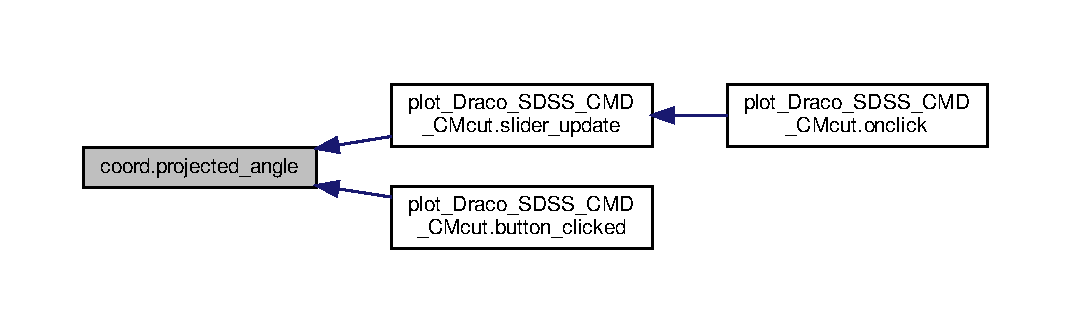
\includegraphics[width=350pt]{d2/df4/namespacecoord_a04a9b47f67924315930327ed806ee648_icgraph}
\end{center}
\end{figure}
\mbox{\Hypertarget{namespacecoord_a46aebc3089e078f4597812fecdd0975f}\label{namespacecoord_a46aebc3089e078f4597812fecdd0975f}} 
\index{coord@{coord}!projected\+\_\+distance@{projected\+\_\+distance}}
\index{projected\+\_\+distance@{projected\+\_\+distance}!coord@{coord}}
\subsubsection{\texorpdfstring{projected\+\_\+distance()}{projected\_distance()}}
{\footnotesize\ttfamily def coord.\+projected\+\_\+distance (\begin{DoxyParamCaption}\item[{}]{dist,  }\item[{}]{ra\+\_\+center,  }\item[{}]{de\+\_\+center,  }\item[{}]{ra,  }\item[{}]{de,  }\item[{}]{dtype = {\ttfamily \char`\"{}rad\char`\"{}} }\end{DoxyParamCaption})}

\begin{DoxyVerb}args:
    ra_center,de_center,ra,de: radian unit
note:
    calculate the projected distance from the center position:
    dist = dist*sin(theta),
    cos_theta = c(de_center)*c(de)*(c(ra-ra_center))+s(de_center)*s(de)
\end{DoxyVerb}
 

Definition at line 5 of file coord.\+py.


\begin{DoxyCode}
5 \textcolor{keyword}{def }\hyperlink{namespacecoord_a46aebc3089e078f4597812fecdd0975f}{projected\_distance}(dist,ra\_center,de\_center,ra,de,dtype="rad"):
6     \textcolor{stringliteral}{'''}
7 \textcolor{stringliteral}{    args:}
8 \textcolor{stringliteral}{        ra\_center,de\_center,ra,de: radian unit}
9 \textcolor{stringliteral}{    note:}
10 \textcolor{stringliteral}{        calculate the projected distance from the center position:}
11 \textcolor{stringliteral}{        dist = dist*sin(theta),}
12 \textcolor{stringliteral}{        cos\_theta = c(de\_center)*c(de)*(c(ra-ra\_center))+s(de\_center)*s(de)}
13 \textcolor{stringliteral}{    '''}
14     t = np.deg2rad \textcolor{keywordflow}{if} dtype == \textcolor{stringliteral}{"deg"} \textcolor{keywordflow}{else} \textcolor{keyword}{lambda} x:x
15     cos\_theta = c(t(de\_center))*c(t(de))*(c(t(ra-ra\_center)))+s(t(de\_center))*s(t(de))
16     \textcolor{keywordflow}{return} dist*np.sqrt(1-cos\_theta*cos\_theta)
17 
\end{DoxyCode}
Here is the caller graph for this function\+:\nopagebreak
\begin{figure}[H]
\begin{center}
\leavevmode
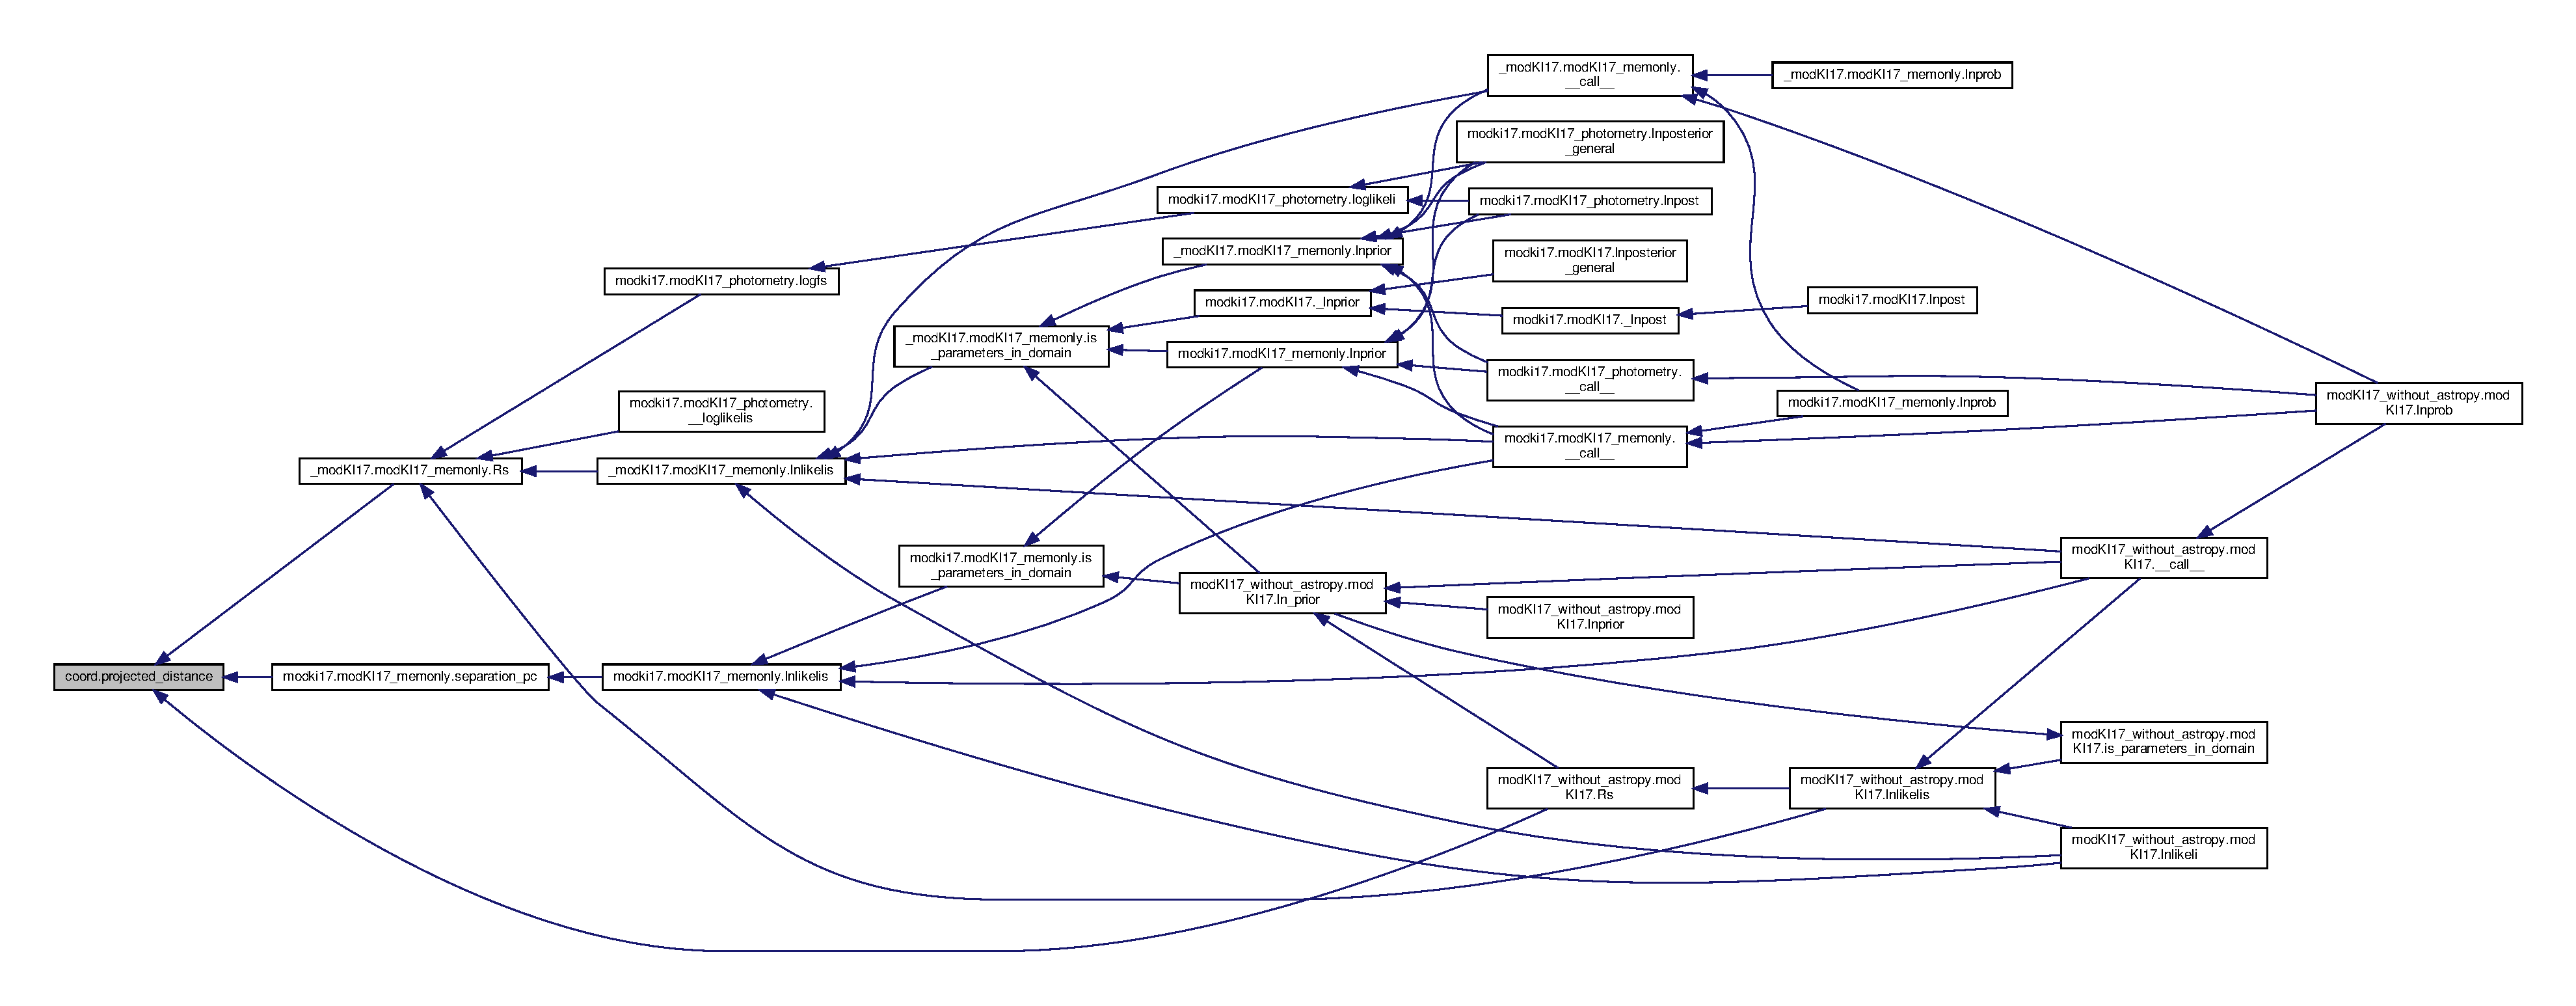
\includegraphics[width=350pt]{d2/df4/namespacecoord_a46aebc3089e078f4597812fecdd0975f_icgraph}
\end{center}
\end{figure}
\mbox{\Hypertarget{namespacecoord_a6cca1fe4ad65d56023a02550cbba8ce8}\label{namespacecoord_a6cca1fe4ad65d56023a02550cbba8ce8}} 
\index{coord@{coord}!projected\+\_\+distance\+\_\+simple@{projected\+\_\+distance\+\_\+simple}}
\index{projected\+\_\+distance\+\_\+simple@{projected\+\_\+distance\+\_\+simple}!coord@{coord}}
\subsubsection{\texorpdfstring{projected\+\_\+distance\+\_\+simple()}{projected\_distance\_simple()}}
{\footnotesize\ttfamily def coord.\+projected\+\_\+distance\+\_\+simple (\begin{DoxyParamCaption}\item[{}]{dist,  }\item[{}]{ra\+\_\+center,  }\item[{}]{de\+\_\+center,  }\item[{}]{ra,  }\item[{}]{de,  }\item[{}]{dtype = {\ttfamily \char`\"{}rad\char`\"{}} }\end{DoxyParamCaption})}

\begin{DoxyVerb}args:
    ra_center,de_center,ra,de: radian unit
note:
    calculate the projected distance from the center position:
    dist = dist*sin(theta),
    cos_theta = c(de_center)*c(de)*(c(ra-ra_center))+s(de_center)*s(de)
\end{DoxyVerb}
 

Definition at line 18 of file coord.\+py.


\begin{DoxyCode}
18 \textcolor{keyword}{def }\hyperlink{namespacecoord_a6cca1fe4ad65d56023a02550cbba8ce8}{projected\_distance\_simple}(dist,ra\_center,de\_center,ra,de,dtype="rad"):
19     \textcolor{stringliteral}{'''}
20 \textcolor{stringliteral}{    args:}
21 \textcolor{stringliteral}{        ra\_center,de\_center,ra,de: radian unit}
22 \textcolor{stringliteral}{    note:}
23 \textcolor{stringliteral}{        calculate the projected distance from the center position:}
24 \textcolor{stringliteral}{        dist = dist*sin(theta),}
25 \textcolor{stringliteral}{        cos\_theta = c(de\_center)*c(de)*(c(ra-ra\_center))+s(de\_center)*s(de)}
26 \textcolor{stringliteral}{    '''}
27     t = np.deg2rad \textcolor{keywordflow}{if} dtype == \textcolor{stringliteral}{"deg"} \textcolor{keywordflow}{else} \textcolor{keyword}{lambda} x:x
28     \textcolor{keywordflow}{return} dist*np.sqrt( (c(t(de\_center))*t(ra-ra\_center))**2 + (t(de-de\_center))**2 )
29 
\end{DoxyCode}


\subsection{Variable Documentation}
\mbox{\Hypertarget{namespacecoord_a87ee5c40fe361f2c1bfbea4ed5086028}\label{namespacecoord_a87ee5c40fe361f2c1bfbea4ed5086028}} 
\index{coord@{coord}!args@{args}}
\index{args@{args}!coord@{coord}}
\subsubsection{\texorpdfstring{args}{args}}
{\footnotesize\ttfamily dictionary coord.\+args = \{\textquotesingle{}ra\+\_\+center\textquotesingle{}\+:0,\textquotesingle{}de\+\_\+center\textquotesingle{}\+:np.\+pi/2-\/0.\+5\}}



Definition at line 64 of file coord.\+py.

\mbox{\Hypertarget{namespacecoord_a9aa399b274864850fc9b9569a1256848}\label{namespacecoord_a9aa399b274864850fc9b9569a1256848}} 
\index{coord@{coord}!ax@{ax}}
\index{ax@{ax}!coord@{coord}}
\subsubsection{\texorpdfstring{ax}{ax}}
{\footnotesize\ttfamily coord.\+ax = fig.\+add\+\_\+subplot(111,projection=\textquotesingle{}3d\textquotesingle{})}



Definition at line 71 of file coord.\+py.

\mbox{\Hypertarget{namespacecoord_a8dcc8c73e25f42279ad5b38825c9b285}\label{namespacecoord_a8dcc8c73e25f42279ad5b38825c9b285}} 
\index{coord@{coord}!de@{de}}
\index{de@{de}!coord@{coord}}
\subsubsection{\texorpdfstring{de}{de}}
{\footnotesize\ttfamily tuple coord.\+de = (np.\+arange(-\/np.\+pi,np.\+pi,0.\+01) + \hyperlink{namespacecoord_a87ee5c40fe361f2c1bfbea4ed5086028}{args}\mbox{[}\textquotesingle{}de\+\_\+center\textquotesingle{}\mbox{]})}



Definition at line 66 of file coord.\+py.

\mbox{\Hypertarget{namespacecoord_ae502575d54f9026dd1c6b0118fc65c63}\label{namespacecoord_ae502575d54f9026dd1c6b0118fc65c63}} 
\index{coord@{coord}!des@{des}}
\index{des@{des}!coord@{coord}}
\subsubsection{\texorpdfstring{des}{des}}
{\footnotesize\ttfamily coord.\+des}



Definition at line 67 of file coord.\+py.

\mbox{\Hypertarget{namespacecoord_a2314e07f943e13a24947dced6bee4b64}\label{namespacecoord_a2314e07f943e13a24947dced6bee4b64}} 
\index{coord@{coord}!dists@{dists}}
\index{dists@{dists}!coord@{coord}}
\subsubsection{\texorpdfstring{dists}{dists}}
{\footnotesize\ttfamily def coord.\+dists = \hyperlink{namespacecoord_a46aebc3089e078f4597812fecdd0975f}{projected\+\_\+distance}(1,\hyperlink{namespacecoord_a9e8cb473ba5d9c7398020447b51174e0}{ra}=\hyperlink{namespacecoord_a5462056be5c33668cdc23bd703b745c5}{ras},\hyperlink{namespacecoord_a8dcc8c73e25f42279ad5b38825c9b285}{de}=\hyperlink{namespacecoord_ae502575d54f9026dd1c6b0118fc65c63}{des},$\ast$$\ast$\hyperlink{namespacecoord_a87ee5c40fe361f2c1bfbea4ed5086028}{args})}



Definition at line 68 of file coord.\+py.

\mbox{\Hypertarget{namespacecoord_abd9b02ef552306f922eb3b6d0be56c34}\label{namespacecoord_abd9b02ef552306f922eb3b6d0be56c34}} 
\index{coord@{coord}!fig@{fig}}
\index{fig@{fig}!coord@{coord}}
\subsubsection{\texorpdfstring{fig}{fig}}
{\footnotesize\ttfamily coord.\+fig = plt.\+figure()}



Definition at line 70 of file coord.\+py.

\mbox{\Hypertarget{namespacecoord_a9e8cb473ba5d9c7398020447b51174e0}\label{namespacecoord_a9e8cb473ba5d9c7398020447b51174e0}} 
\index{coord@{coord}!ra@{ra}}
\index{ra@{ra}!coord@{coord}}
\subsubsection{\texorpdfstring{ra}{ra}}
{\footnotesize\ttfamily tuple coord.\+ra = (np.\+arange(-\/np.\+pi,np.\+pi,0.\+01) + \hyperlink{namespacecoord_a87ee5c40fe361f2c1bfbea4ed5086028}{args}\mbox{[}\textquotesingle{}ra\+\_\+center\textquotesingle{}\mbox{]})}



Definition at line 65 of file coord.\+py.

\mbox{\Hypertarget{namespacecoord_a5462056be5c33668cdc23bd703b745c5}\label{namespacecoord_a5462056be5c33668cdc23bd703b745c5}} 
\index{coord@{coord}!ras@{ras}}
\index{ras@{ras}!coord@{coord}}
\subsubsection{\texorpdfstring{ras}{ras}}
{\footnotesize\ttfamily coord.\+ras}



Definition at line 67 of file coord.\+py.


\hypertarget{namespacedequad}{}\section{dequad Namespace Reference}
\label{namespacedequad}\index{dequad@{dequad}}
\subsection*{Functions}
\begin{DoxyCompactItemize}
\item 
def \hyperlink{namespacedequad_a0774348e796cb0945f2e0b0a7fa1c1e9}{generate\+\_\+x\+\_\+w} (a, b, width, mN, pN, xp=np)
\item 
def \hyperlink{namespacedequad_a312cb2f278bec2760a7cb9a17bf3928f}{dequad} (func, a, b, width=5e-\/3, p\+N=1000, m\+N=1000, axis=\+None, kind=\char`\"{}linear\char`\"{}, dtype=float64, show\+\_\+fig=\+False, show\+\_\+integrand\+\_\+array=\+False, ignore\+\_\+nan=\+False, xp=np)
\item 
def \hyperlink{namespacedequad_a2654bb61f33ab8685320882396c81ae0}{dequad\+\_\+hinf} (func, a, width=5e-\/3, p\+N=1000, m\+N=1000, axis=\+None, kind=\char`\"{}linear\char`\"{}, dtype=float64, show\+\_\+fig=\+False, show\+\_\+integrand\+\_\+array=\+True)
\end{DoxyCompactItemize}
\subsection*{Variables}
\begin{DoxyCompactItemize}
\item 
bool \hyperlink{namespacedequad_a19fc97d6e01fffb74ca81c02a51d86c0}{D\+E\+B\+UG} = False
\item 
\hyperlink{namespacedequad_a7f2d7b33e38c6d5249b152740f656344}{B\+U\+F\+\_\+\+D\+E\+B\+UG} = None
\item 
\hyperlink{namespacedequad_aecd7501e851b01ca793cb5b896fa5141}{maxsize}
\end{DoxyCompactItemize}


\subsection{Function Documentation}
\mbox{\Hypertarget{namespacedequad_a312cb2f278bec2760a7cb9a17bf3928f}\label{namespacedequad_a312cb2f278bec2760a7cb9a17bf3928f}} 
\index{dequad@{dequad}!dequad@{dequad}}
\index{dequad@{dequad}!dequad@{dequad}}
\subsubsection{\texorpdfstring{dequad()}{dequad()}}
{\footnotesize\ttfamily def dequad.\+dequad (\begin{DoxyParamCaption}\item[{}]{func,  }\item[{}]{a,  }\item[{}]{b,  }\item[{}]{width = {\ttfamily 5e-\/3},  }\item[{}]{pN = {\ttfamily 1000},  }\item[{}]{mN = {\ttfamily 1000},  }\item[{}]{axis = {\ttfamily None},  }\item[{}]{kind = {\ttfamily \char`\"{}linear\char`\"{}},  }\item[{}]{dtype = {\ttfamily float64},  }\item[{}]{show\+\_\+fig = {\ttfamily False},  }\item[{}]{show\+\_\+integrand\+\_\+array = {\ttfamily False},  }\item[{}]{ignore\+\_\+nan = {\ttfamily False},  }\item[{}]{xp = {\ttfamily np} }\end{DoxyParamCaption})}

\begin{DoxyVerb}func: func(ndarray_in) = ndarray_out
axis: define the axis of ndarray_out to use integrate.

Note: If "func" is like func: array(n,) -> array(m,n),
          f(x) * w ~ (m,n) * (n,) ~ (m,n) * (1,n)
      then works well (axis should set as axis=1). 
\end{DoxyVerb}
 

Definition at line 36 of file dequad.\+py.


\begin{DoxyCode}
36 \textcolor{keyword}{def }\hyperlink{namespacedequad_a312cb2f278bec2760a7cb9a17bf3928f}{dequad}(
      func,a,b,width=5e-3,pN=1000,mN=1000,axis=None,kind="linear",dtype=float64,show\_fig=False,show\_integrand\_array=False,ignore\_nan=False,xp=np):
37     \textcolor{stringliteral}{'''}
38 \textcolor{stringliteral}{    func: func(ndarray\_in) = ndarray\_out}
39 \textcolor{stringliteral}{    axis: define the axis of ndarray\_out to use integrate.}
40 \textcolor{stringliteral}{    }
41 \textcolor{stringliteral}{    Note: If "func" is like func: array(n,) -> array(m,n),}
42 \textcolor{stringliteral}{              f(x) * w ~ (m,n) * (n,) ~ (m,n) * (1,n)}
43 \textcolor{stringliteral}{          then works well (axis should set as axis=1). }
44 \textcolor{stringliteral}{    '''}
45     \textcolor{keywordflow}{if} kind == \textcolor{stringliteral}{"linear"}:
46         \textcolor{comment}{#print(a,b,width,mN,pN)}
47         \textcolor{comment}{#print(generate\_x\_w(a,b,width,mN,pN,xp=np))}
48         xs,ws = \hyperlink{namespacedequad_a0774348e796cb0945f2e0b0a7fa1c1e9}{generate\_x\_w}(a,b,width,mN,pN,xp)
49         wsfs = ws*func(xs)
50         isnan = xp.isnan(wsfs)
51         isinf = xp.isinf(wsfs)
52         wsfs[isnan | isinf] = 0
53         
54         print(wsfs[wsfs!=0]) \textcolor{keywordflow}{if} DEBUG \textcolor{keywordflow}{else} \textcolor{keywordtype}{None}
55         
56         \textcolor{keywordflow}{if} np.any(isnan) \textcolor{keywordflow}{and} \textcolor{keywordflow}{not} ignore\_nan:
57             \textcolor{keywordflow}{raise} TypeError(\textcolor{stringliteral}{"dequad\_hinf: wsfs is nan! \{\}"}.format(wsfs))
58         \textcolor{keywordflow}{if} show\_fig:
59             \textcolor{keywordflow}{if} len(wsfs.shape)>1:
60                 np.set\_printoptions(threshold=20)
61                 display(wsfs) \textcolor{keywordflow}{if} show\_integrand\_array \textcolor{keywordflow}{else} \textcolor{keywordtype}{None}
62                 plt.plot(width*xp.arange(-mN,pN),wsfs.T)
63                 plt.legend(wsfs.sum(axis=axis))
64             \textcolor{keywordflow}{else}:
65                 plt.plot(ts,wsfs)
66         \textcolor{keywordflow}{return} (wsfs).sum(axis=axis)
67     \textcolor{keywordflow}{elif} kind == \textcolor{stringliteral}{"log"}:
68         \textcolor{stringliteral}{"""}
69 \textcolor{stringliteral}{        R = \(\backslash\)sum\_\{i=mN\}^\{pN\} w\_i * f(x\_i)}
70 \textcolor{stringliteral}{        """}
71         ts = width*arange(-mN,pN)
72         xs = exp(sinh(ts)*pi/2) + a
73         logwsp = log(width *pi/2) + ts + pi/2*sinh(ts)
74         logwsm = log(width *pi/2) - ts + pi/2*sinh(ts)
75         logfs = func(xs)
76         wsfs = (exp(logwsp*logfs)+exp(logwsm*logfs))/2
77         wsfs[isnan(wsfs) | isinf(wsfs)] = 0
78         \textcolor{keywordflow}{return} (wsfs).sum(axis=axis)
79 
\end{DoxyCode}
Here is the call graph for this function\+:\nopagebreak
\begin{figure}[H]
\begin{center}
\leavevmode
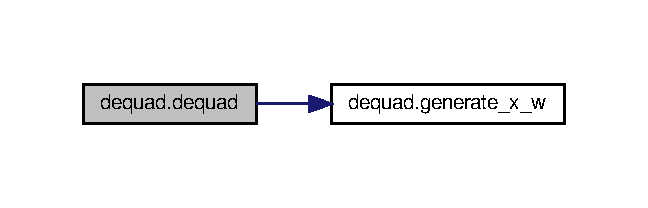
\includegraphics[width=311pt]{da/dfc/namespacedequad_a312cb2f278bec2760a7cb9a17bf3928f_cgraph}
\end{center}
\end{figure}
\mbox{\Hypertarget{namespacedequad_a2654bb61f33ab8685320882396c81ae0}\label{namespacedequad_a2654bb61f33ab8685320882396c81ae0}} 
\index{dequad@{dequad}!dequad\+\_\+hinf@{dequad\+\_\+hinf}}
\index{dequad\+\_\+hinf@{dequad\+\_\+hinf}!dequad@{dequad}}
\subsubsection{\texorpdfstring{dequad\+\_\+hinf()}{dequad\_hinf()}}
{\footnotesize\ttfamily def dequad.\+dequad\+\_\+hinf (\begin{DoxyParamCaption}\item[{}]{func,  }\item[{}]{a,  }\item[{}]{width = {\ttfamily 5e-\/3},  }\item[{}]{pN = {\ttfamily 1000},  }\item[{}]{mN = {\ttfamily 1000},  }\item[{}]{axis = {\ttfamily None},  }\item[{}]{kind = {\ttfamily \char`\"{}linear\char`\"{}},  }\item[{}]{dtype = {\ttfamily float64},  }\item[{}]{show\+\_\+fig = {\ttfamily False},  }\item[{}]{show\+\_\+integrand\+\_\+array = {\ttfamily True} }\end{DoxyParamCaption})}

\begin{DoxyVerb}func: func(ndarray_in) = ndarray_out
axis: define the axis of ndarray_out to use integrate.

Note: If "func" is like func: array(n,) -> array(m,n),
          f(x) * w ~ (m,n) * (n,) ~ (m,n) * (1,n)
      then works well (axis should set as axis=1). 
\end{DoxyVerb}
 

Definition at line 80 of file dequad.\+py.


\begin{DoxyCode}
80 \textcolor{keyword}{def }\hyperlink{namespacedequad_a2654bb61f33ab8685320882396c81ae0}{dequad\_hinf}(
      func,a,width=5e-3,pN=1000,mN=1000,axis=None,kind="linear",dtype=float64,show\_fig=False,show\_integrand\_array=True):
81     \textcolor{stringliteral}{'''}
82 \textcolor{stringliteral}{    func: func(ndarray\_in) = ndarray\_out}
83 \textcolor{stringliteral}{    axis: define the axis of ndarray\_out to use integrate.}
84 \textcolor{stringliteral}{    }
85 \textcolor{stringliteral}{    Note: If "func" is like func: array(n,) -> array(m,n),}
86 \textcolor{stringliteral}{              f(x) * w ~ (m,n) * (n,) ~ (m,n) * (1,n)}
87 \textcolor{stringliteral}{          then works well (axis should set as axis=1). }
88 \textcolor{stringliteral}{    '''}
89     \textcolor{keywordflow}{if} kind == \textcolor{stringliteral}{"linear"}:
90         xs,ws = \hyperlink{namespacedequad_a0774348e796cb0945f2e0b0a7fa1c1e9}{generate\_x\_w}(a,np.inf,width,mN,pN,xp=np)
91         wsfs = ws*func(xs)
92         isnan = np.isnan(wsfs)
93         isinf = np.isinf(wsfs)
94         wsfs[isnan | isinf] = 0
95         
96         print(wsfs[wsfs!=0]) \textcolor{keywordflow}{if} DEBUG \textcolor{keywordflow}{else} \textcolor{keywordtype}{None}
97         
98         \textcolor{keywordflow}{if} np.any(isnan):
99             \textcolor{keywordflow}{raise} TypeError(\textcolor{stringliteral}{"dequad\_hinf: wsfs is nan! \{\}"}.format(wsfs))
100         \textcolor{keywordflow}{if} show\_fig:
101             \textcolor{keywordflow}{if} len(wsfs.shape)>1:
102                 np.set\_printoptions(threshold=20)
103                 display(wsfs) \textcolor{keywordflow}{if} show\_integrand\_array \textcolor{keywordflow}{else} \textcolor{keywordtype}{None}
104                 plt.plot(width*np.arange(-mN,pN),*wsfs,label=(wsfs).sum(axis=axis))
105                 plt.legend()
106             \textcolor{keywordflow}{else}:
107                 plt.plot(ts,wsfs)
108         \textcolor{keywordflow}{return} (wsfs).sum(axis=axis)
109     \textcolor{keywordflow}{elif} kind == \textcolor{stringliteral}{"log"}:
110         \textcolor{stringliteral}{"""}
111 \textcolor{stringliteral}{        R = \(\backslash\)sum\_\{i=mN\}^\{pN\} w\_i * f(x\_i)}
112 \textcolor{stringliteral}{        """}
113         ts = width*arange(-mN,pN)
114         xs = exp(sinh(ts)*pi/2) + a
115         logwsp = log(width *pi/2) + ts + pi/2*sinh(ts)
116         logwsm = log(width *pi/2) - ts + pi/2*sinh(ts)
117         logfs = func(xs)
118         wsfs = (exp(logwsp*logfs)+exp(logwsm*logfs))/2
119         wsfs[isnan(wsfs) | isinf(wsfs)] = 0
120         \textcolor{keywordflow}{return} (wsfs).sum(axis=axis)
121 
122 \textcolor{stringliteral}{"""}
123 \textcolor{stringliteral}{def dequad\_hinf\_cupysum(func,a,width=5e-3,pN=1000,mN=1000,axis=None,kind="linear"
      ,dtype=float64,show\_fig=False,show\_integrand\_array=True,xp=np):}
124 \textcolor{stringliteral}{    '''}
125 \textcolor{stringliteral}{    func: func(ndarray\_in) = ndarray\_out}
126 \textcolor{stringliteral}{    axis: define the axis of ndarray\_out to use integrate.}
127 \textcolor{stringliteral}{    }
128 \textcolor{stringliteral}{    Note: If "func" is like func: array(n,) -> array(m,n),}
129 \textcolor{stringliteral}{              f(x) * w ~ (m,n) * (n,) ~ (m,n) * (1,n)}
130 \textcolor{stringliteral}{          then works well (axis should set as axis=1). }
131 \textcolor{stringliteral}{    '''}
132 \textcolor{stringliteral}{    }
133 \textcolor{stringliteral}{    stream = cupy.cuda.Stream.null}
134 \textcolor{stringliteral}{    start = stream.record()}
135 \textcolor{stringliteral}{    }
136 \textcolor{stringliteral}{    if kind == "linear":}
137 \textcolor{stringliteral}{        xs,ws = generate\_x\_w(a,width,mN,pN,xp)}
138 \textcolor{stringliteral}{        wsfs = cp.asarray(ws)*cp.asarray(func(xs))}
139 \textcolor{stringliteral}{        isnan = xp.isnan(wsfs)}
140 \textcolor{stringliteral}{        isinf = xp.isinf(wsfs)}
141 \textcolor{stringliteral}{        wsfs[isnan | isinf] = 0}
142 \textcolor{stringliteral}{        }
143 \textcolor{stringliteral}{        print(wsfs[wsfs!=0]) if DEBUG else None}
144 \textcolor{stringliteral}{        }
145 \textcolor{stringliteral}{        if xp.any(isnan):}
146 \textcolor{stringliteral}{            raise TypeError("dequad\_hinf: wsfs is nan! \{\}".format(wsfs))}
147 \textcolor{stringliteral}{        if show\_fig:}
148 \textcolor{stringliteral}{            if len(wsfs.shape)>1:}
149 \textcolor{stringliteral}{                np.set\_printoptions(threshold=20)}
150 \textcolor{stringliteral}{                display(wsfs) if show\_integrand\_array else None}
151 \textcolor{stringliteral}{                plt.plot(ts,*wsfs,label=(wsfs).sum(axis=axis))}
152 \textcolor{stringliteral}{                plt.legend()}
153 \textcolor{stringliteral}{            else:}
154 \textcolor{stringliteral}{                plt.plot(ts,wsfs)}
155 \textcolor{stringliteral}{}
156 \textcolor{stringliteral}{        end = stream.record()}
157 \textcolor{stringliteral}{        end.synchronize()}
158 \textcolor{stringliteral}{        elapsed = cupy.cuda.get\_elapsed\_time(start, end)}
159 \textcolor{stringliteral}{        #print(elapsed)}
160 \textcolor{stringliteral}{                }
161 \textcolor{stringliteral}{        return (wsfs).sum(axis=axis)}
162 \textcolor{stringliteral}{    elif kind == "log":}
163 \textcolor{stringliteral}{        '''}
164 \textcolor{stringliteral}{        R = \(\backslash\)sum\_\{i=mN\}^\{pN\} w\_i * f(x\_i)}
165 \textcolor{stringliteral}{        '''}
166 \textcolor{stringliteral}{        ts = width*arange(-mN,pN)}
167 \textcolor{stringliteral}{        xs = exp(sinh(ts)*pi/2) + a}
168 \textcolor{stringliteral}{        logwsp = log(width *pi/2) + ts + pi/2*sinh(ts)}
169 \textcolor{stringliteral}{        logwsm = log(width *pi/2) - ts + pi/2*sinh(ts)}
170 \textcolor{stringliteral}{        logfs = func(xs)}
171 \textcolor{stringliteral}{        wsfs = (exp(logwsp*logfs)+exp(logwsm*logfs))/2}
172 \textcolor{stringliteral}{        wsfs[isnan(wsfs) | isinf(wsfs)] = 0}
173 \textcolor{stringliteral}{        return (wsfs).sum(axis=axis)}
174 \textcolor{stringliteral}{"""}
175 \end{DoxyCode}
Here is the call graph for this function\+:\nopagebreak
\begin{figure}[H]
\begin{center}
\leavevmode
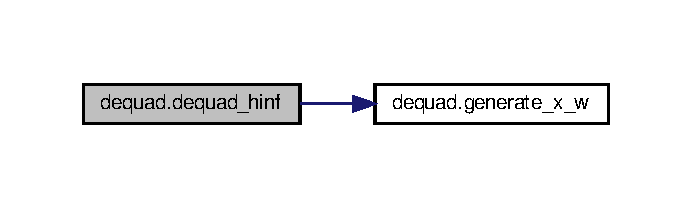
\includegraphics[width=332pt]{da/dfc/namespacedequad_a2654bb61f33ab8685320882396c81ae0_cgraph}
\end{center}
\end{figure}
Here is the caller graph for this function\+:\nopagebreak
\begin{figure}[H]
\begin{center}
\leavevmode
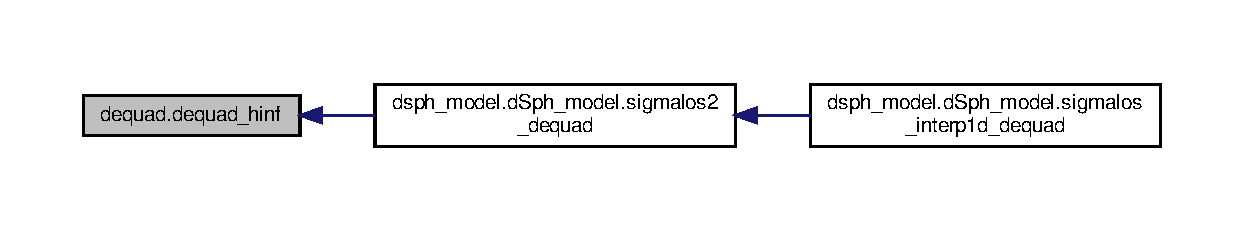
\includegraphics[width=350pt]{da/dfc/namespacedequad_a2654bb61f33ab8685320882396c81ae0_icgraph}
\end{center}
\end{figure}
\mbox{\Hypertarget{namespacedequad_a0774348e796cb0945f2e0b0a7fa1c1e9}\label{namespacedequad_a0774348e796cb0945f2e0b0a7fa1c1e9}} 
\index{dequad@{dequad}!generate\+\_\+x\+\_\+w@{generate\+\_\+x\+\_\+w}}
\index{generate\+\_\+x\+\_\+w@{generate\+\_\+x\+\_\+w}!dequad@{dequad}}
\subsubsection{\texorpdfstring{generate\+\_\+x\+\_\+w()}{generate\_x\_w()}}
{\footnotesize\ttfamily def dequad.\+generate\+\_\+x\+\_\+w (\begin{DoxyParamCaption}\item[{}]{a,  }\item[{}]{b,  }\item[{}]{width,  }\item[{}]{mN,  }\item[{}]{pN,  }\item[{}]{xp = {\ttfamily np} }\end{DoxyParamCaption})}

\begin{DoxyVerb}x = phi(t)
w = phi'(t)
\end{DoxyVerb}
 

Definition at line 11 of file dequad.\+py.


\begin{DoxyCode}
11 \textcolor{keyword}{def }\hyperlink{namespacedequad_a0774348e796cb0945f2e0b0a7fa1c1e9}{generate\_x\_w}(a,b,width,mN,pN,xp=np):
12     \textcolor{stringliteral}{'''}
13 \textcolor{stringliteral}{    x = phi(t)}
14 \textcolor{stringliteral}{    w = phi'(t)}
15 \textcolor{stringliteral}{    '''}
16     \textcolor{comment}{#print("generate\_x\_w in",a,b,width,mN,pN)}
17     pi2 = xp.pi/2
18     ts = width*xp.arange(-mN,pN)\textcolor{comment}{#.astype(dtype)}
19     \textcolor{keywordflow}{if} np.all(\textcolor{keywordflow}{not} np.isinf(a)) \textcolor{keywordflow}{and} np.all(np.isinf(b)):
20         ps = pi2*xp.sinh(ts)
21         xs = xp.exp(ps) + a
22         ws = width *pi2 *xp.cosh(ts)*xp.exp(ps)    
23         
24     \textcolor{keywordflow}{elif} np.all(np.isinf(a)) \textcolor{keywordflow}{and} np.all(np.isinf(b)):
25         ps = pi2*xp.sinh(ts)
26         xs = xp.sinh(ps)
27         ws = width *pi2 *xp.cosh(ts)*xp.cosh(ps)  
28         
29     \textcolor{keywordflow}{elif} np.all(\textcolor{keywordflow}{not} np.isinf(a)) \textcolor{keywordflow}{and} np.all(\textcolor{keywordflow}{not} np.isinf(b)):
30         ps = pi2*xp.sinh(ts)
31         xs = (b-a)/2*xp.tanh(ps) + (a+b)/2
32         ws = width * (b-a)/2 *pi2 *xp.cosh(ts)/(xp.cosh(ps)**2)
33         
34     \textcolor{keywordflow}{return} xs,ws
35 
\end{DoxyCode}
Here is the caller graph for this function\+:\nopagebreak
\begin{figure}[H]
\begin{center}
\leavevmode
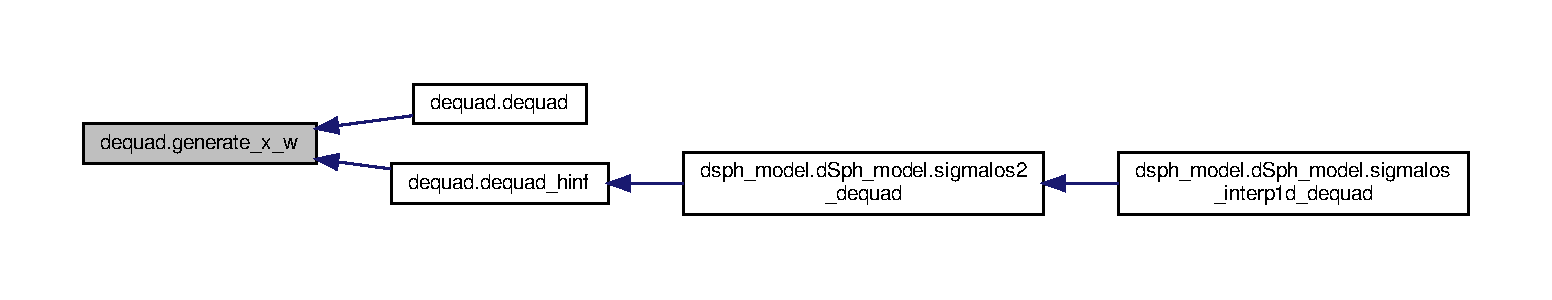
\includegraphics[width=350pt]{da/dfc/namespacedequad_a0774348e796cb0945f2e0b0a7fa1c1e9_icgraph}
\end{center}
\end{figure}


\subsection{Variable Documentation}
\mbox{\Hypertarget{namespacedequad_a7f2d7b33e38c6d5249b152740f656344}\label{namespacedequad_a7f2d7b33e38c6d5249b152740f656344}} 
\index{dequad@{dequad}!B\+U\+F\+\_\+\+D\+E\+B\+UG@{B\+U\+F\+\_\+\+D\+E\+B\+UG}}
\index{B\+U\+F\+\_\+\+D\+E\+B\+UG@{B\+U\+F\+\_\+\+D\+E\+B\+UG}!dequad@{dequad}}
\subsubsection{\texorpdfstring{B\+U\+F\+\_\+\+D\+E\+B\+UG}{BUF\_DEBUG}}
{\footnotesize\ttfamily dequad.\+B\+U\+F\+\_\+\+D\+E\+B\+UG = None}



Definition at line 8 of file dequad.\+py.

\mbox{\Hypertarget{namespacedequad_a19fc97d6e01fffb74ca81c02a51d86c0}\label{namespacedequad_a19fc97d6e01fffb74ca81c02a51d86c0}} 
\index{dequad@{dequad}!D\+E\+B\+UG@{D\+E\+B\+UG}}
\index{D\+E\+B\+UG@{D\+E\+B\+UG}!dequad@{dequad}}
\subsubsection{\texorpdfstring{D\+E\+B\+UG}{DEBUG}}
{\footnotesize\ttfamily bool dequad.\+D\+E\+B\+UG = False}



Definition at line 7 of file dequad.\+py.

\mbox{\Hypertarget{namespacedequad_aecd7501e851b01ca793cb5b896fa5141}\label{namespacedequad_aecd7501e851b01ca793cb5b896fa5141}} 
\index{dequad@{dequad}!maxsize@{maxsize}}
\index{maxsize@{maxsize}!dequad@{dequad}}
\subsubsection{\texorpdfstring{maxsize}{maxsize}}
{\footnotesize\ttfamily dequad.\+maxsize}



Definition at line 10 of file dequad.\+py.


\hypertarget{namespacedsph__model}{}\section{dsph\+\_\+model Namespace Reference}
\label{namespacedsph__model}\index{dsph\+\_\+model@{dsph\+\_\+model}}
\subsection*{Classes}
\begin{DoxyCompactItemize}
\item 
class \hyperlink{classdsph__model_1_1DM__model}{D\+M\+\_\+model}
\item 
class \hyperlink{classdsph__model_1_1dSph__model}{d\+Sph\+\_\+model}
\item 
class \hyperlink{classdsph__model_1_1exp2d__model}{exp2d\+\_\+model}
\item 
class \hyperlink{classdsph__model_1_1exp3d__model}{exp3d\+\_\+model}
\item 
class \hyperlink{classdsph__model_1_1KI17__model}{K\+I17\+\_\+model}
\item 
class \hyperlink{classdsph__model_1_1model}{model}
\item 
class \hyperlink{classdsph__model_1_1NFW__model}{N\+F\+W\+\_\+model}
\item 
class \hyperlink{classdsph__model_1_1plummer__model}{plummer\+\_\+model}
\item 
class \hyperlink{classdsph__model_1_1sersic__model}{sersic\+\_\+model}
\item 
class \hyperlink{classdsph__model_1_1stellar__model}{stellar\+\_\+model}
\item 
class \hyperlink{classdsph__model_1_1uniform2d__model}{uniform2d\+\_\+model}
\end{DoxyCompactItemize}
\subsection*{Variables}
\begin{DoxyCompactItemize}
\item 
float \hyperlink{namespacedsph__model_a783ea3c074de2e7c951b342b5749a522}{G\+Msun\+\_\+m3s2} = 1.\+32712440018e20
\item 
int \hyperlink{namespacedsph__model_a03ec56ecf56f64e59a6be020a76a36f1}{R\+\_\+trunc\+\_\+pc} = 1866.
\item 
\hyperlink{namespacedsph__model_a83bb8253e5a6c16c6d8f2b3ae8643576}{dm\+\_\+model} = \hyperlink{classdsph__model_1_1NFW__model}{N\+F\+W\+\_\+model}(a=2.\+78,b=7.\+78,g=0.\+675,rhos\+\_\+\+Msunpc3=np.\+power(10,-\/2.\+05),rs\+\_\+pc=np.\+power(10,3.\+96),\hyperlink{namespacedsph__model_a03ec56ecf56f64e59a6be020a76a36f1}{R\+\_\+trunc\+\_\+pc}=2000)
\item 
\hyperlink{namespacedsph__model_af9dc9391755a4aee2481a666d18e218a}{mystellar\+\_\+model} = \hyperlink{classdsph__model_1_1plummer__model}{plummer\+\_\+model}(re\+\_\+pc=221)
\item 
\hyperlink{namespacedsph__model_ab28142aa13968c1b7647e1fccabec0c6}{draco\+\_\+model} = \hyperlink{classdsph__model_1_1dSph__model}{d\+Sph\+\_\+model}(submodels\+\_\+dict=\{\char`\"{}D\+M\+\_\+model\char`\"{}\+:dm\+\_\+model,\char`\"{}stellar\+\_\+model\char`\"{}\+:mystellar\+\_\+model\},anib=1-\/np.\+power(10,0.\+13),dist\+\_\+center\+\_\+pc=76e3,ra\+\_\+center\+\_\+deg=0,de\+\_\+center\+\_\+deg=0)
\item 
\hyperlink{namespacedsph__model_af25a421d0de32d247b1aa0e8cf4894e3}{Rs} = np.\+logspace(-\/1,9,100)
\item 
\hyperlink{namespacedsph__model_a47e0439ddc091a015abf3612c9ee26c3}{ss} = draco\+\_\+model.\+sigmalos2(\hyperlink{namespacedsph__model_af25a421d0de32d247b1aa0e8cf4894e3}{Rs})
\item 
list \hyperlink{namespacedsph__model_abcaee14ea865b10f10051c500197bd4d}{ss2} = \mbox{[}draco\+\_\+model.\+sigmar2(R) for R in \hyperlink{namespacedsph__model_af25a421d0de32d247b1aa0e8cf4894e3}{Rs}\mbox{]}
\item 
list \hyperlink{namespacedsph__model_a570b90342742f8795c9affea98066d87}{ss3} = \mbox{[}draco\+\_\+model.\+naive\+\_\+sigmalos2(R) for R in \hyperlink{namespacedsph__model_af25a421d0de32d247b1aa0e8cf4894e3}{Rs}\mbox{]}
\end{DoxyCompactItemize}


\subsection{Variable Documentation}
\mbox{\Hypertarget{namespacedsph__model_a83bb8253e5a6c16c6d8f2b3ae8643576}\label{namespacedsph__model_a83bb8253e5a6c16c6d8f2b3ae8643576}} 
\index{dsph\+\_\+model@{dsph\+\_\+model}!dm\+\_\+model@{dm\+\_\+model}}
\index{dm\+\_\+model@{dm\+\_\+model}!dsph\+\_\+model@{dsph\+\_\+model}}
\subsubsection{\texorpdfstring{dm\+\_\+model}{dm\_model}}
{\footnotesize\ttfamily dsph\+\_\+model.\+dm\+\_\+model = \hyperlink{classdsph__model_1_1NFW__model}{N\+F\+W\+\_\+model}(a=2.\+78,b=7.\+78,g=0.\+675,rhos\+\_\+\+Msunpc3=np.\+power(10,-\/2.\+05),rs\+\_\+pc=np.\+power(10,3.\+96),\hyperlink{namespacedsph__model_a03ec56ecf56f64e59a6be020a76a36f1}{R\+\_\+trunc\+\_\+pc}=2000)}



Definition at line 524 of file dsph\+\_\+model.\+py.

\mbox{\Hypertarget{namespacedsph__model_ab28142aa13968c1b7647e1fccabec0c6}\label{namespacedsph__model_ab28142aa13968c1b7647e1fccabec0c6}} 
\index{dsph\+\_\+model@{dsph\+\_\+model}!draco\+\_\+model@{draco\+\_\+model}}
\index{draco\+\_\+model@{draco\+\_\+model}!dsph\+\_\+model@{dsph\+\_\+model}}
\subsubsection{\texorpdfstring{draco\+\_\+model}{draco\_model}}
{\footnotesize\ttfamily dsph\+\_\+model.\+draco\+\_\+model = \hyperlink{classdsph__model_1_1dSph__model}{d\+Sph\+\_\+model}(submodels\+\_\+dict=\{\char`\"{}D\+M\+\_\+model\char`\"{}\+:dm\+\_\+model,\char`\"{}stellar\+\_\+model\char`\"{}\+:mystellar\+\_\+model\},anib=1-\/np.\+power(10,0.\+13),dist\+\_\+center\+\_\+pc=76e3,ra\+\_\+center\+\_\+deg=0,de\+\_\+center\+\_\+deg=0)}



Definition at line 526 of file dsph\+\_\+model.\+py.

\mbox{\Hypertarget{namespacedsph__model_a783ea3c074de2e7c951b342b5749a522}\label{namespacedsph__model_a783ea3c074de2e7c951b342b5749a522}} 
\index{dsph\+\_\+model@{dsph\+\_\+model}!G\+Msun\+\_\+m3s2@{G\+Msun\+\_\+m3s2}}
\index{G\+Msun\+\_\+m3s2@{G\+Msun\+\_\+m3s2}!dsph\+\_\+model@{dsph\+\_\+model}}
\subsubsection{\texorpdfstring{G\+Msun\+\_\+m3s2}{GMsun\_m3s2}}
{\footnotesize\ttfamily float dsph\+\_\+model.\+G\+Msun\+\_\+m3s2 = 1.\+32712440018e20}



Definition at line 17 of file dsph\+\_\+model.\+py.

\mbox{\Hypertarget{namespacedsph__model_af9dc9391755a4aee2481a666d18e218a}\label{namespacedsph__model_af9dc9391755a4aee2481a666d18e218a}} 
\index{dsph\+\_\+model@{dsph\+\_\+model}!mystellar\+\_\+model@{mystellar\+\_\+model}}
\index{mystellar\+\_\+model@{mystellar\+\_\+model}!dsph\+\_\+model@{dsph\+\_\+model}}
\subsubsection{\texorpdfstring{mystellar\+\_\+model}{mystellar\_model}}
{\footnotesize\ttfamily dsph\+\_\+model.\+mystellar\+\_\+model = \hyperlink{classdsph__model_1_1plummer__model}{plummer\+\_\+model}(re\+\_\+pc=221)}



Definition at line 525 of file dsph\+\_\+model.\+py.

\mbox{\Hypertarget{namespacedsph__model_a03ec56ecf56f64e59a6be020a76a36f1}\label{namespacedsph__model_a03ec56ecf56f64e59a6be020a76a36f1}} 
\index{dsph\+\_\+model@{dsph\+\_\+model}!R\+\_\+trunc\+\_\+pc@{R\+\_\+trunc\+\_\+pc}}
\index{R\+\_\+trunc\+\_\+pc@{R\+\_\+trunc\+\_\+pc}!dsph\+\_\+model@{dsph\+\_\+model}}
\subsubsection{\texorpdfstring{R\+\_\+trunc\+\_\+pc}{R\_trunc\_pc}}
{\footnotesize\ttfamily int dsph\+\_\+model.\+R\+\_\+trunc\+\_\+pc = 1866.}



Definition at line 18 of file dsph\+\_\+model.\+py.

\mbox{\Hypertarget{namespacedsph__model_af25a421d0de32d247b1aa0e8cf4894e3}\label{namespacedsph__model_af25a421d0de32d247b1aa0e8cf4894e3}} 
\index{dsph\+\_\+model@{dsph\+\_\+model}!Rs@{Rs}}
\index{Rs@{Rs}!dsph\+\_\+model@{dsph\+\_\+model}}
\subsubsection{\texorpdfstring{Rs}{Rs}}
{\footnotesize\ttfamily dsph\+\_\+model.\+Rs = np.\+logspace(-\/1,9,100)}



Definition at line 528 of file dsph\+\_\+model.\+py.

\mbox{\Hypertarget{namespacedsph__model_a47e0439ddc091a015abf3612c9ee26c3}\label{namespacedsph__model_a47e0439ddc091a015abf3612c9ee26c3}} 
\index{dsph\+\_\+model@{dsph\+\_\+model}!ss@{ss}}
\index{ss@{ss}!dsph\+\_\+model@{dsph\+\_\+model}}
\subsubsection{\texorpdfstring{ss}{ss}}
{\footnotesize\ttfamily dsph\+\_\+model.\+ss = draco\+\_\+model.\+sigmalos2(\hyperlink{namespacedsph__model_af25a421d0de32d247b1aa0e8cf4894e3}{Rs})}



Definition at line 529 of file dsph\+\_\+model.\+py.

\mbox{\Hypertarget{namespacedsph__model_abcaee14ea865b10f10051c500197bd4d}\label{namespacedsph__model_abcaee14ea865b10f10051c500197bd4d}} 
\index{dsph\+\_\+model@{dsph\+\_\+model}!ss2@{ss2}}
\index{ss2@{ss2}!dsph\+\_\+model@{dsph\+\_\+model}}
\subsubsection{\texorpdfstring{ss2}{ss2}}
{\footnotesize\ttfamily list dsph\+\_\+model.\+ss2 = \mbox{[}draco\+\_\+model.\+sigmar2(R) for R in \hyperlink{namespacedsph__model_af25a421d0de32d247b1aa0e8cf4894e3}{Rs}\mbox{]}}



Definition at line 530 of file dsph\+\_\+model.\+py.

\mbox{\Hypertarget{namespacedsph__model_a570b90342742f8795c9affea98066d87}\label{namespacedsph__model_a570b90342742f8795c9affea98066d87}} 
\index{dsph\+\_\+model@{dsph\+\_\+model}!ss3@{ss3}}
\index{ss3@{ss3}!dsph\+\_\+model@{dsph\+\_\+model}}
\subsubsection{\texorpdfstring{ss3}{ss3}}
{\footnotesize\ttfamily list dsph\+\_\+model.\+ss3 = \mbox{[}draco\+\_\+model.\+naive\+\_\+sigmalos2(R) for R in \hyperlink{namespacedsph__model_af25a421d0de32d247b1aa0e8cf4894e3}{Rs}\mbox{]}}



Definition at line 531 of file dsph\+\_\+model.\+py.


\hypertarget{namespacedsphdata}{}\section{dsphdata Namespace Reference}
\label{namespacedsphdata}\index{dsphdata@{dsphdata}}
\subsection*{Classes}
\begin{DoxyCompactItemize}
\item 
class \hyperlink{classdsphdata_1_1dSphData}{d\+Sph\+Data}
\item 
class \hyperlink{classdsphdata_1_1dSphProp}{d\+Sph\+Prop}
\end{DoxyCompactItemize}

\hypertarget{namespaceinpoly}{}\section{inpoly Namespace Reference}
\label{namespaceinpoly}\index{inpoly@{inpoly}}
\subsection*{Functions}
\begin{DoxyCompactItemize}
\item 
def \hyperlink{namespaceinpoly_ac011fa801ecb6cc9429eaf02b25dd1e5}{inpolygon} (sx, sy, x, y)
\item 
def \hyperlink{namespaceinpoly_ad77175adc1811d9ba49b3a6f5753e336}{inpoly} (sx, sy, x, y, verbose=False)
\item 
def \hyperlink{namespaceinpoly_a6071c414de973f7a1162ae911036c02d}{cut} (data\+\_\+fname, poly\+\_\+fname, x\+\_\+data, y\+\_\+data, x\+\_\+poly, y\+\_\+poly, kwargs\+\_\+data=None, kwargs\+\_\+poly=None)
\end{DoxyCompactItemize}


\subsection{Function Documentation}
\mbox{\Hypertarget{namespaceinpoly_a6071c414de973f7a1162ae911036c02d}\label{namespaceinpoly_a6071c414de973f7a1162ae911036c02d}} 
\index{inpoly@{inpoly}!cut@{cut}}
\index{cut@{cut}!inpoly@{inpoly}}
\subsubsection{\texorpdfstring{cut()}{cut()}}
{\footnotesize\ttfamily def inpoly.\+cut (\begin{DoxyParamCaption}\item[{}]{data\+\_\+fname,  }\item[{}]{poly\+\_\+fname,  }\item[{}]{x\+\_\+data,  }\item[{}]{y\+\_\+data,  }\item[{}]{x\+\_\+poly,  }\item[{}]{y\+\_\+poly,  }\item[{}]{kwargs\+\_\+data = {\ttfamily None},  }\item[{}]{kwargs\+\_\+poly = {\ttfamily None} }\end{DoxyParamCaption})}



Definition at line 45 of file inpoly.\+py.


\begin{DoxyCode}
45 \textcolor{keyword}{def }\hyperlink{namespaceinpoly_a6071c414de973f7a1162ae911036c02d}{cut}(data\_fname,poly\_fname,x\_data,y\_data,x\_poly,y\_poly,kwargs\_data=None,kwargs\_poly=None):
46     data = read\_csv(data\_fname,**kwargs\_data)
47     poly = read\_csv(poly\_fname,**kwargs\_poly)
48     \textcolor{keywordflow}{return} \hyperlink{namespaceinpoly}{inpoly}(data[x\_data],data[y\_data],poly[x\_poly],data[x\_poly])
\end{DoxyCode}
\mbox{\Hypertarget{namespaceinpoly_ad77175adc1811d9ba49b3a6f5753e336}\label{namespaceinpoly_ad77175adc1811d9ba49b3a6f5753e336}} 
\index{inpoly@{inpoly}!inpoly@{inpoly}}
\index{inpoly@{inpoly}!inpoly@{inpoly}}
\subsubsection{\texorpdfstring{inpoly()}{inpoly()}}
{\footnotesize\ttfamily def inpoly.\+inpoly (\begin{DoxyParamCaption}\item[{}]{sx,  }\item[{}]{sy,  }\item[{}]{x,  }\item[{}]{y,  }\item[{}]{verbose = {\ttfamily False} }\end{DoxyParamCaption})}

\begin{DoxyVerb}x[:], y[:]: polygon
sx, sy: point
\end{DoxyVerb}
 

Definition at line 23 of file inpoly.\+py.


\begin{DoxyCode}
23 \textcolor{keyword}{def }\hyperlink{namespaceinpoly_ad77175adc1811d9ba49b3a6f5753e336}{inpoly}(sx,sy,x,y,verbose=False):
24     \textcolor{stringliteral}{''' }
25 \textcolor{stringliteral}{    x[:], y[:]: polygon}
26 \textcolor{stringliteral}{    sx, sy: point}
27 \textcolor{stringliteral}{    '''}    
28     x1 = x[:,np.newaxis]
29     y1 = y[:,np.newaxis]
30     x2 = np.roll(x1,-1)
31     y2 = np.roll(y1,-1)
32     \textcolor{keywordflow}{if} verbose:
33         print(np.array([x1[:,0],y1[:,0]]))
34         print(np.array([x2[:,0],y2[:,0]]))
35     ispointbetweenithsep = (x1-sx)*(x2-sx)<0
36     ispointaboveithsep = (x2-x1)*((x2-x1)*(sy-y1)-(y2-y1)*(sx-x1))>0
37     numofsepbelowpoint = (ispointbetweenithsep*ispointaboveithsep).sum(axis=0)
38     isoddnumbersepabovepoint = (numofsepbelowpoint%2 == 1)
39     \textcolor{comment}{#print(ispointbetweenithsep)}
40     \textcolor{comment}{#print(ispointaboveithsep)}
41     \textcolor{comment}{#print(numofsepbelowpoint)}
42     \textcolor{comment}{#print(isoddnumbersepabovepoint)}
43     \textcolor{keywordflow}{return} isoddnumbersepabovepoint
44 
\end{DoxyCode}
\mbox{\Hypertarget{namespaceinpoly_ac011fa801ecb6cc9429eaf02b25dd1e5}\label{namespaceinpoly_ac011fa801ecb6cc9429eaf02b25dd1e5}} 
\index{inpoly@{inpoly}!inpolygon@{inpolygon}}
\index{inpolygon@{inpolygon}!inpoly@{inpoly}}
\subsubsection{\texorpdfstring{inpolygon()}{inpolygon()}}
{\footnotesize\ttfamily def inpoly.\+inpolygon (\begin{DoxyParamCaption}\item[{}]{sx,  }\item[{}]{sy,  }\item[{}]{x,  }\item[{}]{y }\end{DoxyParamCaption})}

\begin{DoxyVerb}x[:], y[:]: polygon
sx, sy: point
\end{DoxyVerb}
 

Definition at line 4 of file inpoly.\+py.


\begin{DoxyCode}
4 \textcolor{keyword}{def }\hyperlink{namespaceinpoly_ac011fa801ecb6cc9429eaf02b25dd1e5}{inpolygon}(sx, sy, x, y):
5     \textcolor{stringliteral}{''' }
6 \textcolor{stringliteral}{    x[:], y[:]: polygon}
7 \textcolor{stringliteral}{    sx, sy: point}
8 \textcolor{stringliteral}{    '''}     
9     np = len(x)
10     inside = \textcolor{keyword}{False}
11     \textcolor{keywordflow}{for} i1 \textcolor{keywordflow}{in} range(np): 
12         i2 = (i1+1)%np
13         \textcolor{keywordflow}{if} min(x[i1], x[i2]) < sx < max(x[i1], x[i2]):
14             \textcolor{comment}{#a = (y[i2]-y[i1])/(x[i2]-x[i1])}
15             \textcolor{comment}{#b = y[i1] - a*x[i1]}
16             \textcolor{comment}{#dy = a*sx+b - sy}
17             \textcolor{comment}{#if dy >= 0:}
18             \textcolor{keywordflow}{if} (y[i1] + (y[i2]-y[i1])/(x[i2]-x[i1])*(sx-x[i1]) - sy) > 0:
19                 inside = \textcolor{keywordflow}{not} inside
20 
21     \textcolor{keywordflow}{return} inside
22 
\end{DoxyCode}

\hypertarget{namespacejfactor}{}\section{jfactor Namespace Reference}
\label{namespacejfactor}\index{jfactor@{jfactor}}
\subsection*{Functions}
\begin{DoxyCompactItemize}
\item 
def \hyperlink{namespacejfactor_ae5aad7f2ac90b82740c027677d7f4ac7}{Rroi\+\_\+pc} (dist)
\item 
def \hyperlink{namespacejfactor_aa60ca47daf4f993e2cc8bd268f7b206d}{rho\+\_\+\+Msunpc3} (r\+\_\+pc, \hyperlink{namespacejfactor_aa9f6835eba853a5bb2b380ad7fb87010}{rhos\+\_\+\+Msunpc3}, \hyperlink{namespacejfactor_ae602db7ab45f472ad4007d04def859f7}{rs\+\_\+pc}, \hyperlink{namespacejfactor_ab5ce4a1ef962b5f938f157d0abc69a20}{a}, \hyperlink{namespacejfactor_a52f3e9e591dbe4f5d14f760a578cb15b}{b}, \hyperlink{namespacejfactor_a1e07b351e264fceb00b01b4a591e45e5}{g})
\item 
def \hyperlink{namespacejfactor_afb33d5b3499565b8b7c23e15f3615ec0}{integrand\+\_\+err\+\_\+\+Jfactor} (r\+\_\+pc, \hyperlink{namespacejfactor_aa9f6835eba853a5bb2b380ad7fb87010}{rhos\+\_\+\+Msunpc3}, \hyperlink{namespacejfactor_ae602db7ab45f472ad4007d04def859f7}{rs\+\_\+pc}, \hyperlink{namespacejfactor_ab5ce4a1ef962b5f938f157d0abc69a20}{a}, \hyperlink{namespacejfactor_a52f3e9e591dbe4f5d14f760a578cb15b}{b}, \hyperlink{namespacejfactor_a1e07b351e264fceb00b01b4a591e45e5}{g}, dist)
\item 
def \hyperlink{namespacejfactor_ad8b8ed7dec1d2c3b4432d37e53117f03}{Jfactor\+\_\+err} (\hyperlink{namespacejfactor_aa9f6835eba853a5bb2b380ad7fb87010}{rhos\+\_\+\+Msunpc3}, \hyperlink{namespacejfactor_ae602db7ab45f472ad4007d04def859f7}{rs\+\_\+pc}, \hyperlink{namespacejfactor_ab5ce4a1ef962b5f938f157d0abc69a20}{a}, \hyperlink{namespacejfactor_a52f3e9e591dbe4f5d14f760a578cb15b}{b}, \hyperlink{namespacejfactor_a1e07b351e264fceb00b01b4a591e45e5}{g}, dist, Rtrunc\+\_\+pc=2000)
\item 
def \hyperlink{namespacejfactor_a4d9eb98f6dca866cd6248ef6b1c308a5}{Jfactor\+\_\+err\+\_\+dequad} (\hyperlink{namespacejfactor_aa9f6835eba853a5bb2b380ad7fb87010}{rhos\+\_\+\+Msunpc3}, \hyperlink{namespacejfactor_ae602db7ab45f472ad4007d04def859f7}{rs\+\_\+pc}, \hyperlink{namespacejfactor_ab5ce4a1ef962b5f938f157d0abc69a20}{a}, \hyperlink{namespacejfactor_a52f3e9e591dbe4f5d14f760a578cb15b}{b}, \hyperlink{namespacejfactor_a1e07b351e264fceb00b01b4a591e45e5}{g}, dist, Rtrunc\+\_\+pc=2000, width=5e-\/3, p\+N=1000, m\+N=1000, show\+\_\+fig=\+True)
\item 
def \hyperlink{namespacejfactor_aeb50ca469052983461a3e8382cfb4f95}{Jfactor\+\_\+v01} (\hyperlink{namespacejfactor_aa9f6835eba853a5bb2b380ad7fb87010}{rhos\+\_\+\+Msunpc3}, \hyperlink{namespacejfactor_ae602db7ab45f472ad4007d04def859f7}{rs\+\_\+pc}, \hyperlink{namespacejfactor_ab5ce4a1ef962b5f938f157d0abc69a20}{a}, \hyperlink{namespacejfactor_a52f3e9e591dbe4f5d14f760a578cb15b}{b}, \hyperlink{namespacejfactor_a1e07b351e264fceb00b01b4a591e45e5}{g}, dist)
\item 
def \hyperlink{namespacejfactor_afd0f5558d89189557900a6a1503261b3}{Jfactor\+\_\+v01\+\_\+truncated} (\hyperlink{namespacejfactor_aa9f6835eba853a5bb2b380ad7fb87010}{rhos\+\_\+\+Msunpc3}, \hyperlink{namespacejfactor_ae602db7ab45f472ad4007d04def859f7}{rs\+\_\+pc}, \hyperlink{namespacejfactor_ab5ce4a1ef962b5f938f157d0abc69a20}{a}, \hyperlink{namespacejfactor_a52f3e9e591dbe4f5d14f760a578cb15b}{b}, \hyperlink{namespacejfactor_a1e07b351e264fceb00b01b4a591e45e5}{g}, dist, Rtrunc\+\_\+pc=2000)
\item 
def \hyperlink{namespacejfactor_aaa43ebb0d9314fc697123b204465286e}{Jfactor\+\_\+v02} (\hyperlink{namespacejfactor_aa9f6835eba853a5bb2b380ad7fb87010}{rhos\+\_\+\+Msunpc3}, \hyperlink{namespacejfactor_ae602db7ab45f472ad4007d04def859f7}{rs\+\_\+pc}, \hyperlink{namespacejfactor_ab5ce4a1ef962b5f938f157d0abc69a20}{a}, \hyperlink{namespacejfactor_a52f3e9e591dbe4f5d14f760a578cb15b}{b}, \hyperlink{namespacejfactor_a1e07b351e264fceb00b01b4a591e45e5}{g}, dist, Rtrunc\+\_\+pc=2000)
\item 
def \hyperlink{namespacejfactor_a3261c30e40781120e1cacf7721893cb7}{Jfactor} (\hyperlink{namespacejfactor_aa9f6835eba853a5bb2b380ad7fb87010}{rhos\+\_\+\+Msunpc3}, \hyperlink{namespacejfactor_ae602db7ab45f472ad4007d04def859f7}{rs\+\_\+pc}, \hyperlink{namespacejfactor_ab5ce4a1ef962b5f938f157d0abc69a20}{a}, \hyperlink{namespacejfactor_a52f3e9e591dbe4f5d14f760a578cb15b}{b}, \hyperlink{namespacejfactor_a1e07b351e264fceb00b01b4a591e45e5}{g}, dist, Rtrunc\+\_\+pc=2000, return\+\_\+relerr=False, width=5e-\/3, p\+N=1000, m\+N=1000, show\+\_\+fig=\+False)
\end{DoxyCompactItemize}
\subsection*{Variables}
\begin{DoxyCompactItemize}
\item 
int \hyperlink{namespacejfactor_a2881505111ca34d6a84a5b09a5c19a86}{kg\+\_\+eV} = 1./physical\+\_\+constants\mbox{[}\char`\"{}electron volt-\/kilogram relationship\char`\"{}\mbox{]}\mbox{[}0\mbox{]}
\item 
int \hyperlink{namespacejfactor_a3d86861d725265dc096b798369902d43}{im\+\_\+eV} = 1./physical\+\_\+constants\mbox{[}\char`\"{}electron volt-\/inverse meter relationship\char`\"{}\mbox{]}\mbox{[}0\mbox{]}
\item 
float \hyperlink{namespacejfactor_a30f254edbd584a30535a1b98c2916563}{solar\+\_\+mass\+\_\+kg} = 1.\+9884e30
\item 
tuple \hyperlink{namespacejfactor_a69776fb72a257bd354abf1104511a3c7}{C0} = (\hyperlink{namespacejfactor_a30f254edbd584a30535a1b98c2916563}{solar\+\_\+mass\+\_\+kg}$\ast$\hyperlink{namespacejfactor_a2881505111ca34d6a84a5b09a5c19a86}{kg\+\_\+eV})$\ast$$\ast$2$\ast$((1./parsec)$\ast$\hyperlink{namespacejfactor_a3d86861d725265dc096b798369902d43}{im\+\_\+eV})$\ast$$\ast$5
\item 
tuple \hyperlink{namespacejfactor_a2c0c80a124f7a32f943f0b9b38f184d4}{C1} = (1e9)$\ast$$\ast$2 $\ast$ (1e2$\ast$im\+\_\+e\+V)$\ast$$\ast$5
\item 
tuple \hyperlink{namespacejfactor_aaa482b21aae986b864a5adb04d928dab}{C\+\_\+J} = \hyperlink{namespacejfactor_a69776fb72a257bd354abf1104511a3c7}{C0}/\hyperlink{namespacejfactor_a2c0c80a124f7a32f943f0b9b38f184d4}{C1}
\item 
\hyperlink{namespacejfactor_abfd9403bf30810505dc44d7af9746a12}{Jfactor\+\_\+v02} = np.\+vectorize(Jfactor\+\_\+v02)
\item 
\hyperlink{namespacejfactor_a2f38906b89281fb8e6cdc4cbc9c8735e}{argvs} = sys.\+argv
\item 
\hyperlink{namespacejfactor_a7ec02594672c6b2a0a519df5a7648ce2}{argc} = len(\hyperlink{namespacejfactor_a2f38906b89281fb8e6cdc4cbc9c8735e}{argvs})
\item 
list \hyperlink{namespacejfactor_a32ed195f2e906262c560b25bbc440b00}{log\+M\+Cparams\+\_\+filenames\+\_\+list} = \mbox{[}glob.\+glob(argv) for argv in \hyperlink{namespacejfactor_a2f38906b89281fb8e6cdc4cbc9c8735e}{argvs}\mbox{[}1\+:\mbox{]}\mbox{]}
\item 
\hyperlink{namespacejfactor_a025ed272933b6b6f31f688649810e704}{log\+M\+Cparams\+\_\+list} = np.\+array(\mbox{[}np.\+loadtxt(log\+M\+Cparams\+\_\+filename,delimiter=\textquotesingle{},\textquotesingle{},comments=\textquotesingle{}\#\textquotesingle{})\mbox{[}0\+:-\/1,\+:\mbox{]} for log\+M\+Cparams\+\_\+filenames in \hyperlink{namespacejfactor_a32ed195f2e906262c560b25bbc440b00}{log\+M\+Cparams\+\_\+filenames\+\_\+list} for log\+M\+Cparams\+\_\+filename in log\+M\+Cparams\+\_\+filenames\mbox{]})
\item 
\hyperlink{namespacejfactor_a1c0eda6de5a29ea1a33584eb69690477}{log\+M\+Cparams} = np.\+concatenate(\hyperlink{namespacejfactor_a025ed272933b6b6f31f688649810e704}{log\+M\+Cparams\+\_\+list}, axis=0)\mbox{[}E\+R\+A\+S\+E\+\_\+\+S\+T\+E\+P\+S\+:,1\+:\mbox{]}
\item 
\hyperlink{namespacejfactor_a979d9034e576ba9891d6a8eb13f2a8b9}{ploted\+\_\+step} = log\+M\+Cparams.\+shape\mbox{[}0\mbox{]}
\item 
\hyperlink{namespacejfactor_af2c2b0ba5a6685424721abec6152e28d}{log10\+\_\+rhos\+\_\+\+Msunpc3}
\item 
\hyperlink{namespacejfactor_a3102b0936ba8da6d8f0bf7044cd1aa7c}{log10\+\_\+rs\+\_\+pc}
\item 
\hyperlink{namespacejfactor_ab5ce4a1ef962b5f938f157d0abc69a20}{a}
\item 
\hyperlink{namespacejfactor_a52f3e9e591dbe4f5d14f760a578cb15b}{b}
\item 
\hyperlink{namespacejfactor_a1e07b351e264fceb00b01b4a591e45e5}{g}
\item 
\hyperlink{namespacejfactor_aa9f6835eba853a5bb2b380ad7fb87010}{rhos\+\_\+\+Msunpc3} = np.\+power(10,\hyperlink{namespacejfactor_af2c2b0ba5a6685424721abec6152e28d}{log10\+\_\+rhos\+\_\+\+Msunpc3})
\item 
\hyperlink{namespacejfactor_ae602db7ab45f472ad4007d04def859f7}{rs\+\_\+pc} = np.\+power(10,\hyperlink{namespacejfactor_a3102b0936ba8da6d8f0bf7044cd1aa7c}{log10\+\_\+rs\+\_\+pc})
\item 
def \hyperlink{namespacejfactor_adfab35ee4763d30c17fe3a8791394e44}{Jfactor\+\_\+} = \hyperlink{namespacejfactor_abfd9403bf30810505dc44d7af9746a12}{Jfactor\+\_\+v02}(\hyperlink{namespacejfactor_aa9f6835eba853a5bb2b380ad7fb87010}{rhos\+\_\+\+Msunpc3},\hyperlink{namespacejfactor_ae602db7ab45f472ad4007d04def859f7}{rs\+\_\+pc},\hyperlink{namespacejfactor_ab5ce4a1ef962b5f938f157d0abc69a20}{a},\hyperlink{namespacejfactor_a52f3e9e591dbe4f5d14f760a578cb15b}{b},\hyperlink{namespacejfactor_a1e07b351e264fceb00b01b4a591e45e5}{g})
\item 
def \hyperlink{namespacejfactor_a4345d50706cf418a1957595314a7af18}{num} = Jfactor\+\_\+.\+size
\item 
\hyperlink{namespacejfactor_aaf9c1c756ff45c03f48ccc922857360f}{ind\+\_\+lo} = int(\hyperlink{namespacejfactor_a4345d50706cf418a1957595314a7af18}{num}$\ast$0.\+16)
\item 
\hyperlink{namespacejfactor_a449b6d5eec9600e32c2388268c367957}{ind\+\_\+hi} = int(\hyperlink{namespacejfactor_a4345d50706cf418a1957595314a7af18}{num}$\ast$0.\+84)
\item 
\hyperlink{namespacejfactor_a9a89658d06c0c77e0c11e4372ef88f4f}{log10\+Jfactor} = np.\+log10(\hyperlink{namespacejfactor_adfab35ee4763d30c17fe3a8791394e44}{Jfactor\+\_\+})
\item 
\hyperlink{namespacejfactor_a81a38976b26f5865c633d0d078ab7796}{log10\+Jfactor\+\_\+sorted} = np.\+sort(\hyperlink{namespacejfactor_a9a89658d06c0c77e0c11e4372ef88f4f}{log10\+Jfactor})
\item 
\hyperlink{namespacejfactor_a1e5820e27e0fea1ecb631861940d56c9}{log10\+Jfacotr\+\_\+mean} = np.\+mean(\hyperlink{namespacejfactor_a9a89658d06c0c77e0c11e4372ef88f4f}{log10\+Jfactor})
\item 
\hyperlink{namespacejfactor_a2d1ea785abc603943b2645a312197359}{log10\+Jfacotr\+\_\+median} = np.\+median(\hyperlink{namespacejfactor_a9a89658d06c0c77e0c11e4372ef88f4f}{log10\+Jfactor})
\item 
\hyperlink{namespacejfactor_a9f023e9540cdb0cd16e23b84817d50dd}{log10\+Jgactor\+\_\+lo} = \hyperlink{namespacejfactor_a81a38976b26f5865c633d0d078ab7796}{log10\+Jfactor\+\_\+sorted}\mbox{[}\hyperlink{namespacejfactor_aaf9c1c756ff45c03f48ccc922857360f}{ind\+\_\+lo}\mbox{]}
\item 
\hyperlink{namespacejfactor_a17eab489ecdc2fcda0ff105b820f38a4}{log10\+Jfactor\+\_\+up} = \hyperlink{namespacejfactor_a81a38976b26f5865c633d0d078ab7796}{log10\+Jfactor\+\_\+sorted}\mbox{[}\hyperlink{namespacejfactor_a449b6d5eec9600e32c2388268c367957}{ind\+\_\+hi}\mbox{]}
\item 
\hyperlink{namespacejfactor_a543bb58e72396959da8abdb03baad5eb}{fig} = plt.\+figure()
\item 
\hyperlink{namespacejfactor_a768b65ab10ab4bc6a8783ad4fd176789}{ax} = fig.\+add\+\_\+subplot(111)
\item 
\hyperlink{namespacejfactor_a819ba1bdb19519796c682583f8b5971f}{bins}
\end{DoxyCompactItemize}


\subsection{Function Documentation}
\mbox{\Hypertarget{namespacejfactor_afb33d5b3499565b8b7c23e15f3615ec0}\label{namespacejfactor_afb33d5b3499565b8b7c23e15f3615ec0}} 
\index{jfactor@{jfactor}!integrand\+\_\+err\+\_\+\+Jfactor@{integrand\+\_\+err\+\_\+\+Jfactor}}
\index{integrand\+\_\+err\+\_\+\+Jfactor@{integrand\+\_\+err\+\_\+\+Jfactor}!jfactor@{jfactor}}
\subsubsection{\texorpdfstring{integrand\+\_\+err\+\_\+\+Jfactor()}{integrand\_err\_Jfactor()}}
{\footnotesize\ttfamily def jfactor.\+integrand\+\_\+err\+\_\+\+Jfactor (\begin{DoxyParamCaption}\item[{}]{r\+\_\+pc,  }\item[{}]{rhos\+\_\+\+Msunpc3,  }\item[{}]{rs\+\_\+pc,  }\item[{}]{a,  }\item[{}]{b,  }\item[{}]{g,  }\item[{}]{dist }\end{DoxyParamCaption})}



Definition at line 28 of file jfactor.\+py.


\begin{DoxyCode}
28 \textcolor{keyword}{def }\hyperlink{namespacejfactor_afb33d5b3499565b8b7c23e15f3615ec0}{integrand\_err\_Jfactor}(r\_pc,rhos\_Msunpc3,rs\_pc,a,b,g,dist):
29     x,x0 = r\_pc/dist, \hyperlink{namespacejfactor_ae5aad7f2ac90b82740c027677d7f4ac7}{Rroi\_pc}(dist)/dist
30     \textcolor{keywordflow}{return} 4.*pi*\hyperlink{namespacejfactor_aa60ca47daf4f993e2cc8bd268f7b206d}{rho\_Msunpc3}(r\_pc,rhos\_Msunpc3,rs\_pc,a,b,g)**2 * x * log((sqrt(1-x0*x0)-sqrt(x*x
      -x0*x0))/(1-x))
31 
\end{DoxyCode}
Here is the call graph for this function\+:\nopagebreak
\begin{figure}[H]
\begin{center}
\leavevmode
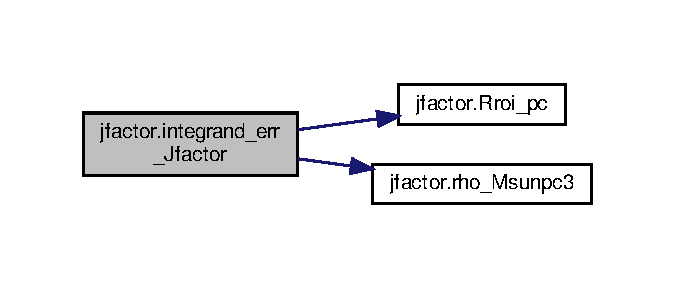
\includegraphics[width=324pt]{de/d47/namespacejfactor_afb33d5b3499565b8b7c23e15f3615ec0_cgraph}
\end{center}
\end{figure}
Here is the caller graph for this function\+:\nopagebreak
\begin{figure}[H]
\begin{center}
\leavevmode
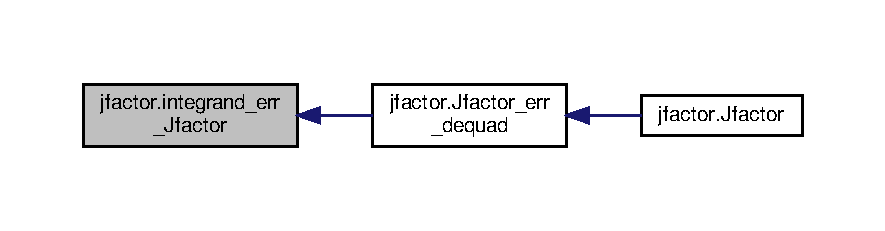
\includegraphics[width=350pt]{de/d47/namespacejfactor_afb33d5b3499565b8b7c23e15f3615ec0_icgraph}
\end{center}
\end{figure}
\mbox{\Hypertarget{namespacejfactor_a3261c30e40781120e1cacf7721893cb7}\label{namespacejfactor_a3261c30e40781120e1cacf7721893cb7}} 
\index{jfactor@{jfactor}!Jfactor@{Jfactor}}
\index{Jfactor@{Jfactor}!jfactor@{jfactor}}
\subsubsection{\texorpdfstring{Jfactor()}{Jfactor()}}
{\footnotesize\ttfamily def jfactor.\+Jfactor (\begin{DoxyParamCaption}\item[{}]{rhos\+\_\+\+Msunpc3,  }\item[{}]{rs\+\_\+pc,  }\item[{}]{a,  }\item[{}]{b,  }\item[{}]{g,  }\item[{}]{dist,  }\item[{}]{Rtrunc\+\_\+pc = {\ttfamily 2000},  }\item[{}]{return\+\_\+relerr = {\ttfamily False},  }\item[{}]{width = {\ttfamily 5e-\/3},  }\item[{}]{pN = {\ttfamily 1000},  }\item[{}]{mN = {\ttfamily 1000},  }\item[{}]{show\+\_\+fig = {\ttfamily False} }\end{DoxyParamCaption})}



Definition at line 84 of file jfactor.\+py.


\begin{DoxyCode}
84 \textcolor{keyword}{def }\hyperlink{namespacejfactor_a3261c30e40781120e1cacf7721893cb7}{Jfactor}(
      rhos\_Msunpc3,rs\_pc,a,b,g,dist,*,Rtrunc\_pc=2000,return\_relerr=False,width=5e-3,pN=1000,mN=1000,show\_fig=False):
85     ret = np.zeros\_like(rhos\_Msunpc3)
86     is\_truncated = Rtrunc\_pc < \hyperlink{namespacejfactor_ae5aad7f2ac90b82740c027677d7f4ac7}{Rroi\_pc}(dist)
87     isnot\_truncated = np.logical\_not(is\_truncated)
88     args\_truncated = [arg[is\_truncated] \textcolor{keywordflow}{for} arg \textcolor{keywordflow}{in} [rhos\_Msunpc3,rs\_pc,a,b,g,dist]]
89     args\_not\_truncated = [arg[isnot\_truncated] \textcolor{keywordflow}{for} arg \textcolor{keywordflow}{in} [rhos\_Msunpc3,rs\_pc,a,b,g,dist]]
90     
91     ret[is\_truncated]  = \hyperlink{namespacejfactor_afd0f5558d89189557900a6a1503261b3}{Jfactor\_v01\_truncated}(*args\_truncated,Rtrunc\_pc)
92     
93     ret\_isnot\_truncated = \hyperlink{namespacejfactor_aeb50ca469052983461a3e8382cfb4f95}{Jfactor\_v01}(*args\_not\_truncated)
94     ret\_isnot\_truncated\_err = \hyperlink{namespacejfactor_a4d9eb98f6dca866cd6248ef6b1c308a5}{Jfactor\_err\_dequad}(*args\_not\_truncated,Rtrunc\_pc=Rtrunc\_pc,
      width=width,pN=pN,mN=mN,show\_fig=show\_fig)
95     ret[isnot\_truncated] = ret\_isnot\_truncated + ret\_isnot\_truncated\_err
96     
97     \textcolor{keywordflow}{return} (ret \textcolor{keywordflow}{if} (\textcolor{keywordflow}{not} return\_relerr) \textcolor{keywordflow}{else} (ret, ret\_isnot\_truncated\_err/ret\_isnot\_truncated) )
98 
99 
100 \textcolor{stringliteral}{'''}
101 \textcolor{stringliteral}{print(np.log10(Jfactor\_v01(np.power(10,-2.05),np.power(10,3.96),2.78,7.78,0.675)))}
102 \textcolor{stringliteral}{print(np.log10(Jfactor\_v02(np.power(10,-2.05),np.power(10,3.96),2.78,7.78,0.675)))}
103 \textcolor{stringliteral}{print(np.log10(Jfactor\_v02(np.power(10,-1.52),np.power(10,3.15),2.77,3.18,0.783)))}
104 \textcolor{stringliteral}{print(np.log10(Jfactor\_v02(np.power(10,-0.497),np.power(10,2.60),1.64,5.29,0.777)))}
105 \textcolor{stringliteral}{quit()}
106 \textcolor{stringliteral}{'''}
107 
\end{DoxyCode}
Here is the call graph for this function\+:\nopagebreak
\begin{figure}[H]
\begin{center}
\leavevmode
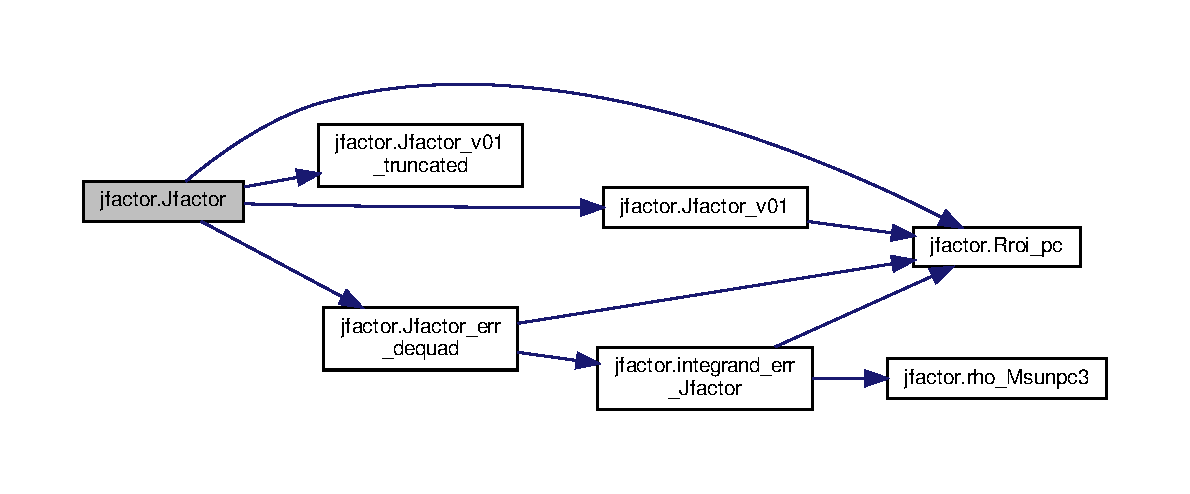
\includegraphics[width=350pt]{de/d47/namespacejfactor_a3261c30e40781120e1cacf7721893cb7_cgraph}
\end{center}
\end{figure}
\mbox{\Hypertarget{namespacejfactor_ad8b8ed7dec1d2c3b4432d37e53117f03}\label{namespacejfactor_ad8b8ed7dec1d2c3b4432d37e53117f03}} 
\index{jfactor@{jfactor}!Jfactor\+\_\+err@{Jfactor\+\_\+err}}
\index{Jfactor\+\_\+err@{Jfactor\+\_\+err}!jfactor@{jfactor}}
\subsubsection{\texorpdfstring{Jfactor\+\_\+err()}{Jfactor\_err()}}
{\footnotesize\ttfamily def jfactor.\+Jfactor\+\_\+err (\begin{DoxyParamCaption}\item[{}]{rhos\+\_\+\+Msunpc3,  }\item[{}]{rs\+\_\+pc,  }\item[{}]{a,  }\item[{}]{b,  }\item[{}]{g,  }\item[{}]{dist,  }\item[{}]{Rtrunc\+\_\+pc = {\ttfamily 2000} }\end{DoxyParamCaption})}



Definition at line 32 of file jfactor.\+py.


\begin{DoxyCode}
32 \textcolor{keyword}{def }\hyperlink{namespacejfactor_ad8b8ed7dec1d2c3b4432d37e53117f03}{Jfactor\_err}(rhos\_Msunpc3,rs\_pc,a,b,g,dist,*,Rtrunc\_pc=2000):
33     integ, err = quad(integrand\_err\_Jfactor,\hyperlink{namespacejfactor_ae5aad7f2ac90b82740c027677d7f4ac7}{Rroi\_pc}(dist),Rtrunc\_pc,args=(rhos\_Msunpc3,rs\_pc,a,b,g,
      dist))
34     \textcolor{keywordflow}{return} C\_J * integ
35 
\end{DoxyCode}
Here is the call graph for this function\+:\nopagebreak
\begin{figure}[H]
\begin{center}
\leavevmode
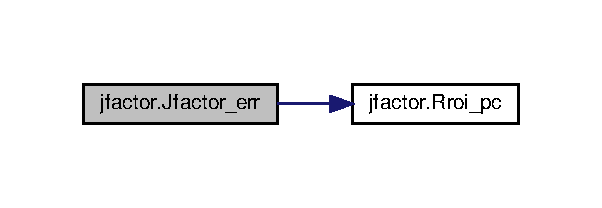
\includegraphics[width=289pt]{de/d47/namespacejfactor_ad8b8ed7dec1d2c3b4432d37e53117f03_cgraph}
\end{center}
\end{figure}
Here is the caller graph for this function\+:\nopagebreak
\begin{figure}[H]
\begin{center}
\leavevmode
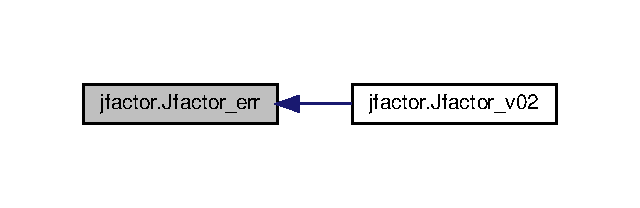
\includegraphics[width=307pt]{de/d47/namespacejfactor_ad8b8ed7dec1d2c3b4432d37e53117f03_icgraph}
\end{center}
\end{figure}
\mbox{\Hypertarget{namespacejfactor_a4d9eb98f6dca866cd6248ef6b1c308a5}\label{namespacejfactor_a4d9eb98f6dca866cd6248ef6b1c308a5}} 
\index{jfactor@{jfactor}!Jfactor\+\_\+err\+\_\+dequad@{Jfactor\+\_\+err\+\_\+dequad}}
\index{Jfactor\+\_\+err\+\_\+dequad@{Jfactor\+\_\+err\+\_\+dequad}!jfactor@{jfactor}}
\subsubsection{\texorpdfstring{Jfactor\+\_\+err\+\_\+dequad()}{Jfactor\_err\_dequad()}}
{\footnotesize\ttfamily def jfactor.\+Jfactor\+\_\+err\+\_\+dequad (\begin{DoxyParamCaption}\item[{}]{rhos\+\_\+\+Msunpc3,  }\item[{}]{rs\+\_\+pc,  }\item[{}]{a,  }\item[{}]{b,  }\item[{}]{g,  }\item[{}]{dist,  }\item[{}]{Rtrunc\+\_\+pc = {\ttfamily 2000},  }\item[{}]{width = {\ttfamily 5e-\/3},  }\item[{}]{pN = {\ttfamily 1000},  }\item[{}]{mN = {\ttfamily 1000},  }\item[{}]{show\+\_\+fig = {\ttfamily True} }\end{DoxyParamCaption})}



Definition at line 36 of file jfactor.\+py.


\begin{DoxyCode}
36 \textcolor{keyword}{def }\hyperlink{namespacejfactor_a4d9eb98f6dca866cd6248ef6b1c308a5}{Jfactor\_err\_dequad}(
      rhos\_Msunpc3,rs\_pc,a,b,g,dist,*,Rtrunc\_pc=2000,width=5e-3,pN=1000,mN=1000,show\_fig=True): 
37     args = [arg[:,np.newaxis] \textcolor{keywordflow}{for} arg \textcolor{keywordflow}{in} [rhos\_Msunpc3,rs\_pc,a,b,g,dist]]
38     func = \textcolor{keyword}{lambda} r\_pc: (Rtrunc\_pc-\hyperlink{namespacejfactor_ae5aad7f2ac90b82740c027677d7f4ac7}{Rroi\_pc}(args[-1]))/2 * 
      \hyperlink{namespacejfactor_afb33d5b3499565b8b7c23e15f3615ec0}{integrand\_err\_Jfactor}((Rtrunc\_pc-\hyperlink{namespacejfactor_ae5aad7f2ac90b82740c027677d7f4ac7}{Rroi\_pc}(args[-1]))/2 * r\_pc + (Rtrunc\_pc+
      \hyperlink{namespacejfactor_ae5aad7f2ac90b82740c027677d7f4ac7}{Rroi\_pc}(args[-1]))/2,*args)
39     integ = \hyperlink{namespacedequad}{dequad}(func,a=-1,b=1,axis=1,ignore\_nan=\textcolor{keyword}{True},show\_fig=show\_fig,width=width,pN=pN,mN=mN)
40     \textcolor{keywordflow}{return} C\_J * integ
41 
\end{DoxyCode}
Here is the call graph for this function\+:\nopagebreak
\begin{figure}[H]
\begin{center}
\leavevmode
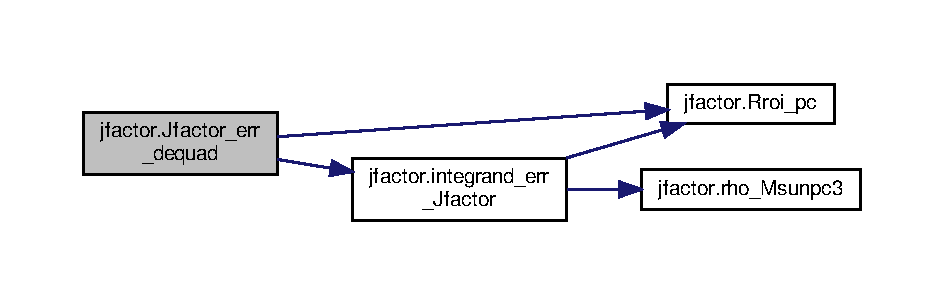
\includegraphics[width=350pt]{de/d47/namespacejfactor_a4d9eb98f6dca866cd6248ef6b1c308a5_cgraph}
\end{center}
\end{figure}
Here is the caller graph for this function\+:\nopagebreak
\begin{figure}[H]
\begin{center}
\leavevmode
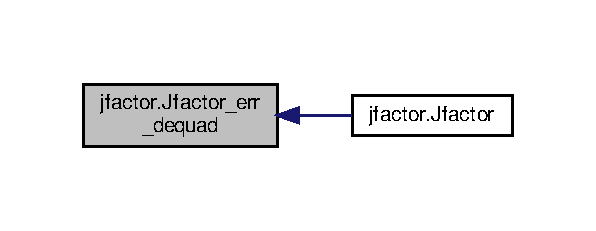
\includegraphics[width=286pt]{de/d47/namespacejfactor_a4d9eb98f6dca866cd6248ef6b1c308a5_icgraph}
\end{center}
\end{figure}
\mbox{\Hypertarget{namespacejfactor_aeb50ca469052983461a3e8382cfb4f95}\label{namespacejfactor_aeb50ca469052983461a3e8382cfb4f95}} 
\index{jfactor@{jfactor}!Jfactor\+\_\+v01@{Jfactor\+\_\+v01}}
\index{Jfactor\+\_\+v01@{Jfactor\+\_\+v01}!jfactor@{jfactor}}
\subsubsection{\texorpdfstring{Jfactor\+\_\+v01()}{Jfactor\_v01()}}
{\footnotesize\ttfamily def jfactor.\+Jfactor\+\_\+v01 (\begin{DoxyParamCaption}\item[{}]{rhos\+\_\+\+Msunpc3,  }\item[{}]{rs\+\_\+pc,  }\item[{}]{a,  }\item[{}]{b,  }\item[{}]{g,  }\item[{}]{dist }\end{DoxyParamCaption})}



Definition at line 42 of file jfactor.\+py.


\begin{DoxyCode}
42 \textcolor{keyword}{def }\hyperlink{namespacejfactor_aeb50ca469052983461a3e8382cfb4f95}{Jfactor\_v01}(rhos\_Msunpc3,rs\_pc,a,b,g,dist):
43     xa = np.power(\hyperlink{namespacejfactor_ae5aad7f2ac90b82740c027677d7f4ac7}{Rroi\_pc}(dist)/rs\_pc,a)
44     argbeta0 = (3.-2.*g)/a
45     argbeta1 = (2.*b-3.)/a
46     argbeta2 = (5.-2.*g)/a
47     argbeta3 = (5.*b-3.)/a
48     \textcolor{keywordflow}{return} C\_J * (
49         (4.*np.pi*rs\_pc**3/a)*rhos\_Msunpc3**2*beta(argbeta0,argbeta1)*betainc(argbeta0,argbeta1,xa/(1+xa))/
      dist**2
50         +(1./3.)*(4.*np.pi*rs\_pc**5/a)*rhos\_Msunpc3**2*beta(argbeta2,argbeta3)*betainc(argbeta2,argbeta3,xa
      /(1+xa))/dist**4
51         ) \textcolor{comment}{#M\_sun/pc^2}
52 
\end{DoxyCode}
Here is the call graph for this function\+:\nopagebreak
\begin{figure}[H]
\begin{center}
\leavevmode
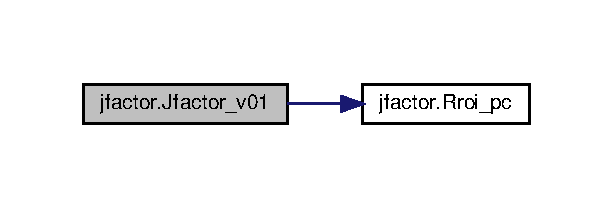
\includegraphics[width=294pt]{de/d47/namespacejfactor_aeb50ca469052983461a3e8382cfb4f95_cgraph}
\end{center}
\end{figure}
Here is the caller graph for this function\+:\nopagebreak
\begin{figure}[H]
\begin{center}
\leavevmode
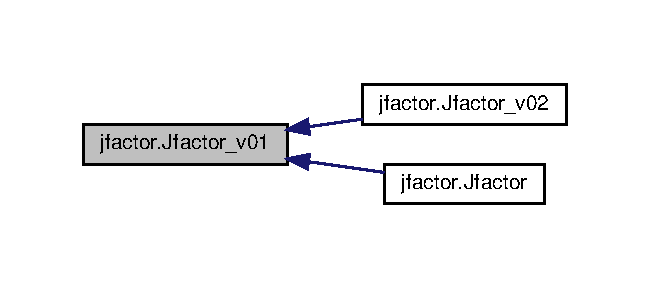
\includegraphics[width=312pt]{de/d47/namespacejfactor_aeb50ca469052983461a3e8382cfb4f95_icgraph}
\end{center}
\end{figure}
\mbox{\Hypertarget{namespacejfactor_afd0f5558d89189557900a6a1503261b3}\label{namespacejfactor_afd0f5558d89189557900a6a1503261b3}} 
\index{jfactor@{jfactor}!Jfactor\+\_\+v01\+\_\+truncated@{Jfactor\+\_\+v01\+\_\+truncated}}
\index{Jfactor\+\_\+v01\+\_\+truncated@{Jfactor\+\_\+v01\+\_\+truncated}!jfactor@{jfactor}}
\subsubsection{\texorpdfstring{Jfactor\+\_\+v01\+\_\+truncated()}{Jfactor\_v01\_truncated()}}
{\footnotesize\ttfamily def jfactor.\+Jfactor\+\_\+v01\+\_\+truncated (\begin{DoxyParamCaption}\item[{}]{rhos\+\_\+\+Msunpc3,  }\item[{}]{rs\+\_\+pc,  }\item[{}]{a,  }\item[{}]{b,  }\item[{}]{g,  }\item[{}]{dist,  }\item[{}]{Rtrunc\+\_\+pc = {\ttfamily 2000} }\end{DoxyParamCaption})}



Definition at line 53 of file jfactor.\+py.


\begin{DoxyCode}
53 \textcolor{keyword}{def }\hyperlink{namespacejfactor_afd0f5558d89189557900a6a1503261b3}{Jfactor\_v01\_truncated}(rhos\_Msunpc3,rs\_pc,a,b,g,dist,Rtrunc\_pc=2000):
54     xa = np.power(Rtrunc\_pc/rs\_pc,a)
55     argbeta0 = (3.-2.*g)/a
56     argbeta1 = (2.*b-3.)/a
57     argbeta2 = (5.-2.*g)/a
58     argbeta3 = (5.*b-3.)/a
59     \textcolor{keywordflow}{return} C\_J * (
60         (4.*np.pi*rs\_pc**3/a)*rhos\_Msunpc3**2*beta(argbeta0,argbeta1)*betainc(argbeta0,argbeta1,xa/(1+xa))/
      dist**2
61         +(1./3.)*(4.*np.pi*rs\_pc**5/a)*rhos\_Msunpc3**2*beta(argbeta2,argbeta3)*betainc(argbeta2,argbeta3,xa
      /(1+xa))/dist**4
62         ) \textcolor{comment}{#M\_sun/pc^2}
63   
64 \textcolor{comment}{#@numba.vectorize(['f8[:](f8[:],f8[:],f8[:],f8[:],f8[:])'])}
65 \textcolor{comment}{#@numba.guvectorize('f8[:](f8[:],f8[:],f8[:],f8[:],f8[:],f8[:])','(m),(m),(m),(m),(m),(m)->(m)')}
\end{DoxyCode}
Here is the caller graph for this function\+:\nopagebreak
\begin{figure}[H]
\begin{center}
\leavevmode
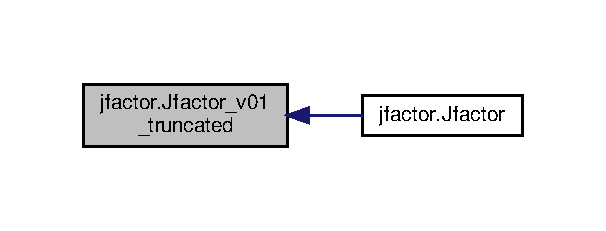
\includegraphics[width=291pt]{de/d47/namespacejfactor_afd0f5558d89189557900a6a1503261b3_icgraph}
\end{center}
\end{figure}
\mbox{\Hypertarget{namespacejfactor_aaa43ebb0d9314fc697123b204465286e}\label{namespacejfactor_aaa43ebb0d9314fc697123b204465286e}} 
\index{jfactor@{jfactor}!Jfactor\+\_\+v02@{Jfactor\+\_\+v02}}
\index{Jfactor\+\_\+v02@{Jfactor\+\_\+v02}!jfactor@{jfactor}}
\subsubsection{\texorpdfstring{Jfactor\+\_\+v02()}{Jfactor\_v02()}}
{\footnotesize\ttfamily def jfactor.\+Jfactor\+\_\+v02 (\begin{DoxyParamCaption}\item[{}]{rhos\+\_\+\+Msunpc3,  }\item[{}]{rs\+\_\+pc,  }\item[{}]{a,  }\item[{}]{b,  }\item[{}]{g,  }\item[{}]{dist,  }\item[{}]{Rtrunc\+\_\+pc = {\ttfamily 2000} }\end{DoxyParamCaption})}



Definition at line 66 of file jfactor.\+py.


\begin{DoxyCode}
66 \textcolor{keyword}{def }\hyperlink{namespacejfactor_aaa43ebb0d9314fc697123b204465286e}{Jfactor\_v02}(rhos\_Msunpc3,rs\_pc,a,b,g,dist,*,Rtrunc\_pc=2000):
67     \textcolor{keywordflow}{if} Rtrunc\_pc < \hyperlink{namespacejfactor_ae5aad7f2ac90b82740c027677d7f4ac7}{Rroi\_pc}(dist):
68         xa = np.power(Rtrunc\_pc/rs\_pc,a)
69         argbeta0 = (3.-2.*g)/a
70         argbeta1 = (2.*b-3.)/a
71         argbeta2 = (5.-2.*g)/a
72         argbeta3 = (5.*b-3.)/a
73         \textcolor{keywordflow}{return} C\_J * (
74             (4.*np.pi*rs\_pc**3/a)*rhos\_Msunpc3**2*beta(argbeta0,argbeta1)*betainc(argbeta0,argbeta1,xa/(1+
      xa))/dist**2
75             +(1./3.)*(4.*np.pi*rs\_pc**5/a)*rhos\_Msunpc3**2*beta(argbeta2,argbeta3)*betainc(argbeta2,
      argbeta3,xa/(1+xa))/dist**4
76             ) \textcolor{comment}{#M\_sun/pc^2}
77     \textcolor{keywordflow}{else}:
78         \textcolor{comment}{#for i in np.arange(rhos\_Msunpc3.shape[0]):}
79         \textcolor{comment}{#    ret[i] = Jfactor\_v01(rhos\_Msunpc3[i],rs\_pc[i],a[i],b[i],g[i]) +
       Jfactor\_err(rhos\_Msunpc3[i],rs\_pc[i],a[i],b[i],g[i])}
80         \textcolor{keywordflow}{return} \hyperlink{namespacejfactor_aeb50ca469052983461a3e8382cfb4f95}{Jfactor\_v01}(rhos\_Msunpc3,rs\_pc,a,b,g,dist) + 
      \hyperlink{namespacejfactor_ad8b8ed7dec1d2c3b4432d37e53117f03}{Jfactor\_err}(rhos\_Msunpc3,rs\_pc,a,b,g,dist=dist,Rtrunc\_pc=Rtrunc\_pc)
81         
\end{DoxyCode}
Here is the call graph for this function\+:\nopagebreak
\begin{figure}[H]
\begin{center}
\leavevmode
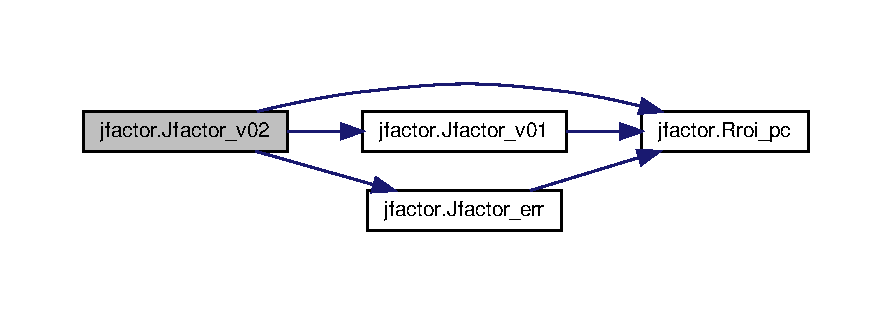
\includegraphics[width=350pt]{de/d47/namespacejfactor_aaa43ebb0d9314fc697123b204465286e_cgraph}
\end{center}
\end{figure}
\mbox{\Hypertarget{namespacejfactor_aa60ca47daf4f993e2cc8bd268f7b206d}\label{namespacejfactor_aa60ca47daf4f993e2cc8bd268f7b206d}} 
\index{jfactor@{jfactor}!rho\+\_\+\+Msunpc3@{rho\+\_\+\+Msunpc3}}
\index{rho\+\_\+\+Msunpc3@{rho\+\_\+\+Msunpc3}!jfactor@{jfactor}}
\subsubsection{\texorpdfstring{rho\+\_\+\+Msunpc3()}{rho\_Msunpc3()}}
{\footnotesize\ttfamily def jfactor.\+rho\+\_\+\+Msunpc3 (\begin{DoxyParamCaption}\item[{}]{r\+\_\+pc,  }\item[{}]{rhos\+\_\+\+Msunpc3,  }\item[{}]{rs\+\_\+pc,  }\item[{}]{a,  }\item[{}]{b,  }\item[{}]{g }\end{DoxyParamCaption})}



Definition at line 24 of file jfactor.\+py.


\begin{DoxyCode}
24 \textcolor{keyword}{def }\hyperlink{namespacejfactor_aa60ca47daf4f993e2cc8bd268f7b206d}{rho\_Msunpc3}(r\_pc,rhos\_Msunpc3,rs\_pc,a,b,g): \textcolor{comment}{#return [Msun]}
25     x = r\_pc/rs\_pc
26     \textcolor{keywordflow}{return} rhos\_Msunpc3*power(x,-g)*power(1+np.power(x,a),-(b-g)/a)
27 
\end{DoxyCode}
Here is the caller graph for this function\+:\nopagebreak
\begin{figure}[H]
\begin{center}
\leavevmode
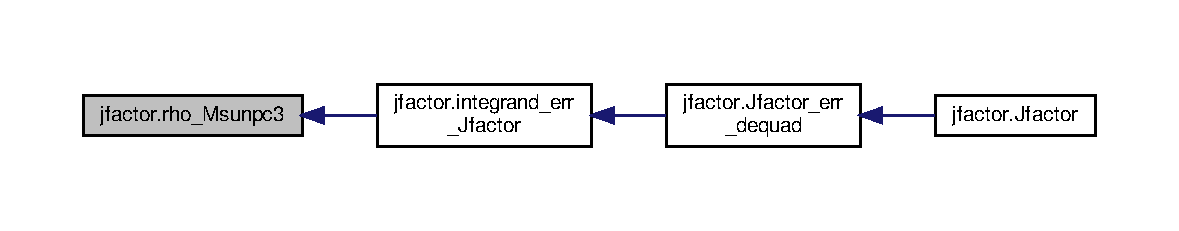
\includegraphics[width=350pt]{de/d47/namespacejfactor_aa60ca47daf4f993e2cc8bd268f7b206d_icgraph}
\end{center}
\end{figure}
\mbox{\Hypertarget{namespacejfactor_ae5aad7f2ac90b82740c027677d7f4ac7}\label{namespacejfactor_ae5aad7f2ac90b82740c027677d7f4ac7}} 
\index{jfactor@{jfactor}!Rroi\+\_\+pc@{Rroi\+\_\+pc}}
\index{Rroi\+\_\+pc@{Rroi\+\_\+pc}!jfactor@{jfactor}}
\subsubsection{\texorpdfstring{Rroi\+\_\+pc()}{Rroi\_pc()}}
{\footnotesize\ttfamily def jfactor.\+Rroi\+\_\+pc (\begin{DoxyParamCaption}\item[{}]{dist }\end{DoxyParamCaption})}



Definition at line 21 of file jfactor.\+py.


\begin{DoxyCode}
21 \textcolor{keyword}{def }\hyperlink{namespacejfactor_ae5aad7f2ac90b82740c027677d7f4ac7}{Rroi\_pc}(dist):
22     \textcolor{keywordflow}{return} dist*np.deg2rad(0.5)
23 
\end{DoxyCode}
Here is the caller graph for this function\+:\nopagebreak
\begin{figure}[H]
\begin{center}
\leavevmode
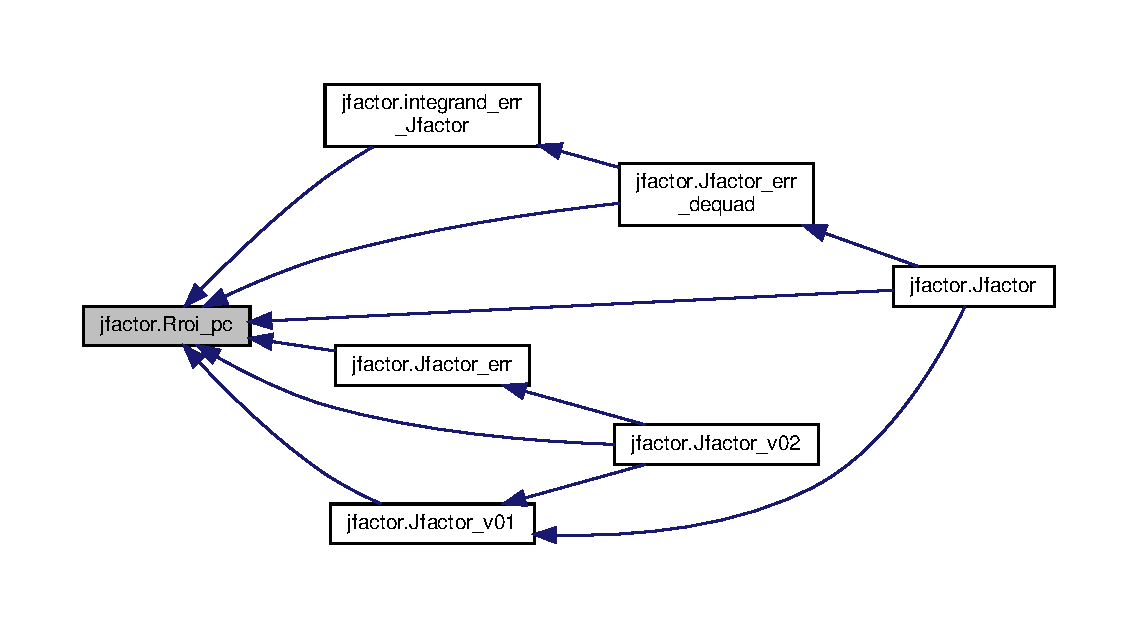
\includegraphics[width=350pt]{de/d47/namespacejfactor_ae5aad7f2ac90b82740c027677d7f4ac7_icgraph}
\end{center}
\end{figure}


\subsection{Variable Documentation}
\mbox{\Hypertarget{namespacejfactor_ab5ce4a1ef962b5f938f157d0abc69a20}\label{namespacejfactor_ab5ce4a1ef962b5f938f157d0abc69a20}} 
\index{jfactor@{jfactor}!a@{a}}
\index{a@{a}!jfactor@{jfactor}}
\subsubsection{\texorpdfstring{a}{a}}
{\footnotesize\ttfamily jfactor.\+a}



Definition at line 131 of file jfactor.\+py.

\mbox{\Hypertarget{namespacejfactor_a7ec02594672c6b2a0a519df5a7648ce2}\label{namespacejfactor_a7ec02594672c6b2a0a519df5a7648ce2}} 
\index{jfactor@{jfactor}!argc@{argc}}
\index{argc@{argc}!jfactor@{jfactor}}
\subsubsection{\texorpdfstring{argc}{argc}}
{\footnotesize\ttfamily jfactor.\+argc = len(\hyperlink{namespacejfactor_a2f38906b89281fb8e6cdc4cbc9c8735e}{argvs})}



Definition at line 111 of file jfactor.\+py.

\mbox{\Hypertarget{namespacejfactor_a2f38906b89281fb8e6cdc4cbc9c8735e}\label{namespacejfactor_a2f38906b89281fb8e6cdc4cbc9c8735e}} 
\index{jfactor@{jfactor}!argvs@{argvs}}
\index{argvs@{argvs}!jfactor@{jfactor}}
\subsubsection{\texorpdfstring{argvs}{argvs}}
{\footnotesize\ttfamily jfactor.\+argvs = sys.\+argv}



Definition at line 110 of file jfactor.\+py.

\mbox{\Hypertarget{namespacejfactor_a768b65ab10ab4bc6a8783ad4fd176789}\label{namespacejfactor_a768b65ab10ab4bc6a8783ad4fd176789}} 
\index{jfactor@{jfactor}!ax@{ax}}
\index{ax@{ax}!jfactor@{jfactor}}
\subsubsection{\texorpdfstring{ax}{ax}}
{\footnotesize\ttfamily jfactor.\+ax = fig.\+add\+\_\+subplot(111)}



Definition at line 158 of file jfactor.\+py.

\mbox{\Hypertarget{namespacejfactor_a52f3e9e591dbe4f5d14f760a578cb15b}\label{namespacejfactor_a52f3e9e591dbe4f5d14f760a578cb15b}} 
\index{jfactor@{jfactor}!b@{b}}
\index{b@{b}!jfactor@{jfactor}}
\subsubsection{\texorpdfstring{b}{b}}
{\footnotesize\ttfamily jfactor.\+b}



Definition at line 131 of file jfactor.\+py.

\mbox{\Hypertarget{namespacejfactor_a819ba1bdb19519796c682583f8b5971f}\label{namespacejfactor_a819ba1bdb19519796c682583f8b5971f}} 
\index{jfactor@{jfactor}!bins@{bins}}
\index{bins@{bins}!jfactor@{jfactor}}
\subsubsection{\texorpdfstring{bins}{bins}}
{\footnotesize\ttfamily jfactor.\+bins}



Definition at line 159 of file jfactor.\+py.

\mbox{\Hypertarget{namespacejfactor_a69776fb72a257bd354abf1104511a3c7}\label{namespacejfactor_a69776fb72a257bd354abf1104511a3c7}} 
\index{jfactor@{jfactor}!C0@{C0}}
\index{C0@{C0}!jfactor@{jfactor}}
\subsubsection{\texorpdfstring{C0}{C0}}
{\footnotesize\ttfamily tuple jfactor.\+C0 = (\hyperlink{namespacejfactor_a30f254edbd584a30535a1b98c2916563}{solar\+\_\+mass\+\_\+kg}$\ast$\hyperlink{namespacejfactor_a2881505111ca34d6a84a5b09a5c19a86}{kg\+\_\+eV})$\ast$$\ast$2$\ast$((1./parsec)$\ast$\hyperlink{namespacejfactor_a3d86861d725265dc096b798369902d43}{im\+\_\+eV})$\ast$$\ast$5}



Definition at line 17 of file jfactor.\+py.

\mbox{\Hypertarget{namespacejfactor_a2c0c80a124f7a32f943f0b9b38f184d4}\label{namespacejfactor_a2c0c80a124f7a32f943f0b9b38f184d4}} 
\index{jfactor@{jfactor}!C1@{C1}}
\index{C1@{C1}!jfactor@{jfactor}}
\subsubsection{\texorpdfstring{C1}{C1}}
{\footnotesize\ttfamily tuple jfactor.\+C1 = (1e9)$\ast$$\ast$2 $\ast$ (1e2$\ast$im\+\_\+e\+V)$\ast$$\ast$5}



Definition at line 18 of file jfactor.\+py.

\mbox{\Hypertarget{namespacejfactor_aaa482b21aae986b864a5adb04d928dab}\label{namespacejfactor_aaa482b21aae986b864a5adb04d928dab}} 
\index{jfactor@{jfactor}!C\+\_\+J@{C\+\_\+J}}
\index{C\+\_\+J@{C\+\_\+J}!jfactor@{jfactor}}
\subsubsection{\texorpdfstring{C\+\_\+J}{C\_J}}
{\footnotesize\ttfamily tuple jfactor.\+C\+\_\+J = \hyperlink{namespacejfactor_a69776fb72a257bd354abf1104511a3c7}{C0}/\hyperlink{namespacejfactor_a2c0c80a124f7a32f943f0b9b38f184d4}{C1}}



Definition at line 19 of file jfactor.\+py.

\mbox{\Hypertarget{namespacejfactor_a543bb58e72396959da8abdb03baad5eb}\label{namespacejfactor_a543bb58e72396959da8abdb03baad5eb}} 
\index{jfactor@{jfactor}!fig@{fig}}
\index{fig@{fig}!jfactor@{jfactor}}
\subsubsection{\texorpdfstring{fig}{fig}}
{\footnotesize\ttfamily jfactor.\+fig = plt.\+figure()}



Definition at line 157 of file jfactor.\+py.

\mbox{\Hypertarget{namespacejfactor_a1e07b351e264fceb00b01b4a591e45e5}\label{namespacejfactor_a1e07b351e264fceb00b01b4a591e45e5}} 
\index{jfactor@{jfactor}!g@{g}}
\index{g@{g}!jfactor@{jfactor}}
\subsubsection{\texorpdfstring{g}{g}}
{\footnotesize\ttfamily jfactor.\+g}



Definition at line 131 of file jfactor.\+py.

\mbox{\Hypertarget{namespacejfactor_a3d86861d725265dc096b798369902d43}\label{namespacejfactor_a3d86861d725265dc096b798369902d43}} 
\index{jfactor@{jfactor}!im\+\_\+eV@{im\+\_\+eV}}
\index{im\+\_\+eV@{im\+\_\+eV}!jfactor@{jfactor}}
\subsubsection{\texorpdfstring{im\+\_\+eV}{im\_eV}}
{\footnotesize\ttfamily int jfactor.\+im\+\_\+eV = 1./physical\+\_\+constants\mbox{[}\char`\"{}electron volt-\/inverse meter relationship\char`\"{}\mbox{]}\mbox{[}0\mbox{]}}



Definition at line 15 of file jfactor.\+py.

\mbox{\Hypertarget{namespacejfactor_a449b6d5eec9600e32c2388268c367957}\label{namespacejfactor_a449b6d5eec9600e32c2388268c367957}} 
\index{jfactor@{jfactor}!ind\+\_\+hi@{ind\+\_\+hi}}
\index{ind\+\_\+hi@{ind\+\_\+hi}!jfactor@{jfactor}}
\subsubsection{\texorpdfstring{ind\+\_\+hi}{ind\_hi}}
{\footnotesize\ttfamily jfactor.\+ind\+\_\+hi = int(\hyperlink{namespacejfactor_a4345d50706cf418a1957595314a7af18}{num}$\ast$0.\+84)}



Definition at line 140 of file jfactor.\+py.

\mbox{\Hypertarget{namespacejfactor_aaf9c1c756ff45c03f48ccc922857360f}\label{namespacejfactor_aaf9c1c756ff45c03f48ccc922857360f}} 
\index{jfactor@{jfactor}!ind\+\_\+lo@{ind\+\_\+lo}}
\index{ind\+\_\+lo@{ind\+\_\+lo}!jfactor@{jfactor}}
\subsubsection{\texorpdfstring{ind\+\_\+lo}{ind\_lo}}
{\footnotesize\ttfamily jfactor.\+ind\+\_\+lo = int(\hyperlink{namespacejfactor_a4345d50706cf418a1957595314a7af18}{num}$\ast$0.\+16)}



Definition at line 139 of file jfactor.\+py.

\mbox{\Hypertarget{namespacejfactor_adfab35ee4763d30c17fe3a8791394e44}\label{namespacejfactor_adfab35ee4763d30c17fe3a8791394e44}} 
\index{jfactor@{jfactor}!Jfactor\+\_\+@{Jfactor\+\_\+}}
\index{Jfactor\+\_\+@{Jfactor\+\_\+}!jfactor@{jfactor}}
\subsubsection{\texorpdfstring{Jfactor\+\_\+}{Jfactor\_}}
{\footnotesize\ttfamily def jfactor.\+Jfactor\+\_\+ = \hyperlink{namespacejfactor_abfd9403bf30810505dc44d7af9746a12}{Jfactor\+\_\+v02}(\hyperlink{namespacejfactor_aa9f6835eba853a5bb2b380ad7fb87010}{rhos\+\_\+\+Msunpc3},\hyperlink{namespacejfactor_ae602db7ab45f472ad4007d04def859f7}{rs\+\_\+pc},\hyperlink{namespacejfactor_ab5ce4a1ef962b5f938f157d0abc69a20}{a},\hyperlink{namespacejfactor_a52f3e9e591dbe4f5d14f760a578cb15b}{b},\hyperlink{namespacejfactor_a1e07b351e264fceb00b01b4a591e45e5}{g})}



Definition at line 136 of file jfactor.\+py.

\mbox{\Hypertarget{namespacejfactor_abfd9403bf30810505dc44d7af9746a12}\label{namespacejfactor_abfd9403bf30810505dc44d7af9746a12}} 
\index{jfactor@{jfactor}!Jfactor\+\_\+v02@{Jfactor\+\_\+v02}}
\index{Jfactor\+\_\+v02@{Jfactor\+\_\+v02}!jfactor@{jfactor}}
\subsubsection{\texorpdfstring{Jfactor\+\_\+v02}{Jfactor\_v02}}
{\footnotesize\ttfamily jfactor.\+Jfactor\+\_\+v02 = np.\+vectorize(Jfactor\+\_\+v02)}



Definition at line 82 of file jfactor.\+py.

\mbox{\Hypertarget{namespacejfactor_a2881505111ca34d6a84a5b09a5c19a86}\label{namespacejfactor_a2881505111ca34d6a84a5b09a5c19a86}} 
\index{jfactor@{jfactor}!kg\+\_\+eV@{kg\+\_\+eV}}
\index{kg\+\_\+eV@{kg\+\_\+eV}!jfactor@{jfactor}}
\subsubsection{\texorpdfstring{kg\+\_\+eV}{kg\_eV}}
{\footnotesize\ttfamily int jfactor.\+kg\+\_\+eV = 1./physical\+\_\+constants\mbox{[}\char`\"{}electron volt-\/kilogram relationship\char`\"{}\mbox{]}\mbox{[}0\mbox{]}}



Definition at line 14 of file jfactor.\+py.

\mbox{\Hypertarget{namespacejfactor_af2c2b0ba5a6685424721abec6152e28d}\label{namespacejfactor_af2c2b0ba5a6685424721abec6152e28d}} 
\index{jfactor@{jfactor}!log10\+\_\+rhos\+\_\+\+Msunpc3@{log10\+\_\+rhos\+\_\+\+Msunpc3}}
\index{log10\+\_\+rhos\+\_\+\+Msunpc3@{log10\+\_\+rhos\+\_\+\+Msunpc3}!jfactor@{jfactor}}
\subsubsection{\texorpdfstring{log10\+\_\+rhos\+\_\+\+Msunpc3}{log10\_rhos\_Msunpc3}}
{\footnotesize\ttfamily jfactor.\+log10\+\_\+rhos\+\_\+\+Msunpc3}



Definition at line 131 of file jfactor.\+py.

\mbox{\Hypertarget{namespacejfactor_a3102b0936ba8da6d8f0bf7044cd1aa7c}\label{namespacejfactor_a3102b0936ba8da6d8f0bf7044cd1aa7c}} 
\index{jfactor@{jfactor}!log10\+\_\+rs\+\_\+pc@{log10\+\_\+rs\+\_\+pc}}
\index{log10\+\_\+rs\+\_\+pc@{log10\+\_\+rs\+\_\+pc}!jfactor@{jfactor}}
\subsubsection{\texorpdfstring{log10\+\_\+rs\+\_\+pc}{log10\_rs\_pc}}
{\footnotesize\ttfamily jfactor.\+log10\+\_\+rs\+\_\+pc}



Definition at line 131 of file jfactor.\+py.

\mbox{\Hypertarget{namespacejfactor_a1e5820e27e0fea1ecb631861940d56c9}\label{namespacejfactor_a1e5820e27e0fea1ecb631861940d56c9}} 
\index{jfactor@{jfactor}!log10\+Jfacotr\+\_\+mean@{log10\+Jfacotr\+\_\+mean}}
\index{log10\+Jfacotr\+\_\+mean@{log10\+Jfacotr\+\_\+mean}!jfactor@{jfactor}}
\subsubsection{\texorpdfstring{log10\+Jfacotr\+\_\+mean}{log10Jfacotr\_mean}}
{\footnotesize\ttfamily jfactor.\+log10\+Jfacotr\+\_\+mean = np.\+mean(\hyperlink{namespacejfactor_a9a89658d06c0c77e0c11e4372ef88f4f}{log10\+Jfactor})}



Definition at line 143 of file jfactor.\+py.

\mbox{\Hypertarget{namespacejfactor_a2d1ea785abc603943b2645a312197359}\label{namespacejfactor_a2d1ea785abc603943b2645a312197359}} 
\index{jfactor@{jfactor}!log10\+Jfacotr\+\_\+median@{log10\+Jfacotr\+\_\+median}}
\index{log10\+Jfacotr\+\_\+median@{log10\+Jfacotr\+\_\+median}!jfactor@{jfactor}}
\subsubsection{\texorpdfstring{log10\+Jfacotr\+\_\+median}{log10Jfacotr\_median}}
{\footnotesize\ttfamily jfactor.\+log10\+Jfacotr\+\_\+median = np.\+median(\hyperlink{namespacejfactor_a9a89658d06c0c77e0c11e4372ef88f4f}{log10\+Jfactor})}



Definition at line 144 of file jfactor.\+py.

\mbox{\Hypertarget{namespacejfactor_a9a89658d06c0c77e0c11e4372ef88f4f}\label{namespacejfactor_a9a89658d06c0c77e0c11e4372ef88f4f}} 
\index{jfactor@{jfactor}!log10\+Jfactor@{log10\+Jfactor}}
\index{log10\+Jfactor@{log10\+Jfactor}!jfactor@{jfactor}}
\subsubsection{\texorpdfstring{log10\+Jfactor}{log10Jfactor}}
{\footnotesize\ttfamily jfactor.\+log10\+Jfactor = np.\+log10(\hyperlink{namespacejfactor_adfab35ee4763d30c17fe3a8791394e44}{Jfactor\+\_\+})}



Definition at line 141 of file jfactor.\+py.

\mbox{\Hypertarget{namespacejfactor_a81a38976b26f5865c633d0d078ab7796}\label{namespacejfactor_a81a38976b26f5865c633d0d078ab7796}} 
\index{jfactor@{jfactor}!log10\+Jfactor\+\_\+sorted@{log10\+Jfactor\+\_\+sorted}}
\index{log10\+Jfactor\+\_\+sorted@{log10\+Jfactor\+\_\+sorted}!jfactor@{jfactor}}
\subsubsection{\texorpdfstring{log10\+Jfactor\+\_\+sorted}{log10Jfactor\_sorted}}
{\footnotesize\ttfamily jfactor.\+log10\+Jfactor\+\_\+sorted = np.\+sort(\hyperlink{namespacejfactor_a9a89658d06c0c77e0c11e4372ef88f4f}{log10\+Jfactor})}



Definition at line 142 of file jfactor.\+py.

\mbox{\Hypertarget{namespacejfactor_a17eab489ecdc2fcda0ff105b820f38a4}\label{namespacejfactor_a17eab489ecdc2fcda0ff105b820f38a4}} 
\index{jfactor@{jfactor}!log10\+Jfactor\+\_\+up@{log10\+Jfactor\+\_\+up}}
\index{log10\+Jfactor\+\_\+up@{log10\+Jfactor\+\_\+up}!jfactor@{jfactor}}
\subsubsection{\texorpdfstring{log10\+Jfactor\+\_\+up}{log10Jfactor\_up}}
{\footnotesize\ttfamily jfactor.\+log10\+Jfactor\+\_\+up = \hyperlink{namespacejfactor_a81a38976b26f5865c633d0d078ab7796}{log10\+Jfactor\+\_\+sorted}\mbox{[}\hyperlink{namespacejfactor_a449b6d5eec9600e32c2388268c367957}{ind\+\_\+hi}\mbox{]}}



Definition at line 146 of file jfactor.\+py.

\mbox{\Hypertarget{namespacejfactor_a9f023e9540cdb0cd16e23b84817d50dd}\label{namespacejfactor_a9f023e9540cdb0cd16e23b84817d50dd}} 
\index{jfactor@{jfactor}!log10\+Jgactor\+\_\+lo@{log10\+Jgactor\+\_\+lo}}
\index{log10\+Jgactor\+\_\+lo@{log10\+Jgactor\+\_\+lo}!jfactor@{jfactor}}
\subsubsection{\texorpdfstring{log10\+Jgactor\+\_\+lo}{log10Jgactor\_lo}}
{\footnotesize\ttfamily jfactor.\+log10\+Jgactor\+\_\+lo = \hyperlink{namespacejfactor_a81a38976b26f5865c633d0d078ab7796}{log10\+Jfactor\+\_\+sorted}\mbox{[}\hyperlink{namespacejfactor_aaf9c1c756ff45c03f48ccc922857360f}{ind\+\_\+lo}\mbox{]}}



Definition at line 145 of file jfactor.\+py.

\mbox{\Hypertarget{namespacejfactor_a1c0eda6de5a29ea1a33584eb69690477}\label{namespacejfactor_a1c0eda6de5a29ea1a33584eb69690477}} 
\index{jfactor@{jfactor}!log\+M\+Cparams@{log\+M\+Cparams}}
\index{log\+M\+Cparams@{log\+M\+Cparams}!jfactor@{jfactor}}
\subsubsection{\texorpdfstring{log\+M\+Cparams}{logMCparams}}
{\footnotesize\ttfamily jfactor.\+log\+M\+Cparams = np.\+concatenate(\hyperlink{namespacejfactor_a025ed272933b6b6f31f688649810e704}{log\+M\+Cparams\+\_\+list}, axis=0)\mbox{[}E\+R\+A\+S\+E\+\_\+\+S\+T\+E\+P\+S\+:,1\+:\mbox{]}}



Definition at line 119 of file jfactor.\+py.

\mbox{\Hypertarget{namespacejfactor_a32ed195f2e906262c560b25bbc440b00}\label{namespacejfactor_a32ed195f2e906262c560b25bbc440b00}} 
\index{jfactor@{jfactor}!log\+M\+Cparams\+\_\+filenames\+\_\+list@{log\+M\+Cparams\+\_\+filenames\+\_\+list}}
\index{log\+M\+Cparams\+\_\+filenames\+\_\+list@{log\+M\+Cparams\+\_\+filenames\+\_\+list}!jfactor@{jfactor}}
\subsubsection{\texorpdfstring{log\+M\+Cparams\+\_\+filenames\+\_\+list}{logMCparams\_filenames\_list}}
{\footnotesize\ttfamily list jfactor.\+log\+M\+Cparams\+\_\+filenames\+\_\+list = \mbox{[}glob.\+glob(argv) for argv in \hyperlink{namespacejfactor_a2f38906b89281fb8e6cdc4cbc9c8735e}{argvs}\mbox{[}1\+:\mbox{]}\mbox{]}}



Definition at line 115 of file jfactor.\+py.

\mbox{\Hypertarget{namespacejfactor_a025ed272933b6b6f31f688649810e704}\label{namespacejfactor_a025ed272933b6b6f31f688649810e704}} 
\index{jfactor@{jfactor}!log\+M\+Cparams\+\_\+list@{log\+M\+Cparams\+\_\+list}}
\index{log\+M\+Cparams\+\_\+list@{log\+M\+Cparams\+\_\+list}!jfactor@{jfactor}}
\subsubsection{\texorpdfstring{log\+M\+Cparams\+\_\+list}{logMCparams\_list}}
{\footnotesize\ttfamily jfactor.\+log\+M\+Cparams\+\_\+list = np.\+array(\mbox{[}np.\+loadtxt(log\+M\+Cparams\+\_\+filename,delimiter=\textquotesingle{},\textquotesingle{},comments=\textquotesingle{}\#\textquotesingle{})\mbox{[}0\+:-\/1,\+:\mbox{]} for log\+M\+Cparams\+\_\+filenames in \hyperlink{namespacejfactor_a32ed195f2e906262c560b25bbc440b00}{log\+M\+Cparams\+\_\+filenames\+\_\+list} for log\+M\+Cparams\+\_\+filename in log\+M\+Cparams\+\_\+filenames\mbox{]})}



Definition at line 116 of file jfactor.\+py.

\mbox{\Hypertarget{namespacejfactor_a4345d50706cf418a1957595314a7af18}\label{namespacejfactor_a4345d50706cf418a1957595314a7af18}} 
\index{jfactor@{jfactor}!num@{num}}
\index{num@{num}!jfactor@{jfactor}}
\subsubsection{\texorpdfstring{num}{num}}
{\footnotesize\ttfamily def jfactor.\+num = Jfactor\+\_\+.\+size}



Definition at line 137 of file jfactor.\+py.

\mbox{\Hypertarget{namespacejfactor_a979d9034e576ba9891d6a8eb13f2a8b9}\label{namespacejfactor_a979d9034e576ba9891d6a8eb13f2a8b9}} 
\index{jfactor@{jfactor}!ploted\+\_\+step@{ploted\+\_\+step}}
\index{ploted\+\_\+step@{ploted\+\_\+step}!jfactor@{jfactor}}
\subsubsection{\texorpdfstring{ploted\+\_\+step}{ploted\_step}}
{\footnotesize\ttfamily jfactor.\+ploted\+\_\+step = log\+M\+Cparams.\+shape\mbox{[}0\mbox{]}}



Definition at line 120 of file jfactor.\+py.

\mbox{\Hypertarget{namespacejfactor_aa9f6835eba853a5bb2b380ad7fb87010}\label{namespacejfactor_aa9f6835eba853a5bb2b380ad7fb87010}} 
\index{jfactor@{jfactor}!rhos\+\_\+\+Msunpc3@{rhos\+\_\+\+Msunpc3}}
\index{rhos\+\_\+\+Msunpc3@{rhos\+\_\+\+Msunpc3}!jfactor@{jfactor}}
\subsubsection{\texorpdfstring{rhos\+\_\+\+Msunpc3}{rhos\_Msunpc3}}
{\footnotesize\ttfamily jfactor.\+rhos\+\_\+\+Msunpc3 = np.\+power(10,\hyperlink{namespacejfactor_af2c2b0ba5a6685424721abec6152e28d}{log10\+\_\+rhos\+\_\+\+Msunpc3})}



Definition at line 132 of file jfactor.\+py.

\mbox{\Hypertarget{namespacejfactor_ae602db7ab45f472ad4007d04def859f7}\label{namespacejfactor_ae602db7ab45f472ad4007d04def859f7}} 
\index{jfactor@{jfactor}!rs\+\_\+pc@{rs\+\_\+pc}}
\index{rs\+\_\+pc@{rs\+\_\+pc}!jfactor@{jfactor}}
\subsubsection{\texorpdfstring{rs\+\_\+pc}{rs\_pc}}
{\footnotesize\ttfamily jfactor.\+rs\+\_\+pc = np.\+power(10,\hyperlink{namespacejfactor_a3102b0936ba8da6d8f0bf7044cd1aa7c}{log10\+\_\+rs\+\_\+pc})}



Definition at line 133 of file jfactor.\+py.

\mbox{\Hypertarget{namespacejfactor_a30f254edbd584a30535a1b98c2916563}\label{namespacejfactor_a30f254edbd584a30535a1b98c2916563}} 
\index{jfactor@{jfactor}!solar\+\_\+mass\+\_\+kg@{solar\+\_\+mass\+\_\+kg}}
\index{solar\+\_\+mass\+\_\+kg@{solar\+\_\+mass\+\_\+kg}!jfactor@{jfactor}}
\subsubsection{\texorpdfstring{solar\+\_\+mass\+\_\+kg}{solar\_mass\_kg}}
{\footnotesize\ttfamily float jfactor.\+solar\+\_\+mass\+\_\+kg = 1.\+9884e30}



Definition at line 16 of file jfactor.\+py.


\hypertarget{namespacemcgenerator}{}\section{mcgenerator Namespace Reference}
\label{namespacemcgenerator}\index{mcgenerator@{mcgenerator}}
\subsection*{Classes}
\begin{DoxyCompactItemize}
\item 
class \hyperlink{classmcgenerator_1_1MCgenerator}{M\+Cgenerator}
\end{DoxyCompactItemize}
\subsection*{Functions}
\begin{DoxyCompactItemize}
\item 
def \hyperlink{namespacemcgenerator_a8f55af530516085f0a5169e130a9b35b}{metropolis\+\_\+generator} (num\+\_\+iter, logpdf\+\_\+func, args\+\_\+logpdf, logpdf\+\_\+value, dargs\+\_\+logpdf, push\+\_\+time=10, proposal\+\_\+dist=\char`\"{}normal\char`\"{}, print\+\_\+func=print)
\end{DoxyCompactItemize}
\subsection*{Variables}
\begin{DoxyCompactItemize}
\item 
int \hyperlink{namespacemcgenerator_a23bb8cafe013a76952e0a2e881d28c5a}{logpdf} = lambda x\+: -\/x$\ast$x/2
\item 
\hyperlink{namespacemcgenerator_aa96e25cd8bcb93136f1b355b2b9fefa8}{gen} = \hyperlink{classmcgenerator_1_1MCgenerator}{M\+Cgenerator}(\hyperlink{namespacemcgenerator_a23bb8cafe013a76952e0a2e881d28c5a}{logpdf},args\+\_\+logpdf\+\_\+init=\{\char`\"{}x\char`\"{}\+:0\},dargs\+\_\+logpdf=\{\char`\"{}x\char`\"{}\+:10\})
\item 
\hyperlink{namespacemcgenerator_a3b26217311f64965e346b0ce0e83680b}{bins}
\end{DoxyCompactItemize}


\subsection{Function Documentation}
\mbox{\Hypertarget{namespacemcgenerator_a8f55af530516085f0a5169e130a9b35b}\label{namespacemcgenerator_a8f55af530516085f0a5169e130a9b35b}} 
\index{mcgenerator@{mcgenerator}!metropolis\+\_\+generator@{metropolis\+\_\+generator}}
\index{metropolis\+\_\+generator@{metropolis\+\_\+generator}!mcgenerator@{mcgenerator}}
\subsubsection{\texorpdfstring{metropolis\+\_\+generator()}{metropolis\_generator()}}
{\footnotesize\ttfamily def mcgenerator.\+metropolis\+\_\+generator (\begin{DoxyParamCaption}\item[{}]{num\+\_\+iter,  }\item[{}]{logpdf\+\_\+func,  }\item[{}]{args\+\_\+logpdf,  }\item[{}]{logpdf\+\_\+value,  }\item[{}]{dargs\+\_\+logpdf,  }\item[{}]{push\+\_\+time = {\ttfamily 10},  }\item[{}]{proposal\+\_\+dist = {\ttfamily \char`\"{}normal\char`\"{}},  }\item[{}]{print\+\_\+func = {\ttfamily print} }\end{DoxyParamCaption})}

\begin{DoxyVerb}E#xplanation: calculate next logpdf by metropolis algorithm
arguments:
    logpdf_value = logpdf_func(**args_logpdf)
    args_logpdf,dargs_logpdf: pd.Series, same index
\end{DoxyVerb}
 

Definition at line 7 of file mcgenerator.\+py.


\begin{DoxyCode}
7 \textcolor{keyword}{def }\hyperlink{namespacemcgenerator_a8f55af530516085f0a5169e130a9b35b}{metropolis\_generator}(
      num\_iter,logpdf\_func,args\_logpdf,logpdf\_value,dargs\_logpdf,push\_time=10,proposal\_dist="normal",print\_func=print):
8     \textcolor{stringliteral}{'''}
9 \textcolor{stringliteral}{    E#xplanation: calculate next logpdf by metropolis algorithm}
10 \textcolor{stringliteral}{    arguments:}
11 \textcolor{stringliteral}{        logpdf\_value = logpdf\_func(**args\_logpdf)}
12 \textcolor{stringliteral}{        args\_logpdf,dargs\_logpdf: pd.Series, same index}
13 \textcolor{stringliteral}{    '''}
14     proposal\_dist\_dic = \{\textcolor{stringliteral}{"normal"}:np.random.normal,\textcolor{stringliteral}{"multivariate\_normal"}:np.random.multivariate\_normal\}
15     proposal\_dist\_func = proposal\_dist\_dic[proposal\_dist]
16     
17     \textcolor{comment}{# initialization}
18     \_args\_logpdf = deepcopy(args\_logpdf)
19     \_logpdf\_value = logpdf\_value
20     \_num\_iter = 0
21     t = time.time()
22     num\_accepted = 0
23 
24     \textcolor{keywordflow}{while} \_num\_iter<num\_iter:
25         args\_logpdf\_candidate = pd.Series(
26             data = proposal\_dist\_func(\_args\_logpdf,dargs\_logpdf),
27             index = \_args\_logpdf.index
28             )
29         logpdf\_value\_candidate = logpdf\_func(**args\_logpdf\_candidate)
30         
31         acceptance\_rate = np.exp(logpdf\_value\_candidate-\_logpdf\_value)
32         
33         \textcolor{keywordflow}{if} np.isnan(acceptance\_rate):
34             mes = \textcolor{stringliteral}{"NaN in acceptance rate calculation at "} + str(\_num\_iter) + \textcolor{stringliteral}{"th calculation \(\backslash\)n"}
35             mes += str(\_logpdf\_value) + \textcolor{stringliteral}{' -> '} + str(logpdf\_value\_candidate) + \textcolor{stringliteral}{'\(\backslash\)n'}
36             mes += \textcolor{stringliteral}{"args\_logpdf:\(\backslash\)n"} + str(\_args\_logpdf) + \textcolor{stringliteral}{'\(\backslash\)n'}
37             mes += \textcolor{stringliteral}{"args\_logpdf\_candidate:\(\backslash\)n"} + str(args\_logpdf\_candidate)
38             \textcolor{keywordflow}{raise} TypeError(mes)
39         
40         \textcolor{keywordflow}{if} np.random.rand() < acceptance\_rate: \textcolor{comment}{# accepted}
41             \textcolor{keywordflow}{yield} \{\textcolor{stringliteral}{"args\_logpdf"}:args\_logpdf\_candidate,\textcolor{stringliteral}{"logpdf\_value"}:logpdf\_value\_candidate\}
42             \_args\_logpdf = args\_logpdf\_candidate
43             \_logpdf\_value = logpdf\_value\_candidate
44             \_num\_iter += 1
45             num\_accepted += 1
46         \textcolor{keywordflow}{else}:
47             \textcolor{keywordflow}{yield} \{\textcolor{stringliteral}{"args\_logpdf"}:\_args\_logpdf,\textcolor{stringliteral}{"logpdf\_value"}:\_logpdf\_value\}
48             \_num\_iter += 1
49         
50         \textcolor{comment}{# for next iteration}
51         dt = time.time() - t
52         \textcolor{keywordflow}{if} dt > push\_time:
53             print(format(\_num\_iter/num\_iter,\textcolor{stringliteral}{".3%"})+\textcolor{stringliteral}{" completed... acceptance rate: "}+ format(num\_accepted/
      \_num\_iter,\textcolor{stringliteral}{'.2%'}))
54             t = time.time()
55 
\end{DoxyCode}
Here is the caller graph for this function\+:\nopagebreak
\begin{figure}[H]
\begin{center}
\leavevmode
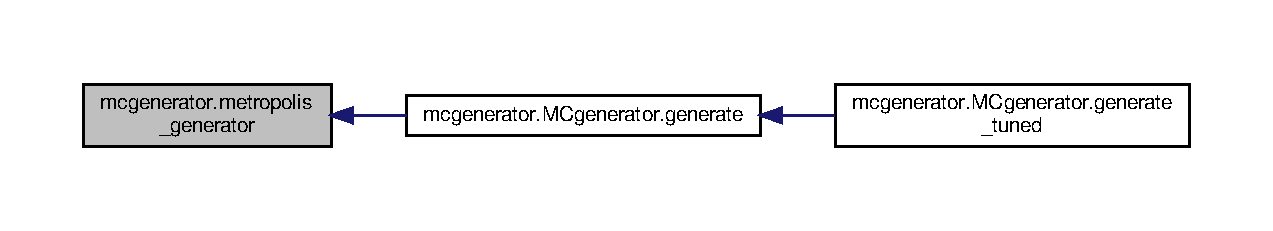
\includegraphics[width=350pt]{d8/daf/namespacemcgenerator_a8f55af530516085f0a5169e130a9b35b_icgraph}
\end{center}
\end{figure}


\subsection{Variable Documentation}
\mbox{\Hypertarget{namespacemcgenerator_a3b26217311f64965e346b0ce0e83680b}\label{namespacemcgenerator_a3b26217311f64965e346b0ce0e83680b}} 
\index{mcgenerator@{mcgenerator}!bins@{bins}}
\index{bins@{bins}!mcgenerator@{mcgenerator}}
\subsubsection{\texorpdfstring{bins}{bins}}
{\footnotesize\ttfamily mcgenerator.\+bins}



Definition at line 233 of file mcgenerator.\+py.

\mbox{\Hypertarget{namespacemcgenerator_aa96e25cd8bcb93136f1b355b2b9fefa8}\label{namespacemcgenerator_aa96e25cd8bcb93136f1b355b2b9fefa8}} 
\index{mcgenerator@{mcgenerator}!gen@{gen}}
\index{gen@{gen}!mcgenerator@{mcgenerator}}
\subsubsection{\texorpdfstring{gen}{gen}}
{\footnotesize\ttfamily mcgenerator.\+gen = \hyperlink{classmcgenerator_1_1MCgenerator}{M\+Cgenerator}(\hyperlink{namespacemcgenerator_a23bb8cafe013a76952e0a2e881d28c5a}{logpdf},args\+\_\+logpdf\+\_\+init=\{\char`\"{}x\char`\"{}\+:0\},dargs\+\_\+logpdf=\{\char`\"{}x\char`\"{}\+:10\})}



Definition at line 228 of file mcgenerator.\+py.

\mbox{\Hypertarget{namespacemcgenerator_a23bb8cafe013a76952e0a2e881d28c5a}\label{namespacemcgenerator_a23bb8cafe013a76952e0a2e881d28c5a}} 
\index{mcgenerator@{mcgenerator}!logpdf@{logpdf}}
\index{logpdf@{logpdf}!mcgenerator@{mcgenerator}}
\subsubsection{\texorpdfstring{logpdf}{logpdf}}
{\footnotesize\ttfamily int mcgenerator.\+logpdf = lambda x\+: -\/x$\ast$x/2}



Definition at line 227 of file mcgenerator.\+py.


\hypertarget{namespacemodki17}{}\section{modki17 Namespace Reference}
\label{namespacemodki17}\index{modki17@{modki17}}
\subsection*{Classes}
\begin{DoxyCompactItemize}
\item 
class \hyperlink{classmodki17_1_1modKI17}{mod\+K\+I17}
\item 
class \hyperlink{classmodki17_1_1modKI17__1gauss}{mod\+K\+I17\+\_\+1gauss}
\item 
class \hyperlink{classmodki17_1_1modKI17__memonly}{mod\+K\+I17\+\_\+memonly}
\item 
class \hyperlink{classmodki17_1_1modKI17__photometry}{mod\+K\+I17\+\_\+photometry}
\end{DoxyCompactItemize}
\subsection*{Functions}
\begin{DoxyCompactItemize}
\item 
def \hyperlink{namespacemodki17_a12f4b9926b321d64b51a76533be122e2}{is\+\_\+positive} (args)
\item 
def \hyperlink{namespacemodki17_ada83ead5e6085ed227b1e64d233eea03}{pow10} (x)
\end{DoxyCompactItemize}
\subsection*{Variables}
\begin{DoxyCompactItemize}
\item 
bool \hyperlink{namespacemodki17_a86807df4fe7d08c11ff4266c9e5dd9ac}{D\+E\+B\+UG} = False
\end{DoxyCompactItemize}


\subsection{Function Documentation}
\mbox{\Hypertarget{namespacemodki17_a12f4b9926b321d64b51a76533be122e2}\label{namespacemodki17_a12f4b9926b321d64b51a76533be122e2}} 
\index{modki17@{modki17}!is\+\_\+positive@{is\+\_\+positive}}
\index{is\+\_\+positive@{is\+\_\+positive}!modki17@{modki17}}
\subsubsection{\texorpdfstring{is\+\_\+positive()}{is\_positive()}}
{\footnotesize\ttfamily def modki17.\+is\+\_\+positive (\begin{DoxyParamCaption}\item[{}]{args }\end{DoxyParamCaption})}



Definition at line 35 of file modki17.\+py.


\begin{DoxyCode}
35 \textcolor{keyword}{def }\hyperlink{namespacemodki17_a12f4b9926b321d64b51a76533be122e2}{is\_positive}(*args):
36     \textcolor{keywordflow}{return} array(args)>0
37 
\end{DoxyCode}
\mbox{\Hypertarget{namespacemodki17_ada83ead5e6085ed227b1e64d233eea03}\label{namespacemodki17_ada83ead5e6085ed227b1e64d233eea03}} 
\index{modki17@{modki17}!pow10@{pow10}}
\index{pow10@{pow10}!modki17@{modki17}}
\subsubsection{\texorpdfstring{pow10()}{pow10()}}
{\footnotesize\ttfamily def modki17.\+pow10 (\begin{DoxyParamCaption}\item[{}]{x }\end{DoxyParamCaption})}



Definition at line 38 of file modki17.\+py.


\begin{DoxyCode}
38 \textcolor{keyword}{def }\hyperlink{namespacemodki17_ada83ead5e6085ed227b1e64d233eea03}{pow10}(x):
39     \textcolor{keywordflow}{return} power(10,x)
40 
\end{DoxyCode}
Here is the caller graph for this function\+:\nopagebreak
\begin{figure}[H]
\begin{center}
\leavevmode
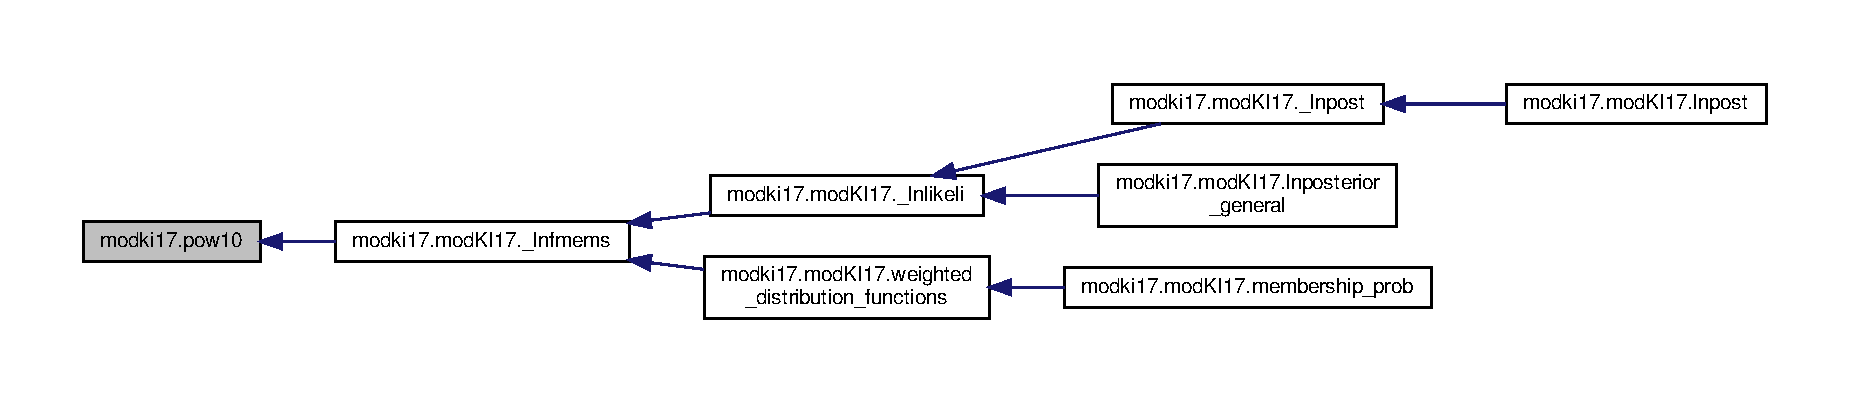
\includegraphics[width=350pt]{db/d4d/namespacemodki17_ada83ead5e6085ed227b1e64d233eea03_icgraph}
\end{center}
\end{figure}


\subsection{Variable Documentation}
\mbox{\Hypertarget{namespacemodki17_a86807df4fe7d08c11ff4266c9e5dd9ac}\label{namespacemodki17_a86807df4fe7d08c11ff4266c9e5dd9ac}} 
\index{modki17@{modki17}!D\+E\+B\+UG@{D\+E\+B\+UG}}
\index{D\+E\+B\+UG@{D\+E\+B\+UG}!modki17@{modki17}}
\subsubsection{\texorpdfstring{D\+E\+B\+UG}{DEBUG}}
{\footnotesize\ttfamily bool modki17.\+D\+E\+B\+UG = False}



Definition at line 23 of file modki17.\+py.


\hypertarget{namespacemodKI17__without__astropy}{}\section{mod\+K\+I17\+\_\+without\+\_\+astropy Namespace Reference}
\label{namespacemodKI17__without__astropy}\index{mod\+K\+I17\+\_\+without\+\_\+astropy@{mod\+K\+I17\+\_\+without\+\_\+astropy}}
\subsection*{Classes}
\begin{DoxyCompactItemize}
\item 
class \hyperlink{classmodKI17__without__astropy_1_1modKI17}{mod\+K\+I17}
\end{DoxyCompactItemize}
\subsection*{Functions}
\begin{DoxyCompactItemize}
\item 
def \hyperlink{namespacemodKI17__without__astropy_a80eeeb18d69cff2fde94fdb26c7c0089}{is\+\_\+positive} (args)
\end{DoxyCompactItemize}
\subsection*{Variables}
\begin{DoxyCompactItemize}
\item 
bool \hyperlink{namespacemodKI17__without__astropy_a9926562322307b1c395c77276b16cb19}{D\+E\+B\+UG} = False
\item 
\hyperlink{namespacemodKI17__without__astropy_a8ee9b076d16981905ef56923bfe9754b}{d\+Sph\+\_\+property} = pd.\+read\+\_\+csv(\char`\"{}d\+Sph\+\_\+property.\+csv\char`\"{},index\+\_\+col=0)
\item 
\hyperlink{namespacemodKI17__without__astropy_a8c61ead2c1a6eb4bd90d556559426eeb}{dsph\+\_\+prop} = d\+Sph\+\_\+property.\+loc\mbox{[}\char`\"{}Sculptor\char`\"{}\mbox{]}
\item 
\hyperlink{namespacemodKI17__without__astropy_a111dd482ab93c59e7e699c09461774bf}{R\+A0} = dsph\+\_\+prop.\+R\+Adeg
\item 
\hyperlink{namespacemodKI17__without__astropy_a20c59be5b70f1194d0996e8582c47eba}{D\+E0} = dsph\+\_\+prop.\+D\+Edeg
\item 
\hyperlink{namespacemodKI17__without__astropy_a94a8ea6dca3b1f107734b2a0312c5087}{D\+I\+ST} = dsph\+\_\+prop.\+D\+I\+ST
\item 
\hyperlink{namespacemodKI17__without__astropy_a891a5d443d2d4949f4d6fc6121650b81}{err\+\_\+\+D\+I\+ST} = dsph\+\_\+prop.\+err\+\_\+\+D\+I\+ST
\end{DoxyCompactItemize}


\subsection{Function Documentation}
\mbox{\Hypertarget{namespacemodKI17__without__astropy_a80eeeb18d69cff2fde94fdb26c7c0089}\label{namespacemodKI17__without__astropy_a80eeeb18d69cff2fde94fdb26c7c0089}} 
\index{mod\+K\+I17\+\_\+without\+\_\+astropy@{mod\+K\+I17\+\_\+without\+\_\+astropy}!is\+\_\+positive@{is\+\_\+positive}}
\index{is\+\_\+positive@{is\+\_\+positive}!mod\+K\+I17\+\_\+without\+\_\+astropy@{mod\+K\+I17\+\_\+without\+\_\+astropy}}
\subsubsection{\texorpdfstring{is\+\_\+positive()}{is\_positive()}}
{\footnotesize\ttfamily def mod\+K\+I17\+\_\+without\+\_\+astropy.\+is\+\_\+positive (\begin{DoxyParamCaption}\item[{}]{args }\end{DoxyParamCaption})}



Definition at line 18 of file mod\+K\+I17\+\_\+without\+\_\+astropy.\+py.


\begin{DoxyCode}
18 \textcolor{keyword}{def }\hyperlink{namespacemodKI17__without__astropy_a80eeeb18d69cff2fde94fdb26c7c0089}{is\_positive}(*args):
19     \textcolor{keywordflow}{return} np.array(args)>0
20 
\end{DoxyCode}


\subsection{Variable Documentation}
\mbox{\Hypertarget{namespacemodKI17__without__astropy_a20c59be5b70f1194d0996e8582c47eba}\label{namespacemodKI17__without__astropy_a20c59be5b70f1194d0996e8582c47eba}} 
\index{mod\+K\+I17\+\_\+without\+\_\+astropy@{mod\+K\+I17\+\_\+without\+\_\+astropy}!D\+E0@{D\+E0}}
\index{D\+E0@{D\+E0}!mod\+K\+I17\+\_\+without\+\_\+astropy@{mod\+K\+I17\+\_\+without\+\_\+astropy}}
\subsubsection{\texorpdfstring{D\+E0}{DE0}}
{\footnotesize\ttfamily mod\+K\+I17\+\_\+without\+\_\+astropy.\+D\+E0 = dsph\+\_\+prop.\+D\+Edeg}



Definition at line 13 of file mod\+K\+I17\+\_\+without\+\_\+astropy.\+py.

\mbox{\Hypertarget{namespacemodKI17__without__astropy_a9926562322307b1c395c77276b16cb19}\label{namespacemodKI17__without__astropy_a9926562322307b1c395c77276b16cb19}} 
\index{mod\+K\+I17\+\_\+without\+\_\+astropy@{mod\+K\+I17\+\_\+without\+\_\+astropy}!D\+E\+B\+UG@{D\+E\+B\+UG}}
\index{D\+E\+B\+UG@{D\+E\+B\+UG}!mod\+K\+I17\+\_\+without\+\_\+astropy@{mod\+K\+I17\+\_\+without\+\_\+astropy}}
\subsubsection{\texorpdfstring{D\+E\+B\+UG}{DEBUG}}
{\footnotesize\ttfamily bool mod\+K\+I17\+\_\+without\+\_\+astropy.\+D\+E\+B\+UG = False}



Definition at line 8 of file mod\+K\+I17\+\_\+without\+\_\+astropy.\+py.

\mbox{\Hypertarget{namespacemodKI17__without__astropy_a94a8ea6dca3b1f107734b2a0312c5087}\label{namespacemodKI17__without__astropy_a94a8ea6dca3b1f107734b2a0312c5087}} 
\index{mod\+K\+I17\+\_\+without\+\_\+astropy@{mod\+K\+I17\+\_\+without\+\_\+astropy}!D\+I\+ST@{D\+I\+ST}}
\index{D\+I\+ST@{D\+I\+ST}!mod\+K\+I17\+\_\+without\+\_\+astropy@{mod\+K\+I17\+\_\+without\+\_\+astropy}}
\subsubsection{\texorpdfstring{D\+I\+ST}{DIST}}
{\footnotesize\ttfamily mod\+K\+I17\+\_\+without\+\_\+astropy.\+D\+I\+ST = dsph\+\_\+prop.\+D\+I\+ST}



Definition at line 14 of file mod\+K\+I17\+\_\+without\+\_\+astropy.\+py.

\mbox{\Hypertarget{namespacemodKI17__without__astropy_a8c61ead2c1a6eb4bd90d556559426eeb}\label{namespacemodKI17__without__astropy_a8c61ead2c1a6eb4bd90d556559426eeb}} 
\index{mod\+K\+I17\+\_\+without\+\_\+astropy@{mod\+K\+I17\+\_\+without\+\_\+astropy}!dsph\+\_\+prop@{dsph\+\_\+prop}}
\index{dsph\+\_\+prop@{dsph\+\_\+prop}!mod\+K\+I17\+\_\+without\+\_\+astropy@{mod\+K\+I17\+\_\+without\+\_\+astropy}}
\subsubsection{\texorpdfstring{dsph\+\_\+prop}{dsph\_prop}}
{\footnotesize\ttfamily mod\+K\+I17\+\_\+without\+\_\+astropy.\+dsph\+\_\+prop = d\+Sph\+\_\+property.\+loc\mbox{[}\char`\"{}Sculptor\char`\"{}\mbox{]}}



Definition at line 11 of file mod\+K\+I17\+\_\+without\+\_\+astropy.\+py.

\mbox{\Hypertarget{namespacemodKI17__without__astropy_a8ee9b076d16981905ef56923bfe9754b}\label{namespacemodKI17__without__astropy_a8ee9b076d16981905ef56923bfe9754b}} 
\index{mod\+K\+I17\+\_\+without\+\_\+astropy@{mod\+K\+I17\+\_\+without\+\_\+astropy}!d\+Sph\+\_\+property@{d\+Sph\+\_\+property}}
\index{d\+Sph\+\_\+property@{d\+Sph\+\_\+property}!mod\+K\+I17\+\_\+without\+\_\+astropy@{mod\+K\+I17\+\_\+without\+\_\+astropy}}
\subsubsection{\texorpdfstring{d\+Sph\+\_\+property}{dSph\_property}}
{\footnotesize\ttfamily mod\+K\+I17\+\_\+without\+\_\+astropy.\+d\+Sph\+\_\+property = pd.\+read\+\_\+csv(\char`\"{}d\+Sph\+\_\+property.\+csv\char`\"{},index\+\_\+col=0)}



Definition at line 10 of file mod\+K\+I17\+\_\+without\+\_\+astropy.\+py.

\mbox{\Hypertarget{namespacemodKI17__without__astropy_a891a5d443d2d4949f4d6fc6121650b81}\label{namespacemodKI17__without__astropy_a891a5d443d2d4949f4d6fc6121650b81}} 
\index{mod\+K\+I17\+\_\+without\+\_\+astropy@{mod\+K\+I17\+\_\+without\+\_\+astropy}!err\+\_\+\+D\+I\+ST@{err\+\_\+\+D\+I\+ST}}
\index{err\+\_\+\+D\+I\+ST@{err\+\_\+\+D\+I\+ST}!mod\+K\+I17\+\_\+without\+\_\+astropy@{mod\+K\+I17\+\_\+without\+\_\+astropy}}
\subsubsection{\texorpdfstring{err\+\_\+\+D\+I\+ST}{err\_DIST}}
{\footnotesize\ttfamily mod\+K\+I17\+\_\+without\+\_\+astropy.\+err\+\_\+\+D\+I\+ST = dsph\+\_\+prop.\+err\+\_\+\+D\+I\+ST}



Definition at line 15 of file mod\+K\+I17\+\_\+without\+\_\+astropy.\+py.

\mbox{\Hypertarget{namespacemodKI17__without__astropy_a111dd482ab93c59e7e699c09461774bf}\label{namespacemodKI17__without__astropy_a111dd482ab93c59e7e699c09461774bf}} 
\index{mod\+K\+I17\+\_\+without\+\_\+astropy@{mod\+K\+I17\+\_\+without\+\_\+astropy}!R\+A0@{R\+A0}}
\index{R\+A0@{R\+A0}!mod\+K\+I17\+\_\+without\+\_\+astropy@{mod\+K\+I17\+\_\+without\+\_\+astropy}}
\subsubsection{\texorpdfstring{R\+A0}{RA0}}
{\footnotesize\ttfamily mod\+K\+I17\+\_\+without\+\_\+astropy.\+R\+A0 = dsph\+\_\+prop.\+R\+Adeg}



Definition at line 12 of file mod\+K\+I17\+\_\+without\+\_\+astropy.\+py.


\hypertarget{namespaceplot__Draco__SDSS__CMD__CMcut}{}\section{plot\+\_\+\+Draco\+\_\+\+S\+D\+S\+S\+\_\+\+C\+M\+D\+\_\+\+C\+Mcut Namespace Reference}
\label{namespaceplot__Draco__SDSS__CMD__CMcut}\index{plot\+\_\+\+Draco\+\_\+\+S\+D\+S\+S\+\_\+\+C\+M\+D\+\_\+\+C\+Mcut@{plot\+\_\+\+Draco\+\_\+\+S\+D\+S\+S\+\_\+\+C\+M\+D\+\_\+\+C\+Mcut}}
\subsection*{Functions}
\begin{DoxyCompactItemize}
\item 
def \hyperlink{namespaceplot__Draco__SDSS__CMD__CMcut_ad99fb273d1ebc75e7b04b98c0a816850}{set\+\_\+axpos\+\_\+coordinates} ()
\begin{DoxyCompactList}\small\item\em def \#\#\#\#\#\#\#\# \end{DoxyCompactList}\item 
def \hyperlink{namespaceplot__Draco__SDSS__CMD__CMcut_a60ce42012054eda79f3b4e90220dabf4}{set\+\_\+axcmd\+\_\+coordinates} ()
\item 
def \hyperlink{namespaceplot__Draco__SDSS__CMD__CMcut_acfc5ebd089fe79d0c0687af77f2fdeb4}{set\+\_\+axpos\+\_\+refference} ()
\item 
def \hyperlink{namespaceplot__Draco__SDSS__CMD__CMcut_aae145b9b27b43700b61a9a20532367a3}{set\+\_\+axcmd\+\_\+refference} ()
\item 
def \hyperlink{namespaceplot__Draco__SDSS__CMD__CMcut_a9bc5b2b68855c01a286faea241fb5940}{slider\+\_\+update} (slider\+\_\+val)
\item 
def \hyperlink{namespaceplot__Draco__SDSS__CMD__CMcut_a476729e1148bad592cbcca8131d3d254}{button\+\_\+clicked} (event)
\item 
def \hyperlink{namespaceplot__Draco__SDSS__CMD__CMcut_accf5e8132b25421b87fac3fde5057644}{onclick} (event)
\end{DoxyCompactItemize}
\subsection*{Variables}
\begin{DoxyCompactItemize}
\item 
string \hyperlink{namespaceplot__Draco__SDSS__CMD__CMcut_a831c14a92a01b5c37b46393599122c71}{I\+M\+P\+O\+R\+T\+\_\+\+S\+D\+S\+S\+\_\+\+F\+I\+L\+E\+N\+A\+ME} = \char`\"{}Draco\+\_\+\+S\+D\+S\+S.\+csv\char`\"{}
\begin{DoxyCompactList}\small\item\em config \#\#\#\#\#\#\#\# \end{DoxyCompactList}\item 
int \hyperlink{namespaceplot__Draco__SDSS__CMD__CMcut_a77aba141d44a10aa841629c09bb35e86}{S\+D\+S\+S\+\_\+\+S\+K\+I\+P\+\_\+\+R\+O\+WS} = 1
\item 
string \hyperlink{namespaceplot__Draco__SDSS__CMD__CMcut_a996b3f27526961cb17360979dbd83065}{C\+M\+D\+\_\+\+P\+L\+O\+T\+\_\+\+T\+I\+T\+LE} = \char`\"{}S\+D\+SS observation of Draco d\+Sph\+: \char`\"{}
\item 
string \hyperlink{namespaceplot__Draco__SDSS__CMD__CMcut_a75199ff0e31b3fc91f5996aecfd3ca0d}{C\+M\+D\+\_\+\+X\+L\+A\+B\+EL} = r\textquotesingle{}\$\hyperlink{namespaceplot__Draco__SDSS__CMD__CMcut_aceb46f1cb6f920499740eb236853cc92}{g}-\/i\$\textquotesingle{}
\item 
string \hyperlink{namespaceplot__Draco__SDSS__CMD__CMcut_a06c22ec66e214aef5832a6f72c5d38c5}{C\+M\+D\+\_\+\+Y\+L\+A\+B\+EL} = r\textquotesingle{}\$i\$\textquotesingle{}
\item 
string \hyperlink{namespaceplot__Draco__SDSS__CMD__CMcut_a3d7fd8c96e93e5e89286d2e3100d11a5}{P\+O\+S\+\_\+\+P\+L\+O\+T\+\_\+\+T\+I\+T\+LE} = \char`\"{}S\+D\+SS observation of Draco\+: posision\char`\"{}
\item 
string \hyperlink{namespaceplot__Draco__SDSS__CMD__CMcut_a0877c5445ed6ac5439ad65bc5deb180d}{E\+X\+P\+O\+R\+T\+\_\+\+F\+I\+L\+E\+N\+A\+ME} = \char`\"{}Draco\+\_\+\+S\+D\+S\+S\+\_\+cut\+\_\+xy\char`\"{}
\item 
string \hyperlink{namespaceplot__Draco__SDSS__CMD__CMcut_ad74a8e00dd2665b433264ecbf8a7a7f5}{E\+X\+P\+O\+R\+T\+\_\+\+F\+I\+L\+E\+N\+A\+M\+E2} = \char`\"{}Draco\+\_\+\+S\+D\+S\+S\+\_\+cut\+\_\+r\char`\"{}
\item 
float \hyperlink{namespaceplot__Draco__SDSS__CMD__CMcut_a47a66344d34ddb1e3eadf4fcb3d12021}{S\+L\+I\+D\+E\+R\+\_\+\+V\+A\+L\+\_\+\+I\+N\+IT} = 1.\+0
\item 
float \hyperlink{namespaceplot__Draco__SDSS__CMD__CMcut_ad39261f3e28c13131eb72d456f3d7233}{S\+L\+I\+D\+E\+R\+\_\+\+V\+A\+L\+\_\+\+M\+AX} = 1.\+5
\item 
float \hyperlink{namespaceplot__Draco__SDSS__CMD__CMcut_ae15a2c2c3ffa4a3b84fc0f5656839de6}{A\+X\+\_\+\+P\+O\+S\+\_\+\+A\+S\+P\+E\+CT} = 0.\+5
\item 
float \hyperlink{namespaceplot__Draco__SDSS__CMD__CMcut_a980cf9f485285e0f42012816f166d695}{A\+X\+\_\+\+P\+O\+S\+\_\+\+X\+R\+A\+N\+GE} = 2.\+1
\item 
float \hyperlink{namespaceplot__Draco__SDSS__CMD__CMcut_a1e8de288a2718587ab6719166ba9959d}{A\+X\+\_\+\+P\+O\+S\+\_\+\+Y\+R\+A\+N\+GE} = \hyperlink{namespaceplot__Draco__SDSS__CMD__CMcut_a980cf9f485285e0f42012816f166d695}{A\+X\+\_\+\+P\+O\+S\+\_\+\+X\+R\+A\+N\+GE}$\ast$\hyperlink{namespaceplot__Draco__SDSS__CMD__CMcut_ae15a2c2c3ffa4a3b84fc0f5656839de6}{A\+X\+\_\+\+P\+O\+S\+\_\+\+A\+S\+P\+E\+CT}
\item 
float \hyperlink{namespaceplot__Draco__SDSS__CMD__CMcut_a0b36091b75b5333bcb2c2b33b515d6e9}{A\+X\+\_\+\+N\+U\+M\+\_\+\+R\+D\+E\+G\+R\+A\+N\+GE} = \hyperlink{namespaceplot__Draco__SDSS__CMD__CMcut_a47a66344d34ddb1e3eadf4fcb3d12021}{S\+L\+I\+D\+E\+R\+\_\+\+V\+A\+L\+\_\+\+I\+N\+IT}
\item 
int \hyperlink{namespaceplot__Draco__SDSS__CMD__CMcut_a3042e57611aacbef7dc04e6cc299a2e8}{A\+X\+\_\+\+N\+U\+M\+\_\+\+B\+I\+N\+N\+UM} = 50
\item 
string \hyperlink{namespaceplot__Draco__SDSS__CMD__CMcut_ad9714a5ae3a136dd47e695a2fafaf2b3}{C\+M\+D\+\_\+\+C\+U\+T\+\_\+\+F\+N\+A\+ME} = \char`\"{}Draco\+\_\+\+C\+M\+Dcut.\+csv\char`\"{}
\item 
\hyperlink{namespaceplot__Draco__SDSS__CMD__CMcut_aa017d84d6f3e9260ccc0bcb5eac49fed}{C\+M\+D\+\_\+\+C\+UT} = np.\+loadtxt(\hyperlink{namespaceplot__Draco__SDSS__CMD__CMcut_ad9714a5ae3a136dd47e695a2fafaf2b3}{C\+M\+D\+\_\+\+C\+U\+T\+\_\+\+F\+N\+A\+ME},delimiter=\char`\"{},\char`\"{})
\item 
\hyperlink{namespaceplot__Draco__SDSS__CMD__CMcut_ab37f89f8fe675c4ab0757fb4a4182a6f}{C\+M\+D\+\_\+\+C\+U\+T\+\_\+C} = np.\+append(\hyperlink{namespaceplot__Draco__SDSS__CMD__CMcut_aa017d84d6f3e9260ccc0bcb5eac49fed}{C\+M\+D\+\_\+\+C\+UT},np.\+array(\mbox{[}\hyperlink{namespaceplot__Draco__SDSS__CMD__CMcut_aa017d84d6f3e9260ccc0bcb5eac49fed}{C\+M\+D\+\_\+\+C\+UT}\mbox{[}0\mbox{]}\mbox{]}),axis=0)
\item 
\hyperlink{namespaceplot__Draco__SDSS__CMD__CMcut_a4cbc86f5f7ecbe01c903e19da60d0f29}{d\+Sph\+\_\+prop} = pd.\+read\+\_\+csv(\char`\"{}d\+Sph\+\_\+property.\+csv\char`\"{},index\+\_\+col=0)
\item 
\hyperlink{namespaceplot__Draco__SDSS__CMD__CMcut_a22c5b1763acfcb31495a03f63f3c6182}{draco\+\_\+prop} = d\+Sph\+\_\+prop.\+loc\mbox{[}\char`\"{}Draco\char`\"{}\mbox{]}
\item 
\hyperlink{namespaceplot__Draco__SDSS__CMD__CMcut_a06b020e30f5517df354b6f8db8d1e22d}{data} = np.\+loadtxt(\hyperlink{namespaceplot__Draco__SDSS__CMD__CMcut_a831c14a92a01b5c37b46393599122c71}{I\+M\+P\+O\+R\+T\+\_\+\+S\+D\+S\+S\+\_\+\+F\+I\+L\+E\+N\+A\+ME},delimiter = \textquotesingle{},\textquotesingle{},skiprows=\hyperlink{namespaceplot__Draco__SDSS__CMD__CMcut_a77aba141d44a10aa841629c09bb35e86}{S\+D\+S\+S\+\_\+\+S\+K\+I\+P\+\_\+\+R\+O\+WS})
\begin{DoxyCompactList}\small\item\em main routin \#\#\#\#\#\#\#\# \end{DoxyCompactList}\item 
\hyperlink{namespaceplot__Draco__SDSS__CMD__CMcut_a455b43c2b64fee5163e0a175c6313229}{pos} = \hyperlink{namespaceplot__Draco__SDSS__CMD__CMcut_a06b020e30f5517df354b6f8db8d1e22d}{data}\mbox{[}\+:,1\+:3\mbox{]}
\begin{DoxyCompactList}\small\item\em split the imported data \#\#\#\# \end{DoxyCompactList}\item 
\hyperlink{namespaceplot__Draco__SDSS__CMD__CMcut_a1d4f3338e366e359d28b436e627317ad}{ra} = \hyperlink{namespaceplot__Draco__SDSS__CMD__CMcut_a455b43c2b64fee5163e0a175c6313229}{pos}\mbox{[}\+:,0\mbox{]}
\item 
\hyperlink{namespaceplot__Draco__SDSS__CMD__CMcut_ac51d42ccd172a5b9e65f9c86aa8db55d}{dec} = \hyperlink{namespaceplot__Draco__SDSS__CMD__CMcut_a455b43c2b64fee5163e0a175c6313229}{pos}\mbox{[}\+:,1\mbox{]}
\item 
\hyperlink{namespaceplot__Draco__SDSS__CMD__CMcut_a7ddace395c7e32e514f063339a1d614f}{g\+\_\+obs} = \hyperlink{namespaceplot__Draco__SDSS__CMD__CMcut_a06b020e30f5517df354b6f8db8d1e22d}{data}\mbox{[}\+:,6\mbox{]}
\item 
\hyperlink{namespaceplot__Draco__SDSS__CMD__CMcut_a98d3e4d508df5a26d2951e5b5e18eb70}{i\+\_\+obs} = \hyperlink{namespaceplot__Draco__SDSS__CMD__CMcut_a06b020e30f5517df354b6f8db8d1e22d}{data}\mbox{[}\+:,8\mbox{]}
\item 
\hyperlink{namespaceplot__Draco__SDSS__CMD__CMcut_ae75c0a2a713511a7807baa4ca817e5be}{g\+\_\+err} = \hyperlink{namespaceplot__Draco__SDSS__CMD__CMcut_a06b020e30f5517df354b6f8db8d1e22d}{data}\mbox{[}\+:,11\mbox{]}
\item 
\hyperlink{namespaceplot__Draco__SDSS__CMD__CMcut_a6b03d439ca243d2617ce6ee0e343eb7a}{i\+\_\+err} = \hyperlink{namespaceplot__Draco__SDSS__CMD__CMcut_a06b020e30f5517df354b6f8db8d1e22d}{data}\mbox{[}\+:,13\mbox{]}
\item 
\hyperlink{namespaceplot__Draco__SDSS__CMD__CMcut_a04000e6eca64ba764e6520de8156462f}{g\+\_\+ext} = \hyperlink{namespaceplot__Draco__SDSS__CMD__CMcut_a06b020e30f5517df354b6f8db8d1e22d}{data}\mbox{[}\+:,16\mbox{]}
\item 
\hyperlink{namespaceplot__Draco__SDSS__CMD__CMcut_a0eced3d157e86dd4cdcb96cc846ee0df}{i\+\_\+ext} = \hyperlink{namespaceplot__Draco__SDSS__CMD__CMcut_a06b020e30f5517df354b6f8db8d1e22d}{data}\mbox{[}\+:,18\mbox{]}
\item 
\hyperlink{namespaceplot__Draco__SDSS__CMD__CMcut_aceb46f1cb6f920499740eb236853cc92}{g} = \hyperlink{namespaceplot__Draco__SDSS__CMD__CMcut_a7ddace395c7e32e514f063339a1d614f}{g\+\_\+obs} -\/ \hyperlink{namespaceplot__Draco__SDSS__CMD__CMcut_a04000e6eca64ba764e6520de8156462f}{g\+\_\+ext}
\item 
\hyperlink{namespaceplot__Draco__SDSS__CMD__CMcut_a6d4ac228accda712923ca1b9740c0407}{i} = \hyperlink{namespaceplot__Draco__SDSS__CMD__CMcut_a98d3e4d508df5a26d2951e5b5e18eb70}{i\+\_\+obs} -\/ \hyperlink{namespaceplot__Draco__SDSS__CMD__CMcut_a0eced3d157e86dd4cdcb96cc846ee0df}{i\+\_\+ext}
\item 
\hyperlink{namespaceplot__Draco__SDSS__CMD__CMcut_a17ecc3c497056424be4f2c1d0fa8a178}{gmi} = \hyperlink{namespaceplot__Draco__SDSS__CMD__CMcut_aceb46f1cb6f920499740eb236853cc92}{g}-\/\hyperlink{namespaceplot__Draco__SDSS__CMD__CMcut_a6d4ac228accda712923ca1b9740c0407}{i}
\item 
\hyperlink{namespaceplot__Draco__SDSS__CMD__CMcut_a67531d4792e3019b4dc270001b538121}{x} = \hyperlink{namespaceplot__Draco__SDSS__CMD__CMcut_a1d4f3338e366e359d28b436e627317ad}{ra} -\/ draco\+\_\+prop.\+R\+Adeg
\item 
\hyperlink{namespaceplot__Draco__SDSS__CMD__CMcut_ad2004cd6fb4127cd926a8619e568255b}{y} = \hyperlink{namespaceplot__Draco__SDSS__CMD__CMcut_ac51d42ccd172a5b9e65f9c86aa8db55d}{dec} -\/ draco\+\_\+prop.\+D\+Edeg
\item 
\hyperlink{namespaceplot__Draco__SDSS__CMD__CMcut_a9fc80a687c10d13188756f83e805ad6e}{xy} = np.\+array(\mbox{[}\hyperlink{namespaceplot__Draco__SDSS__CMD__CMcut_a67531d4792e3019b4dc270001b538121}{x},\hyperlink{namespaceplot__Draco__SDSS__CMD__CMcut_ad2004cd6fb4127cd926a8619e568255b}{y}\mbox{]}).T
\item 
\hyperlink{namespaceplot__Draco__SDSS__CMD__CMcut_af4ccb21831ab318676a2828b7225c1ca}{ind\+\_\+cut} = np.\+where(inpoly(\hyperlink{namespaceplot__Draco__SDSS__CMD__CMcut_a17ecc3c497056424be4f2c1d0fa8a178}{gmi},\hyperlink{namespaceplot__Draco__SDSS__CMD__CMcut_a6d4ac228accda712923ca1b9740c0407}{i},C\+M\+D\+\_\+\+C\+U\+T.\+T\mbox{[}0\mbox{]},C\+M\+D\+\_\+\+C\+U\+T.\+T\mbox{[}1\mbox{]}))
\begin{DoxyCompactList}\small\item\em impose C\+MD cut here \#\#\#\# \end{DoxyCompactList}\item 
\hyperlink{namespaceplot__Draco__SDSS__CMD__CMcut_a08f549437461f522191d2b4d0ea7659f}{coind\+\_\+cut} = np.\+where(np.\+logical\+\_\+not(inpoly(\hyperlink{namespaceplot__Draco__SDSS__CMD__CMcut_a17ecc3c497056424be4f2c1d0fa8a178}{gmi},\hyperlink{namespaceplot__Draco__SDSS__CMD__CMcut_a6d4ac228accda712923ca1b9740c0407}{i},C\+M\+D\+\_\+\+C\+U\+T.\+T\mbox{[}0\mbox{]},C\+M\+D\+\_\+\+C\+U\+T.\+T\mbox{[}1\mbox{]})))
\item 
\hyperlink{namespaceplot__Draco__SDSS__CMD__CMcut_a05465129dacea1fc4a6fedad4b0f0029}{co\+\_\+gmi}
\item 
\hyperlink{namespaceplot__Draco__SDSS__CMD__CMcut_a39d8d2ada3a2e98c5985f134fe54c6ec}{co\+\_\+i}
\item 
\hyperlink{namespaceplot__Draco__SDSS__CMD__CMcut_a4263c5309afa7bc424d494a8f68d69f7}{co\+\_\+x}
\item 
\hyperlink{namespaceplot__Draco__SDSS__CMD__CMcut_a65f19aa6538c710b3afe5b0fe1c4d5df}{co\+\_\+y}
\item 
\hyperlink{namespaceplot__Draco__SDSS__CMD__CMcut_a2e04bc162202f101d86aa8c604ec34c1}{theta} = np.\+arange(360)
\item 
\hyperlink{namespaceplot__Draco__SDSS__CMD__CMcut_a9b33fbee10f744052adb68e2f3bc584e}{hlr\+\_\+ra} = draco\+\_\+prop.\+R\+Adeg$\ast$np.\+cos(np.\+deg2rad(\hyperlink{namespaceplot__Draco__SDSS__CMD__CMcut_a2e04bc162202f101d86aa8c604ec34c1}{theta}))
\item 
\hyperlink{namespaceplot__Draco__SDSS__CMD__CMcut_a50f83d52fd6edd9aa111c67a52423089}{hlr\+\_\+dec} = draco\+\_\+prop.\+D\+Edeg$\ast$np.\+sin(np.\+deg2rad(\hyperlink{namespaceplot__Draco__SDSS__CMD__CMcut_a2e04bc162202f101d86aa8c604ec34c1}{theta}))
\item 
\hyperlink{namespaceplot__Draco__SDSS__CMD__CMcut_afa72503d8c4beee8a7d0855946ddc7a2}{fig} = plt.\+figure()
\begin{DoxyCompactList}\small\item\em plot the data \#\#\#\# \end{DoxyCompactList}\item 
\hyperlink{namespaceplot__Draco__SDSS__CMD__CMcut_ad410368b011d45e4823aaf609922415c}{ax\+\_\+pos} = fig.\+add\+\_\+subplot(2,2,1)
\item 
\hyperlink{namespaceplot__Draco__SDSS__CMD__CMcut_a6024e35ea81cf9c711059ad7e67f6823}{ax\+\_\+cmd} = fig.\+add\+\_\+subplot(2,2,2)
\item 
\hyperlink{namespaceplot__Draco__SDSS__CMD__CMcut_a8ffec3e03ebe5d27c598231b11ac69b0}{ax\+\_\+num} = fig.\+add\+\_\+subplot(2,2,3)
\item 
\hyperlink{namespaceplot__Draco__SDSS__CMD__CMcut_ac1f9327a715f9b40f6f705b226bf6d4e}{pos\+\_\+copathcol} = ax\+\_\+pos.\+scatter(\hyperlink{namespaceplot__Draco__SDSS__CMD__CMcut_a4263c5309afa7bc424d494a8f68d69f7}{co\+\_\+x},\hyperlink{namespaceplot__Draco__SDSS__CMD__CMcut_a65f19aa6538c710b3afe5b0fe1c4d5df}{co\+\_\+y},c=\textquotesingle{}0.\+9\textquotesingle{},s=0.\+1)
\item 
\hyperlink{namespaceplot__Draco__SDSS__CMD__CMcut_a383932c8693f340c6e0befa8ceec8d1c}{pos\+\_\+pathcol} = ax\+\_\+pos.\+scatter(\hyperlink{namespaceplot__Draco__SDSS__CMD__CMcut_a67531d4792e3019b4dc270001b538121}{x},\hyperlink{namespaceplot__Draco__SDSS__CMD__CMcut_ad2004cd6fb4127cd926a8619e568255b}{y},c=\textquotesingle{}gray\textquotesingle{},s=0.\+1)
\item 
\hyperlink{namespaceplot__Draco__SDSS__CMD__CMcut_a7d387739060bb462041d2ec5390a742d}{cmd\+\_\+copathcol} = ax\+\_\+cmd.\+scatter(\hyperlink{namespaceplot__Draco__SDSS__CMD__CMcut_a05465129dacea1fc4a6fedad4b0f0029}{co\+\_\+gmi},\hyperlink{namespaceplot__Draco__SDSS__CMD__CMcut_a39d8d2ada3a2e98c5985f134fe54c6ec}{co\+\_\+i},c=\textquotesingle{}0.\+9\textquotesingle{},s=0.\+1)
\item 
\hyperlink{namespaceplot__Draco__SDSS__CMD__CMcut_aa97847513608fe9d0ea4a87c53872c20}{cmd\+\_\+pathcol} = ax\+\_\+cmd.\+scatter(\hyperlink{namespaceplot__Draco__SDSS__CMD__CMcut_a17ecc3c497056424be4f2c1d0fa8a178}{gmi},\hyperlink{namespaceplot__Draco__SDSS__CMD__CMcut_a6d4ac228accda712923ca1b9740c0407}{i},c=\textquotesingle{}gray\textquotesingle{},s=0.\+1)
\item 
int \hyperlink{namespaceplot__Draco__SDSS__CMD__CMcut_a18d6de36e98130ab16c708346576b80f}{binnum} = 100
\item 
\hyperlink{namespaceplot__Draco__SDSS__CMD__CMcut_a70e4e337d90cea561909f4aba7cd8af2}{edges} = np.\+arange(0.\+00,\hyperlink{namespaceplot__Draco__SDSS__CMD__CMcut_a0b36091b75b5333bcb2c2b33b515d6e9}{A\+X\+\_\+\+N\+U\+M\+\_\+\+R\+D\+E\+G\+R\+A\+N\+GE}+1e-\/8,\+A\+X\+\_\+\+N\+U\+M\+\_\+\+R\+D\+E\+G\+R\+A\+N\+G\+E/\+A\+X\+\_\+\+N\+U\+M\+\_\+\+B\+I\+N\+N\+U\+M)
\item 
tuple \hyperlink{namespaceplot__Draco__SDSS__CMD__CMcut_a10bd1df15af258413e5d0d16afbd3ff4}{edge\+\_\+centers} = (\hyperlink{namespaceplot__Draco__SDSS__CMD__CMcut_a70e4e337d90cea561909f4aba7cd8af2}{edges}\mbox{[}1\+:\mbox{]}+\hyperlink{namespaceplot__Draco__SDSS__CMD__CMcut_a70e4e337d90cea561909f4aba7cd8af2}{edges}\mbox{[}\+:-\/1\mbox{]})/2
\item 
\hyperlink{namespaceplot__Draco__SDSS__CMD__CMcut_ac6f096ee0c5751c15a3a4788f13fc307}{n}
\item 
\hyperlink{namespaceplot__Draco__SDSS__CMD__CMcut_a418e76672a07e876f21993cee46fa0c2}{bins}
\item 
\hyperlink{namespaceplot__Draco__SDSS__CMD__CMcut_a0ea6c66bfb2a3d3569a30378ccbc9550}{patches}
\item 
\hyperlink{namespaceplot__Draco__SDSS__CMD__CMcut_ad93ceb4f047f0acf05e17707f3bcf0e7}{histtype}
\item 
\hyperlink{namespaceplot__Draco__SDSS__CMD__CMcut_a76213cbf7bbd778498512a9abf84642c}{normed}
\item 
\hyperlink{namespaceplot__Draco__SDSS__CMD__CMcut_ae9ea8bdfc2a193b917240b9032824549}{ax\+\_\+ndensity} = fig.\+add\+\_\+subplot(2,2,4)
\item 
\hyperlink{namespaceplot__Draco__SDSS__CMD__CMcut_a2190c9d49488ebea9f4183f66e4720d0}{yerr}
\item 
\hyperlink{namespaceplot__Draco__SDSS__CMD__CMcut_ac09098d64f2f877b850de319b2f90cbd}{fmt}
\item 
\hyperlink{namespaceplot__Draco__SDSS__CMD__CMcut_af21f74f14e5bd8fb8cdc1d4b060f0361}{which}
\item 
\hyperlink{namespaceplot__Draco__SDSS__CMD__CMcut_ab84d6f8e5855eb92875aa98938f791a3}{ax\+\_\+slider} = fig.\+add\+\_\+axes(\mbox{[}0.\+1,0.\+01,0.\+8,0.\+03\mbox{]})
\item 
\hyperlink{namespaceplot__Draco__SDSS__CMD__CMcut_a89c6fffbcf2ec676181b539218612288}{ax\+\_\+button} = fig.\+add\+\_\+axes(\mbox{[}0.\+92,0.\+1,0.\+06,0.\+03\mbox{]})
\item 
\hyperlink{namespaceplot__Draco__SDSS__CMD__CMcut_a60fa9b66f1aaed9979524b6928dd3ab8}{slider} = Slider(\hyperlink{namespaceplot__Draco__SDSS__CMD__CMcut_ab84d6f8e5855eb92875aa98938f791a3}{ax\+\_\+slider},\textquotesingle{}cut radius \mbox{[}deg\mbox{]}\textquotesingle{},0,\hyperlink{namespaceplot__Draco__SDSS__CMD__CMcut_ad39261f3e28c13131eb72d456f3d7233}{S\+L\+I\+D\+E\+R\+\_\+\+V\+A\+L\+\_\+\+M\+AX},valinit=\hyperlink{namespaceplot__Draco__SDSS__CMD__CMcut_a47a66344d34ddb1e3eadf4fcb3d12021}{S\+L\+I\+D\+E\+R\+\_\+\+V\+A\+L\+\_\+\+I\+N\+IT})
\item 
\hyperlink{namespaceplot__Draco__SDSS__CMD__CMcut_a504f89601b402fcd9293b8d4334b638b}{button} = Button(\hyperlink{namespaceplot__Draco__SDSS__CMD__CMcut_a89c6fffbcf2ec676181b539218612288}{ax\+\_\+button},\textquotesingle{}export\textquotesingle{})
\end{DoxyCompactItemize}


\subsection{Function Documentation}
\mbox{\Hypertarget{namespaceplot__Draco__SDSS__CMD__CMcut_a476729e1148bad592cbcca8131d3d254}\label{namespaceplot__Draco__SDSS__CMD__CMcut_a476729e1148bad592cbcca8131d3d254}} 
\index{plot\+\_\+\+Draco\+\_\+\+S\+D\+S\+S\+\_\+\+C\+M\+D\+\_\+\+C\+Mcut@{plot\+\_\+\+Draco\+\_\+\+S\+D\+S\+S\+\_\+\+C\+M\+D\+\_\+\+C\+Mcut}!button\+\_\+clicked@{button\+\_\+clicked}}
\index{button\+\_\+clicked@{button\+\_\+clicked}!plot\+\_\+\+Draco\+\_\+\+S\+D\+S\+S\+\_\+\+C\+M\+D\+\_\+\+C\+Mcut@{plot\+\_\+\+Draco\+\_\+\+S\+D\+S\+S\+\_\+\+C\+M\+D\+\_\+\+C\+Mcut}}
\subsubsection{\texorpdfstring{button\+\_\+clicked()}{button\_clicked()}}
{\footnotesize\ttfamily def plot\+\_\+\+Draco\+\_\+\+S\+D\+S\+S\+\_\+\+C\+M\+D\+\_\+\+C\+Mcut.\+button\+\_\+clicked (\begin{DoxyParamCaption}\item[{}]{event }\end{DoxyParamCaption})}



Definition at line 203 of file plot\+\_\+\+Draco\+\_\+\+S\+D\+S\+S\+\_\+\+C\+M\+D\+\_\+\+C\+Mcut.\+py.


\begin{DoxyCode}
203 \textcolor{keyword}{def }\hyperlink{namespaceplot__Draco__SDSS__CMD__CMcut_a476729e1148bad592cbcca8131d3d254}{button\_clicked}(event):
204     \textcolor{comment}{#print(event)}
205     \textcolor{comment}{#ind\_cut = my.dist2d(xy.T,np.array([0,0]))<slider.val}
206     ind\_cut = \hyperlink{namespacecoord_a04a9b47f67924315930327ed806ee648}{projected\_angle}(draco\_prop.RAdeg,draco\_prop.DEdeg,ra,dec,dtype=\textcolor{stringliteral}{"deg"})<
      slider.val
207     x\_reshaped = x[ind\_cut] \textcolor{comment}{#[:] means the refference}
208     y\_reshaped = y[ind\_cut] \textcolor{comment}{#note that "slider\_update" cannot update the variable x and y inside the
       function.}
209     X = np.array([x\_reshaped,y\_reshaped]).T
210     print(X)
211     print(X.shape)
212     np.savetxt(EXPORT\_FILENAME,X,\textcolor{stringliteral}{'%.6e,%.6e'},delimiter=\textcolor{stringliteral}{","},header=\textcolor{stringliteral}{'x\_cut[deg],y\_cut[deg]'},comments=\textcolor{stringliteral}{'#'})
213     print(EXPORT\_FILENAME,\textcolor{stringliteral}{" is exported"})
214 
215     OUTOF\_CIRCLE\_SUF = \textcolor{stringliteral}{"outof\_"}
216     x\_outof\_circle = x[np.logical\_not(ind\_cut)]
217     y\_outof\_circle = y[np.logical\_not(ind\_cut)]
218     X\_outof\_circle = np.array([x\_outof\_circle,y\_outof\_circle]).T
219     np.savetxt(OUTOF\_CIRCLE\_SUF+EXPORT\_FILENAME,X\_outof\_circle,\textcolor{stringliteral}{'%.6e,%.6e'},delimiter=\textcolor{stringliteral}{','},header=\textcolor{stringliteral}{'
      x\_outof\_circle[deg],y\_outof\_circle[deg]'},comments=\textcolor{stringliteral}{'#'})
220     print(OUTOF\_CIRCLE\_SUF+EXPORT\_FILENAME,\textcolor{stringliteral}{'is exported'})
221 
222     myheader = \textcolor{stringliteral}{'r\_cut[deg]. r\_cut = '}+str(slider.val)
223     \textcolor{comment}{
      #np.savetxt(EXPORT\_FILENAME2,my.dist2d(X.T,np.array([0,0])),'%.6e',delimiter=",",header=myheader,comments='#')}
224     np.savetxt(
225         EXPORT\_FILENAME2,
226         \hyperlink{namespacecoord_a04a9b47f67924315930327ed806ee648}{projected\_angle}(
227             draco\_prop.RAdeg,draco\_prop.DEdeg,x\_reshaped+draco\_prop.RAdeg,y\_reshaped+draco\_prop.DEdeg,dtype
      =\textcolor{stringliteral}{"deg"}
228         ),
229         \textcolor{stringliteral}{'%.6e'},delimiter=\textcolor{stringliteral}{","},header=myheader,comments=\textcolor{stringliteral}{'#'}
230     )
231     \textcolor{comment}{#projected\_angle(draco\_prop.RAdeg,draco\_prop.DEdeg,ra,dec,dtype="deg")}
232     print(EXPORT\_FILENAME2,\textcolor{stringliteral}{" is exported"})
233 
234     myheader = \textcolor{stringliteral}{'r\_cut[deg]. r\_cut = '}+str(slider.val)
235     \textcolor{comment}{
      #np.savetxt(OUTOF\_CIRCLE\_SUF+EXPORT\_FILENAME2,my.dist2d(X\_outof\_circle.T,np.array([0,0])),'%.6e',delimiter=",",header=myheader,comments='#')}
236     np.savetxt(OUTOF\_CIRCLE\_SUF+EXPORT\_FILENAME2,\hyperlink{namespacecoord_a04a9b47f67924315930327ed806ee648}{projected\_angle}(draco\_prop.RAdeg,
      draco\_prop.DEdeg,x\_outof\_circle+draco\_prop.RAdeg,y\_outof\_circle+draco\_prop.DEdeg,dtype=\textcolor{stringliteral}{"deg"}),\textcolor{stringliteral}{'%.6e'},delimiter=\textcolor{stringliteral}{","},
      header=myheader,comments=\textcolor{stringliteral}{'#'})
237     print(OUTOF\_CIRCLE\_SUF+EXPORT\_FILENAME2,\textcolor{stringliteral}{" is exported"})
238 
\end{DoxyCode}
Here is the call graph for this function\+:\nopagebreak
\begin{figure}[H]
\begin{center}
\leavevmode
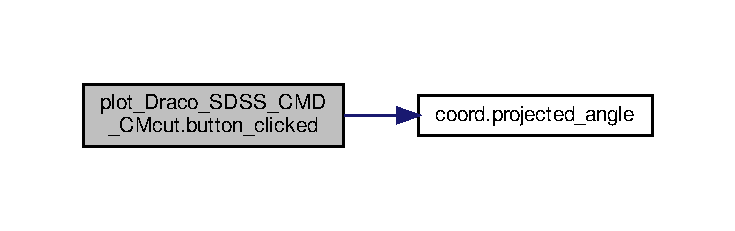
\includegraphics[width=350pt]{d6/dab/namespaceplot__Draco__SDSS__CMD__CMcut_a476729e1148bad592cbcca8131d3d254_cgraph}
\end{center}
\end{figure}
\mbox{\Hypertarget{namespaceplot__Draco__SDSS__CMD__CMcut_accf5e8132b25421b87fac3fde5057644}\label{namespaceplot__Draco__SDSS__CMD__CMcut_accf5e8132b25421b87fac3fde5057644}} 
\index{plot\+\_\+\+Draco\+\_\+\+S\+D\+S\+S\+\_\+\+C\+M\+D\+\_\+\+C\+Mcut@{plot\+\_\+\+Draco\+\_\+\+S\+D\+S\+S\+\_\+\+C\+M\+D\+\_\+\+C\+Mcut}!onclick@{onclick}}
\index{onclick@{onclick}!plot\+\_\+\+Draco\+\_\+\+S\+D\+S\+S\+\_\+\+C\+M\+D\+\_\+\+C\+Mcut@{plot\+\_\+\+Draco\+\_\+\+S\+D\+S\+S\+\_\+\+C\+M\+D\+\_\+\+C\+Mcut}}
\subsubsection{\texorpdfstring{onclick()}{onclick()}}
{\footnotesize\ttfamily def plot\+\_\+\+Draco\+\_\+\+S\+D\+S\+S\+\_\+\+C\+M\+D\+\_\+\+C\+Mcut.\+onclick (\begin{DoxyParamCaption}\item[{}]{event }\end{DoxyParamCaption})}



Definition at line 239 of file plot\+\_\+\+Draco\+\_\+\+S\+D\+S\+S\+\_\+\+C\+M\+D\+\_\+\+C\+Mcut.\+py.


\begin{DoxyCode}
239 \textcolor{keyword}{def }\hyperlink{namespaceplot__Draco__SDSS__CMD__CMcut_accf5e8132b25421b87fac3fde5057644}{onclick}(event):
240     \textcolor{comment}{#print(event)}
241     \textcolor{keywordflow}{if} event.inaxes:
242         \textcolor{keywordflow}{if} event.inaxes!=ax\_slider \textcolor{keywordflow}{and} event.inaxes!=ax\_button:
243             print(\textcolor{stringliteral}{"[x,y]:[%f:%f]"} % (event.xdata,event.ydata))
244 
245 \hyperlink{namespaceplot__Draco__SDSS__CMD__CMcut_a9bc5b2b68855c01a286faea241fb5940}{slider\_update}(SLIDER\_VAL\_INIT) \textcolor{comment}{# initialize}
246 slider.on\_changed(slider\_update)
247 button.on\_clicked(button\_clicked)
248 
249 fig.canvas.mpl\_connect(\textcolor{stringliteral}{'button\_press\_event'},onclick)
250 
251 fig.show()
252 input(\textcolor{stringliteral}{"press any key to exit...\(\backslash\)n"})
253 
254 
255 
256 
257 
258 
259 
260 
261 
262 
263 
264 
265 
266 
267 
268 
269 
270 
271 
272 
273 
274 \end{DoxyCode}
Here is the call graph for this function\+:\nopagebreak
\begin{figure}[H]
\begin{center}
\leavevmode
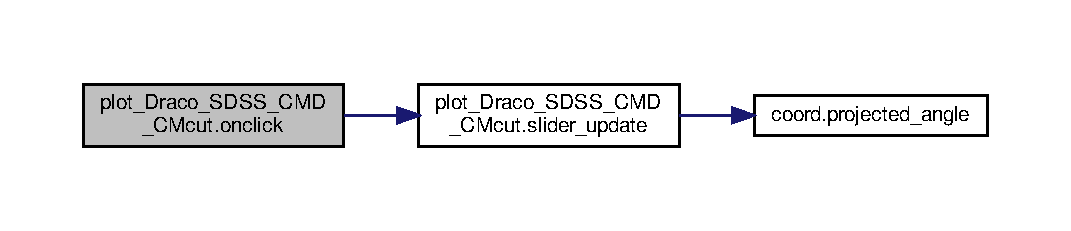
\includegraphics[width=350pt]{d6/dab/namespaceplot__Draco__SDSS__CMD__CMcut_accf5e8132b25421b87fac3fde5057644_cgraph}
\end{center}
\end{figure}
\mbox{\Hypertarget{namespaceplot__Draco__SDSS__CMD__CMcut_a60ce42012054eda79f3b4e90220dabf4}\label{namespaceplot__Draco__SDSS__CMD__CMcut_a60ce42012054eda79f3b4e90220dabf4}} 
\index{plot\+\_\+\+Draco\+\_\+\+S\+D\+S\+S\+\_\+\+C\+M\+D\+\_\+\+C\+Mcut@{plot\+\_\+\+Draco\+\_\+\+S\+D\+S\+S\+\_\+\+C\+M\+D\+\_\+\+C\+Mcut}!set\+\_\+axcmd\+\_\+coordinates@{set\+\_\+axcmd\+\_\+coordinates}}
\index{set\+\_\+axcmd\+\_\+coordinates@{set\+\_\+axcmd\+\_\+coordinates}!plot\+\_\+\+Draco\+\_\+\+S\+D\+S\+S\+\_\+\+C\+M\+D\+\_\+\+C\+Mcut@{plot\+\_\+\+Draco\+\_\+\+S\+D\+S\+S\+\_\+\+C\+M\+D\+\_\+\+C\+Mcut}}
\subsubsection{\texorpdfstring{set\+\_\+axcmd\+\_\+coordinates()}{set\_axcmd\_coordinates()}}
{\footnotesize\ttfamily def plot\+\_\+\+Draco\+\_\+\+S\+D\+S\+S\+\_\+\+C\+M\+D\+\_\+\+C\+Mcut.\+set\+\_\+axcmd\+\_\+coordinates (\begin{DoxyParamCaption}{ }\end{DoxyParamCaption})}



Definition at line 54 of file plot\+\_\+\+Draco\+\_\+\+S\+D\+S\+S\+\_\+\+C\+M\+D\+\_\+\+C\+Mcut.\+py.


\begin{DoxyCode}
54 \textcolor{keyword}{def }\hyperlink{namespaceplot__Draco__SDSS__CMD__CMcut_a60ce42012054eda79f3b4e90220dabf4}{set\_axcmd\_coordinates}():
55     ax\_cmd.set\_title(CMD\_PLOT\_TITLE+IMPORT\_SDSS\_FILENAME)
56     ax\_cmd.set\_xlabel(CMD\_XLABEL) \textcolor{comment}{# "r" before the string means "raw string"}
57     ax\_cmd.set\_ylabel(CMD\_YLABEL) \textcolor{comment}{# we can use TeX format by sandwitching strings with "$"}
58     ax\_cmd.set\_xlim(-0.5,2.5)
59     ax\_cmd.set\_ylim(24,14)
60     ax\_cmd.set\_aspect(0.2)
61 
\end{DoxyCode}
\mbox{\Hypertarget{namespaceplot__Draco__SDSS__CMD__CMcut_aae145b9b27b43700b61a9a20532367a3}\label{namespaceplot__Draco__SDSS__CMD__CMcut_aae145b9b27b43700b61a9a20532367a3}} 
\index{plot\+\_\+\+Draco\+\_\+\+S\+D\+S\+S\+\_\+\+C\+M\+D\+\_\+\+C\+Mcut@{plot\+\_\+\+Draco\+\_\+\+S\+D\+S\+S\+\_\+\+C\+M\+D\+\_\+\+C\+Mcut}!set\+\_\+axcmd\+\_\+refference@{set\+\_\+axcmd\+\_\+refference}}
\index{set\+\_\+axcmd\+\_\+refference@{set\+\_\+axcmd\+\_\+refference}!plot\+\_\+\+Draco\+\_\+\+S\+D\+S\+S\+\_\+\+C\+M\+D\+\_\+\+C\+Mcut@{plot\+\_\+\+Draco\+\_\+\+S\+D\+S\+S\+\_\+\+C\+M\+D\+\_\+\+C\+Mcut}}
\subsubsection{\texorpdfstring{set\+\_\+axcmd\+\_\+refference()}{set\_axcmd\_refference()}}
{\footnotesize\ttfamily def plot\+\_\+\+Draco\+\_\+\+S\+D\+S\+S\+\_\+\+C\+M\+D\+\_\+\+C\+Mcut.\+set\+\_\+axcmd\+\_\+refference (\begin{DoxyParamCaption}{ }\end{DoxyParamCaption})}



Definition at line 66 of file plot\+\_\+\+Draco\+\_\+\+S\+D\+S\+S\+\_\+\+C\+M\+D\+\_\+\+C\+Mcut.\+py.


\begin{DoxyCode}
66 \textcolor{keyword}{def }\hyperlink{namespaceplot__Draco__SDSS__CMD__CMcut_aae145b9b27b43700b61a9a20532367a3}{set\_axcmd\_refference}():
67     ax\_cmd.plot(CMD\_CUT\_C.T[0],CMD\_CUT\_C.T[1])
68 
\end{DoxyCode}
\mbox{\Hypertarget{namespaceplot__Draco__SDSS__CMD__CMcut_ad99fb273d1ebc75e7b04b98c0a816850}\label{namespaceplot__Draco__SDSS__CMD__CMcut_ad99fb273d1ebc75e7b04b98c0a816850}} 
\index{plot\+\_\+\+Draco\+\_\+\+S\+D\+S\+S\+\_\+\+C\+M\+D\+\_\+\+C\+Mcut@{plot\+\_\+\+Draco\+\_\+\+S\+D\+S\+S\+\_\+\+C\+M\+D\+\_\+\+C\+Mcut}!set\+\_\+axpos\+\_\+coordinates@{set\+\_\+axpos\+\_\+coordinates}}
\index{set\+\_\+axpos\+\_\+coordinates@{set\+\_\+axpos\+\_\+coordinates}!plot\+\_\+\+Draco\+\_\+\+S\+D\+S\+S\+\_\+\+C\+M\+D\+\_\+\+C\+Mcut@{plot\+\_\+\+Draco\+\_\+\+S\+D\+S\+S\+\_\+\+C\+M\+D\+\_\+\+C\+Mcut}}
\subsubsection{\texorpdfstring{set\+\_\+axpos\+\_\+coordinates()}{set\_axpos\_coordinates()}}
{\footnotesize\ttfamily def plot\+\_\+\+Draco\+\_\+\+S\+D\+S\+S\+\_\+\+C\+M\+D\+\_\+\+C\+Mcut.\+set\+\_\+axpos\+\_\+coordinates (\begin{DoxyParamCaption}{ }\end{DoxyParamCaption})}



def \#\#\#\#\#\#\#\# 



Definition at line 46 of file plot\+\_\+\+Draco\+\_\+\+S\+D\+S\+S\+\_\+\+C\+M\+D\+\_\+\+C\+Mcut.\+py.


\begin{DoxyCode}
46 \textcolor{keyword}{def }\hyperlink{namespaceplot__Draco__SDSS__CMD__CMcut_ad99fb273d1ebc75e7b04b98c0a816850}{set\_axpos\_coordinates}():
47     ax\_pos.set\_xlabel(\textcolor{stringliteral}{r'$\(\backslash\)xi$[deg]'})
48     ax\_pos.set\_ylabel(\textcolor{stringliteral}{r'$\(\backslash\)eta$[deg]'})
49     ax\_pos.set\_xlim(-AX\_POS\_XRANGE,AX\_POS\_XRANGE)
50     ax\_pos.set\_ylim(-AX\_POS\_YRANGE,AX\_POS\_YRANGE)
51     ax\_pos.set\_title(POS\_PLOT\_TITLE)
52     ax\_pos.set\_aspect(1/AX\_POS\_ASPECT)
53 
\end{DoxyCode}
\mbox{\Hypertarget{namespaceplot__Draco__SDSS__CMD__CMcut_acfc5ebd089fe79d0c0687af77f2fdeb4}\label{namespaceplot__Draco__SDSS__CMD__CMcut_acfc5ebd089fe79d0c0687af77f2fdeb4}} 
\index{plot\+\_\+\+Draco\+\_\+\+S\+D\+S\+S\+\_\+\+C\+M\+D\+\_\+\+C\+Mcut@{plot\+\_\+\+Draco\+\_\+\+S\+D\+S\+S\+\_\+\+C\+M\+D\+\_\+\+C\+Mcut}!set\+\_\+axpos\+\_\+refference@{set\+\_\+axpos\+\_\+refference}}
\index{set\+\_\+axpos\+\_\+refference@{set\+\_\+axpos\+\_\+refference}!plot\+\_\+\+Draco\+\_\+\+S\+D\+S\+S\+\_\+\+C\+M\+D\+\_\+\+C\+Mcut@{plot\+\_\+\+Draco\+\_\+\+S\+D\+S\+S\+\_\+\+C\+M\+D\+\_\+\+C\+Mcut}}
\subsubsection{\texorpdfstring{set\+\_\+axpos\+\_\+refference()}{set\_axpos\_refference()}}
{\footnotesize\ttfamily def plot\+\_\+\+Draco\+\_\+\+S\+D\+S\+S\+\_\+\+C\+M\+D\+\_\+\+C\+Mcut.\+set\+\_\+axpos\+\_\+refference (\begin{DoxyParamCaption}{ }\end{DoxyParamCaption})}



Definition at line 62 of file plot\+\_\+\+Draco\+\_\+\+S\+D\+S\+S\+\_\+\+C\+M\+D\+\_\+\+C\+Mcut.\+py.


\begin{DoxyCode}
62 \textcolor{keyword}{def }\hyperlink{namespaceplot__Draco__SDSS__CMD__CMcut_acfc5ebd089fe79d0c0687af77f2fdeb4}{set\_axpos\_refference}():
63     ax\_pos.scatter(0,0,c=\textcolor{stringliteral}{'red'},s=0.5)
64     ax\_pos.plot(hlr\_ra,hlr\_dec)
65 
\end{DoxyCode}
\mbox{\Hypertarget{namespaceplot__Draco__SDSS__CMD__CMcut_a9bc5b2b68855c01a286faea241fb5940}\label{namespaceplot__Draco__SDSS__CMD__CMcut_a9bc5b2b68855c01a286faea241fb5940}} 
\index{plot\+\_\+\+Draco\+\_\+\+S\+D\+S\+S\+\_\+\+C\+M\+D\+\_\+\+C\+Mcut@{plot\+\_\+\+Draco\+\_\+\+S\+D\+S\+S\+\_\+\+C\+M\+D\+\_\+\+C\+Mcut}!slider\+\_\+update@{slider\+\_\+update}}
\index{slider\+\_\+update@{slider\+\_\+update}!plot\+\_\+\+Draco\+\_\+\+S\+D\+S\+S\+\_\+\+C\+M\+D\+\_\+\+C\+Mcut@{plot\+\_\+\+Draco\+\_\+\+S\+D\+S\+S\+\_\+\+C\+M\+D\+\_\+\+C\+Mcut}}
\subsubsection{\texorpdfstring{slider\+\_\+update()}{slider\_update()}}
{\footnotesize\ttfamily def plot\+\_\+\+Draco\+\_\+\+S\+D\+S\+S\+\_\+\+C\+M\+D\+\_\+\+C\+Mcut.\+slider\+\_\+update (\begin{DoxyParamCaption}\item[{}]{slider\+\_\+val }\end{DoxyParamCaption})}



Definition at line 165 of file plot\+\_\+\+Draco\+\_\+\+S\+D\+S\+S\+\_\+\+C\+M\+D\+\_\+\+C\+Mcut.\+py.


\begin{DoxyCode}
165 \textcolor{keyword}{def }\hyperlink{namespaceplot__Draco__SDSS__CMD__CMcut_a9bc5b2b68855c01a286faea241fb5940}{slider\_update}(slider\_val):
166     \textcolor{comment}{#ax\_pos.clear()  }
167     \textcolor{comment}{#set\_axpos\_coordinates()}
168     \textcolor{comment}{#ind\_cut = projected\_angle(xy.T,np.array([0,0]))<slider\_val}
169     \textcolor{comment}{#ind\_res = my.dist2d(xy.T,np.array([0,0]))>=slider\_val}
170     ind\_cut = \hyperlink{namespacecoord_a04a9b47f67924315930327ed806ee648}{projected\_angle}(draco\_prop.RAdeg,draco\_prop.DEdeg,ra,dec,dtype=\textcolor{stringliteral}{"deg"})<
      slider\_val
171     ind\_res = \hyperlink{namespacecoord_a04a9b47f67924315930327ed806ee648}{projected\_angle}(draco\_prop.RAdeg,draco\_prop.DEdeg,ra,dec,dtype=\textcolor{stringliteral}{"deg"})>=
      slider\_val
172     x\_reshaped = x[ind\_cut] \textcolor{comment}{#[:] means the refference}
173     y\_reshaped = y[ind\_cut]
174     pos\_copathcol.set\_offsets(np.concatenate((np.array([x[ind\_res],y[ind\_res]]).T,np.array([co\_x,co\_y]).T))
      )
175     pos\_pathcol.set\_offsets(np.array([x\_reshaped,y\_reshaped]).T)   
176     \textcolor{comment}{#set\_axpos\_refference()}
177     
178     \textcolor{comment}{#ax\_cmd.clear()}
179     \textcolor{comment}{#set\_axcmd\_coordinates()}
180     gmi\_cut, gmi\_cocut = gmi[ind\_cut], gmi[ind\_res]
181     i\_cut, i\_cocut = i[ind\_cut], i[ind\_res]
182     
183     \textcolor{comment}{#ax\_cmd.scatter(gmi\_cocut,i\_cocut,c='0.9',s=0.1)}
184     cmd\_copathcol.set\_offsets(np.concatenate((np.array([co\_gmi,co\_i]).T,np.array([gmi\_cocut,i\_cocut]).T)))
185     \textcolor{comment}{#ax\_cmd.scatter(co\_gmi,co\_i,c='0.9',s=0.1)}
186     cmd\_pathcol.set\_offsets(np.array([gmi\_cut,i\_cut]).T)
187     \textcolor{comment}{#set\_axcmd\_refference()}
188 
189     ax\_num.clear()
190     edges = np.arange(0.00,AX\_NUM\_RDEGRANGE+1e-8,AX\_NUM\_RDEGRANGE/AX\_NUM\_BINNUM)
191     \textcolor{comment}{
      #ax\_num.hist(my.dist2d(np.array([x\_reshaped,y\_reshaped]),np.array([0,0])),bins=edges,histtype='step',normed=False)}
192     ax\_num.hist(
193         \hyperlink{namespacecoord_a04a9b47f67924315930327ed806ee648}{projected\_angle}(draco\_prop.RAdeg,draco\_prop.DEdeg,x\_reshaped+draco\_prop.RAdeg,
      y\_reshaped+draco\_prop.DEdeg,dtype=\textcolor{stringliteral}{"deg"}),
194         bins=edges,histtype=\textcolor{stringliteral}{'step'},normed=\textcolor{keyword}{False}
195     )
196     \textcolor{comment}{#print(vlos\_pathcol)}
197 
198     fig.canvas.draw()
199     \textcolor{comment}{#fig.show()}
200     \textcolor{comment}{#fig.canvas.flush\_events()}
201     
202 
\end{DoxyCode}
Here is the call graph for this function\+:\nopagebreak
\begin{figure}[H]
\begin{center}
\leavevmode
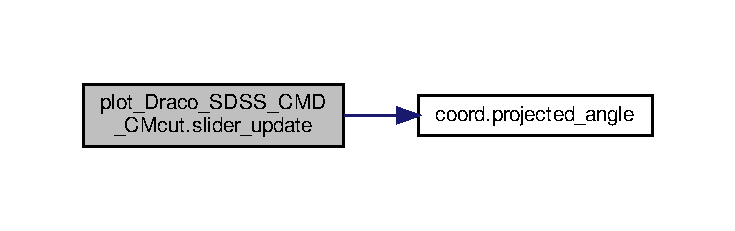
\includegraphics[width=350pt]{d6/dab/namespaceplot__Draco__SDSS__CMD__CMcut_a9bc5b2b68855c01a286faea241fb5940_cgraph}
\end{center}
\end{figure}
Here is the caller graph for this function\+:\nopagebreak
\begin{figure}[H]
\begin{center}
\leavevmode
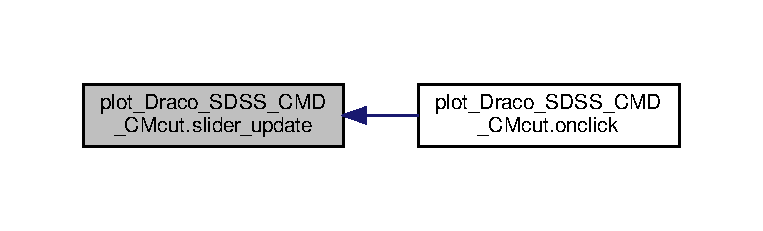
\includegraphics[width=350pt]{d6/dab/namespaceplot__Draco__SDSS__CMD__CMcut_a9bc5b2b68855c01a286faea241fb5940_icgraph}
\end{center}
\end{figure}


\subsection{Variable Documentation}
\mbox{\Hypertarget{namespaceplot__Draco__SDSS__CMD__CMcut_a89c6fffbcf2ec676181b539218612288}\label{namespaceplot__Draco__SDSS__CMD__CMcut_a89c6fffbcf2ec676181b539218612288}} 
\index{plot\+\_\+\+Draco\+\_\+\+S\+D\+S\+S\+\_\+\+C\+M\+D\+\_\+\+C\+Mcut@{plot\+\_\+\+Draco\+\_\+\+S\+D\+S\+S\+\_\+\+C\+M\+D\+\_\+\+C\+Mcut}!ax\+\_\+button@{ax\+\_\+button}}
\index{ax\+\_\+button@{ax\+\_\+button}!plot\+\_\+\+Draco\+\_\+\+S\+D\+S\+S\+\_\+\+C\+M\+D\+\_\+\+C\+Mcut@{plot\+\_\+\+Draco\+\_\+\+S\+D\+S\+S\+\_\+\+C\+M\+D\+\_\+\+C\+Mcut}}
\subsubsection{\texorpdfstring{ax\+\_\+button}{ax\_button}}
{\footnotesize\ttfamily plot\+\_\+\+Draco\+\_\+\+S\+D\+S\+S\+\_\+\+C\+M\+D\+\_\+\+C\+Mcut.\+ax\+\_\+button = fig.\+add\+\_\+axes(\mbox{[}0.\+92,0.\+1,0.\+06,0.\+03\mbox{]})}



Definition at line 161 of file plot\+\_\+\+Draco\+\_\+\+S\+D\+S\+S\+\_\+\+C\+M\+D\+\_\+\+C\+Mcut.\+py.

\mbox{\Hypertarget{namespaceplot__Draco__SDSS__CMD__CMcut_a6024e35ea81cf9c711059ad7e67f6823}\label{namespaceplot__Draco__SDSS__CMD__CMcut_a6024e35ea81cf9c711059ad7e67f6823}} 
\index{plot\+\_\+\+Draco\+\_\+\+S\+D\+S\+S\+\_\+\+C\+M\+D\+\_\+\+C\+Mcut@{plot\+\_\+\+Draco\+\_\+\+S\+D\+S\+S\+\_\+\+C\+M\+D\+\_\+\+C\+Mcut}!ax\+\_\+cmd@{ax\+\_\+cmd}}
\index{ax\+\_\+cmd@{ax\+\_\+cmd}!plot\+\_\+\+Draco\+\_\+\+S\+D\+S\+S\+\_\+\+C\+M\+D\+\_\+\+C\+Mcut@{plot\+\_\+\+Draco\+\_\+\+S\+D\+S\+S\+\_\+\+C\+M\+D\+\_\+\+C\+Mcut}}
\subsubsection{\texorpdfstring{ax\+\_\+cmd}{ax\_cmd}}
{\footnotesize\ttfamily plot\+\_\+\+Draco\+\_\+\+S\+D\+S\+S\+\_\+\+C\+M\+D\+\_\+\+C\+Mcut.\+ax\+\_\+cmd = fig.\+add\+\_\+subplot(2,2,2)}



Definition at line 119 of file plot\+\_\+\+Draco\+\_\+\+S\+D\+S\+S\+\_\+\+C\+M\+D\+\_\+\+C\+Mcut.\+py.

\mbox{\Hypertarget{namespaceplot__Draco__SDSS__CMD__CMcut_ae9ea8bdfc2a193b917240b9032824549}\label{namespaceplot__Draco__SDSS__CMD__CMcut_ae9ea8bdfc2a193b917240b9032824549}} 
\index{plot\+\_\+\+Draco\+\_\+\+S\+D\+S\+S\+\_\+\+C\+M\+D\+\_\+\+C\+Mcut@{plot\+\_\+\+Draco\+\_\+\+S\+D\+S\+S\+\_\+\+C\+M\+D\+\_\+\+C\+Mcut}!ax\+\_\+ndensity@{ax\+\_\+ndensity}}
\index{ax\+\_\+ndensity@{ax\+\_\+ndensity}!plot\+\_\+\+Draco\+\_\+\+S\+D\+S\+S\+\_\+\+C\+M\+D\+\_\+\+C\+Mcut@{plot\+\_\+\+Draco\+\_\+\+S\+D\+S\+S\+\_\+\+C\+M\+D\+\_\+\+C\+Mcut}}
\subsubsection{\texorpdfstring{ax\+\_\+ndensity}{ax\_ndensity}}
{\footnotesize\ttfamily plot\+\_\+\+Draco\+\_\+\+S\+D\+S\+S\+\_\+\+C\+M\+D\+\_\+\+C\+Mcut.\+ax\+\_\+ndensity = fig.\+add\+\_\+subplot(2,2,4)}



Definition at line 145 of file plot\+\_\+\+Draco\+\_\+\+S\+D\+S\+S\+\_\+\+C\+M\+D\+\_\+\+C\+Mcut.\+py.

\mbox{\Hypertarget{namespaceplot__Draco__SDSS__CMD__CMcut_a8ffec3e03ebe5d27c598231b11ac69b0}\label{namespaceplot__Draco__SDSS__CMD__CMcut_a8ffec3e03ebe5d27c598231b11ac69b0}} 
\index{plot\+\_\+\+Draco\+\_\+\+S\+D\+S\+S\+\_\+\+C\+M\+D\+\_\+\+C\+Mcut@{plot\+\_\+\+Draco\+\_\+\+S\+D\+S\+S\+\_\+\+C\+M\+D\+\_\+\+C\+Mcut}!ax\+\_\+num@{ax\+\_\+num}}
\index{ax\+\_\+num@{ax\+\_\+num}!plot\+\_\+\+Draco\+\_\+\+S\+D\+S\+S\+\_\+\+C\+M\+D\+\_\+\+C\+Mcut@{plot\+\_\+\+Draco\+\_\+\+S\+D\+S\+S\+\_\+\+C\+M\+D\+\_\+\+C\+Mcut}}
\subsubsection{\texorpdfstring{ax\+\_\+num}{ax\_num}}
{\footnotesize\ttfamily plot\+\_\+\+Draco\+\_\+\+S\+D\+S\+S\+\_\+\+C\+M\+D\+\_\+\+C\+Mcut.\+ax\+\_\+num = fig.\+add\+\_\+subplot(2,2,3)}



Definition at line 120 of file plot\+\_\+\+Draco\+\_\+\+S\+D\+S\+S\+\_\+\+C\+M\+D\+\_\+\+C\+Mcut.\+py.

\mbox{\Hypertarget{namespaceplot__Draco__SDSS__CMD__CMcut_a3042e57611aacbef7dc04e6cc299a2e8}\label{namespaceplot__Draco__SDSS__CMD__CMcut_a3042e57611aacbef7dc04e6cc299a2e8}} 
\index{plot\+\_\+\+Draco\+\_\+\+S\+D\+S\+S\+\_\+\+C\+M\+D\+\_\+\+C\+Mcut@{plot\+\_\+\+Draco\+\_\+\+S\+D\+S\+S\+\_\+\+C\+M\+D\+\_\+\+C\+Mcut}!A\+X\+\_\+\+N\+U\+M\+\_\+\+B\+I\+N\+N\+UM@{A\+X\+\_\+\+N\+U\+M\+\_\+\+B\+I\+N\+N\+UM}}
\index{A\+X\+\_\+\+N\+U\+M\+\_\+\+B\+I\+N\+N\+UM@{A\+X\+\_\+\+N\+U\+M\+\_\+\+B\+I\+N\+N\+UM}!plot\+\_\+\+Draco\+\_\+\+S\+D\+S\+S\+\_\+\+C\+M\+D\+\_\+\+C\+Mcut@{plot\+\_\+\+Draco\+\_\+\+S\+D\+S\+S\+\_\+\+C\+M\+D\+\_\+\+C\+Mcut}}
\subsubsection{\texorpdfstring{A\+X\+\_\+\+N\+U\+M\+\_\+\+B\+I\+N\+N\+UM}{AX\_NUM\_BINNUM}}
{\footnotesize\ttfamily int plot\+\_\+\+Draco\+\_\+\+S\+D\+S\+S\+\_\+\+C\+M\+D\+\_\+\+C\+Mcut.\+A\+X\+\_\+\+N\+U\+M\+\_\+\+B\+I\+N\+N\+UM = 50}



Definition at line 30 of file plot\+\_\+\+Draco\+\_\+\+S\+D\+S\+S\+\_\+\+C\+M\+D\+\_\+\+C\+Mcut.\+py.

\mbox{\Hypertarget{namespaceplot__Draco__SDSS__CMD__CMcut_a0b36091b75b5333bcb2c2b33b515d6e9}\label{namespaceplot__Draco__SDSS__CMD__CMcut_a0b36091b75b5333bcb2c2b33b515d6e9}} 
\index{plot\+\_\+\+Draco\+\_\+\+S\+D\+S\+S\+\_\+\+C\+M\+D\+\_\+\+C\+Mcut@{plot\+\_\+\+Draco\+\_\+\+S\+D\+S\+S\+\_\+\+C\+M\+D\+\_\+\+C\+Mcut}!A\+X\+\_\+\+N\+U\+M\+\_\+\+R\+D\+E\+G\+R\+A\+N\+GE@{A\+X\+\_\+\+N\+U\+M\+\_\+\+R\+D\+E\+G\+R\+A\+N\+GE}}
\index{A\+X\+\_\+\+N\+U\+M\+\_\+\+R\+D\+E\+G\+R\+A\+N\+GE@{A\+X\+\_\+\+N\+U\+M\+\_\+\+R\+D\+E\+G\+R\+A\+N\+GE}!plot\+\_\+\+Draco\+\_\+\+S\+D\+S\+S\+\_\+\+C\+M\+D\+\_\+\+C\+Mcut@{plot\+\_\+\+Draco\+\_\+\+S\+D\+S\+S\+\_\+\+C\+M\+D\+\_\+\+C\+Mcut}}
\subsubsection{\texorpdfstring{A\+X\+\_\+\+N\+U\+M\+\_\+\+R\+D\+E\+G\+R\+A\+N\+GE}{AX\_NUM\_RDEGRANGE}}
{\footnotesize\ttfamily float plot\+\_\+\+Draco\+\_\+\+S\+D\+S\+S\+\_\+\+C\+M\+D\+\_\+\+C\+Mcut.\+A\+X\+\_\+\+N\+U\+M\+\_\+\+R\+D\+E\+G\+R\+A\+N\+GE = \hyperlink{namespaceplot__Draco__SDSS__CMD__CMcut_a47a66344d34ddb1e3eadf4fcb3d12021}{S\+L\+I\+D\+E\+R\+\_\+\+V\+A\+L\+\_\+\+I\+N\+IT}}



Definition at line 29 of file plot\+\_\+\+Draco\+\_\+\+S\+D\+S\+S\+\_\+\+C\+M\+D\+\_\+\+C\+Mcut.\+py.

\mbox{\Hypertarget{namespaceplot__Draco__SDSS__CMD__CMcut_ad410368b011d45e4823aaf609922415c}\label{namespaceplot__Draco__SDSS__CMD__CMcut_ad410368b011d45e4823aaf609922415c}} 
\index{plot\+\_\+\+Draco\+\_\+\+S\+D\+S\+S\+\_\+\+C\+M\+D\+\_\+\+C\+Mcut@{plot\+\_\+\+Draco\+\_\+\+S\+D\+S\+S\+\_\+\+C\+M\+D\+\_\+\+C\+Mcut}!ax\+\_\+pos@{ax\+\_\+pos}}
\index{ax\+\_\+pos@{ax\+\_\+pos}!plot\+\_\+\+Draco\+\_\+\+S\+D\+S\+S\+\_\+\+C\+M\+D\+\_\+\+C\+Mcut@{plot\+\_\+\+Draco\+\_\+\+S\+D\+S\+S\+\_\+\+C\+M\+D\+\_\+\+C\+Mcut}}
\subsubsection{\texorpdfstring{ax\+\_\+pos}{ax\_pos}}
{\footnotesize\ttfamily plot\+\_\+\+Draco\+\_\+\+S\+D\+S\+S\+\_\+\+C\+M\+D\+\_\+\+C\+Mcut.\+ax\+\_\+pos = fig.\+add\+\_\+subplot(2,2,1)}



Definition at line 118 of file plot\+\_\+\+Draco\+\_\+\+S\+D\+S\+S\+\_\+\+C\+M\+D\+\_\+\+C\+Mcut.\+py.

\mbox{\Hypertarget{namespaceplot__Draco__SDSS__CMD__CMcut_ae15a2c2c3ffa4a3b84fc0f5656839de6}\label{namespaceplot__Draco__SDSS__CMD__CMcut_ae15a2c2c3ffa4a3b84fc0f5656839de6}} 
\index{plot\+\_\+\+Draco\+\_\+\+S\+D\+S\+S\+\_\+\+C\+M\+D\+\_\+\+C\+Mcut@{plot\+\_\+\+Draco\+\_\+\+S\+D\+S\+S\+\_\+\+C\+M\+D\+\_\+\+C\+Mcut}!A\+X\+\_\+\+P\+O\+S\+\_\+\+A\+S\+P\+E\+CT@{A\+X\+\_\+\+P\+O\+S\+\_\+\+A\+S\+P\+E\+CT}}
\index{A\+X\+\_\+\+P\+O\+S\+\_\+\+A\+S\+P\+E\+CT@{A\+X\+\_\+\+P\+O\+S\+\_\+\+A\+S\+P\+E\+CT}!plot\+\_\+\+Draco\+\_\+\+S\+D\+S\+S\+\_\+\+C\+M\+D\+\_\+\+C\+Mcut@{plot\+\_\+\+Draco\+\_\+\+S\+D\+S\+S\+\_\+\+C\+M\+D\+\_\+\+C\+Mcut}}
\subsubsection{\texorpdfstring{A\+X\+\_\+\+P\+O\+S\+\_\+\+A\+S\+P\+E\+CT}{AX\_POS\_ASPECT}}
{\footnotesize\ttfamily float plot\+\_\+\+Draco\+\_\+\+S\+D\+S\+S\+\_\+\+C\+M\+D\+\_\+\+C\+Mcut.\+A\+X\+\_\+\+P\+O\+S\+\_\+\+A\+S\+P\+E\+CT = 0.\+5}



Definition at line 25 of file plot\+\_\+\+Draco\+\_\+\+S\+D\+S\+S\+\_\+\+C\+M\+D\+\_\+\+C\+Mcut.\+py.

\mbox{\Hypertarget{namespaceplot__Draco__SDSS__CMD__CMcut_a980cf9f485285e0f42012816f166d695}\label{namespaceplot__Draco__SDSS__CMD__CMcut_a980cf9f485285e0f42012816f166d695}} 
\index{plot\+\_\+\+Draco\+\_\+\+S\+D\+S\+S\+\_\+\+C\+M\+D\+\_\+\+C\+Mcut@{plot\+\_\+\+Draco\+\_\+\+S\+D\+S\+S\+\_\+\+C\+M\+D\+\_\+\+C\+Mcut}!A\+X\+\_\+\+P\+O\+S\+\_\+\+X\+R\+A\+N\+GE@{A\+X\+\_\+\+P\+O\+S\+\_\+\+X\+R\+A\+N\+GE}}
\index{A\+X\+\_\+\+P\+O\+S\+\_\+\+X\+R\+A\+N\+GE@{A\+X\+\_\+\+P\+O\+S\+\_\+\+X\+R\+A\+N\+GE}!plot\+\_\+\+Draco\+\_\+\+S\+D\+S\+S\+\_\+\+C\+M\+D\+\_\+\+C\+Mcut@{plot\+\_\+\+Draco\+\_\+\+S\+D\+S\+S\+\_\+\+C\+M\+D\+\_\+\+C\+Mcut}}
\subsubsection{\texorpdfstring{A\+X\+\_\+\+P\+O\+S\+\_\+\+X\+R\+A\+N\+GE}{AX\_POS\_XRANGE}}
{\footnotesize\ttfamily float plot\+\_\+\+Draco\+\_\+\+S\+D\+S\+S\+\_\+\+C\+M\+D\+\_\+\+C\+Mcut.\+A\+X\+\_\+\+P\+O\+S\+\_\+\+X\+R\+A\+N\+GE = 2.\+1}



Definition at line 26 of file plot\+\_\+\+Draco\+\_\+\+S\+D\+S\+S\+\_\+\+C\+M\+D\+\_\+\+C\+Mcut.\+py.

\mbox{\Hypertarget{namespaceplot__Draco__SDSS__CMD__CMcut_a1e8de288a2718587ab6719166ba9959d}\label{namespaceplot__Draco__SDSS__CMD__CMcut_a1e8de288a2718587ab6719166ba9959d}} 
\index{plot\+\_\+\+Draco\+\_\+\+S\+D\+S\+S\+\_\+\+C\+M\+D\+\_\+\+C\+Mcut@{plot\+\_\+\+Draco\+\_\+\+S\+D\+S\+S\+\_\+\+C\+M\+D\+\_\+\+C\+Mcut}!A\+X\+\_\+\+P\+O\+S\+\_\+\+Y\+R\+A\+N\+GE@{A\+X\+\_\+\+P\+O\+S\+\_\+\+Y\+R\+A\+N\+GE}}
\index{A\+X\+\_\+\+P\+O\+S\+\_\+\+Y\+R\+A\+N\+GE@{A\+X\+\_\+\+P\+O\+S\+\_\+\+Y\+R\+A\+N\+GE}!plot\+\_\+\+Draco\+\_\+\+S\+D\+S\+S\+\_\+\+C\+M\+D\+\_\+\+C\+Mcut@{plot\+\_\+\+Draco\+\_\+\+S\+D\+S\+S\+\_\+\+C\+M\+D\+\_\+\+C\+Mcut}}
\subsubsection{\texorpdfstring{A\+X\+\_\+\+P\+O\+S\+\_\+\+Y\+R\+A\+N\+GE}{AX\_POS\_YRANGE}}
{\footnotesize\ttfamily float plot\+\_\+\+Draco\+\_\+\+S\+D\+S\+S\+\_\+\+C\+M\+D\+\_\+\+C\+Mcut.\+A\+X\+\_\+\+P\+O\+S\+\_\+\+Y\+R\+A\+N\+GE = \hyperlink{namespaceplot__Draco__SDSS__CMD__CMcut_a980cf9f485285e0f42012816f166d695}{A\+X\+\_\+\+P\+O\+S\+\_\+\+X\+R\+A\+N\+GE}$\ast$\hyperlink{namespaceplot__Draco__SDSS__CMD__CMcut_ae15a2c2c3ffa4a3b84fc0f5656839de6}{A\+X\+\_\+\+P\+O\+S\+\_\+\+A\+S\+P\+E\+CT}}



Definition at line 27 of file plot\+\_\+\+Draco\+\_\+\+S\+D\+S\+S\+\_\+\+C\+M\+D\+\_\+\+C\+Mcut.\+py.

\mbox{\Hypertarget{namespaceplot__Draco__SDSS__CMD__CMcut_ab84d6f8e5855eb92875aa98938f791a3}\label{namespaceplot__Draco__SDSS__CMD__CMcut_ab84d6f8e5855eb92875aa98938f791a3}} 
\index{plot\+\_\+\+Draco\+\_\+\+S\+D\+S\+S\+\_\+\+C\+M\+D\+\_\+\+C\+Mcut@{plot\+\_\+\+Draco\+\_\+\+S\+D\+S\+S\+\_\+\+C\+M\+D\+\_\+\+C\+Mcut}!ax\+\_\+slider@{ax\+\_\+slider}}
\index{ax\+\_\+slider@{ax\+\_\+slider}!plot\+\_\+\+Draco\+\_\+\+S\+D\+S\+S\+\_\+\+C\+M\+D\+\_\+\+C\+Mcut@{plot\+\_\+\+Draco\+\_\+\+S\+D\+S\+S\+\_\+\+C\+M\+D\+\_\+\+C\+Mcut}}
\subsubsection{\texorpdfstring{ax\+\_\+slider}{ax\_slider}}
{\footnotesize\ttfamily plot\+\_\+\+Draco\+\_\+\+S\+D\+S\+S\+\_\+\+C\+M\+D\+\_\+\+C\+Mcut.\+ax\+\_\+slider = fig.\+add\+\_\+axes(\mbox{[}0.\+1,0.\+01,0.\+8,0.\+03\mbox{]})}



Definition at line 160 of file plot\+\_\+\+Draco\+\_\+\+S\+D\+S\+S\+\_\+\+C\+M\+D\+\_\+\+C\+Mcut.\+py.

\mbox{\Hypertarget{namespaceplot__Draco__SDSS__CMD__CMcut_a18d6de36e98130ab16c708346576b80f}\label{namespaceplot__Draco__SDSS__CMD__CMcut_a18d6de36e98130ab16c708346576b80f}} 
\index{plot\+\_\+\+Draco\+\_\+\+S\+D\+S\+S\+\_\+\+C\+M\+D\+\_\+\+C\+Mcut@{plot\+\_\+\+Draco\+\_\+\+S\+D\+S\+S\+\_\+\+C\+M\+D\+\_\+\+C\+Mcut}!binnum@{binnum}}
\index{binnum@{binnum}!plot\+\_\+\+Draco\+\_\+\+S\+D\+S\+S\+\_\+\+C\+M\+D\+\_\+\+C\+Mcut@{plot\+\_\+\+Draco\+\_\+\+S\+D\+S\+S\+\_\+\+C\+M\+D\+\_\+\+C\+Mcut}}
\subsubsection{\texorpdfstring{binnum}{binnum}}
{\footnotesize\ttfamily int plot\+\_\+\+Draco\+\_\+\+S\+D\+S\+S\+\_\+\+C\+M\+D\+\_\+\+C\+Mcut.\+binnum = 100}



Definition at line 136 of file plot\+\_\+\+Draco\+\_\+\+S\+D\+S\+S\+\_\+\+C\+M\+D\+\_\+\+C\+Mcut.\+py.

\mbox{\Hypertarget{namespaceplot__Draco__SDSS__CMD__CMcut_a418e76672a07e876f21993cee46fa0c2}\label{namespaceplot__Draco__SDSS__CMD__CMcut_a418e76672a07e876f21993cee46fa0c2}} 
\index{plot\+\_\+\+Draco\+\_\+\+S\+D\+S\+S\+\_\+\+C\+M\+D\+\_\+\+C\+Mcut@{plot\+\_\+\+Draco\+\_\+\+S\+D\+S\+S\+\_\+\+C\+M\+D\+\_\+\+C\+Mcut}!bins@{bins}}
\index{bins@{bins}!plot\+\_\+\+Draco\+\_\+\+S\+D\+S\+S\+\_\+\+C\+M\+D\+\_\+\+C\+Mcut@{plot\+\_\+\+Draco\+\_\+\+S\+D\+S\+S\+\_\+\+C\+M\+D\+\_\+\+C\+Mcut}}
\subsubsection{\texorpdfstring{bins}{bins}}
{\footnotesize\ttfamily plot\+\_\+\+Draco\+\_\+\+S\+D\+S\+S\+\_\+\+C\+M\+D\+\_\+\+C\+Mcut.\+bins}



Definition at line 144 of file plot\+\_\+\+Draco\+\_\+\+S\+D\+S\+S\+\_\+\+C\+M\+D\+\_\+\+C\+Mcut.\+py.

\mbox{\Hypertarget{namespaceplot__Draco__SDSS__CMD__CMcut_a504f89601b402fcd9293b8d4334b638b}\label{namespaceplot__Draco__SDSS__CMD__CMcut_a504f89601b402fcd9293b8d4334b638b}} 
\index{plot\+\_\+\+Draco\+\_\+\+S\+D\+S\+S\+\_\+\+C\+M\+D\+\_\+\+C\+Mcut@{plot\+\_\+\+Draco\+\_\+\+S\+D\+S\+S\+\_\+\+C\+M\+D\+\_\+\+C\+Mcut}!button@{button}}
\index{button@{button}!plot\+\_\+\+Draco\+\_\+\+S\+D\+S\+S\+\_\+\+C\+M\+D\+\_\+\+C\+Mcut@{plot\+\_\+\+Draco\+\_\+\+S\+D\+S\+S\+\_\+\+C\+M\+D\+\_\+\+C\+Mcut}}
\subsubsection{\texorpdfstring{button}{button}}
{\footnotesize\ttfamily plot\+\_\+\+Draco\+\_\+\+S\+D\+S\+S\+\_\+\+C\+M\+D\+\_\+\+C\+Mcut.\+button = Button(\hyperlink{namespaceplot__Draco__SDSS__CMD__CMcut_a89c6fffbcf2ec676181b539218612288}{ax\+\_\+button},\textquotesingle{}export\textquotesingle{})}



Definition at line 163 of file plot\+\_\+\+Draco\+\_\+\+S\+D\+S\+S\+\_\+\+C\+M\+D\+\_\+\+C\+Mcut.\+py.

\mbox{\Hypertarget{namespaceplot__Draco__SDSS__CMD__CMcut_a7d387739060bb462041d2ec5390a742d}\label{namespaceplot__Draco__SDSS__CMD__CMcut_a7d387739060bb462041d2ec5390a742d}} 
\index{plot\+\_\+\+Draco\+\_\+\+S\+D\+S\+S\+\_\+\+C\+M\+D\+\_\+\+C\+Mcut@{plot\+\_\+\+Draco\+\_\+\+S\+D\+S\+S\+\_\+\+C\+M\+D\+\_\+\+C\+Mcut}!cmd\+\_\+copathcol@{cmd\+\_\+copathcol}}
\index{cmd\+\_\+copathcol@{cmd\+\_\+copathcol}!plot\+\_\+\+Draco\+\_\+\+S\+D\+S\+S\+\_\+\+C\+M\+D\+\_\+\+C\+Mcut@{plot\+\_\+\+Draco\+\_\+\+S\+D\+S\+S\+\_\+\+C\+M\+D\+\_\+\+C\+Mcut}}
\subsubsection{\texorpdfstring{cmd\+\_\+copathcol}{cmd\_copathcol}}
{\footnotesize\ttfamily plot\+\_\+\+Draco\+\_\+\+S\+D\+S\+S\+\_\+\+C\+M\+D\+\_\+\+C\+Mcut.\+cmd\+\_\+copathcol = ax\+\_\+cmd.\+scatter(\hyperlink{namespaceplot__Draco__SDSS__CMD__CMcut_a05465129dacea1fc4a6fedad4b0f0029}{co\+\_\+gmi},\hyperlink{namespaceplot__Draco__SDSS__CMD__CMcut_a39d8d2ada3a2e98c5985f134fe54c6ec}{co\+\_\+i},c=\textquotesingle{}0.\+9\textquotesingle{},s=0.\+1)}



Definition at line 132 of file plot\+\_\+\+Draco\+\_\+\+S\+D\+S\+S\+\_\+\+C\+M\+D\+\_\+\+C\+Mcut.\+py.

\mbox{\Hypertarget{namespaceplot__Draco__SDSS__CMD__CMcut_aa017d84d6f3e9260ccc0bcb5eac49fed}\label{namespaceplot__Draco__SDSS__CMD__CMcut_aa017d84d6f3e9260ccc0bcb5eac49fed}} 
\index{plot\+\_\+\+Draco\+\_\+\+S\+D\+S\+S\+\_\+\+C\+M\+D\+\_\+\+C\+Mcut@{plot\+\_\+\+Draco\+\_\+\+S\+D\+S\+S\+\_\+\+C\+M\+D\+\_\+\+C\+Mcut}!C\+M\+D\+\_\+\+C\+UT@{C\+M\+D\+\_\+\+C\+UT}}
\index{C\+M\+D\+\_\+\+C\+UT@{C\+M\+D\+\_\+\+C\+UT}!plot\+\_\+\+Draco\+\_\+\+S\+D\+S\+S\+\_\+\+C\+M\+D\+\_\+\+C\+Mcut@{plot\+\_\+\+Draco\+\_\+\+S\+D\+S\+S\+\_\+\+C\+M\+D\+\_\+\+C\+Mcut}}
\subsubsection{\texorpdfstring{C\+M\+D\+\_\+\+C\+UT}{CMD\_CUT}}
{\footnotesize\ttfamily plot\+\_\+\+Draco\+\_\+\+S\+D\+S\+S\+\_\+\+C\+M\+D\+\_\+\+C\+Mcut.\+C\+M\+D\+\_\+\+C\+UT = np.\+loadtxt(\hyperlink{namespaceplot__Draco__SDSS__CMD__CMcut_ad9714a5ae3a136dd47e695a2fafaf2b3}{C\+M\+D\+\_\+\+C\+U\+T\+\_\+\+F\+N\+A\+ME},delimiter=\char`\"{},\char`\"{})}



Definition at line 36 of file plot\+\_\+\+Draco\+\_\+\+S\+D\+S\+S\+\_\+\+C\+M\+D\+\_\+\+C\+Mcut.\+py.

\mbox{\Hypertarget{namespaceplot__Draco__SDSS__CMD__CMcut_ab37f89f8fe675c4ab0757fb4a4182a6f}\label{namespaceplot__Draco__SDSS__CMD__CMcut_ab37f89f8fe675c4ab0757fb4a4182a6f}} 
\index{plot\+\_\+\+Draco\+\_\+\+S\+D\+S\+S\+\_\+\+C\+M\+D\+\_\+\+C\+Mcut@{plot\+\_\+\+Draco\+\_\+\+S\+D\+S\+S\+\_\+\+C\+M\+D\+\_\+\+C\+Mcut}!C\+M\+D\+\_\+\+C\+U\+T\+\_\+C@{C\+M\+D\+\_\+\+C\+U\+T\+\_\+C}}
\index{C\+M\+D\+\_\+\+C\+U\+T\+\_\+C@{C\+M\+D\+\_\+\+C\+U\+T\+\_\+C}!plot\+\_\+\+Draco\+\_\+\+S\+D\+S\+S\+\_\+\+C\+M\+D\+\_\+\+C\+Mcut@{plot\+\_\+\+Draco\+\_\+\+S\+D\+S\+S\+\_\+\+C\+M\+D\+\_\+\+C\+Mcut}}
\subsubsection{\texorpdfstring{C\+M\+D\+\_\+\+C\+U\+T\+\_\+C}{CMD\_CUT\_C}}
{\footnotesize\ttfamily plot\+\_\+\+Draco\+\_\+\+S\+D\+S\+S\+\_\+\+C\+M\+D\+\_\+\+C\+Mcut.\+C\+M\+D\+\_\+\+C\+U\+T\+\_\+C = np.\+append(\hyperlink{namespaceplot__Draco__SDSS__CMD__CMcut_aa017d84d6f3e9260ccc0bcb5eac49fed}{C\+M\+D\+\_\+\+C\+UT},np.\+array(\mbox{[}\hyperlink{namespaceplot__Draco__SDSS__CMD__CMcut_aa017d84d6f3e9260ccc0bcb5eac49fed}{C\+M\+D\+\_\+\+C\+UT}\mbox{[}0\mbox{]}\mbox{]}),axis=0)}



Definition at line 38 of file plot\+\_\+\+Draco\+\_\+\+S\+D\+S\+S\+\_\+\+C\+M\+D\+\_\+\+C\+Mcut.\+py.

\mbox{\Hypertarget{namespaceplot__Draco__SDSS__CMD__CMcut_ad9714a5ae3a136dd47e695a2fafaf2b3}\label{namespaceplot__Draco__SDSS__CMD__CMcut_ad9714a5ae3a136dd47e695a2fafaf2b3}} 
\index{plot\+\_\+\+Draco\+\_\+\+S\+D\+S\+S\+\_\+\+C\+M\+D\+\_\+\+C\+Mcut@{plot\+\_\+\+Draco\+\_\+\+S\+D\+S\+S\+\_\+\+C\+M\+D\+\_\+\+C\+Mcut}!C\+M\+D\+\_\+\+C\+U\+T\+\_\+\+F\+N\+A\+ME@{C\+M\+D\+\_\+\+C\+U\+T\+\_\+\+F\+N\+A\+ME}}
\index{C\+M\+D\+\_\+\+C\+U\+T\+\_\+\+F\+N\+A\+ME@{C\+M\+D\+\_\+\+C\+U\+T\+\_\+\+F\+N\+A\+ME}!plot\+\_\+\+Draco\+\_\+\+S\+D\+S\+S\+\_\+\+C\+M\+D\+\_\+\+C\+Mcut@{plot\+\_\+\+Draco\+\_\+\+S\+D\+S\+S\+\_\+\+C\+M\+D\+\_\+\+C\+Mcut}}
\subsubsection{\texorpdfstring{C\+M\+D\+\_\+\+C\+U\+T\+\_\+\+F\+N\+A\+ME}{CMD\_CUT\_FNAME}}
{\footnotesize\ttfamily string plot\+\_\+\+Draco\+\_\+\+S\+D\+S\+S\+\_\+\+C\+M\+D\+\_\+\+C\+Mcut.\+C\+M\+D\+\_\+\+C\+U\+T\+\_\+\+F\+N\+A\+ME = \char`\"{}Draco\+\_\+\+C\+M\+Dcut.\+csv\char`\"{}}



Definition at line 35 of file plot\+\_\+\+Draco\+\_\+\+S\+D\+S\+S\+\_\+\+C\+M\+D\+\_\+\+C\+Mcut.\+py.

\mbox{\Hypertarget{namespaceplot__Draco__SDSS__CMD__CMcut_aa97847513608fe9d0ea4a87c53872c20}\label{namespaceplot__Draco__SDSS__CMD__CMcut_aa97847513608fe9d0ea4a87c53872c20}} 
\index{plot\+\_\+\+Draco\+\_\+\+S\+D\+S\+S\+\_\+\+C\+M\+D\+\_\+\+C\+Mcut@{plot\+\_\+\+Draco\+\_\+\+S\+D\+S\+S\+\_\+\+C\+M\+D\+\_\+\+C\+Mcut}!cmd\+\_\+pathcol@{cmd\+\_\+pathcol}}
\index{cmd\+\_\+pathcol@{cmd\+\_\+pathcol}!plot\+\_\+\+Draco\+\_\+\+S\+D\+S\+S\+\_\+\+C\+M\+D\+\_\+\+C\+Mcut@{plot\+\_\+\+Draco\+\_\+\+S\+D\+S\+S\+\_\+\+C\+M\+D\+\_\+\+C\+Mcut}}
\subsubsection{\texorpdfstring{cmd\+\_\+pathcol}{cmd\_pathcol}}
{\footnotesize\ttfamily plot\+\_\+\+Draco\+\_\+\+S\+D\+S\+S\+\_\+\+C\+M\+D\+\_\+\+C\+Mcut.\+cmd\+\_\+pathcol = ax\+\_\+cmd.\+scatter(\hyperlink{namespaceplot__Draco__SDSS__CMD__CMcut_a17ecc3c497056424be4f2c1d0fa8a178}{gmi},\hyperlink{namespaceplot__Draco__SDSS__CMD__CMcut_a6d4ac228accda712923ca1b9740c0407}{i},c=\textquotesingle{}gray\textquotesingle{},s=0.\+1)}



Definition at line 133 of file plot\+\_\+\+Draco\+\_\+\+S\+D\+S\+S\+\_\+\+C\+M\+D\+\_\+\+C\+Mcut.\+py.

\mbox{\Hypertarget{namespaceplot__Draco__SDSS__CMD__CMcut_a996b3f27526961cb17360979dbd83065}\label{namespaceplot__Draco__SDSS__CMD__CMcut_a996b3f27526961cb17360979dbd83065}} 
\index{plot\+\_\+\+Draco\+\_\+\+S\+D\+S\+S\+\_\+\+C\+M\+D\+\_\+\+C\+Mcut@{plot\+\_\+\+Draco\+\_\+\+S\+D\+S\+S\+\_\+\+C\+M\+D\+\_\+\+C\+Mcut}!C\+M\+D\+\_\+\+P\+L\+O\+T\+\_\+\+T\+I\+T\+LE@{C\+M\+D\+\_\+\+P\+L\+O\+T\+\_\+\+T\+I\+T\+LE}}
\index{C\+M\+D\+\_\+\+P\+L\+O\+T\+\_\+\+T\+I\+T\+LE@{C\+M\+D\+\_\+\+P\+L\+O\+T\+\_\+\+T\+I\+T\+LE}!plot\+\_\+\+Draco\+\_\+\+S\+D\+S\+S\+\_\+\+C\+M\+D\+\_\+\+C\+Mcut@{plot\+\_\+\+Draco\+\_\+\+S\+D\+S\+S\+\_\+\+C\+M\+D\+\_\+\+C\+Mcut}}
\subsubsection{\texorpdfstring{C\+M\+D\+\_\+\+P\+L\+O\+T\+\_\+\+T\+I\+T\+LE}{CMD\_PLOT\_TITLE}}
{\footnotesize\ttfamily string plot\+\_\+\+Draco\+\_\+\+S\+D\+S\+S\+\_\+\+C\+M\+D\+\_\+\+C\+Mcut.\+C\+M\+D\+\_\+\+P\+L\+O\+T\+\_\+\+T\+I\+T\+LE = \char`\"{}S\+D\+SS observation of Draco d\+Sph\+: \char`\"{}}



Definition at line 15 of file plot\+\_\+\+Draco\+\_\+\+S\+D\+S\+S\+\_\+\+C\+M\+D\+\_\+\+C\+Mcut.\+py.

\mbox{\Hypertarget{namespaceplot__Draco__SDSS__CMD__CMcut_a75199ff0e31b3fc91f5996aecfd3ca0d}\label{namespaceplot__Draco__SDSS__CMD__CMcut_a75199ff0e31b3fc91f5996aecfd3ca0d}} 
\index{plot\+\_\+\+Draco\+\_\+\+S\+D\+S\+S\+\_\+\+C\+M\+D\+\_\+\+C\+Mcut@{plot\+\_\+\+Draco\+\_\+\+S\+D\+S\+S\+\_\+\+C\+M\+D\+\_\+\+C\+Mcut}!C\+M\+D\+\_\+\+X\+L\+A\+B\+EL@{C\+M\+D\+\_\+\+X\+L\+A\+B\+EL}}
\index{C\+M\+D\+\_\+\+X\+L\+A\+B\+EL@{C\+M\+D\+\_\+\+X\+L\+A\+B\+EL}!plot\+\_\+\+Draco\+\_\+\+S\+D\+S\+S\+\_\+\+C\+M\+D\+\_\+\+C\+Mcut@{plot\+\_\+\+Draco\+\_\+\+S\+D\+S\+S\+\_\+\+C\+M\+D\+\_\+\+C\+Mcut}}
\subsubsection{\texorpdfstring{C\+M\+D\+\_\+\+X\+L\+A\+B\+EL}{CMD\_XLABEL}}
{\footnotesize\ttfamily string plot\+\_\+\+Draco\+\_\+\+S\+D\+S\+S\+\_\+\+C\+M\+D\+\_\+\+C\+Mcut.\+C\+M\+D\+\_\+\+X\+L\+A\+B\+EL = r\textquotesingle{}\$\hyperlink{namespaceplot__Draco__SDSS__CMD__CMcut_aceb46f1cb6f920499740eb236853cc92}{g}-\/i\$\textquotesingle{}}



Definition at line 16 of file plot\+\_\+\+Draco\+\_\+\+S\+D\+S\+S\+\_\+\+C\+M\+D\+\_\+\+C\+Mcut.\+py.

\mbox{\Hypertarget{namespaceplot__Draco__SDSS__CMD__CMcut_a06c22ec66e214aef5832a6f72c5d38c5}\label{namespaceplot__Draco__SDSS__CMD__CMcut_a06c22ec66e214aef5832a6f72c5d38c5}} 
\index{plot\+\_\+\+Draco\+\_\+\+S\+D\+S\+S\+\_\+\+C\+M\+D\+\_\+\+C\+Mcut@{plot\+\_\+\+Draco\+\_\+\+S\+D\+S\+S\+\_\+\+C\+M\+D\+\_\+\+C\+Mcut}!C\+M\+D\+\_\+\+Y\+L\+A\+B\+EL@{C\+M\+D\+\_\+\+Y\+L\+A\+B\+EL}}
\index{C\+M\+D\+\_\+\+Y\+L\+A\+B\+EL@{C\+M\+D\+\_\+\+Y\+L\+A\+B\+EL}!plot\+\_\+\+Draco\+\_\+\+S\+D\+S\+S\+\_\+\+C\+M\+D\+\_\+\+C\+Mcut@{plot\+\_\+\+Draco\+\_\+\+S\+D\+S\+S\+\_\+\+C\+M\+D\+\_\+\+C\+Mcut}}
\subsubsection{\texorpdfstring{C\+M\+D\+\_\+\+Y\+L\+A\+B\+EL}{CMD\_YLABEL}}
{\footnotesize\ttfamily string plot\+\_\+\+Draco\+\_\+\+S\+D\+S\+S\+\_\+\+C\+M\+D\+\_\+\+C\+Mcut.\+C\+M\+D\+\_\+\+Y\+L\+A\+B\+EL = r\textquotesingle{}\$i\$\textquotesingle{}}



Definition at line 17 of file plot\+\_\+\+Draco\+\_\+\+S\+D\+S\+S\+\_\+\+C\+M\+D\+\_\+\+C\+Mcut.\+py.

\mbox{\Hypertarget{namespaceplot__Draco__SDSS__CMD__CMcut_a05465129dacea1fc4a6fedad4b0f0029}\label{namespaceplot__Draco__SDSS__CMD__CMcut_a05465129dacea1fc4a6fedad4b0f0029}} 
\index{plot\+\_\+\+Draco\+\_\+\+S\+D\+S\+S\+\_\+\+C\+M\+D\+\_\+\+C\+Mcut@{plot\+\_\+\+Draco\+\_\+\+S\+D\+S\+S\+\_\+\+C\+M\+D\+\_\+\+C\+Mcut}!co\+\_\+gmi@{co\+\_\+gmi}}
\index{co\+\_\+gmi@{co\+\_\+gmi}!plot\+\_\+\+Draco\+\_\+\+S\+D\+S\+S\+\_\+\+C\+M\+D\+\_\+\+C\+Mcut@{plot\+\_\+\+Draco\+\_\+\+S\+D\+S\+S\+\_\+\+C\+M\+D\+\_\+\+C\+Mcut}}
\subsubsection{\texorpdfstring{co\+\_\+gmi}{co\_gmi}}
{\footnotesize\ttfamily plot\+\_\+\+Draco\+\_\+\+S\+D\+S\+S\+\_\+\+C\+M\+D\+\_\+\+C\+Mcut.\+co\+\_\+gmi}



Definition at line 103 of file plot\+\_\+\+Draco\+\_\+\+S\+D\+S\+S\+\_\+\+C\+M\+D\+\_\+\+C\+Mcut.\+py.

\mbox{\Hypertarget{namespaceplot__Draco__SDSS__CMD__CMcut_a39d8d2ada3a2e98c5985f134fe54c6ec}\label{namespaceplot__Draco__SDSS__CMD__CMcut_a39d8d2ada3a2e98c5985f134fe54c6ec}} 
\index{plot\+\_\+\+Draco\+\_\+\+S\+D\+S\+S\+\_\+\+C\+M\+D\+\_\+\+C\+Mcut@{plot\+\_\+\+Draco\+\_\+\+S\+D\+S\+S\+\_\+\+C\+M\+D\+\_\+\+C\+Mcut}!co\+\_\+i@{co\+\_\+i}}
\index{co\+\_\+i@{co\+\_\+i}!plot\+\_\+\+Draco\+\_\+\+S\+D\+S\+S\+\_\+\+C\+M\+D\+\_\+\+C\+Mcut@{plot\+\_\+\+Draco\+\_\+\+S\+D\+S\+S\+\_\+\+C\+M\+D\+\_\+\+C\+Mcut}}
\subsubsection{\texorpdfstring{co\+\_\+i}{co\_i}}
{\footnotesize\ttfamily plot\+\_\+\+Draco\+\_\+\+S\+D\+S\+S\+\_\+\+C\+M\+D\+\_\+\+C\+Mcut.\+co\+\_\+i}



Definition at line 104 of file plot\+\_\+\+Draco\+\_\+\+S\+D\+S\+S\+\_\+\+C\+M\+D\+\_\+\+C\+Mcut.\+py.

\mbox{\Hypertarget{namespaceplot__Draco__SDSS__CMD__CMcut_a4263c5309afa7bc424d494a8f68d69f7}\label{namespaceplot__Draco__SDSS__CMD__CMcut_a4263c5309afa7bc424d494a8f68d69f7}} 
\index{plot\+\_\+\+Draco\+\_\+\+S\+D\+S\+S\+\_\+\+C\+M\+D\+\_\+\+C\+Mcut@{plot\+\_\+\+Draco\+\_\+\+S\+D\+S\+S\+\_\+\+C\+M\+D\+\_\+\+C\+Mcut}!co\+\_\+x@{co\+\_\+x}}
\index{co\+\_\+x@{co\+\_\+x}!plot\+\_\+\+Draco\+\_\+\+S\+D\+S\+S\+\_\+\+C\+M\+D\+\_\+\+C\+Mcut@{plot\+\_\+\+Draco\+\_\+\+S\+D\+S\+S\+\_\+\+C\+M\+D\+\_\+\+C\+Mcut}}
\subsubsection{\texorpdfstring{co\+\_\+x}{co\_x}}
{\footnotesize\ttfamily plot\+\_\+\+Draco\+\_\+\+S\+D\+S\+S\+\_\+\+C\+M\+D\+\_\+\+C\+Mcut.\+co\+\_\+x}



Definition at line 107 of file plot\+\_\+\+Draco\+\_\+\+S\+D\+S\+S\+\_\+\+C\+M\+D\+\_\+\+C\+Mcut.\+py.

\mbox{\Hypertarget{namespaceplot__Draco__SDSS__CMD__CMcut_a65f19aa6538c710b3afe5b0fe1c4d5df}\label{namespaceplot__Draco__SDSS__CMD__CMcut_a65f19aa6538c710b3afe5b0fe1c4d5df}} 
\index{plot\+\_\+\+Draco\+\_\+\+S\+D\+S\+S\+\_\+\+C\+M\+D\+\_\+\+C\+Mcut@{plot\+\_\+\+Draco\+\_\+\+S\+D\+S\+S\+\_\+\+C\+M\+D\+\_\+\+C\+Mcut}!co\+\_\+y@{co\+\_\+y}}
\index{co\+\_\+y@{co\+\_\+y}!plot\+\_\+\+Draco\+\_\+\+S\+D\+S\+S\+\_\+\+C\+M\+D\+\_\+\+C\+Mcut@{plot\+\_\+\+Draco\+\_\+\+S\+D\+S\+S\+\_\+\+C\+M\+D\+\_\+\+C\+Mcut}}
\subsubsection{\texorpdfstring{co\+\_\+y}{co\_y}}
{\footnotesize\ttfamily plot\+\_\+\+Draco\+\_\+\+S\+D\+S\+S\+\_\+\+C\+M\+D\+\_\+\+C\+Mcut.\+co\+\_\+y}



Definition at line 108 of file plot\+\_\+\+Draco\+\_\+\+S\+D\+S\+S\+\_\+\+C\+M\+D\+\_\+\+C\+Mcut.\+py.

\mbox{\Hypertarget{namespaceplot__Draco__SDSS__CMD__CMcut_a08f549437461f522191d2b4d0ea7659f}\label{namespaceplot__Draco__SDSS__CMD__CMcut_a08f549437461f522191d2b4d0ea7659f}} 
\index{plot\+\_\+\+Draco\+\_\+\+S\+D\+S\+S\+\_\+\+C\+M\+D\+\_\+\+C\+Mcut@{plot\+\_\+\+Draco\+\_\+\+S\+D\+S\+S\+\_\+\+C\+M\+D\+\_\+\+C\+Mcut}!coind\+\_\+cut@{coind\+\_\+cut}}
\index{coind\+\_\+cut@{coind\+\_\+cut}!plot\+\_\+\+Draco\+\_\+\+S\+D\+S\+S\+\_\+\+C\+M\+D\+\_\+\+C\+Mcut@{plot\+\_\+\+Draco\+\_\+\+S\+D\+S\+S\+\_\+\+C\+M\+D\+\_\+\+C\+Mcut}}
\subsubsection{\texorpdfstring{coind\+\_\+cut}{coind\_cut}}
{\footnotesize\ttfamily plot\+\_\+\+Draco\+\_\+\+S\+D\+S\+S\+\_\+\+C\+M\+D\+\_\+\+C\+Mcut.\+coind\+\_\+cut = np.\+where(np.\+logical\+\_\+not(inpoly(\hyperlink{namespaceplot__Draco__SDSS__CMD__CMcut_a17ecc3c497056424be4f2c1d0fa8a178}{gmi},\hyperlink{namespaceplot__Draco__SDSS__CMD__CMcut_a6d4ac228accda712923ca1b9740c0407}{i},C\+M\+D\+\_\+\+C\+U\+T.\+T\mbox{[}0\mbox{]},C\+M\+D\+\_\+\+C\+U\+T.\+T\mbox{[}1\mbox{]})))}



Definition at line 100 of file plot\+\_\+\+Draco\+\_\+\+S\+D\+S\+S\+\_\+\+C\+M\+D\+\_\+\+C\+Mcut.\+py.

\mbox{\Hypertarget{namespaceplot__Draco__SDSS__CMD__CMcut_a06b020e30f5517df354b6f8db8d1e22d}\label{namespaceplot__Draco__SDSS__CMD__CMcut_a06b020e30f5517df354b6f8db8d1e22d}} 
\index{plot\+\_\+\+Draco\+\_\+\+S\+D\+S\+S\+\_\+\+C\+M\+D\+\_\+\+C\+Mcut@{plot\+\_\+\+Draco\+\_\+\+S\+D\+S\+S\+\_\+\+C\+M\+D\+\_\+\+C\+Mcut}!data@{data}}
\index{data@{data}!plot\+\_\+\+Draco\+\_\+\+S\+D\+S\+S\+\_\+\+C\+M\+D\+\_\+\+C\+Mcut@{plot\+\_\+\+Draco\+\_\+\+S\+D\+S\+S\+\_\+\+C\+M\+D\+\_\+\+C\+Mcut}}
\subsubsection{\texorpdfstring{data}{data}}
{\footnotesize\ttfamily plot\+\_\+\+Draco\+\_\+\+S\+D\+S\+S\+\_\+\+C\+M\+D\+\_\+\+C\+Mcut.\+data = np.\+loadtxt(\hyperlink{namespaceplot__Draco__SDSS__CMD__CMcut_a831c14a92a01b5c37b46393599122c71}{I\+M\+P\+O\+R\+T\+\_\+\+S\+D\+S\+S\+\_\+\+F\+I\+L\+E\+N\+A\+ME},delimiter = \textquotesingle{},\textquotesingle{},skiprows=\hyperlink{namespaceplot__Draco__SDSS__CMD__CMcut_a77aba141d44a10aa841629c09bb35e86}{S\+D\+S\+S\+\_\+\+S\+K\+I\+P\+\_\+\+R\+O\+WS})}



main routin \#\#\#\#\#\#\#\# 

import Draco data \#\#\#\# 

Definition at line 76 of file plot\+\_\+\+Draco\+\_\+\+S\+D\+S\+S\+\_\+\+C\+M\+D\+\_\+\+C\+Mcut.\+py.

\mbox{\Hypertarget{namespaceplot__Draco__SDSS__CMD__CMcut_ac51d42ccd172a5b9e65f9c86aa8db55d}\label{namespaceplot__Draco__SDSS__CMD__CMcut_ac51d42ccd172a5b9e65f9c86aa8db55d}} 
\index{plot\+\_\+\+Draco\+\_\+\+S\+D\+S\+S\+\_\+\+C\+M\+D\+\_\+\+C\+Mcut@{plot\+\_\+\+Draco\+\_\+\+S\+D\+S\+S\+\_\+\+C\+M\+D\+\_\+\+C\+Mcut}!dec@{dec}}
\index{dec@{dec}!plot\+\_\+\+Draco\+\_\+\+S\+D\+S\+S\+\_\+\+C\+M\+D\+\_\+\+C\+Mcut@{plot\+\_\+\+Draco\+\_\+\+S\+D\+S\+S\+\_\+\+C\+M\+D\+\_\+\+C\+Mcut}}
\subsubsection{\texorpdfstring{dec}{dec}}
{\footnotesize\ttfamily plot\+\_\+\+Draco\+\_\+\+S\+D\+S\+S\+\_\+\+C\+M\+D\+\_\+\+C\+Mcut.\+dec = \hyperlink{namespaceplot__Draco__SDSS__CMD__CMcut_a455b43c2b64fee5163e0a175c6313229}{pos}\mbox{[}\+:,1\mbox{]}}



Definition at line 82 of file plot\+\_\+\+Draco\+\_\+\+S\+D\+S\+S\+\_\+\+C\+M\+D\+\_\+\+C\+Mcut.\+py.

\mbox{\Hypertarget{namespaceplot__Draco__SDSS__CMD__CMcut_a22c5b1763acfcb31495a03f63f3c6182}\label{namespaceplot__Draco__SDSS__CMD__CMcut_a22c5b1763acfcb31495a03f63f3c6182}} 
\index{plot\+\_\+\+Draco\+\_\+\+S\+D\+S\+S\+\_\+\+C\+M\+D\+\_\+\+C\+Mcut@{plot\+\_\+\+Draco\+\_\+\+S\+D\+S\+S\+\_\+\+C\+M\+D\+\_\+\+C\+Mcut}!draco\+\_\+prop@{draco\+\_\+prop}}
\index{draco\+\_\+prop@{draco\+\_\+prop}!plot\+\_\+\+Draco\+\_\+\+S\+D\+S\+S\+\_\+\+C\+M\+D\+\_\+\+C\+Mcut@{plot\+\_\+\+Draco\+\_\+\+S\+D\+S\+S\+\_\+\+C\+M\+D\+\_\+\+C\+Mcut}}
\subsubsection{\texorpdfstring{draco\+\_\+prop}{draco\_prop}}
{\footnotesize\ttfamily plot\+\_\+\+Draco\+\_\+\+S\+D\+S\+S\+\_\+\+C\+M\+D\+\_\+\+C\+Mcut.\+draco\+\_\+prop = d\+Sph\+\_\+prop.\+loc\mbox{[}\char`\"{}Draco\char`\"{}\mbox{]}}



Definition at line 43 of file plot\+\_\+\+Draco\+\_\+\+S\+D\+S\+S\+\_\+\+C\+M\+D\+\_\+\+C\+Mcut.\+py.

\mbox{\Hypertarget{namespaceplot__Draco__SDSS__CMD__CMcut_a4cbc86f5f7ecbe01c903e19da60d0f29}\label{namespaceplot__Draco__SDSS__CMD__CMcut_a4cbc86f5f7ecbe01c903e19da60d0f29}} 
\index{plot\+\_\+\+Draco\+\_\+\+S\+D\+S\+S\+\_\+\+C\+M\+D\+\_\+\+C\+Mcut@{plot\+\_\+\+Draco\+\_\+\+S\+D\+S\+S\+\_\+\+C\+M\+D\+\_\+\+C\+Mcut}!d\+Sph\+\_\+prop@{d\+Sph\+\_\+prop}}
\index{d\+Sph\+\_\+prop@{d\+Sph\+\_\+prop}!plot\+\_\+\+Draco\+\_\+\+S\+D\+S\+S\+\_\+\+C\+M\+D\+\_\+\+C\+Mcut@{plot\+\_\+\+Draco\+\_\+\+S\+D\+S\+S\+\_\+\+C\+M\+D\+\_\+\+C\+Mcut}}
\subsubsection{\texorpdfstring{d\+Sph\+\_\+prop}{dSph\_prop}}
{\footnotesize\ttfamily plot\+\_\+\+Draco\+\_\+\+S\+D\+S\+S\+\_\+\+C\+M\+D\+\_\+\+C\+Mcut.\+d\+Sph\+\_\+prop = pd.\+read\+\_\+csv(\char`\"{}d\+Sph\+\_\+property.\+csv\char`\"{},index\+\_\+col=0)}



Definition at line 42 of file plot\+\_\+\+Draco\+\_\+\+S\+D\+S\+S\+\_\+\+C\+M\+D\+\_\+\+C\+Mcut.\+py.

\mbox{\Hypertarget{namespaceplot__Draco__SDSS__CMD__CMcut_a10bd1df15af258413e5d0d16afbd3ff4}\label{namespaceplot__Draco__SDSS__CMD__CMcut_a10bd1df15af258413e5d0d16afbd3ff4}} 
\index{plot\+\_\+\+Draco\+\_\+\+S\+D\+S\+S\+\_\+\+C\+M\+D\+\_\+\+C\+Mcut@{plot\+\_\+\+Draco\+\_\+\+S\+D\+S\+S\+\_\+\+C\+M\+D\+\_\+\+C\+Mcut}!edge\+\_\+centers@{edge\+\_\+centers}}
\index{edge\+\_\+centers@{edge\+\_\+centers}!plot\+\_\+\+Draco\+\_\+\+S\+D\+S\+S\+\_\+\+C\+M\+D\+\_\+\+C\+Mcut@{plot\+\_\+\+Draco\+\_\+\+S\+D\+S\+S\+\_\+\+C\+M\+D\+\_\+\+C\+Mcut}}
\subsubsection{\texorpdfstring{edge\+\_\+centers}{edge\_centers}}
{\footnotesize\ttfamily tuple plot\+\_\+\+Draco\+\_\+\+S\+D\+S\+S\+\_\+\+C\+M\+D\+\_\+\+C\+Mcut.\+edge\+\_\+centers = (\hyperlink{namespaceplot__Draco__SDSS__CMD__CMcut_a70e4e337d90cea561909f4aba7cd8af2}{edges}\mbox{[}1\+:\mbox{]}+\hyperlink{namespaceplot__Draco__SDSS__CMD__CMcut_a70e4e337d90cea561909f4aba7cd8af2}{edges}\mbox{[}\+:-\/1\mbox{]})/2}



Definition at line 138 of file plot\+\_\+\+Draco\+\_\+\+S\+D\+S\+S\+\_\+\+C\+M\+D\+\_\+\+C\+Mcut.\+py.

\mbox{\Hypertarget{namespaceplot__Draco__SDSS__CMD__CMcut_a70e4e337d90cea561909f4aba7cd8af2}\label{namespaceplot__Draco__SDSS__CMD__CMcut_a70e4e337d90cea561909f4aba7cd8af2}} 
\index{plot\+\_\+\+Draco\+\_\+\+S\+D\+S\+S\+\_\+\+C\+M\+D\+\_\+\+C\+Mcut@{plot\+\_\+\+Draco\+\_\+\+S\+D\+S\+S\+\_\+\+C\+M\+D\+\_\+\+C\+Mcut}!edges@{edges}}
\index{edges@{edges}!plot\+\_\+\+Draco\+\_\+\+S\+D\+S\+S\+\_\+\+C\+M\+D\+\_\+\+C\+Mcut@{plot\+\_\+\+Draco\+\_\+\+S\+D\+S\+S\+\_\+\+C\+M\+D\+\_\+\+C\+Mcut}}
\subsubsection{\texorpdfstring{edges}{edges}}
{\footnotesize\ttfamily plot\+\_\+\+Draco\+\_\+\+S\+D\+S\+S\+\_\+\+C\+M\+D\+\_\+\+C\+Mcut.\+edges = np.\+arange(0.\+00,\hyperlink{namespaceplot__Draco__SDSS__CMD__CMcut_a0b36091b75b5333bcb2c2b33b515d6e9}{A\+X\+\_\+\+N\+U\+M\+\_\+\+R\+D\+E\+G\+R\+A\+N\+GE}+1e-\/8,\+A\+X\+\_\+\+N\+U\+M\+\_\+\+R\+D\+E\+G\+R\+A\+N\+G\+E/\+A\+X\+\_\+\+N\+U\+M\+\_\+\+B\+I\+N\+N\+U\+M)}



Definition at line 137 of file plot\+\_\+\+Draco\+\_\+\+S\+D\+S\+S\+\_\+\+C\+M\+D\+\_\+\+C\+Mcut.\+py.

\mbox{\Hypertarget{namespaceplot__Draco__SDSS__CMD__CMcut_a0877c5445ed6ac5439ad65bc5deb180d}\label{namespaceplot__Draco__SDSS__CMD__CMcut_a0877c5445ed6ac5439ad65bc5deb180d}} 
\index{plot\+\_\+\+Draco\+\_\+\+S\+D\+S\+S\+\_\+\+C\+M\+D\+\_\+\+C\+Mcut@{plot\+\_\+\+Draco\+\_\+\+S\+D\+S\+S\+\_\+\+C\+M\+D\+\_\+\+C\+Mcut}!E\+X\+P\+O\+R\+T\+\_\+\+F\+I\+L\+E\+N\+A\+ME@{E\+X\+P\+O\+R\+T\+\_\+\+F\+I\+L\+E\+N\+A\+ME}}
\index{E\+X\+P\+O\+R\+T\+\_\+\+F\+I\+L\+E\+N\+A\+ME@{E\+X\+P\+O\+R\+T\+\_\+\+F\+I\+L\+E\+N\+A\+ME}!plot\+\_\+\+Draco\+\_\+\+S\+D\+S\+S\+\_\+\+C\+M\+D\+\_\+\+C\+Mcut@{plot\+\_\+\+Draco\+\_\+\+S\+D\+S\+S\+\_\+\+C\+M\+D\+\_\+\+C\+Mcut}}
\subsubsection{\texorpdfstring{E\+X\+P\+O\+R\+T\+\_\+\+F\+I\+L\+E\+N\+A\+ME}{EXPORT\_FILENAME}}
{\footnotesize\ttfamily string plot\+\_\+\+Draco\+\_\+\+S\+D\+S\+S\+\_\+\+C\+M\+D\+\_\+\+C\+Mcut.\+E\+X\+P\+O\+R\+T\+\_\+\+F\+I\+L\+E\+N\+A\+ME = \char`\"{}Draco\+\_\+\+S\+D\+S\+S\+\_\+cut\+\_\+xy\char`\"{}}



Definition at line 19 of file plot\+\_\+\+Draco\+\_\+\+S\+D\+S\+S\+\_\+\+C\+M\+D\+\_\+\+C\+Mcut.\+py.

\mbox{\Hypertarget{namespaceplot__Draco__SDSS__CMD__CMcut_ad74a8e00dd2665b433264ecbf8a7a7f5}\label{namespaceplot__Draco__SDSS__CMD__CMcut_ad74a8e00dd2665b433264ecbf8a7a7f5}} 
\index{plot\+\_\+\+Draco\+\_\+\+S\+D\+S\+S\+\_\+\+C\+M\+D\+\_\+\+C\+Mcut@{plot\+\_\+\+Draco\+\_\+\+S\+D\+S\+S\+\_\+\+C\+M\+D\+\_\+\+C\+Mcut}!E\+X\+P\+O\+R\+T\+\_\+\+F\+I\+L\+E\+N\+A\+M\+E2@{E\+X\+P\+O\+R\+T\+\_\+\+F\+I\+L\+E\+N\+A\+M\+E2}}
\index{E\+X\+P\+O\+R\+T\+\_\+\+F\+I\+L\+E\+N\+A\+M\+E2@{E\+X\+P\+O\+R\+T\+\_\+\+F\+I\+L\+E\+N\+A\+M\+E2}!plot\+\_\+\+Draco\+\_\+\+S\+D\+S\+S\+\_\+\+C\+M\+D\+\_\+\+C\+Mcut@{plot\+\_\+\+Draco\+\_\+\+S\+D\+S\+S\+\_\+\+C\+M\+D\+\_\+\+C\+Mcut}}
\subsubsection{\texorpdfstring{E\+X\+P\+O\+R\+T\+\_\+\+F\+I\+L\+E\+N\+A\+M\+E2}{EXPORT\_FILENAME2}}
{\footnotesize\ttfamily string plot\+\_\+\+Draco\+\_\+\+S\+D\+S\+S\+\_\+\+C\+M\+D\+\_\+\+C\+Mcut.\+E\+X\+P\+O\+R\+T\+\_\+\+F\+I\+L\+E\+N\+A\+M\+E2 = \char`\"{}Draco\+\_\+\+S\+D\+S\+S\+\_\+cut\+\_\+r\char`\"{}}



Definition at line 20 of file plot\+\_\+\+Draco\+\_\+\+S\+D\+S\+S\+\_\+\+C\+M\+D\+\_\+\+C\+Mcut.\+py.

\mbox{\Hypertarget{namespaceplot__Draco__SDSS__CMD__CMcut_afa72503d8c4beee8a7d0855946ddc7a2}\label{namespaceplot__Draco__SDSS__CMD__CMcut_afa72503d8c4beee8a7d0855946ddc7a2}} 
\index{plot\+\_\+\+Draco\+\_\+\+S\+D\+S\+S\+\_\+\+C\+M\+D\+\_\+\+C\+Mcut@{plot\+\_\+\+Draco\+\_\+\+S\+D\+S\+S\+\_\+\+C\+M\+D\+\_\+\+C\+Mcut}!fig@{fig}}
\index{fig@{fig}!plot\+\_\+\+Draco\+\_\+\+S\+D\+S\+S\+\_\+\+C\+M\+D\+\_\+\+C\+Mcut@{plot\+\_\+\+Draco\+\_\+\+S\+D\+S\+S\+\_\+\+C\+M\+D\+\_\+\+C\+Mcut}}
\subsubsection{\texorpdfstring{fig}{fig}}
{\footnotesize\ttfamily plot\+\_\+\+Draco\+\_\+\+S\+D\+S\+S\+\_\+\+C\+M\+D\+\_\+\+C\+Mcut.\+fig = plt.\+figure()}



plot the data \#\#\#\# 



Definition at line 117 of file plot\+\_\+\+Draco\+\_\+\+S\+D\+S\+S\+\_\+\+C\+M\+D\+\_\+\+C\+Mcut.\+py.

\mbox{\Hypertarget{namespaceplot__Draco__SDSS__CMD__CMcut_ac09098d64f2f877b850de319b2f90cbd}\label{namespaceplot__Draco__SDSS__CMD__CMcut_ac09098d64f2f877b850de319b2f90cbd}} 
\index{plot\+\_\+\+Draco\+\_\+\+S\+D\+S\+S\+\_\+\+C\+M\+D\+\_\+\+C\+Mcut@{plot\+\_\+\+Draco\+\_\+\+S\+D\+S\+S\+\_\+\+C\+M\+D\+\_\+\+C\+Mcut}!fmt@{fmt}}
\index{fmt@{fmt}!plot\+\_\+\+Draco\+\_\+\+S\+D\+S\+S\+\_\+\+C\+M\+D\+\_\+\+C\+Mcut@{plot\+\_\+\+Draco\+\_\+\+S\+D\+S\+S\+\_\+\+C\+M\+D\+\_\+\+C\+Mcut}}
\subsubsection{\texorpdfstring{fmt}{fmt}}
{\footnotesize\ttfamily plot\+\_\+\+Draco\+\_\+\+S\+D\+S\+S\+\_\+\+C\+M\+D\+\_\+\+C\+Mcut.\+fmt}



Definition at line 154 of file plot\+\_\+\+Draco\+\_\+\+S\+D\+S\+S\+\_\+\+C\+M\+D\+\_\+\+C\+Mcut.\+py.

\mbox{\Hypertarget{namespaceplot__Draco__SDSS__CMD__CMcut_aceb46f1cb6f920499740eb236853cc92}\label{namespaceplot__Draco__SDSS__CMD__CMcut_aceb46f1cb6f920499740eb236853cc92}} 
\index{plot\+\_\+\+Draco\+\_\+\+S\+D\+S\+S\+\_\+\+C\+M\+D\+\_\+\+C\+Mcut@{plot\+\_\+\+Draco\+\_\+\+S\+D\+S\+S\+\_\+\+C\+M\+D\+\_\+\+C\+Mcut}!g@{g}}
\index{g@{g}!plot\+\_\+\+Draco\+\_\+\+S\+D\+S\+S\+\_\+\+C\+M\+D\+\_\+\+C\+Mcut@{plot\+\_\+\+Draco\+\_\+\+S\+D\+S\+S\+\_\+\+C\+M\+D\+\_\+\+C\+Mcut}}
\subsubsection{\texorpdfstring{g}{g}}
{\footnotesize\ttfamily plot\+\_\+\+Draco\+\_\+\+S\+D\+S\+S\+\_\+\+C\+M\+D\+\_\+\+C\+Mcut.\+g = \hyperlink{namespaceplot__Draco__SDSS__CMD__CMcut_a7ddace395c7e32e514f063339a1d614f}{g\+\_\+obs} -\/ \hyperlink{namespaceplot__Draco__SDSS__CMD__CMcut_a04000e6eca64ba764e6520de8156462f}{g\+\_\+ext}}



Definition at line 90 of file plot\+\_\+\+Draco\+\_\+\+S\+D\+S\+S\+\_\+\+C\+M\+D\+\_\+\+C\+Mcut.\+py.

\mbox{\Hypertarget{namespaceplot__Draco__SDSS__CMD__CMcut_ae75c0a2a713511a7807baa4ca817e5be}\label{namespaceplot__Draco__SDSS__CMD__CMcut_ae75c0a2a713511a7807baa4ca817e5be}} 
\index{plot\+\_\+\+Draco\+\_\+\+S\+D\+S\+S\+\_\+\+C\+M\+D\+\_\+\+C\+Mcut@{plot\+\_\+\+Draco\+\_\+\+S\+D\+S\+S\+\_\+\+C\+M\+D\+\_\+\+C\+Mcut}!g\+\_\+err@{g\+\_\+err}}
\index{g\+\_\+err@{g\+\_\+err}!plot\+\_\+\+Draco\+\_\+\+S\+D\+S\+S\+\_\+\+C\+M\+D\+\_\+\+C\+Mcut@{plot\+\_\+\+Draco\+\_\+\+S\+D\+S\+S\+\_\+\+C\+M\+D\+\_\+\+C\+Mcut}}
\subsubsection{\texorpdfstring{g\+\_\+err}{g\_err}}
{\footnotesize\ttfamily plot\+\_\+\+Draco\+\_\+\+S\+D\+S\+S\+\_\+\+C\+M\+D\+\_\+\+C\+Mcut.\+g\+\_\+err = \hyperlink{namespaceplot__Draco__SDSS__CMD__CMcut_a06b020e30f5517df354b6f8db8d1e22d}{data}\mbox{[}\+:,11\mbox{]}}



Definition at line 85 of file plot\+\_\+\+Draco\+\_\+\+S\+D\+S\+S\+\_\+\+C\+M\+D\+\_\+\+C\+Mcut.\+py.

\mbox{\Hypertarget{namespaceplot__Draco__SDSS__CMD__CMcut_a04000e6eca64ba764e6520de8156462f}\label{namespaceplot__Draco__SDSS__CMD__CMcut_a04000e6eca64ba764e6520de8156462f}} 
\index{plot\+\_\+\+Draco\+\_\+\+S\+D\+S\+S\+\_\+\+C\+M\+D\+\_\+\+C\+Mcut@{plot\+\_\+\+Draco\+\_\+\+S\+D\+S\+S\+\_\+\+C\+M\+D\+\_\+\+C\+Mcut}!g\+\_\+ext@{g\+\_\+ext}}
\index{g\+\_\+ext@{g\+\_\+ext}!plot\+\_\+\+Draco\+\_\+\+S\+D\+S\+S\+\_\+\+C\+M\+D\+\_\+\+C\+Mcut@{plot\+\_\+\+Draco\+\_\+\+S\+D\+S\+S\+\_\+\+C\+M\+D\+\_\+\+C\+Mcut}}
\subsubsection{\texorpdfstring{g\+\_\+ext}{g\_ext}}
{\footnotesize\ttfamily plot\+\_\+\+Draco\+\_\+\+S\+D\+S\+S\+\_\+\+C\+M\+D\+\_\+\+C\+Mcut.\+g\+\_\+ext = \hyperlink{namespaceplot__Draco__SDSS__CMD__CMcut_a06b020e30f5517df354b6f8db8d1e22d}{data}\mbox{[}\+:,16\mbox{]}}



Definition at line 87 of file plot\+\_\+\+Draco\+\_\+\+S\+D\+S\+S\+\_\+\+C\+M\+D\+\_\+\+C\+Mcut.\+py.

\mbox{\Hypertarget{namespaceplot__Draco__SDSS__CMD__CMcut_a7ddace395c7e32e514f063339a1d614f}\label{namespaceplot__Draco__SDSS__CMD__CMcut_a7ddace395c7e32e514f063339a1d614f}} 
\index{plot\+\_\+\+Draco\+\_\+\+S\+D\+S\+S\+\_\+\+C\+M\+D\+\_\+\+C\+Mcut@{plot\+\_\+\+Draco\+\_\+\+S\+D\+S\+S\+\_\+\+C\+M\+D\+\_\+\+C\+Mcut}!g\+\_\+obs@{g\+\_\+obs}}
\index{g\+\_\+obs@{g\+\_\+obs}!plot\+\_\+\+Draco\+\_\+\+S\+D\+S\+S\+\_\+\+C\+M\+D\+\_\+\+C\+Mcut@{plot\+\_\+\+Draco\+\_\+\+S\+D\+S\+S\+\_\+\+C\+M\+D\+\_\+\+C\+Mcut}}
\subsubsection{\texorpdfstring{g\+\_\+obs}{g\_obs}}
{\footnotesize\ttfamily plot\+\_\+\+Draco\+\_\+\+S\+D\+S\+S\+\_\+\+C\+M\+D\+\_\+\+C\+Mcut.\+g\+\_\+obs = \hyperlink{namespaceplot__Draco__SDSS__CMD__CMcut_a06b020e30f5517df354b6f8db8d1e22d}{data}\mbox{[}\+:,6\mbox{]}}



Definition at line 83 of file plot\+\_\+\+Draco\+\_\+\+S\+D\+S\+S\+\_\+\+C\+M\+D\+\_\+\+C\+Mcut.\+py.

\mbox{\Hypertarget{namespaceplot__Draco__SDSS__CMD__CMcut_a17ecc3c497056424be4f2c1d0fa8a178}\label{namespaceplot__Draco__SDSS__CMD__CMcut_a17ecc3c497056424be4f2c1d0fa8a178}} 
\index{plot\+\_\+\+Draco\+\_\+\+S\+D\+S\+S\+\_\+\+C\+M\+D\+\_\+\+C\+Mcut@{plot\+\_\+\+Draco\+\_\+\+S\+D\+S\+S\+\_\+\+C\+M\+D\+\_\+\+C\+Mcut}!gmi@{gmi}}
\index{gmi@{gmi}!plot\+\_\+\+Draco\+\_\+\+S\+D\+S\+S\+\_\+\+C\+M\+D\+\_\+\+C\+Mcut@{plot\+\_\+\+Draco\+\_\+\+S\+D\+S\+S\+\_\+\+C\+M\+D\+\_\+\+C\+Mcut}}
\subsubsection{\texorpdfstring{gmi}{gmi}}
{\footnotesize\ttfamily plot\+\_\+\+Draco\+\_\+\+S\+D\+S\+S\+\_\+\+C\+M\+D\+\_\+\+C\+Mcut.\+gmi = \hyperlink{namespaceplot__Draco__SDSS__CMD__CMcut_aceb46f1cb6f920499740eb236853cc92}{g}-\/\hyperlink{namespaceplot__Draco__SDSS__CMD__CMcut_a6d4ac228accda712923ca1b9740c0407}{i}}



Definition at line 92 of file plot\+\_\+\+Draco\+\_\+\+S\+D\+S\+S\+\_\+\+C\+M\+D\+\_\+\+C\+Mcut.\+py.

\mbox{\Hypertarget{namespaceplot__Draco__SDSS__CMD__CMcut_ad93ceb4f047f0acf05e17707f3bcf0e7}\label{namespaceplot__Draco__SDSS__CMD__CMcut_ad93ceb4f047f0acf05e17707f3bcf0e7}} 
\index{plot\+\_\+\+Draco\+\_\+\+S\+D\+S\+S\+\_\+\+C\+M\+D\+\_\+\+C\+Mcut@{plot\+\_\+\+Draco\+\_\+\+S\+D\+S\+S\+\_\+\+C\+M\+D\+\_\+\+C\+Mcut}!histtype@{histtype}}
\index{histtype@{histtype}!plot\+\_\+\+Draco\+\_\+\+S\+D\+S\+S\+\_\+\+C\+M\+D\+\_\+\+C\+Mcut@{plot\+\_\+\+Draco\+\_\+\+S\+D\+S\+S\+\_\+\+C\+M\+D\+\_\+\+C\+Mcut}}
\subsubsection{\texorpdfstring{histtype}{histtype}}
{\footnotesize\ttfamily plot\+\_\+\+Draco\+\_\+\+S\+D\+S\+S\+\_\+\+C\+M\+D\+\_\+\+C\+Mcut.\+histtype}



Definition at line 144 of file plot\+\_\+\+Draco\+\_\+\+S\+D\+S\+S\+\_\+\+C\+M\+D\+\_\+\+C\+Mcut.\+py.

\mbox{\Hypertarget{namespaceplot__Draco__SDSS__CMD__CMcut_a50f83d52fd6edd9aa111c67a52423089}\label{namespaceplot__Draco__SDSS__CMD__CMcut_a50f83d52fd6edd9aa111c67a52423089}} 
\index{plot\+\_\+\+Draco\+\_\+\+S\+D\+S\+S\+\_\+\+C\+M\+D\+\_\+\+C\+Mcut@{plot\+\_\+\+Draco\+\_\+\+S\+D\+S\+S\+\_\+\+C\+M\+D\+\_\+\+C\+Mcut}!hlr\+\_\+dec@{hlr\+\_\+dec}}
\index{hlr\+\_\+dec@{hlr\+\_\+dec}!plot\+\_\+\+Draco\+\_\+\+S\+D\+S\+S\+\_\+\+C\+M\+D\+\_\+\+C\+Mcut@{plot\+\_\+\+Draco\+\_\+\+S\+D\+S\+S\+\_\+\+C\+M\+D\+\_\+\+C\+Mcut}}
\subsubsection{\texorpdfstring{hlr\+\_\+dec}{hlr\_dec}}
{\footnotesize\ttfamily plot\+\_\+\+Draco\+\_\+\+S\+D\+S\+S\+\_\+\+C\+M\+D\+\_\+\+C\+Mcut.\+hlr\+\_\+dec = draco\+\_\+prop.\+D\+Edeg$\ast$np.\+sin(np.\+deg2rad(\hyperlink{namespaceplot__Draco__SDSS__CMD__CMcut_a2e04bc162202f101d86aa8c604ec34c1}{theta}))}



Definition at line 114 of file plot\+\_\+\+Draco\+\_\+\+S\+D\+S\+S\+\_\+\+C\+M\+D\+\_\+\+C\+Mcut.\+py.

\mbox{\Hypertarget{namespaceplot__Draco__SDSS__CMD__CMcut_a9b33fbee10f744052adb68e2f3bc584e}\label{namespaceplot__Draco__SDSS__CMD__CMcut_a9b33fbee10f744052adb68e2f3bc584e}} 
\index{plot\+\_\+\+Draco\+\_\+\+S\+D\+S\+S\+\_\+\+C\+M\+D\+\_\+\+C\+Mcut@{plot\+\_\+\+Draco\+\_\+\+S\+D\+S\+S\+\_\+\+C\+M\+D\+\_\+\+C\+Mcut}!hlr\+\_\+ra@{hlr\+\_\+ra}}
\index{hlr\+\_\+ra@{hlr\+\_\+ra}!plot\+\_\+\+Draco\+\_\+\+S\+D\+S\+S\+\_\+\+C\+M\+D\+\_\+\+C\+Mcut@{plot\+\_\+\+Draco\+\_\+\+S\+D\+S\+S\+\_\+\+C\+M\+D\+\_\+\+C\+Mcut}}
\subsubsection{\texorpdfstring{hlr\+\_\+ra}{hlr\_ra}}
{\footnotesize\ttfamily plot\+\_\+\+Draco\+\_\+\+S\+D\+S\+S\+\_\+\+C\+M\+D\+\_\+\+C\+Mcut.\+hlr\+\_\+ra = draco\+\_\+prop.\+R\+Adeg$\ast$np.\+cos(np.\+deg2rad(\hyperlink{namespaceplot__Draco__SDSS__CMD__CMcut_a2e04bc162202f101d86aa8c604ec34c1}{theta}))}



Definition at line 113 of file plot\+\_\+\+Draco\+\_\+\+S\+D\+S\+S\+\_\+\+C\+M\+D\+\_\+\+C\+Mcut.\+py.

\mbox{\Hypertarget{namespaceplot__Draco__SDSS__CMD__CMcut_a6d4ac228accda712923ca1b9740c0407}\label{namespaceplot__Draco__SDSS__CMD__CMcut_a6d4ac228accda712923ca1b9740c0407}} 
\index{plot\+\_\+\+Draco\+\_\+\+S\+D\+S\+S\+\_\+\+C\+M\+D\+\_\+\+C\+Mcut@{plot\+\_\+\+Draco\+\_\+\+S\+D\+S\+S\+\_\+\+C\+M\+D\+\_\+\+C\+Mcut}!i@{i}}
\index{i@{i}!plot\+\_\+\+Draco\+\_\+\+S\+D\+S\+S\+\_\+\+C\+M\+D\+\_\+\+C\+Mcut@{plot\+\_\+\+Draco\+\_\+\+S\+D\+S\+S\+\_\+\+C\+M\+D\+\_\+\+C\+Mcut}}
\subsubsection{\texorpdfstring{i}{i}}
{\footnotesize\ttfamily plot\+\_\+\+Draco\+\_\+\+S\+D\+S\+S\+\_\+\+C\+M\+D\+\_\+\+C\+Mcut.\+i = \hyperlink{namespaceplot__Draco__SDSS__CMD__CMcut_a98d3e4d508df5a26d2951e5b5e18eb70}{i\+\_\+obs} -\/ \hyperlink{namespaceplot__Draco__SDSS__CMD__CMcut_a0eced3d157e86dd4cdcb96cc846ee0df}{i\+\_\+ext}}



Definition at line 91 of file plot\+\_\+\+Draco\+\_\+\+S\+D\+S\+S\+\_\+\+C\+M\+D\+\_\+\+C\+Mcut.\+py.

\mbox{\Hypertarget{namespaceplot__Draco__SDSS__CMD__CMcut_a6b03d439ca243d2617ce6ee0e343eb7a}\label{namespaceplot__Draco__SDSS__CMD__CMcut_a6b03d439ca243d2617ce6ee0e343eb7a}} 
\index{plot\+\_\+\+Draco\+\_\+\+S\+D\+S\+S\+\_\+\+C\+M\+D\+\_\+\+C\+Mcut@{plot\+\_\+\+Draco\+\_\+\+S\+D\+S\+S\+\_\+\+C\+M\+D\+\_\+\+C\+Mcut}!i\+\_\+err@{i\+\_\+err}}
\index{i\+\_\+err@{i\+\_\+err}!plot\+\_\+\+Draco\+\_\+\+S\+D\+S\+S\+\_\+\+C\+M\+D\+\_\+\+C\+Mcut@{plot\+\_\+\+Draco\+\_\+\+S\+D\+S\+S\+\_\+\+C\+M\+D\+\_\+\+C\+Mcut}}
\subsubsection{\texorpdfstring{i\+\_\+err}{i\_err}}
{\footnotesize\ttfamily plot\+\_\+\+Draco\+\_\+\+S\+D\+S\+S\+\_\+\+C\+M\+D\+\_\+\+C\+Mcut.\+i\+\_\+err = \hyperlink{namespaceplot__Draco__SDSS__CMD__CMcut_a06b020e30f5517df354b6f8db8d1e22d}{data}\mbox{[}\+:,13\mbox{]}}



Definition at line 86 of file plot\+\_\+\+Draco\+\_\+\+S\+D\+S\+S\+\_\+\+C\+M\+D\+\_\+\+C\+Mcut.\+py.

\mbox{\Hypertarget{namespaceplot__Draco__SDSS__CMD__CMcut_a0eced3d157e86dd4cdcb96cc846ee0df}\label{namespaceplot__Draco__SDSS__CMD__CMcut_a0eced3d157e86dd4cdcb96cc846ee0df}} 
\index{plot\+\_\+\+Draco\+\_\+\+S\+D\+S\+S\+\_\+\+C\+M\+D\+\_\+\+C\+Mcut@{plot\+\_\+\+Draco\+\_\+\+S\+D\+S\+S\+\_\+\+C\+M\+D\+\_\+\+C\+Mcut}!i\+\_\+ext@{i\+\_\+ext}}
\index{i\+\_\+ext@{i\+\_\+ext}!plot\+\_\+\+Draco\+\_\+\+S\+D\+S\+S\+\_\+\+C\+M\+D\+\_\+\+C\+Mcut@{plot\+\_\+\+Draco\+\_\+\+S\+D\+S\+S\+\_\+\+C\+M\+D\+\_\+\+C\+Mcut}}
\subsubsection{\texorpdfstring{i\+\_\+ext}{i\_ext}}
{\footnotesize\ttfamily plot\+\_\+\+Draco\+\_\+\+S\+D\+S\+S\+\_\+\+C\+M\+D\+\_\+\+C\+Mcut.\+i\+\_\+ext = \hyperlink{namespaceplot__Draco__SDSS__CMD__CMcut_a06b020e30f5517df354b6f8db8d1e22d}{data}\mbox{[}\+:,18\mbox{]}}



Definition at line 88 of file plot\+\_\+\+Draco\+\_\+\+S\+D\+S\+S\+\_\+\+C\+M\+D\+\_\+\+C\+Mcut.\+py.

\mbox{\Hypertarget{namespaceplot__Draco__SDSS__CMD__CMcut_a98d3e4d508df5a26d2951e5b5e18eb70}\label{namespaceplot__Draco__SDSS__CMD__CMcut_a98d3e4d508df5a26d2951e5b5e18eb70}} 
\index{plot\+\_\+\+Draco\+\_\+\+S\+D\+S\+S\+\_\+\+C\+M\+D\+\_\+\+C\+Mcut@{plot\+\_\+\+Draco\+\_\+\+S\+D\+S\+S\+\_\+\+C\+M\+D\+\_\+\+C\+Mcut}!i\+\_\+obs@{i\+\_\+obs}}
\index{i\+\_\+obs@{i\+\_\+obs}!plot\+\_\+\+Draco\+\_\+\+S\+D\+S\+S\+\_\+\+C\+M\+D\+\_\+\+C\+Mcut@{plot\+\_\+\+Draco\+\_\+\+S\+D\+S\+S\+\_\+\+C\+M\+D\+\_\+\+C\+Mcut}}
\subsubsection{\texorpdfstring{i\+\_\+obs}{i\_obs}}
{\footnotesize\ttfamily plot\+\_\+\+Draco\+\_\+\+S\+D\+S\+S\+\_\+\+C\+M\+D\+\_\+\+C\+Mcut.\+i\+\_\+obs = \hyperlink{namespaceplot__Draco__SDSS__CMD__CMcut_a06b020e30f5517df354b6f8db8d1e22d}{data}\mbox{[}\+:,8\mbox{]}}



Definition at line 84 of file plot\+\_\+\+Draco\+\_\+\+S\+D\+S\+S\+\_\+\+C\+M\+D\+\_\+\+C\+Mcut.\+py.

\mbox{\Hypertarget{namespaceplot__Draco__SDSS__CMD__CMcut_a831c14a92a01b5c37b46393599122c71}\label{namespaceplot__Draco__SDSS__CMD__CMcut_a831c14a92a01b5c37b46393599122c71}} 
\index{plot\+\_\+\+Draco\+\_\+\+S\+D\+S\+S\+\_\+\+C\+M\+D\+\_\+\+C\+Mcut@{plot\+\_\+\+Draco\+\_\+\+S\+D\+S\+S\+\_\+\+C\+M\+D\+\_\+\+C\+Mcut}!I\+M\+P\+O\+R\+T\+\_\+\+S\+D\+S\+S\+\_\+\+F\+I\+L\+E\+N\+A\+ME@{I\+M\+P\+O\+R\+T\+\_\+\+S\+D\+S\+S\+\_\+\+F\+I\+L\+E\+N\+A\+ME}}
\index{I\+M\+P\+O\+R\+T\+\_\+\+S\+D\+S\+S\+\_\+\+F\+I\+L\+E\+N\+A\+ME@{I\+M\+P\+O\+R\+T\+\_\+\+S\+D\+S\+S\+\_\+\+F\+I\+L\+E\+N\+A\+ME}!plot\+\_\+\+Draco\+\_\+\+S\+D\+S\+S\+\_\+\+C\+M\+D\+\_\+\+C\+Mcut@{plot\+\_\+\+Draco\+\_\+\+S\+D\+S\+S\+\_\+\+C\+M\+D\+\_\+\+C\+Mcut}}
\subsubsection{\texorpdfstring{I\+M\+P\+O\+R\+T\+\_\+\+S\+D\+S\+S\+\_\+\+F\+I\+L\+E\+N\+A\+ME}{IMPORT\_SDSS\_FILENAME}}
{\footnotesize\ttfamily string plot\+\_\+\+Draco\+\_\+\+S\+D\+S\+S\+\_\+\+C\+M\+D\+\_\+\+C\+Mcut.\+I\+M\+P\+O\+R\+T\+\_\+\+S\+D\+S\+S\+\_\+\+F\+I\+L\+E\+N\+A\+ME = \char`\"{}Draco\+\_\+\+S\+D\+S\+S.\+csv\char`\"{}}



config \#\#\#\#\#\#\#\# 



Definition at line 13 of file plot\+\_\+\+Draco\+\_\+\+S\+D\+S\+S\+\_\+\+C\+M\+D\+\_\+\+C\+Mcut.\+py.

\mbox{\Hypertarget{namespaceplot__Draco__SDSS__CMD__CMcut_af4ccb21831ab318676a2828b7225c1ca}\label{namespaceplot__Draco__SDSS__CMD__CMcut_af4ccb21831ab318676a2828b7225c1ca}} 
\index{plot\+\_\+\+Draco\+\_\+\+S\+D\+S\+S\+\_\+\+C\+M\+D\+\_\+\+C\+Mcut@{plot\+\_\+\+Draco\+\_\+\+S\+D\+S\+S\+\_\+\+C\+M\+D\+\_\+\+C\+Mcut}!ind\+\_\+cut@{ind\+\_\+cut}}
\index{ind\+\_\+cut@{ind\+\_\+cut}!plot\+\_\+\+Draco\+\_\+\+S\+D\+S\+S\+\_\+\+C\+M\+D\+\_\+\+C\+Mcut@{plot\+\_\+\+Draco\+\_\+\+S\+D\+S\+S\+\_\+\+C\+M\+D\+\_\+\+C\+Mcut}}
\subsubsection{\texorpdfstring{ind\+\_\+cut}{ind\_cut}}
{\footnotesize\ttfamily plot\+\_\+\+Draco\+\_\+\+S\+D\+S\+S\+\_\+\+C\+M\+D\+\_\+\+C\+Mcut.\+ind\+\_\+cut = np.\+where(inpoly(\hyperlink{namespaceplot__Draco__SDSS__CMD__CMcut_a17ecc3c497056424be4f2c1d0fa8a178}{gmi},\hyperlink{namespaceplot__Draco__SDSS__CMD__CMcut_a6d4ac228accda712923ca1b9740c0407}{i},C\+M\+D\+\_\+\+C\+U\+T.\+T\mbox{[}0\mbox{]},C\+M\+D\+\_\+\+C\+U\+T.\+T\mbox{[}1\mbox{]}))}



impose C\+MD cut here \#\#\#\# 



Definition at line 99 of file plot\+\_\+\+Draco\+\_\+\+S\+D\+S\+S\+\_\+\+C\+M\+D\+\_\+\+C\+Mcut.\+py.

\mbox{\Hypertarget{namespaceplot__Draco__SDSS__CMD__CMcut_ac6f096ee0c5751c15a3a4788f13fc307}\label{namespaceplot__Draco__SDSS__CMD__CMcut_ac6f096ee0c5751c15a3a4788f13fc307}} 
\index{plot\+\_\+\+Draco\+\_\+\+S\+D\+S\+S\+\_\+\+C\+M\+D\+\_\+\+C\+Mcut@{plot\+\_\+\+Draco\+\_\+\+S\+D\+S\+S\+\_\+\+C\+M\+D\+\_\+\+C\+Mcut}!n@{n}}
\index{n@{n}!plot\+\_\+\+Draco\+\_\+\+S\+D\+S\+S\+\_\+\+C\+M\+D\+\_\+\+C\+Mcut@{plot\+\_\+\+Draco\+\_\+\+S\+D\+S\+S\+\_\+\+C\+M\+D\+\_\+\+C\+Mcut}}
\subsubsection{\texorpdfstring{n}{n}}
{\footnotesize\ttfamily plot\+\_\+\+Draco\+\_\+\+S\+D\+S\+S\+\_\+\+C\+M\+D\+\_\+\+C\+Mcut.\+n}



Definition at line 144 of file plot\+\_\+\+Draco\+\_\+\+S\+D\+S\+S\+\_\+\+C\+M\+D\+\_\+\+C\+Mcut.\+py.

\mbox{\Hypertarget{namespaceplot__Draco__SDSS__CMD__CMcut_a76213cbf7bbd778498512a9abf84642c}\label{namespaceplot__Draco__SDSS__CMD__CMcut_a76213cbf7bbd778498512a9abf84642c}} 
\index{plot\+\_\+\+Draco\+\_\+\+S\+D\+S\+S\+\_\+\+C\+M\+D\+\_\+\+C\+Mcut@{plot\+\_\+\+Draco\+\_\+\+S\+D\+S\+S\+\_\+\+C\+M\+D\+\_\+\+C\+Mcut}!normed@{normed}}
\index{normed@{normed}!plot\+\_\+\+Draco\+\_\+\+S\+D\+S\+S\+\_\+\+C\+M\+D\+\_\+\+C\+Mcut@{plot\+\_\+\+Draco\+\_\+\+S\+D\+S\+S\+\_\+\+C\+M\+D\+\_\+\+C\+Mcut}}
\subsubsection{\texorpdfstring{normed}{normed}}
{\footnotesize\ttfamily plot\+\_\+\+Draco\+\_\+\+S\+D\+S\+S\+\_\+\+C\+M\+D\+\_\+\+C\+Mcut.\+normed}



Definition at line 144 of file plot\+\_\+\+Draco\+\_\+\+S\+D\+S\+S\+\_\+\+C\+M\+D\+\_\+\+C\+Mcut.\+py.

\mbox{\Hypertarget{namespaceplot__Draco__SDSS__CMD__CMcut_a0ea6c66bfb2a3d3569a30378ccbc9550}\label{namespaceplot__Draco__SDSS__CMD__CMcut_a0ea6c66bfb2a3d3569a30378ccbc9550}} 
\index{plot\+\_\+\+Draco\+\_\+\+S\+D\+S\+S\+\_\+\+C\+M\+D\+\_\+\+C\+Mcut@{plot\+\_\+\+Draco\+\_\+\+S\+D\+S\+S\+\_\+\+C\+M\+D\+\_\+\+C\+Mcut}!patches@{patches}}
\index{patches@{patches}!plot\+\_\+\+Draco\+\_\+\+S\+D\+S\+S\+\_\+\+C\+M\+D\+\_\+\+C\+Mcut@{plot\+\_\+\+Draco\+\_\+\+S\+D\+S\+S\+\_\+\+C\+M\+D\+\_\+\+C\+Mcut}}
\subsubsection{\texorpdfstring{patches}{patches}}
{\footnotesize\ttfamily plot\+\_\+\+Draco\+\_\+\+S\+D\+S\+S\+\_\+\+C\+M\+D\+\_\+\+C\+Mcut.\+patches}



Definition at line 144 of file plot\+\_\+\+Draco\+\_\+\+S\+D\+S\+S\+\_\+\+C\+M\+D\+\_\+\+C\+Mcut.\+py.

\mbox{\Hypertarget{namespaceplot__Draco__SDSS__CMD__CMcut_a455b43c2b64fee5163e0a175c6313229}\label{namespaceplot__Draco__SDSS__CMD__CMcut_a455b43c2b64fee5163e0a175c6313229}} 
\index{plot\+\_\+\+Draco\+\_\+\+S\+D\+S\+S\+\_\+\+C\+M\+D\+\_\+\+C\+Mcut@{plot\+\_\+\+Draco\+\_\+\+S\+D\+S\+S\+\_\+\+C\+M\+D\+\_\+\+C\+Mcut}!pos@{pos}}
\index{pos@{pos}!plot\+\_\+\+Draco\+\_\+\+S\+D\+S\+S\+\_\+\+C\+M\+D\+\_\+\+C\+Mcut@{plot\+\_\+\+Draco\+\_\+\+S\+D\+S\+S\+\_\+\+C\+M\+D\+\_\+\+C\+Mcut}}
\subsubsection{\texorpdfstring{pos}{pos}}
{\footnotesize\ttfamily plot\+\_\+\+Draco\+\_\+\+S\+D\+S\+S\+\_\+\+C\+M\+D\+\_\+\+C\+Mcut.\+pos = \hyperlink{namespaceplot__Draco__SDSS__CMD__CMcut_a06b020e30f5517df354b6f8db8d1e22d}{data}\mbox{[}\+:,1\+:3\mbox{]}}



split the imported data \#\#\#\# 



Definition at line 80 of file plot\+\_\+\+Draco\+\_\+\+S\+D\+S\+S\+\_\+\+C\+M\+D\+\_\+\+C\+Mcut.\+py.

\mbox{\Hypertarget{namespaceplot__Draco__SDSS__CMD__CMcut_ac1f9327a715f9b40f6f705b226bf6d4e}\label{namespaceplot__Draco__SDSS__CMD__CMcut_ac1f9327a715f9b40f6f705b226bf6d4e}} 
\index{plot\+\_\+\+Draco\+\_\+\+S\+D\+S\+S\+\_\+\+C\+M\+D\+\_\+\+C\+Mcut@{plot\+\_\+\+Draco\+\_\+\+S\+D\+S\+S\+\_\+\+C\+M\+D\+\_\+\+C\+Mcut}!pos\+\_\+copathcol@{pos\+\_\+copathcol}}
\index{pos\+\_\+copathcol@{pos\+\_\+copathcol}!plot\+\_\+\+Draco\+\_\+\+S\+D\+S\+S\+\_\+\+C\+M\+D\+\_\+\+C\+Mcut@{plot\+\_\+\+Draco\+\_\+\+S\+D\+S\+S\+\_\+\+C\+M\+D\+\_\+\+C\+Mcut}}
\subsubsection{\texorpdfstring{pos\+\_\+copathcol}{pos\_copathcol}}
{\footnotesize\ttfamily plot\+\_\+\+Draco\+\_\+\+S\+D\+S\+S\+\_\+\+C\+M\+D\+\_\+\+C\+Mcut.\+pos\+\_\+copathcol = ax\+\_\+pos.\+scatter(\hyperlink{namespaceplot__Draco__SDSS__CMD__CMcut_a4263c5309afa7bc424d494a8f68d69f7}{co\+\_\+x},\hyperlink{namespaceplot__Draco__SDSS__CMD__CMcut_a65f19aa6538c710b3afe5b0fe1c4d5df}{co\+\_\+y},c=\textquotesingle{}0.\+9\textquotesingle{},s=0.\+1)}



Definition at line 126 of file plot\+\_\+\+Draco\+\_\+\+S\+D\+S\+S\+\_\+\+C\+M\+D\+\_\+\+C\+Mcut.\+py.

\mbox{\Hypertarget{namespaceplot__Draco__SDSS__CMD__CMcut_a383932c8693f340c6e0befa8ceec8d1c}\label{namespaceplot__Draco__SDSS__CMD__CMcut_a383932c8693f340c6e0befa8ceec8d1c}} 
\index{plot\+\_\+\+Draco\+\_\+\+S\+D\+S\+S\+\_\+\+C\+M\+D\+\_\+\+C\+Mcut@{plot\+\_\+\+Draco\+\_\+\+S\+D\+S\+S\+\_\+\+C\+M\+D\+\_\+\+C\+Mcut}!pos\+\_\+pathcol@{pos\+\_\+pathcol}}
\index{pos\+\_\+pathcol@{pos\+\_\+pathcol}!plot\+\_\+\+Draco\+\_\+\+S\+D\+S\+S\+\_\+\+C\+M\+D\+\_\+\+C\+Mcut@{plot\+\_\+\+Draco\+\_\+\+S\+D\+S\+S\+\_\+\+C\+M\+D\+\_\+\+C\+Mcut}}
\subsubsection{\texorpdfstring{pos\+\_\+pathcol}{pos\_pathcol}}
{\footnotesize\ttfamily plot\+\_\+\+Draco\+\_\+\+S\+D\+S\+S\+\_\+\+C\+M\+D\+\_\+\+C\+Mcut.\+pos\+\_\+pathcol = ax\+\_\+pos.\+scatter(\hyperlink{namespaceplot__Draco__SDSS__CMD__CMcut_a67531d4792e3019b4dc270001b538121}{x},\hyperlink{namespaceplot__Draco__SDSS__CMD__CMcut_ad2004cd6fb4127cd926a8619e568255b}{y},c=\textquotesingle{}gray\textquotesingle{},s=0.\+1)}



Definition at line 127 of file plot\+\_\+\+Draco\+\_\+\+S\+D\+S\+S\+\_\+\+C\+M\+D\+\_\+\+C\+Mcut.\+py.

\mbox{\Hypertarget{namespaceplot__Draco__SDSS__CMD__CMcut_a3d7fd8c96e93e5e89286d2e3100d11a5}\label{namespaceplot__Draco__SDSS__CMD__CMcut_a3d7fd8c96e93e5e89286d2e3100d11a5}} 
\index{plot\+\_\+\+Draco\+\_\+\+S\+D\+S\+S\+\_\+\+C\+M\+D\+\_\+\+C\+Mcut@{plot\+\_\+\+Draco\+\_\+\+S\+D\+S\+S\+\_\+\+C\+M\+D\+\_\+\+C\+Mcut}!P\+O\+S\+\_\+\+P\+L\+O\+T\+\_\+\+T\+I\+T\+LE@{P\+O\+S\+\_\+\+P\+L\+O\+T\+\_\+\+T\+I\+T\+LE}}
\index{P\+O\+S\+\_\+\+P\+L\+O\+T\+\_\+\+T\+I\+T\+LE@{P\+O\+S\+\_\+\+P\+L\+O\+T\+\_\+\+T\+I\+T\+LE}!plot\+\_\+\+Draco\+\_\+\+S\+D\+S\+S\+\_\+\+C\+M\+D\+\_\+\+C\+Mcut@{plot\+\_\+\+Draco\+\_\+\+S\+D\+S\+S\+\_\+\+C\+M\+D\+\_\+\+C\+Mcut}}
\subsubsection{\texorpdfstring{P\+O\+S\+\_\+\+P\+L\+O\+T\+\_\+\+T\+I\+T\+LE}{POS\_PLOT\_TITLE}}
{\footnotesize\ttfamily string plot\+\_\+\+Draco\+\_\+\+S\+D\+S\+S\+\_\+\+C\+M\+D\+\_\+\+C\+Mcut.\+P\+O\+S\+\_\+\+P\+L\+O\+T\+\_\+\+T\+I\+T\+LE = \char`\"{}S\+D\+SS observation of Draco\+: posision\char`\"{}}



Definition at line 18 of file plot\+\_\+\+Draco\+\_\+\+S\+D\+S\+S\+\_\+\+C\+M\+D\+\_\+\+C\+Mcut.\+py.

\mbox{\Hypertarget{namespaceplot__Draco__SDSS__CMD__CMcut_a1d4f3338e366e359d28b436e627317ad}\label{namespaceplot__Draco__SDSS__CMD__CMcut_a1d4f3338e366e359d28b436e627317ad}} 
\index{plot\+\_\+\+Draco\+\_\+\+S\+D\+S\+S\+\_\+\+C\+M\+D\+\_\+\+C\+Mcut@{plot\+\_\+\+Draco\+\_\+\+S\+D\+S\+S\+\_\+\+C\+M\+D\+\_\+\+C\+Mcut}!ra@{ra}}
\index{ra@{ra}!plot\+\_\+\+Draco\+\_\+\+S\+D\+S\+S\+\_\+\+C\+M\+D\+\_\+\+C\+Mcut@{plot\+\_\+\+Draco\+\_\+\+S\+D\+S\+S\+\_\+\+C\+M\+D\+\_\+\+C\+Mcut}}
\subsubsection{\texorpdfstring{ra}{ra}}
{\footnotesize\ttfamily plot\+\_\+\+Draco\+\_\+\+S\+D\+S\+S\+\_\+\+C\+M\+D\+\_\+\+C\+Mcut.\+ra = \hyperlink{namespaceplot__Draco__SDSS__CMD__CMcut_a455b43c2b64fee5163e0a175c6313229}{pos}\mbox{[}\+:,0\mbox{]}}



Definition at line 81 of file plot\+\_\+\+Draco\+\_\+\+S\+D\+S\+S\+\_\+\+C\+M\+D\+\_\+\+C\+Mcut.\+py.

\mbox{\Hypertarget{namespaceplot__Draco__SDSS__CMD__CMcut_a77aba141d44a10aa841629c09bb35e86}\label{namespaceplot__Draco__SDSS__CMD__CMcut_a77aba141d44a10aa841629c09bb35e86}} 
\index{plot\+\_\+\+Draco\+\_\+\+S\+D\+S\+S\+\_\+\+C\+M\+D\+\_\+\+C\+Mcut@{plot\+\_\+\+Draco\+\_\+\+S\+D\+S\+S\+\_\+\+C\+M\+D\+\_\+\+C\+Mcut}!S\+D\+S\+S\+\_\+\+S\+K\+I\+P\+\_\+\+R\+O\+WS@{S\+D\+S\+S\+\_\+\+S\+K\+I\+P\+\_\+\+R\+O\+WS}}
\index{S\+D\+S\+S\+\_\+\+S\+K\+I\+P\+\_\+\+R\+O\+WS@{S\+D\+S\+S\+\_\+\+S\+K\+I\+P\+\_\+\+R\+O\+WS}!plot\+\_\+\+Draco\+\_\+\+S\+D\+S\+S\+\_\+\+C\+M\+D\+\_\+\+C\+Mcut@{plot\+\_\+\+Draco\+\_\+\+S\+D\+S\+S\+\_\+\+C\+M\+D\+\_\+\+C\+Mcut}}
\subsubsection{\texorpdfstring{S\+D\+S\+S\+\_\+\+S\+K\+I\+P\+\_\+\+R\+O\+WS}{SDSS\_SKIP\_ROWS}}
{\footnotesize\ttfamily int plot\+\_\+\+Draco\+\_\+\+S\+D\+S\+S\+\_\+\+C\+M\+D\+\_\+\+C\+Mcut.\+S\+D\+S\+S\+\_\+\+S\+K\+I\+P\+\_\+\+R\+O\+WS = 1}



Definition at line 14 of file plot\+\_\+\+Draco\+\_\+\+S\+D\+S\+S\+\_\+\+C\+M\+D\+\_\+\+C\+Mcut.\+py.

\mbox{\Hypertarget{namespaceplot__Draco__SDSS__CMD__CMcut_a60fa9b66f1aaed9979524b6928dd3ab8}\label{namespaceplot__Draco__SDSS__CMD__CMcut_a60fa9b66f1aaed9979524b6928dd3ab8}} 
\index{plot\+\_\+\+Draco\+\_\+\+S\+D\+S\+S\+\_\+\+C\+M\+D\+\_\+\+C\+Mcut@{plot\+\_\+\+Draco\+\_\+\+S\+D\+S\+S\+\_\+\+C\+M\+D\+\_\+\+C\+Mcut}!slider@{slider}}
\index{slider@{slider}!plot\+\_\+\+Draco\+\_\+\+S\+D\+S\+S\+\_\+\+C\+M\+D\+\_\+\+C\+Mcut@{plot\+\_\+\+Draco\+\_\+\+S\+D\+S\+S\+\_\+\+C\+M\+D\+\_\+\+C\+Mcut}}
\subsubsection{\texorpdfstring{slider}{slider}}
{\footnotesize\ttfamily plot\+\_\+\+Draco\+\_\+\+S\+D\+S\+S\+\_\+\+C\+M\+D\+\_\+\+C\+Mcut.\+slider = Slider(\hyperlink{namespaceplot__Draco__SDSS__CMD__CMcut_ab84d6f8e5855eb92875aa98938f791a3}{ax\+\_\+slider},\textquotesingle{}cut radius \mbox{[}deg\mbox{]}\textquotesingle{},0,\hyperlink{namespaceplot__Draco__SDSS__CMD__CMcut_ad39261f3e28c13131eb72d456f3d7233}{S\+L\+I\+D\+E\+R\+\_\+\+V\+A\+L\+\_\+\+M\+AX},valinit=\hyperlink{namespaceplot__Draco__SDSS__CMD__CMcut_a47a66344d34ddb1e3eadf4fcb3d12021}{S\+L\+I\+D\+E\+R\+\_\+\+V\+A\+L\+\_\+\+I\+N\+IT})}



Definition at line 162 of file plot\+\_\+\+Draco\+\_\+\+S\+D\+S\+S\+\_\+\+C\+M\+D\+\_\+\+C\+Mcut.\+py.

\mbox{\Hypertarget{namespaceplot__Draco__SDSS__CMD__CMcut_a47a66344d34ddb1e3eadf4fcb3d12021}\label{namespaceplot__Draco__SDSS__CMD__CMcut_a47a66344d34ddb1e3eadf4fcb3d12021}} 
\index{plot\+\_\+\+Draco\+\_\+\+S\+D\+S\+S\+\_\+\+C\+M\+D\+\_\+\+C\+Mcut@{plot\+\_\+\+Draco\+\_\+\+S\+D\+S\+S\+\_\+\+C\+M\+D\+\_\+\+C\+Mcut}!S\+L\+I\+D\+E\+R\+\_\+\+V\+A\+L\+\_\+\+I\+N\+IT@{S\+L\+I\+D\+E\+R\+\_\+\+V\+A\+L\+\_\+\+I\+N\+IT}}
\index{S\+L\+I\+D\+E\+R\+\_\+\+V\+A\+L\+\_\+\+I\+N\+IT@{S\+L\+I\+D\+E\+R\+\_\+\+V\+A\+L\+\_\+\+I\+N\+IT}!plot\+\_\+\+Draco\+\_\+\+S\+D\+S\+S\+\_\+\+C\+M\+D\+\_\+\+C\+Mcut@{plot\+\_\+\+Draco\+\_\+\+S\+D\+S\+S\+\_\+\+C\+M\+D\+\_\+\+C\+Mcut}}
\subsubsection{\texorpdfstring{S\+L\+I\+D\+E\+R\+\_\+\+V\+A\+L\+\_\+\+I\+N\+IT}{SLIDER\_VAL\_INIT}}
{\footnotesize\ttfamily float plot\+\_\+\+Draco\+\_\+\+S\+D\+S\+S\+\_\+\+C\+M\+D\+\_\+\+C\+Mcut.\+S\+L\+I\+D\+E\+R\+\_\+\+V\+A\+L\+\_\+\+I\+N\+IT = 1.\+0}



Definition at line 22 of file plot\+\_\+\+Draco\+\_\+\+S\+D\+S\+S\+\_\+\+C\+M\+D\+\_\+\+C\+Mcut.\+py.

\mbox{\Hypertarget{namespaceplot__Draco__SDSS__CMD__CMcut_ad39261f3e28c13131eb72d456f3d7233}\label{namespaceplot__Draco__SDSS__CMD__CMcut_ad39261f3e28c13131eb72d456f3d7233}} 
\index{plot\+\_\+\+Draco\+\_\+\+S\+D\+S\+S\+\_\+\+C\+M\+D\+\_\+\+C\+Mcut@{plot\+\_\+\+Draco\+\_\+\+S\+D\+S\+S\+\_\+\+C\+M\+D\+\_\+\+C\+Mcut}!S\+L\+I\+D\+E\+R\+\_\+\+V\+A\+L\+\_\+\+M\+AX@{S\+L\+I\+D\+E\+R\+\_\+\+V\+A\+L\+\_\+\+M\+AX}}
\index{S\+L\+I\+D\+E\+R\+\_\+\+V\+A\+L\+\_\+\+M\+AX@{S\+L\+I\+D\+E\+R\+\_\+\+V\+A\+L\+\_\+\+M\+AX}!plot\+\_\+\+Draco\+\_\+\+S\+D\+S\+S\+\_\+\+C\+M\+D\+\_\+\+C\+Mcut@{plot\+\_\+\+Draco\+\_\+\+S\+D\+S\+S\+\_\+\+C\+M\+D\+\_\+\+C\+Mcut}}
\subsubsection{\texorpdfstring{S\+L\+I\+D\+E\+R\+\_\+\+V\+A\+L\+\_\+\+M\+AX}{SLIDER\_VAL\_MAX}}
{\footnotesize\ttfamily float plot\+\_\+\+Draco\+\_\+\+S\+D\+S\+S\+\_\+\+C\+M\+D\+\_\+\+C\+Mcut.\+S\+L\+I\+D\+E\+R\+\_\+\+V\+A\+L\+\_\+\+M\+AX = 1.\+5}



Definition at line 23 of file plot\+\_\+\+Draco\+\_\+\+S\+D\+S\+S\+\_\+\+C\+M\+D\+\_\+\+C\+Mcut.\+py.

\mbox{\Hypertarget{namespaceplot__Draco__SDSS__CMD__CMcut_a2e04bc162202f101d86aa8c604ec34c1}\label{namespaceplot__Draco__SDSS__CMD__CMcut_a2e04bc162202f101d86aa8c604ec34c1}} 
\index{plot\+\_\+\+Draco\+\_\+\+S\+D\+S\+S\+\_\+\+C\+M\+D\+\_\+\+C\+Mcut@{plot\+\_\+\+Draco\+\_\+\+S\+D\+S\+S\+\_\+\+C\+M\+D\+\_\+\+C\+Mcut}!theta@{theta}}
\index{theta@{theta}!plot\+\_\+\+Draco\+\_\+\+S\+D\+S\+S\+\_\+\+C\+M\+D\+\_\+\+C\+Mcut@{plot\+\_\+\+Draco\+\_\+\+S\+D\+S\+S\+\_\+\+C\+M\+D\+\_\+\+C\+Mcut}}
\subsubsection{\texorpdfstring{theta}{theta}}
{\footnotesize\ttfamily plot\+\_\+\+Draco\+\_\+\+S\+D\+S\+S\+\_\+\+C\+M\+D\+\_\+\+C\+Mcut.\+theta = np.\+arange(360)}



Definition at line 112 of file plot\+\_\+\+Draco\+\_\+\+S\+D\+S\+S\+\_\+\+C\+M\+D\+\_\+\+C\+Mcut.\+py.

\mbox{\Hypertarget{namespaceplot__Draco__SDSS__CMD__CMcut_af21f74f14e5bd8fb8cdc1d4b060f0361}\label{namespaceplot__Draco__SDSS__CMD__CMcut_af21f74f14e5bd8fb8cdc1d4b060f0361}} 
\index{plot\+\_\+\+Draco\+\_\+\+S\+D\+S\+S\+\_\+\+C\+M\+D\+\_\+\+C\+Mcut@{plot\+\_\+\+Draco\+\_\+\+S\+D\+S\+S\+\_\+\+C\+M\+D\+\_\+\+C\+Mcut}!which@{which}}
\index{which@{which}!plot\+\_\+\+Draco\+\_\+\+S\+D\+S\+S\+\_\+\+C\+M\+D\+\_\+\+C\+Mcut@{plot\+\_\+\+Draco\+\_\+\+S\+D\+S\+S\+\_\+\+C\+M\+D\+\_\+\+C\+Mcut}}
\subsubsection{\texorpdfstring{which}{which}}
{\footnotesize\ttfamily plot\+\_\+\+Draco\+\_\+\+S\+D\+S\+S\+\_\+\+C\+M\+D\+\_\+\+C\+Mcut.\+which}



Definition at line 158 of file plot\+\_\+\+Draco\+\_\+\+S\+D\+S\+S\+\_\+\+C\+M\+D\+\_\+\+C\+Mcut.\+py.

\mbox{\Hypertarget{namespaceplot__Draco__SDSS__CMD__CMcut_a67531d4792e3019b4dc270001b538121}\label{namespaceplot__Draco__SDSS__CMD__CMcut_a67531d4792e3019b4dc270001b538121}} 
\index{plot\+\_\+\+Draco\+\_\+\+S\+D\+S\+S\+\_\+\+C\+M\+D\+\_\+\+C\+Mcut@{plot\+\_\+\+Draco\+\_\+\+S\+D\+S\+S\+\_\+\+C\+M\+D\+\_\+\+C\+Mcut}!x@{x}}
\index{x@{x}!plot\+\_\+\+Draco\+\_\+\+S\+D\+S\+S\+\_\+\+C\+M\+D\+\_\+\+C\+Mcut@{plot\+\_\+\+Draco\+\_\+\+S\+D\+S\+S\+\_\+\+C\+M\+D\+\_\+\+C\+Mcut}}
\subsubsection{\texorpdfstring{x}{x}}
{\footnotesize\ttfamily plot\+\_\+\+Draco\+\_\+\+S\+D\+S\+S\+\_\+\+C\+M\+D\+\_\+\+C\+Mcut.\+x = \hyperlink{namespaceplot__Draco__SDSS__CMD__CMcut_a1d4f3338e366e359d28b436e627317ad}{ra} -\/ draco\+\_\+prop.\+R\+Adeg}



Definition at line 94 of file plot\+\_\+\+Draco\+\_\+\+S\+D\+S\+S\+\_\+\+C\+M\+D\+\_\+\+C\+Mcut.\+py.

\mbox{\Hypertarget{namespaceplot__Draco__SDSS__CMD__CMcut_a9fc80a687c10d13188756f83e805ad6e}\label{namespaceplot__Draco__SDSS__CMD__CMcut_a9fc80a687c10d13188756f83e805ad6e}} 
\index{plot\+\_\+\+Draco\+\_\+\+S\+D\+S\+S\+\_\+\+C\+M\+D\+\_\+\+C\+Mcut@{plot\+\_\+\+Draco\+\_\+\+S\+D\+S\+S\+\_\+\+C\+M\+D\+\_\+\+C\+Mcut}!xy@{xy}}
\index{xy@{xy}!plot\+\_\+\+Draco\+\_\+\+S\+D\+S\+S\+\_\+\+C\+M\+D\+\_\+\+C\+Mcut@{plot\+\_\+\+Draco\+\_\+\+S\+D\+S\+S\+\_\+\+C\+M\+D\+\_\+\+C\+Mcut}}
\subsubsection{\texorpdfstring{xy}{xy}}
{\footnotesize\ttfamily plot\+\_\+\+Draco\+\_\+\+S\+D\+S\+S\+\_\+\+C\+M\+D\+\_\+\+C\+Mcut.\+xy = np.\+array(\mbox{[}\hyperlink{namespaceplot__Draco__SDSS__CMD__CMcut_a67531d4792e3019b4dc270001b538121}{x},\hyperlink{namespaceplot__Draco__SDSS__CMD__CMcut_ad2004cd6fb4127cd926a8619e568255b}{y}\mbox{]}).T}



Definition at line 96 of file plot\+\_\+\+Draco\+\_\+\+S\+D\+S\+S\+\_\+\+C\+M\+D\+\_\+\+C\+Mcut.\+py.

\mbox{\Hypertarget{namespaceplot__Draco__SDSS__CMD__CMcut_ad2004cd6fb4127cd926a8619e568255b}\label{namespaceplot__Draco__SDSS__CMD__CMcut_ad2004cd6fb4127cd926a8619e568255b}} 
\index{plot\+\_\+\+Draco\+\_\+\+S\+D\+S\+S\+\_\+\+C\+M\+D\+\_\+\+C\+Mcut@{plot\+\_\+\+Draco\+\_\+\+S\+D\+S\+S\+\_\+\+C\+M\+D\+\_\+\+C\+Mcut}!y@{y}}
\index{y@{y}!plot\+\_\+\+Draco\+\_\+\+S\+D\+S\+S\+\_\+\+C\+M\+D\+\_\+\+C\+Mcut@{plot\+\_\+\+Draco\+\_\+\+S\+D\+S\+S\+\_\+\+C\+M\+D\+\_\+\+C\+Mcut}}
\subsubsection{\texorpdfstring{y}{y}}
{\footnotesize\ttfamily plot\+\_\+\+Draco\+\_\+\+S\+D\+S\+S\+\_\+\+C\+M\+D\+\_\+\+C\+Mcut.\+y = \hyperlink{namespaceplot__Draco__SDSS__CMD__CMcut_ac51d42ccd172a5b9e65f9c86aa8db55d}{dec} -\/ draco\+\_\+prop.\+D\+Edeg}



Definition at line 95 of file plot\+\_\+\+Draco\+\_\+\+S\+D\+S\+S\+\_\+\+C\+M\+D\+\_\+\+C\+Mcut.\+py.

\mbox{\Hypertarget{namespaceplot__Draco__SDSS__CMD__CMcut_a2190c9d49488ebea9f4183f66e4720d0}\label{namespaceplot__Draco__SDSS__CMD__CMcut_a2190c9d49488ebea9f4183f66e4720d0}} 
\index{plot\+\_\+\+Draco\+\_\+\+S\+D\+S\+S\+\_\+\+C\+M\+D\+\_\+\+C\+Mcut@{plot\+\_\+\+Draco\+\_\+\+S\+D\+S\+S\+\_\+\+C\+M\+D\+\_\+\+C\+Mcut}!yerr@{yerr}}
\index{yerr@{yerr}!plot\+\_\+\+Draco\+\_\+\+S\+D\+S\+S\+\_\+\+C\+M\+D\+\_\+\+C\+Mcut@{plot\+\_\+\+Draco\+\_\+\+S\+D\+S\+S\+\_\+\+C\+M\+D\+\_\+\+C\+Mcut}}
\subsubsection{\texorpdfstring{yerr}{yerr}}
{\footnotesize\ttfamily plot\+\_\+\+Draco\+\_\+\+S\+D\+S\+S\+\_\+\+C\+M\+D\+\_\+\+C\+Mcut.\+yerr}



Definition at line 153 of file plot\+\_\+\+Draco\+\_\+\+S\+D\+S\+S\+\_\+\+C\+M\+D\+\_\+\+C\+Mcut.\+py.


\hypertarget{namespaceplot__setup}{}\section{plot\+\_\+setup Namespace Reference}
\label{namespaceplot__setup}\index{plot\+\_\+setup@{plot\+\_\+setup}}
\subsection*{Functions}
\begin{DoxyCompactItemize}
\item 
def \hyperlink{namespaceplot__setup_ae1d4aed021e4401e81d9dd0d242c7e2b}{scatter3D} (self, x, y, z, args)
\item 
def \hyperlink{namespaceplot__setup_a436a0609e4c2316379efdf45718260cb}{scatter\+\_\+matrix} (self, bins=32, fontsize=8)
\item 
def \hyperlink{namespaceplot__setup_a626de41aaef50f238db0fdd3d2f6ae4f}{mypairplot}
\end{DoxyCompactItemize}
\subsection*{Variables}
\begin{DoxyCompactItemize}
\item 
dictionary \hyperlink{namespaceplot__setup_a8623d9c662ed254a9fdbb579db7c57c2}{args\+\_\+pairplot} = \{\char`\"{}plot\+\_\+kws\char`\"{}\+:\{\char`\"{}s\char`\"{}\+:8,\char`\"{}marker\char`\"{}\+:\char`\"{}o\char`\"{}\},\char`\"{}diag\+\_\+kws\char`\"{}\+:\{\char`\"{}bins\char`\"{}\+:32,\char`\"{}histtype\char`\"{}\+:\char`\"{}stepfilled\char`\"{},\char`\"{}alpha\char`\"{}\+:0.\+3\}\}
\end{DoxyCompactItemize}


\subsection{Function Documentation}
\mbox{\Hypertarget{namespaceplot__setup_a626de41aaef50f238db0fdd3d2f6ae4f}\label{namespaceplot__setup_a626de41aaef50f238db0fdd3d2f6ae4f}} 
\index{plot\+\_\+setup@{plot\+\_\+setup}!mypairplot@{mypairplot}}
\index{mypairplot@{mypairplot}!plot\+\_\+setup@{plot\+\_\+setup}}
\subsubsection{\texorpdfstring{mypairplot()}{mypairplot()}}
{\footnotesize\ttfamily def plot\+\_\+setup.\+mypairplot (\begin{DoxyParamCaption}\item[{}]{mcchain,  }\item[{}]{scatter\+\_\+kws = {\ttfamily \{\char`\"{}s\char`\"{}\+:1},  }\item[{}]{marker }\end{DoxyParamCaption})}



Definition at line 95 of file plot\+\_\+setup.\+py.


\begin{DoxyCode}
95     scatter\_kws=\{\textcolor{stringliteral}{"s"}:1,\textcolor{stringliteral}{"marker"}:\textcolor{stringliteral}{"o"},\textcolor{stringliteral}{"alpha"}:0.1\},
96     kde\_kws=\{\textcolor{stringliteral}{"shade"}:\textcolor{keyword}{True},\textcolor{stringliteral}{"shade\_lowest"}:\textcolor{keyword}{False},\textcolor{stringliteral}{"cmap"}:\textcolor{stringliteral}{"jet"}\},
97     hist\_kws=\{\textcolor{stringliteral}{"bins"}:32,\textcolor{stringliteral}{"histtype"}:\textcolor{stringliteral}{"stepfilled"},\textcolor{stringliteral}{"alpha"}:0.3\},
98     **kws):
99     
100     print(\textcolor{stringliteral}{"Note: The following warnings occur, but no problem.\(\backslash\)nUserWarning: The following kwargs were not
       used by contour: 'label', 'color' "})
101     g = sns.PairGrid(mcchain,**kws)
102     g = g.map\_upper(plt.scatter,**scatter\_kws)
103     g = g.map\_lower(sns.kdeplot,**kde\_kws)
104     g = g.map\_diag(plt.hist, **hist\_kws)
105     \textcolor{keywordflow}{return} g
\end{DoxyCode}
\mbox{\Hypertarget{namespaceplot__setup_ae1d4aed021e4401e81d9dd0d242c7e2b}\label{namespaceplot__setup_ae1d4aed021e4401e81d9dd0d242c7e2b}} 
\index{plot\+\_\+setup@{plot\+\_\+setup}!scatter3D@{scatter3D}}
\index{scatter3D@{scatter3D}!plot\+\_\+setup@{plot\+\_\+setup}}
\subsubsection{\texorpdfstring{scatter3\+D()}{scatter3D()}}
{\footnotesize\ttfamily def plot\+\_\+setup.\+scatter3D (\begin{DoxyParamCaption}\item[{}]{self,  }\item[{}]{x,  }\item[{}]{y,  }\item[{}]{z,  }\item[{}]{args }\end{DoxyParamCaption})}



Definition at line 6 of file plot\+\_\+setup.\+py.


\begin{DoxyCode}
6 \textcolor{keyword}{def }\hyperlink{namespaceplot__setup_ae1d4aed021e4401e81d9dd0d242c7e2b}{scatter3D}(self,x,y,z,**args):
7     df=self
8     fig = plt.figure()
9     ax = fig.add\_subplot(111,projection=\textcolor{stringliteral}{'3d'})
10     ax.scatter3D(df[x],df[y],df[z],**args)
11     ax.set\_xlabel(df[x].name)
12     ax.set\_ylabel(df[y].name)
13     ax.set\_zlabel(df[z].name)
14     \textcolor{keywordflow}{return} ax
15 
\end{DoxyCode}
\mbox{\Hypertarget{namespaceplot__setup_a436a0609e4c2316379efdf45718260cb}\label{namespaceplot__setup_a436a0609e4c2316379efdf45718260cb}} 
\index{plot\+\_\+setup@{plot\+\_\+setup}!scatter\+\_\+matrix@{scatter\+\_\+matrix}}
\index{scatter\+\_\+matrix@{scatter\+\_\+matrix}!plot\+\_\+setup@{plot\+\_\+setup}}
\subsubsection{\texorpdfstring{scatter\+\_\+matrix()}{scatter\_matrix()}}
{\footnotesize\ttfamily def plot\+\_\+setup.\+scatter\+\_\+matrix (\begin{DoxyParamCaption}\item[{}]{self,  }\item[{}]{bins = {\ttfamily 32},  }\item[{}]{fontsize = {\ttfamily 8} }\end{DoxyParamCaption})}



Definition at line 16 of file plot\+\_\+setup.\+py.


\begin{DoxyCode}
16 \textcolor{keyword}{def }\hyperlink{namespaceplot__setup_a436a0609e4c2316379efdf45718260cb}{scatter\_matrix}(self,*,bins=32,fontsize=8):
17     \textcolor{keyword}{from} matplotlib.colors \textcolor{keyword}{import} LogNorm
18     df = self
19     fig = plt.figure()
20     fig.subplots\_adjust(wspace=0,hspace=0)
21     
22     num\_param = len(df.columns)
23     counts\_max = 0
24 
25     hists = []
26     \textcolor{keywordflow}{for} i\_hist \textcolor{keywordflow}{in} np.arange(num\_param):
27         tmp\_hist = fig.add\_subplot(num\_param,num\_param,i\_hist+1)
28         tmp\_hist.minorticks\_on()
29         hists.append(tmp\_hist)
30         tmp\_hist.set\_title(df.columns[i\_hist],fontsize=fontsize)
31         \textcolor{comment}{#print(df[df.columns[i\_hist]])}
32         counts,bins,patches = tmp\_hist.hist(df[df.columns[i\_hist]],bins=bins,histtype=\textcolor{stringliteral}{'step'})
33         \textcolor{comment}{#print('params\_upper\_plot[i\_hist]:',params\_upper\_plot[i\_hist],type(params\_upper\_plot[i\_hist]))}
34         \textcolor{comment}{#print(params\_name[i\_hist])}
35         \textcolor{comment}{#if not (np.isnan(params\_lower\_plot[i\_hist]) or np.isnan(params\_upper\_plot[i\_hist])):}
36         \textcolor{comment}{#    print(params\_lower\_plot[i\_hist],':',params\_upper\_plot[i\_hist])}
37         \textcolor{comment}{#   tmp\_hist.set\_xlim(left=params\_lower\_plot[i\_hist],right=params\_upper\_plot[i\_hist])}
38         tmp\_hist.tick\_params(which=\textcolor{stringliteral}{'both'},direction=\textcolor{stringliteral}{'in'},right=\textcolor{keyword}{True})
39     
40         counts\_max = max(counts\_max,np.max(counts))
41 \textcolor{comment}{#[axis.set\_ylim(bottom=0,top=counts\_max*1.1) for axis in hists ]}
42 \textcolor{comment}{#[axis.set\_yticklabels([]) for  axis in hists[1:]]}
43     
44    
45     axes\_scatter = []
46     \textcolor{keywordflow}{for} param\_i \textcolor{keywordflow}{in} np.arange(num\_param-1): \textcolor{comment}{# \{0,1,2,...,num-2\}, indicate the x\_axis of the figures}
47         \textcolor{keywordflow}{for} param\_j \textcolor{keywordflow}{in} np.arange(param\_i+1,num\_param): \textcolor{comment}{# \{i+1, i+2, ..., n-1\}, indicate the y\_axis of the
       figures }
48     \textcolor{comment}{# (i,j) = n*j+i (+1), where 0<=i,j<=n-1, where the last '+1' is required to shift to actual posision.}
49     \textcolor{comment}{# We want to start from the bottom raw. The bottom raw of i-th column is (n-1)-i.}
50     \textcolor{comment}{# Then move to above figure. The amount of shift is j-(i+1) because j=\{i+1,i+2,...,n-1\}}
51     \textcolor{comment}{# Condequently, the the vertical axis indicater j' = ((n-1)-i) - (j-(i+1)) = n-2*i+j-2}
52     \textcolor{comment}{# Therefore the actual position is (i',j'), where i' = i.}
53             pos = num\_param*(num\_param-param\_j)+param\_i+1
54             axes\_scatter.append(fig.add\_subplot(num\_param,num\_param,pos))
55             present\_axis = axes\_scatter[-1]
56             present\_axis.minorticks\_on()
57             present\_axis.tick\_params(which=\textcolor{stringliteral}{'both'},direction=\textcolor{stringliteral}{'in'},right=\textcolor{keyword}{True},top=\textcolor{keyword}{True})
58         
59             hist\_tmp = axes\_scatter[-1].hist2d(df[df.columns[param\_i]],df[df.columns[param\_j]],normed=\textcolor{keyword}{True},
      bins=bins,norm=LogNorm())
60             
61             \textcolor{comment}{#if not (np.isnan(params\_lower\_plot[param\_i]) or np.isnan(params\_upper\_plot[param\_i])):}
62             \textcolor{comment}{#    #print(param\_i,':xlim->',params\_lower\_plot[param\_i],':',params\_upper\_plot[param\_i])}
63             \textcolor{comment}{#    present\_axis.set\_xlim(left=params\_lower\_plot[param\_i],right=params\_upper\_plot[param\_i])}
64             \textcolor{comment}{#if not (np.isnan(params\_lower\_plot[param\_j]) or np.isnan(params\_upper\_plot[param\_j])):}
65             \textcolor{comment}{#    #print(param\_j,':ylim->',params\_lower\_plot[param\_j],':',params\_upper\_plot[param\_j])}
66             \textcolor{comment}{#    present\_axis.set\_ylim(bottom=params\_lower\_plot[param\_j],top=params\_upper\_plot[param\_j])}
67             
68             \textcolor{keywordflow}{if} param\_j != param\_i+1:
69                 present\_axis.set\_xticklabels([],fontsize=fontsize)
70             hists.append(hist\_tmp) \textcolor{comment}{# for colorbar, but...}
71             \textcolor{keywordflow}{if} param\_i==0:
72                 \textcolor{comment}{#present\_axis.set\_ylabel(params\_name[param\_j],rotation='horizontal')}
73                 \textcolor{comment}{#present\_axis.set\_ylabel(params\_name[param\_j])}
74                 present\_axis.set\_ylabel(df.columns[param\_j],rotation=70.,fontsize=fontsize)
75             \textcolor{keywordflow}{else}:
76                 present\_axis.set\_yticklabels([],fontsize=fontsize)
77     \textcolor{keywordflow}{return} fig
78 
79 
80 pd.DataFrame.plot\_scatter3D = scatter3D
81 pd.DataFrame.plot\_scatter\_matrix = scatter\_matrix
82 
83 \textcolor{comment}{# seaborn}
\end{DoxyCode}


\subsection{Variable Documentation}
\mbox{\Hypertarget{namespaceplot__setup_a8623d9c662ed254a9fdbb579db7c57c2}\label{namespaceplot__setup_a8623d9c662ed254a9fdbb579db7c57c2}} 
\index{plot\+\_\+setup@{plot\+\_\+setup}!args\+\_\+pairplot@{args\+\_\+pairplot}}
\index{args\+\_\+pairplot@{args\+\_\+pairplot}!plot\+\_\+setup@{plot\+\_\+setup}}
\subsubsection{\texorpdfstring{args\+\_\+pairplot}{args\_pairplot}}
{\footnotesize\ttfamily dictionary plot\+\_\+setup.\+args\+\_\+pairplot = \{\char`\"{}plot\+\_\+kws\char`\"{}\+:\{\char`\"{}s\char`\"{}\+:8,\char`\"{}marker\char`\"{}\+:\char`\"{}o\char`\"{}\},\char`\"{}diag\+\_\+kws\char`\"{}\+:\{\char`\"{}bins\char`\"{}\+:32,\char`\"{}histtype\char`\"{}\+:\char`\"{}stepfilled\char`\"{},\char`\"{}alpha\char`\"{}\+:0.\+3\}\}}



Definition at line 91 of file plot\+\_\+setup.\+py.


\hypertarget{namespacesampler}{}\section{sampler Namespace Reference}
\label{namespacesampler}\index{sampler@{sampler}}
\subsection*{Classes}
\begin{DoxyCompactItemize}
\item 
class \hyperlink{classsampler_1_1MyEnsembleSampler}{My\+Ensemble\+Sampler}
\item 
class \hyperlink{classsampler_1_1Sampler}{Sampler}
\end{DoxyCompactItemize}

\chapter{Class Documentation}
\hypertarget{classdsph__model_1_1DM__model}{}\section{dsph\+\_\+model.\+D\+M\+\_\+model Class Reference}
\label{classdsph__model_1_1DM__model}\index{dsph\+\_\+model.\+D\+M\+\_\+model@{dsph\+\_\+model.\+D\+M\+\_\+model}}


Inheritance diagram for dsph\+\_\+model.\+D\+M\+\_\+model\+:\nopagebreak
\begin{figure}[H]
\begin{center}
\leavevmode
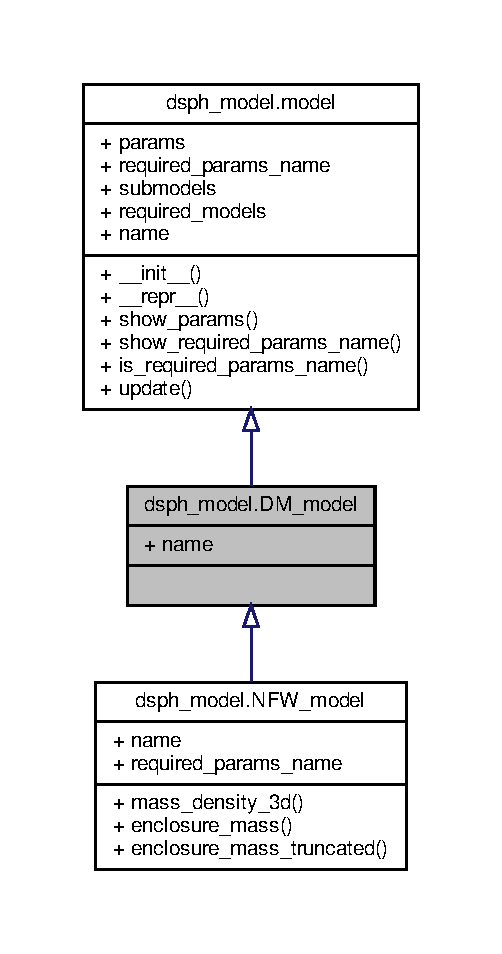
\includegraphics[width=241pt]{db/da8/classdsph__model_1_1DM__model__inherit__graph}
\end{center}
\end{figure}


Collaboration diagram for dsph\+\_\+model.\+D\+M\+\_\+model\+:\nopagebreak
\begin{figure}[H]
\begin{center}
\leavevmode
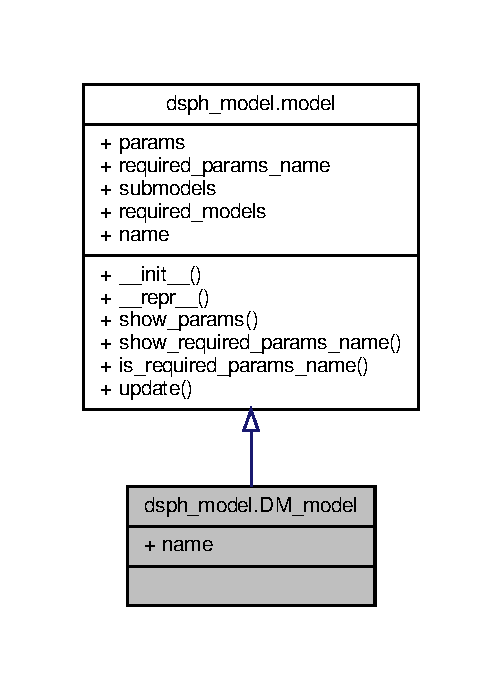
\includegraphics[width=241pt]{df/d4f/classdsph__model_1_1DM__model__coll__graph}
\end{center}
\end{figure}
\subsection*{Static Public Attributes}
\begin{DoxyCompactItemize}
\item 
string \hyperlink{classdsph__model_1_1DM__model_adb4289b632a2ad76991047f359e9d649}{name} = \char`\"{}DM \hyperlink{classdsph__model_1_1model}{model}\char`\"{}
\end{DoxyCompactItemize}
\subsection*{Additional Inherited Members}


\subsection{Detailed Description}


Definition at line 227 of file dsph\+\_\+model.\+py.



\subsection{Member Data Documentation}
\mbox{\Hypertarget{classdsph__model_1_1DM__model_adb4289b632a2ad76991047f359e9d649}\label{classdsph__model_1_1DM__model_adb4289b632a2ad76991047f359e9d649}} 
\index{dsph\+\_\+model\+::\+D\+M\+\_\+model@{dsph\+\_\+model\+::\+D\+M\+\_\+model}!name@{name}}
\index{name@{name}!dsph\+\_\+model\+::\+D\+M\+\_\+model@{dsph\+\_\+model\+::\+D\+M\+\_\+model}}
\subsubsection{\texorpdfstring{name}{name}}
{\footnotesize\ttfamily string dsph\+\_\+model.\+D\+M\+\_\+model.\+name = \char`\"{}DM \hyperlink{classdsph__model_1_1model}{model}\char`\"{}\hspace{0.3cm}{\ttfamily [static]}}



Definition at line 228 of file dsph\+\_\+model.\+py.



The documentation for this class was generated from the following file\+:\begin{DoxyCompactItemize}
\item 
memfg/\hyperlink{dsph__model_8py}{dsph\+\_\+model.\+py}\end{DoxyCompactItemize}

\hypertarget{classdsph__model_1_1dSph__model}{}\section{dsph\+\_\+model.\+d\+Sph\+\_\+model Class Reference}
\label{classdsph__model_1_1dSph__model}\index{dsph\+\_\+model.\+d\+Sph\+\_\+model@{dsph\+\_\+model.\+d\+Sph\+\_\+model}}


Inheritance diagram for dsph\+\_\+model.\+d\+Sph\+\_\+model\+:\nopagebreak
\begin{figure}[H]
\begin{center}
\leavevmode
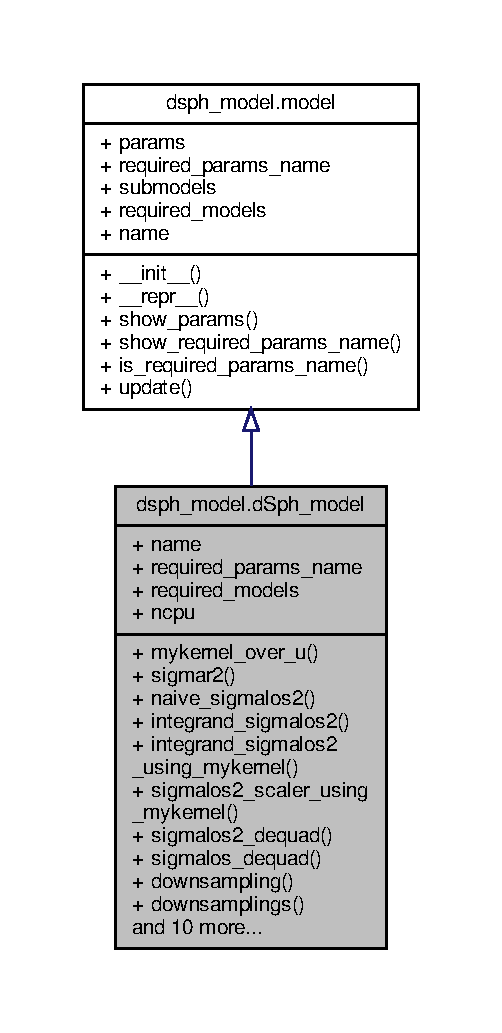
\includegraphics[width=241pt]{d5/d96/classdsph__model_1_1dSph__model__inherit__graph}
\end{center}
\end{figure}


Collaboration diagram for dsph\+\_\+model.\+d\+Sph\+\_\+model\+:\nopagebreak
\begin{figure}[H]
\begin{center}
\leavevmode
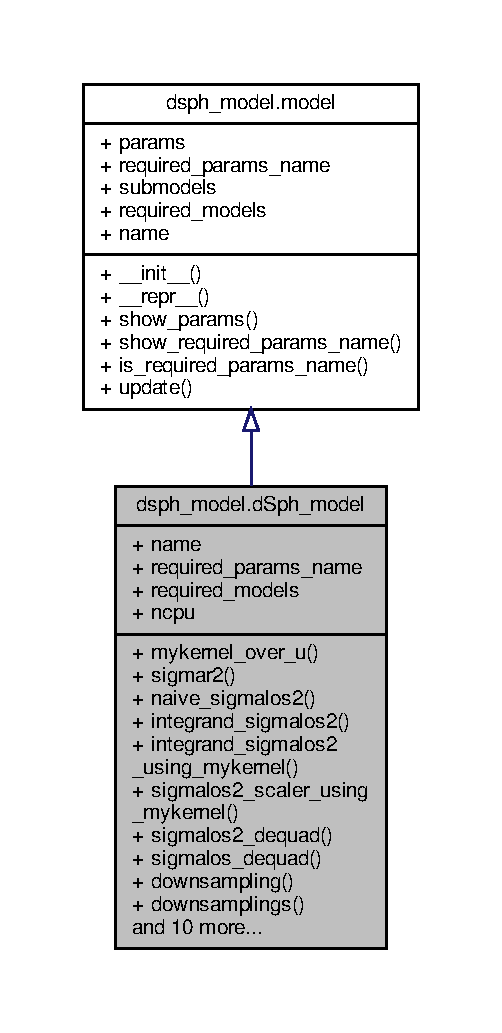
\includegraphics[width=241pt]{d6/d29/classdsph__model_1_1dSph__model__coll__graph}
\end{center}
\end{figure}
\subsection*{Public Member Functions}
\begin{DoxyCompactItemize}
\item 
def \hyperlink{classdsph__model_1_1dSph__model_a5e0091742da19919dc6c085a806ad6e0}{mykernel\+\_\+over\+\_\+u} (self, u, out=\char`\"{}linear\char`\"{})
\item 
def \hyperlink{classdsph__model_1_1dSph__model_a1c6185c02a3f58951b7ed9b75a348f49}{sigmar2} (self, r\+\_\+pc)
\item 
def \hyperlink{classdsph__model_1_1dSph__model_a9db5b642eb5007933136db35b3acf84a}{naive\+\_\+sigmalos2} (self, R\+\_\+pc)
\item 
def \hyperlink{classdsph__model_1_1dSph__model_a97bf665bdc2ff464da2c685f6f182088}{integrand\+\_\+sigmalos2} (self, c, arg\+\_\+\+R\+\_\+pc)
\item 
def \hyperlink{classdsph__model_1_1dSph__model_a5df6fa479eb9092d850da8779073eed5}{integrand\+\_\+sigmalos2\+\_\+using\+\_\+mykernel} (self, u, arg\+\_\+\+R\+\_\+pc)
\item 
def \hyperlink{classdsph__model_1_1dSph__model_a14692f81c0bffc790d5daf7f4e6464c1}{sigmalos2\+\_\+scaler\+\_\+using\+\_\+mykernel} (self, R\+\_\+pc)
\item 
def \hyperlink{classdsph__model_1_1dSph__model_a87273cf6ad641b1d12f9b236821807c6}{sigmalos2\+\_\+dequad} (self, R\+\_\+pc, dtype=np.\+float64)
\item 
def \hyperlink{classdsph__model_1_1dSph__model_a5b73e854e8ac1b1c6a467498cd181e7a}{sigmalos\+\_\+dequad} (self, R\+\_\+pc, show\+\_\+fig=False, dtype=np.\+float64, ignore\+\_\+nan=False)
\item 
def \hyperlink{classdsph__model_1_1dSph__model_a4d9e1c397b4ae379c680bc7453845781}{downsampling} (self, array, downsampling\+\_\+rate=0.\+5)
\item 
def \hyperlink{classdsph__model_1_1dSph__model_aa362ce682d90de77e755374efa153cf7}{downsamplings} (self, array, downsampling\+\_\+rate=0.\+5, iteration=1)
\item 
def \hyperlink{classdsph__model_1_1dSph__model_a0046cd7677792835d8cfafe83dbe276c}{sigmalos\+\_\+dequad\+\_\+interp1d\+\_\+downsampled} (self, R\+\_\+pc, downsampling\+\_\+rate=0.\+6, iteration=5, kind=\char`\"{}cubic\char`\"{}, offset=5, sep\+\_\+offset=1, points=\mbox{[}25., show\+\_\+fig=False, dtype=np.\+float64, ignore\+\_\+nan=True)
\item 
def \hyperlink{classdsph__model_1_1dSph__model_a05b988f7553121226a4d08369c44b4fa}{sigmalos2\+\_\+scaler} (self, R\+\_\+pc, using\+\_\+mykernel=False)
\item 
def \hyperlink{classdsph__model_1_1dSph__model_a5170edb309402dc101ea76871645e65f}{sigmalos2\+\_\+vector} (self, Rs\+\_\+pc)
\item 
def \hyperlink{classdsph__model_1_1dSph__model_a00cd796cf178fe8b3435e941976e8f27}{sigmalos2\+\_\+vector\+\_\+using\+\_\+mykernel} (self, Rs\+\_\+pc)
\item 
def \hyperlink{classdsph__model_1_1dSph__model_a0f0607e3d81520eb0c4c8b79dd871f0e}{sigmalos2\+\_\+multi\+\_\+using\+\_\+mykernel} (self, R\+\_\+pc)
\item 
def \hyperlink{classdsph__model_1_1dSph__model_a7b94850b439fe4afc431cfffa185d415}{sigmalos2} (self, R\+\_\+pc)
\item 
def \hyperlink{classdsph__model_1_1dSph__model_a4e062f0ac546057c1109fd47ec39ed90}{sigmalos2\+\_\+using\+\_\+mykernel} (self, R\+\_\+pc)
\item 
def \hyperlink{classdsph__model_1_1dSph__model_ad105b90e1827d25804eb3d7a3ba96f28}{sigmalos\+\_\+interp1d} (self, R\+\_\+pc, dR=1, d\+Rtrunc=10, step\+\_\+around\+\_\+\+Rtrunc=10, step\+\_\+outer=8, step\+\_\+center=4, kind=\char`\"{}cubic\char`\"{})
\item 
def \hyperlink{classdsph__model_1_1dSph__model_a239ec859750c30fe31b6c19e94cd2e33}{sigmalos\+\_\+interp1d\+\_\+dequad} (self, R\+\_\+pc, dR=1, d\+Rtrunc=10, step\+\_\+around\+\_\+\+Rtrunc=10, step\+\_\+outer=20, step\+\_\+center=4, kind=\char`\"{}cubic\char`\"{})
\item 
def \hyperlink{classdsph__model_1_1dSph__model_a855543fee6bd37d3b2e185c2b9dee49e}{sigmalos2\+\_\+interp1d} (self, R\+\_\+pc, step\+\_\+center=10, dR=1, d\+Rtrunc=10, step\+\_\+around\+\_\+\+Rtrunc=10, step\+\_\+before\+\_\+\+Rtrunc=8, step\+\_\+outer=8, step\+\_\+inner=16, kind=\char`\"{}cubic\char`\"{})
\end{DoxyCompactItemize}
\subsection*{Static Public Attributes}
\begin{DoxyCompactItemize}
\item 
string \hyperlink{classdsph__model_1_1dSph__model_a44e4805fa7304536056b19bd361c3d37}{name} = \textquotesingle{}\hyperlink{classdsph__model_1_1dSph__model}{d\+Sph\+\_\+model}\textquotesingle{}
\item 
list \hyperlink{classdsph__model_1_1dSph__model_a74f031f3929b9123b00121c1b02b8b71}{required\+\_\+params\+\_\+name} = \mbox{[}\textquotesingle{}anib\textquotesingle{}\mbox{]}
\item 
list \hyperlink{classdsph__model_1_1dSph__model_a7795b8e9d3d0dbf3cd5a4d618c30a6c0}{required\+\_\+models} = \mbox{[}\hyperlink{classdsph__model_1_1stellar__model}{stellar\+\_\+model},\hyperlink{classdsph__model_1_1DM__model}{D\+M\+\_\+model}\mbox{]}
\item 
\hyperlink{classdsph__model_1_1dSph__model_ab09f579bff6269075f5956a1c0a88bdc}{ncpu} = multi.\+cpu\+\_\+count()
\end{DoxyCompactItemize}
\subsection*{Additional Inherited Members}


\subsection{Detailed Description}


Definition at line 271 of file dsph\+\_\+model.\+py.



\subsection{Member Function Documentation}
\mbox{\Hypertarget{classdsph__model_1_1dSph__model_a4d9e1c397b4ae379c680bc7453845781}\label{classdsph__model_1_1dSph__model_a4d9e1c397b4ae379c680bc7453845781}} 
\index{dsph\+\_\+model\+::d\+Sph\+\_\+model@{dsph\+\_\+model\+::d\+Sph\+\_\+model}!downsampling@{downsampling}}
\index{downsampling@{downsampling}!dsph\+\_\+model\+::d\+Sph\+\_\+model@{dsph\+\_\+model\+::d\+Sph\+\_\+model}}
\subsubsection{\texorpdfstring{downsampling()}{downsampling()}}
{\footnotesize\ttfamily def dsph\+\_\+model.\+d\+Sph\+\_\+model.\+downsampling (\begin{DoxyParamCaption}\item[{}]{self,  }\item[{}]{array,  }\item[{}]{downsampling\+\_\+rate = {\ttfamily 0.5} }\end{DoxyParamCaption})}

\begin{DoxyVerb}downsampling too dense ones.
\end{DoxyVerb}
 

Definition at line 379 of file dsph\+\_\+model.\+py.


\begin{DoxyCode}
379     \textcolor{keyword}{def }downsampling(self,array,downsampling\_rate=0.5):
380         \textcolor{stringliteral}{'''}
381 \textcolor{stringliteral}{        downsampling too dense ones.}
382 \textcolor{stringliteral}{        '''}
383         ordered\_array = sort(array)
384         arg\_ordered\_array = argsort(array)
385         diff = ordered\_array[1:] - ordered\_array[:-1]
386         arg\_arg\_ordered\_array = argsort(diff)[int(downsampling\_rate*len(array)):] \textcolor{comment}{# ordering by diff and
       extract not too dense ones}
387         \textcolor{comment}{#display(pd.DataFrame(\{"arg\_ordered\_array":arg\_ordered\_array,"array":array\}))}
388         \textcolor{comment}{#display(pd.DataFrame(\{"arg\_arg\_ordered\_array":arg\_arg\_ordered\_array\}))}
389         \textcolor{keywordflow}{return} array[arg\_ordered\_array[arg\_arg\_ordered\_array]]
390     
\end{DoxyCode}
Here is the caller graph for this function\+:\nopagebreak
\begin{figure}[H]
\begin{center}
\leavevmode
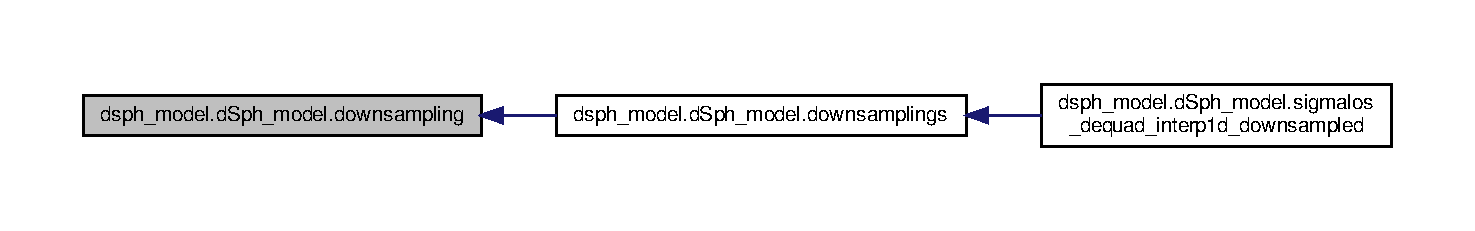
\includegraphics[width=350pt]{d0/d25/classdsph__model_1_1dSph__model_a4d9e1c397b4ae379c680bc7453845781_icgraph}
\end{center}
\end{figure}
\mbox{\Hypertarget{classdsph__model_1_1dSph__model_aa362ce682d90de77e755374efa153cf7}\label{classdsph__model_1_1dSph__model_aa362ce682d90de77e755374efa153cf7}} 
\index{dsph\+\_\+model\+::d\+Sph\+\_\+model@{dsph\+\_\+model\+::d\+Sph\+\_\+model}!downsamplings@{downsamplings}}
\index{downsamplings@{downsamplings}!dsph\+\_\+model\+::d\+Sph\+\_\+model@{dsph\+\_\+model\+::d\+Sph\+\_\+model}}
\subsubsection{\texorpdfstring{downsamplings()}{downsamplings()}}
{\footnotesize\ttfamily def dsph\+\_\+model.\+d\+Sph\+\_\+model.\+downsamplings (\begin{DoxyParamCaption}\item[{}]{self,  }\item[{}]{array,  }\item[{}]{downsampling\+\_\+rate = {\ttfamily 0.5},  }\item[{}]{iteration = {\ttfamily 1} }\end{DoxyParamCaption})}



Definition at line 391 of file dsph\+\_\+model.\+py.


\begin{DoxyCode}
391     \textcolor{keyword}{def }downsamplings(self,array,downsampling\_rate=0.5,iteration=1):
392         ret = array
393         func = self.downsampling
394         \textcolor{comment}{#print("print array")}
395         \textcolor{comment}{#display(ret)}
396         \textcolor{keywordflow}{for} i \textcolor{keywordflow}{in} range(iteration):
397             \textcolor{comment}{#print("print return i:\{\}".format(i))}
398             ret = func(ret,downsampling\_rate)
399             \textcolor{comment}{#display(ret)}
400         \textcolor{keywordflow}{return} ret
401     
\end{DoxyCode}
Here is the call graph for this function\+:\nopagebreak
\begin{figure}[H]
\begin{center}
\leavevmode
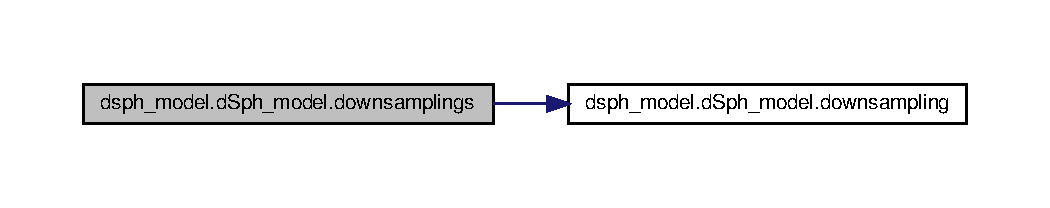
\includegraphics[width=350pt]{d0/d25/classdsph__model_1_1dSph__model_aa362ce682d90de77e755374efa153cf7_cgraph}
\end{center}
\end{figure}
Here is the caller graph for this function\+:\nopagebreak
\begin{figure}[H]
\begin{center}
\leavevmode
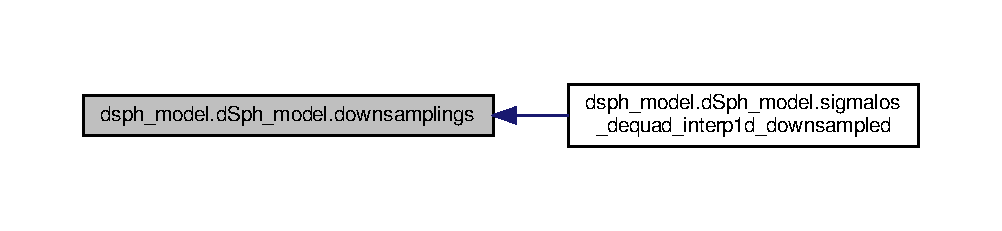
\includegraphics[width=350pt]{d0/d25/classdsph__model_1_1dSph__model_aa362ce682d90de77e755374efa153cf7_icgraph}
\end{center}
\end{figure}
\mbox{\Hypertarget{classdsph__model_1_1dSph__model_a97bf665bdc2ff464da2c685f6f182088}\label{classdsph__model_1_1dSph__model_a97bf665bdc2ff464da2c685f6f182088}} 
\index{dsph\+\_\+model\+::d\+Sph\+\_\+model@{dsph\+\_\+model\+::d\+Sph\+\_\+model}!integrand\+\_\+sigmalos2@{integrand\+\_\+sigmalos2}}
\index{integrand\+\_\+sigmalos2@{integrand\+\_\+sigmalos2}!dsph\+\_\+model\+::d\+Sph\+\_\+model@{dsph\+\_\+model\+::d\+Sph\+\_\+model}}
\subsubsection{\texorpdfstring{integrand\+\_\+sigmalos2()}{integrand\_sigmalos2()}}
{\footnotesize\ttfamily def dsph\+\_\+model.\+d\+Sph\+\_\+model.\+integrand\+\_\+sigmalos2 (\begin{DoxyParamCaption}\item[{}]{self,  }\item[{}]{c,  }\item[{}]{arg\+\_\+\+R\+\_\+pc }\end{DoxyParamCaption})}

\begin{DoxyVerb}integrand of sigmalos2 at R = R_pc.
c is a variable of integration, related to u (=r/R) as u = 1/c.
domain: 0 < c < 1, OR 1 < u < oo.
The variable c has the mean of cos(\theta), where \theta is the angle of the popsition of integration
on the LINE-of-sight. (integration on los)
\end{DoxyVerb}
 

Definition at line 315 of file dsph\+\_\+model.\+py.


\begin{DoxyCode}
315     \textcolor{keyword}{def }integrand\_sigmalos2(self,c,arg\_R\_pc):
316         \textcolor{stringliteral}{'''}
317 \textcolor{stringliteral}{        integrand of sigmalos2 at R = R\_pc.}
318 \textcolor{stringliteral}{        c is a variable of integration, related to u (=r/R) as u = 1/c.}
319 \textcolor{stringliteral}{        domain: 0 < c < 1, OR 1 < u < oo.}
320 \textcolor{stringliteral}{        The variable c has the mean of cos(\(\backslash\)theta), where \(\backslash\)theta is the angle of the popsition of
       integration}
321 \textcolor{stringliteral}{        on the LINE-of-sight. (integration on los)}
322 \textcolor{stringliteral}{        '''}
323         params\_dSph,params\_stellar,params\_DM = self.params,self.submodels[\textcolor{stringliteral}{"stellar\_model"}].params,self.
      submodels[\textcolor{stringliteral}{"DM\_model"}].params
324         anib = params\_dSph.anib
325         \textcolor{comment}{#print(params\_dSph,params\_stellar,params\_DM)}
326         rhos\_Msunpc3,rs\_pc,a,b,g = [params\_DM[key] \textcolor{keywordflow}{for} key \textcolor{keywordflow}{in} (\textcolor{stringliteral}{'rhos\_Msunpc3'},\textcolor{stringliteral}{'rs\_pc'},\textcolor{stringliteral}{'a'},\textcolor{stringliteral}{'b'},\textcolor{stringliteral}{'g'})]
327         re\_pc = params\_stellar.re\_pc
328         u2 = 1./c/c
329         
332         \textcolor{keywordflow}{return} sqrt(u2-1)*((1.5-anib)*u2*hyp2f1(1.0,1.5-anib,1.5,1-u2)-0.5) * self.submodels[\textcolor{stringliteral}{"stellar\_model
      "}].density\_3d(arg\_R\_pc/c)*GMsun\_m3s2*self.submodels[\textcolor{stringliteral}{"DM\_model"}].enclosure\_mass(arg\_R\_pc/c)/parsec \textcolor{comment}{# NOTE:
       without u^-2 !! 1/parsec because we divide it by Sigmaast [pc^-2] so convert one of [m] -> [pc]  }
333     
\end{DoxyCode}
Here is the caller graph for this function\+:\nopagebreak
\begin{figure}[H]
\begin{center}
\leavevmode
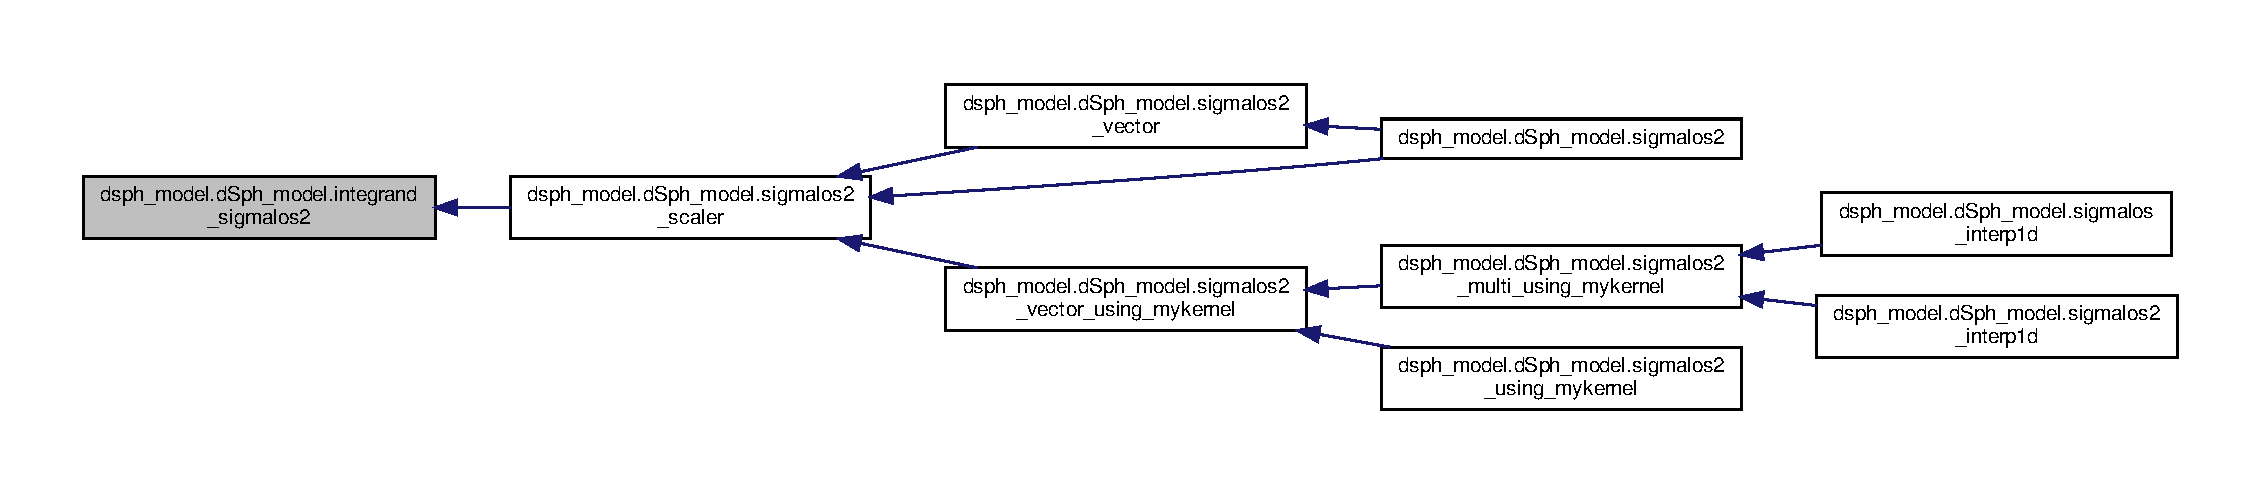
\includegraphics[width=350pt]{d0/d25/classdsph__model_1_1dSph__model_a97bf665bdc2ff464da2c685f6f182088_icgraph}
\end{center}
\end{figure}
\mbox{\Hypertarget{classdsph__model_1_1dSph__model_a5df6fa479eb9092d850da8779073eed5}\label{classdsph__model_1_1dSph__model_a5df6fa479eb9092d850da8779073eed5}} 
\index{dsph\+\_\+model\+::d\+Sph\+\_\+model@{dsph\+\_\+model\+::d\+Sph\+\_\+model}!integrand\+\_\+sigmalos2\+\_\+using\+\_\+mykernel@{integrand\+\_\+sigmalos2\+\_\+using\+\_\+mykernel}}
\index{integrand\+\_\+sigmalos2\+\_\+using\+\_\+mykernel@{integrand\+\_\+sigmalos2\+\_\+using\+\_\+mykernel}!dsph\+\_\+model\+::d\+Sph\+\_\+model@{dsph\+\_\+model\+::d\+Sph\+\_\+model}}
\subsubsection{\texorpdfstring{integrand\+\_\+sigmalos2\+\_\+using\+\_\+mykernel()}{integrand\_sigmalos2\_using\_mykernel()}}
{\footnotesize\ttfamily def dsph\+\_\+model.\+d\+Sph\+\_\+model.\+integrand\+\_\+sigmalos2\+\_\+using\+\_\+mykernel (\begin{DoxyParamCaption}\item[{}]{self,  }\item[{}]{u,  }\item[{}]{arg\+\_\+\+R\+\_\+pc }\end{DoxyParamCaption})}

\begin{DoxyVerb}integrand of sigmalos2 at R = R_pc.
u is a variable of integration, u=r/R.
Domain: 1 < u < oo.
\end{DoxyVerb}
 

Definition at line 334 of file dsph\+\_\+model.\+py.


\begin{DoxyCode}
334     \textcolor{keyword}{def }integrand\_sigmalos2\_using\_mykernel(self,u,arg\_R\_pc):
335         \textcolor{stringliteral}{'''}
336 \textcolor{stringliteral}{        integrand of sigmalos2 at R = R\_pc.}
337 \textcolor{stringliteral}{        u is a variable of integration, u=r/R.}
338 \textcolor{stringliteral}{        Domain: 1 < u < oo.}
339 \textcolor{stringliteral}{        '''}
340         stellar\_model,DM\_model = self.submodels[\textcolor{stringliteral}{"stellar\_model"}],self.submodels[\textcolor{stringliteral}{"DM\_model"}]
341         u2,r = u**2,arg\_R\_pc*u
342         \textcolor{comment}{# Note that parsec = parsec/m.}
343         \textcolor{comment}{# If you convert m -> pc,      ... var[m] * [1 pc/ parsec m] = var/parsec[pc].}
344         \textcolor{comment}{#                pc^1 -> m^pc, ... var[pc^1] * parsec(=[pc/m]) = var[m^-1]}
345         \textcolor{comment}{# Here var[m^3 pc^-1 s^-2] /parsec[m/pc] * 1e-6[km^2/m^2] = var[km^2/s^2]}
346         \textcolor{keywordflow}{return} 2 * self.mykernel\_over\_u(u) *  stellar\_model.density\_3d(r)/stellar\_model.density\_2d(arg\_R\_pc
      )*GMsun\_m3s2 * DM\_model.enclosure\_mass(r) / parsec * 1e-6
347 
\end{DoxyCode}
Here is the call graph for this function\+:\nopagebreak
\begin{figure}[H]
\begin{center}
\leavevmode
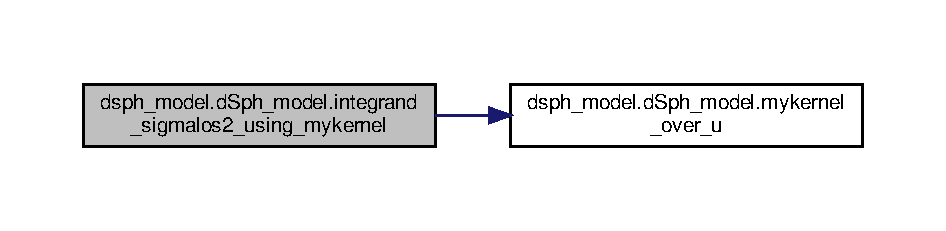
\includegraphics[width=350pt]{d0/d25/classdsph__model_1_1dSph__model_a5df6fa479eb9092d850da8779073eed5_cgraph}
\end{center}
\end{figure}
Here is the caller graph for this function\+:\nopagebreak
\begin{figure}[H]
\begin{center}
\leavevmode
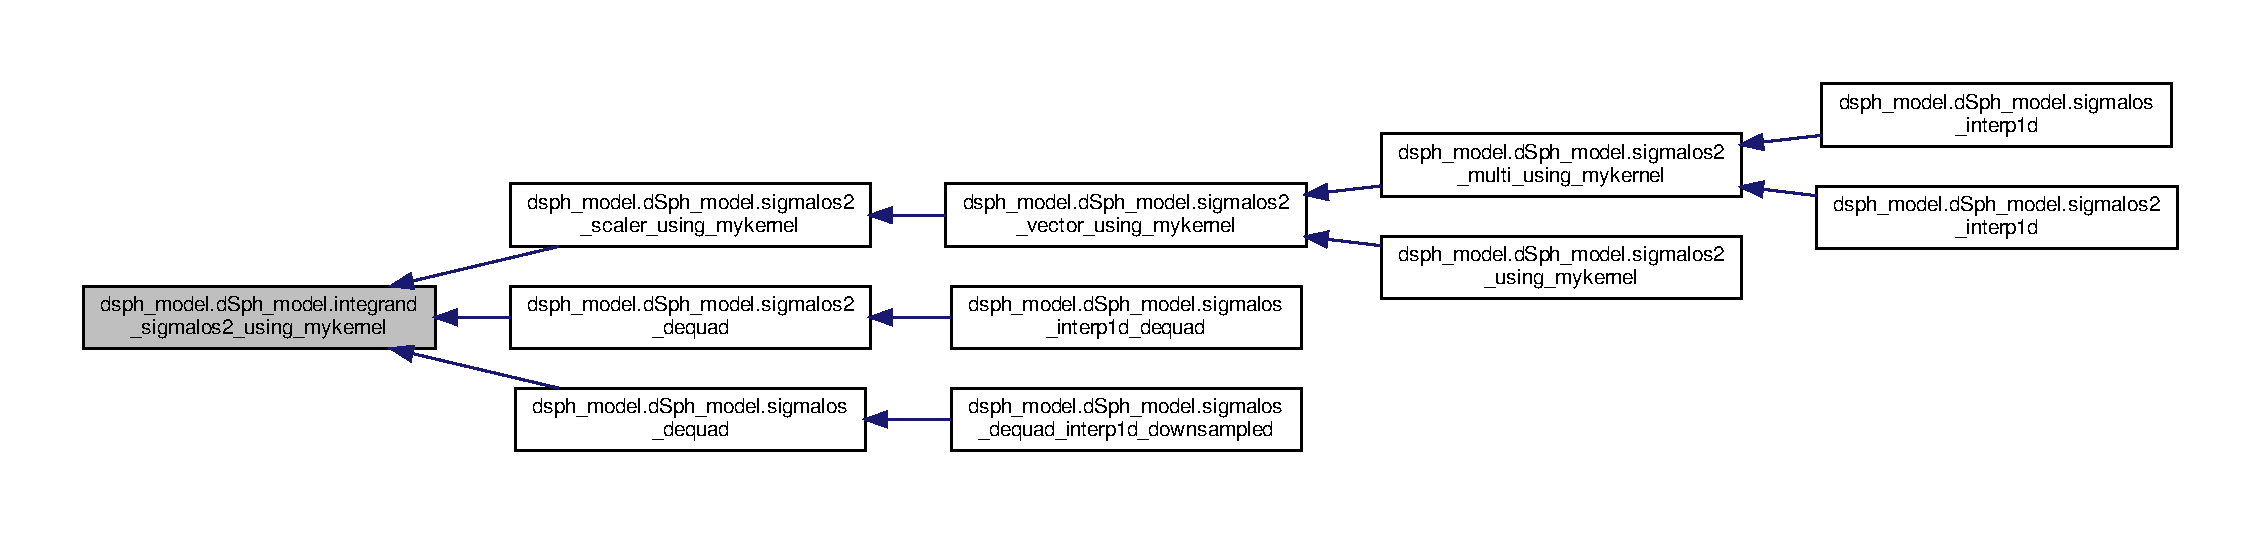
\includegraphics[width=350pt]{d0/d25/classdsph__model_1_1dSph__model_a5df6fa479eb9092d850da8779073eed5_icgraph}
\end{center}
\end{figure}
\mbox{\Hypertarget{classdsph__model_1_1dSph__model_a5e0091742da19919dc6c085a806ad6e0}\label{classdsph__model_1_1dSph__model_a5e0091742da19919dc6c085a806ad6e0}} 
\index{dsph\+\_\+model\+::d\+Sph\+\_\+model@{dsph\+\_\+model\+::d\+Sph\+\_\+model}!mykernel\+\_\+over\+\_\+u@{mykernel\+\_\+over\+\_\+u}}
\index{mykernel\+\_\+over\+\_\+u@{mykernel\+\_\+over\+\_\+u}!dsph\+\_\+model\+::d\+Sph\+\_\+model@{dsph\+\_\+model\+::d\+Sph\+\_\+model}}
\subsubsection{\texorpdfstring{mykernel\+\_\+over\+\_\+u()}{mykernel\_over\_u()}}
{\footnotesize\ttfamily def dsph\+\_\+model.\+d\+Sph\+\_\+model.\+mykernel\+\_\+over\+\_\+u (\begin{DoxyParamCaption}\item[{}]{self,  }\item[{}]{u,  }\item[{}]{out = {\ttfamily \char`\"{}linear\char`\"{}} }\end{DoxyParamCaption})}

\begin{DoxyVerb}My kernel over u. Using 2F1.Using this kernel over u K(u)/u, sigmalos2 is given by
    sigmalos2(R) = 2 * \int_1^oo du \Sigma_\ast(uR)/\nu_\ast(R) * GM(uR) * K(u)/u.
    
Descriptions:
    args: u = r_integrated/R, 1<u<oo
\end{DoxyVerb}
 

Definition at line 284 of file dsph\+\_\+model.\+py.


\begin{DoxyCode}
284     \textcolor{keyword}{def }mykernel\_over\_u(self,u,out="linear"):
285         \textcolor{stringliteral}{'''}
286 \textcolor{stringliteral}{        My kernel over u. Using 2F1.Using this kernel over u K(u)/u, sigmalos2 is given by}
287 \textcolor{stringliteral}{            sigmalos2(R) = 2 * \(\backslash\)int\_1^oo du \(\backslash\)Sigma\_\(\backslash\)ast(uR)/\(\backslash\)nu\_\(\backslash\)ast(R) * GM(uR) * K(u)/u.}
288 \textcolor{stringliteral}{            }
289 \textcolor{stringliteral}{        Descriptions:}
290 \textcolor{stringliteral}{            args: u = r\_integrated/R, 1<u<oo}
291 \textcolor{stringliteral}{        '''}
292         anib = self.params.anib
293         u2 = u**2
294         \textcolor{keywordflow}{if} out==\textcolor{stringliteral}{"linear"}:
295             \textcolor{keywordflow}{return} 1/u * sqrt(1-1/u2)*((1.5-anib)*u2*hyp2f1(1.0,1.5-anib,1.5,1-u2)-0.5)
296         \textcolor{keywordflow}{elif} out==\textcolor{stringliteral}{"log"}:
297             \textcolor{keywordflow}{return} -log(u) + log(1-1/u2)/2 + log((1.5-anib)*u2*hyp2f1(1.0,1.5-anib,1.5,1-u2)-0.5)
298 
\end{DoxyCode}
Here is the caller graph for this function\+:\nopagebreak
\begin{figure}[H]
\begin{center}
\leavevmode
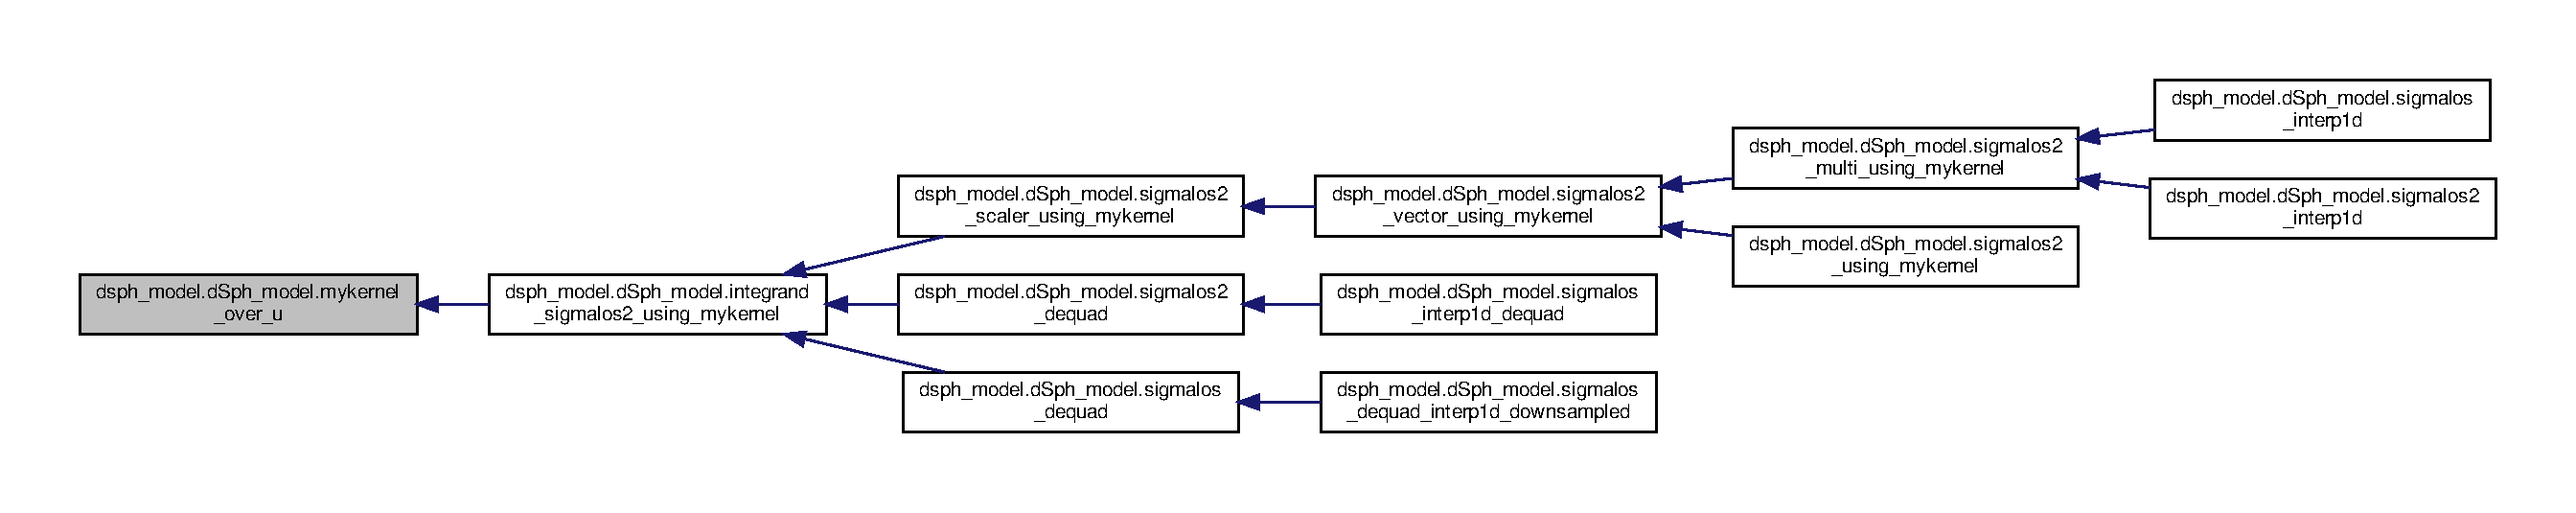
\includegraphics[width=350pt]{d0/d25/classdsph__model_1_1dSph__model_a5e0091742da19919dc6c085a806ad6e0_icgraph}
\end{center}
\end{figure}
\mbox{\Hypertarget{classdsph__model_1_1dSph__model_a9db5b642eb5007933136db35b3acf84a}\label{classdsph__model_1_1dSph__model_a9db5b642eb5007933136db35b3acf84a}} 
\index{dsph\+\_\+model\+::d\+Sph\+\_\+model@{dsph\+\_\+model\+::d\+Sph\+\_\+model}!naive\+\_\+sigmalos2@{naive\+\_\+sigmalos2}}
\index{naive\+\_\+sigmalos2@{naive\+\_\+sigmalos2}!dsph\+\_\+model\+::d\+Sph\+\_\+model@{dsph\+\_\+model\+::d\+Sph\+\_\+model}}
\subsubsection{\texorpdfstring{naive\+\_\+sigmalos2()}{naive\_sigmalos2()}}
{\footnotesize\ttfamily def dsph\+\_\+model.\+d\+Sph\+\_\+model.\+naive\+\_\+sigmalos2 (\begin{DoxyParamCaption}\item[{}]{self,  }\item[{}]{R\+\_\+pc }\end{DoxyParamCaption})}



Definition at line 306 of file dsph\+\_\+model.\+py.


\begin{DoxyCode}
306     \textcolor{keyword}{def }naive\_sigmalos2(self,R\_pc):
307         RELERROR\_INTEG = 1e-6
308         anib = self.params.anib
309         integrand = \textcolor{keyword}{lambda} r: (1-anib*(R\_pc/r)**2)*self.submodels[\textcolor{stringliteral}{"stellar\_model"}].density\_3d(r)*self.
      sigmar2(r)/np.sqrt(1-(R\_pc/r)**2)
310         rs\_interp = np.logspace(-2,6,51)
311         integrand\_interp = interp1d(rs\_interp,[integrand(r) \textcolor{keywordflow}{for} r \textcolor{keywordflow}{in} rs\_interp],kind=\textcolor{stringliteral}{"quadratic"}) 
312         integ, abserr = integrate.quad(integrand\_interp,R\_pc,np.inf)
313         \textcolor{keywordflow}{return} 2*integ/self.submodels[\textcolor{stringliteral}{"stellar\_model"}].density\_2d(R\_pc)
314     
\end{DoxyCode}
Here is the call graph for this function\+:\nopagebreak
\begin{figure}[H]
\begin{center}
\leavevmode
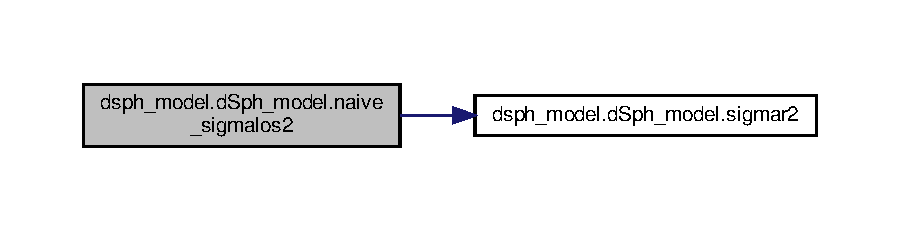
\includegraphics[width=350pt]{d0/d25/classdsph__model_1_1dSph__model_a9db5b642eb5007933136db35b3acf84a_cgraph}
\end{center}
\end{figure}
\mbox{\Hypertarget{classdsph__model_1_1dSph__model_a7b94850b439fe4afc431cfffa185d415}\label{classdsph__model_1_1dSph__model_a7b94850b439fe4afc431cfffa185d415}} 
\index{dsph\+\_\+model\+::d\+Sph\+\_\+model@{dsph\+\_\+model\+::d\+Sph\+\_\+model}!sigmalos2@{sigmalos2}}
\index{sigmalos2@{sigmalos2}!dsph\+\_\+model\+::d\+Sph\+\_\+model@{dsph\+\_\+model\+::d\+Sph\+\_\+model}}
\subsubsection{\texorpdfstring{sigmalos2()}{sigmalos2()}}
{\footnotesize\ttfamily def dsph\+\_\+model.\+d\+Sph\+\_\+model.\+sigmalos2 (\begin{DoxyParamCaption}\item[{}]{self,  }\item[{}]{R\+\_\+pc }\end{DoxyParamCaption})}



Definition at line 439 of file dsph\+\_\+model.\+py.


\begin{DoxyCode}
439     \textcolor{keyword}{def }sigmalos2(self,R\_pc):
440         \textcolor{keywordflow}{return} (self.sigmalos2\_scaler(R\_pc) \textcolor{keywordflow}{if} len(R\_pc)==1 \textcolor{keywordflow}{else} self.sigmalos2\_vector(R\_pc))
441     
\end{DoxyCode}
Here is the call graph for this function\+:\nopagebreak
\begin{figure}[H]
\begin{center}
\leavevmode
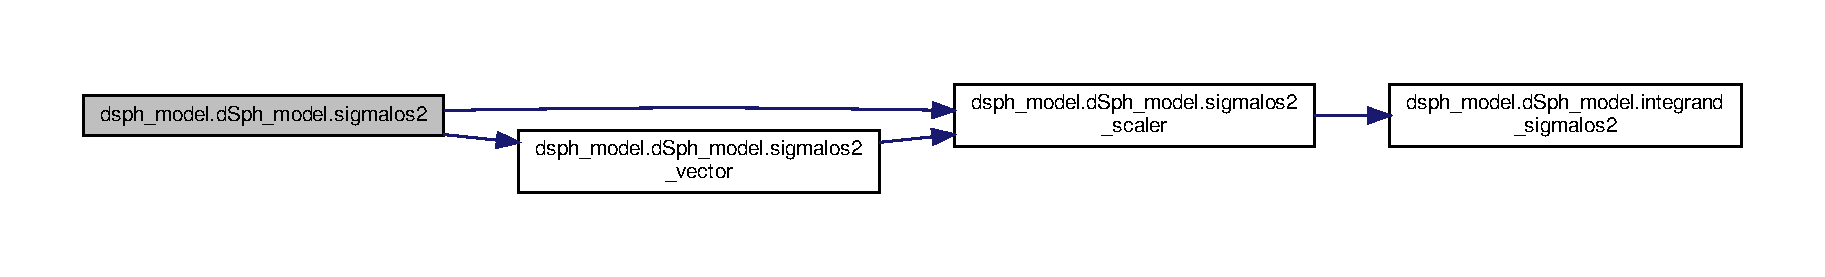
\includegraphics[width=350pt]{d0/d25/classdsph__model_1_1dSph__model_a7b94850b439fe4afc431cfffa185d415_cgraph}
\end{center}
\end{figure}
\mbox{\Hypertarget{classdsph__model_1_1dSph__model_a87273cf6ad641b1d12f9b236821807c6}\label{classdsph__model_1_1dSph__model_a87273cf6ad641b1d12f9b236821807c6}} 
\index{dsph\+\_\+model\+::d\+Sph\+\_\+model@{dsph\+\_\+model\+::d\+Sph\+\_\+model}!sigmalos2\+\_\+dequad@{sigmalos2\+\_\+dequad}}
\index{sigmalos2\+\_\+dequad@{sigmalos2\+\_\+dequad}!dsph\+\_\+model\+::d\+Sph\+\_\+model@{dsph\+\_\+model\+::d\+Sph\+\_\+model}}
\subsubsection{\texorpdfstring{sigmalos2\+\_\+dequad()}{sigmalos2\_dequad()}}
{\footnotesize\ttfamily def dsph\+\_\+model.\+d\+Sph\+\_\+model.\+sigmalos2\+\_\+dequad (\begin{DoxyParamCaption}\item[{}]{self,  }\item[{}]{R\+\_\+pc,  }\item[{}]{dtype = {\ttfamily np.float64} }\end{DoxyParamCaption})}



Definition at line 362 of file dsph\+\_\+model.\+py.


\begin{DoxyCode}
362     \textcolor{keyword}{def }sigmalos2\_dequad(self,R\_pc,dtype=np.float64):
363         \textcolor{keyword}{def }func(u):
364             u\_ = np.array(u)[np.newaxis,:]
365             R\_pc\_ = np.array(R\_pc)[:,np.newaxis]
366             \textcolor{keywordflow}{return} self.integrand\_sigmalos2\_using\_mykernel(u\_,R\_pc\_)
367         ret = \hyperlink{namespacedequad_a2654bb61f33ab8685320882396c81ae0}{dequad\_hinf}(func,1,axis=1,width=5e-3,pN=1000,mN=1000,dtype=np.dtype,show\_fig=
      show\_fig)
368         \textcolor{keywordflow}{if} np.any(isnan(ret)):
369             \textcolor{keywordflow}{raise} TypeError(\textcolor{stringliteral}{"nan! \{\}"}.format(ret))
370         \textcolor{keywordflow}{return} ret
371     
\end{DoxyCode}
Here is the call graph for this function\+:\nopagebreak
\begin{figure}[H]
\begin{center}
\leavevmode
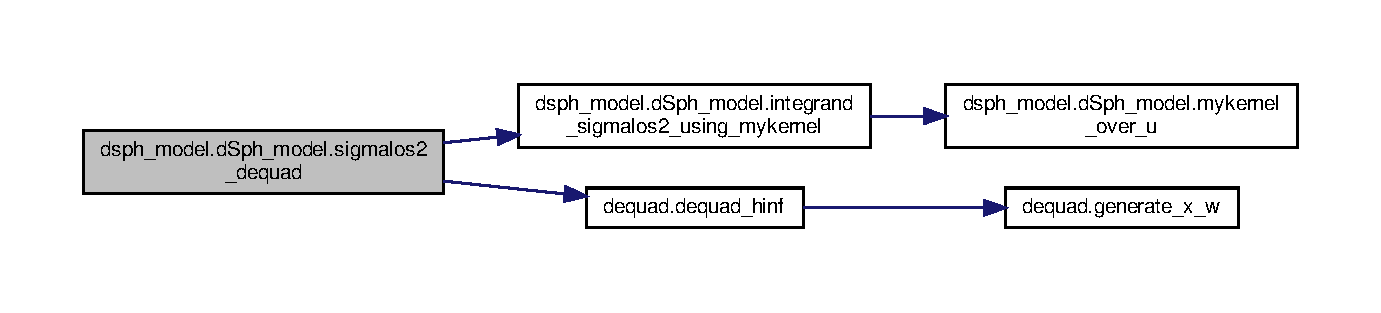
\includegraphics[width=350pt]{d0/d25/classdsph__model_1_1dSph__model_a87273cf6ad641b1d12f9b236821807c6_cgraph}
\end{center}
\end{figure}
Here is the caller graph for this function\+:\nopagebreak
\begin{figure}[H]
\begin{center}
\leavevmode
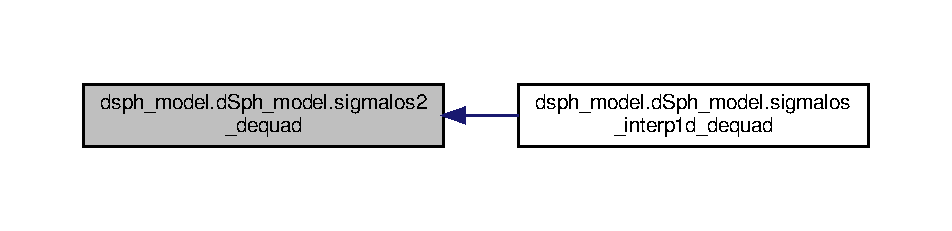
\includegraphics[width=350pt]{d0/d25/classdsph__model_1_1dSph__model_a87273cf6ad641b1d12f9b236821807c6_icgraph}
\end{center}
\end{figure}
\mbox{\Hypertarget{classdsph__model_1_1dSph__model_a855543fee6bd37d3b2e185c2b9dee49e}\label{classdsph__model_1_1dSph__model_a855543fee6bd37d3b2e185c2b9dee49e}} 
\index{dsph\+\_\+model\+::d\+Sph\+\_\+model@{dsph\+\_\+model\+::d\+Sph\+\_\+model}!sigmalos2\+\_\+interp1d@{sigmalos2\+\_\+interp1d}}
\index{sigmalos2\+\_\+interp1d@{sigmalos2\+\_\+interp1d}!dsph\+\_\+model\+::d\+Sph\+\_\+model@{dsph\+\_\+model\+::d\+Sph\+\_\+model}}
\subsubsection{\texorpdfstring{sigmalos2\+\_\+interp1d()}{sigmalos2\_interp1d()}}
{\footnotesize\ttfamily def dsph\+\_\+model.\+d\+Sph\+\_\+model.\+sigmalos2\+\_\+interp1d (\begin{DoxyParamCaption}\item[{}]{self,  }\item[{}]{R\+\_\+pc,  }\item[{}]{step\+\_\+center = {\ttfamily 10},  }\item[{}]{dR = {\ttfamily 1},  }\item[{}]{d\+Rtrunc = {\ttfamily 10},  }\item[{}]{step\+\_\+around\+\_\+\+Rtrunc = {\ttfamily 10},  }\item[{}]{step\+\_\+before\+\_\+\+Rtrunc = {\ttfamily 8},  }\item[{}]{step\+\_\+outer = {\ttfamily 8},  }\item[{}]{step\+\_\+inner = {\ttfamily 16},  }\item[{}]{kind = {\ttfamily \char`\"{}cubic\char`\"{}} }\end{DoxyParamCaption})}

\begin{DoxyVerb}inner part has large error, so more refine interp
\end{DoxyVerb}
 

Definition at line 489 of file dsph\+\_\+model.\+py.


\begin{DoxyCode}
489     \textcolor{keyword}{def }sigmalos2\_interp1d(
      self,R\_pc,step\_center=10,dR=1,dRtrunc=10,step\_around\_Rtrunc=10,step\_before\_Rtrunc=8,step\_outer=8,step\_inner=16,kind="cubic"):
490         \textcolor{stringliteral}{'''}
491 \textcolor{stringliteral}{        inner part has large error, so more refine interp}
492 \textcolor{stringliteral}{        '''}
493         re = self.submodels[\textcolor{stringliteral}{"stellar\_model"}].params.re\_pc
494         Rtrunc = self.submodels[\textcolor{stringliteral}{"DM\_model"}].params.R\_trunc\_pc
495         n = len(R\_pc)
496         R\_pc\_sorted\_ = np.sort(R\_pc)
497         R\_pc\_around\_Rtrunc = np.sort(R\_pc\_sorted\_[np.argsort(np.abs(R\_pc\_sorted\_-Rtrunc))[:
      step\_around\_Rtrunc]])
498         Rmin,Rmax = R\_pc\_sorted\_[0],R\_pc\_sorted\_[-1]
499         \textcolor{comment}{#R\_pc\_lo\_ = np.linspace(Rmin*0.5,Rmin*1.5,int((n*0.2)/step))}
500         \textcolor{comment}{#R\_pc\_lo\_ = R\_pc\_sorted\_[:int(n*0.05)]}
501         \textcolor{comment}{#R\_pc\_hi\_ = np.linspace(R\_pc\_lo\_[-1]+0.1,Rmax*1.1,int(n/step))}
502         \textcolor{comment}{#R\_pc\_ = np.hstack((R\_pc\_lo\_,R\_pc\_hi\_))}
503         R\_pc\_zero = R\_pc\_sorted\_[:step\_center]
504         R\_pc\_lo\_ = np.linspace(R\_pc\_sorted\_[step\_center],R\_pc\_sorted\_[R\_pc\_sorted\_<re][-1],step\_inner)
505         R\_pc\_hi\_ = np.linspace(re,Rmax,step\_outer)
506         R\_pc\_ = np.sort(np.unique(np.concatenate((R\_pc\_zero,R\_pc\_lo\_,R\_pc\_around\_Rtrunc,R\_pc\_hi\_),axis=\textcolor{keywordtype}{None}
      )))
507         \textcolor{comment}{#R\_pc\_ = np.linspace(Rmin,Rmax,int(n/step))}
508         sigmalos2\_ = self.sigmalos2\_multi\_using\_mykernel(R\_pc\_)
509         interpd\_func = interp1d(R\_pc\_, sigmalos2\_,kind=kind)
510         \textcolor{keywordflow}{return} interpd\_func(R\_pc) \textcolor{comment}{# here R\_pc is original, so return unsorted results}
511         
512 
\end{DoxyCode}
Here is the call graph for this function\+:\nopagebreak
\begin{figure}[H]
\begin{center}
\leavevmode
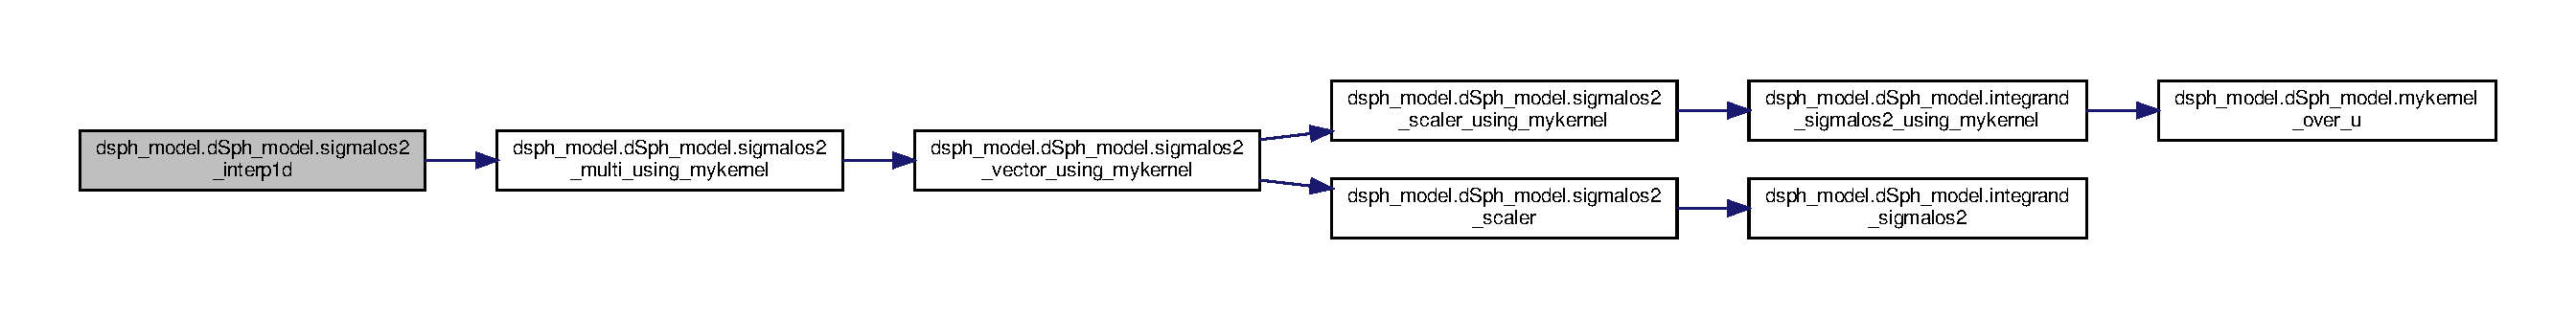
\includegraphics[width=350pt]{d0/d25/classdsph__model_1_1dSph__model_a855543fee6bd37d3b2e185c2b9dee49e_cgraph}
\end{center}
\end{figure}
\mbox{\Hypertarget{classdsph__model_1_1dSph__model_a0f0607e3d81520eb0c4c8b79dd871f0e}\label{classdsph__model_1_1dSph__model_a0f0607e3d81520eb0c4c8b79dd871f0e}} 
\index{dsph\+\_\+model\+::d\+Sph\+\_\+model@{dsph\+\_\+model\+::d\+Sph\+\_\+model}!sigmalos2\+\_\+multi\+\_\+using\+\_\+mykernel@{sigmalos2\+\_\+multi\+\_\+using\+\_\+mykernel}}
\index{sigmalos2\+\_\+multi\+\_\+using\+\_\+mykernel@{sigmalos2\+\_\+multi\+\_\+using\+\_\+mykernel}!dsph\+\_\+model\+::d\+Sph\+\_\+model@{dsph\+\_\+model\+::d\+Sph\+\_\+model}}
\subsubsection{\texorpdfstring{sigmalos2\+\_\+multi\+\_\+using\+\_\+mykernel()}{sigmalos2\_multi\_using\_mykernel()}}
{\footnotesize\ttfamily def dsph\+\_\+model.\+d\+Sph\+\_\+model.\+sigmalos2\+\_\+multi\+\_\+using\+\_\+mykernel (\begin{DoxyParamCaption}\item[{}]{self,  }\item[{}]{R\+\_\+pc }\end{DoxyParamCaption})}



Definition at line 431 of file dsph\+\_\+model.\+py.


\begin{DoxyCode}
431     \textcolor{keyword}{def }sigmalos2\_multi\_using\_mykernel(self,R\_pc):
432         p = Pool(self.ncpu)
433         R\_pc\_splited = np.array\_split(R\_pc,self.ncpu)
434         \textcolor{comment}{#args = [(Rs,anib,rhos\_Msunpc3,rs\_pc,a,b,g,re\_pc) for Rs in R\_pc\_v\_splited]}
435         ret = p.map(self.sigmalos2\_vector\_using\_mykernel,R\_pc\_splited)
436         p.close()
437         \textcolor{keywordflow}{return} np.concatenate(ret)
438 
\end{DoxyCode}
Here is the call graph for this function\+:\nopagebreak
\begin{figure}[H]
\begin{center}
\leavevmode
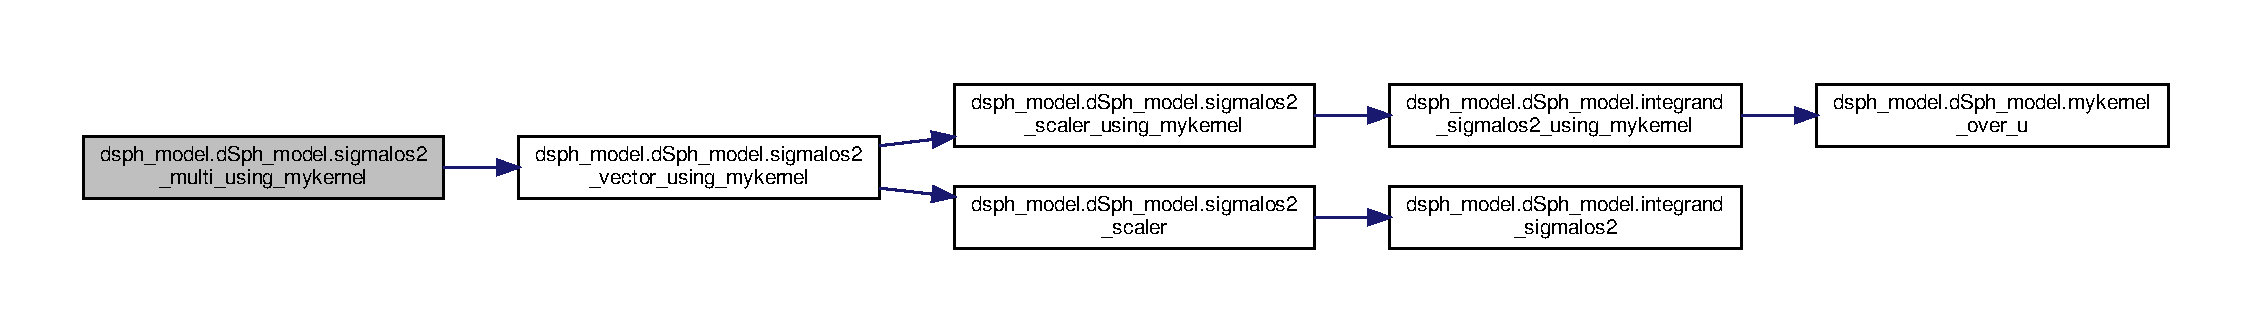
\includegraphics[width=350pt]{d0/d25/classdsph__model_1_1dSph__model_a0f0607e3d81520eb0c4c8b79dd871f0e_cgraph}
\end{center}
\end{figure}
Here is the caller graph for this function\+:\nopagebreak
\begin{figure}[H]
\begin{center}
\leavevmode
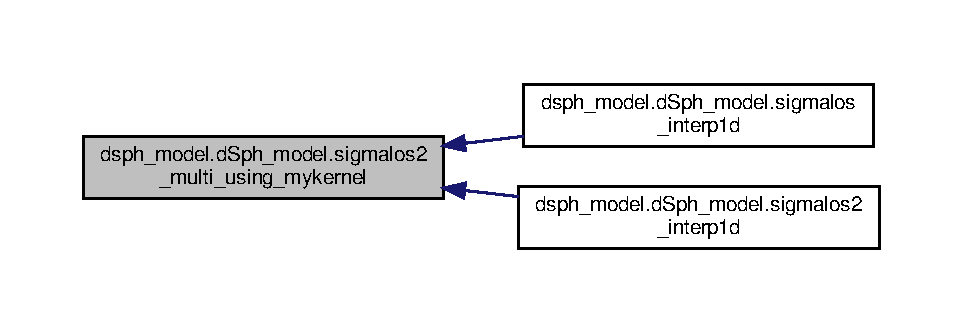
\includegraphics[width=350pt]{d0/d25/classdsph__model_1_1dSph__model_a0f0607e3d81520eb0c4c8b79dd871f0e_icgraph}
\end{center}
\end{figure}
\mbox{\Hypertarget{classdsph__model_1_1dSph__model_a05b988f7553121226a4d08369c44b4fa}\label{classdsph__model_1_1dSph__model_a05b988f7553121226a4d08369c44b4fa}} 
\index{dsph\+\_\+model\+::d\+Sph\+\_\+model@{dsph\+\_\+model\+::d\+Sph\+\_\+model}!sigmalos2\+\_\+scaler@{sigmalos2\+\_\+scaler}}
\index{sigmalos2\+\_\+scaler@{sigmalos2\+\_\+scaler}!dsph\+\_\+model\+::d\+Sph\+\_\+model@{dsph\+\_\+model\+::d\+Sph\+\_\+model}}
\subsubsection{\texorpdfstring{sigmalos2\+\_\+scaler()}{sigmalos2\_scaler()}}
{\footnotesize\ttfamily def dsph\+\_\+model.\+d\+Sph\+\_\+model.\+sigmalos2\+\_\+scaler (\begin{DoxyParamCaption}\item[{}]{self,  }\item[{}]{R\+\_\+pc,  }\item[{}]{using\+\_\+mykernel = {\ttfamily False} }\end{DoxyParamCaption})}



Definition at line 411 of file dsph\+\_\+model.\+py.


\begin{DoxyCode}
411     \textcolor{keyword}{def }sigmalos2\_scaler(self,R\_pc,using\_mykernel=False): \textcolor{comment}{# sigmalos2[km^2 s^-2] }
412         params\_dSph,params\_stellar,params\_DM = self.params,self.submodels[\textcolor{stringliteral}{"stellar\_model"}].params,self.
      submodels[\textcolor{stringliteral}{"DM\_model"}].params
413         anib = params\_dSph.anib
414         \textcolor{comment}{#print(params\_dSph,params\_stellar,params\_DM)}
415         rhos\_Msunpc3,rs\_pc,a,b,g = [params\_DM[key] \textcolor{keywordflow}{for} key \textcolor{keywordflow}{in} (\textcolor{stringliteral}{'rhos\_Msunpc3'},\textcolor{stringliteral}{'rs\_pc'},\textcolor{stringliteral}{'a'},\textcolor{stringliteral}{'b'},\textcolor{stringliteral}{'g'})]
416         re\_pc = params\_stellar.re\_pc
417 
418         RELERR\_INTEG = 1e-6
419         \textcolor{comment}{#print("R\_pc:",R\_pc)}
420         integ, abserr =  integrate.quad(self.integrand\_sigmalos2, 0,1, args=(R\_pc,),points=(0.5,0.9,0.99,0.
      999,0.9999,0.99999))
421         \textcolor{keywordflow}{return} 2*integ/self.submodels[\textcolor{stringliteral}{"stellar\_model"}].density\_2d(R\_pc)*1e-6
422     
\end{DoxyCode}
Here is the call graph for this function\+:\nopagebreak
\begin{figure}[H]
\begin{center}
\leavevmode
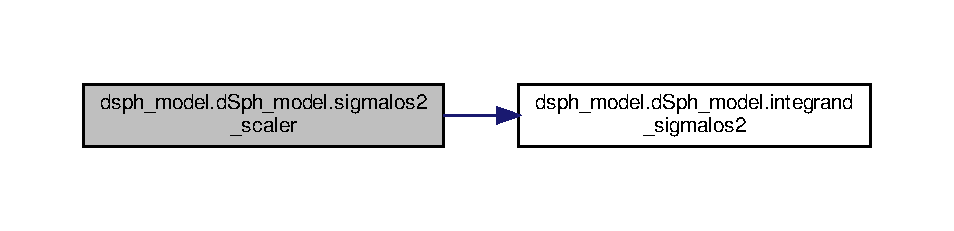
\includegraphics[width=350pt]{d0/d25/classdsph__model_1_1dSph__model_a05b988f7553121226a4d08369c44b4fa_cgraph}
\end{center}
\end{figure}
Here is the caller graph for this function\+:\nopagebreak
\begin{figure}[H]
\begin{center}
\leavevmode
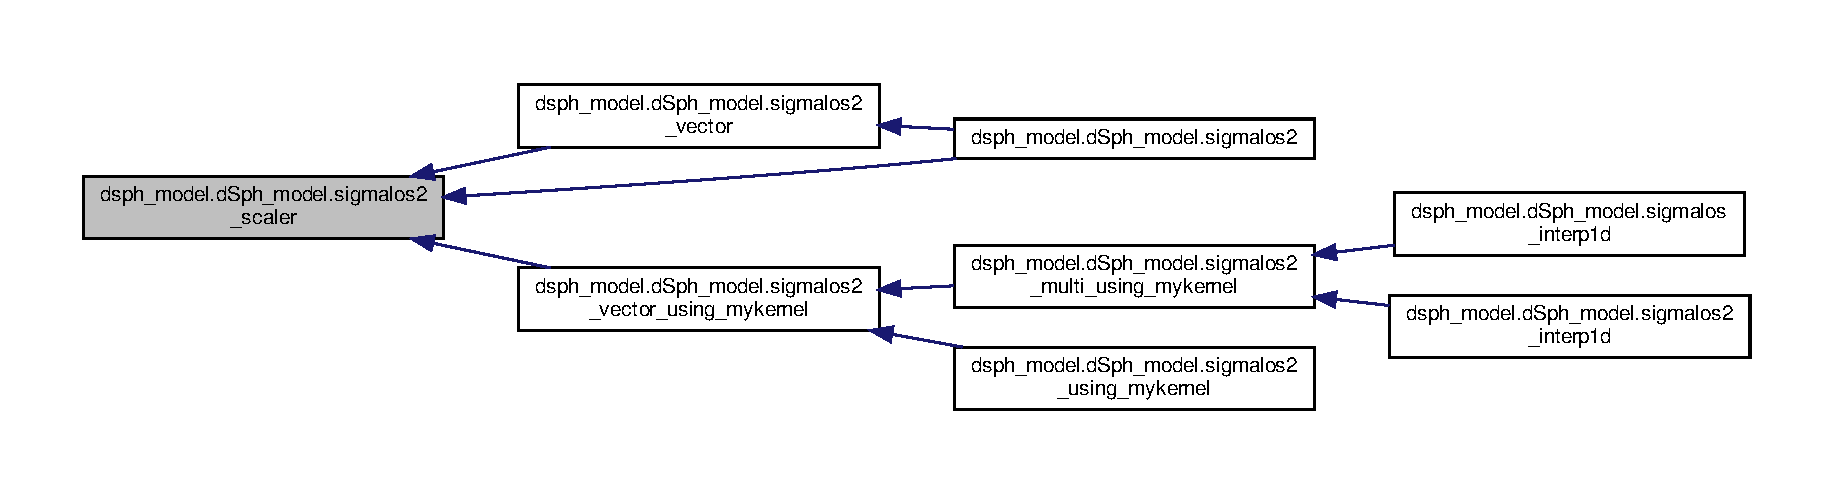
\includegraphics[width=350pt]{d0/d25/classdsph__model_1_1dSph__model_a05b988f7553121226a4d08369c44b4fa_icgraph}
\end{center}
\end{figure}
\mbox{\Hypertarget{classdsph__model_1_1dSph__model_a14692f81c0bffc790d5daf7f4e6464c1}\label{classdsph__model_1_1dSph__model_a14692f81c0bffc790d5daf7f4e6464c1}} 
\index{dsph\+\_\+model\+::d\+Sph\+\_\+model@{dsph\+\_\+model\+::d\+Sph\+\_\+model}!sigmalos2\+\_\+scaler\+\_\+using\+\_\+mykernel@{sigmalos2\+\_\+scaler\+\_\+using\+\_\+mykernel}}
\index{sigmalos2\+\_\+scaler\+\_\+using\+\_\+mykernel@{sigmalos2\+\_\+scaler\+\_\+using\+\_\+mykernel}!dsph\+\_\+model\+::d\+Sph\+\_\+model@{dsph\+\_\+model\+::d\+Sph\+\_\+model}}
\subsubsection{\texorpdfstring{sigmalos2\+\_\+scaler\+\_\+using\+\_\+mykernel()}{sigmalos2\_scaler\_using\_mykernel()}}
{\footnotesize\ttfamily def dsph\+\_\+model.\+d\+Sph\+\_\+model.\+sigmalos2\+\_\+scaler\+\_\+using\+\_\+mykernel (\begin{DoxyParamCaption}\item[{}]{self,  }\item[{}]{R\+\_\+pc }\end{DoxyParamCaption})}

\begin{DoxyVerb}sigmalos2[km^2 s^-2].
\end{DoxyVerb}
 

Definition at line 348 of file dsph\+\_\+model.\+py.


\begin{DoxyCode}
348     \textcolor{keyword}{def }sigmalos2\_scaler\_using\_mykernel(self,R\_pc):
349         \textcolor{stringliteral}{'''}
350 \textcolor{stringliteral}{        sigmalos2[km^2 s^-2].}
351 \textcolor{stringliteral}{        '''}
352         u\_trunc = self.submodels[\textcolor{stringliteral}{"DM\_model"}].params.R\_trunc\_pc/R\_pc
353         u\_max = 10 * u\_trunc
354         u\_re = self.submodels[\textcolor{stringliteral}{"stellar\_model"}].params.re\_pc/R\_pc
355 
356         \textcolor{comment}{# outer region is almost 0, so divede the region for good point -> u\_max}
357         
358         RELERR\_INTEG = 1e-6
359         integ, abserr =  integrate.quad(self.integrand\_sigmalos2\_using\_mykernel, 1,u\_max, args=(R\_pc,),
      points=(1.001,max(u\_re,1.08),2.71,u\_trunc))
360         \textcolor{keywordflow}{return} integ
361     
\end{DoxyCode}
Here is the call graph for this function\+:\nopagebreak
\begin{figure}[H]
\begin{center}
\leavevmode
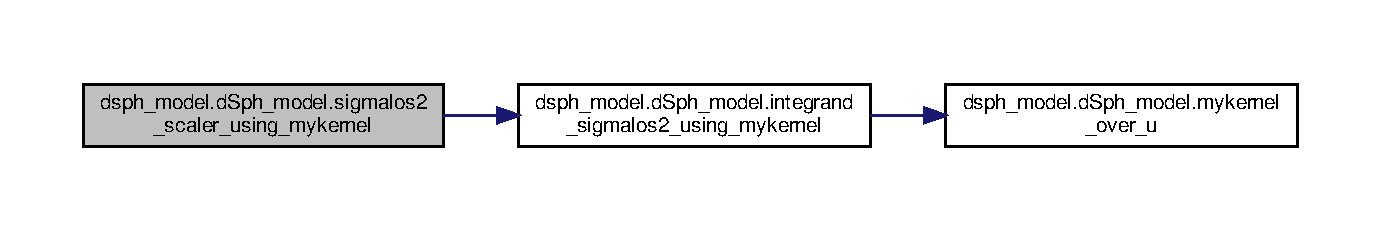
\includegraphics[width=350pt]{d0/d25/classdsph__model_1_1dSph__model_a14692f81c0bffc790d5daf7f4e6464c1_cgraph}
\end{center}
\end{figure}
Here is the caller graph for this function\+:\nopagebreak
\begin{figure}[H]
\begin{center}
\leavevmode
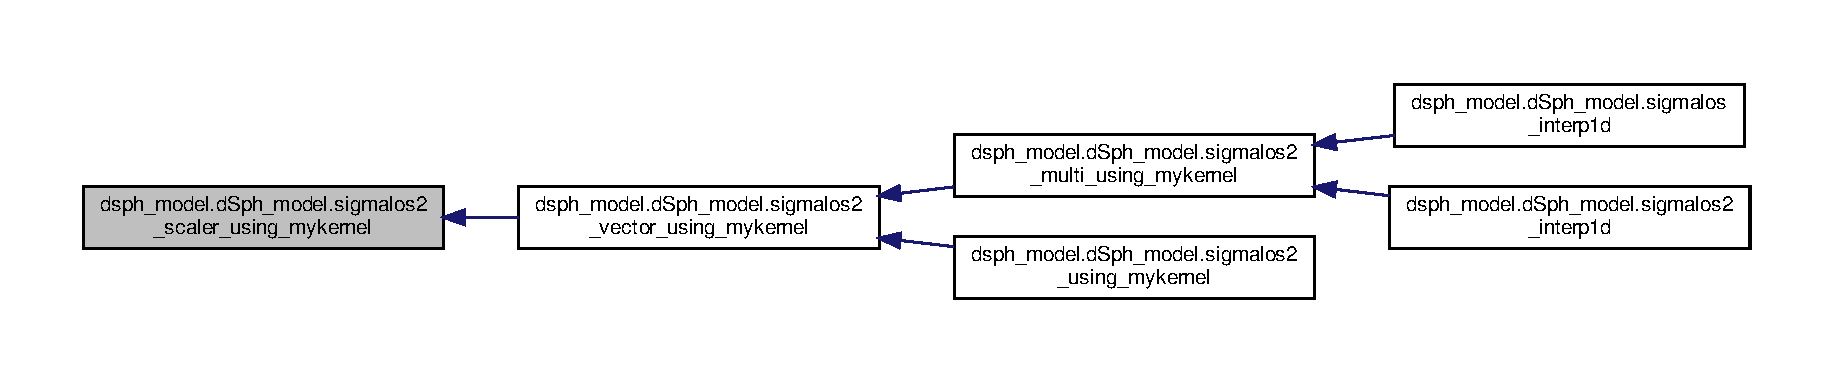
\includegraphics[width=350pt]{d0/d25/classdsph__model_1_1dSph__model_a14692f81c0bffc790d5daf7f4e6464c1_icgraph}
\end{center}
\end{figure}
\mbox{\Hypertarget{classdsph__model_1_1dSph__model_a4e062f0ac546057c1109fd47ec39ed90}\label{classdsph__model_1_1dSph__model_a4e062f0ac546057c1109fd47ec39ed90}} 
\index{dsph\+\_\+model\+::d\+Sph\+\_\+model@{dsph\+\_\+model\+::d\+Sph\+\_\+model}!sigmalos2\+\_\+using\+\_\+mykernel@{sigmalos2\+\_\+using\+\_\+mykernel}}
\index{sigmalos2\+\_\+using\+\_\+mykernel@{sigmalos2\+\_\+using\+\_\+mykernel}!dsph\+\_\+model\+::d\+Sph\+\_\+model@{dsph\+\_\+model\+::d\+Sph\+\_\+model}}
\subsubsection{\texorpdfstring{sigmalos2\+\_\+using\+\_\+mykernel()}{sigmalos2\_using\_mykernel()}}
{\footnotesize\ttfamily def dsph\+\_\+model.\+d\+Sph\+\_\+model.\+sigmalos2\+\_\+using\+\_\+mykernel (\begin{DoxyParamCaption}\item[{}]{self,  }\item[{}]{R\+\_\+pc }\end{DoxyParamCaption})}



Definition at line 442 of file dsph\+\_\+model.\+py.


\begin{DoxyCode}
442     \textcolor{keyword}{def }sigmalos2\_using\_mykernel(self,R\_pc):
443         \textcolor{keywordflow}{return} (self.sigmalos2\_scaler\_uging\_mykernel(R\_pc) \textcolor{keywordflow}{if} len(R\_pc)==1 \textcolor{keywordflow}{else} self.
      sigmalos2\_vector\_using\_mykernel(R\_pc))
444     
\end{DoxyCode}
Here is the call graph for this function\+:\nopagebreak
\begin{figure}[H]
\begin{center}
\leavevmode
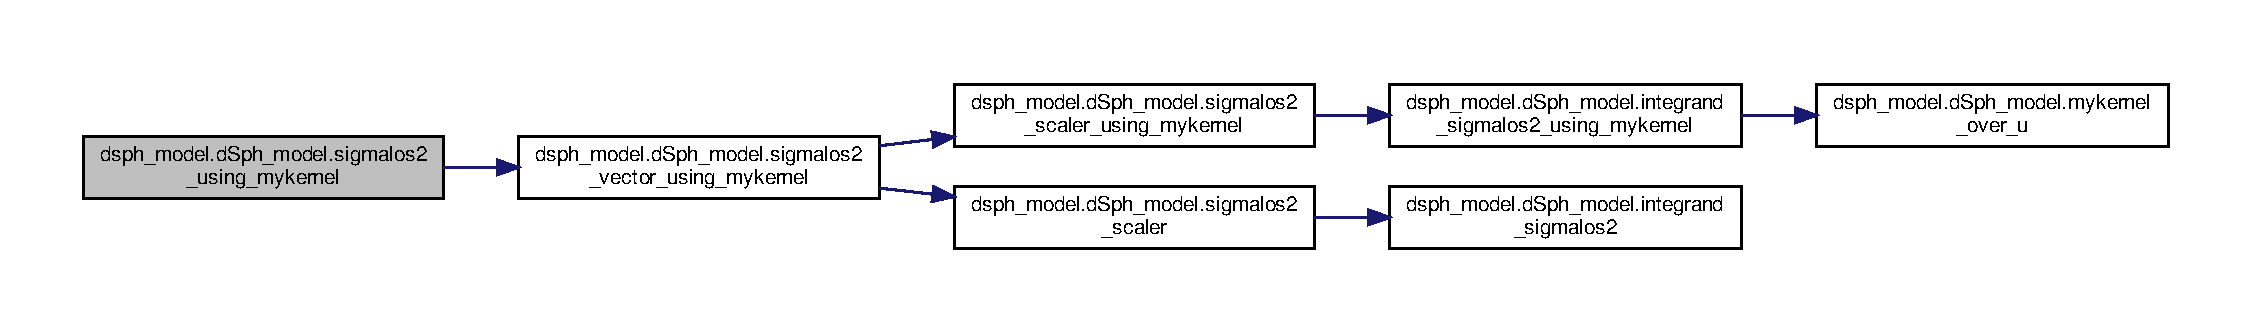
\includegraphics[width=350pt]{d0/d25/classdsph__model_1_1dSph__model_a4e062f0ac546057c1109fd47ec39ed90_cgraph}
\end{center}
\end{figure}
\mbox{\Hypertarget{classdsph__model_1_1dSph__model_a5170edb309402dc101ea76871645e65f}\label{classdsph__model_1_1dSph__model_a5170edb309402dc101ea76871645e65f}} 
\index{dsph\+\_\+model\+::d\+Sph\+\_\+model@{dsph\+\_\+model\+::d\+Sph\+\_\+model}!sigmalos2\+\_\+vector@{sigmalos2\+\_\+vector}}
\index{sigmalos2\+\_\+vector@{sigmalos2\+\_\+vector}!dsph\+\_\+model\+::d\+Sph\+\_\+model@{dsph\+\_\+model\+::d\+Sph\+\_\+model}}
\subsubsection{\texorpdfstring{sigmalos2\+\_\+vector()}{sigmalos2\_vector()}}
{\footnotesize\ttfamily def dsph\+\_\+model.\+d\+Sph\+\_\+model.\+sigmalos2\+\_\+vector (\begin{DoxyParamCaption}\item[{}]{self,  }\item[{}]{Rs\+\_\+pc }\end{DoxyParamCaption})}



Definition at line 423 of file dsph\+\_\+model.\+py.


\begin{DoxyCode}
423     \textcolor{keyword}{def }sigmalos2\_vector(self,Rs\_pc):
424         sigmalos2\_scaler = self.sigmalos2\_scaler
425         \textcolor{keywordflow}{return} [sigmalos2\_scaler(R\_pc) \textcolor{keywordflow}{for} R\_pc \textcolor{keywordflow}{in} Rs\_pc]
426     
\end{DoxyCode}
Here is the call graph for this function\+:\nopagebreak
\begin{figure}[H]
\begin{center}
\leavevmode
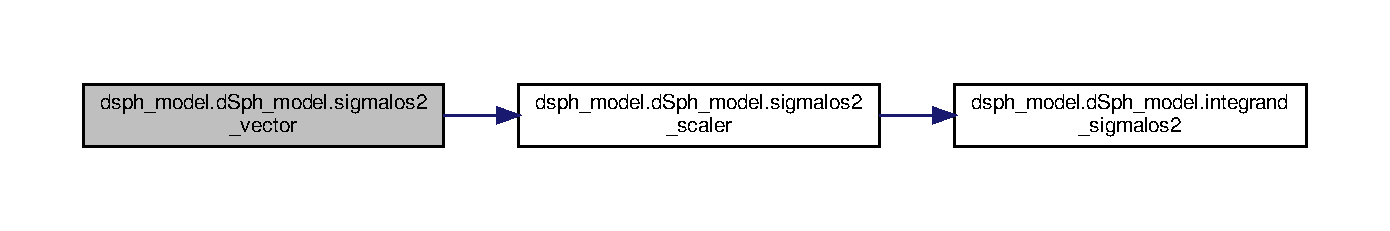
\includegraphics[width=350pt]{d0/d25/classdsph__model_1_1dSph__model_a5170edb309402dc101ea76871645e65f_cgraph}
\end{center}
\end{figure}
Here is the caller graph for this function\+:\nopagebreak
\begin{figure}[H]
\begin{center}
\leavevmode
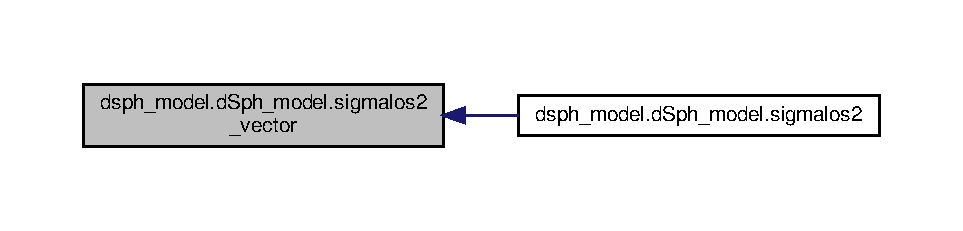
\includegraphics[width=350pt]{d0/d25/classdsph__model_1_1dSph__model_a5170edb309402dc101ea76871645e65f_icgraph}
\end{center}
\end{figure}
\mbox{\Hypertarget{classdsph__model_1_1dSph__model_a00cd796cf178fe8b3435e941976e8f27}\label{classdsph__model_1_1dSph__model_a00cd796cf178fe8b3435e941976e8f27}} 
\index{dsph\+\_\+model\+::d\+Sph\+\_\+model@{dsph\+\_\+model\+::d\+Sph\+\_\+model}!sigmalos2\+\_\+vector\+\_\+using\+\_\+mykernel@{sigmalos2\+\_\+vector\+\_\+using\+\_\+mykernel}}
\index{sigmalos2\+\_\+vector\+\_\+using\+\_\+mykernel@{sigmalos2\+\_\+vector\+\_\+using\+\_\+mykernel}!dsph\+\_\+model\+::d\+Sph\+\_\+model@{dsph\+\_\+model\+::d\+Sph\+\_\+model}}
\subsubsection{\texorpdfstring{sigmalos2\+\_\+vector\+\_\+using\+\_\+mykernel()}{sigmalos2\_vector\_using\_mykernel()}}
{\footnotesize\ttfamily def dsph\+\_\+model.\+d\+Sph\+\_\+model.\+sigmalos2\+\_\+vector\+\_\+using\+\_\+mykernel (\begin{DoxyParamCaption}\item[{}]{self,  }\item[{}]{Rs\+\_\+pc }\end{DoxyParamCaption})}



Definition at line 427 of file dsph\+\_\+model.\+py.


\begin{DoxyCode}
427     \textcolor{keyword}{def }sigmalos2\_vector\_using\_mykernel(self,Rs\_pc):
428         sigmalos2\_scaler = self.sigmalos2\_scaler\_using\_mykernel
429         \textcolor{keywordflow}{return} [sigmalos2\_scaler(R\_pc) \textcolor{keywordflow}{for} R\_pc \textcolor{keywordflow}{in} Rs\_pc]
430     
\end{DoxyCode}
Here is the call graph for this function\+:\nopagebreak
\begin{figure}[H]
\begin{center}
\leavevmode
\includegraphics[width=350pt]{d0/d25/classdsph__model_1_1dSph__model_a00cd796cf178fe8b3435e941976e8f27_cgraph}
\end{center}
\end{figure}
Here is the caller graph for this function\+:\nopagebreak
\begin{figure}[H]
\begin{center}
\leavevmode
\includegraphics[width=350pt]{d0/d25/classdsph__model_1_1dSph__model_a00cd796cf178fe8b3435e941976e8f27_icgraph}
\end{center}
\end{figure}
\mbox{\Hypertarget{classdsph__model_1_1dSph__model_a5b73e854e8ac1b1c6a467498cd181e7a}\label{classdsph__model_1_1dSph__model_a5b73e854e8ac1b1c6a467498cd181e7a}} 
\index{dsph\+\_\+model\+::d\+Sph\+\_\+model@{dsph\+\_\+model\+::d\+Sph\+\_\+model}!sigmalos\+\_\+dequad@{sigmalos\+\_\+dequad}}
\index{sigmalos\+\_\+dequad@{sigmalos\+\_\+dequad}!dsph\+\_\+model\+::d\+Sph\+\_\+model@{dsph\+\_\+model\+::d\+Sph\+\_\+model}}
\subsubsection{\texorpdfstring{sigmalos\+\_\+dequad()}{sigmalos\_dequad()}}
{\footnotesize\ttfamily def dsph\+\_\+model.\+d\+Sph\+\_\+model.\+sigmalos\+\_\+dequad (\begin{DoxyParamCaption}\item[{}]{self,  }\item[{}]{R\+\_\+pc,  }\item[{}]{show\+\_\+fig = {\ttfamily False},  }\item[{}]{dtype = {\ttfamily np.float64},  }\item[{}]{ignore\+\_\+nan = {\ttfamily False} }\end{DoxyParamCaption})}



Definition at line 372 of file dsph\+\_\+model.\+py.


\begin{DoxyCode}
372     \textcolor{keyword}{def }sigmalos\_dequad(self,R\_pc,show\_fig=False,dtype=np.float64,ignore\_nan=False):
373         \textcolor{keyword}{def }func(u):
374             u\_ = np.array(u)[np.newaxis,:]
375             R\_pc\_ = np.array(R\_pc)[:,np.newaxis]
376             \textcolor{keywordflow}{return} self.integrand\_sigmalos2\_using\_mykernel(u\_,R\_pc\_)
377         \textcolor{keywordflow}{return} np.sqrt(\hyperlink{namespacedequad}{dequad}(func,1,inf,axis=1,width=5e-3,pN=1000,mN=1000,dtype=dtype,show\_fig=
      show\_fig,ignore\_nan=ignore\_nan))
378     
\end{DoxyCode}
Here is the call graph for this function\+:\nopagebreak
\begin{figure}[H]
\begin{center}
\leavevmode
\includegraphics[width=350pt]{d0/d25/classdsph__model_1_1dSph__model_a5b73e854e8ac1b1c6a467498cd181e7a_cgraph}
\end{center}
\end{figure}
Here is the caller graph for this function\+:\nopagebreak
\begin{figure}[H]
\begin{center}
\leavevmode
\includegraphics[width=350pt]{d0/d25/classdsph__model_1_1dSph__model_a5b73e854e8ac1b1c6a467498cd181e7a_icgraph}
\end{center}
\end{figure}
\mbox{\Hypertarget{classdsph__model_1_1dSph__model_a0046cd7677792835d8cfafe83dbe276c}\label{classdsph__model_1_1dSph__model_a0046cd7677792835d8cfafe83dbe276c}} 
\index{dsph\+\_\+model\+::d\+Sph\+\_\+model@{dsph\+\_\+model\+::d\+Sph\+\_\+model}!sigmalos\+\_\+dequad\+\_\+interp1d\+\_\+downsampled@{sigmalos\+\_\+dequad\+\_\+interp1d\+\_\+downsampled}}
\index{sigmalos\+\_\+dequad\+\_\+interp1d\+\_\+downsampled@{sigmalos\+\_\+dequad\+\_\+interp1d\+\_\+downsampled}!dsph\+\_\+model\+::d\+Sph\+\_\+model@{dsph\+\_\+model\+::d\+Sph\+\_\+model}}
\subsubsection{\texorpdfstring{sigmalos\+\_\+dequad\+\_\+interp1d\+\_\+downsampled()}{sigmalos\_dequad\_interp1d\_downsampled()}}
{\footnotesize\ttfamily def dsph\+\_\+model.\+d\+Sph\+\_\+model.\+sigmalos\+\_\+dequad\+\_\+interp1d\+\_\+downsampled (\begin{DoxyParamCaption}\item[{}]{self,  }\item[{}]{R\+\_\+pc,  }\item[{}]{downsampling\+\_\+rate = {\ttfamily 0.6},  }\item[{}]{iteration = {\ttfamily 5},  }\item[{}]{kind = {\ttfamily \char`\"{}cubic\char`\"{}},  }\item[{}]{offset = {\ttfamily 5},  }\item[{}]{sep\+\_\+offset = {\ttfamily 1},  }\item[{}]{points = {\ttfamily \mbox{[}25.},  }\item[{}]{show\+\_\+fig = {\ttfamily False},  }\item[{}]{dtype = {\ttfamily np.float64},  }\item[{}]{ignore\+\_\+nan = {\ttfamily True} }\end{DoxyParamCaption})}



Definition at line 402 of file dsph\+\_\+model.\+py.


\begin{DoxyCode}
402     \textcolor{keyword}{def }sigmalos\_dequad\_interp1d\_downsampled(
      self,R\_pc,downsampling\_rate=0.6,iteration=5,kind="cubic",offset
      =5,sep\_offset=1,points=[25.,50.,100.,191.,400.,1950.,2000.,2050.],show\_fig=False,dtype=np.float64,ignore\_nan=True):
403         R\_pc\_sorted = sort(R\_pc)
404         R\_pc\_downsampled = np.unique(np.concatenate([self.downsamplings(R\_pc,iteration=iteration),
      R\_pc\_sorted[:offset:sep\_offset],R\_pc\_sorted[-offset::sep\_offset],points]))
405         sigmalos\_ = self.sigmalos\_dequad(R\_pc\_downsampled,show\_fig=show\_fig,dtype=dtype,ignore\_nan=
      ignore\_nan)
406         interpd\_func = interp1d(R\_pc\_downsampled, sigmalos\_,kind=kind)
407         \textcolor{comment}{#interpd\_func = Akima1DInterpolator(R\_pc\_downsampled, sigmalos\_)}
408         \textcolor{keywordflow}{return} interpd\_func(R\_pc) \textcolor{comment}{# here R\_pc is original, so return unsorted results}
409         
410     
\end{DoxyCode}
Here is the call graph for this function\+:\nopagebreak
\begin{figure}[H]
\begin{center}
\leavevmode
\includegraphics[width=350pt]{d0/d25/classdsph__model_1_1dSph__model_a0046cd7677792835d8cfafe83dbe276c_cgraph}
\end{center}
\end{figure}
\mbox{\Hypertarget{classdsph__model_1_1dSph__model_ad105b90e1827d25804eb3d7a3ba96f28}\label{classdsph__model_1_1dSph__model_ad105b90e1827d25804eb3d7a3ba96f28}} 
\index{dsph\+\_\+model\+::d\+Sph\+\_\+model@{dsph\+\_\+model\+::d\+Sph\+\_\+model}!sigmalos\+\_\+interp1d@{sigmalos\+\_\+interp1d}}
\index{sigmalos\+\_\+interp1d@{sigmalos\+\_\+interp1d}!dsph\+\_\+model\+::d\+Sph\+\_\+model@{dsph\+\_\+model\+::d\+Sph\+\_\+model}}
\subsubsection{\texorpdfstring{sigmalos\+\_\+interp1d()}{sigmalos\_interp1d()}}
{\footnotesize\ttfamily def dsph\+\_\+model.\+d\+Sph\+\_\+model.\+sigmalos\+\_\+interp1d (\begin{DoxyParamCaption}\item[{}]{self,  }\item[{}]{R\+\_\+pc,  }\item[{}]{dR = {\ttfamily 1},  }\item[{}]{d\+Rtrunc = {\ttfamily 10},  }\item[{}]{step\+\_\+around\+\_\+\+Rtrunc = {\ttfamily 10},  }\item[{}]{step\+\_\+outer = {\ttfamily 8},  }\item[{}]{step\+\_\+center = {\ttfamily 4},  }\item[{}]{kind = {\ttfamily \char`\"{}cubic\char`\"{}} }\end{DoxyParamCaption})}

\begin{DoxyVerb}inner part has large error, so more refine interp
\end{DoxyVerb}
 

Definition at line 445 of file dsph\+\_\+model.\+py.


\begin{DoxyCode}
445     \textcolor{keyword}{def }sigmalos\_interp1d(
      self,R\_pc,dR=1,dRtrunc=10,step\_around\_Rtrunc=10,step\_outer=8,step\_center=4,kind="cubic"):
446         \textcolor{stringliteral}{'''}
447 \textcolor{stringliteral}{        inner part has large error, so more refine interp}
448 \textcolor{stringliteral}{        '''}
449         re = self.submodels[\textcolor{stringliteral}{"stellar\_model"}].params.re\_pc
450         Rtrunc = self.submodels[\textcolor{stringliteral}{"DM\_model"}].params.R\_trunc\_pc
451         n = len(R\_pc)
452         R\_pc\_sorted\_ = np.sort(R\_pc)
453         R\_pc\_around\_Rtrunc = np.sort(R\_pc\_sorted\_[np.argsort(np.abs(R\_pc\_sorted\_-Rtrunc))[:
      step\_around\_Rtrunc]])
454         Rmin,Rmax = R\_pc\_sorted\_[0],R\_pc\_sorted\_[-1]
455         \textcolor{comment}{#R\_pc\_lo\_ = np.linspace(Rmin*0.5,Rmin*1.5,int((n*0.2)/step))}
456         \textcolor{comment}{#R\_pc\_lo\_ = R\_pc\_sorted\_[:int(n*0.05)]}
457         \textcolor{comment}{#R\_pc\_hi\_ = np.linspace(R\_pc\_lo\_[-1]+0.1,Rmax*1.1,int(n/step))}
458         \textcolor{comment}{#R\_pc\_ = np.hstack((R\_pc\_lo\_,R\_pc\_hi\_))}
459         R\_pc\_zero = R\_pc\_sorted\_[:step\_center]
460         R\_pc\_hi\_ = np.logspace(np.log10(R\_pc\_sorted\_[step\_center]),np.log10(Rmax)+1e-8,step\_outer)
461         R\_pc\_ = np.sort(np.unique(np.concatenate((R\_pc\_zero,R\_pc\_around\_Rtrunc,R\_pc\_hi\_),axis=\textcolor{keywordtype}{None})))
462         \textcolor{comment}{#R\_pc\_ = np.linspace(Rmin,Rmax,int(n/step))}
463         sigmalos2\_ = self.sigmalos2\_multi\_using\_mykernel(R\_pc\_)
464         interpd\_func = interp1d(R\_pc\_, sqrt(sigmalos2\_),kind=kind)
465         \textcolor{keywordflow}{return} interpd\_func(R\_pc) \textcolor{comment}{# here R\_pc is original, so return unsorted results}
466     
\end{DoxyCode}
Here is the call graph for this function\+:\nopagebreak
\begin{figure}[H]
\begin{center}
\leavevmode
\includegraphics[width=350pt]{d0/d25/classdsph__model_1_1dSph__model_ad105b90e1827d25804eb3d7a3ba96f28_cgraph}
\end{center}
\end{figure}
\mbox{\Hypertarget{classdsph__model_1_1dSph__model_a239ec859750c30fe31b6c19e94cd2e33}\label{classdsph__model_1_1dSph__model_a239ec859750c30fe31b6c19e94cd2e33}} 
\index{dsph\+\_\+model\+::d\+Sph\+\_\+model@{dsph\+\_\+model\+::d\+Sph\+\_\+model}!sigmalos\+\_\+interp1d\+\_\+dequad@{sigmalos\+\_\+interp1d\+\_\+dequad}}
\index{sigmalos\+\_\+interp1d\+\_\+dequad@{sigmalos\+\_\+interp1d\+\_\+dequad}!dsph\+\_\+model\+::d\+Sph\+\_\+model@{dsph\+\_\+model\+::d\+Sph\+\_\+model}}
\subsubsection{\texorpdfstring{sigmalos\+\_\+interp1d\+\_\+dequad()}{sigmalos\_interp1d\_dequad()}}
{\footnotesize\ttfamily def dsph\+\_\+model.\+d\+Sph\+\_\+model.\+sigmalos\+\_\+interp1d\+\_\+dequad (\begin{DoxyParamCaption}\item[{}]{self,  }\item[{}]{R\+\_\+pc,  }\item[{}]{dR = {\ttfamily 1},  }\item[{}]{d\+Rtrunc = {\ttfamily 10},  }\item[{}]{step\+\_\+around\+\_\+\+Rtrunc = {\ttfamily 10},  }\item[{}]{step\+\_\+outer = {\ttfamily 20},  }\item[{}]{step\+\_\+center = {\ttfamily 4},  }\item[{}]{kind = {\ttfamily \char`\"{}cubic\char`\"{}} }\end{DoxyParamCaption})}

\begin{DoxyVerb}inner part has large error, so more refine interp
\end{DoxyVerb}
 

Definition at line 467 of file dsph\+\_\+model.\+py.


\begin{DoxyCode}
467     \textcolor{keyword}{def }sigmalos\_interp1d\_dequad(
      self,R\_pc,dR=1,dRtrunc=10,step\_around\_Rtrunc=10,step\_outer=20,step\_center=4,kind="cubic"):
468         \textcolor{stringliteral}{'''}
469 \textcolor{stringliteral}{        inner part has large error, so more refine interp}
470 \textcolor{stringliteral}{        '''}
471         re = self.submodels[\textcolor{stringliteral}{"stellar\_model"}].params.re\_pc
472         Rtrunc = self.submodels[\textcolor{stringliteral}{"DM\_model"}].params.R\_trunc\_pc
473         n = len(R\_pc)
474         R\_pc\_sorted\_ = np.sort(R\_pc)
475         R\_pc\_around\_Rtrunc = np.sort(R\_pc\_sorted\_[np.argsort(np.abs(R\_pc\_sorted\_-Rtrunc))[:
      step\_around\_Rtrunc]])
476         Rmin,Rmax = R\_pc\_sorted\_[0],R\_pc\_sorted\_[-1]
477         \textcolor{comment}{#R\_pc\_lo\_ = np.linspace(Rmin*0.5,Rmin*1.5,int((n*0.2)/step))}
478         \textcolor{comment}{#R\_pc\_lo\_ = R\_pc\_sorted\_[:int(n*0.05)]}
479         \textcolor{comment}{#R\_pc\_hi\_ = np.linspace(R\_pc\_lo\_[-1]+0.1,Rmax*1.1,int(n/step))}
480         \textcolor{comment}{#R\_pc\_ = np.hstack((R\_pc\_lo\_,R\_pc\_hi\_))}
481         R\_pc\_zero = R\_pc\_sorted\_[:step\_center]
482         R\_pc\_hi\_ = np.logspace(np.log10(R\_pc\_sorted\_[step\_center]),np.log10(Rmax)+1e-8,step\_outer)
483         R\_pc\_ = np.sort(np.unique(np.concatenate((R\_pc\_zero,R\_pc\_around\_Rtrunc,R\_pc\_hi\_),axis=\textcolor{keywordtype}{None})))
484         \textcolor{comment}{#R\_pc\_ = np.linspace(Rmin,Rmax,int(n/step))}
485         sigmalos2\_ = self.sigmalos2\_dequad(R\_pc\_)
486         interpd\_func = interp1d(R\_pc\_, sqrt(sigmalos2\_),kind=kind)
487         \textcolor{keywordflow}{return} interpd\_func(R\_pc) \textcolor{comment}{# here R\_pc is original, so return unsorted results}
488     
\end{DoxyCode}
Here is the call graph for this function\+:\nopagebreak
\begin{figure}[H]
\begin{center}
\leavevmode
\includegraphics[width=350pt]{d0/d25/classdsph__model_1_1dSph__model_a239ec859750c30fe31b6c19e94cd2e33_cgraph}
\end{center}
\end{figure}
\mbox{\Hypertarget{classdsph__model_1_1dSph__model_a1c6185c02a3f58951b7ed9b75a348f49}\label{classdsph__model_1_1dSph__model_a1c6185c02a3f58951b7ed9b75a348f49}} 
\index{dsph\+\_\+model\+::d\+Sph\+\_\+model@{dsph\+\_\+model\+::d\+Sph\+\_\+model}!sigmar2@{sigmar2}}
\index{sigmar2@{sigmar2}!dsph\+\_\+model\+::d\+Sph\+\_\+model@{dsph\+\_\+model\+::d\+Sph\+\_\+model}}
\subsubsection{\texorpdfstring{sigmar2()}{sigmar2()}}
{\footnotesize\ttfamily def dsph\+\_\+model.\+d\+Sph\+\_\+model.\+sigmar2 (\begin{DoxyParamCaption}\item[{}]{self,  }\item[{}]{r\+\_\+pc }\end{DoxyParamCaption})}



Definition at line 299 of file dsph\+\_\+model.\+py.


\begin{DoxyCode}
299     \textcolor{keyword}{def }sigmar2(self,r\_pc):
300         RELERROR\_INTEG = 1e-6
301         anib = self.params.anib
302         integrand = \textcolor{keyword}{lambda} r,r1: self.submodels[\textcolor{stringliteral}{"stellar\_model"}].density\_3d(r)*np.power(r/r1,-2*anib)*
      GMsun\_m3s2*self.submodels[\textcolor{stringliteral}{"DM\_model"}].enclosure\_mass(r)/r**2/self.submodels[\textcolor{stringliteral}{"stellar\_model"}].density\_3d(r\_pc)*1e-
      6/parsec
303         integ, abserr = integrate.quad(integrand,r\_pc,np.inf,args=(r\_pc,))
304         \textcolor{keywordflow}{return} integ
305     
\end{DoxyCode}
Here is the caller graph for this function\+:\nopagebreak
\begin{figure}[H]
\begin{center}
\leavevmode
\includegraphics[width=350pt]{d0/d25/classdsph__model_1_1dSph__model_a1c6185c02a3f58951b7ed9b75a348f49_icgraph}
\end{center}
\end{figure}


\subsection{Member Data Documentation}
\mbox{\Hypertarget{classdsph__model_1_1dSph__model_a44e4805fa7304536056b19bd361c3d37}\label{classdsph__model_1_1dSph__model_a44e4805fa7304536056b19bd361c3d37}} 
\index{dsph\+\_\+model\+::d\+Sph\+\_\+model@{dsph\+\_\+model\+::d\+Sph\+\_\+model}!name@{name}}
\index{name@{name}!dsph\+\_\+model\+::d\+Sph\+\_\+model@{dsph\+\_\+model\+::d\+Sph\+\_\+model}}
\subsubsection{\texorpdfstring{name}{name}}
{\footnotesize\ttfamily string dsph\+\_\+model.\+d\+Sph\+\_\+model.\+name = \textquotesingle{}\hyperlink{classdsph__model_1_1dSph__model}{d\+Sph\+\_\+model}\textquotesingle{}\hspace{0.3cm}{\ttfamily [static]}}



Definition at line 272 of file dsph\+\_\+model.\+py.

\mbox{\Hypertarget{classdsph__model_1_1dSph__model_ab09f579bff6269075f5956a1c0a88bdc}\label{classdsph__model_1_1dSph__model_ab09f579bff6269075f5956a1c0a88bdc}} 
\index{dsph\+\_\+model\+::d\+Sph\+\_\+model@{dsph\+\_\+model\+::d\+Sph\+\_\+model}!ncpu@{ncpu}}
\index{ncpu@{ncpu}!dsph\+\_\+model\+::d\+Sph\+\_\+model@{dsph\+\_\+model\+::d\+Sph\+\_\+model}}
\subsubsection{\texorpdfstring{ncpu}{ncpu}}
{\footnotesize\ttfamily dsph\+\_\+model.\+d\+Sph\+\_\+model.\+ncpu = multi.\+cpu\+\_\+count()\hspace{0.3cm}{\ttfamily [static]}}



Definition at line 275 of file dsph\+\_\+model.\+py.

\mbox{\Hypertarget{classdsph__model_1_1dSph__model_a7795b8e9d3d0dbf3cd5a4d618c30a6c0}\label{classdsph__model_1_1dSph__model_a7795b8e9d3d0dbf3cd5a4d618c30a6c0}} 
\index{dsph\+\_\+model\+::d\+Sph\+\_\+model@{dsph\+\_\+model\+::d\+Sph\+\_\+model}!required\+\_\+models@{required\+\_\+models}}
\index{required\+\_\+models@{required\+\_\+models}!dsph\+\_\+model\+::d\+Sph\+\_\+model@{dsph\+\_\+model\+::d\+Sph\+\_\+model}}
\subsubsection{\texorpdfstring{required\+\_\+models}{required\_models}}
{\footnotesize\ttfamily list dsph\+\_\+model.\+d\+Sph\+\_\+model.\+required\+\_\+models = \mbox{[}\hyperlink{classdsph__model_1_1stellar__model}{stellar\+\_\+model},\hyperlink{classdsph__model_1_1DM__model}{D\+M\+\_\+model}\mbox{]}\hspace{0.3cm}{\ttfamily [static]}}



Definition at line 274 of file dsph\+\_\+model.\+py.

\mbox{\Hypertarget{classdsph__model_1_1dSph__model_a74f031f3929b9123b00121c1b02b8b71}\label{classdsph__model_1_1dSph__model_a74f031f3929b9123b00121c1b02b8b71}} 
\index{dsph\+\_\+model\+::d\+Sph\+\_\+model@{dsph\+\_\+model\+::d\+Sph\+\_\+model}!required\+\_\+params\+\_\+name@{required\+\_\+params\+\_\+name}}
\index{required\+\_\+params\+\_\+name@{required\+\_\+params\+\_\+name}!dsph\+\_\+model\+::d\+Sph\+\_\+model@{dsph\+\_\+model\+::d\+Sph\+\_\+model}}
\subsubsection{\texorpdfstring{required\+\_\+params\+\_\+name}{required\_params\_name}}
{\footnotesize\ttfamily list dsph\+\_\+model.\+d\+Sph\+\_\+model.\+required\+\_\+params\+\_\+name = \mbox{[}\textquotesingle{}anib\textquotesingle{}\mbox{]}\hspace{0.3cm}{\ttfamily [static]}}



Definition at line 273 of file dsph\+\_\+model.\+py.



The documentation for this class was generated from the following file\+:\begin{DoxyCompactItemize}
\item 
memfg/\hyperlink{dsph__model_8py}{dsph\+\_\+model.\+py}\end{DoxyCompactItemize}

\hypertarget{classdsphdata_1_1dSphData}{}\section{dsphdata.\+d\+Sph\+Data Class Reference}
\label{classdsphdata_1_1dSphData}\index{dsphdata.\+d\+Sph\+Data@{dsphdata.\+d\+Sph\+Data}}


Collaboration diagram for dsphdata.\+d\+Sph\+Data\+:\nopagebreak
\begin{figure}[H]
\begin{center}
\leavevmode
\includegraphics[width=183pt]{da/d49/classdsphdata_1_1dSphData__coll__graph}
\end{center}
\end{figure}
\subsection*{Public Member Functions}
\begin{DoxyCompactItemize}
\item 
def \hyperlink{classdsphdata_1_1dSphData_afcd54ca5255be74de80578f5962daba8}{\+\_\+\+\_\+init\+\_\+\+\_\+} (self, fname\+\_\+photo=None, fname\+\_\+spec=None, idx\+\_\+photo=None, idx\+\_\+spec=None)
\item 
def \hyperlink{classdsphdata_1_1dSphData_a582365655d5493e34b14c2697e79c4fe}{load\+\_\+csv} (self, name, fname, index\+\_\+col=None, cut=None, ra\+\_\+idx=\char`\"{}ra\char`\"{}, dec\+\_\+idx=\char`\"{}dec\char`\"{}, radial\+\_\+velocity\+\_\+idx=None, radial\+\_\+velocity\+\_\+err\+\_\+idx=None)
\item 
def \hyperlink{classdsphdata_1_1dSphData_a5384bafd3c725eb6c324664c7b47eae1}{to\+\_\+sc} (self, which)
\end{DoxyCompactItemize}
\subsection*{Static Public Attributes}
\begin{DoxyCompactItemize}
\item 
\hyperlink{classdsphdata_1_1dSphData_a1ebfbfbd27ed84f68b401606530c35ef}{idx\+\_\+photo\+\_\+default} = dict(index\+\_\+col=0,cut=\char`\"{}in\+\_\+cmdcut\char`\"{},ra\+\_\+idx=\char`\"{}ra\+Mean\char`\"{},dec\+\_\+idx=\char`\"{}dec\+Mean\char`\"{})
\item 
\hyperlink{classdsphdata_1_1dSphData_aaebb5308a014e2064f325f1897ae366a}{idx\+\_\+spec\+\_\+default} = dict(index\+\_\+col=0,cut=\char`\"{}in\+\_\+cmdcut\char`\"{},ra\+\_\+idx=\char`\"{}ra\char`\"{}, dec\+\_\+idx=\char`\"{}dec\char`\"{},radial\+\_\+velocity\+\_\+idx=\char`\"{}v\+\_\+helio\char`\"{},radial\+\_\+velocity\+\_\+err\+\_\+idx=\char`\"{}err\+\_\+v\+\_\+helio\char`\"{})
\end{DoxyCompactItemize}


\subsection{Detailed Description}
\begin{DoxyVerb}data class of the observed data of dSph.

attributes:
    - \end{DoxyVerb}
 

Definition at line 38 of file dsphdata.\+py.



\subsection{Constructor \& Destructor Documentation}
\mbox{\Hypertarget{classdsphdata_1_1dSphData_afcd54ca5255be74de80578f5962daba8}\label{classdsphdata_1_1dSphData_afcd54ca5255be74de80578f5962daba8}} 
\index{dsphdata\+::d\+Sph\+Data@{dsphdata\+::d\+Sph\+Data}!\+\_\+\+\_\+init\+\_\+\+\_\+@{\+\_\+\+\_\+init\+\_\+\+\_\+}}
\index{\+\_\+\+\_\+init\+\_\+\+\_\+@{\+\_\+\+\_\+init\+\_\+\+\_\+}!dsphdata\+::d\+Sph\+Data@{dsphdata\+::d\+Sph\+Data}}
\subsubsection{\texorpdfstring{\+\_\+\+\_\+init\+\_\+\+\_\+()}{\_\_init\_\_()}}
{\footnotesize\ttfamily def dsphdata.\+d\+Sph\+Data.\+\_\+\+\_\+init\+\_\+\+\_\+ (\begin{DoxyParamCaption}\item[{}]{self,  }\item[{}]{fname\+\_\+photo = {\ttfamily None},  }\item[{}]{fname\+\_\+spec = {\ttfamily None},  }\item[{}]{idx\+\_\+photo = {\ttfamily None},  }\item[{}]{idx\+\_\+spec = {\ttfamily None} }\end{DoxyParamCaption})}

\begin{DoxyVerb}initialize a sampler instance.

input:
    - dsph_name(str)   : dwarf spheroidal name listed in "Nearbygalaxies.dat".
    - fname_photo(str) : file name of photometry data
    - fname_spec(str)  : file name of spectroscopy data
    - idx_photo,idx_spec(dict) : dictionary of argument passed to "self.load_file".
\end{DoxyVerb}
 

Definition at line 51 of file dsphdata.\+py.


\begin{DoxyCode}
51                  idx\_photo=\textcolor{keywordtype}{None},idx\_spec=\textcolor{keywordtype}{None}):
52         \textcolor{stringliteral}{'''}
53 \textcolor{stringliteral}{        initialize a sampler instance.}
54 \textcolor{stringliteral}{        }
55 \textcolor{stringliteral}{        input:}
56 \textcolor{stringliteral}{            - dsph\_name(str)   : dwarf spheroidal name listed in "Nearbygalaxies.dat".}
57 \textcolor{stringliteral}{            - fname\_photo(str) : file name of photometry data}
58 \textcolor{stringliteral}{            - fname\_spec(str)  : file name of spectroscopy data}
59 \textcolor{stringliteral}{            - idx\_photo,idx\_spec(dict) : dictionary of argument passed to "self.load\_file".}
60 \textcolor{stringliteral}{        '''}
61         idx\_photo = dSphData.idx\_photo\_default \textcolor{keywordflow}{if} idx\_photo \textcolor{keywordflow}{is} \textcolor{keywordtype}{None} \textcolor{keywordflow}{else} idx\_photo
62         idx\_spec = dSphData.idx\_spec\_default \textcolor{keywordflow}{if} idx\_spec \textcolor{keywordflow}{is} \textcolor{keywordtype}{None} \textcolor{keywordflow}{else} idx\_spec
63 
64         \textcolor{keywordflow}{if} \textcolor{keywordflow}{not} fname\_photo \textcolor{keywordflow}{is} \textcolor{keywordtype}{None}:
65             self.load\_csv(\textcolor{stringliteral}{"photo"},fname\_photo,**idx\_photo)
66         \textcolor{keywordflow}{if} \textcolor{keywordflow}{not}  fname\_spec \textcolor{keywordflow}{is} \textcolor{keywordtype}{None}:
67             self.load\_csv(\textcolor{stringliteral}{"spec"}, fname\_spec, **idx\_spec)
68         
\end{DoxyCode}
Here is the call graph for this function\+:\nopagebreak
\begin{figure}[H]
\begin{center}
\leavevmode
\includegraphics[width=350pt]{d1/dbc/classdsphdata_1_1dSphData_afcd54ca5255be74de80578f5962daba8_cgraph}
\end{center}
\end{figure}


\subsection{Member Function Documentation}
\mbox{\Hypertarget{classdsphdata_1_1dSphData_a582365655d5493e34b14c2697e79c4fe}\label{classdsphdata_1_1dSphData_a582365655d5493e34b14c2697e79c4fe}} 
\index{dsphdata\+::d\+Sph\+Data@{dsphdata\+::d\+Sph\+Data}!load\+\_\+csv@{load\+\_\+csv}}
\index{load\+\_\+csv@{load\+\_\+csv}!dsphdata\+::d\+Sph\+Data@{dsphdata\+::d\+Sph\+Data}}
\subsubsection{\texorpdfstring{load\+\_\+csv()}{load\_csv()}}
{\footnotesize\ttfamily def dsphdata.\+d\+Sph\+Data.\+load\+\_\+csv (\begin{DoxyParamCaption}\item[{}]{self,  }\item[{}]{name,  }\item[{}]{fname,  }\item[{}]{index\+\_\+col = {\ttfamily None},  }\item[{}]{cut = {\ttfamily None},  }\item[{}]{ra\+\_\+idx = {\ttfamily \char`\"{}ra\char`\"{}},  }\item[{}]{dec\+\_\+idx = {\ttfamily \char`\"{}dec\char`\"{}},  }\item[{}]{radial\+\_\+velocity\+\_\+idx = {\ttfamily None},  }\item[{}]{radial\+\_\+velocity\+\_\+err\+\_\+idx = {\ttfamily None} }\end{DoxyParamCaption})}



Definition at line 72 of file dsphdata.\+py.


\begin{DoxyCode}
72                 ):
73         df\_tot = pd.read\_csv(fname,index\_col=index\_col)  \textcolor{comment}{# before cut}
74         df = df\_tot \textcolor{keywordflow}{if} (cut \textcolor{keywordflow}{is} \textcolor{keywordtype}{None}) \textcolor{keywordflow}{else} df\_tot[df\_tot[cut]].reset\_index(drop=\textcolor{keyword}{True})  \textcolor{comment}{# after cut}
75         
76         \textcolor{comment}{# prepare args of SkyCoord}
77         sc\_kwargs = dict(ra=df[ra\_idx].values*u.deg, dec=df[dec\_idx].values*u.deg)
78         \textcolor{keywordflow}{if} \textcolor{keywordflow}{not} radial\_velocity\_idx \textcolor{keywordflow}{is} \textcolor{keywordtype}{None}:
79             sc\_kwargs[\textcolor{stringliteral}{"radial\_velocity"}] = df[radial\_velocity\_idx].values*u.km/u.s
80         sc = SkyCoord(**sc\_kwargs)
81         
82         \textcolor{comment}{# set radial\_velocity\_err to sc if specified}
83         \textcolor{keywordflow}{if} \textcolor{keywordflow}{not} radial\_velocity\_err\_idx \textcolor{keywordflow}{is} \textcolor{keywordtype}{None}:
84             sc.radial\_velocity\_err = df[radial\_velocity\_err\_idx].values*u.km/u.s
85             print(\textcolor{stringliteral}{"radial velocity err loaded."})
86             
87         setattr(self,\textcolor{stringliteral}{"df\_"}+name,df)
88         setattr(self,\textcolor{stringliteral}{"sc\_"}+name,sc)
89         \textcolor{comment}{#setattr(self,"sep\_"+name,self.dsph\_prop\_sc.separation(sc))}
90 
\end{DoxyCode}
Here is the caller graph for this function\+:\nopagebreak
\begin{figure}[H]
\begin{center}
\leavevmode
\includegraphics[width=350pt]{d1/dbc/classdsphdata_1_1dSphData_a582365655d5493e34b14c2697e79c4fe_icgraph}
\end{center}
\end{figure}
\mbox{\Hypertarget{classdsphdata_1_1dSphData_a5384bafd3c725eb6c324664c7b47eae1}\label{classdsphdata_1_1dSphData_a5384bafd3c725eb6c324664c7b47eae1}} 
\index{dsphdata\+::d\+Sph\+Data@{dsphdata\+::d\+Sph\+Data}!to\+\_\+sc@{to\+\_\+sc}}
\index{to\+\_\+sc@{to\+\_\+sc}!dsphdata\+::d\+Sph\+Data@{dsphdata\+::d\+Sph\+Data}}
\subsubsection{\texorpdfstring{to\+\_\+sc()}{to\_sc()}}
{\footnotesize\ttfamily def dsphdata.\+d\+Sph\+Data.\+to\+\_\+sc (\begin{DoxyParamCaption}\item[{}]{self,  }\item[{}]{which }\end{DoxyParamCaption})}



Definition at line 91 of file dsphdata.\+py.


\begin{DoxyCode}
91     \textcolor{keyword}{def }to\_sc(self,which):
92         \textcolor{keywordflow}{return} copy(getattr(self,\textcolor{stringliteral}{"sc\_"}+which))
93         
94         
\end{DoxyCode}


\subsection{Member Data Documentation}
\mbox{\Hypertarget{classdsphdata_1_1dSphData_a1ebfbfbd27ed84f68b401606530c35ef}\label{classdsphdata_1_1dSphData_a1ebfbfbd27ed84f68b401606530c35ef}} 
\index{dsphdata\+::d\+Sph\+Data@{dsphdata\+::d\+Sph\+Data}!idx\+\_\+photo\+\_\+default@{idx\+\_\+photo\+\_\+default}}
\index{idx\+\_\+photo\+\_\+default@{idx\+\_\+photo\+\_\+default}!dsphdata\+::d\+Sph\+Data@{dsphdata\+::d\+Sph\+Data}}
\subsubsection{\texorpdfstring{idx\+\_\+photo\+\_\+default}{idx\_photo\_default}}
{\footnotesize\ttfamily dsphdata.\+d\+Sph\+Data.\+idx\+\_\+photo\+\_\+default = dict(index\+\_\+col=0,cut=\char`\"{}in\+\_\+cmdcut\char`\"{},ra\+\_\+idx=\char`\"{}ra\+Mean\char`\"{},dec\+\_\+idx=\char`\"{}dec\+Mean\char`\"{})\hspace{0.3cm}{\ttfamily [static]}}



Definition at line 46 of file dsphdata.\+py.

\mbox{\Hypertarget{classdsphdata_1_1dSphData_aaebb5308a014e2064f325f1897ae366a}\label{classdsphdata_1_1dSphData_aaebb5308a014e2064f325f1897ae366a}} 
\index{dsphdata\+::d\+Sph\+Data@{dsphdata\+::d\+Sph\+Data}!idx\+\_\+spec\+\_\+default@{idx\+\_\+spec\+\_\+default}}
\index{idx\+\_\+spec\+\_\+default@{idx\+\_\+spec\+\_\+default}!dsphdata\+::d\+Sph\+Data@{dsphdata\+::d\+Sph\+Data}}
\subsubsection{\texorpdfstring{idx\+\_\+spec\+\_\+default}{idx\_spec\_default}}
{\footnotesize\ttfamily dsphdata.\+d\+Sph\+Data.\+idx\+\_\+spec\+\_\+default = dict(index\+\_\+col=0,cut=\char`\"{}in\+\_\+cmdcut\char`\"{},ra\+\_\+idx=\char`\"{}ra\char`\"{}, dec\+\_\+idx=\char`\"{}dec\char`\"{},radial\+\_\+velocity\+\_\+idx=\char`\"{}v\+\_\+helio\char`\"{},radial\+\_\+velocity\+\_\+err\+\_\+idx=\char`\"{}err\+\_\+v\+\_\+helio\char`\"{})\hspace{0.3cm}{\ttfamily [static]}}



Definition at line 47 of file dsphdata.\+py.



The documentation for this class was generated from the following file\+:\begin{DoxyCompactItemize}
\item 
memfg/\hyperlink{dsphdata_8py}{dsphdata.\+py}\end{DoxyCompactItemize}

\hypertarget{classdsphdata_1_1dSphProp}{}\section{dsphdata.\+d\+Sph\+Prop Class Reference}
\label{classdsphdata_1_1dSphProp}\index{dsphdata.\+d\+Sph\+Prop@{dsphdata.\+d\+Sph\+Prop}}


Collaboration diagram for dsphdata.\+d\+Sph\+Prop\+:\nopagebreak
\begin{figure}[H]
\begin{center}
\leavevmode
\includegraphics[width=196pt]{d4/d30/classdsphdata_1_1dSphProp__coll__graph}
\end{center}
\end{figure}
\subsection*{Public Member Functions}
\begin{DoxyCompactItemize}
\item 
def \hyperlink{classdsphdata_1_1dSphProp_ae1a65e0fa31a216d8682f7b0c82a17bc}{\+\_\+\+\_\+init\+\_\+\+\_\+} (self, dsph\+\_\+name, ra=None, dec=None, distance=None, distance\+\_\+err=None, verbose=True)
\item 
def \hyperlink{classdsphdata_1_1dSphProp_a137f39efeed4c5ac45617e401d500a12}{load\+\_\+dsph\+\_\+property} (self, dsph\+\_\+name, ra=None, dec=None, distance=None, distance\+\_\+err=None, verbose=True)
\item 
def \hyperlink{classdsphdata_1_1dSphProp_a4a025a2eaf8f2a3c24f0cb78e82c046a}{to\+\_\+sc} (self)
\end{DoxyCompactItemize}
\subsection*{Public Attributes}
\begin{DoxyCompactItemize}
\item 
\hyperlink{classdsphdata_1_1dSphProp_aabd823cddc1788bdec1832e66b561fed}{dsph\+\_\+prop}
\item 
\hyperlink{classdsphdata_1_1dSphProp_aeccdbe40f92c40609af736edef043363}{dsph\+\_\+prop\+\_\+sc}
\end{DoxyCompactItemize}


\subsection{Detailed Description}
\begin{DoxyVerb}initialize a sampler instance.

input:
    - dsph_name(str)   : dwarf spheroidal name listed in "Nearbygalaxies.dat".
\end{DoxyVerb}
 

Definition at line 8 of file dsphdata.\+py.



\subsection{Constructor \& Destructor Documentation}
\mbox{\Hypertarget{classdsphdata_1_1dSphProp_ae1a65e0fa31a216d8682f7b0c82a17bc}\label{classdsphdata_1_1dSphProp_ae1a65e0fa31a216d8682f7b0c82a17bc}} 
\index{dsphdata\+::d\+Sph\+Prop@{dsphdata\+::d\+Sph\+Prop}!\+\_\+\+\_\+init\+\_\+\+\_\+@{\+\_\+\+\_\+init\+\_\+\+\_\+}}
\index{\+\_\+\+\_\+init\+\_\+\+\_\+@{\+\_\+\+\_\+init\+\_\+\+\_\+}!dsphdata\+::d\+Sph\+Prop@{dsphdata\+::d\+Sph\+Prop}}
\subsubsection{\texorpdfstring{\+\_\+\+\_\+init\+\_\+\+\_\+()}{\_\_init\_\_()}}
{\footnotesize\ttfamily def dsphdata.\+d\+Sph\+Prop.\+\_\+\+\_\+init\+\_\+\+\_\+ (\begin{DoxyParamCaption}\item[{}]{self,  }\item[{}]{dsph\+\_\+name,  }\item[{}]{ra = {\ttfamily None},  }\item[{}]{dec = {\ttfamily None},  }\item[{}]{distance = {\ttfamily None},  }\item[{}]{distance\+\_\+err = {\ttfamily None},  }\item[{}]{verbose = {\ttfamily True} }\end{DoxyParamCaption})}



Definition at line 15 of file dsphdata.\+py.


\begin{DoxyCode}
15     \textcolor{keyword}{def }\hyperlink{classsampler_1_1Sampler_a0ebbb93e5c948bc426658cbdc92bfd12}{\_\_init\_\_}(self,dsph\_name,ra=None,dec=None,distance=None,distance\_err=None,verbose=True):    
          
16         \textcolor{comment}{#self.dsph\_prop = None}
17         self.load\_dsph\_property(dsph\_name,ra,dec,distance,distance\_err,verbose)
18         
\end{DoxyCode}
Here is the call graph for this function\+:\nopagebreak
\begin{figure}[H]
\begin{center}
\leavevmode
\includegraphics[width=344pt]{d7/dcd/classdsphdata_1_1dSphProp_ae1a65e0fa31a216d8682f7b0c82a17bc_cgraph}
\end{center}
\end{figure}


\subsection{Member Function Documentation}
\mbox{\Hypertarget{classdsphdata_1_1dSphProp_a137f39efeed4c5ac45617e401d500a12}\label{classdsphdata_1_1dSphProp_a137f39efeed4c5ac45617e401d500a12}} 
\index{dsphdata\+::d\+Sph\+Prop@{dsphdata\+::d\+Sph\+Prop}!load\+\_\+dsph\+\_\+property@{load\+\_\+dsph\+\_\+property}}
\index{load\+\_\+dsph\+\_\+property@{load\+\_\+dsph\+\_\+property}!dsphdata\+::d\+Sph\+Prop@{dsphdata\+::d\+Sph\+Prop}}
\subsubsection{\texorpdfstring{load\+\_\+dsph\+\_\+property()}{load\_dsph\_property()}}
{\footnotesize\ttfamily def dsphdata.\+d\+Sph\+Prop.\+load\+\_\+dsph\+\_\+property (\begin{DoxyParamCaption}\item[{}]{self,  }\item[{}]{dsph\+\_\+name,  }\item[{}]{ra = {\ttfamily None},  }\item[{}]{dec = {\ttfamily None},  }\item[{}]{distance = {\ttfamily None},  }\item[{}]{distance\+\_\+err = {\ttfamily None},  }\item[{}]{verbose = {\ttfamily True} }\end{DoxyParamCaption})}



Definition at line 19 of file dsphdata.\+py.


\begin{DoxyCode}
19     \textcolor{keyword}{def }load\_dsph\_property(self,dsph\_name,ra=None,dec=None,distance=None,distance\_err=None,verbose=True):
20         dsph\_prop = ascii.read(\textcolor{stringliteral}{"NearbyGalaxies.dat"}).to\_pandas().set\_index(\textcolor{stringliteral}{"GalaxyName"}).loc[dsph\_name]
21         self.dsph\_prop = dsph\_prop
22         \_ra  = \textcolor{stringliteral}{"\{\}h\{\}m\{\}s"}.format(dsph\_prop.RAh,dsph\_prop.RAm,dsph\_prop.RAs) \textcolor{keywordflow}{if} (ra  \textcolor{keywordflow}{is} \textcolor{keywordtype}{None}) \textcolor{keywordflow}{else} ra
23         \_dec = \textcolor{stringliteral}{"\{\}d\{\}m\{\}s"}.format(dsph\_prop.DEd,dsph\_prop.DEm,dsph\_prop.DEs) \textcolor{keywordflow}{if} (dec \textcolor{keywordflow}{is} \textcolor{keywordtype}{None}) \textcolor{keywordflow}{else} dec
24         \_distance = Distance(distmod=dsph\_prop[\textcolor{stringliteral}{"(m-M)o"}]).pc \textcolor{keywordflow}{if} (distance \textcolor{keywordflow}{is} \textcolor{keywordtype}{None}) \textcolor{keywordflow}{else} distance
25         self.dsph\_prop\_sc = SkyCoord(ra=\_ra,dec=\_dec,distance=\_distance*u.pc)
26         
27         \textcolor{keywordflow}{if} verbose:
28             print(self.dsph\_prop\_sc)
29         
30         \textcolor{keywordflow}{if} \textcolor{keywordflow}{not} distance\_err \textcolor{keywordflow}{is} \textcolor{keywordtype}{None}:
31             self.dsph\_prop\_sc.distance\_err = distance\_err
32             print(\textcolor{stringliteral}{"distance\_err = \{\}"}.format(distance\_err))
33         
34         
\end{DoxyCode}
Here is the caller graph for this function\+:\nopagebreak
\begin{figure}[H]
\begin{center}
\leavevmode
\includegraphics[width=344pt]{d7/dcd/classdsphdata_1_1dSphProp_a137f39efeed4c5ac45617e401d500a12_icgraph}
\end{center}
\end{figure}
\mbox{\Hypertarget{classdsphdata_1_1dSphProp_a4a025a2eaf8f2a3c24f0cb78e82c046a}\label{classdsphdata_1_1dSphProp_a4a025a2eaf8f2a3c24f0cb78e82c046a}} 
\index{dsphdata\+::d\+Sph\+Prop@{dsphdata\+::d\+Sph\+Prop}!to\+\_\+sc@{to\+\_\+sc}}
\index{to\+\_\+sc@{to\+\_\+sc}!dsphdata\+::d\+Sph\+Prop@{dsphdata\+::d\+Sph\+Prop}}
\subsubsection{\texorpdfstring{to\+\_\+sc()}{to\_sc()}}
{\footnotesize\ttfamily def dsphdata.\+d\+Sph\+Prop.\+to\+\_\+sc (\begin{DoxyParamCaption}\item[{}]{self }\end{DoxyParamCaption})}



Definition at line 35 of file dsphdata.\+py.


\begin{DoxyCode}
35     \textcolor{keyword}{def }to\_sc(self):
36         \textcolor{keywordflow}{return} copy(self.dsph\_prop\_sc)
37 
\end{DoxyCode}


\subsection{Member Data Documentation}
\mbox{\Hypertarget{classdsphdata_1_1dSphProp_aabd823cddc1788bdec1832e66b561fed}\label{classdsphdata_1_1dSphProp_aabd823cddc1788bdec1832e66b561fed}} 
\index{dsphdata\+::d\+Sph\+Prop@{dsphdata\+::d\+Sph\+Prop}!dsph\+\_\+prop@{dsph\+\_\+prop}}
\index{dsph\+\_\+prop@{dsph\+\_\+prop}!dsphdata\+::d\+Sph\+Prop@{dsphdata\+::d\+Sph\+Prop}}
\subsubsection{\texorpdfstring{dsph\+\_\+prop}{dsph\_prop}}
{\footnotesize\ttfamily dsphdata.\+d\+Sph\+Prop.\+dsph\+\_\+prop}



Definition at line 21 of file dsphdata.\+py.

\mbox{\Hypertarget{classdsphdata_1_1dSphProp_aeccdbe40f92c40609af736edef043363}\label{classdsphdata_1_1dSphProp_aeccdbe40f92c40609af736edef043363}} 
\index{dsphdata\+::d\+Sph\+Prop@{dsphdata\+::d\+Sph\+Prop}!dsph\+\_\+prop\+\_\+sc@{dsph\+\_\+prop\+\_\+sc}}
\index{dsph\+\_\+prop\+\_\+sc@{dsph\+\_\+prop\+\_\+sc}!dsphdata\+::d\+Sph\+Prop@{dsphdata\+::d\+Sph\+Prop}}
\subsubsection{\texorpdfstring{dsph\+\_\+prop\+\_\+sc}{dsph\_prop\_sc}}
{\footnotesize\ttfamily dsphdata.\+d\+Sph\+Prop.\+dsph\+\_\+prop\+\_\+sc}



Definition at line 25 of file dsphdata.\+py.



The documentation for this class was generated from the following file\+:\begin{DoxyCompactItemize}
\item 
memfg/\hyperlink{dsphdata_8py}{dsphdata.\+py}\end{DoxyCompactItemize}

\hypertarget{classdsph__model_1_1exp2d__model}{}\section{dsph\+\_\+model.\+exp2d\+\_\+model Class Reference}
\label{classdsph__model_1_1exp2d__model}\index{dsph\+\_\+model.\+exp2d\+\_\+model@{dsph\+\_\+model.\+exp2d\+\_\+model}}


Inheritance diagram for dsph\+\_\+model.\+exp2d\+\_\+model\+:\nopagebreak
\begin{figure}[H]
\begin{center}
\leavevmode
\includegraphics[width=241pt]{d0/db2/classdsph__model_1_1exp2d__model__inherit__graph}
\end{center}
\end{figure}


Collaboration diagram for dsph\+\_\+model.\+exp2d\+\_\+model\+:\nopagebreak
\begin{figure}[H]
\begin{center}
\leavevmode
\includegraphics[width=241pt]{db/d2e/classdsph__model_1_1exp2d__model__coll__graph}
\end{center}
\end{figure}
\subsection*{Public Member Functions}
\begin{DoxyCompactItemize}
\item 
def \hyperlink{classdsph__model_1_1exp2d__model_a41d0f3f53b8a31f9b64c71c733e7718e}{density\+\_\+2d} (self, R\+\_\+pc)
\item 
def \hyperlink{classdsph__model_1_1exp2d__model_a1652d2c72ea1f7da120a2334985a0386}{logdensity\+\_\+2d} (self, R\+\_\+pc)
\item 
def \hyperlink{classdsph__model_1_1exp2d__model_a6736a23153473de1a3cba39c569f0aab}{density\+\_\+3d} (self, r\+\_\+pc)
\item 
def \hyperlink{classdsph__model_1_1exp2d__model_a3a8c90e796e589216687bbe3cf4e42c5}{cdf\+\_\+R} (self, R\+\_\+pc)
\item 
def \hyperlink{classdsph__model_1_1exp2d__model_af2224092e988940539b872a4fe0afa38}{mean\+\_\+density\+\_\+2d} (self, R\+\_\+pc)
\item 
def \hyperlink{classdsph__model_1_1exp2d__model_a477eaae9bad0731911aabdad810c06ee}{half\+\_\+light\+\_\+radius} (self)
\end{DoxyCompactItemize}
\subsection*{Static Public Attributes}
\begin{DoxyCompactItemize}
\item 
string \hyperlink{classdsph__model_1_1exp2d__model_a172eee0bbbeb483d5253ec3b426e92e7}{name} = \char`\"{}exp2d \hyperlink{classdsph__model_1_1model}{model}\char`\"{}
\item 
list \hyperlink{classdsph__model_1_1exp2d__model_a13fbfe2cc261b70c40dc6635f409f837}{required\+\_\+params\+\_\+name} = \mbox{[}\textquotesingle{}re\+\_\+pc\textquotesingle{},\mbox{]}
\end{DoxyCompactItemize}
\subsection*{Private Member Functions}
\begin{DoxyCompactItemize}
\item 
def \hyperlink{classdsph__model_1_1exp2d__model_a8dc3dcfaa3f876ecf299acece3f6d518}{\+\_\+half\+\_\+light\+\_\+radius} (self, re\+\_\+pc)
\end{DoxyCompactItemize}
\subsection*{Additional Inherited Members}


\subsection{Detailed Description}


Definition at line 170 of file dsph\+\_\+model.\+py.



\subsection{Member Function Documentation}
\mbox{\Hypertarget{classdsph__model_1_1exp2d__model_a8dc3dcfaa3f876ecf299acece3f6d518}\label{classdsph__model_1_1exp2d__model_a8dc3dcfaa3f876ecf299acece3f6d518}} 
\index{dsph\+\_\+model\+::exp2d\+\_\+model@{dsph\+\_\+model\+::exp2d\+\_\+model}!\+\_\+half\+\_\+light\+\_\+radius@{\+\_\+half\+\_\+light\+\_\+radius}}
\index{\+\_\+half\+\_\+light\+\_\+radius@{\+\_\+half\+\_\+light\+\_\+radius}!dsph\+\_\+model\+::exp2d\+\_\+model@{dsph\+\_\+model\+::exp2d\+\_\+model}}
\subsubsection{\texorpdfstring{\+\_\+half\+\_\+light\+\_\+radius()}{\_half\_light\_radius()}}
{\footnotesize\ttfamily def dsph\+\_\+model.\+exp2d\+\_\+model.\+\_\+half\+\_\+light\+\_\+radius (\begin{DoxyParamCaption}\item[{}]{self,  }\item[{}]{re\+\_\+pc }\end{DoxyParamCaption})\hspace{0.3cm}{\ttfamily [private]}}



Definition at line 192 of file dsph\+\_\+model.\+py.


\begin{DoxyCode}
192     \textcolor{keyword}{def }\_half\_light\_radius(self,re\_pc):
193         \textcolor{keywordflow}{return} 1.67834699001666*re\_pc
194     
\end{DoxyCode}
Here is the caller graph for this function\+:\nopagebreak
\begin{figure}[H]
\begin{center}
\leavevmode
\includegraphics[width=350pt]{df/d3d/classdsph__model_1_1exp2d__model_a8dc3dcfaa3f876ecf299acece3f6d518_icgraph}
\end{center}
\end{figure}
\mbox{\Hypertarget{classdsph__model_1_1exp2d__model_a3a8c90e796e589216687bbe3cf4e42c5}\label{classdsph__model_1_1exp2d__model_a3a8c90e796e589216687bbe3cf4e42c5}} 
\index{dsph\+\_\+model\+::exp2d\+\_\+model@{dsph\+\_\+model\+::exp2d\+\_\+model}!cdf\+\_\+R@{cdf\+\_\+R}}
\index{cdf\+\_\+R@{cdf\+\_\+R}!dsph\+\_\+model\+::exp2d\+\_\+model@{dsph\+\_\+model\+::exp2d\+\_\+model}}
\subsubsection{\texorpdfstring{cdf\+\_\+\+R()}{cdf\_R()}}
{\footnotesize\ttfamily def dsph\+\_\+model.\+exp2d\+\_\+model.\+cdf\+\_\+R (\begin{DoxyParamCaption}\item[{}]{self,  }\item[{}]{R\+\_\+pc }\end{DoxyParamCaption})}

\begin{DoxyVerb}cdf_R(R) = \int_0^R \dd{R'} 2\pi R' \Sigma(R')
\end{DoxyVerb}
 

Definition at line 182 of file dsph\+\_\+model.\+py.


\begin{DoxyCode}
182     \textcolor{keyword}{def }cdf\_R(self,R\_pc):
183         \textcolor{stringliteral}{'''}
184 \textcolor{stringliteral}{        cdf\_R(R) = \(\backslash\)int\_0^R \(\backslash\)dd\{R'\} 2\(\backslash\)pi R' \(\backslash\)Sigma(R')}
185 \textcolor{stringliteral}{        '''}
186         re\_pc = self.params.re\_pc
187         \textcolor{keywordflow}{return} 1. - exp(-R\_pc/re\_pc)*(1+R\_pc/re\_pc)
\end{DoxyCode}
Here is the caller graph for this function\+:\nopagebreak
\begin{figure}[H]
\begin{center}
\leavevmode
\includegraphics[width=350pt]{df/d3d/classdsph__model_1_1exp2d__model_a3a8c90e796e589216687bbe3cf4e42c5_icgraph}
\end{center}
\end{figure}
\mbox{\Hypertarget{classdsph__model_1_1exp2d__model_a41d0f3f53b8a31f9b64c71c733e7718e}\label{classdsph__model_1_1exp2d__model_a41d0f3f53b8a31f9b64c71c733e7718e}} 
\index{dsph\+\_\+model\+::exp2d\+\_\+model@{dsph\+\_\+model\+::exp2d\+\_\+model}!density\+\_\+2d@{density\+\_\+2d}}
\index{density\+\_\+2d@{density\+\_\+2d}!dsph\+\_\+model\+::exp2d\+\_\+model@{dsph\+\_\+model\+::exp2d\+\_\+model}}
\subsubsection{\texorpdfstring{density\+\_\+2d()}{density\_2d()}}
{\footnotesize\ttfamily def dsph\+\_\+model.\+exp2d\+\_\+model.\+density\+\_\+2d (\begin{DoxyParamCaption}\item[{}]{self,  }\item[{}]{R\+\_\+pc }\end{DoxyParamCaption})}



Definition at line 173 of file dsph\+\_\+model.\+py.


\begin{DoxyCode}
173     \textcolor{keyword}{def }density\_2d(self,R\_pc):
174         re\_pc = self.params.re\_pc
175         \textcolor{keywordflow}{return} (1./2/pi/re\_pc**2)*exp(-R\_pc/re\_pc) 
\end{DoxyCode}
Here is the caller graph for this function\+:\nopagebreak
\begin{figure}[H]
\begin{center}
\leavevmode
\includegraphics[width=350pt]{df/d3d/classdsph__model_1_1exp2d__model_a41d0f3f53b8a31f9b64c71c733e7718e_icgraph}
\end{center}
\end{figure}
\mbox{\Hypertarget{classdsph__model_1_1exp2d__model_a6736a23153473de1a3cba39c569f0aab}\label{classdsph__model_1_1exp2d__model_a6736a23153473de1a3cba39c569f0aab}} 
\index{dsph\+\_\+model\+::exp2d\+\_\+model@{dsph\+\_\+model\+::exp2d\+\_\+model}!density\+\_\+3d@{density\+\_\+3d}}
\index{density\+\_\+3d@{density\+\_\+3d}!dsph\+\_\+model\+::exp2d\+\_\+model@{dsph\+\_\+model\+::exp2d\+\_\+model}}
\subsubsection{\texorpdfstring{density\+\_\+3d()}{density\_3d()}}
{\footnotesize\ttfamily def dsph\+\_\+model.\+exp2d\+\_\+model.\+density\+\_\+3d (\begin{DoxyParamCaption}\item[{}]{self,  }\item[{}]{r\+\_\+pc }\end{DoxyParamCaption})}



Definition at line 179 of file dsph\+\_\+model.\+py.


\begin{DoxyCode}
179     \textcolor{keyword}{def }density\_3d(self,r\_pc):
180         re\_pc = self.params.re\_pc
181         \textcolor{keywordflow}{return} (1./2/pi**2/re\_pc**3)*k0(r\_pc/re\_pc)
\end{DoxyCode}
Here is the caller graph for this function\+:\nopagebreak
\begin{figure}[H]
\begin{center}
\leavevmode
\includegraphics[width=350pt]{df/d3d/classdsph__model_1_1exp2d__model_a6736a23153473de1a3cba39c569f0aab_icgraph}
\end{center}
\end{figure}
\mbox{\Hypertarget{classdsph__model_1_1exp2d__model_a477eaae9bad0731911aabdad810c06ee}\label{classdsph__model_1_1exp2d__model_a477eaae9bad0731911aabdad810c06ee}} 
\index{dsph\+\_\+model\+::exp2d\+\_\+model@{dsph\+\_\+model\+::exp2d\+\_\+model}!half\+\_\+light\+\_\+radius@{half\+\_\+light\+\_\+radius}}
\index{half\+\_\+light\+\_\+radius@{half\+\_\+light\+\_\+radius}!dsph\+\_\+model\+::exp2d\+\_\+model@{dsph\+\_\+model\+::exp2d\+\_\+model}}
\subsubsection{\texorpdfstring{half\+\_\+light\+\_\+radius()}{half\_light\_radius()}}
{\footnotesize\ttfamily def dsph\+\_\+model.\+exp2d\+\_\+model.\+half\+\_\+light\+\_\+radius (\begin{DoxyParamCaption}\item[{}]{self }\end{DoxyParamCaption})}



Definition at line 195 of file dsph\+\_\+model.\+py.


\begin{DoxyCode}
195     \textcolor{keyword}{def }half\_light\_radius(self):
196         \textcolor{keywordflow}{return} self.\_half\_light\_radius(self.params.re\_pc)
\end{DoxyCode}
Here is the call graph for this function\+:\nopagebreak
\begin{figure}[H]
\begin{center}
\leavevmode
\includegraphics[width=350pt]{df/d3d/classdsph__model_1_1exp2d__model_a477eaae9bad0731911aabdad810c06ee_cgraph}
\end{center}
\end{figure}
\mbox{\Hypertarget{classdsph__model_1_1exp2d__model_a1652d2c72ea1f7da120a2334985a0386}\label{classdsph__model_1_1exp2d__model_a1652d2c72ea1f7da120a2334985a0386}} 
\index{dsph\+\_\+model\+::exp2d\+\_\+model@{dsph\+\_\+model\+::exp2d\+\_\+model}!logdensity\+\_\+2d@{logdensity\+\_\+2d}}
\index{logdensity\+\_\+2d@{logdensity\+\_\+2d}!dsph\+\_\+model\+::exp2d\+\_\+model@{dsph\+\_\+model\+::exp2d\+\_\+model}}
\subsubsection{\texorpdfstring{logdensity\+\_\+2d()}{logdensity\_2d()}}
{\footnotesize\ttfamily def dsph\+\_\+model.\+exp2d\+\_\+model.\+logdensity\+\_\+2d (\begin{DoxyParamCaption}\item[{}]{self,  }\item[{}]{R\+\_\+pc }\end{DoxyParamCaption})}



Definition at line 176 of file dsph\+\_\+model.\+py.


\begin{DoxyCode}
176     \textcolor{keyword}{def }logdensity\_2d(self,R\_pc):
177         re\_pc = self.params.re\_pc
178         \textcolor{keywordflow}{return} log(1./2/pi) -log(re\_pc)*2 +(-R\_pc/re\_pc) 
\end{DoxyCode}
\mbox{\Hypertarget{classdsph__model_1_1exp2d__model_af2224092e988940539b872a4fe0afa38}\label{classdsph__model_1_1exp2d__model_af2224092e988940539b872a4fe0afa38}} 
\index{dsph\+\_\+model\+::exp2d\+\_\+model@{dsph\+\_\+model\+::exp2d\+\_\+model}!mean\+\_\+density\+\_\+2d@{mean\+\_\+density\+\_\+2d}}
\index{mean\+\_\+density\+\_\+2d@{mean\+\_\+density\+\_\+2d}!dsph\+\_\+model\+::exp2d\+\_\+model@{dsph\+\_\+model\+::exp2d\+\_\+model}}
\subsubsection{\texorpdfstring{mean\+\_\+density\+\_\+2d()}{mean\_density\_2d()}}
{\footnotesize\ttfamily def dsph\+\_\+model.\+exp2d\+\_\+model.\+mean\+\_\+density\+\_\+2d (\begin{DoxyParamCaption}\item[{}]{self,  }\item[{}]{R\+\_\+pc }\end{DoxyParamCaption})}



Definition at line 188 of file dsph\+\_\+model.\+py.


\begin{DoxyCode}
188     \textcolor{keyword}{def }mean\_density\_2d(self,R\_pc):
189         re\_pc = self.params.re\_pc
190         \textcolor{keywordflow}{return} self.cdf\_R(R\_pc)/pi/R\_pc**2
191     
\end{DoxyCode}
Here is the call graph for this function\+:\nopagebreak
\begin{figure}[H]
\begin{center}
\leavevmode
\includegraphics[width=350pt]{df/d3d/classdsph__model_1_1exp2d__model_af2224092e988940539b872a4fe0afa38_cgraph}
\end{center}
\end{figure}


\subsection{Member Data Documentation}
\mbox{\Hypertarget{classdsph__model_1_1exp2d__model_a172eee0bbbeb483d5253ec3b426e92e7}\label{classdsph__model_1_1exp2d__model_a172eee0bbbeb483d5253ec3b426e92e7}} 
\index{dsph\+\_\+model\+::exp2d\+\_\+model@{dsph\+\_\+model\+::exp2d\+\_\+model}!name@{name}}
\index{name@{name}!dsph\+\_\+model\+::exp2d\+\_\+model@{dsph\+\_\+model\+::exp2d\+\_\+model}}
\subsubsection{\texorpdfstring{name}{name}}
{\footnotesize\ttfamily string dsph\+\_\+model.\+exp2d\+\_\+model.\+name = \char`\"{}exp2d \hyperlink{classdsph__model_1_1model}{model}\char`\"{}\hspace{0.3cm}{\ttfamily [static]}}



Definition at line 171 of file dsph\+\_\+model.\+py.

\mbox{\Hypertarget{classdsph__model_1_1exp2d__model_a13fbfe2cc261b70c40dc6635f409f837}\label{classdsph__model_1_1exp2d__model_a13fbfe2cc261b70c40dc6635f409f837}} 
\index{dsph\+\_\+model\+::exp2d\+\_\+model@{dsph\+\_\+model\+::exp2d\+\_\+model}!required\+\_\+params\+\_\+name@{required\+\_\+params\+\_\+name}}
\index{required\+\_\+params\+\_\+name@{required\+\_\+params\+\_\+name}!dsph\+\_\+model\+::exp2d\+\_\+model@{dsph\+\_\+model\+::exp2d\+\_\+model}}
\subsubsection{\texorpdfstring{required\+\_\+params\+\_\+name}{required\_params\_name}}
{\footnotesize\ttfamily list dsph\+\_\+model.\+exp2d\+\_\+model.\+required\+\_\+params\+\_\+name = \mbox{[}\textquotesingle{}re\+\_\+pc\textquotesingle{},\mbox{]}\hspace{0.3cm}{\ttfamily [static]}}



Definition at line 172 of file dsph\+\_\+model.\+py.



The documentation for this class was generated from the following file\+:\begin{DoxyCompactItemize}
\item 
memfg/\hyperlink{dsph__model_8py}{dsph\+\_\+model.\+py}\end{DoxyCompactItemize}

\hypertarget{classdsph__model_1_1exp3d__model}{}\section{dsph\+\_\+model.\+exp3d\+\_\+model Class Reference}
\label{classdsph__model_1_1exp3d__model}\index{dsph\+\_\+model.\+exp3d\+\_\+model@{dsph\+\_\+model.\+exp3d\+\_\+model}}


Inheritance diagram for dsph\+\_\+model.\+exp3d\+\_\+model\+:\nopagebreak
\begin{figure}[H]
\begin{center}
\leavevmode
\includegraphics[width=241pt]{d0/de0/classdsph__model_1_1exp3d__model__inherit__graph}
\end{center}
\end{figure}


Collaboration diagram for dsph\+\_\+model.\+exp3d\+\_\+model\+:\nopagebreak
\begin{figure}[H]
\begin{center}
\leavevmode
\includegraphics[width=241pt]{d3/dcd/classdsph__model_1_1exp3d__model__coll__graph}
\end{center}
\end{figure}
\subsection*{Public Member Functions}
\begin{DoxyCompactItemize}
\item 
def \hyperlink{classdsph__model_1_1exp3d__model_ab510e347adc62697068885282a6f477a}{density\+\_\+2d} (self, R\+\_\+pc)
\item 
def \hyperlink{classdsph__model_1_1exp3d__model_ae31f24dee429dda1409429bf62fea05d}{density\+\_\+3d} (self, r\+\_\+pc)
\item 
def \hyperlink{classdsph__model_1_1exp3d__model_a5720f3c3c46a00563c388a4f70daba0e}{cdf\+\_\+R} (self, R\+\_\+pc)
\item 
def \hyperlink{classdsph__model_1_1exp3d__model_a0dae92e16b158e09e47517706236f83d}{mean\+\_\+density\+\_\+2d} (self, R\+\_\+pc)
\item 
def \hyperlink{classdsph__model_1_1exp3d__model_a7f12e007771f65a024fc044331eb2f62}{half\+\_\+light\+\_\+radius} (self)
\end{DoxyCompactItemize}
\subsection*{Static Public Attributes}
\begin{DoxyCompactItemize}
\item 
string \hyperlink{classdsph__model_1_1exp3d__model_aa4b03ab39c5b9408f14b2ca594f8aebd}{name} = \char`\"{}exp3d \hyperlink{classdsph__model_1_1model}{model}\char`\"{}
\item 
list \hyperlink{classdsph__model_1_1exp3d__model_ac16452f520447380ccd798b53538aed1}{required\+\_\+params\+\_\+name} = \mbox{[}\textquotesingle{}re\+\_\+pc\textquotesingle{},\mbox{]}
\end{DoxyCompactItemize}
\subsection*{Additional Inherited Members}


\subsection{Detailed Description}


Definition at line 198 of file dsph\+\_\+model.\+py.



\subsection{Member Function Documentation}
\mbox{\Hypertarget{classdsph__model_1_1exp3d__model_a5720f3c3c46a00563c388a4f70daba0e}\label{classdsph__model_1_1exp3d__model_a5720f3c3c46a00563c388a4f70daba0e}} 
\index{dsph\+\_\+model\+::exp3d\+\_\+model@{dsph\+\_\+model\+::exp3d\+\_\+model}!cdf\+\_\+R@{cdf\+\_\+R}}
\index{cdf\+\_\+R@{cdf\+\_\+R}!dsph\+\_\+model\+::exp3d\+\_\+model@{dsph\+\_\+model\+::exp3d\+\_\+model}}
\subsubsection{\texorpdfstring{cdf\+\_\+\+R()}{cdf\_R()}}
{\footnotesize\ttfamily def dsph\+\_\+model.\+exp3d\+\_\+model.\+cdf\+\_\+R (\begin{DoxyParamCaption}\item[{}]{self,  }\item[{}]{R\+\_\+pc }\end{DoxyParamCaption})}

\begin{DoxyVerb}cdf_R(R) = \int_0^R \dd{R'} 2\pi R' \Sigma(R')
\end{DoxyVerb}
 

Definition at line 207 of file dsph\+\_\+model.\+py.


\begin{DoxyCode}
207     \textcolor{keyword}{def }cdf\_R(self,R\_pc):
208         \textcolor{stringliteral}{'''}
209 \textcolor{stringliteral}{        cdf\_R(R) = \(\backslash\)int\_0^R \(\backslash\)dd\{R'\} 2\(\backslash\)pi R' \(\backslash\)Sigma(R')}
210 \textcolor{stringliteral}{        '''}
211         re\_pc = self.params.re\_pc
212         \textcolor{keywordflow}{return} 1. - exp(-R\_pc/re\_pc)*(1+R\_pc/re\_pc)
\end{DoxyCode}
Here is the caller graph for this function\+:\nopagebreak
\begin{figure}[H]
\begin{center}
\leavevmode
\includegraphics[width=350pt]{dc/d37/classdsph__model_1_1exp3d__model_a5720f3c3c46a00563c388a4f70daba0e_icgraph}
\end{center}
\end{figure}
\mbox{\Hypertarget{classdsph__model_1_1exp3d__model_ab510e347adc62697068885282a6f477a}\label{classdsph__model_1_1exp3d__model_ab510e347adc62697068885282a6f477a}} 
\index{dsph\+\_\+model\+::exp3d\+\_\+model@{dsph\+\_\+model\+::exp3d\+\_\+model}!density\+\_\+2d@{density\+\_\+2d}}
\index{density\+\_\+2d@{density\+\_\+2d}!dsph\+\_\+model\+::exp3d\+\_\+model@{dsph\+\_\+model\+::exp3d\+\_\+model}}
\subsubsection{\texorpdfstring{density\+\_\+2d()}{density\_2d()}}
{\footnotesize\ttfamily def dsph\+\_\+model.\+exp3d\+\_\+model.\+density\+\_\+2d (\begin{DoxyParamCaption}\item[{}]{self,  }\item[{}]{R\+\_\+pc }\end{DoxyParamCaption})}



Definition at line 201 of file dsph\+\_\+model.\+py.


\begin{DoxyCode}
201     \textcolor{keyword}{def }density\_2d(self,R\_pc):
202         re\_pc = self.params.re\_pc
203         \textcolor{keywordflow}{return} (1./2/pi/re\_pc**2)*exp(-R\_pc/re\_pc) 
\end{DoxyCode}
Here is the caller graph for this function\+:\nopagebreak
\begin{figure}[H]
\begin{center}
\leavevmode
\includegraphics[width=350pt]{dc/d37/classdsph__model_1_1exp3d__model_ab510e347adc62697068885282a6f477a_icgraph}
\end{center}
\end{figure}
\mbox{\Hypertarget{classdsph__model_1_1exp3d__model_ae31f24dee429dda1409429bf62fea05d}\label{classdsph__model_1_1exp3d__model_ae31f24dee429dda1409429bf62fea05d}} 
\index{dsph\+\_\+model\+::exp3d\+\_\+model@{dsph\+\_\+model\+::exp3d\+\_\+model}!density\+\_\+3d@{density\+\_\+3d}}
\index{density\+\_\+3d@{density\+\_\+3d}!dsph\+\_\+model\+::exp3d\+\_\+model@{dsph\+\_\+model\+::exp3d\+\_\+model}}
\subsubsection{\texorpdfstring{density\+\_\+3d()}{density\_3d()}}
{\footnotesize\ttfamily def dsph\+\_\+model.\+exp3d\+\_\+model.\+density\+\_\+3d (\begin{DoxyParamCaption}\item[{}]{self,  }\item[{}]{r\+\_\+pc }\end{DoxyParamCaption})}



Definition at line 204 of file dsph\+\_\+model.\+py.


\begin{DoxyCode}
204     \textcolor{keyword}{def }density\_3d(self,r\_pc):
205         re\_pc = self.params.re\_pc
206         \textcolor{keywordflow}{return} (1./2/pi**2/re\_pc**3)*k0(r\_pc/re\_pc)
\end{DoxyCode}
Here is the caller graph for this function\+:\nopagebreak
\begin{figure}[H]
\begin{center}
\leavevmode
\includegraphics[width=350pt]{dc/d37/classdsph__model_1_1exp3d__model_ae31f24dee429dda1409429bf62fea05d_icgraph}
\end{center}
\end{figure}
\mbox{\Hypertarget{classdsph__model_1_1exp3d__model_a7f12e007771f65a024fc044331eb2f62}\label{classdsph__model_1_1exp3d__model_a7f12e007771f65a024fc044331eb2f62}} 
\index{dsph\+\_\+model\+::exp3d\+\_\+model@{dsph\+\_\+model\+::exp3d\+\_\+model}!half\+\_\+light\+\_\+radius@{half\+\_\+light\+\_\+radius}}
\index{half\+\_\+light\+\_\+radius@{half\+\_\+light\+\_\+radius}!dsph\+\_\+model\+::exp3d\+\_\+model@{dsph\+\_\+model\+::exp3d\+\_\+model}}
\subsubsection{\texorpdfstring{half\+\_\+light\+\_\+radius()}{half\_light\_radius()}}
{\footnotesize\ttfamily def dsph\+\_\+model.\+exp3d\+\_\+model.\+half\+\_\+light\+\_\+radius (\begin{DoxyParamCaption}\item[{}]{self }\end{DoxyParamCaption})}



Definition at line 216 of file dsph\+\_\+model.\+py.


\begin{DoxyCode}
216     \textcolor{keyword}{def }half\_light\_radius(self):
217         \textcolor{keywordflow}{return} 1.67834699001666*self.params.re\_pc
218         
\end{DoxyCode}
\mbox{\Hypertarget{classdsph__model_1_1exp3d__model_a0dae92e16b158e09e47517706236f83d}\label{classdsph__model_1_1exp3d__model_a0dae92e16b158e09e47517706236f83d}} 
\index{dsph\+\_\+model\+::exp3d\+\_\+model@{dsph\+\_\+model\+::exp3d\+\_\+model}!mean\+\_\+density\+\_\+2d@{mean\+\_\+density\+\_\+2d}}
\index{mean\+\_\+density\+\_\+2d@{mean\+\_\+density\+\_\+2d}!dsph\+\_\+model\+::exp3d\+\_\+model@{dsph\+\_\+model\+::exp3d\+\_\+model}}
\subsubsection{\texorpdfstring{mean\+\_\+density\+\_\+2d()}{mean\_density\_2d()}}
{\footnotesize\ttfamily def dsph\+\_\+model.\+exp3d\+\_\+model.\+mean\+\_\+density\+\_\+2d (\begin{DoxyParamCaption}\item[{}]{self,  }\item[{}]{R\+\_\+pc }\end{DoxyParamCaption})}



Definition at line 213 of file dsph\+\_\+model.\+py.


\begin{DoxyCode}
213     \textcolor{keyword}{def }mean\_density\_2d(self,R\_pc):
214         re\_pc = self.params.re\_pc
215         \textcolor{keywordflow}{return} self.cdf\_R(R\_pc)/pi/R\_pc**2
\end{DoxyCode}
Here is the call graph for this function\+:\nopagebreak
\begin{figure}[H]
\begin{center}
\leavevmode
\includegraphics[width=350pt]{dc/d37/classdsph__model_1_1exp3d__model_a0dae92e16b158e09e47517706236f83d_cgraph}
\end{center}
\end{figure}


\subsection{Member Data Documentation}
\mbox{\Hypertarget{classdsph__model_1_1exp3d__model_aa4b03ab39c5b9408f14b2ca594f8aebd}\label{classdsph__model_1_1exp3d__model_aa4b03ab39c5b9408f14b2ca594f8aebd}} 
\index{dsph\+\_\+model\+::exp3d\+\_\+model@{dsph\+\_\+model\+::exp3d\+\_\+model}!name@{name}}
\index{name@{name}!dsph\+\_\+model\+::exp3d\+\_\+model@{dsph\+\_\+model\+::exp3d\+\_\+model}}
\subsubsection{\texorpdfstring{name}{name}}
{\footnotesize\ttfamily string dsph\+\_\+model.\+exp3d\+\_\+model.\+name = \char`\"{}exp3d \hyperlink{classdsph__model_1_1model}{model}\char`\"{}\hspace{0.3cm}{\ttfamily [static]}}



Definition at line 199 of file dsph\+\_\+model.\+py.

\mbox{\Hypertarget{classdsph__model_1_1exp3d__model_ac16452f520447380ccd798b53538aed1}\label{classdsph__model_1_1exp3d__model_ac16452f520447380ccd798b53538aed1}} 
\index{dsph\+\_\+model\+::exp3d\+\_\+model@{dsph\+\_\+model\+::exp3d\+\_\+model}!required\+\_\+params\+\_\+name@{required\+\_\+params\+\_\+name}}
\index{required\+\_\+params\+\_\+name@{required\+\_\+params\+\_\+name}!dsph\+\_\+model\+::exp3d\+\_\+model@{dsph\+\_\+model\+::exp3d\+\_\+model}}
\subsubsection{\texorpdfstring{required\+\_\+params\+\_\+name}{required\_params\_name}}
{\footnotesize\ttfamily list dsph\+\_\+model.\+exp3d\+\_\+model.\+required\+\_\+params\+\_\+name = \mbox{[}\textquotesingle{}re\+\_\+pc\textquotesingle{},\mbox{]}\hspace{0.3cm}{\ttfamily [static]}}



Definition at line 200 of file dsph\+\_\+model.\+py.



The documentation for this class was generated from the following file\+:\begin{DoxyCompactItemize}
\item 
memfg/\hyperlink{dsph__model_8py}{dsph\+\_\+model.\+py}\end{DoxyCompactItemize}

\hypertarget{classdsph__model_1_1KI17__model}{}\section{dsph\+\_\+model.\+K\+I17\+\_\+model Class Reference}
\label{classdsph__model_1_1KI17__model}\index{dsph\+\_\+model.\+K\+I17\+\_\+model@{dsph\+\_\+model.\+K\+I17\+\_\+model}}


Collaboration diagram for dsph\+\_\+model.\+K\+I17\+\_\+model\+:\nopagebreak
\begin{figure}[H]
\begin{center}
\leavevmode
\includegraphics[width=204pt]{d9/df4/classdsph__model_1_1KI17__model__coll__graph}
\end{center}
\end{figure}
\subsection*{Public Member Functions}
\begin{DoxyCompactItemize}
\item 
def \hyperlink{classdsph__model_1_1KI17__model_a1d6cea3b72b61fc41cbf8aa6cc2fd582}{\+\_\+\+\_\+init\+\_\+\+\_\+} (self, params\+\_\+\+K\+I17\+\_\+model)
\end{DoxyCompactItemize}


\subsection{Detailed Description}


Definition at line 513 of file dsph\+\_\+model.\+py.



\subsection{Constructor \& Destructor Documentation}
\mbox{\Hypertarget{classdsph__model_1_1KI17__model_a1d6cea3b72b61fc41cbf8aa6cc2fd582}\label{classdsph__model_1_1KI17__model_a1d6cea3b72b61fc41cbf8aa6cc2fd582}} 
\index{dsph\+\_\+model\+::\+K\+I17\+\_\+model@{dsph\+\_\+model\+::\+K\+I17\+\_\+model}!\+\_\+\+\_\+init\+\_\+\+\_\+@{\+\_\+\+\_\+init\+\_\+\+\_\+}}
\index{\+\_\+\+\_\+init\+\_\+\+\_\+@{\+\_\+\+\_\+init\+\_\+\+\_\+}!dsph\+\_\+model\+::\+K\+I17\+\_\+model@{dsph\+\_\+model\+::\+K\+I17\+\_\+model}}
\subsubsection{\texorpdfstring{\+\_\+\+\_\+init\+\_\+\+\_\+()}{\_\_init\_\_()}}
{\footnotesize\ttfamily def dsph\+\_\+model.\+K\+I17\+\_\+model.\+\_\+\+\_\+init\+\_\+\+\_\+ (\begin{DoxyParamCaption}\item[{}]{self,  }\item[{}]{params\+\_\+\+K\+I17\+\_\+model }\end{DoxyParamCaption})}

\begin{DoxyVerb}params_KI17_model: pandas.Series, index = (params_dSph_model,params_FG_model,s)
\end{DoxyVerb}
 

Definition at line 514 of file dsph\+\_\+model.\+py.


\begin{DoxyCode}
514     \textcolor{keyword}{def }\hyperlink{classsampler_1_1Sampler_a0ebbb93e5c948bc426658cbdc92bfd12}{\_\_init\_\_}(self,params\_KI17\_model):
515         \textcolor{stringliteral}{"""}
516 \textcolor{stringliteral}{        params\_KI17\_model: pandas.Series, index = (params\_dSph\_model,params\_FG\_model,s)}
517 \textcolor{stringliteral}{        """}
518         \textcolor{keywordflow}{pass}
519 
520 
\end{DoxyCode}


The documentation for this class was generated from the following file\+:\begin{DoxyCompactItemize}
\item 
memfg/\hyperlink{dsph__model_8py}{dsph\+\_\+model.\+py}\end{DoxyCompactItemize}

\hypertarget{classmcgenerator_1_1MCgenerator}{}\section{mcgenerator.\+M\+Cgenerator Class Reference}
\label{classmcgenerator_1_1MCgenerator}\index{mcgenerator.\+M\+Cgenerator@{mcgenerator.\+M\+Cgenerator}}


Collaboration diagram for mcgenerator.\+M\+Cgenerator\+:\nopagebreak
\begin{figure}[H]
\begin{center}
\leavevmode
\includegraphics[width=210pt]{d5/d4c/classmcgenerator_1_1MCgenerator__coll__graph}
\end{center}
\end{figure}
\subsection*{Public Member Functions}
\begin{DoxyCompactItemize}
\item 
def \hyperlink{classmcgenerator_1_1MCgenerator_a7e1f401528dcb7adae97ef6c56a26e33}{\+\_\+\+\_\+init\+\_\+\+\_\+} (self, \hyperlink{classmcgenerator_1_1MCgenerator_af1c3264bf8854ee1c3e8ce1d56e3ba41}{logpdf\+\_\+func}, \hyperlink{classmcgenerator_1_1MCgenerator_aaa09cf8b31cac60f08738f35fdd702e4}{args\+\_\+logpdf\+\_\+init}, \hyperlink{classmcgenerator_1_1MCgenerator_ac265e882de548a3a059c608ae9500444}{dargs\+\_\+logpdf}=None, \hyperlink{classmcgenerator_1_1MCgenerator_a637be1c5c1878a2f2c79004f6c0c74d5}{proposal\+\_\+dist}=\char`\"{}normal\char`\"{}, print\+\_\+func=print, \hyperlink{classmcgenerator_1_1MCgenerator_a8c2303e354e36c0e72973e5ca25ad7b5}{options})
\item 
def \hyperlink{classmcgenerator_1_1MCgenerator_a242f49dce70773d317ffde2988c92c66}{\+\_\+\+\_\+repr\+\_\+\+\_\+} (self)
\item 
def \hyperlink{classmcgenerator_1_1MCgenerator_ac92600d8782d14be52db33b1259b10b1}{update\+\_\+\+M\+Cparameter} (self, \hyperlink{classmcgenerator_1_1MCgenerator_ac265e882de548a3a059c608ae9500444}{dargs\+\_\+logpdf}, print\+\_\+mes=True)
\item 
def \hyperlink{classmcgenerator_1_1MCgenerator_a9b7e41d377b67f8c83b34c62059f876d}{update\+\_\+options} (self, \hyperlink{classmcgenerator_1_1MCgenerator_a8c2303e354e36c0e72973e5ca25ad7b5}{options})
\item 
def \hyperlink{classmcgenerator_1_1MCgenerator_a660b1c6c2600d3cefc77690838c755b5}{generate} (self, num\+\_\+iter, with\+\_\+message=True, \hyperlink{classmcgenerator_1_1MCgenerator_a637be1c5c1878a2f2c79004f6c0c74d5}{proposal\+\_\+dist}=None)
\item 
def \hyperlink{classmcgenerator_1_1MCgenerator_ad6c5b6846464112f7ade3d6ca197e6d2}{generate\+\_\+tuned} (self, num\+\_\+iter\+\_\+list, repeat=1, \hyperlink{classmcgenerator_1_1MCgenerator_a637be1c5c1878a2f2c79004f6c0c74d5}{proposal\+\_\+dist}=None, kwargs)
\item 
def \hyperlink{classmcgenerator_1_1MCgenerator_ac5245cc93c2aa162abe1757ffdf60699}{to\+\_\+\+Data\+Frame} (self, output\+\_\+log=False)
\item 
def \hyperlink{classmcgenerator_1_1MCgenerator_adfd3a69e271b805a3fa48d6b3f14b0f5}{to\+\_\+csv} (self, filename, output\+\_\+log=False)
\end{DoxyCompactItemize}
\subsection*{Public Attributes}
\begin{DoxyCompactItemize}
\item 
\hyperlink{classmcgenerator_1_1MCgenerator_ae689337b11a6a27b5ca1f85a51074356}{dargs\+\_\+logpdf\+\_\+log}
\item 
\hyperlink{classmcgenerator_1_1MCgenerator_aacea491f7550aa73af1576e1c0576ac9}{num\+\_\+iter\+\_\+log}
\item 
\hyperlink{classmcgenerator_1_1MCgenerator_af1c3264bf8854ee1c3e8ce1d56e3ba41}{logpdf\+\_\+func}
\item 
\hyperlink{classmcgenerator_1_1MCgenerator_a637be1c5c1878a2f2c79004f6c0c74d5}{proposal\+\_\+dist}
\item 
\hyperlink{classmcgenerator_1_1MCgenerator_aaa09cf8b31cac60f08738f35fdd702e4}{args\+\_\+logpdf\+\_\+init}
\item 
\hyperlink{classmcgenerator_1_1MCgenerator_ae7b27cb76f9c582c6fea849549426ef9}{logpdf\+\_\+value\+\_\+init}
\item 
\hyperlink{classmcgenerator_1_1MCgenerator_acf87301fa092616f385053a1a607e30a}{args\+\_\+logpdf\+\_\+chain}
\item 
\hyperlink{classmcgenerator_1_1MCgenerator_a5580d6a33e1e8875aff14c40368e0dd3}{logpdf\+\_\+value\+\_\+chain}
\item 
\hyperlink{classmcgenerator_1_1MCgenerator_ac265e882de548a3a059c608ae9500444}{dargs\+\_\+logpdf}
\item 
\hyperlink{classmcgenerator_1_1MCgenerator_a8c2303e354e36c0e72973e5ca25ad7b5}{options}
\item 
\hyperlink{classmcgenerator_1_1MCgenerator_a600cd0b6d88f4300bff317584941bab3}{print\+\_\+func}
\item 
\hyperlink{classmcgenerator_1_1MCgenerator_a13990c0501261a110d38ba53b447d332}{nparams}
\end{DoxyCompactItemize}


\subsection{Detailed Description}


Definition at line 56 of file mcgenerator.\+py.



\subsection{Constructor \& Destructor Documentation}
\mbox{\Hypertarget{classmcgenerator_1_1MCgenerator_a7e1f401528dcb7adae97ef6c56a26e33}\label{classmcgenerator_1_1MCgenerator_a7e1f401528dcb7adae97ef6c56a26e33}} 
\index{mcgenerator\+::\+M\+Cgenerator@{mcgenerator\+::\+M\+Cgenerator}!\+\_\+\+\_\+init\+\_\+\+\_\+@{\+\_\+\+\_\+init\+\_\+\+\_\+}}
\index{\+\_\+\+\_\+init\+\_\+\+\_\+@{\+\_\+\+\_\+init\+\_\+\+\_\+}!mcgenerator\+::\+M\+Cgenerator@{mcgenerator\+::\+M\+Cgenerator}}
\subsubsection{\texorpdfstring{\+\_\+\+\_\+init\+\_\+\+\_\+()}{\_\_init\_\_()}}
{\footnotesize\ttfamily def mcgenerator.\+M\+Cgenerator.\+\_\+\+\_\+init\+\_\+\+\_\+ (\begin{DoxyParamCaption}\item[{}]{self,  }\item[{}]{logpdf\+\_\+func,  }\item[{}]{args\+\_\+logpdf\+\_\+init,  }\item[{}]{dargs\+\_\+logpdf = {\ttfamily None},  }\item[{}]{proposal\+\_\+dist = {\ttfamily \char`\"{}normal\char`\"{}},  }\item[{}]{print\+\_\+func = {\ttfamily print},  }\item[{}]{options }\end{DoxyParamCaption})}

\begin{DoxyVerb}initialization of logpdfs and memory (DataFrame of Monte-Carlo chain)

logpdf_func: callable object, logpdf_func(**args_logpdf_init)
args_logpdf_init(pd.DataFrame): initial args of logpdf_func.
dargs_logpdf(pd.DataFrame): stride of MCMC. It's index must be same as that of args_logpdf.
**options: option key words. aveilables:
    push_time(default=10): interval of push notification of MCMC (unit:second)
\end{DoxyVerb}
 

Definition at line 57 of file mcgenerator.\+py.


\begin{DoxyCode}
57     \textcolor{keyword}{def }\hyperlink{classsampler_1_1Sampler_a0ebbb93e5c948bc426658cbdc92bfd12}{\_\_init\_\_}(
      self,logpdf\_func,args\_logpdf\_init,dargs\_logpdf=None,proposal\_dist="normal",print\_func=print,**options):
58         \textcolor{stringliteral}{'''}
59 \textcolor{stringliteral}{        initialization of logpdfs and memory (DataFrame of Monte-Carlo chain)}
60 \textcolor{stringliteral}{}
61 \textcolor{stringliteral}{        logpdf\_func: callable object, logpdf\_func(**args\_logpdf\_init)}
62 \textcolor{stringliteral}{        args\_logpdf\_init(pd.DataFrame): initial args of logpdf\_func.}
63 \textcolor{stringliteral}{        dargs\_logpdf(pd.DataFrame): stride of MCMC. It's index must be same as that of args\_logpdf.}
64 \textcolor{stringliteral}{        **options: option key words. aveilables:}
65 \textcolor{stringliteral}{            push\_time(default=10): interval of push notification of MCMC (unit:second)}
66 \textcolor{stringliteral}{        '''}
67         print(\textcolor{stringliteral}{"initialization of MCgenerator start."})
68         self.dargs\_logpdf\_log = pd.Series()
69         self.num\_iter\_log = []
70         self.logpdf\_func = logpdf\_func
71         self.proposal\_dist = proposal\_dist
72         print(\textcolor{stringliteral}{"function loaded."})
73         self.args\_logpdf\_init = pd.Series(args\_logpdf\_init)
74         self.logpdf\_value\_init = self.logpdf\_func(**self.args\_logpdf\_init)
75         print(\textcolor{stringliteral}{"logpdf\_initialization completed."})
76         \textcolor{comment}{# initialization of chain}
77         self.args\_logpdf\_chain = pd.DataFrame([self.args\_logpdf\_init,])
78         self.logpdf\_value\_chain = [self.logpdf\_value\_init,]
79         print(\textcolor{stringliteral}{"Data chains are initialized."})
80         \textcolor{comment}{# initialization of MC method}
81         self.dargs\_logpdf = \{\}
82         self.options = \{\}
83         self.print\_func = print\_func
84         \textcolor{keywordflow}{if} dargs\_logpdf \textcolor{keywordflow}{is} \textcolor{keywordflow}{not} \textcolor{keywordtype}{None}:
85             self.update\_MCparameter(dargs\_logpdf,**options)
86             print(\textcolor{stringliteral}{"MCparameters are initialized."})
87         self.update\_options(**options)
88    
\end{DoxyCode}


\subsection{Member Function Documentation}
\mbox{\Hypertarget{classmcgenerator_1_1MCgenerator_a242f49dce70773d317ffde2988c92c66}\label{classmcgenerator_1_1MCgenerator_a242f49dce70773d317ffde2988c92c66}} 
\index{mcgenerator\+::\+M\+Cgenerator@{mcgenerator\+::\+M\+Cgenerator}!\+\_\+\+\_\+repr\+\_\+\+\_\+@{\+\_\+\+\_\+repr\+\_\+\+\_\+}}
\index{\+\_\+\+\_\+repr\+\_\+\+\_\+@{\+\_\+\+\_\+repr\+\_\+\+\_\+}!mcgenerator\+::\+M\+Cgenerator@{mcgenerator\+::\+M\+Cgenerator}}
\subsubsection{\texorpdfstring{\+\_\+\+\_\+repr\+\_\+\+\_\+()}{\_\_repr\_\_()}}
{\footnotesize\ttfamily def mcgenerator.\+M\+Cgenerator.\+\_\+\+\_\+repr\+\_\+\+\_\+ (\begin{DoxyParamCaption}\item[{}]{self }\end{DoxyParamCaption})}



Definition at line 89 of file mcgenerator.\+py.


\begin{DoxyCode}
89     \textcolor{keyword}{def }\_\_repr\_\_(self):
90         \textcolor{keywordflow}{return} self.to\_DataFrame().\_\_repr\_\_()
91 
\end{DoxyCode}
Here is the call graph for this function\+:\nopagebreak
\begin{figure}[H]
\begin{center}
\leavevmode
\includegraphics[width=350pt]{d3/dad/classmcgenerator_1_1MCgenerator_a242f49dce70773d317ffde2988c92c66_cgraph}
\end{center}
\end{figure}
\mbox{\Hypertarget{classmcgenerator_1_1MCgenerator_a660b1c6c2600d3cefc77690838c755b5}\label{classmcgenerator_1_1MCgenerator_a660b1c6c2600d3cefc77690838c755b5}} 
\index{mcgenerator\+::\+M\+Cgenerator@{mcgenerator\+::\+M\+Cgenerator}!generate@{generate}}
\index{generate@{generate}!mcgenerator\+::\+M\+Cgenerator@{mcgenerator\+::\+M\+Cgenerator}}
\subsubsection{\texorpdfstring{generate()}{generate()}}
{\footnotesize\ttfamily def mcgenerator.\+M\+Cgenerator.\+generate (\begin{DoxyParamCaption}\item[{}]{self,  }\item[{}]{num\+\_\+iter,  }\item[{}]{with\+\_\+message = {\ttfamily True},  }\item[{}]{proposal\+\_\+dist = {\ttfamily None} }\end{DoxyParamCaption})}

\begin{DoxyVerb}generate MC_chain and store them.
num_iter(int): length of MC chain
\end{DoxyVerb}
 

Definition at line 108 of file mcgenerator.\+py.


\begin{DoxyCode}
108     \textcolor{keyword}{def }generate(self,num\_iter,with\_message=True,proposal\_dist=None):
109         \textcolor{stringliteral}{'''}
110 \textcolor{stringliteral}{        generate MC\_chain and store them.}
111 \textcolor{stringliteral}{        num\_iter(int): length of MC chain}
112 \textcolor{stringliteral}{        '''}
113         \textcolor{keywordflow}{if} proposal\_dist==\textcolor{keywordtype}{None}:
114             proposal\_dist = self.proposal\_dist
115         results = [np.nan]*num\_iter
116         gen = \hyperlink{namespacemcgenerator_a8f55af530516085f0a5169e130a9b35b}{metropolis\_generator}(
117             num\_iter = num\_iter,
118             logpdf\_func = self.logpdf\_func,
119             args\_logpdf = self.args\_logpdf\_chain.iloc[-1],
120             logpdf\_value = self.logpdf\_value\_chain[-1],
121             dargs\_logpdf = self.dargs\_logpdf,
122             proposal\_dist = proposal\_dist,
123             **self.options
124             )
125         mes = \textcolor{stringliteral}{"MCgeneration start.\(\backslash\)noptions: "} + str(self.options)
126         \textcolor{keywordflow}{if} with\_message:
127             print(mes)
128         results = [res \textcolor{keywordflow}{for} res \textcolor{keywordflow}{in} gen] 
129         \textcolor{comment}{#for i in range(num\_iter-1):}
130         \textcolor{comment}{#    results[0] = metropolis(}
131         \textcolor{comment}{#        logpdf\_func = self.logpdf\_func,}
132         \textcolor{comment}{#        args\_logpdf = self.args\_logpdf\_chain.iloc[-1],}
133         \textcolor{comment}{#        logpdf\_value = self.logpdf\_value\_chain[-1],}
134         \textcolor{comment}{#        dargs\_logpdf = self.dargs\_logpdf}
135         \textcolor{comment}{#        )}
136         \textcolor{keywordflow}{if} with\_message:
137             print(\textcolor{stringliteral}{"MCgeneration end."})
138         results\_args\_logpdf = [result[\textcolor{stringliteral}{"args\_logpdf"}] \textcolor{keywordflow}{for} result \textcolor{keywordflow}{in} results]
139         results\_logpdf\_value = [result[\textcolor{stringliteral}{"logpdf\_value"}] \textcolor{keywordflow}{for} result \textcolor{keywordflow}{in} results]
140         self.args\_logpdf\_chain = self.args\_logpdf\_chain.append(results\_args\_logpdf,ignore\_index=\textcolor{keyword}{True})
141         self.logpdf\_value\_chain.extend(results\_logpdf\_value)
142         \textcolor{keywordflow}{if} with\_message:
143             print(\textcolor{stringliteral}{"MCresults are stored."})
144         \textcolor{comment}{# logging}
145         \textcolor{comment}{#print(self.dargs\_logpdf\_log,"\(\backslash\)n",self.dargs\_logpdf)}
146         self.dargs\_logpdf\_log = self.dargs\_logpdf\_log.append(self.dargs\_logpdf)
147         \textcolor{comment}{#print(self.dargs\_logpdf\_log)}
148         self.num\_iter\_log.append(num\_iter)
149         
150         \textcolor{keywordflow}{if} with\_message:
151             print(\textcolor{stringliteral}{"MCinfo are logged."})
152             self.print\_func(self.to\_DataFrame(output\_log=\textcolor{keyword}{True}))
153 
\end{DoxyCode}
Here is the call graph for this function\+:\nopagebreak
\begin{figure}[H]
\begin{center}
\leavevmode
\includegraphics[width=350pt]{d3/dad/classmcgenerator_1_1MCgenerator_a660b1c6c2600d3cefc77690838c755b5_cgraph}
\end{center}
\end{figure}
Here is the caller graph for this function\+:\nopagebreak
\begin{figure}[H]
\begin{center}
\leavevmode
\includegraphics[width=350pt]{d3/dad/classmcgenerator_1_1MCgenerator_a660b1c6c2600d3cefc77690838c755b5_icgraph}
\end{center}
\end{figure}
\mbox{\Hypertarget{classmcgenerator_1_1MCgenerator_ad6c5b6846464112f7ade3d6ca197e6d2}\label{classmcgenerator_1_1MCgenerator_ad6c5b6846464112f7ade3d6ca197e6d2}} 
\index{mcgenerator\+::\+M\+Cgenerator@{mcgenerator\+::\+M\+Cgenerator}!generate\+\_\+tuned@{generate\+\_\+tuned}}
\index{generate\+\_\+tuned@{generate\+\_\+tuned}!mcgenerator\+::\+M\+Cgenerator@{mcgenerator\+::\+M\+Cgenerator}}
\subsubsection{\texorpdfstring{generate\+\_\+tuned()}{generate\_tuned()}}
{\footnotesize\ttfamily def mcgenerator.\+M\+Cgenerator.\+generate\+\_\+tuned (\begin{DoxyParamCaption}\item[{}]{self,  }\item[{}]{num\+\_\+iter\+\_\+list,  }\item[{}]{repeat = {\ttfamily 1},  }\item[{}]{proposal\+\_\+dist = {\ttfamily None},  }\item[{}]{kwargs }\end{DoxyParamCaption})}

\begin{DoxyVerb}perform multi MCMC, updating darg_logpdf.

num_iter_list: int, or list(int)
    length of each MCMC chain. if "int", repeat ("int") length chain by "repeat".
repeat: repeat times of MCMC chain. If num_iter_list is "list", this is ignored.
\end{DoxyVerb}
 

Definition at line 154 of file mcgenerator.\+py.


\begin{DoxyCode}
154     \textcolor{keyword}{def }generate\_tuned(self,num\_iter\_list,repeat=1,proposal\_dist=None,**kwargs):
155         \textcolor{stringliteral}{'''}
156 \textcolor{stringliteral}{        perform multi MCMC, updating darg\_logpdf.}
157 \textcolor{stringliteral}{        }
158 \textcolor{stringliteral}{        num\_iter\_list: int, or list(int)}
159 \textcolor{stringliteral}{            length of each MCMC chain. if "int", repeat ("int") length chain by "repeat".}
160 \textcolor{stringliteral}{        repeat: repeat times of MCMC chain. If num\_iter\_list is "list", this is ignored.}
161 \textcolor{stringliteral}{        '''}
162         \textcolor{keywordflow}{if} proposal\_dist==\textcolor{keywordtype}{None}:
163             proposal\_dist = self.proposal\_dist
164         \textcolor{keyword}{def }single\_run(num\_iter,isupdate\_MCparameter=True,alpha=0.05,**\_kwargs):
165             \textcolor{stringliteral}{'''}
166 \textcolor{stringliteral}{            function for single run.}
167 \textcolor{stringliteral}{                1. run the MCMC.}
168 \textcolor{stringliteral}{                2. update dargs\_logpdf by the (co)variance of the MCMCed parameters}
169 \textcolor{stringliteral}{            '''}
170             \textcolor{comment}{# MCMC}
171             self.generate(num\_iter,with\_message=\textcolor{keyword}{True},proposal\_dist=self.proposal\_dist)
172             
173             \textcolor{comment}{# update dargs\_logpdf}
174             \textcolor{keywordflow}{if} isupdate\_MCparameter:
175                 print(\_kwargs[\textcolor{stringliteral}{"mes"}]) \textcolor{keywordflow}{if} \textcolor{stringliteral}{"mes"} \textcolor{keywordflow}{in} \_kwargs \textcolor{keywordflow}{else} \textcolor{keywordtype}{None}
176                 self.proposal\_dist = proposal\_dist
177                 last\_args\_logpdf\_chain = self.args\_logpdf\_chain[-num\_iter:]
178                 new\_dargs\_logpdf = \{
179                     \textcolor{stringliteral}{"normal"}:np.sqrt(2.38**2/self.nparams)*last\_args\_logpdf\_chain.std(),
180                     \textcolor{stringliteral}{"multivariate\_normal"}:(2.38**2/self.nparams)*last\_args\_logpdf\_chain.cov()
181                 \}
182                 self.update\_MCparameter(dargs\_logpdf=new\_dargs\_logpdf[self.proposal\_dist])
183                 \textcolor{stringliteral}{'''}
184 \textcolor{stringliteral}{                dof = len(self.args\_logpdf\_chain)-1}
185 \textcolor{stringliteral}{                # check the latest variance by "args\_logpdf\_chain[-num\_iter:]" (takes latest num\_iter
       items)}
186 \textcolor{stringliteral}{                # NOTE: chi2 test, but here we perform multi chi2 test (#(parameters)).}
187 \textcolor{stringliteral}{                #       Is is appropriate ?}
188 \textcolor{stringliteral}{                \_chi2 = dof*self.args\_logpdf\_chain[-num\_iter:].var()/self.dargs\_logpdf}
189 \textcolor{stringliteral}{                if np.any(np.logical\_or(\_chi2 < chi2.ppf(alpha/2,dof), chi2.ppf(1-alpha/2,dof) < \_chi2)):}
190 \textcolor{stringliteral}{                    mes = "" if "i" not in kwargs else str(kwargs["i"])+"th iteration: "}
191 \textcolor{stringliteral}{                    mes += "update dargs\_logpdf. \(\backslash\)nbefore:\(\backslash\)n"+ str(self.dargs\_logpdf) + "\(\backslash\)n"}
192 \textcolor{stringliteral}{                    self.update\_MCparameter(dargs\_logpdf=self.args\_logpdf\_chain[-num\_iter:].std())}
193 \textcolor{stringliteral}{                    mes += "after:\(\backslash\)n" + str(self.dargs\_logpdf)}
194 \textcolor{stringliteral}{                    print(mes)}
195 \textcolor{stringliteral}{                '''}
196 
197         \textcolor{keywordflow}{if} type(num\_iter\_list) == int:
198             \_num\_iter\_list = [num\_iter\_list,]*repeat
199         \textcolor{keywordflow}{else}:
200             \_num\_iter\_list = num\_iter\_list
201             repeat = len(\_num\_iter\_list)
202         
203         [ single\_run(num\_iter,isupdate\_MCparameter=(i<repeat),mes=\textcolor{stringliteral}{"\{\}th itetation"}.format(i),**kwargs) \textcolor{keywordflow}{for} 
      num\_iter,i \textcolor{keywordflow}{in} zip(\_num\_iter\_list,range(repeat)) ]
204 
\end{DoxyCode}
Here is the call graph for this function\+:\nopagebreak
\begin{figure}[H]
\begin{center}
\leavevmode
\includegraphics[width=350pt]{d3/dad/classmcgenerator_1_1MCgenerator_ad6c5b6846464112f7ade3d6ca197e6d2_cgraph}
\end{center}
\end{figure}
\mbox{\Hypertarget{classmcgenerator_1_1MCgenerator_adfd3a69e271b805a3fa48d6b3f14b0f5}\label{classmcgenerator_1_1MCgenerator_adfd3a69e271b805a3fa48d6b3f14b0f5}} 
\index{mcgenerator\+::\+M\+Cgenerator@{mcgenerator\+::\+M\+Cgenerator}!to\+\_\+csv@{to\+\_\+csv}}
\index{to\+\_\+csv@{to\+\_\+csv}!mcgenerator\+::\+M\+Cgenerator@{mcgenerator\+::\+M\+Cgenerator}}
\subsubsection{\texorpdfstring{to\+\_\+csv()}{to\_csv()}}
{\footnotesize\ttfamily def mcgenerator.\+M\+Cgenerator.\+to\+\_\+csv (\begin{DoxyParamCaption}\item[{}]{self,  }\item[{}]{filename,  }\item[{}]{output\+\_\+log = {\ttfamily False} }\end{DoxyParamCaption})}

\begin{DoxyVerb}output csv file.
NOTE: index of output file is None, so use to_DataFrame().to_csv(**kwargs) if you want indexed csv.
\end{DoxyVerb}
 

Definition at line 217 of file mcgenerator.\+py.


\begin{DoxyCode}
217     \textcolor{keyword}{def }\hyperlink{classsampler_1_1Sampler_a57168d6c5801b89109e2a2cd7d7ff4ce}{to\_csv}(self,filename,output\_log = False):
218         \textcolor{stringliteral}{'''}
219 \textcolor{stringliteral}{        output csv file.}
220 \textcolor{stringliteral}{        NOTE: index of output file is None, so use to\_DataFrame().to\_csv(**kwargs) if you want indexed csv.}
221 \textcolor{stringliteral}{        '''}
222         df = self.to\_DataFrame(output\_log)
223         df.to\_csv(filename,index=\textcolor{keywordtype}{None})
224 
225 
\end{DoxyCode}
Here is the call graph for this function\+:\nopagebreak
\begin{figure}[H]
\begin{center}
\leavevmode
\includegraphics[width=350pt]{d3/dad/classmcgenerator_1_1MCgenerator_adfd3a69e271b805a3fa48d6b3f14b0f5_cgraph}
\end{center}
\end{figure}
Here is the caller graph for this function\+:\nopagebreak
\begin{figure}[H]
\begin{center}
\leavevmode
\includegraphics[width=350pt]{d3/dad/classmcgenerator_1_1MCgenerator_adfd3a69e271b805a3fa48d6b3f14b0f5_icgraph}
\end{center}
\end{figure}
\mbox{\Hypertarget{classmcgenerator_1_1MCgenerator_ac5245cc93c2aa162abe1757ffdf60699}\label{classmcgenerator_1_1MCgenerator_ac5245cc93c2aa162abe1757ffdf60699}} 
\index{mcgenerator\+::\+M\+Cgenerator@{mcgenerator\+::\+M\+Cgenerator}!to\+\_\+\+Data\+Frame@{to\+\_\+\+Data\+Frame}}
\index{to\+\_\+\+Data\+Frame@{to\+\_\+\+Data\+Frame}!mcgenerator\+::\+M\+Cgenerator@{mcgenerator\+::\+M\+Cgenerator}}
\subsubsection{\texorpdfstring{to\+\_\+\+Data\+Frame()}{to\_DataFrame()}}
{\footnotesize\ttfamily def mcgenerator.\+M\+Cgenerator.\+to\+\_\+\+Data\+Frame (\begin{DoxyParamCaption}\item[{}]{self,  }\item[{}]{output\+\_\+log = {\ttfamily False} }\end{DoxyParamCaption})}

\begin{DoxyVerb}output DataFrame.
\end{DoxyVerb}
 

Definition at line 205 of file mcgenerator.\+py.


\begin{DoxyCode}
205     \textcolor{keyword}{def }to\_DataFrame(self,output\_log = False):
206         \textcolor{stringliteral}{'''}
207 \textcolor{stringliteral}{        output DataFrame.}
208 \textcolor{stringliteral}{        '''}
209         \textcolor{keywordflow}{if} \textcolor{keywordflow}{not} output\_log:
210             df = self.args\_logpdf\_chain.copy()
211             df[\textcolor{stringliteral}{'logpdf'}] = self.logpdf\_value\_chain
212         \textcolor{keywordflow}{else}:
213             df = self.dargs\_logpdf\_log.copy()
214             \textcolor{comment}{#df['iter\_num'] = self.num\_iter\_log}
215         \textcolor{keywordflow}{return} df
216 
\end{DoxyCode}
Here is the caller graph for this function\+:\nopagebreak
\begin{figure}[H]
\begin{center}
\leavevmode
\includegraphics[width=350pt]{d3/dad/classmcgenerator_1_1MCgenerator_ac5245cc93c2aa162abe1757ffdf60699_icgraph}
\end{center}
\end{figure}
\mbox{\Hypertarget{classmcgenerator_1_1MCgenerator_ac92600d8782d14be52db33b1259b10b1}\label{classmcgenerator_1_1MCgenerator_ac92600d8782d14be52db33b1259b10b1}} 
\index{mcgenerator\+::\+M\+Cgenerator@{mcgenerator\+::\+M\+Cgenerator}!update\+\_\+\+M\+Cparameter@{update\+\_\+\+M\+Cparameter}}
\index{update\+\_\+\+M\+Cparameter@{update\+\_\+\+M\+Cparameter}!mcgenerator\+::\+M\+Cgenerator@{mcgenerator\+::\+M\+Cgenerator}}
\subsubsection{\texorpdfstring{update\+\_\+\+M\+Cparameter()}{update\_MCparameter()}}
{\footnotesize\ttfamily def mcgenerator.\+M\+Cgenerator.\+update\+\_\+\+M\+Cparameter (\begin{DoxyParamCaption}\item[{}]{self,  }\item[{}]{dargs\+\_\+logpdf,  }\item[{}]{print\+\_\+mes = {\ttfamily True} }\end{DoxyParamCaption})}



Definition at line 92 of file mcgenerator.\+py.


\begin{DoxyCode}
92     \textcolor{keyword}{def }update\_MCparameter(self,dargs\_logpdf,print\_mes=True):
93         \textcolor{keywordflow}{if} print\_mes:
94             print(\textcolor{stringliteral}{"update dargs\_logpdf:"})
95             print(\textcolor{stringliteral}{"before:"})
96             self.print\_func(self.dargs\_logpdf)
97         self.dargs\_logpdf = (dargs\_logpdf \textcolor{keywordflow}{if} type(dargs\_logpdf) != dict \textcolor{keywordflow}{else} pd.Series(dargs\_logpdf) )
98         self.nparams = len(dargs\_logpdf)
99         \textcolor{keywordflow}{if} print\_mes:
100             print(\textcolor{stringliteral}{"after:"})
101             self.print\_func(self.dargs\_logpdf)
102         \textcolor{comment}{#if np.any(self.dargs\_logpdf.index != self.args\_logpdf\_init.index):}
103         \textcolor{comment}{#    raise TypeError("parameters are not coincide between args and dargs of logpdf")}
104         
\end{DoxyCode}
Here is the caller graph for this function\+:\nopagebreak
\begin{figure}[H]
\begin{center}
\leavevmode
\includegraphics[width=350pt]{d3/dad/classmcgenerator_1_1MCgenerator_ac92600d8782d14be52db33b1259b10b1_icgraph}
\end{center}
\end{figure}
\mbox{\Hypertarget{classmcgenerator_1_1MCgenerator_a9b7e41d377b67f8c83b34c62059f876d}\label{classmcgenerator_1_1MCgenerator_a9b7e41d377b67f8c83b34c62059f876d}} 
\index{mcgenerator\+::\+M\+Cgenerator@{mcgenerator\+::\+M\+Cgenerator}!update\+\_\+options@{update\+\_\+options}}
\index{update\+\_\+options@{update\+\_\+options}!mcgenerator\+::\+M\+Cgenerator@{mcgenerator\+::\+M\+Cgenerator}}
\subsubsection{\texorpdfstring{update\+\_\+options()}{update\_options()}}
{\footnotesize\ttfamily def mcgenerator.\+M\+Cgenerator.\+update\+\_\+options (\begin{DoxyParamCaption}\item[{}]{self,  }\item[{}]{options }\end{DoxyParamCaption})}



Definition at line 105 of file mcgenerator.\+py.


\begin{DoxyCode}
105     \textcolor{keyword}{def }update\_options(self,**options):
106         self.options = options
107 
\end{DoxyCode}


\subsection{Member Data Documentation}
\mbox{\Hypertarget{classmcgenerator_1_1MCgenerator_acf87301fa092616f385053a1a607e30a}\label{classmcgenerator_1_1MCgenerator_acf87301fa092616f385053a1a607e30a}} 
\index{mcgenerator\+::\+M\+Cgenerator@{mcgenerator\+::\+M\+Cgenerator}!args\+\_\+logpdf\+\_\+chain@{args\+\_\+logpdf\+\_\+chain}}
\index{args\+\_\+logpdf\+\_\+chain@{args\+\_\+logpdf\+\_\+chain}!mcgenerator\+::\+M\+Cgenerator@{mcgenerator\+::\+M\+Cgenerator}}
\subsubsection{\texorpdfstring{args\+\_\+logpdf\+\_\+chain}{args\_logpdf\_chain}}
{\footnotesize\ttfamily mcgenerator.\+M\+Cgenerator.\+args\+\_\+logpdf\+\_\+chain}



Definition at line 77 of file mcgenerator.\+py.

\mbox{\Hypertarget{classmcgenerator_1_1MCgenerator_aaa09cf8b31cac60f08738f35fdd702e4}\label{classmcgenerator_1_1MCgenerator_aaa09cf8b31cac60f08738f35fdd702e4}} 
\index{mcgenerator\+::\+M\+Cgenerator@{mcgenerator\+::\+M\+Cgenerator}!args\+\_\+logpdf\+\_\+init@{args\+\_\+logpdf\+\_\+init}}
\index{args\+\_\+logpdf\+\_\+init@{args\+\_\+logpdf\+\_\+init}!mcgenerator\+::\+M\+Cgenerator@{mcgenerator\+::\+M\+Cgenerator}}
\subsubsection{\texorpdfstring{args\+\_\+logpdf\+\_\+init}{args\_logpdf\_init}}
{\footnotesize\ttfamily mcgenerator.\+M\+Cgenerator.\+args\+\_\+logpdf\+\_\+init}



Definition at line 73 of file mcgenerator.\+py.

\mbox{\Hypertarget{classmcgenerator_1_1MCgenerator_ac265e882de548a3a059c608ae9500444}\label{classmcgenerator_1_1MCgenerator_ac265e882de548a3a059c608ae9500444}} 
\index{mcgenerator\+::\+M\+Cgenerator@{mcgenerator\+::\+M\+Cgenerator}!dargs\+\_\+logpdf@{dargs\+\_\+logpdf}}
\index{dargs\+\_\+logpdf@{dargs\+\_\+logpdf}!mcgenerator\+::\+M\+Cgenerator@{mcgenerator\+::\+M\+Cgenerator}}
\subsubsection{\texorpdfstring{dargs\+\_\+logpdf}{dargs\_logpdf}}
{\footnotesize\ttfamily mcgenerator.\+M\+Cgenerator.\+dargs\+\_\+logpdf}



Definition at line 81 of file mcgenerator.\+py.

\mbox{\Hypertarget{classmcgenerator_1_1MCgenerator_ae689337b11a6a27b5ca1f85a51074356}\label{classmcgenerator_1_1MCgenerator_ae689337b11a6a27b5ca1f85a51074356}} 
\index{mcgenerator\+::\+M\+Cgenerator@{mcgenerator\+::\+M\+Cgenerator}!dargs\+\_\+logpdf\+\_\+log@{dargs\+\_\+logpdf\+\_\+log}}
\index{dargs\+\_\+logpdf\+\_\+log@{dargs\+\_\+logpdf\+\_\+log}!mcgenerator\+::\+M\+Cgenerator@{mcgenerator\+::\+M\+Cgenerator}}
\subsubsection{\texorpdfstring{dargs\+\_\+logpdf\+\_\+log}{dargs\_logpdf\_log}}
{\footnotesize\ttfamily mcgenerator.\+M\+Cgenerator.\+dargs\+\_\+logpdf\+\_\+log}



Definition at line 68 of file mcgenerator.\+py.

\mbox{\Hypertarget{classmcgenerator_1_1MCgenerator_af1c3264bf8854ee1c3e8ce1d56e3ba41}\label{classmcgenerator_1_1MCgenerator_af1c3264bf8854ee1c3e8ce1d56e3ba41}} 
\index{mcgenerator\+::\+M\+Cgenerator@{mcgenerator\+::\+M\+Cgenerator}!logpdf\+\_\+func@{logpdf\+\_\+func}}
\index{logpdf\+\_\+func@{logpdf\+\_\+func}!mcgenerator\+::\+M\+Cgenerator@{mcgenerator\+::\+M\+Cgenerator}}
\subsubsection{\texorpdfstring{logpdf\+\_\+func}{logpdf\_func}}
{\footnotesize\ttfamily mcgenerator.\+M\+Cgenerator.\+logpdf\+\_\+func}



Definition at line 70 of file mcgenerator.\+py.

\mbox{\Hypertarget{classmcgenerator_1_1MCgenerator_a5580d6a33e1e8875aff14c40368e0dd3}\label{classmcgenerator_1_1MCgenerator_a5580d6a33e1e8875aff14c40368e0dd3}} 
\index{mcgenerator\+::\+M\+Cgenerator@{mcgenerator\+::\+M\+Cgenerator}!logpdf\+\_\+value\+\_\+chain@{logpdf\+\_\+value\+\_\+chain}}
\index{logpdf\+\_\+value\+\_\+chain@{logpdf\+\_\+value\+\_\+chain}!mcgenerator\+::\+M\+Cgenerator@{mcgenerator\+::\+M\+Cgenerator}}
\subsubsection{\texorpdfstring{logpdf\+\_\+value\+\_\+chain}{logpdf\_value\_chain}}
{\footnotesize\ttfamily mcgenerator.\+M\+Cgenerator.\+logpdf\+\_\+value\+\_\+chain}



Definition at line 78 of file mcgenerator.\+py.

\mbox{\Hypertarget{classmcgenerator_1_1MCgenerator_ae7b27cb76f9c582c6fea849549426ef9}\label{classmcgenerator_1_1MCgenerator_ae7b27cb76f9c582c6fea849549426ef9}} 
\index{mcgenerator\+::\+M\+Cgenerator@{mcgenerator\+::\+M\+Cgenerator}!logpdf\+\_\+value\+\_\+init@{logpdf\+\_\+value\+\_\+init}}
\index{logpdf\+\_\+value\+\_\+init@{logpdf\+\_\+value\+\_\+init}!mcgenerator\+::\+M\+Cgenerator@{mcgenerator\+::\+M\+Cgenerator}}
\subsubsection{\texorpdfstring{logpdf\+\_\+value\+\_\+init}{logpdf\_value\_init}}
{\footnotesize\ttfamily mcgenerator.\+M\+Cgenerator.\+logpdf\+\_\+value\+\_\+init}



Definition at line 74 of file mcgenerator.\+py.

\mbox{\Hypertarget{classmcgenerator_1_1MCgenerator_a13990c0501261a110d38ba53b447d332}\label{classmcgenerator_1_1MCgenerator_a13990c0501261a110d38ba53b447d332}} 
\index{mcgenerator\+::\+M\+Cgenerator@{mcgenerator\+::\+M\+Cgenerator}!nparams@{nparams}}
\index{nparams@{nparams}!mcgenerator\+::\+M\+Cgenerator@{mcgenerator\+::\+M\+Cgenerator}}
\subsubsection{\texorpdfstring{nparams}{nparams}}
{\footnotesize\ttfamily mcgenerator.\+M\+Cgenerator.\+nparams}



Definition at line 98 of file mcgenerator.\+py.

\mbox{\Hypertarget{classmcgenerator_1_1MCgenerator_aacea491f7550aa73af1576e1c0576ac9}\label{classmcgenerator_1_1MCgenerator_aacea491f7550aa73af1576e1c0576ac9}} 
\index{mcgenerator\+::\+M\+Cgenerator@{mcgenerator\+::\+M\+Cgenerator}!num\+\_\+iter\+\_\+log@{num\+\_\+iter\+\_\+log}}
\index{num\+\_\+iter\+\_\+log@{num\+\_\+iter\+\_\+log}!mcgenerator\+::\+M\+Cgenerator@{mcgenerator\+::\+M\+Cgenerator}}
\subsubsection{\texorpdfstring{num\+\_\+iter\+\_\+log}{num\_iter\_log}}
{\footnotesize\ttfamily mcgenerator.\+M\+Cgenerator.\+num\+\_\+iter\+\_\+log}



Definition at line 69 of file mcgenerator.\+py.

\mbox{\Hypertarget{classmcgenerator_1_1MCgenerator_a8c2303e354e36c0e72973e5ca25ad7b5}\label{classmcgenerator_1_1MCgenerator_a8c2303e354e36c0e72973e5ca25ad7b5}} 
\index{mcgenerator\+::\+M\+Cgenerator@{mcgenerator\+::\+M\+Cgenerator}!options@{options}}
\index{options@{options}!mcgenerator\+::\+M\+Cgenerator@{mcgenerator\+::\+M\+Cgenerator}}
\subsubsection{\texorpdfstring{options}{options}}
{\footnotesize\ttfamily mcgenerator.\+M\+Cgenerator.\+options}



Definition at line 82 of file mcgenerator.\+py.

\mbox{\Hypertarget{classmcgenerator_1_1MCgenerator_a600cd0b6d88f4300bff317584941bab3}\label{classmcgenerator_1_1MCgenerator_a600cd0b6d88f4300bff317584941bab3}} 
\index{mcgenerator\+::\+M\+Cgenerator@{mcgenerator\+::\+M\+Cgenerator}!print\+\_\+func@{print\+\_\+func}}
\index{print\+\_\+func@{print\+\_\+func}!mcgenerator\+::\+M\+Cgenerator@{mcgenerator\+::\+M\+Cgenerator}}
\subsubsection{\texorpdfstring{print\+\_\+func}{print\_func}}
{\footnotesize\ttfamily mcgenerator.\+M\+Cgenerator.\+print\+\_\+func}



Definition at line 83 of file mcgenerator.\+py.

\mbox{\Hypertarget{classmcgenerator_1_1MCgenerator_a637be1c5c1878a2f2c79004f6c0c74d5}\label{classmcgenerator_1_1MCgenerator_a637be1c5c1878a2f2c79004f6c0c74d5}} 
\index{mcgenerator\+::\+M\+Cgenerator@{mcgenerator\+::\+M\+Cgenerator}!proposal\+\_\+dist@{proposal\+\_\+dist}}
\index{proposal\+\_\+dist@{proposal\+\_\+dist}!mcgenerator\+::\+M\+Cgenerator@{mcgenerator\+::\+M\+Cgenerator}}
\subsubsection{\texorpdfstring{proposal\+\_\+dist}{proposal\_dist}}
{\footnotesize\ttfamily mcgenerator.\+M\+Cgenerator.\+proposal\+\_\+dist}



Definition at line 71 of file mcgenerator.\+py.



The documentation for this class was generated from the following file\+:\begin{DoxyCompactItemize}
\item 
memfg/\hyperlink{mcgenerator_8py}{mcgenerator.\+py}\end{DoxyCompactItemize}

\hypertarget{classdsph__model_1_1model}{}\section{dsph\+\_\+model.\+model Class Reference}
\label{classdsph__model_1_1model}\index{dsph\+\_\+model.\+model@{dsph\+\_\+model.\+model}}


Inheritance diagram for dsph\+\_\+model.\+model\+:\nopagebreak
\begin{figure}[H]
\begin{center}
\leavevmode
\includegraphics[width=350pt]{d1/d46/classdsph__model_1_1model__inherit__graph}
\end{center}
\end{figure}


Collaboration diagram for dsph\+\_\+model.\+model\+:\nopagebreak
\begin{figure}[H]
\begin{center}
\leavevmode
\includegraphics[width=241pt]{d9/d48/classdsph__model_1_1model__coll__graph}
\end{center}
\end{figure}
\subsection*{Public Member Functions}
\begin{DoxyCompactItemize}
\item 
def \hyperlink{classdsph__model_1_1model_a09edf285220369ef40d5f8d9dd352059}{\+\_\+\+\_\+init\+\_\+\+\_\+} (self, show\+\_\+init=False, submodels\+\_\+dict=\{\}, \hyperlink{classdsph__model_1_1model_a6065e2aaacf2408cb5e5c0560bd852d6}{params})
\item 
def \hyperlink{classdsph__model_1_1model_a5445148b72ecd03858f543cb7c9c2c6f}{\+\_\+\+\_\+repr\+\_\+\+\_\+} (self)
\item 
def \hyperlink{classdsph__model_1_1model_a44b8bf302a0786eb9a492a904213f977}{show\+\_\+params} (self, models=\textquotesingle{}all\textquotesingle{})
\item 
def \hyperlink{classdsph__model_1_1model_a399541f174c45f4f640f7fcbeed99e00}{show\+\_\+required\+\_\+params\+\_\+name} (self, models=\textquotesingle{}all\textquotesingle{})
\item 
def \hyperlink{classdsph__model_1_1model_a9826d4256eb05869703fb1a989503ecc}{is\+\_\+required\+\_\+params\+\_\+name} (self, params\+\_\+name\+\_\+candidates)
\item 
def \hyperlink{classdsph__model_1_1model_a80a9ec2a3ea7ead926e609f6e3d316f0}{update} (self, new\+\_\+params\+\_\+dict=None, target=\textquotesingle{}all\textquotesingle{}, kwargs)
\end{DoxyCompactItemize}
\subsection*{Public Attributes}
\begin{DoxyCompactItemize}
\item 
\hyperlink{classdsph__model_1_1model_a6065e2aaacf2408cb5e5c0560bd852d6}{params}
\item 
\hyperlink{classdsph__model_1_1model_a29f4fc5b8abf614776cfda3b6f72911f}{required\+\_\+params\+\_\+name}
\item 
\hyperlink{classdsph__model_1_1model_ab75d0b914dcaeb85599e434ee7ea22dc}{submodels}
\item 
\hyperlink{classdsph__model_1_1model_aa8a40f5b5693b44327acbcce9ac02324}{required\+\_\+models}
\item 
\hyperlink{classdsph__model_1_1model_ab619deb7b25e9fe63f8d542a04f14e53}{name}
\end{DoxyCompactItemize}


\subsection{Detailed Description}
\begin{DoxyVerb}params, required_prams_name is undefined; must be defined in child class
\end{DoxyVerb}
 

Definition at line 20 of file dsph\+\_\+model.\+py.



\subsection{Constructor \& Destructor Documentation}
\mbox{\Hypertarget{classdsph__model_1_1model_a09edf285220369ef40d5f8d9dd352059}\label{classdsph__model_1_1model_a09edf285220369ef40d5f8d9dd352059}} 
\index{dsph\+\_\+model\+::model@{dsph\+\_\+model\+::model}!\+\_\+\+\_\+init\+\_\+\+\_\+@{\+\_\+\+\_\+init\+\_\+\+\_\+}}
\index{\+\_\+\+\_\+init\+\_\+\+\_\+@{\+\_\+\+\_\+init\+\_\+\+\_\+}!dsph\+\_\+model\+::model@{dsph\+\_\+model\+::model}}
\subsubsection{\texorpdfstring{\+\_\+\+\_\+init\+\_\+\+\_\+()}{\_\_init\_\_()}}
{\footnotesize\ttfamily def dsph\+\_\+model.\+model.\+\_\+\+\_\+init\+\_\+\+\_\+ (\begin{DoxyParamCaption}\item[{}]{self,  }\item[{}]{show\+\_\+init = {\ttfamily False},  }\item[{}]{submodels\+\_\+dict = {\ttfamily \{\}},  }\item[{}]{params }\end{DoxyParamCaption})}



Definition at line 25 of file dsph\+\_\+model.\+py.


\begin{DoxyCode}
25     \textcolor{keyword}{def }\hyperlink{classsampler_1_1Sampler_a0ebbb93e5c948bc426658cbdc92bfd12}{\_\_init\_\_}(self,show\_init=False,submodels\_dict=\{\},**params):
26         self.params = pd.Series(params)
27         self.required\_params\_name = list(self.required\_params\_name)
28         self.submodels = submodels\_dict
29         self.required\_models = \{\}
30         \textcolor{keywordflow}{if} \textcolor{stringliteral}{'submodels'} \textcolor{keywordflow}{in} self.params.index:
31             \textcolor{keywordflow}{raise} TypeError(\textcolor{stringliteral}{'submodels -> submodels\_dict?'})
32         \textcolor{keywordflow}{if} set(self.params.index) != set(self.required\_params\_name):
33             \textcolor{keywordflow}{raise} TypeError(self.name+\textcolor{stringliteral}{' has the paramsters: '}+str(self.required\_params\_name)+\textcolor{stringliteral}{" but in put
       is "}+str(self.params.index))
34         \textcolor{keywordflow}{for} required\_model \textcolor{keywordflow}{in} self.required\_models:
35             isinstance\_ =  [isinstance(model,required\_model) \textcolor{keywordflow}{for} model \textcolor{keywordflow}{in} self.submodels.values]
36             \textcolor{keywordflow}{if} \textcolor{keywordflow}{not} any(isinstance\_):
37                 \textcolor{keywordflow}{raise} TypeError(\textcolor{stringliteral}{"no "}+str(required\_model))
38             
39         \textcolor{keywordflow}{if} self.submodels != \{\}:
40             self.name = \textcolor{stringliteral}{': '} + \textcolor{stringliteral}{' and '}.join((model.name \textcolor{keywordflow}{for} model \textcolor{keywordflow}{in} self.submodels.values()))
41         \textcolor{keywordflow}{if} show\_init:
42             print(\textcolor{stringliteral}{"initialized:"})
43             print(self.show\_params(\textcolor{stringliteral}{"all"}))
44 
\end{DoxyCode}


\subsection{Member Function Documentation}
\mbox{\Hypertarget{classdsph__model_1_1model_a5445148b72ecd03858f543cb7c9c2c6f}\label{classdsph__model_1_1model_a5445148b72ecd03858f543cb7c9c2c6f}} 
\index{dsph\+\_\+model\+::model@{dsph\+\_\+model\+::model}!\+\_\+\+\_\+repr\+\_\+\+\_\+@{\+\_\+\+\_\+repr\+\_\+\+\_\+}}
\index{\+\_\+\+\_\+repr\+\_\+\+\_\+@{\+\_\+\+\_\+repr\+\_\+\+\_\+}!dsph\+\_\+model\+::model@{dsph\+\_\+model\+::model}}
\subsubsection{\texorpdfstring{\+\_\+\+\_\+repr\+\_\+\+\_\+()}{\_\_repr\_\_()}}
{\footnotesize\ttfamily def dsph\+\_\+model.\+model.\+\_\+\+\_\+repr\+\_\+\+\_\+ (\begin{DoxyParamCaption}\item[{}]{self }\end{DoxyParamCaption})}



Definition at line 45 of file dsph\+\_\+model.\+py.


\begin{DoxyCode}
45     \textcolor{keyword}{def }\_\_repr\_\_(self):
46         ret = self.name + \textcolor{stringliteral}{":\(\backslash\)n"} + self.show\_params().\_\_repr\_\_()
47         \textcolor{comment}{#if len(self.submodels) > 0:}
48         \textcolor{comment}{#    ret += '\(\backslash\)n'}
49         \textcolor{comment}{#    for model in self.submodels.values():}
50         \textcolor{comment}{#        ret += model.\_\_repr\_\_() + '\(\backslash\)n'}
51         \textcolor{keywordflow}{return} ret
52 
\end{DoxyCode}
Here is the call graph for this function\+:\nopagebreak
\begin{figure}[H]
\begin{center}
\leavevmode
\includegraphics[width=348pt]{d3/da3/classdsph__model_1_1model_a5445148b72ecd03858f543cb7c9c2c6f_cgraph}
\end{center}
\end{figure}
\mbox{\Hypertarget{classdsph__model_1_1model_a9826d4256eb05869703fb1a989503ecc}\label{classdsph__model_1_1model_a9826d4256eb05869703fb1a989503ecc}} 
\index{dsph\+\_\+model\+::model@{dsph\+\_\+model\+::model}!is\+\_\+required\+\_\+params\+\_\+name@{is\+\_\+required\+\_\+params\+\_\+name}}
\index{is\+\_\+required\+\_\+params\+\_\+name@{is\+\_\+required\+\_\+params\+\_\+name}!dsph\+\_\+model\+::model@{dsph\+\_\+model\+::model}}
\subsubsection{\texorpdfstring{is\+\_\+required\+\_\+params\+\_\+name()}{is\_required\_params\_name()}}
{\footnotesize\ttfamily def dsph\+\_\+model.\+model.\+is\+\_\+required\+\_\+params\+\_\+name (\begin{DoxyParamCaption}\item[{}]{self,  }\item[{}]{params\+\_\+name\+\_\+candidates }\end{DoxyParamCaption})}



Definition at line 65 of file dsph\+\_\+model.\+py.


\begin{DoxyCode}
65     \textcolor{keyword}{def }is\_required\_params\_name(self,params\_name\_candidates):
66         \textcolor{keywordflow}{return} [ (p \textcolor{keywordflow}{in} self.required\_params\_name) \textcolor{keywordflow}{for} p \textcolor{keywordflow}{in} params\_name\_candidates ]
67 
\end{DoxyCode}
\mbox{\Hypertarget{classdsph__model_1_1model_a44b8bf302a0786eb9a492a904213f977}\label{classdsph__model_1_1model_a44b8bf302a0786eb9a492a904213f977}} 
\index{dsph\+\_\+model\+::model@{dsph\+\_\+model\+::model}!show\+\_\+params@{show\+\_\+params}}
\index{show\+\_\+params@{show\+\_\+params}!dsph\+\_\+model\+::model@{dsph\+\_\+model\+::model}}
\subsubsection{\texorpdfstring{show\+\_\+params()}{show\_params()}}
{\footnotesize\ttfamily def dsph\+\_\+model.\+model.\+show\+\_\+params (\begin{DoxyParamCaption}\item[{}]{self,  }\item[{}]{models = {\ttfamily \textquotesingle{}all\textquotesingle{}} }\end{DoxyParamCaption})}



Definition at line 53 of file dsph\+\_\+model.\+py.


\begin{DoxyCode}
53     \textcolor{keyword}{def }show\_params(self,models='all'):
54         ret = self.params
55         \textcolor{keywordflow}{if} self.submodels != \{\} \textcolor{keywordflow}{and} models==\textcolor{stringliteral}{'all'}:
56             ret = pd.concat([model.show\_params(\textcolor{stringliteral}{'all'}) \textcolor{keywordflow}{for} model \textcolor{keywordflow}{in} self.submodels.values()])
57         \textcolor{keywordflow}{return} ret
58 
\end{DoxyCode}
Here is the caller graph for this function\+:\nopagebreak
\begin{figure}[H]
\begin{center}
\leavevmode
\includegraphics[width=348pt]{d3/da3/classdsph__model_1_1model_a44b8bf302a0786eb9a492a904213f977_icgraph}
\end{center}
\end{figure}
\mbox{\Hypertarget{classdsph__model_1_1model_a399541f174c45f4f640f7fcbeed99e00}\label{classdsph__model_1_1model_a399541f174c45f4f640f7fcbeed99e00}} 
\index{dsph\+\_\+model\+::model@{dsph\+\_\+model\+::model}!show\+\_\+required\+\_\+params\+\_\+name@{show\+\_\+required\+\_\+params\+\_\+name}}
\index{show\+\_\+required\+\_\+params\+\_\+name@{show\+\_\+required\+\_\+params\+\_\+name}!dsph\+\_\+model\+::model@{dsph\+\_\+model\+::model}}
\subsubsection{\texorpdfstring{show\+\_\+required\+\_\+params\+\_\+name()}{show\_required\_params\_name()}}
{\footnotesize\ttfamily def dsph\+\_\+model.\+model.\+show\+\_\+required\+\_\+params\+\_\+name (\begin{DoxyParamCaption}\item[{}]{self,  }\item[{}]{models = {\ttfamily \textquotesingle{}all\textquotesingle{}} }\end{DoxyParamCaption})}



Definition at line 59 of file dsph\+\_\+model.\+py.


\begin{DoxyCode}
59     \textcolor{keyword}{def }show\_required\_params\_name(self,models='all'):
60         ret = self.required\_params\_name[:] \textcolor{comment}{# need copy because we must keep self.required\_params\_name}
61         \textcolor{keywordflow}{if} self.submodels != \{\} \textcolor{keywordflow}{and} models==\textcolor{stringliteral}{'all'}:
62             [ ret.extend(model.show\_required\_params\_name(\textcolor{stringliteral}{'all'})) \textcolor{keywordflow}{for} model \textcolor{keywordflow}{in} self.submodels.values() ]
63         \textcolor{keywordflow}{return} ret
64 
\end{DoxyCode}
Here is the caller graph for this function\+:\nopagebreak
\begin{figure}[H]
\begin{center}
\leavevmode
\includegraphics[width=350pt]{d3/da3/classdsph__model_1_1model_a399541f174c45f4f640f7fcbeed99e00_icgraph}
\end{center}
\end{figure}
\mbox{\Hypertarget{classdsph__model_1_1model_a80a9ec2a3ea7ead926e609f6e3d316f0}\label{classdsph__model_1_1model_a80a9ec2a3ea7ead926e609f6e3d316f0}} 
\index{dsph\+\_\+model\+::model@{dsph\+\_\+model\+::model}!update@{update}}
\index{update@{update}!dsph\+\_\+model\+::model@{dsph\+\_\+model\+::model}}
\subsubsection{\texorpdfstring{update()}{update()}}
{\footnotesize\ttfamily def dsph\+\_\+model.\+model.\+update (\begin{DoxyParamCaption}\item[{}]{self,  }\item[{}]{new\+\_\+params\+\_\+dict = {\ttfamily None},  }\item[{}]{target = {\ttfamily \textquotesingle{}all\textquotesingle{}},  }\item[{}]{kwargs }\end{DoxyParamCaption})}



Definition at line 68 of file dsph\+\_\+model.\+py.


\begin{DoxyCode}
68     \textcolor{keyword}{def }update(self,new\_params\_dict=None,target='all',**kwargs):
69         new\_params = pd.Series(new\_params\_dict) \textcolor{keywordflow}{if} type(new\_params\_dict)==dict \textcolor{keywordflow}{else} \textcolor{keywordtype}{None}
70         \textcolor{keywordflow}{if} new\_params \textcolor{keywordflow}{is} \textcolor{keywordtype}{None}:
71             new\_params = pd.Series(kwargs)
72         \textcolor{comment}{#print(np.isin(new\_params.index, self.show\_required\_params\_name('all')+['this','all']))}
73         \textcolor{keywordflow}{if} \textcolor{keywordflow}{not} np.any(np.isin(new\_params.index, self.show\_required\_params\_name(\textcolor{stringliteral}{'all'})+[\textcolor{stringliteral}{'this'},\textcolor{stringliteral}{'all'}])):
74             \textcolor{keywordflow}{raise} TypeError(\textcolor{stringliteral}{"new params has no required parameters.\(\backslash\)nrequired parameters:\{\}"}.format(self.
      required\_params\_name))
75         \textcolor{keywordflow}{if} target \textcolor{keywordflow}{in} (\textcolor{stringliteral}{'this'},\textcolor{stringliteral}{'all'}):
76             self.params.update(new\_params)
77             [model.params.update(new\_params) \textcolor{keywordflow}{for} model \textcolor{keywordflow}{in} self.submodels.values()] \textcolor{keywordflow}{if} target \textcolor{keywordflow}{in} (\textcolor{stringliteral}{'all'},) \textcolor{keywordflow}{
      else} \textcolor{keywordtype}{None}
78         \textcolor{keywordflow}{else}:
79             [(model.params.update(new\_params) \textcolor{keywordflow}{if} target==model.name \textcolor{keywordflow}{else} \textcolor{keywordtype}{None}) \textcolor{keywordflow}{for} model \textcolor{keywordflow}{in} self.submodels.
      values()]
80 
81 
\end{DoxyCode}
Here is the call graph for this function\+:\nopagebreak
\begin{figure}[H]
\begin{center}
\leavevmode
\includegraphics[width=350pt]{d3/da3/classdsph__model_1_1model_a80a9ec2a3ea7ead926e609f6e3d316f0_cgraph}
\end{center}
\end{figure}


\subsection{Member Data Documentation}
\mbox{\Hypertarget{classdsph__model_1_1model_ab619deb7b25e9fe63f8d542a04f14e53}\label{classdsph__model_1_1model_ab619deb7b25e9fe63f8d542a04f14e53}} 
\index{dsph\+\_\+model\+::model@{dsph\+\_\+model\+::model}!name@{name}}
\index{name@{name}!dsph\+\_\+model\+::model@{dsph\+\_\+model\+::model}}
\subsubsection{\texorpdfstring{name}{name}}
{\footnotesize\ttfamily dsph\+\_\+model.\+model.\+name}



Definition at line 40 of file dsph\+\_\+model.\+py.

\mbox{\Hypertarget{classdsph__model_1_1model_a6065e2aaacf2408cb5e5c0560bd852d6}\label{classdsph__model_1_1model_a6065e2aaacf2408cb5e5c0560bd852d6}} 
\index{dsph\+\_\+model\+::model@{dsph\+\_\+model\+::model}!params@{params}}
\index{params@{params}!dsph\+\_\+model\+::model@{dsph\+\_\+model\+::model}}
\subsubsection{\texorpdfstring{params}{params}}
{\footnotesize\ttfamily dsph\+\_\+model.\+model.\+params}



Definition at line 26 of file dsph\+\_\+model.\+py.

\mbox{\Hypertarget{classdsph__model_1_1model_aa8a40f5b5693b44327acbcce9ac02324}\label{classdsph__model_1_1model_aa8a40f5b5693b44327acbcce9ac02324}} 
\index{dsph\+\_\+model\+::model@{dsph\+\_\+model\+::model}!required\+\_\+models@{required\+\_\+models}}
\index{required\+\_\+models@{required\+\_\+models}!dsph\+\_\+model\+::model@{dsph\+\_\+model\+::model}}
\subsubsection{\texorpdfstring{required\+\_\+models}{required\_models}}
{\footnotesize\ttfamily dsph\+\_\+model.\+model.\+required\+\_\+models}



Definition at line 29 of file dsph\+\_\+model.\+py.

\mbox{\Hypertarget{classdsph__model_1_1model_a29f4fc5b8abf614776cfda3b6f72911f}\label{classdsph__model_1_1model_a29f4fc5b8abf614776cfda3b6f72911f}} 
\index{dsph\+\_\+model\+::model@{dsph\+\_\+model\+::model}!required\+\_\+params\+\_\+name@{required\+\_\+params\+\_\+name}}
\index{required\+\_\+params\+\_\+name@{required\+\_\+params\+\_\+name}!dsph\+\_\+model\+::model@{dsph\+\_\+model\+::model}}
\subsubsection{\texorpdfstring{required\+\_\+params\+\_\+name}{required\_params\_name}}
{\footnotesize\ttfamily dsph\+\_\+model.\+model.\+required\+\_\+params\+\_\+name}



Definition at line 27 of file dsph\+\_\+model.\+py.

\mbox{\Hypertarget{classdsph__model_1_1model_ab75d0b914dcaeb85599e434ee7ea22dc}\label{classdsph__model_1_1model_ab75d0b914dcaeb85599e434ee7ea22dc}} 
\index{dsph\+\_\+model\+::model@{dsph\+\_\+model\+::model}!submodels@{submodels}}
\index{submodels@{submodels}!dsph\+\_\+model\+::model@{dsph\+\_\+model\+::model}}
\subsubsection{\texorpdfstring{submodels}{submodels}}
{\footnotesize\ttfamily dsph\+\_\+model.\+model.\+submodels}



Definition at line 28 of file dsph\+\_\+model.\+py.



The documentation for this class was generated from the following file\+:\begin{DoxyCompactItemize}
\item 
memfg/\hyperlink{dsph__model_8py}{dsph\+\_\+model.\+py}\end{DoxyCompactItemize}

\hypertarget{classmodki17_1_1modKI17}{}\section{modki17.\+mod\+K\+I17 Class Reference}
\label{classmodki17_1_1modKI17}\index{modki17.\+mod\+K\+I17@{modki17.\+mod\+K\+I17}}


Inheritance diagram for modki17.\+mod\+K\+I17\+:\nopagebreak
\begin{figure}[H]
\begin{center}
\leavevmode
\includegraphics[height=550pt]{d2/d1c/classmodki17_1_1modKI17__inherit__graph}
\end{center}
\end{figure}


Collaboration diagram for modki17.\+mod\+K\+I17\+:\nopagebreak
\begin{figure}[H]
\begin{center}
\leavevmode
\includegraphics[width=223pt]{dd/dbd/classmodki17_1_1modKI17__coll__graph}
\end{center}
\end{figure}
\subsection*{Public Member Functions}
\begin{DoxyCompactItemize}
\item 
def \hyperlink{classmodki17_1_1modKI17_a2514450fa8938c601d942fb15af934d4}{\+\_\+\+\_\+init\+\_\+\+\_\+} (self, \hyperlink{classmodki17_1_1modKI17_aa08fa3ee418f2bd940af163631572e8b}{sc\+\_\+obsdata}, \hyperlink{classmodki17_1_1modKI17_a6324ea4fafc077df02e9f29448b4510d}{sc\+\_\+center0}, model, paramlims\+\_\+fname, prior\+\_\+norm\+\_\+fname)
\begin{DoxyCompactList}\small\item\em initialization \#\#\#\#\#\#\#\# \end{DoxyCompactList}\item 
def \hyperlink{classmodki17_1_1modKI17_a4cf4f61966d19271b648997a58979955}{init\+\_\+prior} (self, paramlims\+\_\+fname, prior\+\_\+norm\+\_\+fname)
\item 
def \hyperlink{classmodki17_1_1modKI17_a3d999b9d3819a53a5d72c21458db8924}{init\+\_\+data} (self, \hyperlink{classmodki17_1_1modKI17_aa08fa3ee418f2bd940af163631572e8b}{sc\+\_\+obsdata})
\item 
def \hyperlink{classmodki17_1_1modKI17_aa46192663dc7cd3669186ab4bfbaae12}{init\+\_\+model} (self, model)
\item 
def \hyperlink{classmodki17_1_1modKI17_a9af006489d5ced9cce3501133db4e84c}{init\+\_\+center0} (self, center0)
\item 
def \hyperlink{classmodki17_1_1modKI17_a687b651ec8a403632770afcf8a38792d}{n\+\_\+components} (self)
\begin{DoxyCompactList}\small\item\em utils \#\#\#\#\#\#\#\# \end{DoxyCompactList}\item 
def \hyperlink{classmodki17_1_1modKI17_ad898986b5d2781fbf18c5778d393805a}{sc\+\_\+center} (self, dra0, dde0, dist)
\begin{DoxyCompactList}\small\item\em utils \#\#\#\#\#\#\#\# \end{DoxyCompactList}\item 
def \hyperlink{classmodki17_1_1modKI17_aa68e948ebfbe3aeef6d9defb249317c4}{separation\+\_\+pc} (self, dra0, dde0, dist)
\item 
def \hyperlink{classmodki17_1_1modKI17_a11ebae41e739d4bd72a9bea0de3a07b8}{memfg\+\_\+ratio\+\_\+at\+\_\+R} (self, mem, odds, R)
\item 
def \hyperlink{classmodki17_1_1modKI17_a649064bb198ade8a8c6c59faeab6c9c4}{is\+\_\+parameters\+\_\+in\+\_\+domain} (self, p)
\begin{DoxyCompactList}\small\item\em statistics \#\#\#\#\#\#\#\# \end{DoxyCompactList}\item 
def \hyperlink{classmodki17_1_1modKI17_aa8e6d0ca906f1ab77cfc64f7ec15f327}{lnpost} (self, params)
\item 
def \hyperlink{classmodki17_1_1modKI17_ae26b505fa65c5f8b3c589a20f849879a}{lnposterior\+\_\+general} (self, p)
\item 
def \hyperlink{classmodki17_1_1modKI17_abab55a25d43afbd5737246fd8da155f7}{weighted\+\_\+distribution\+\_\+functions} (self, p)
\item 
def \hyperlink{classmodki17_1_1modKI17_acfc9325282029b80be3c61c03d64c5cd}{membership\+\_\+prob} (self, p)
\end{DoxyCompactItemize}
\subsection*{Static Public Member Functions}
\begin{DoxyCompactItemize}
\item 
def \hyperlink{classmodki17_1_1modKI17_a3dbb8b3805bcb0e1253c367f016a6073}{array\+\_\+to\+\_\+dict} (index, params)
\item 
def \hyperlink{classmodki17_1_1modKI17_a8f55186927e70d2132cc05d2cde7f25f}{dict\+\_\+to\+\_\+array} (params)
\end{DoxyCompactItemize}
\subsection*{Public Attributes}
\begin{DoxyCompactItemize}
\item 
\hyperlink{classmodki17_1_1modKI17_a5e048c622e6d8ffe204c4d858ffb157e}{param\+\_\+names}
\item 
\hyperlink{classmodki17_1_1modKI17_a96feddcfb195555d34758835b7f00e1a}{R\+\_\+\+RoI}
\item 
\hyperlink{classmodki17_1_1modKI17_add6ca2ccf70e3fbc0d517efec833e797}{beta}
\item 
\hyperlink{classmodki17_1_1modKI17_af802630a5e3c7396fb0cb141a8452b1e}{prior\+\_\+lim}
\item 
\hyperlink{classmodki17_1_1modKI17_ae8face44a728aa6893b44c435aee74e4}{prior\+\_\+lim\+\_\+param\+\_\+names}
\item 
\hyperlink{classmodki17_1_1modKI17_a528d1853936dce9f7b708e49ee96f0eb}{prior\+\_\+norm}
\item 
\hyperlink{classmodki17_1_1modKI17_aff2678a6fb3202ffc2c1cd9d0efbbaef}{prior\+\_\+norm\+\_\+param\+\_\+names}
\item 
\hyperlink{classmodki17_1_1modKI17_aa08fa3ee418f2bd940af163631572e8b}{sc\+\_\+obsdata}
\item 
\hyperlink{classmodki17_1_1modKI17_a72b197ab9f29a3a2768f9becda673413}{dsph}
\item 
\hyperlink{classmodki17_1_1modKI17_ab1da6423024d2343a70508572859af80}{fg}
\item 
\hyperlink{classmodki17_1_1modKI17_a6324ea4fafc077df02e9f29448b4510d}{sc\+\_\+center0}
\item 
\hyperlink{classmodki17_1_1modKI17_addbac712b42432f42456a732e65fa472}{n\+\_\+components}
\end{DoxyCompactItemize}
\subsection*{Private Member Functions}
\begin{DoxyCompactItemize}
\item 
def \hyperlink{classmodki17_1_1modKI17_afbd9170967100bb7fefe8cef8cfcd520}{\+\_\+lnprior} (self, p)
\item 
def \hyperlink{classmodki17_1_1modKI17_a13262c1d5c53fa14ca3e74df3bcfd7bf}{\+\_\+lnpost} (self, p)
\item 
def \hyperlink{classmodki17_1_1modKI17_af86144a3ec43facf835be07b718d9560}{\+\_\+lnfmems} (self, p, with\+\_\+\+Rs=False, with\+\_\+s\+\_\+R=False)
\item 
def \hyperlink{classmodki17_1_1modKI17_ac4f7ff6b06910b39762b7e4cdddd9063}{\+\_\+lnffgs} (self, p)
\item 
def \hyperlink{classmodki17_1_1modKI17_a23a8694e674a462a35cebe0d7ddc00fb}{\+\_\+sfgs} (self, p)
\item 
def \hyperlink{classmodki17_1_1modKI17_a54b0d8abd39c0ab4c04cb1e52eafe9c5}{\+\_\+lnlikeli} (self, p)
\end{DoxyCompactItemize}
\subsection*{Static Private Member Functions}
\begin{DoxyCompactItemize}
\item 
def \hyperlink{classmodki17_1_1modKI17_a653d564d2d311c30ed95eacb6503432b}{\+\_\+\+\_\+params\+\_\+to\+\_\+series} (index, kwargs)
\item 
def \hyperlink{classmodki17_1_1modKI17_a0ec91778c40f8911c85e1af7459516d8}{\+\_\+\+\_\+params\+\_\+to\+\_\+array} (index, kwargs)
\item 
def \hyperlink{classmodki17_1_1modKI17_a2696f15483913b4d08f5e8a9efb47330}{\+\_\+\+\_\+array\+\_\+to\+\_\+series} (index, params)
\end{DoxyCompactItemize}


\subsection{Detailed Description}
\begin{DoxyVerb}interface for the likelihood calculation.


Avalable methods:

    - __init__(sc_obsdata,sc_center0,paramlims_fname,prior_norm_fname):
        initialize the interface.
        
    - lnpost(params):
        return the log-posterior value for a given array of parameters.


NOTE:
    - The order of the parameters are based on paramlims ("paramlims_fname").
    - This is a interface, so we cannot ascess the internal function
      (internal functions are prefixed by "_".)
    - The internal arguments of this class are "dict",
      simpler object in python than pd.Series.
\end{DoxyVerb}
 

Definition at line 41 of file modki17.\+py.



\subsection{Constructor \& Destructor Documentation}
\mbox{\Hypertarget{classmodki17_1_1modKI17_a2514450fa8938c601d942fb15af934d4}\label{classmodki17_1_1modKI17_a2514450fa8938c601d942fb15af934d4}} 
\index{modki17\+::mod\+K\+I17@{modki17\+::mod\+K\+I17}!\+\_\+\+\_\+init\+\_\+\+\_\+@{\+\_\+\+\_\+init\+\_\+\+\_\+}}
\index{\+\_\+\+\_\+init\+\_\+\+\_\+@{\+\_\+\+\_\+init\+\_\+\+\_\+}!modki17\+::mod\+K\+I17@{modki17\+::mod\+K\+I17}}
\subsubsection{\texorpdfstring{\+\_\+\+\_\+init\+\_\+\+\_\+()}{\_\_init\_\_()}}
{\footnotesize\ttfamily def modki17.\+mod\+K\+I17.\+\_\+\+\_\+init\+\_\+\+\_\+ (\begin{DoxyParamCaption}\item[{}]{self,  }\item[{}]{sc\+\_\+obsdata,  }\item[{}]{sc\+\_\+center0,  }\item[{}]{model,  }\item[{}]{paramlims\+\_\+fname,  }\item[{}]{prior\+\_\+norm\+\_\+fname }\end{DoxyParamCaption})}



initialization \#\#\#\#\#\#\#\# 

\begin{DoxyVerb}initialize the properties of a modKI17 instance.

parameters:
    - sc_obsdata:
SkyCoord of observed data
    - sc_center0: 
SkyCoord of ad hoc center of dSph
    - paramlims_fname
Filename of prior configuration. File format: 
    $     ,prms_min,prms_max
    $ (p0),(p0_min),(p0_max)
    $ (p1),(p1_loc),(p1_max)
    $ ...
    - prior_norm_fname
Filename of prior configuration. File format: 
    $   ,loc   ,scale
    $ p0,p0_loc,p0_scale
    $ p1,p1_loc,p1_scale
    $ ...
\end{DoxyVerb}
 

Definition at line 64 of file modki17.\+py.


\begin{DoxyCode}
64     \textcolor{keyword}{def }\hyperlink{classsampler_1_1Sampler_a0ebbb93e5c948bc426658cbdc92bfd12}{\_\_init\_\_}(self,sc\_obsdata,sc\_center0,model,paramlims\_fname,prior\_norm\_fname):
65         \textcolor{stringliteral}{"""}
66 \textcolor{stringliteral}{        initialize the properties of a modKI17 instance.}
67 \textcolor{stringliteral}{        }
68 \textcolor{stringliteral}{        parameters:}
69 \textcolor{stringliteral}{            - sc\_obsdata:}
70 \textcolor{stringliteral}{                SkyCoord of observed data}
71 \textcolor{stringliteral}{            - sc\_center0: }
72 \textcolor{stringliteral}{                SkyCoord of ad hoc center of dSph}
73 \textcolor{stringliteral}{            - paramlims\_fname}
74 \textcolor{stringliteral}{                Filename of prior configuration. File format: }
75 \textcolor{stringliteral}{                    $     ,prms\_min,prms\_max}
76 \textcolor{stringliteral}{                    $ (p0),(p0\_min),(p0\_max)}
77 \textcolor{stringliteral}{                    $ (p1),(p1\_loc),(p1\_max)}
78 \textcolor{stringliteral}{                    $ ...}
79 \textcolor{stringliteral}{            - prior\_norm\_fname}
80 \textcolor{stringliteral}{                Filename of prior configuration. File format: }
81 \textcolor{stringliteral}{                    $   ,loc   ,scale}
82 \textcolor{stringliteral}{                    $ p0,p0\_loc,p0\_scale}
83 \textcolor{stringliteral}{                    $ p1,p1\_loc,p1\_scale}
84 \textcolor{stringliteral}{                    $ ...}
85 \textcolor{stringliteral}{        """}
86         self.init\_prior(paramlims\_fname,prior\_norm\_fname)
87         
88         \textcolor{comment}{# initialize the param\_names. }
89         \textcolor{comment}{# Hereafter param\_names becomes the basis of the parameter ordering.}
90         self.param\_names = self.prior\_lim.index
91         print(\textcolor{stringliteral}{"order of parameters:\(\backslash\)n"},self.param\_names)
92         print(\textcolor{stringliteral}{"number of foreground components: "}, self.n\_components)
93         
94         self.init\_data(sc\_obsdata)
95         
96         self.init\_center0(sc\_center0)
97         
98         self.R\_RoI = np.max(self.separation\_pc(0,0,sc\_center0.distance)) \textcolor{comment}{# use Rs.max as the RoI}
99         
100         self.beta = 1/log(len(self.sc\_obsdata))
101         
102         \textcolor{comment}{#print(Rs.describe())}
103         \textcolor{comment}{#print("beta: \{\}".format(self.beta)) if beta != 1 else None}
104         
105         self.init\_model(model)
106     
107     
\end{DoxyCode}
Here is the call graph for this function\+:\nopagebreak
\begin{figure}[H]
\begin{center}
\leavevmode
\includegraphics[width=350pt]{df/da3/classmodki17_1_1modKI17_a2514450fa8938c601d942fb15af934d4_cgraph}
\end{center}
\end{figure}


\subsection{Member Function Documentation}
\mbox{\Hypertarget{classmodki17_1_1modKI17_a2696f15483913b4d08f5e8a9efb47330}\label{classmodki17_1_1modKI17_a2696f15483913b4d08f5e8a9efb47330}} 
\index{modki17\+::mod\+K\+I17@{modki17\+::mod\+K\+I17}!\+\_\+\+\_\+array\+\_\+to\+\_\+series@{\+\_\+\+\_\+array\+\_\+to\+\_\+series}}
\index{\+\_\+\+\_\+array\+\_\+to\+\_\+series@{\+\_\+\+\_\+array\+\_\+to\+\_\+series}!modki17\+::mod\+K\+I17@{modki17\+::mod\+K\+I17}}
\subsubsection{\texorpdfstring{\+\_\+\+\_\+array\+\_\+to\+\_\+series()}{\_\_array\_to\_series()}}
{\footnotesize\ttfamily def modki17.\+mod\+K\+I17.\+\_\+\+\_\+array\+\_\+to\+\_\+series (\begin{DoxyParamCaption}\item[{}]{index,  }\item[{}]{params }\end{DoxyParamCaption})\hspace{0.3cm}{\ttfamily [static]}, {\ttfamily [private]}}



Definition at line 196 of file modki17.\+py.


\begin{DoxyCode}
196     \textcolor{keyword}{def }\_\_array\_to\_series(index,params):
197         ret = pd.Series(params,index=index)
198         display(\textcolor{stringliteral}{"array\_to\_ser"},ret) \textcolor{keywordflow}{if} DEBUG \textcolor{keywordflow}{else} \textcolor{keywordtype}{None}
199         \textcolor{keywordflow}{return} ret
200     
201     
\end{DoxyCode}
\mbox{\Hypertarget{classmodki17_1_1modKI17_a0ec91778c40f8911c85e1af7459516d8}\label{classmodki17_1_1modKI17_a0ec91778c40f8911c85e1af7459516d8}} 
\index{modki17\+::mod\+K\+I17@{modki17\+::mod\+K\+I17}!\+\_\+\+\_\+params\+\_\+to\+\_\+array@{\+\_\+\+\_\+params\+\_\+to\+\_\+array}}
\index{\+\_\+\+\_\+params\+\_\+to\+\_\+array@{\+\_\+\+\_\+params\+\_\+to\+\_\+array}!modki17\+::mod\+K\+I17@{modki17\+::mod\+K\+I17}}
\subsubsection{\texorpdfstring{\+\_\+\+\_\+params\+\_\+to\+\_\+array()}{\_\_params\_to\_array()}}
{\footnotesize\ttfamily def modki17.\+mod\+K\+I17.\+\_\+\+\_\+params\+\_\+to\+\_\+array (\begin{DoxyParamCaption}\item[{}]{index,  }\item[{}]{kwargs }\end{DoxyParamCaption})\hspace{0.3cm}{\ttfamily [static]}, {\ttfamily [private]}}

\begin{DoxyVerb}return the series whoes elements are "kwargs" ordered by "index".
it is useful to avoid to mistake the order of the parameters
\end{DoxyVerb}
 

Definition at line 185 of file modki17.\+py.


\begin{DoxyCode}
185     \textcolor{keyword}{def }\_\_params\_to\_array(index,**kwargs):
186         \textcolor{stringliteral}{"""}
187 \textcolor{stringliteral}{        return the series whoes elements are "kwargs" ordered by "index".}
188 \textcolor{stringliteral}{        it is useful to avoid to mistake the order of the parameters}
189 \textcolor{stringliteral}{        """}
190         ret = modKI17.params\_to\_series(index=index,**kwargs).values
191         display(\textcolor{stringliteral}{"params\_to\_arr"},ret) \textcolor{keywordflow}{if} DEBUG \textcolor{keywordflow}{else} \textcolor{keywordtype}{None}
192         \textcolor{keywordflow}{return} ret
193     
194     
\end{DoxyCode}
\mbox{\Hypertarget{classmodki17_1_1modKI17_a653d564d2d311c30ed95eacb6503432b}\label{classmodki17_1_1modKI17_a653d564d2d311c30ed95eacb6503432b}} 
\index{modki17\+::mod\+K\+I17@{modki17\+::mod\+K\+I17}!\+\_\+\+\_\+params\+\_\+to\+\_\+series@{\+\_\+\+\_\+params\+\_\+to\+\_\+series}}
\index{\+\_\+\+\_\+params\+\_\+to\+\_\+series@{\+\_\+\+\_\+params\+\_\+to\+\_\+series}!modki17\+::mod\+K\+I17@{modki17\+::mod\+K\+I17}}
\subsubsection{\texorpdfstring{\+\_\+\+\_\+params\+\_\+to\+\_\+series()}{\_\_params\_to\_series()}}
{\footnotesize\ttfamily def modki17.\+mod\+K\+I17.\+\_\+\+\_\+params\+\_\+to\+\_\+series (\begin{DoxyParamCaption}\item[{}]{index,  }\item[{}]{kwargs }\end{DoxyParamCaption})\hspace{0.3cm}{\ttfamily [static]}, {\ttfamily [private]}}

\begin{DoxyVerb}return the series whose elements are "kwargs" ordered by "index".
it is useful to avoid to mistake the order of the parameters
\end{DoxyVerb}
 

Definition at line 171 of file modki17.\+py.


\begin{DoxyCode}
171     \textcolor{keyword}{def }\_\_params\_to\_series(index,**kwargs):
172         \textcolor{stringliteral}{"""}
173 \textcolor{stringliteral}{        return the series whose elements are "kwargs" ordered by "index".}
174 \textcolor{stringliteral}{        it is useful to avoid to mistake the order of the parameters}
175 \textcolor{stringliteral}{        """}
176         sr = pd.Series(index=index)
177         \textcolor{keywordflow}{for} key \textcolor{keywordflow}{in} kwargs:
178             sr[key] = kwargs[key]
179             \textcolor{comment}{#display(sr)}
180         display(\textcolor{stringliteral}{"params\_to\_ser"},sr) \textcolor{keywordflow}{if} DEBUG \textcolor{keywordflow}{else} \textcolor{keywordtype}{None}
181         \textcolor{keywordflow}{return} sr
182     
183     
\end{DoxyCode}
\mbox{\Hypertarget{classmodki17_1_1modKI17_ac4f7ff6b06910b39762b7e4cdddd9063}\label{classmodki17_1_1modKI17_ac4f7ff6b06910b39762b7e4cdddd9063}} 
\index{modki17\+::mod\+K\+I17@{modki17\+::mod\+K\+I17}!\+\_\+lnffgs@{\+\_\+lnffgs}}
\index{\+\_\+lnffgs@{\+\_\+lnffgs}!modki17\+::mod\+K\+I17@{modki17\+::mod\+K\+I17}}
\subsubsection{\texorpdfstring{\+\_\+lnffgs()}{\_lnffgs()}}
{\footnotesize\ttfamily def modki17.\+mod\+K\+I17.\+\_\+lnffgs (\begin{DoxyParamCaption}\item[{}]{self,  }\item[{}]{p }\end{DoxyParamCaption})\hspace{0.3cm}{\ttfamily [private]}}



Definition at line 368 of file modki17.\+py.


\begin{DoxyCode}
368     \textcolor{keyword}{def }\_lnffgs(self,p):
369         vs=self.sc\_obsdata.radial\_velocity.value
370         vobs\_err = self.sc\_obsdata.radial\_velocity\_err.value
371         
372         lnffg = \textcolor{keyword}{lambda} i: norm.logpdf(vs,loc=p[\textcolor{stringliteral}{"vfg\{\}"}.format(i)],scale=sqrt(p[\textcolor{stringliteral}{"dvfg\{\}"}.format(i)]**2+
      vobs\_err**2))
373         lnffgs = [lnffg(i) \textcolor{keywordflow}{for} i \textcolor{keywordflow}{in} range(self.n\_components)]
374         
375         \textcolor{keywordflow}{return} lnffgs
376     
377 \textcolor{comment}{#    def \_lnlikeli(self,params):}
378 \textcolor{comment}{#        '''}
379 \textcolor{comment}{#        return the log-likelihood value for a given parameter array.}
380 \textcolor{comment}{#        params: dict}
381 \textcolor{comment}{#        '''}
382 \textcolor{comment}{#        return self.\_loglikelihood(**params)}
383     
384     
\end{DoxyCode}
Here is the caller graph for this function\+:\nopagebreak
\begin{figure}[H]
\begin{center}
\leavevmode
\includegraphics[width=350pt]{df/da3/classmodki17_1_1modKI17_ac4f7ff6b06910b39762b7e4cdddd9063_icgraph}
\end{center}
\end{figure}
\mbox{\Hypertarget{classmodki17_1_1modKI17_af86144a3ec43facf835be07b718d9560}\label{classmodki17_1_1modKI17_af86144a3ec43facf835be07b718d9560}} 
\index{modki17\+::mod\+K\+I17@{modki17\+::mod\+K\+I17}!\+\_\+lnfmems@{\+\_\+lnfmems}}
\index{\+\_\+lnfmems@{\+\_\+lnfmems}!modki17\+::mod\+K\+I17@{modki17\+::mod\+K\+I17}}
\subsubsection{\texorpdfstring{\+\_\+lnfmems()}{\_lnfmems()}}
{\footnotesize\ttfamily def modki17.\+mod\+K\+I17.\+\_\+lnfmems (\begin{DoxyParamCaption}\item[{}]{self,  }\item[{}]{p,  }\item[{}]{with\+\_\+\+Rs = {\ttfamily False},  }\item[{}]{with\+\_\+s\+\_\+R = {\ttfamily False} }\end{DoxyParamCaption})\hspace{0.3cm}{\ttfamily [private]}}

\begin{DoxyVerb}p: dict of the parameters
\end{DoxyVerb}
 

Definition at line 330 of file modki17.\+py.


\begin{DoxyCode}
330     \textcolor{keyword}{def }\_lnfmems(self,p,with\_Rs=False,with\_s\_R=False):
331         \textcolor{stringliteral}{'''}
332 \textcolor{stringliteral}{        p: dict of the parameters}
333 \textcolor{stringliteral}{        '''}
334 
335         \textcolor{keywordflow}{if} DEBUG:
336             display(\textcolor{stringliteral}{"args of loglikeli:"},p)
337         
338         vs=self.sc\_obsdata.radial\_velocity.value
339         vobs\_err = self.sc\_obsdata.radial\_velocity\_err.value
340         mem,dm= self.dsph.submodels[\textcolor{stringliteral}{"stellar\_model"}],self.dsph.submodels[\textcolor{stringliteral}{"DM\_model"}]
341         
342         \textcolor{comment}{# update parameters}
343         \textcolor{comment}{# Note that re\_pc given by the stelar fit is just the angle (re\_rad), not re\_pc !!!}
344         mem.update(\{\textcolor{stringliteral}{"re\_pc"}:p[\textcolor{stringliteral}{"re\_pc"}]*(p[\textcolor{stringliteral}{"dist"}]/self.sc\_center0.distance.value)\}) 
345         dm.update(\{\textcolor{stringliteral}{"rs\_pc"}:\hyperlink{namespacemodki17_ada83ead5e6085ed227b1e64d233eea03}{pow10}(p[\textcolor{stringliteral}{"log10\_rs\_pc"}]),\textcolor{stringliteral}{"rhos\_Msunpc3"}:\hyperlink{namespacemodki17_ada83ead5e6085ed227b1e64d233eea03}{pow10}(p[\textcolor{stringliteral}{"log10\_rhos\_Msunpc3"}]),
346                    \textcolor{stringliteral}{"a"}:p[\textcolor{stringliteral}{"a"}],\textcolor{stringliteral}{"b"}:p[\textcolor{stringliteral}{"b"}],\textcolor{stringliteral}{"g"}:p[\textcolor{stringliteral}{"g"}]\})
347         self.dsph.update(\{\textcolor{stringliteral}{"anib"}:1-\hyperlink{namespacemodki17_ada83ead5e6085ed227b1e64d233eea03}{pow10}(-p[\textcolor{stringliteral}{"mlog10\_1manib"}])\})
348         ref\_R = mem.half\_light\_radius() \textcolor{comment}{# 1.67834699001666*re}
349         
350         Rs = self.separation\_pc(p[\textcolor{stringliteral}{"dra0"}],p[\textcolor{stringliteral}{"dde0"}],p[\textcolor{stringliteral}{"dist"}]) \textcolor{comment}{# here }
351         
352         sigmalos = self.dsph.sigmalos\_dequad\_interp1d\_downsampled(Rs,)
353         \textcolor{comment}{#sigmalos = self.dsph.sigmalos\_dequad(Rs)}
354         
355         ret = norm.logpdf(vs,loc=p[\textcolor{stringliteral}{"vmem"}],scale=sqrt(sigmalos**2+vobs\_err**2))
356         
357         \textcolor{keywordflow}{if} (\textcolor{keywordflow}{not} with\_Rs) \textcolor{keywordflow}{and} (\textcolor{keywordflow}{not} with\_s\_R):
358             \textcolor{keywordflow}{return} ret
359         \textcolor{keywordflow}{else}:
360             ret = \{\textcolor{stringliteral}{"lnfmems"}:ret\}
361             \textcolor{keywordflow}{if} with\_Rs:
362                 ret[\textcolor{stringliteral}{"Rs"}] = Rs
363             \textcolor{keywordflow}{if} with\_s\_R:
364                 ret[\textcolor{stringliteral}{"s\_R"}] = 1/(1+ 1/(p[\textcolor{stringliteral}{"odds"}] * mem.density\_2d\_normalized\_re(Rs))) \textcolor{comment}{# Not s but s(R)}
365             \textcolor{keywordflow}{return} ret
366     
367     
\end{DoxyCode}
Here is the call graph for this function\+:\nopagebreak
\begin{figure}[H]
\begin{center}
\leavevmode
\includegraphics[width=350pt]{df/da3/classmodki17_1_1modKI17_af86144a3ec43facf835be07b718d9560_cgraph}
\end{center}
\end{figure}
Here is the caller graph for this function\+:\nopagebreak
\begin{figure}[H]
\begin{center}
\leavevmode
\includegraphics[width=350pt]{df/da3/classmodki17_1_1modKI17_af86144a3ec43facf835be07b718d9560_icgraph}
\end{center}
\end{figure}
\mbox{\Hypertarget{classmodki17_1_1modKI17_a54b0d8abd39c0ab4c04cb1e52eafe9c5}\label{classmodki17_1_1modKI17_a54b0d8abd39c0ab4c04cb1e52eafe9c5}} 
\index{modki17\+::mod\+K\+I17@{modki17\+::mod\+K\+I17}!\+\_\+lnlikeli@{\+\_\+lnlikeli}}
\index{\+\_\+lnlikeli@{\+\_\+lnlikeli}!modki17\+::mod\+K\+I17@{modki17\+::mod\+K\+I17}}
\subsubsection{\texorpdfstring{\+\_\+lnlikeli()}{\_lnlikeli()}}
{\footnotesize\ttfamily def modki17.\+mod\+K\+I17.\+\_\+lnlikeli (\begin{DoxyParamCaption}\item[{}]{self,  }\item[{}]{p }\end{DoxyParamCaption})\hspace{0.3cm}{\ttfamily [private]}}

\begin{DoxyVerb}return log-likelihood value.

p: dict
\end{DoxyVerb}
 

Definition at line 394 of file modki17.\+py.


\begin{DoxyCode}
394     \textcolor{keyword}{def }\_lnlikeli(self,p): 
395         \textcolor{stringliteral}{'''}
396 \textcolor{stringliteral}{        return log-likelihood value.}
397 \textcolor{stringliteral}{        }
398 \textcolor{stringliteral}{        p: dict}
399 \textcolor{stringliteral}{        '''}
400         \textcolor{comment}{# R\_trunc\_pc is fixed 2000 pc but its not affect to the result (truncation radius is not used in
       the calculation of sigmalos in "dSph\_Model")}
401 
402         \textcolor{keywordflow}{if} DEBUG:
403             display(\textcolor{stringliteral}{"args of loglikeli:"},p)
404         
405         vs=self.sc\_obsdata.radial\_velocity.value
406         vobs\_err = self.sc\_obsdata.radial\_velocity\_err.value
407         
408         mem = self.\_lnfmems(p,with\_Rs=\textcolor{keyword}{True},with\_s\_R=\textcolor{keyword}{True})
409         logfmem,Rs,s\_R = mem[\textcolor{stringliteral}{"lnfmems"}], mem[\textcolor{stringliteral}{"Rs"}], mem[\textcolor{stringliteral}{"s\_R"}]
410         logffgs = self.\_lnffgs(p)
411         
412         logfs = [logfmem,*logffgs]
413         
414         \textcolor{comment}{#s\_R = 1/(1+ 1/(p["odds"] * mem.density\_2d\_normalized\_re(Rs))) # Not s but s(R)}
415         ss = [s\_R, *((1-s\_R)[np.newaxis,:]*self.\_sfgs(p)[:,np.newaxis])]
416         
417         \textcolor{keywordflow}{if} DEBUG:
418             display(\textcolor{stringliteral}{"sigmalos:\{\}"}.format(sigmalos))
419             print(\textcolor{stringliteral}{"fmem:\{\}"}.format(fmem))
420             print(\textcolor{stringliteral}{"s*fmem+(1-s)*ffg:\{\}"}.format(s\_R*fmem+(1-s\_R)*ffg))
421         
422         ret = np.sum(logsumexp(a=logfs,b=ss,axis=0)) \textcolor{comment}{# note that logsumexp must be used to aviod
       over/underflow of the likelihood}
423         
424         \textcolor{keywordflow}{return} ret
425 
426     
\end{DoxyCode}
Here is the call graph for this function\+:\nopagebreak
\begin{figure}[H]
\begin{center}
\leavevmode
\includegraphics[width=350pt]{df/da3/classmodki17_1_1modKI17_a54b0d8abd39c0ab4c04cb1e52eafe9c5_cgraph}
\end{center}
\end{figure}
Here is the caller graph for this function\+:\nopagebreak
\begin{figure}[H]
\begin{center}
\leavevmode
\includegraphics[width=350pt]{df/da3/classmodki17_1_1modKI17_a54b0d8abd39c0ab4c04cb1e52eafe9c5_icgraph}
\end{center}
\end{figure}
\mbox{\Hypertarget{classmodki17_1_1modKI17_a13262c1d5c53fa14ca3e74df3bcfd7bf}\label{classmodki17_1_1modKI17_a13262c1d5c53fa14ca3e74df3bcfd7bf}} 
\index{modki17\+::mod\+K\+I17@{modki17\+::mod\+K\+I17}!\+\_\+lnpost@{\+\_\+lnpost}}
\index{\+\_\+lnpost@{\+\_\+lnpost}!modki17\+::mod\+K\+I17@{modki17\+::mod\+K\+I17}}
\subsubsection{\texorpdfstring{\+\_\+lnpost()}{\_lnpost()}}
{\footnotesize\ttfamily def modki17.\+mod\+K\+I17.\+\_\+lnpost (\begin{DoxyParamCaption}\item[{}]{self,  }\item[{}]{p }\end{DoxyParamCaption})\hspace{0.3cm}{\ttfamily [private]}}

\begin{DoxyVerb}p: dict
\end{DoxyVerb}
 

Definition at line 300 of file modki17.\+py.


\begin{DoxyCode}
300     \textcolor{keyword}{def }\_lnpost(self,p):
301         \textcolor{stringliteral}{'''}
302 \textcolor{stringliteral}{        p: dict}
303 \textcolor{stringliteral}{        '''}
304         ret = self.\_lnprior(p)
305         \textcolor{keywordflow}{if} ret == -inf:
306             \textcolor{keywordflow}{return} ret
307         \textcolor{keywordflow}{else}:
308             \textcolor{keywordflow}{return} ret + np.sum(self.\_lnlikeli(p)) 
309         
310         
\end{DoxyCode}
Here is the call graph for this function\+:\nopagebreak
\begin{figure}[H]
\begin{center}
\leavevmode
\includegraphics[width=350pt]{df/da3/classmodki17_1_1modKI17_a13262c1d5c53fa14ca3e74df3bcfd7bf_cgraph}
\end{center}
\end{figure}
Here is the caller graph for this function\+:\nopagebreak
\begin{figure}[H]
\begin{center}
\leavevmode
\includegraphics[width=350pt]{df/da3/classmodki17_1_1modKI17_a13262c1d5c53fa14ca3e74df3bcfd7bf_icgraph}
\end{center}
\end{figure}
\mbox{\Hypertarget{classmodki17_1_1modKI17_afbd9170967100bb7fefe8cef8cfcd520}\label{classmodki17_1_1modKI17_afbd9170967100bb7fefe8cef8cfcd520}} 
\index{modki17\+::mod\+K\+I17@{modki17\+::mod\+K\+I17}!\+\_\+lnprior@{\+\_\+lnprior}}
\index{\+\_\+lnprior@{\+\_\+lnprior}!modki17\+::mod\+K\+I17@{modki17\+::mod\+K\+I17}}
\subsubsection{\texorpdfstring{\+\_\+lnprior()}{\_lnprior()}}
{\footnotesize\ttfamily def modki17.\+mod\+K\+I17.\+\_\+lnprior (\begin{DoxyParamCaption}\item[{}]{self,  }\item[{}]{p }\end{DoxyParamCaption})\hspace{0.3cm}{\ttfamily [private]}}

\begin{DoxyVerb}p: dict of parameters
\end{DoxyVerb}
 

Definition at line 267 of file modki17.\+py.


\begin{DoxyCode}
267     \textcolor{keyword}{def }\_lnprior(self,p):
268         \textcolor{stringliteral}{'''}
269 \textcolor{stringliteral}{        p: dict of parameters}
270 \textcolor{stringliteral}{        '''}
271         \textcolor{keywordflow}{if} \textcolor{keywordflow}{not} self.is\_parameters\_in\_domain(p):
272             \textcolor{keywordflow}{if} DEBUG:
273                 display(\textcolor{stringliteral}{"out ouf dom:"},self.is\_parameters\_in\_domain(p))
274             \textcolor{keywordflow}{return} -inf
275         \textcolor{keywordflow}{else}:
276             \textcolor{comment}{# extract prior parameters}
277             args\_prior = array([p[p\_name] \textcolor{keywordflow}{for} p\_name \textcolor{keywordflow}{in} self.prior\_norm\_param\_names]) 
278             logGs = self.prior\_norm.\hyperlink{namespacemcgenerator_a23bb8cafe013a76952e0a2e881d28c5a}{logpdf}(args\_prior)
279             \textcolor{comment}{#logGs = []}
280             \textcolor{comment}{#logGs.append(norm.logpdf(re,  loc=191,      scale=5.7)     )}
281             \textcolor{comment}{#logGs.append(norm.logpdf(odds,loc=8.794,    scale=0.5107)  )}
282             \textcolor{comment}{#logGs.append(norm.logpdf(dra0,loc=4.212e-3, scale=7.052e-3))}
283             \textcolor{comment}{#logGs.append(norm.logpdf(dde0,loc=-1.991e-3,scale=3.302e-3))}
284             \textcolor{comment}{
      #logGs.append(norm.logpdf(dist,loc=self.sc\_center0.distance,scale=self.sc\_center0.distance\_err))}
285             \textcolor{keywordflow}{return} np.sum(logGs)
286 
287         
288 \textcolor{comment}{#    def \_\_call\_\_(self,**args):}
289 \textcolor{comment}{#        '''}
290 \textcolor{comment}{#        return the log-posterior value for a given dictionarry of the parameters.}
291 \textcolor{comment}{#        '''}
292 \textcolor{comment}{#        params = self.params\_to\_array(index=self.param\_names,**args)}
293 \textcolor{comment}{#        ret = self.lnprior(params)}
294 \textcolor{comment}{#        if ret == -inf:}
295 \textcolor{comment}{#            return ret}
296 \textcolor{comment}{#        else:}
297 \textcolor{comment}{#            return ret + np.sum(self.lnlikeli(params)) }
298     
299     
\end{DoxyCode}
Here is the call graph for this function\+:\nopagebreak
\begin{figure}[H]
\begin{center}
\leavevmode
\includegraphics[width=350pt]{df/da3/classmodki17_1_1modKI17_afbd9170967100bb7fefe8cef8cfcd520_cgraph}
\end{center}
\end{figure}
Here is the caller graph for this function\+:\nopagebreak
\begin{figure}[H]
\begin{center}
\leavevmode
\includegraphics[width=350pt]{df/da3/classmodki17_1_1modKI17_afbd9170967100bb7fefe8cef8cfcd520_icgraph}
\end{center}
\end{figure}
\mbox{\Hypertarget{classmodki17_1_1modKI17_a23a8694e674a462a35cebe0d7ddc00fb}\label{classmodki17_1_1modKI17_a23a8694e674a462a35cebe0d7ddc00fb}} 
\index{modki17\+::mod\+K\+I17@{modki17\+::mod\+K\+I17}!\+\_\+sfgs@{\+\_\+sfgs}}
\index{\+\_\+sfgs@{\+\_\+sfgs}!modki17\+::mod\+K\+I17@{modki17\+::mod\+K\+I17}}
\subsubsection{\texorpdfstring{\+\_\+sfgs()}{\_sfgs()}}
{\footnotesize\ttfamily def modki17.\+mod\+K\+I17.\+\_\+sfgs (\begin{DoxyParamCaption}\item[{}]{self,  }\item[{}]{p }\end{DoxyParamCaption})\hspace{0.3cm}{\ttfamily [private]}}

\begin{DoxyVerb}return sfgs (sfg0, sfg1, sfg2).
The number of the return is altered based on "n_components".
\end{DoxyVerb}
 

Definition at line 385 of file modki17.\+py.


\begin{DoxyCode}
385     \textcolor{keyword}{def }\_sfgs(self,p):
386         \textcolor{stringliteral}{'''}
387 \textcolor{stringliteral}{        return sfgs (sfg0, sfg1, sfg2).}
388 \textcolor{stringliteral}{        The number of the return is altered based on "n\_components".}
389 \textcolor{stringliteral}{        '''}
390         \_sfg\_raw = [p[\textcolor{stringliteral}{"sfg\{\}"}.format(i)] \textcolor{keywordflow}{for} i \textcolor{keywordflow}{in} range(self.n\_components - 1)]
391         \textcolor{keywordflow}{return} array([*\_sfg\_raw, 1 - np.sum(\_sfg\_raw)])
392     
393     
\end{DoxyCode}
Here is the caller graph for this function\+:\nopagebreak
\begin{figure}[H]
\begin{center}
\leavevmode
\includegraphics[width=350pt]{df/da3/classmodki17_1_1modKI17_a23a8694e674a462a35cebe0d7ddc00fb_icgraph}
\end{center}
\end{figure}
\mbox{\Hypertarget{classmodki17_1_1modKI17_a3dbb8b3805bcb0e1253c367f016a6073}\label{classmodki17_1_1modKI17_a3dbb8b3805bcb0e1253c367f016a6073}} 
\index{modki17\+::mod\+K\+I17@{modki17\+::mod\+K\+I17}!array\+\_\+to\+\_\+dict@{array\+\_\+to\+\_\+dict}}
\index{array\+\_\+to\+\_\+dict@{array\+\_\+to\+\_\+dict}!modki17\+::mod\+K\+I17@{modki17\+::mod\+K\+I17}}
\subsubsection{\texorpdfstring{array\+\_\+to\+\_\+dict()}{array\_to\_dict()}}
{\footnotesize\ttfamily def modki17.\+mod\+K\+I17.\+array\+\_\+to\+\_\+dict (\begin{DoxyParamCaption}\item[{}]{index,  }\item[{}]{params }\end{DoxyParamCaption})\hspace{0.3cm}{\ttfamily [static]}}

\begin{DoxyVerb}convert a parameter array to dict form, whose keys are based on "index".
\end{DoxyVerb}
 

Definition at line 203 of file modki17.\+py.


\begin{DoxyCode}
203     \textcolor{keyword}{def }array\_to\_dict(index,params):
204         \textcolor{stringliteral}{'''}
205 \textcolor{stringliteral}{        convert a parameter array to dict form, whose keys are based on "index".}
206 \textcolor{stringliteral}{        '''}
207         \textcolor{keywordflow}{if} len(index) != len(params):
208             \textcolor{keywordflow}{raise} TypeError(\textcolor{stringliteral}{"mismatch of parameter length!\(\backslash\)n\(\backslash\)}
209 \textcolor{stringliteral}{                             \(\backslash\)tindex:\{\}\(\backslash\)n\(\backslash\)tparams:\{\}"}.format(index,params))
210         \textcolor{keywordflow}{return} \{key:val \textcolor{keywordflow}{for} key,val \textcolor{keywordflow}{in} zip(index,params)\}
211     
212     
\end{DoxyCode}
Here is the caller graph for this function\+:\nopagebreak
\begin{figure}[H]
\begin{center}
\leavevmode
\includegraphics[width=350pt]{df/da3/classmodki17_1_1modKI17_a3dbb8b3805bcb0e1253c367f016a6073_icgraph}
\end{center}
\end{figure}
\mbox{\Hypertarget{classmodki17_1_1modKI17_a8f55186927e70d2132cc05d2cde7f25f}\label{classmodki17_1_1modKI17_a8f55186927e70d2132cc05d2cde7f25f}} 
\index{modki17\+::mod\+K\+I17@{modki17\+::mod\+K\+I17}!dict\+\_\+to\+\_\+array@{dict\+\_\+to\+\_\+array}}
\index{dict\+\_\+to\+\_\+array@{dict\+\_\+to\+\_\+array}!modki17\+::mod\+K\+I17@{modki17\+::mod\+K\+I17}}
\subsubsection{\texorpdfstring{dict\+\_\+to\+\_\+array()}{dict\_to\_array()}}
{\footnotesize\ttfamily def modki17.\+mod\+K\+I17.\+dict\+\_\+to\+\_\+array (\begin{DoxyParamCaption}\item[{}]{params }\end{DoxyParamCaption})\hspace{0.3cm}{\ttfamily [static]}}

\begin{DoxyVerb}convert a parameter dict to numpy array form.
\end{DoxyVerb}
 

Definition at line 214 of file modki17.\+py.


\begin{DoxyCode}
214     \textcolor{keyword}{def }dict\_to\_array(params):
215         \textcolor{stringliteral}{'''}
216 \textcolor{stringliteral}{        convert a parameter dict to numpy array form.}
217 \textcolor{stringliteral}{        '''}
218         \textcolor{keywordflow}{return} array(list(params.values()))
219     
220     
\end{DoxyCode}
Here is the caller graph for this function\+:\nopagebreak
\begin{figure}[H]
\begin{center}
\leavevmode
\includegraphics[width=350pt]{df/da3/classmodki17_1_1modKI17_a8f55186927e70d2132cc05d2cde7f25f_icgraph}
\end{center}
\end{figure}
\mbox{\Hypertarget{classmodki17_1_1modKI17_a9af006489d5ced9cce3501133db4e84c}\label{classmodki17_1_1modKI17_a9af006489d5ced9cce3501133db4e84c}} 
\index{modki17\+::mod\+K\+I17@{modki17\+::mod\+K\+I17}!init\+\_\+center0@{init\+\_\+center0}}
\index{init\+\_\+center0@{init\+\_\+center0}!modki17\+::mod\+K\+I17@{modki17\+::mod\+K\+I17}}
\subsubsection{\texorpdfstring{init\+\_\+center0()}{init\_center0()}}
{\footnotesize\ttfamily def modki17.\+mod\+K\+I17.\+init\+\_\+center0 (\begin{DoxyParamCaption}\item[{}]{self,  }\item[{}]{center0 }\end{DoxyParamCaption})}



Definition at line 147 of file modki17.\+py.


\begin{DoxyCode}
147     \textcolor{keyword}{def }init\_center0(self,center0):
148         self.sc\_center0 = center0
149         \textcolor{keywordflow}{try}:
150             getattr(self.sc\_center0,\textcolor{stringliteral}{"distance\_err"})
151         \textcolor{keywordflow}{except} AttributeError \textcolor{keyword}{as} e: 
152             print(e)
153             \textcolor{keywordflow}{raise} e
154         
155 
\end{DoxyCode}
\mbox{\Hypertarget{classmodki17_1_1modKI17_a3d999b9d3819a53a5d72c21458db8924}\label{classmodki17_1_1modKI17_a3d999b9d3819a53a5d72c21458db8924}} 
\index{modki17\+::mod\+K\+I17@{modki17\+::mod\+K\+I17}!init\+\_\+data@{init\+\_\+data}}
\index{init\+\_\+data@{init\+\_\+data}!modki17\+::mod\+K\+I17@{modki17\+::mod\+K\+I17}}
\subsubsection{\texorpdfstring{init\+\_\+data()}{init\_data()}}
{\footnotesize\ttfamily def modki17.\+mod\+K\+I17.\+init\+\_\+data (\begin{DoxyParamCaption}\item[{}]{self,  }\item[{}]{sc\+\_\+obsdata }\end{DoxyParamCaption})}



Definition at line 119 of file modki17.\+py.


\begin{DoxyCode}
119     \textcolor{keyword}{def }init\_data(self,sc\_obsdata):
120         self.sc\_obsdata = sc\_obsdata
121         \textcolor{keywordflow}{if} hasattr(self.sc\_obsdata,\textcolor{stringliteral}{"radial\_velocity\_err"}):
122             print(\textcolor{stringliteral}{"sc\_obsdata has radial\_velocity\_err. "},
123                   \textcolor{stringliteral}{"Likelihood function is defined with velocity error:"},
124                   self.sc\_obsdata.radial\_velocity\_err
125                  )
126         \textcolor{keywordflow}{else}:
127             self.sc\_obsdata.radial\_velocity\_err = array(0)
128         \textcolor{comment}{#self.sc\_center0 = sc\_center0}
129     
130     
\end{DoxyCode}
\mbox{\Hypertarget{classmodki17_1_1modKI17_aa46192663dc7cd3669186ab4bfbaae12}\label{classmodki17_1_1modKI17_aa46192663dc7cd3669186ab4bfbaae12}} 
\index{modki17\+::mod\+K\+I17@{modki17\+::mod\+K\+I17}!init\+\_\+model@{init\+\_\+model}}
\index{init\+\_\+model@{init\+\_\+model}!modki17\+::mod\+K\+I17@{modki17\+::mod\+K\+I17}}
\subsubsection{\texorpdfstring{init\+\_\+model()}{init\_model()}}
{\footnotesize\ttfamily def modki17.\+mod\+K\+I17.\+init\+\_\+model (\begin{DoxyParamCaption}\item[{}]{self,  }\item[{}]{model }\end{DoxyParamCaption})}



Definition at line 131 of file modki17.\+py.


\begin{DoxyCode}
131     \textcolor{keyword}{def }init\_model(self,model):
132         \textcolor{keywordflow}{if} model == \textcolor{stringliteral}{"Plummer"}:
133             mem = plummer\_model(re\_pc=nan)
134         \textcolor{keywordflow}{elif} model == \textcolor{stringliteral}{"exp2d"}:
135             mem = exp2d\_model(re\_pc=nan)
136         \textcolor{keywordflow}{else}: 
137             \textcolor{keywordflow}{raise} TypeError(\textcolor{stringliteral}{"Undefined stellar model!"})
138         dm = NFW\_model(
139             a = nan, b = nan, g = nan,
140             rhos\_Msunpc3 = nan, rs\_pc = nan,
141             R\_trunc\_pc = nan
142         )
143         self.dsph = dSph\_model(anib=nan,submodels\_dict=\{\textcolor{stringliteral}{"stellar\_model"}:mem,\textcolor{stringliteral}{"DM\_model"}:dm\},show\_init=\textcolor{keyword}{True})
144         self.fg = uniform2d\_model(Rmax\_pc=self.R\_RoI,show\_init=\textcolor{keyword}{True})
145     
146     
\end{DoxyCode}
\mbox{\Hypertarget{classmodki17_1_1modKI17_a4cf4f61966d19271b648997a58979955}\label{classmodki17_1_1modKI17_a4cf4f61966d19271b648997a58979955}} 
\index{modki17\+::mod\+K\+I17@{modki17\+::mod\+K\+I17}!init\+\_\+prior@{init\+\_\+prior}}
\index{init\+\_\+prior@{init\+\_\+prior}!modki17\+::mod\+K\+I17@{modki17\+::mod\+K\+I17}}
\subsubsection{\texorpdfstring{init\+\_\+prior()}{init\_prior()}}
{\footnotesize\ttfamily def modki17.\+mod\+K\+I17.\+init\+\_\+prior (\begin{DoxyParamCaption}\item[{}]{self,  }\item[{}]{paramlims\+\_\+fname,  }\item[{}]{prior\+\_\+norm\+\_\+fname }\end{DoxyParamCaption})}



Definition at line 108 of file modki17.\+py.


\begin{DoxyCode}
108     \textcolor{keyword}{def }init\_prior(self,paramlims\_fname,prior\_norm\_fname):
109         \textcolor{comment}{# set the support of parameter}
110         self.prior\_lim = pd.read\_csv(paramlims\_fname,index\_col=0)
111         self.prior\_lim\_param\_names = self.prior\_lim.index
112         
113         \textcolor{comment}{# set prior\_norm of parameter}
114         \_df\_prior\_norm = pd.read\_csv(prior\_norm\_fname,index\_col=0)
115         self.prior\_norm = norm(loc=\_df\_prior\_norm[\textcolor{stringliteral}{"loc"}],scale=\_df\_prior\_norm[\textcolor{stringliteral}{"scale"}])
116         self.prior\_norm\_param\_names = \_df\_prior\_norm.index
117     
118     
\end{DoxyCode}
Here is the caller graph for this function\+:\nopagebreak
\begin{figure}[H]
\begin{center}
\leavevmode
\includegraphics[width=350pt]{df/da3/classmodki17_1_1modKI17_a4cf4f61966d19271b648997a58979955_icgraph}
\end{center}
\end{figure}
\mbox{\Hypertarget{classmodki17_1_1modKI17_a649064bb198ade8a8c6c59faeab6c9c4}\label{classmodki17_1_1modKI17_a649064bb198ade8a8c6c59faeab6c9c4}} 
\index{modki17\+::mod\+K\+I17@{modki17\+::mod\+K\+I17}!is\+\_\+parameters\+\_\+in\+\_\+domain@{is\+\_\+parameters\+\_\+in\+\_\+domain}}
\index{is\+\_\+parameters\+\_\+in\+\_\+domain@{is\+\_\+parameters\+\_\+in\+\_\+domain}!modki17\+::mod\+K\+I17@{modki17\+::mod\+K\+I17}}
\subsubsection{\texorpdfstring{is\+\_\+parameters\+\_\+in\+\_\+domain()}{is\_parameters\_in\_domain()}}
{\footnotesize\ttfamily def modki17.\+mod\+K\+I17.\+is\+\_\+parameters\+\_\+in\+\_\+domain (\begin{DoxyParamCaption}\item[{}]{self,  }\item[{}]{p }\end{DoxyParamCaption})}



statistics \#\#\#\#\#\#\#\# 

\begin{DoxyVerb}check the parameters are in valid domain.

params: dict
\end{DoxyVerb}
 

Definition at line 239 of file modki17.\+py.


\begin{DoxyCode}
239     \textcolor{keyword}{def }is\_parameters\_in\_domain(self,p):
240         \textcolor{stringliteral}{"""}
241 \textcolor{stringliteral}{        check the parameters are in valid domain.}
242 \textcolor{stringliteral}{        }
243 \textcolor{stringliteral}{        params: dict}
244 \textcolor{stringliteral}{        """}
245         p\_in = self.dict\_to\_array(p)
246         p\_lo, p\_hi = self.prior\_lim.prms\_min.values, self.prior\_lim.prms\_max.values
247         \textcolor{keywordflow}{if} DEBUG:
248             print(p\_lo,p\_in,p\_hi)
249         is\_in\_minmax = np.all((p\_lo < p\_in) & (p\_in < p\_hi))
250         \textcolor{comment}{#is\_ordered = prms\_df.inprms.vfg0 < prms\_df.inprms.vfg1}
251         
252         \textcolor{keywordflow}{if} self.n\_components == 3:
253             sfg0,sfg1 = p[\textcolor{stringliteral}{"sfg0"}],p[\textcolor{stringliteral}{"sfg1"}]
254             sfg2 = 1-sfg0-sfg1
255             is\_ordered = (sfg0 > sfg1) & (sfg1 > sfg2) & (sfg2 > 0)
256         \textcolor{keywordflow}{elif} self.n\_components == 2:
257             sfg0 = p[\textcolor{stringliteral}{"sfg0"}]
258             sfg1 = 1-sfg0
259             is\_ordered = (sfg0 > sfg1) & (sfg1 > 0)
260         \textcolor{keywordflow}{else}: \textcolor{comment}{# self.n\_components == 1:}
261             is\_ordered = \textcolor{keyword}{True}
262         \textcolor{keywordflow}{if} DEBUG:
263             display(\textcolor{stringliteral}{"is\_in\_minmax"},(p\_lo < p\_in) & (p\_in < p\_hi),\textcolor{stringliteral}{"is\_ordered"},is\_ordered)
264         \textcolor{keywordflow}{return} is\_in\_minmax & is\_ordered
265 
266     
\end{DoxyCode}
Here is the call graph for this function\+:\nopagebreak
\begin{figure}[H]
\begin{center}
\leavevmode
\includegraphics[width=350pt]{df/da3/classmodki17_1_1modKI17_a649064bb198ade8a8c6c59faeab6c9c4_cgraph}
\end{center}
\end{figure}
Here is the caller graph for this function\+:\nopagebreak
\begin{figure}[H]
\begin{center}
\leavevmode
\includegraphics[width=350pt]{df/da3/classmodki17_1_1modKI17_a649064bb198ade8a8c6c59faeab6c9c4_icgraph}
\end{center}
\end{figure}
\mbox{\Hypertarget{classmodki17_1_1modKI17_aa8e6d0ca906f1ab77cfc64f7ec15f327}\label{classmodki17_1_1modKI17_aa8e6d0ca906f1ab77cfc64f7ec15f327}} 
\index{modki17\+::mod\+K\+I17@{modki17\+::mod\+K\+I17}!lnpost@{lnpost}}
\index{lnpost@{lnpost}!modki17\+::mod\+K\+I17@{modki17\+::mod\+K\+I17}}
\subsubsection{\texorpdfstring{lnpost()}{lnpost()}}
{\footnotesize\ttfamily def modki17.\+mod\+K\+I17.\+lnpost (\begin{DoxyParamCaption}\item[{}]{self,  }\item[{}]{params }\end{DoxyParamCaption})}

\begin{DoxyVerb}return the log-posterior value for a given parameter array.

params: array of parameters
\end{DoxyVerb}
 

Definition at line 311 of file modki17.\+py.


\begin{DoxyCode}
311     \textcolor{keyword}{def }lnpost(self,params):
312         \textcolor{stringliteral}{'''}
313 \textcolor{stringliteral}{        return the log-posterior value for a given parameter array.}
314 \textcolor{stringliteral}{        }
315 \textcolor{stringliteral}{        params: array of parameters}
316 \textcolor{stringliteral}{        '''}
317         p = self.array\_to\_dict(index=self.param\_names,params=params)
318         \textcolor{keywordflow}{return} self.\_lnpost(p)
319     
320     
\end{DoxyCode}
Here is the call graph for this function\+:\nopagebreak
\begin{figure}[H]
\begin{center}
\leavevmode
\includegraphics[width=350pt]{df/da3/classmodki17_1_1modKI17_aa8e6d0ca906f1ab77cfc64f7ec15f327_cgraph}
\end{center}
\end{figure}
\mbox{\Hypertarget{classmodki17_1_1modKI17_ae26b505fa65c5f8b3c589a20f849879a}\label{classmodki17_1_1modKI17_ae26b505fa65c5f8b3c589a20f849879a}} 
\index{modki17\+::mod\+K\+I17@{modki17\+::mod\+K\+I17}!lnposterior\+\_\+general@{lnposterior\+\_\+general}}
\index{lnposterior\+\_\+general@{lnposterior\+\_\+general}!modki17\+::mod\+K\+I17@{modki17\+::mod\+K\+I17}}
\subsubsection{\texorpdfstring{lnposterior\+\_\+general()}{lnposterior\_general()}}
{\footnotesize\ttfamily def modki17.\+mod\+K\+I17.\+lnposterior\+\_\+general (\begin{DoxyParamCaption}\item[{}]{self,  }\item[{}]{p }\end{DoxyParamCaption})}



Definition at line 321 of file modki17.\+py.


\begin{DoxyCode}
321     \textcolor{keyword}{def }lnposterior\_general(self,p):
322         lnp = self.\_lnprior(p)
323         \textcolor{keywordflow}{if} lnp > -inf:
324             lnl = self.\_lnlikeli(p) 
325             \textcolor{keywordflow}{return} (self.beta*lnl+lnp, lnl)
326         \textcolor{keywordflow}{else}:
327             \textcolor{keywordflow}{return} (-inf, nan)
328     
329 
\end{DoxyCode}
Here is the call graph for this function\+:\nopagebreak
\begin{figure}[H]
\begin{center}
\leavevmode
\includegraphics[width=350pt]{df/da3/classmodki17_1_1modKI17_ae26b505fa65c5f8b3c589a20f849879a_cgraph}
\end{center}
\end{figure}
\mbox{\Hypertarget{classmodki17_1_1modKI17_acfc9325282029b80be3c61c03d64c5cd}\label{classmodki17_1_1modKI17_acfc9325282029b80be3c61c03d64c5cd}} 
\index{modki17\+::mod\+K\+I17@{modki17\+::mod\+K\+I17}!membership\+\_\+prob@{membership\+\_\+prob}}
\index{membership\+\_\+prob@{membership\+\_\+prob}!modki17\+::mod\+K\+I17@{modki17\+::mod\+K\+I17}}
\subsubsection{\texorpdfstring{membership\+\_\+prob()}{membership\_prob()}}
{\footnotesize\ttfamily def modki17.\+mod\+K\+I17.\+membership\+\_\+prob (\begin{DoxyParamCaption}\item[{}]{self,  }\item[{}]{p }\end{DoxyParamCaption})}



Definition at line 459 of file modki17.\+py.


\begin{DoxyCode}
459     \textcolor{keyword}{def }membership\_prob(self,p):
460         params = pd.Series(locals()).drop(\textcolor{stringliteral}{"self"})
461         weighted\_dist\_funcs = self.weighted\_distribution\_functions(p)  \textcolor{comment}{# (n\_distfunc, n\_star)}
462         normalizations = weighted\_dist\_funcs.sum(axis=0)
463         memfg\_ratios = (weighted\_dist\_funcs/normalizations)[0]  \textcolor{comment}{# (n\_distfunc, n\_star)}
464         \textcolor{keywordflow}{return} memfg\_ratios
465 
466     
\end{DoxyCode}
Here is the call graph for this function\+:\nopagebreak
\begin{figure}[H]
\begin{center}
\leavevmode
\includegraphics[width=350pt]{df/da3/classmodki17_1_1modKI17_acfc9325282029b80be3c61c03d64c5cd_cgraph}
\end{center}
\end{figure}
\mbox{\Hypertarget{classmodki17_1_1modKI17_a11ebae41e739d4bd72a9bea0de3a07b8}\label{classmodki17_1_1modKI17_a11ebae41e739d4bd72a9bea0de3a07b8}} 
\index{modki17\+::mod\+K\+I17@{modki17\+::mod\+K\+I17}!memfg\+\_\+ratio\+\_\+at\+\_\+R@{memfg\+\_\+ratio\+\_\+at\+\_\+R}}
\index{memfg\+\_\+ratio\+\_\+at\+\_\+R@{memfg\+\_\+ratio\+\_\+at\+\_\+R}!modki17\+::mod\+K\+I17@{modki17\+::mod\+K\+I17}}
\subsubsection{\texorpdfstring{memfg\+\_\+ratio\+\_\+at\+\_\+\+R()}{memfg\_ratio\_at\_R()}}
{\footnotesize\ttfamily def modki17.\+mod\+K\+I17.\+memfg\+\_\+ratio\+\_\+at\+\_\+R (\begin{DoxyParamCaption}\item[{}]{self,  }\item[{}]{mem,  }\item[{}]{odds,  }\item[{}]{R }\end{DoxyParamCaption})}



Definition at line 234 of file modki17.\+py.


\begin{DoxyCode}
234     \textcolor{keyword}{def }memfg\_ratio\_at\_R(self,mem,odds,R):
235         \textcolor{keywordflow}{return} 1/(1+ 1/(odds * mem.density\_2d\_normalized\_re(R)))
236 
237     
\end{DoxyCode}
\mbox{\Hypertarget{classmodki17_1_1modKI17_a687b651ec8a403632770afcf8a38792d}\label{classmodki17_1_1modKI17_a687b651ec8a403632770afcf8a38792d}} 
\index{modki17\+::mod\+K\+I17@{modki17\+::mod\+K\+I17}!n\+\_\+components@{n\+\_\+components}}
\index{n\+\_\+components@{n\+\_\+components}!modki17\+::mod\+K\+I17@{modki17\+::mod\+K\+I17}}
\subsubsection{\texorpdfstring{n\+\_\+components()}{n\_components()}}
{\footnotesize\ttfamily def modki17.\+mod\+K\+I17.\+n\+\_\+components (\begin{DoxyParamCaption}\item[{}]{self }\end{DoxyParamCaption})}



utils \#\#\#\#\#\#\#\# 

\begin{DoxyVerb}return the number of foreground components based on the parameter list for the prior.
\end{DoxyVerb}
 

Definition at line 158 of file modki17.\+py.


\begin{DoxyCode}
158     \textcolor{keyword}{def }n\_components(self):
159         \textcolor{stringliteral}{'''}
160 \textcolor{stringliteral}{        return the number of foreground components based on the parameter list for the prior.}
161 \textcolor{stringliteral}{        '''}
162         \textcolor{keywordflow}{if} \textcolor{stringliteral}{"sfg1"} \textcolor{keywordflow}{in} self.param\_names:
163             \textcolor{keywordflow}{return} 3
164         \textcolor{keywordflow}{elif} \textcolor{stringliteral}{"sfg0"} \textcolor{keywordflow}{in} self.param\_names:
165             \textcolor{keywordflow}{return} 2
166         \textcolor{keywordflow}{else}:
167             \textcolor{keywordflow}{return} 1
168     
169     
\end{DoxyCode}
\mbox{\Hypertarget{classmodki17_1_1modKI17_ad898986b5d2781fbf18c5778d393805a}\label{classmodki17_1_1modKI17_ad898986b5d2781fbf18c5778d393805a}} 
\index{modki17\+::mod\+K\+I17@{modki17\+::mod\+K\+I17}!sc\+\_\+center@{sc\+\_\+center}}
\index{sc\+\_\+center@{sc\+\_\+center}!modki17\+::mod\+K\+I17@{modki17\+::mod\+K\+I17}}
\subsubsection{\texorpdfstring{sc\+\_\+center()}{sc\_center()}}
{\footnotesize\ttfamily def modki17.\+mod\+K\+I17.\+sc\+\_\+center (\begin{DoxyParamCaption}\item[{}]{self,  }\item[{}]{dra0,  }\item[{}]{dde0,  }\item[{}]{dist }\end{DoxyParamCaption})}



utils \#\#\#\#\#\#\#\# 



Definition at line 222 of file modki17.\+py.


\begin{DoxyCode}
222     \textcolor{keyword}{def }sc\_center(self,dra0,dde0,dist):
223         \textcolor{keywordflow}{return} SkyCoord(
224             ra=self.sc\_center0.ra+dra0*u.deg,
225             dec=self.sc\_center0.dec+dde0*u.deg,
226             distance=dist*u.pc)
227 
228     
\end{DoxyCode}
Here is the caller graph for this function\+:\nopagebreak
\begin{figure}[H]
\begin{center}
\leavevmode
\includegraphics[width=350pt]{df/da3/classmodki17_1_1modKI17_ad898986b5d2781fbf18c5778d393805a_icgraph}
\end{center}
\end{figure}
\mbox{\Hypertarget{classmodki17_1_1modKI17_aa68e948ebfbe3aeef6d9defb249317c4}\label{classmodki17_1_1modKI17_aa68e948ebfbe3aeef6d9defb249317c4}} 
\index{modki17\+::mod\+K\+I17@{modki17\+::mod\+K\+I17}!separation\+\_\+pc@{separation\+\_\+pc}}
\index{separation\+\_\+pc@{separation\+\_\+pc}!modki17\+::mod\+K\+I17@{modki17\+::mod\+K\+I17}}
\subsubsection{\texorpdfstring{separation\+\_\+pc()}{separation\_pc()}}
{\footnotesize\ttfamily def modki17.\+mod\+K\+I17.\+separation\+\_\+pc (\begin{DoxyParamCaption}\item[{}]{self,  }\item[{}]{dra0,  }\item[{}]{dde0,  }\item[{}]{dist }\end{DoxyParamCaption})}



Definition at line 229 of file modki17.\+py.


\begin{DoxyCode}
229     \textcolor{keyword}{def }separation\_pc(self,dra0,dde0,dist):
230         c = self.sc\_center(dra0,dde0,dist)
231         \textcolor{keywordflow}{return} c.distance.value*np.sin(self.sc\_obsdata.separation(c).rad)
232     
233     
\end{DoxyCode}
Here is the call graph for this function\+:\nopagebreak
\begin{figure}[H]
\begin{center}
\leavevmode
\includegraphics[width=350pt]{df/da3/classmodki17_1_1modKI17_aa68e948ebfbe3aeef6d9defb249317c4_cgraph}
\end{center}
\end{figure}
Here is the caller graph for this function\+:\nopagebreak
\begin{figure}[H]
\begin{center}
\leavevmode
\includegraphics[width=350pt]{df/da3/classmodki17_1_1modKI17_aa68e948ebfbe3aeef6d9defb249317c4_icgraph}
\end{center}
\end{figure}
\mbox{\Hypertarget{classmodki17_1_1modKI17_abab55a25d43afbd5737246fd8da155f7}\label{classmodki17_1_1modKI17_abab55a25d43afbd5737246fd8da155f7}} 
\index{modki17\+::mod\+K\+I17@{modki17\+::mod\+K\+I17}!weighted\+\_\+distribution\+\_\+functions@{weighted\+\_\+distribution\+\_\+functions}}
\index{weighted\+\_\+distribution\+\_\+functions@{weighted\+\_\+distribution\+\_\+functions}!modki17\+::mod\+K\+I17@{modki17\+::mod\+K\+I17}}
\subsubsection{\texorpdfstring{weighted\+\_\+distribution\+\_\+functions()}{weighted\_distribution\_functions()}}
{\footnotesize\ttfamily def modki17.\+mod\+K\+I17.\+weighted\+\_\+distribution\+\_\+functions (\begin{DoxyParamCaption}\item[{}]{self,  }\item[{}]{p }\end{DoxyParamCaption})}

\begin{DoxyVerb}p: dict of the parameters
\end{DoxyVerb}
 

Definition at line 427 of file modki17.\+py.


\begin{DoxyCode}
427     \textcolor{keyword}{def }weighted\_distribution\_functions(self,p):
428         \textcolor{stringliteral}{'''}
429 \textcolor{stringliteral}{        p: dict of the parameters}
430 \textcolor{stringliteral}{        '''}
431         
432         \textcolor{keywordflow}{if} DEBUG:
433             display(\textcolor{stringliteral}{"args of loglikeli:"},p)
434         
435         vs=self.sc\_obsdata.radial\_velocity.value        
436         vobs\_err = self.sc\_obsdata.radial\_velocity\_err.value
437         
438         \_logfmem = self.\_lnfmems(p,with\_s\_R=\textcolor{keyword}{True}) \textcolor{comment}{# here we update mem.}
439         logfmem,s\_R = \_logfmem[\textcolor{stringliteral}{"lnfmems"}], \_logfmem[\textcolor{stringliteral}{"s\_R"}]
440         logffgs = self.\_lnffgs(p)
441         logfs = [logfmem,*logffgs]
442         
443         mem = self.dsph.submodels[\textcolor{stringliteral}{"stellar\_model"}]
444         
445         sfgs = self.\_sfgs(p)
446         \textcolor{comment}{#s\_R = 1/(1+ 1/(p["odds"] * mem.density\_2d\_normalized\_re(Rs))) # Not s but s(R)}
447         ss = [s\_R, *((1-s\_R)[np.newaxis,:]*self.\_sfgs(p)[:,np.newaxis])]
448         
449         \textcolor{keywordflow}{if} DEBUG:
450             display(\textcolor{stringliteral}{"sigmalos:\{\}"}.format(sigmalos))
451             print(\textcolor{stringliteral}{"fmem:\{\}"}.format(fmem))
452             print(\textcolor{stringliteral}{"s*fmem+(1-s)*ffg:\{\}"}.format(s*fmem+(1-s)*ffg))
453         
454         ret = array(ss)*exp(logfs)
455         
456         \textcolor{keywordflow}{return} ret
457     
458     
\end{DoxyCode}
Here is the call graph for this function\+:\nopagebreak
\begin{figure}[H]
\begin{center}
\leavevmode
\includegraphics[width=350pt]{df/da3/classmodki17_1_1modKI17_abab55a25d43afbd5737246fd8da155f7_cgraph}
\end{center}
\end{figure}
Here is the caller graph for this function\+:\nopagebreak
\begin{figure}[H]
\begin{center}
\leavevmode
\includegraphics[width=350pt]{df/da3/classmodki17_1_1modKI17_abab55a25d43afbd5737246fd8da155f7_icgraph}
\end{center}
\end{figure}


\subsection{Member Data Documentation}
\mbox{\Hypertarget{classmodki17_1_1modKI17_add6ca2ccf70e3fbc0d517efec833e797}\label{classmodki17_1_1modKI17_add6ca2ccf70e3fbc0d517efec833e797}} 
\index{modki17\+::mod\+K\+I17@{modki17\+::mod\+K\+I17}!beta@{beta}}
\index{beta@{beta}!modki17\+::mod\+K\+I17@{modki17\+::mod\+K\+I17}}
\subsubsection{\texorpdfstring{beta}{beta}}
{\footnotesize\ttfamily modki17.\+mod\+K\+I17.\+beta}



Definition at line 100 of file modki17.\+py.

\mbox{\Hypertarget{classmodki17_1_1modKI17_a72b197ab9f29a3a2768f9becda673413}\label{classmodki17_1_1modKI17_a72b197ab9f29a3a2768f9becda673413}} 
\index{modki17\+::mod\+K\+I17@{modki17\+::mod\+K\+I17}!dsph@{dsph}}
\index{dsph@{dsph}!modki17\+::mod\+K\+I17@{modki17\+::mod\+K\+I17}}
\subsubsection{\texorpdfstring{dsph}{dsph}}
{\footnotesize\ttfamily modki17.\+mod\+K\+I17.\+dsph}



Definition at line 143 of file modki17.\+py.

\mbox{\Hypertarget{classmodki17_1_1modKI17_ab1da6423024d2343a70508572859af80}\label{classmodki17_1_1modKI17_ab1da6423024d2343a70508572859af80}} 
\index{modki17\+::mod\+K\+I17@{modki17\+::mod\+K\+I17}!fg@{fg}}
\index{fg@{fg}!modki17\+::mod\+K\+I17@{modki17\+::mod\+K\+I17}}
\subsubsection{\texorpdfstring{fg}{fg}}
{\footnotesize\ttfamily modki17.\+mod\+K\+I17.\+fg}



Definition at line 144 of file modki17.\+py.

\mbox{\Hypertarget{classmodki17_1_1modKI17_addbac712b42432f42456a732e65fa472}\label{classmodki17_1_1modKI17_addbac712b42432f42456a732e65fa472}} 
\index{modki17\+::mod\+K\+I17@{modki17\+::mod\+K\+I17}!n\+\_\+components@{n\+\_\+components}}
\index{n\+\_\+components@{n\+\_\+components}!modki17\+::mod\+K\+I17@{modki17\+::mod\+K\+I17}}
\subsubsection{\texorpdfstring{n\+\_\+components}{n\_components}}
{\footnotesize\ttfamily modki17.\+mod\+K\+I17.\+n\+\_\+components}



Definition at line 252 of file modki17.\+py.

\mbox{\Hypertarget{classmodki17_1_1modKI17_a5e048c622e6d8ffe204c4d858ffb157e}\label{classmodki17_1_1modKI17_a5e048c622e6d8ffe204c4d858ffb157e}} 
\index{modki17\+::mod\+K\+I17@{modki17\+::mod\+K\+I17}!param\+\_\+names@{param\+\_\+names}}
\index{param\+\_\+names@{param\+\_\+names}!modki17\+::mod\+K\+I17@{modki17\+::mod\+K\+I17}}
\subsubsection{\texorpdfstring{param\+\_\+names}{param\_names}}
{\footnotesize\ttfamily modki17.\+mod\+K\+I17.\+param\+\_\+names}



Definition at line 90 of file modki17.\+py.

\mbox{\Hypertarget{classmodki17_1_1modKI17_af802630a5e3c7396fb0cb141a8452b1e}\label{classmodki17_1_1modKI17_af802630a5e3c7396fb0cb141a8452b1e}} 
\index{modki17\+::mod\+K\+I17@{modki17\+::mod\+K\+I17}!prior\+\_\+lim@{prior\+\_\+lim}}
\index{prior\+\_\+lim@{prior\+\_\+lim}!modki17\+::mod\+K\+I17@{modki17\+::mod\+K\+I17}}
\subsubsection{\texorpdfstring{prior\+\_\+lim}{prior\_lim}}
{\footnotesize\ttfamily modki17.\+mod\+K\+I17.\+prior\+\_\+lim}



Definition at line 110 of file modki17.\+py.

\mbox{\Hypertarget{classmodki17_1_1modKI17_ae8face44a728aa6893b44c435aee74e4}\label{classmodki17_1_1modKI17_ae8face44a728aa6893b44c435aee74e4}} 
\index{modki17\+::mod\+K\+I17@{modki17\+::mod\+K\+I17}!prior\+\_\+lim\+\_\+param\+\_\+names@{prior\+\_\+lim\+\_\+param\+\_\+names}}
\index{prior\+\_\+lim\+\_\+param\+\_\+names@{prior\+\_\+lim\+\_\+param\+\_\+names}!modki17\+::mod\+K\+I17@{modki17\+::mod\+K\+I17}}
\subsubsection{\texorpdfstring{prior\+\_\+lim\+\_\+param\+\_\+names}{prior\_lim\_param\_names}}
{\footnotesize\ttfamily modki17.\+mod\+K\+I17.\+prior\+\_\+lim\+\_\+param\+\_\+names}



Definition at line 111 of file modki17.\+py.

\mbox{\Hypertarget{classmodki17_1_1modKI17_a528d1853936dce9f7b708e49ee96f0eb}\label{classmodki17_1_1modKI17_a528d1853936dce9f7b708e49ee96f0eb}} 
\index{modki17\+::mod\+K\+I17@{modki17\+::mod\+K\+I17}!prior\+\_\+norm@{prior\+\_\+norm}}
\index{prior\+\_\+norm@{prior\+\_\+norm}!modki17\+::mod\+K\+I17@{modki17\+::mod\+K\+I17}}
\subsubsection{\texorpdfstring{prior\+\_\+norm}{prior\_norm}}
{\footnotesize\ttfamily modki17.\+mod\+K\+I17.\+prior\+\_\+norm}



Definition at line 115 of file modki17.\+py.

\mbox{\Hypertarget{classmodki17_1_1modKI17_aff2678a6fb3202ffc2c1cd9d0efbbaef}\label{classmodki17_1_1modKI17_aff2678a6fb3202ffc2c1cd9d0efbbaef}} 
\index{modki17\+::mod\+K\+I17@{modki17\+::mod\+K\+I17}!prior\+\_\+norm\+\_\+param\+\_\+names@{prior\+\_\+norm\+\_\+param\+\_\+names}}
\index{prior\+\_\+norm\+\_\+param\+\_\+names@{prior\+\_\+norm\+\_\+param\+\_\+names}!modki17\+::mod\+K\+I17@{modki17\+::mod\+K\+I17}}
\subsubsection{\texorpdfstring{prior\+\_\+norm\+\_\+param\+\_\+names}{prior\_norm\_param\_names}}
{\footnotesize\ttfamily modki17.\+mod\+K\+I17.\+prior\+\_\+norm\+\_\+param\+\_\+names}



Definition at line 116 of file modki17.\+py.

\mbox{\Hypertarget{classmodki17_1_1modKI17_a96feddcfb195555d34758835b7f00e1a}\label{classmodki17_1_1modKI17_a96feddcfb195555d34758835b7f00e1a}} 
\index{modki17\+::mod\+K\+I17@{modki17\+::mod\+K\+I17}!R\+\_\+\+RoI@{R\+\_\+\+RoI}}
\index{R\+\_\+\+RoI@{R\+\_\+\+RoI}!modki17\+::mod\+K\+I17@{modki17\+::mod\+K\+I17}}
\subsubsection{\texorpdfstring{R\+\_\+\+RoI}{R\_RoI}}
{\footnotesize\ttfamily modki17.\+mod\+K\+I17.\+R\+\_\+\+RoI}



Definition at line 98 of file modki17.\+py.

\mbox{\Hypertarget{classmodki17_1_1modKI17_a6324ea4fafc077df02e9f29448b4510d}\label{classmodki17_1_1modKI17_a6324ea4fafc077df02e9f29448b4510d}} 
\index{modki17\+::mod\+K\+I17@{modki17\+::mod\+K\+I17}!sc\+\_\+center0@{sc\+\_\+center0}}
\index{sc\+\_\+center0@{sc\+\_\+center0}!modki17\+::mod\+K\+I17@{modki17\+::mod\+K\+I17}}
\subsubsection{\texorpdfstring{sc\+\_\+center0}{sc\_center0}}
{\footnotesize\ttfamily modki17.\+mod\+K\+I17.\+sc\+\_\+center0}



Definition at line 148 of file modki17.\+py.

\mbox{\Hypertarget{classmodki17_1_1modKI17_aa08fa3ee418f2bd940af163631572e8b}\label{classmodki17_1_1modKI17_aa08fa3ee418f2bd940af163631572e8b}} 
\index{modki17\+::mod\+K\+I17@{modki17\+::mod\+K\+I17}!sc\+\_\+obsdata@{sc\+\_\+obsdata}}
\index{sc\+\_\+obsdata@{sc\+\_\+obsdata}!modki17\+::mod\+K\+I17@{modki17\+::mod\+K\+I17}}
\subsubsection{\texorpdfstring{sc\+\_\+obsdata}{sc\_obsdata}}
{\footnotesize\ttfamily modki17.\+mod\+K\+I17.\+sc\+\_\+obsdata}



Definition at line 120 of file modki17.\+py.



The documentation for this class was generated from the following file\+:\begin{DoxyCompactItemize}
\item 
memfg/\hyperlink{modki17_8py}{modki17.\+py}\end{DoxyCompactItemize}

\hypertarget{classmodKI17__without__astropy_1_1modKI17}{}\section{mod\+K\+I17\+\_\+without\+\_\+astropy.\+mod\+K\+I17 Class Reference}
\label{classmodKI17__without__astropy_1_1modKI17}\index{mod\+K\+I17\+\_\+without\+\_\+astropy.\+mod\+K\+I17@{mod\+K\+I17\+\_\+without\+\_\+astropy.\+mod\+K\+I17}}


Collaboration diagram for mod\+K\+I17\+\_\+without\+\_\+astropy.\+mod\+K\+I17\+:\nopagebreak
\begin{figure}[H]
\begin{center}
\leavevmode
\includegraphics[width=252pt]{d2/d79/classmodKI17__without__astropy_1_1modKI17__coll__graph}
\end{center}
\end{figure}
\subsection*{Public Member Functions}
\begin{DoxyCompactItemize}
\item 
def \hyperlink{classmodKI17__without__astropy_1_1modKI17_a89acb6a530ce5cc12d1635b19e744494}{\+\_\+\+\_\+init\+\_\+\+\_\+} (self, \hyperlink{classmodKI17__without__astropy_1_1modKI17_a8a56150fe457d8eb85ff2f79d3b484cc}{vs}, \hyperlink{classmodKI17__without__astropy_1_1modKI17_a9c59e743c78ddd91d8b1ae847cea17eb}{d\+R\+As}, \hyperlink{classmodKI17__without__astropy_1_1modKI17_adf06e4bd1ebee33ba8328dfe29ff0903}{d\+D\+Es}, prior\+\_\+fname=\char`\"{}prior\+\_\+conf.\+csv\char`\"{}, beta=1)
\item 
def \hyperlink{classmodKI17__without__astropy_1_1modKI17_a244312ee38d1fb267b6df28b53096c14}{Rs} (self, dra0, dde0, dist)
\item 
def \hyperlink{classmodKI17__without__astropy_1_1modKI17_a4ebd2891cdc0426fcb517062f49c19d6}{ln\+\_\+prior} (self, re, odds, dra0, dde0, log10\+\_\+rs\+\_\+pc, log10\+\_\+rhos\+\_\+\+Msunpc3, a, b, g, mlog10\+\_\+1manib, vmem, vfg0, vfg1, dvfg0, dvfg1, sfg0, dist)
\item 
def \hyperlink{classmodKI17__without__astropy_1_1modKI17_abd872f61c836ff783aa00f80a94674b2}{lnprior} (self, params)
\item 
def \hyperlink{classmodKI17__without__astropy_1_1modKI17_aee859d09f6c45a00d6dfa09f40fcd474}{\+\_\+\+\_\+call\+\_\+\+\_\+} (self, args)
\item 
def \hyperlink{classmodKI17__without__astropy_1_1modKI17_abd696e0c2e8175f37ed01a6d60799458}{lnprob} (self, params)
\item 
def \hyperlink{classmodKI17__without__astropy_1_1modKI17_a3902e77a9423d8d874400b1bc6291ef7}{is\+\_\+parameters\+\_\+in\+\_\+domain} (self, prms)
\item 
def \hyperlink{classmodKI17__without__astropy_1_1modKI17_ab936b4548a8cece5971ccd63db9bccc5}{lnlikelis} (self, re, odds, dra0, dde0, log10\+\_\+rs\+\_\+pc, log10\+\_\+rhos\+\_\+\+Msunpc3, a, b, g, mlog10\+\_\+1manib, vmem, vfg0, vfg1, dvfg0, dvfg1, sfg0, dist)
\item 
def \hyperlink{classmodKI17__without__astropy_1_1modKI17_aa78ac0827335ae5b100709d37d06e946}{lnlikeli} (self, params)
\end{DoxyCompactItemize}
\subsection*{Public Attributes}
\begin{DoxyCompactItemize}
\item 
\hyperlink{classmodKI17__without__astropy_1_1modKI17_a8a56150fe457d8eb85ff2f79d3b484cc}{vs}
\item 
\hyperlink{classmodKI17__without__astropy_1_1modKI17_a9c59e743c78ddd91d8b1ae847cea17eb}{d\+R\+As}
\item 
\hyperlink{classmodKI17__without__astropy_1_1modKI17_adf06e4bd1ebee33ba8328dfe29ff0903}{d\+D\+Es}
\item 
\hyperlink{classmodKI17__without__astropy_1_1modKI17_a704380374cd5fb54dc7be59fa741b6a5}{Ro\+I\+\_\+R}
\item 
\hyperlink{classmodKI17__without__astropy_1_1modKI17_a60e9915864f482b4fab62e671319cd2e}{beta}
\item 
\hyperlink{classmodKI17__without__astropy_1_1modKI17_a91d0712b48f0cebc36ac2ad7221e0457}{prior\+\_\+lim}
\item 
\hyperlink{classmodKI17__without__astropy_1_1modKI17_ac5ce021cd8c260097c4626724517a319}{dsph}
\item 
\hyperlink{classmodKI17__without__astropy_1_1modKI17_af417f3abf8edeba20ecb5f83f7ba8bcc}{fg}
\end{DoxyCompactItemize}


\subsection{Detailed Description}


Definition at line 21 of file mod\+K\+I17\+\_\+without\+\_\+astropy.\+py.



\subsection{Constructor \& Destructor Documentation}
\mbox{\Hypertarget{classmodKI17__without__astropy_1_1modKI17_a89acb6a530ce5cc12d1635b19e744494}\label{classmodKI17__without__astropy_1_1modKI17_a89acb6a530ce5cc12d1635b19e744494}} 
\index{mod\+K\+I17\+\_\+without\+\_\+astropy\+::mod\+K\+I17@{mod\+K\+I17\+\_\+without\+\_\+astropy\+::mod\+K\+I17}!\+\_\+\+\_\+init\+\_\+\+\_\+@{\+\_\+\+\_\+init\+\_\+\+\_\+}}
\index{\+\_\+\+\_\+init\+\_\+\+\_\+@{\+\_\+\+\_\+init\+\_\+\+\_\+}!mod\+K\+I17\+\_\+without\+\_\+astropy\+::mod\+K\+I17@{mod\+K\+I17\+\_\+without\+\_\+astropy\+::mod\+K\+I17}}
\subsubsection{\texorpdfstring{\+\_\+\+\_\+init\+\_\+\+\_\+()}{\_\_init\_\_()}}
{\footnotesize\ttfamily def mod\+K\+I17\+\_\+without\+\_\+astropy.\+mod\+K\+I17.\+\_\+\+\_\+init\+\_\+\+\_\+ (\begin{DoxyParamCaption}\item[{}]{self,  }\item[{}]{vs,  }\item[{}]{d\+R\+As,  }\item[{}]{d\+D\+Es,  }\item[{}]{prior\+\_\+fname = {\ttfamily \char`\"{}prior\+\_\+conf.csv\char`\"{}},  }\item[{}]{beta = {\ttfamily 1} }\end{DoxyParamCaption})}



Definition at line 24 of file mod\+K\+I17\+\_\+without\+\_\+astropy.\+py.


\begin{DoxyCode}
24     \textcolor{keyword}{def }\hyperlink{classsampler_1_1Sampler_a0ebbb93e5c948bc426658cbdc92bfd12}{\_\_init\_\_}(self,vs,dRAs,dDEs,prior\_fname="prior\_conf.csv",beta=1):
25         self.vs = vs
26         self.dRAs = dRAs
27         self.dDEs = dDEs
28         self.RoI\_R = np.max(self.Rs(0,0,DIST)) \textcolor{comment}{# use Rs.max as the RoI}
29         self.beta = beta
30         self.prior\_lim = pd.read\_csv(prior\_fname,index\_col=0)
31         \textcolor{comment}{#print(Rs.describe())}
32         print(\textcolor{stringliteral}{"beta: \{\}"}.format(self.beta)) \textcolor{keywordflow}{if} beta != 1 \textcolor{keywordflow}{else} \textcolor{keywordtype}{None}
33         mem = dSph\_model.plummer\_model(re\_pc=200)
34         dm = dSph\_model.NFW\_model(a=2.78,b=7.78,g=0.675,rhos\_Msunpc3=np.power(10,-2.05),rs\_pc=np.power(10,3
      .96),R\_trunc\_pc=2000)
35         self.dsph = dSph\_model.dSph\_model(anib=-0.5,submodels\_dict=\{\textcolor{stringliteral}{"stellar\_model"}:mem,\textcolor{stringliteral}{"DM\_model"}:dm\},
      show\_init=\textcolor{keyword}{True})
36         
37         self.fg = dSph\_model.uniform2d\_model(Rmax\_pc=self.RoI\_R,show\_init=\textcolor{keyword}{True})
38 
39 
\end{DoxyCode}


\subsection{Member Function Documentation}
\mbox{\Hypertarget{classmodKI17__without__astropy_1_1modKI17_aee859d09f6c45a00d6dfa09f40fcd474}\label{classmodKI17__without__astropy_1_1modKI17_aee859d09f6c45a00d6dfa09f40fcd474}} 
\index{mod\+K\+I17\+\_\+without\+\_\+astropy\+::mod\+K\+I17@{mod\+K\+I17\+\_\+without\+\_\+astropy\+::mod\+K\+I17}!\+\_\+\+\_\+call\+\_\+\+\_\+@{\+\_\+\+\_\+call\+\_\+\+\_\+}}
\index{\+\_\+\+\_\+call\+\_\+\+\_\+@{\+\_\+\+\_\+call\+\_\+\+\_\+}!mod\+K\+I17\+\_\+without\+\_\+astropy\+::mod\+K\+I17@{mod\+K\+I17\+\_\+without\+\_\+astropy\+::mod\+K\+I17}}
\subsubsection{\texorpdfstring{\+\_\+\+\_\+call\+\_\+\+\_\+()}{\_\_call\_\_()}}
{\footnotesize\ttfamily def mod\+K\+I17\+\_\+without\+\_\+astropy.\+mod\+K\+I17.\+\_\+\+\_\+call\+\_\+\+\_\+ (\begin{DoxyParamCaption}\item[{}]{self,  }\item[{}]{args }\end{DoxyParamCaption})}



Definition at line 79 of file mod\+K\+I17\+\_\+without\+\_\+astropy.\+py.


\begin{DoxyCode}
79     \textcolor{keyword}{def }\_\_call\_\_(self,**args):
80         ret = self.ln\_prior(**args)
81         \textcolor{keywordflow}{if} ret == -np.inf:
82             \textcolor{keywordflow}{return} ret
83         \textcolor{keywordflow}{else}:
84             \textcolor{keywordflow}{return} ret + np.sum(self.lnlikelis(**args)) 
85         
\end{DoxyCode}
Here is the call graph for this function\+:\nopagebreak
\begin{figure}[H]
\begin{center}
\leavevmode
\includegraphics[width=350pt]{d3/df4/classmodKI17__without__astropy_1_1modKI17_aee859d09f6c45a00d6dfa09f40fcd474_cgraph}
\end{center}
\end{figure}
Here is the caller graph for this function\+:\nopagebreak
\begin{figure}[H]
\begin{center}
\leavevmode
\includegraphics[width=350pt]{d3/df4/classmodKI17__without__astropy_1_1modKI17_aee859d09f6c45a00d6dfa09f40fcd474_icgraph}
\end{center}
\end{figure}
\mbox{\Hypertarget{classmodKI17__without__astropy_1_1modKI17_a3902e77a9423d8d874400b1bc6291ef7}\label{classmodKI17__without__astropy_1_1modKI17_a3902e77a9423d8d874400b1bc6291ef7}} 
\index{mod\+K\+I17\+\_\+without\+\_\+astropy\+::mod\+K\+I17@{mod\+K\+I17\+\_\+without\+\_\+astropy\+::mod\+K\+I17}!is\+\_\+parameters\+\_\+in\+\_\+domain@{is\+\_\+parameters\+\_\+in\+\_\+domain}}
\index{is\+\_\+parameters\+\_\+in\+\_\+domain@{is\+\_\+parameters\+\_\+in\+\_\+domain}!mod\+K\+I17\+\_\+without\+\_\+astropy\+::mod\+K\+I17@{mod\+K\+I17\+\_\+without\+\_\+astropy\+::mod\+K\+I17}}
\subsubsection{\texorpdfstring{is\+\_\+parameters\+\_\+in\+\_\+domain()}{is\_parameters\_in\_domain()}}
{\footnotesize\ttfamily def mod\+K\+I17\+\_\+without\+\_\+astropy.\+mod\+K\+I17.\+is\+\_\+parameters\+\_\+in\+\_\+domain (\begin{DoxyParamCaption}\item[{}]{self,  }\item[{}]{prms }\end{DoxyParamCaption})}

\begin{DoxyVerb}check the parameters are in valid domain.
\end{DoxyVerb}
 

Definition at line 96 of file mod\+K\+I17\+\_\+without\+\_\+astropy.\+py.


\begin{DoxyCode}
96     \textcolor{keyword}{def }is\_parameters\_in\_domain(self,**prms):
97         \textcolor{stringliteral}{"""}
98 \textcolor{stringliteral}{        check the parameters are in valid domain.}
99 \textcolor{stringliteral}{        """}
100         prms\_df = pd.DataFrame(\{**self.prior\_lim,\textcolor{stringliteral}{"inprms"}:prms\})
101         display(prms\_df) \textcolor{keywordflow}{if} DEBUG \textcolor{keywordflow}{else} \textcolor{keywordtype}{None}
102         is\_in\_minmax = np.all((prms\_df.prms\_min < prms\_df.inprms) & (prms\_df.inprms < prms\_df.prms\_max))
103         is\_ordered = prms\_df.inprms.sfg0 > 0.5
104         display(\textcolor{stringliteral}{"is\_in\_minmax"},(prms\_df.prms\_min < prms\_df.inprms) & (prms\_df.inprms < prms\_df.prms\_max),\textcolor{stringliteral}{"
      is\_ordered"},is\_ordered) \textcolor{keywordflow}{if} DEBUG \textcolor{keywordflow}{else} \textcolor{keywordtype}{None}
105         \textcolor{keywordflow}{return} is\_in\_minmax & is\_ordered
\end{DoxyCode}
Here is the call graph for this function\+:\nopagebreak
\begin{figure}[H]
\begin{center}
\leavevmode
\includegraphics[width=350pt]{d3/df4/classmodKI17__without__astropy_1_1modKI17_a3902e77a9423d8d874400b1bc6291ef7_cgraph}
\end{center}
\end{figure}
Here is the caller graph for this function\+:\nopagebreak
\begin{figure}[H]
\begin{center}
\leavevmode
\includegraphics[width=350pt]{d3/df4/classmodKI17__without__astropy_1_1modKI17_a3902e77a9423d8d874400b1bc6291ef7_icgraph}
\end{center}
\end{figure}
\mbox{\Hypertarget{classmodKI17__without__astropy_1_1modKI17_a4ebd2891cdc0426fcb517062f49c19d6}\label{classmodKI17__without__astropy_1_1modKI17_a4ebd2891cdc0426fcb517062f49c19d6}} 
\index{mod\+K\+I17\+\_\+without\+\_\+astropy\+::mod\+K\+I17@{mod\+K\+I17\+\_\+without\+\_\+astropy\+::mod\+K\+I17}!ln\+\_\+prior@{ln\+\_\+prior}}
\index{ln\+\_\+prior@{ln\+\_\+prior}!mod\+K\+I17\+\_\+without\+\_\+astropy\+::mod\+K\+I17@{mod\+K\+I17\+\_\+without\+\_\+astropy\+::mod\+K\+I17}}
\subsubsection{\texorpdfstring{ln\+\_\+prior()}{ln\_prior()}}
{\footnotesize\ttfamily def mod\+K\+I17\+\_\+without\+\_\+astropy.\+mod\+K\+I17.\+ln\+\_\+prior (\begin{DoxyParamCaption}\item[{}]{self,  }\item[{}]{re,  }\item[{}]{odds,  }\item[{}]{dra0,  }\item[{}]{dde0,  }\item[{}]{log10\+\_\+rs\+\_\+pc,  }\item[{}]{log10\+\_\+rhos\+\_\+\+Msunpc3,  }\item[{}]{a,  }\item[{}]{b,  }\item[{}]{g,  }\item[{}]{mlog10\+\_\+1manib,  }\item[{}]{vmem,  }\item[{}]{vfg0,  }\item[{}]{vfg1,  }\item[{}]{dvfg0,  }\item[{}]{dvfg1,  }\item[{}]{sfg0,  }\item[{}]{dist }\end{DoxyParamCaption})}



Definition at line 52 of file mod\+K\+I17\+\_\+without\+\_\+astropy.\+py.


\begin{DoxyCode}
52             vmem,vfg0,vfg1,dvfg0,dvfg1, sfg0,dist):
53         \textcolor{keywordflow}{if} \textcolor{keywordflow}{not} self.is\_parameters\_in\_domain(re=re, odds=odds,
54             dra0=dra0,dde0=dde0,
55             log10\_rs\_pc=log10\_rs\_pc,log10\_rhos\_Msunpc3=log10\_rhos\_Msunpc3,
56             a=a,b=b,g=g,mlog10\_1manib=mlog10\_1manib,
57             vmem=vmem,vfg0=vfg0,vfg1=vfg1,dvfg0=dvfg0,dvfg1=dvfg1, sfg0=sfg0, 
58             dist=dist):
59             display(\textcolor{stringliteral}{"out ouf dom:"},self.is\_parameters\_in\_domain(re=re, odds=odds,
60                 dra0=dra0,dde0=dde0,
61                 log10\_rs\_pc=log10\_rs\_pc,log10\_rhos\_Msunpc3=log10\_rhos\_Msunpc3,
62                 a=a,b=b,g=g,mlog10\_1manib=mlog10\_1manib,
63                 vmem=vmem,vfg0=vfg0,vfg1=vfg1,dvfg0=dvfg0,dvfg1=dvfg1, sfg0=sfg0, 
64                 dist=dist)) \textcolor{keywordflow}{if} DEBUG \textcolor{keywordflow}{else} \textcolor{keywordtype}{None}
65             \textcolor{keywordflow}{return} -np.inf
66         \textcolor{keywordflow}{else}:
67             G\_re = norm.pdf(re,loc=226.6,scale=3.9)
68             G\_odds = norm.pdf(odds,loc=40.1,scale=1.5)
69             G\_dra0 = norm.pdf(dra0,loc=-1.82e-2,scale=2.84e-3)
70             G\_dde0 = norm.pdf(dde0,loc=-3.71e-3,scale=2.20e-3)
71             G\_dist = norm.pdf(dist,loc=DIST,scale=err\_DIST)
72         
73             \textcolor{keywordflow}{return} np.sum(np.log([G\_re,G\_dra0,G\_dde0,G\_dist]))
74             \textcolor{comment}{#return np.sum(np.log([G\_dist]))}
75             
\end{DoxyCode}
Here is the call graph for this function\+:\nopagebreak
\begin{figure}[H]
\begin{center}
\leavevmode
\includegraphics[width=350pt]{d3/df4/classmodKI17__without__astropy_1_1modKI17_a4ebd2891cdc0426fcb517062f49c19d6_cgraph}
\end{center}
\end{figure}
Here is the caller graph for this function\+:\nopagebreak
\begin{figure}[H]
\begin{center}
\leavevmode
\includegraphics[width=350pt]{d3/df4/classmodKI17__without__astropy_1_1modKI17_a4ebd2891cdc0426fcb517062f49c19d6_icgraph}
\end{center}
\end{figure}
\mbox{\Hypertarget{classmodKI17__without__astropy_1_1modKI17_aa78ac0827335ae5b100709d37d06e946}\label{classmodKI17__without__astropy_1_1modKI17_aa78ac0827335ae5b100709d37d06e946}} 
\index{mod\+K\+I17\+\_\+without\+\_\+astropy\+::mod\+K\+I17@{mod\+K\+I17\+\_\+without\+\_\+astropy\+::mod\+K\+I17}!lnlikeli@{lnlikeli}}
\index{lnlikeli@{lnlikeli}!mod\+K\+I17\+\_\+without\+\_\+astropy\+::mod\+K\+I17@{mod\+K\+I17\+\_\+without\+\_\+astropy\+::mod\+K\+I17}}
\subsubsection{\texorpdfstring{lnlikeli()}{lnlikeli()}}
{\footnotesize\ttfamily def mod\+K\+I17\+\_\+without\+\_\+astropy.\+mod\+K\+I17.\+lnlikeli (\begin{DoxyParamCaption}\item[{}]{self,  }\item[{}]{params }\end{DoxyParamCaption})}



Definition at line 156 of file mod\+K\+I17\+\_\+without\+\_\+astropy.\+py.


\begin{DoxyCode}
156     \textcolor{keyword}{def }lnlikeli(self,params):
157         \textcolor{comment}{#re,odds,dra0,dde0,log10\_rs\_pc,log10\_rhos\_Msunpc3,a,b,g,mlog10\_1manib,vmem,vfg0,vfg1,dvfg0,dvfg1,
       sfg0, dist = params}
158         \textcolor{keywordflow}{return} np.sum(self.lnlikelis(*params))
159         
160         
161         
162         
\end{DoxyCode}
Here is the call graph for this function\+:\nopagebreak
\begin{figure}[H]
\begin{center}
\leavevmode
\includegraphics[width=350pt]{d3/df4/classmodKI17__without__astropy_1_1modKI17_aa78ac0827335ae5b100709d37d06e946_cgraph}
\end{center}
\end{figure}
\mbox{\Hypertarget{classmodKI17__without__astropy_1_1modKI17_ab936b4548a8cece5971ccd63db9bccc5}\label{classmodKI17__without__astropy_1_1modKI17_ab936b4548a8cece5971ccd63db9bccc5}} 
\index{mod\+K\+I17\+\_\+without\+\_\+astropy\+::mod\+K\+I17@{mod\+K\+I17\+\_\+without\+\_\+astropy\+::mod\+K\+I17}!lnlikelis@{lnlikelis}}
\index{lnlikelis@{lnlikelis}!mod\+K\+I17\+\_\+without\+\_\+astropy\+::mod\+K\+I17@{mod\+K\+I17\+\_\+without\+\_\+astropy\+::mod\+K\+I17}}
\subsubsection{\texorpdfstring{lnlikelis()}{lnlikelis()}}
{\footnotesize\ttfamily def mod\+K\+I17\+\_\+without\+\_\+astropy.\+mod\+K\+I17.\+lnlikelis (\begin{DoxyParamCaption}\item[{}]{self,  }\item[{}]{re,  }\item[{}]{odds,  }\item[{}]{dra0,  }\item[{}]{dde0,  }\item[{}]{log10\+\_\+rs\+\_\+pc,  }\item[{}]{log10\+\_\+rhos\+\_\+\+Msunpc3,  }\item[{}]{a,  }\item[{}]{b,  }\item[{}]{g,  }\item[{}]{mlog10\+\_\+1manib,  }\item[{}]{vmem,  }\item[{}]{vfg0,  }\item[{}]{vfg1,  }\item[{}]{dvfg0,  }\item[{}]{dvfg1,  }\item[{}]{sfg0,  }\item[{}]{dist }\end{DoxyParamCaption})}



Definition at line 123 of file mod\+K\+I17\+\_\+without\+\_\+astropy.\+py.


\begin{DoxyCode}
123     ): \textcolor{comment}{# R\_trunc\_pc is fixed 2000 pc}
124         prms = pd.Series(locals()).drop(\textcolor{stringliteral}{"self"})
125         display(\textcolor{stringliteral}{"args of loglikeli:"},prms) \textcolor{keywordflow}{if} DEBUG \textcolor{keywordflow}{else} \textcolor{keywordtype}{None}
126         
127         vs=self.vs
128         mem,dm,fg = self.dsph.submodels[\textcolor{stringliteral}{"stellar\_model"}],self.dsph.submodels[\textcolor{stringliteral}{"DM\_model"}],self.fg
129         
130         \textcolor{comment}{#update parameters}
131         mem.update(\{\textcolor{stringliteral}{"re\_pc"}:re*(dist/DIST)\}) \textcolor{comment}{# Note that re\_pc given by the stelar fit is just the angle
       (re\_rad), not re\_pc !!!}
132         dm.update(\{\textcolor{stringliteral}{"rs\_pc"}:power(10,log10\_rs\_pc),\textcolor{stringliteral}{"rhos\_Msunpc3"}:power(10,log10\_rhos\_Msunpc3),\textcolor{stringliteral}{"a"}:a,\textcolor{stringliteral}{"b"}:b,\textcolor{stringliteral}{"g
      "}:g\})
133         self.dsph.update(\{\textcolor{stringliteral}{"anib"}:1-power(10,-mlog10\_1manib)\})
134         ref\_R = mem.half\_light\_radius() \textcolor{comment}{# 1.67834699001666*re}
135         
136         Rs = self.Rs(dra0,dde0,dist) \textcolor{comment}{# here }
137         
138         s = 1/(1+ 1/(odds * mem.density\_2d\_normalized\_re(Rs)))
139         sigmalos = self.dsph.sigmalos\_dequad\_interp1d\_downsampled(Rs)
140         \textcolor{comment}{#sigmalos = self.dsph.sigmalos\_dequad(Rs)}
141         sfg1 = 1-sfg0
142         
143         fmem = norm.pdf(vs,loc=vmem,scale=sigmalos)
144         
145         ffg0 = sfg0 * norm.pdf(vs,loc=vfg0,scale=dvfg0)
146         ffg1 = sfg1 * norm.pdf(vs,loc=vfg1,scale=dvfg1)
147         ffg = ffg0+ffg1
148         
149         display(\textcolor{stringliteral}{"sigmalos:\{\}"}.format(sigmalos)) \textcolor{keywordflow}{if} DEBUG \textcolor{keywordflow}{else} \textcolor{keywordtype}{None}
150         print(\textcolor{stringliteral}{"fmem:\{\}"}.format(fmem)) \textcolor{keywordflow}{if} DEBUG \textcolor{keywordflow}{else} \textcolor{keywordtype}{None}
151         print(\textcolor{stringliteral}{"s*fmem+(1-s)*ffg:\{\}"}.format(s*fmem+(1-s)*ffg)) \textcolor{keywordflow}{if} DEBUG \textcolor{keywordflow}{else} \textcolor{keywordtype}{None}
152         ret = np.log(s*fmem+(1-s)*ffg)
153         
154         \textcolor{keywordflow}{return} self.beta * ret
155 
\end{DoxyCode}
Here is the call graph for this function\+:\nopagebreak
\begin{figure}[H]
\begin{center}
\leavevmode
\includegraphics[width=350pt]{d3/df4/classmodKI17__without__astropy_1_1modKI17_ab936b4548a8cece5971ccd63db9bccc5_cgraph}
\end{center}
\end{figure}
Here is the caller graph for this function\+:\nopagebreak
\begin{figure}[H]
\begin{center}
\leavevmode
\includegraphics[width=350pt]{d3/df4/classmodKI17__without__astropy_1_1modKI17_ab936b4548a8cece5971ccd63db9bccc5_icgraph}
\end{center}
\end{figure}
\mbox{\Hypertarget{classmodKI17__without__astropy_1_1modKI17_abd872f61c836ff783aa00f80a94674b2}\label{classmodKI17__without__astropy_1_1modKI17_abd872f61c836ff783aa00f80a94674b2}} 
\index{mod\+K\+I17\+\_\+without\+\_\+astropy\+::mod\+K\+I17@{mod\+K\+I17\+\_\+without\+\_\+astropy\+::mod\+K\+I17}!lnprior@{lnprior}}
\index{lnprior@{lnprior}!mod\+K\+I17\+\_\+without\+\_\+astropy\+::mod\+K\+I17@{mod\+K\+I17\+\_\+without\+\_\+astropy\+::mod\+K\+I17}}
\subsubsection{\texorpdfstring{lnprior()}{lnprior()}}
{\footnotesize\ttfamily def mod\+K\+I17\+\_\+without\+\_\+astropy.\+mod\+K\+I17.\+lnprior (\begin{DoxyParamCaption}\item[{}]{self,  }\item[{}]{params }\end{DoxyParamCaption})}



Definition at line 76 of file mod\+K\+I17\+\_\+without\+\_\+astropy.\+py.


\begin{DoxyCode}
76     \textcolor{keyword}{def }lnprior(self,params):
77         \textcolor{keywordflow}{return} self.ln\_prior(*params)
78             
\end{DoxyCode}
Here is the call graph for this function\+:\nopagebreak
\begin{figure}[H]
\begin{center}
\leavevmode
\includegraphics[width=350pt]{d3/df4/classmodKI17__without__astropy_1_1modKI17_abd872f61c836ff783aa00f80a94674b2_cgraph}
\end{center}
\end{figure}
\mbox{\Hypertarget{classmodKI17__without__astropy_1_1modKI17_abd696e0c2e8175f37ed01a6d60799458}\label{classmodKI17__without__astropy_1_1modKI17_abd696e0c2e8175f37ed01a6d60799458}} 
\index{mod\+K\+I17\+\_\+without\+\_\+astropy\+::mod\+K\+I17@{mod\+K\+I17\+\_\+without\+\_\+astropy\+::mod\+K\+I17}!lnprob@{lnprob}}
\index{lnprob@{lnprob}!mod\+K\+I17\+\_\+without\+\_\+astropy\+::mod\+K\+I17@{mod\+K\+I17\+\_\+without\+\_\+astropy\+::mod\+K\+I17}}
\subsubsection{\texorpdfstring{lnprob()}{lnprob()}}
{\footnotesize\ttfamily def mod\+K\+I17\+\_\+without\+\_\+astropy.\+mod\+K\+I17.\+lnprob (\begin{DoxyParamCaption}\item[{}]{self,  }\item[{}]{params }\end{DoxyParamCaption})}



Definition at line 86 of file mod\+K\+I17\+\_\+without\+\_\+astropy.\+py.


\begin{DoxyCode}
86     \textcolor{keyword}{def }lnprob(self,params):
87         re,odds,dra0,dde0,log10\_rs\_pc,log10\_rhos\_Msunpc3,a,b,g,mlog10\_1manib,vmem,vfg0,vfg1,dvfg0,dvfg1, 
      sfg0, dist = params
88         \textcolor{keywordflow}{return} self.\_\_call\_\_(
89             re=re, odds=odds,
90             dra0=dra0,dde0=dde0,
91             log10\_rs\_pc=log10\_rs\_pc,log10\_rhos\_Msunpc3=log10\_rhos\_Msunpc3,
92             a=a,b=b,g=g,mlog10\_1manib=mlog10\_1manib,
93             vmem=vmem,vfg0=vfg0,vfg1=vfg1,dvfg0=dvfg0,dvfg1=dvfg1, sfg0=sfg0, 
94             dist=dist)
95     
\end{DoxyCode}
Here is the call graph for this function\+:\nopagebreak
\begin{figure}[H]
\begin{center}
\leavevmode
\includegraphics[width=350pt]{d3/df4/classmodKI17__without__astropy_1_1modKI17_abd696e0c2e8175f37ed01a6d60799458_cgraph}
\end{center}
\end{figure}
\mbox{\Hypertarget{classmodKI17__without__astropy_1_1modKI17_a244312ee38d1fb267b6df28b53096c14}\label{classmodKI17__without__astropy_1_1modKI17_a244312ee38d1fb267b6df28b53096c14}} 
\index{mod\+K\+I17\+\_\+without\+\_\+astropy\+::mod\+K\+I17@{mod\+K\+I17\+\_\+without\+\_\+astropy\+::mod\+K\+I17}!Rs@{Rs}}
\index{Rs@{Rs}!mod\+K\+I17\+\_\+without\+\_\+astropy\+::mod\+K\+I17@{mod\+K\+I17\+\_\+without\+\_\+astropy\+::mod\+K\+I17}}
\subsubsection{\texorpdfstring{Rs()}{Rs()}}
{\footnotesize\ttfamily def mod\+K\+I17\+\_\+without\+\_\+astropy.\+mod\+K\+I17.\+Rs (\begin{DoxyParamCaption}\item[{}]{self,  }\item[{}]{dra0,  }\item[{}]{dde0,  }\item[{}]{dist }\end{DoxyParamCaption})}



Definition at line 40 of file mod\+K\+I17\+\_\+without\+\_\+astropy.\+py.


\begin{DoxyCode}
40     \textcolor{keyword}{def }\hyperlink{namespacedsph__model_af25a421d0de32d247b1aa0e8cf4894e3}{Rs}(self,dra0,dde0,dist):
41         \textcolor{keywordflow}{return} \hyperlink{namespacecoord_a46aebc3089e078f4597812fecdd0975f}{coord.projected\_distance}(
42             dist=dist,
43             ra\_center = RA0+dra0,
44             de\_center = DE0+dde0,
45             ra = RA0+self.dRAs,
46             de = DE0+self.dDEs,
47             dtype=\textcolor{stringliteral}{"deg"})
48 
\end{DoxyCode}
Here is the call graph for this function\+:\nopagebreak
\begin{figure}[H]
\begin{center}
\leavevmode
\includegraphics[width=350pt]{d3/df4/classmodKI17__without__astropy_1_1modKI17_a244312ee38d1fb267b6df28b53096c14_cgraph}
\end{center}
\end{figure}
Here is the caller graph for this function\+:\nopagebreak
\begin{figure}[H]
\begin{center}
\leavevmode
\includegraphics[width=350pt]{d3/df4/classmodKI17__without__astropy_1_1modKI17_a244312ee38d1fb267b6df28b53096c14_icgraph}
\end{center}
\end{figure}


\subsection{Member Data Documentation}
\mbox{\Hypertarget{classmodKI17__without__astropy_1_1modKI17_a60e9915864f482b4fab62e671319cd2e}\label{classmodKI17__without__astropy_1_1modKI17_a60e9915864f482b4fab62e671319cd2e}} 
\index{mod\+K\+I17\+\_\+without\+\_\+astropy\+::mod\+K\+I17@{mod\+K\+I17\+\_\+without\+\_\+astropy\+::mod\+K\+I17}!beta@{beta}}
\index{beta@{beta}!mod\+K\+I17\+\_\+without\+\_\+astropy\+::mod\+K\+I17@{mod\+K\+I17\+\_\+without\+\_\+astropy\+::mod\+K\+I17}}
\subsubsection{\texorpdfstring{beta}{beta}}
{\footnotesize\ttfamily mod\+K\+I17\+\_\+without\+\_\+astropy.\+mod\+K\+I17.\+beta}



Definition at line 29 of file mod\+K\+I17\+\_\+without\+\_\+astropy.\+py.

\mbox{\Hypertarget{classmodKI17__without__astropy_1_1modKI17_adf06e4bd1ebee33ba8328dfe29ff0903}\label{classmodKI17__without__astropy_1_1modKI17_adf06e4bd1ebee33ba8328dfe29ff0903}} 
\index{mod\+K\+I17\+\_\+without\+\_\+astropy\+::mod\+K\+I17@{mod\+K\+I17\+\_\+without\+\_\+astropy\+::mod\+K\+I17}!d\+D\+Es@{d\+D\+Es}}
\index{d\+D\+Es@{d\+D\+Es}!mod\+K\+I17\+\_\+without\+\_\+astropy\+::mod\+K\+I17@{mod\+K\+I17\+\_\+without\+\_\+astropy\+::mod\+K\+I17}}
\subsubsection{\texorpdfstring{d\+D\+Es}{dDEs}}
{\footnotesize\ttfamily mod\+K\+I17\+\_\+without\+\_\+astropy.\+mod\+K\+I17.\+d\+D\+Es}



Definition at line 27 of file mod\+K\+I17\+\_\+without\+\_\+astropy.\+py.

\mbox{\Hypertarget{classmodKI17__without__astropy_1_1modKI17_a9c59e743c78ddd91d8b1ae847cea17eb}\label{classmodKI17__without__astropy_1_1modKI17_a9c59e743c78ddd91d8b1ae847cea17eb}} 
\index{mod\+K\+I17\+\_\+without\+\_\+astropy\+::mod\+K\+I17@{mod\+K\+I17\+\_\+without\+\_\+astropy\+::mod\+K\+I17}!d\+R\+As@{d\+R\+As}}
\index{d\+R\+As@{d\+R\+As}!mod\+K\+I17\+\_\+without\+\_\+astropy\+::mod\+K\+I17@{mod\+K\+I17\+\_\+without\+\_\+astropy\+::mod\+K\+I17}}
\subsubsection{\texorpdfstring{d\+R\+As}{dRAs}}
{\footnotesize\ttfamily mod\+K\+I17\+\_\+without\+\_\+astropy.\+mod\+K\+I17.\+d\+R\+As}



Definition at line 26 of file mod\+K\+I17\+\_\+without\+\_\+astropy.\+py.

\mbox{\Hypertarget{classmodKI17__without__astropy_1_1modKI17_ac5ce021cd8c260097c4626724517a319}\label{classmodKI17__without__astropy_1_1modKI17_ac5ce021cd8c260097c4626724517a319}} 
\index{mod\+K\+I17\+\_\+without\+\_\+astropy\+::mod\+K\+I17@{mod\+K\+I17\+\_\+without\+\_\+astropy\+::mod\+K\+I17}!dsph@{dsph}}
\index{dsph@{dsph}!mod\+K\+I17\+\_\+without\+\_\+astropy\+::mod\+K\+I17@{mod\+K\+I17\+\_\+without\+\_\+astropy\+::mod\+K\+I17}}
\subsubsection{\texorpdfstring{dsph}{dsph}}
{\footnotesize\ttfamily mod\+K\+I17\+\_\+without\+\_\+astropy.\+mod\+K\+I17.\+dsph}



Definition at line 35 of file mod\+K\+I17\+\_\+without\+\_\+astropy.\+py.

\mbox{\Hypertarget{classmodKI17__without__astropy_1_1modKI17_af417f3abf8edeba20ecb5f83f7ba8bcc}\label{classmodKI17__without__astropy_1_1modKI17_af417f3abf8edeba20ecb5f83f7ba8bcc}} 
\index{mod\+K\+I17\+\_\+without\+\_\+astropy\+::mod\+K\+I17@{mod\+K\+I17\+\_\+without\+\_\+astropy\+::mod\+K\+I17}!fg@{fg}}
\index{fg@{fg}!mod\+K\+I17\+\_\+without\+\_\+astropy\+::mod\+K\+I17@{mod\+K\+I17\+\_\+without\+\_\+astropy\+::mod\+K\+I17}}
\subsubsection{\texorpdfstring{fg}{fg}}
{\footnotesize\ttfamily mod\+K\+I17\+\_\+without\+\_\+astropy.\+mod\+K\+I17.\+fg}



Definition at line 37 of file mod\+K\+I17\+\_\+without\+\_\+astropy.\+py.

\mbox{\Hypertarget{classmodKI17__without__astropy_1_1modKI17_a91d0712b48f0cebc36ac2ad7221e0457}\label{classmodKI17__without__astropy_1_1modKI17_a91d0712b48f0cebc36ac2ad7221e0457}} 
\index{mod\+K\+I17\+\_\+without\+\_\+astropy\+::mod\+K\+I17@{mod\+K\+I17\+\_\+without\+\_\+astropy\+::mod\+K\+I17}!prior\+\_\+lim@{prior\+\_\+lim}}
\index{prior\+\_\+lim@{prior\+\_\+lim}!mod\+K\+I17\+\_\+without\+\_\+astropy\+::mod\+K\+I17@{mod\+K\+I17\+\_\+without\+\_\+astropy\+::mod\+K\+I17}}
\subsubsection{\texorpdfstring{prior\+\_\+lim}{prior\_lim}}
{\footnotesize\ttfamily mod\+K\+I17\+\_\+without\+\_\+astropy.\+mod\+K\+I17.\+prior\+\_\+lim}



Definition at line 30 of file mod\+K\+I17\+\_\+without\+\_\+astropy.\+py.

\mbox{\Hypertarget{classmodKI17__without__astropy_1_1modKI17_a704380374cd5fb54dc7be59fa741b6a5}\label{classmodKI17__without__astropy_1_1modKI17_a704380374cd5fb54dc7be59fa741b6a5}} 
\index{mod\+K\+I17\+\_\+without\+\_\+astropy\+::mod\+K\+I17@{mod\+K\+I17\+\_\+without\+\_\+astropy\+::mod\+K\+I17}!Ro\+I\+\_\+R@{Ro\+I\+\_\+R}}
\index{Ro\+I\+\_\+R@{Ro\+I\+\_\+R}!mod\+K\+I17\+\_\+without\+\_\+astropy\+::mod\+K\+I17@{mod\+K\+I17\+\_\+without\+\_\+astropy\+::mod\+K\+I17}}
\subsubsection{\texorpdfstring{Ro\+I\+\_\+R}{RoI\_R}}
{\footnotesize\ttfamily mod\+K\+I17\+\_\+without\+\_\+astropy.\+mod\+K\+I17.\+Ro\+I\+\_\+R}



Definition at line 28 of file mod\+K\+I17\+\_\+without\+\_\+astropy.\+py.

\mbox{\Hypertarget{classmodKI17__without__astropy_1_1modKI17_a8a56150fe457d8eb85ff2f79d3b484cc}\label{classmodKI17__without__astropy_1_1modKI17_a8a56150fe457d8eb85ff2f79d3b484cc}} 
\index{mod\+K\+I17\+\_\+without\+\_\+astropy\+::mod\+K\+I17@{mod\+K\+I17\+\_\+without\+\_\+astropy\+::mod\+K\+I17}!vs@{vs}}
\index{vs@{vs}!mod\+K\+I17\+\_\+without\+\_\+astropy\+::mod\+K\+I17@{mod\+K\+I17\+\_\+without\+\_\+astropy\+::mod\+K\+I17}}
\subsubsection{\texorpdfstring{vs}{vs}}
{\footnotesize\ttfamily mod\+K\+I17\+\_\+without\+\_\+astropy.\+mod\+K\+I17.\+vs}



Definition at line 25 of file mod\+K\+I17\+\_\+without\+\_\+astropy.\+py.



The documentation for this class was generated from the following file\+:\begin{DoxyCompactItemize}
\item 
memfg/\hyperlink{modKI17__without__astropy_8py}{mod\+K\+I17\+\_\+without\+\_\+astropy.\+py}\end{DoxyCompactItemize}

\hypertarget{class__modKI17_1_1modKI17}{}\section{\+\_\+mod\+K\+I17.\+mod\+K\+I17 Class Reference}
\label{class__modKI17_1_1modKI17}\index{\+\_\+mod\+K\+I17.\+mod\+K\+I17@{\+\_\+mod\+K\+I17.\+mod\+K\+I17}}


Collaboration diagram for \+\_\+mod\+K\+I17.\+mod\+K\+I17\+:\nopagebreak
\begin{figure}[H]
\begin{center}
\leavevmode
\includegraphics[width=223pt]{d4/dd3/class__modKI17_1_1modKI17__coll__graph}
\end{center}
\end{figure}
\subsection*{Public Member Functions}
\begin{DoxyCompactItemize}
\item 
def \hyperlink{class__modKI17_1_1modKI17_a0316df19813ca7e678103de3be2fe354}{\+\_\+\+\_\+init\+\_\+\+\_\+} (self, \hyperlink{class__modKI17_1_1modKI17_af1d0c65f4fe61c625e8b9ffa98b2d0fc}{sc\+\_\+obsdata}, dsph\+\_\+name, prior\+\_\+fname, \hyperlink{class__modKI17_1_1modKI17_af6ac5b5f8bcdf3168ac3d0b6530e512d}{beta}=1)
\item 
def \hyperlink{class__modKI17_1_1modKI17_af5fe9e0c29dd12a9a11e5b00f6fc481e}{sc\+\_\+center} (self, dra0, dde0)
\item 
def \hyperlink{class__modKI17_1_1modKI17_ae2d06ad8467b3c3ba9bcee127044fe53}{Rs} (self, dra0, dde0)
\item 
def \hyperlink{class__modKI17_1_1modKI17_ab0eed42bfb8b4b20979fc9c72ef028e7}{lnprior} (self, re, odds, dra0, dde0, log10\+\_\+rs\+\_\+pc, log10\+\_\+rhos\+\_\+\+Msunpc3, a, b, g, mlog10\+\_\+1manib, vmem, vfg0, vfg1, dvfg0, dvfg1, sfg0, dist)
\item 
def \hyperlink{class__modKI17_1_1modKI17_a20bf807508e322e3920b4bac36a8478a}{\+\_\+\+\_\+call\+\_\+\+\_\+} (self, args)
\item 
def \hyperlink{class__modKI17_1_1modKI17_ab6a04521593f55b09af923b15a60051c}{lnprob} (self, params)
\item 
def \hyperlink{class__modKI17_1_1modKI17_a9df500ff2a922b4ec30f3cfc27b07b6a}{is\+\_\+parameters\+\_\+in\+\_\+domain} (self, prms)
\item 
def \hyperlink{class__modKI17_1_1modKI17_a26cef1b72664426d0186a60a27762932}{lnlikelis} (self, re, odds, dra0, dde0, log10\+\_\+rs\+\_\+pc, log10\+\_\+rhos\+\_\+\+Msunpc3, a, b, g, mlog10\+\_\+1manib, vmem, vfg0, vfg1, dvfg0, dvfg1, sfg0, dist)
\end{DoxyCompactItemize}
\subsection*{Public Attributes}
\begin{DoxyCompactItemize}
\item 
\hyperlink{class__modKI17_1_1modKI17_ac80a8590541a9978d93743ef3188cbc9}{prior\+\_\+lim}
\item 
\hyperlink{class__modKI17_1_1modKI17_af1d0c65f4fe61c625e8b9ffa98b2d0fc}{sc\+\_\+obsdata}
\item 
\hyperlink{class__modKI17_1_1modKI17_a96c663c3da3c43016d5ccc3a374c17bc}{sc\+\_\+center0}
\item 
\hyperlink{class__modKI17_1_1modKI17_a098bb312edc20f21f3f47589a070e278}{Ro\+I\+\_\+R}
\item 
\hyperlink{class__modKI17_1_1modKI17_af6ac5b5f8bcdf3168ac3d0b6530e512d}{beta}
\item 
\hyperlink{class__modKI17_1_1modKI17_ae8ac250ef06bace04d37ca903f91fb65}{dsph}
\item 
\hyperlink{class__modKI17_1_1modKI17_a0c715b875d4d3672f82bc24e0430fcf3}{fg}
\end{DoxyCompactItemize}


\subsection{Detailed Description}


Definition at line 25 of file \+\_\+mod\+K\+I17.\+py.



\subsection{Constructor \& Destructor Documentation}
\mbox{\Hypertarget{class__modKI17_1_1modKI17_a0316df19813ca7e678103de3be2fe354}\label{class__modKI17_1_1modKI17_a0316df19813ca7e678103de3be2fe354}} 
\index{\+\_\+mod\+K\+I17\+::mod\+K\+I17@{\+\_\+mod\+K\+I17\+::mod\+K\+I17}!\+\_\+\+\_\+init\+\_\+\+\_\+@{\+\_\+\+\_\+init\+\_\+\+\_\+}}
\index{\+\_\+\+\_\+init\+\_\+\+\_\+@{\+\_\+\+\_\+init\+\_\+\+\_\+}!\+\_\+mod\+K\+I17\+::mod\+K\+I17@{\+\_\+mod\+K\+I17\+::mod\+K\+I17}}
\subsubsection{\texorpdfstring{\+\_\+\+\_\+init\+\_\+\+\_\+()}{\_\_init\_\_()}}
{\footnotesize\ttfamily def \+\_\+mod\+K\+I17.\+mod\+K\+I17.\+\_\+\+\_\+init\+\_\+\+\_\+ (\begin{DoxyParamCaption}\item[{}]{self,  }\item[{}]{sc\+\_\+obsdata,  }\item[{}]{dsph\+\_\+name,  }\item[{}]{prior\+\_\+fname,  }\item[{}]{beta = {\ttfamily 1} }\end{DoxyParamCaption})}

\begin{DoxyVerb}sc_obsdata: SkyCoord of observed data
sc_center: SkyCoord of ad hoc center of dSph
prior_fname: filename of prior configuration
\end{DoxyVerb}
 

Definition at line 26 of file \+\_\+mod\+K\+I17.\+py.


\begin{DoxyCode}
26     \textcolor{keyword}{def }\hyperlink{classsampler_1_1Sampler_a0ebbb93e5c948bc426658cbdc92bfd12}{\_\_init\_\_}(self,sc\_obsdata,dsph\_name,prior\_fname,beta=1):
27         \textcolor{stringliteral}{"""}
28 \textcolor{stringliteral}{        sc\_obsdata: SkyCoord of observed data}
29 \textcolor{stringliteral}{        sc\_center: SkyCoord of ad hoc center of dSph}
30 \textcolor{stringliteral}{        prior\_fname: filename of prior configuration}
31 \textcolor{stringliteral}{        """}
32         self.prior\_lim = pd.read\_csv(prior\_fname,index\_col=0)
33         
34         \textcolor{comment}{#for val in vs,dRAs,dDEs:}
35         \textcolor{comment}{#    if isinstance(val,pd.DataFrame):}
36         \textcolor{comment}{#        val = val.values}
37         self.sc\_obsdata = sc\_obsdata
38         \textcolor{comment}{#self.sc\_center0 = sc\_center0}
39         
40         \textcolor{comment}{# read property}
41         RA0,DE0 = dSph\_property.loc[dsph\_name][[\textcolor{stringliteral}{"RAdeg"},\textcolor{stringliteral}{"DEdeg"}]]
42         DIST,err\_DIST = dSph\_property.loc[dsph\_name][[\textcolor{stringliteral}{"DIST"},\textcolor{stringliteral}{"err\_DIST"}]]
43         self.sc\_center0 = SkyCoord(ra=RA0*u.deg,dec=DE0*u.deg,distance=DIST)
44         self.sc\_center0.distance\_err = err\_DIST
45 
46         self.RoI\_R = np.max(self.Rs(0,0)) \textcolor{comment}{# use Rs.max as the RoI}
47         self.beta = beta
48         \textcolor{comment}{#print(Rs.describe())}
49         print(\textcolor{stringliteral}{"beta: \{\}"}.format(self.beta)) \textcolor{keywordflow}{if} beta != 1 \textcolor{keywordflow}{else} \textcolor{keywordtype}{None}
50         mem = dSph\_model.plummer\_model(re\_pc=200)
51         dm = dSph\_model.NFW\_model(
52             a=2.78,b=7.78,g=0.675,
53             rhos\_Msunpc3=np.power(10,-2.05),rs\_pc=np.power(10,3.96),
54             R\_trunc\_pc=2000
55         )
56         self.dsph = dSph\_model.dSph\_model(anib=-0.5,submodels\_dict=\{\textcolor{stringliteral}{"stellar\_model"}:mem,\textcolor{stringliteral}{"DM\_model"}:dm\},
      show\_init=\textcolor{keyword}{True})
57         
58         self.fg = dSph\_model.uniform2d\_model(Rmax\_pc=self.RoI\_R,show\_init=\textcolor{keyword}{True})
59     
\end{DoxyCode}


\subsection{Member Function Documentation}
\mbox{\Hypertarget{class__modKI17_1_1modKI17_a20bf807508e322e3920b4bac36a8478a}\label{class__modKI17_1_1modKI17_a20bf807508e322e3920b4bac36a8478a}} 
\index{\+\_\+mod\+K\+I17\+::mod\+K\+I17@{\+\_\+mod\+K\+I17\+::mod\+K\+I17}!\+\_\+\+\_\+call\+\_\+\+\_\+@{\+\_\+\+\_\+call\+\_\+\+\_\+}}
\index{\+\_\+\+\_\+call\+\_\+\+\_\+@{\+\_\+\+\_\+call\+\_\+\+\_\+}!\+\_\+mod\+K\+I17\+::mod\+K\+I17@{\+\_\+mod\+K\+I17\+::mod\+K\+I17}}
\subsubsection{\texorpdfstring{\+\_\+\+\_\+call\+\_\+\+\_\+()}{\_\_call\_\_()}}
{\footnotesize\ttfamily def \+\_\+mod\+K\+I17.\+mod\+K\+I17.\+\_\+\+\_\+call\+\_\+\+\_\+ (\begin{DoxyParamCaption}\item[{}]{self,  }\item[{}]{args }\end{DoxyParamCaption})}



Definition at line 95 of file \+\_\+mod\+K\+I17.\+py.


\begin{DoxyCode}
95     \textcolor{keyword}{def }\_\_call\_\_(self,**args):
96         ret = self.lnprior(**args)
97         \textcolor{keywordflow}{if} ret == -np.inf:
98             \textcolor{keywordflow}{return} ret
99         \textcolor{keywordflow}{else}:
100             \textcolor{keywordflow}{return} ret + np.sum(self.lnlikelis(**args)) 
101         
\end{DoxyCode}
Here is the call graph for this function\+:\nopagebreak
\begin{figure}[H]
\begin{center}
\leavevmode
\includegraphics[width=350pt]{d8/d2c/class__modKI17_1_1modKI17_a20bf807508e322e3920b4bac36a8478a_cgraph}
\end{center}
\end{figure}
Here is the caller graph for this function\+:\nopagebreak
\begin{figure}[H]
\begin{center}
\leavevmode
\includegraphics[width=350pt]{d8/d2c/class__modKI17_1_1modKI17_a20bf807508e322e3920b4bac36a8478a_icgraph}
\end{center}
\end{figure}
\mbox{\Hypertarget{class__modKI17_1_1modKI17_a9df500ff2a922b4ec30f3cfc27b07b6a}\label{class__modKI17_1_1modKI17_a9df500ff2a922b4ec30f3cfc27b07b6a}} 
\index{\+\_\+mod\+K\+I17\+::mod\+K\+I17@{\+\_\+mod\+K\+I17\+::mod\+K\+I17}!is\+\_\+parameters\+\_\+in\+\_\+domain@{is\+\_\+parameters\+\_\+in\+\_\+domain}}
\index{is\+\_\+parameters\+\_\+in\+\_\+domain@{is\+\_\+parameters\+\_\+in\+\_\+domain}!\+\_\+mod\+K\+I17\+::mod\+K\+I17@{\+\_\+mod\+K\+I17\+::mod\+K\+I17}}
\subsubsection{\texorpdfstring{is\+\_\+parameters\+\_\+in\+\_\+domain()}{is\_parameters\_in\_domain()}}
{\footnotesize\ttfamily def \+\_\+mod\+K\+I17.\+mod\+K\+I17.\+is\+\_\+parameters\+\_\+in\+\_\+domain (\begin{DoxyParamCaption}\item[{}]{self,  }\item[{}]{prms }\end{DoxyParamCaption})}

\begin{DoxyVerb}check the parameters are in valid domain.
\end{DoxyVerb}
 

Definition at line 112 of file \+\_\+mod\+K\+I17.\+py.


\begin{DoxyCode}
112     \textcolor{keyword}{def }is\_parameters\_in\_domain(self,**prms):
113         \textcolor{stringliteral}{"""}
114 \textcolor{stringliteral}{        check the parameters are in valid domain.}
115 \textcolor{stringliteral}{        """}
116         prms\_df = pd.DataFrame(\{**self.prior\_lim,\textcolor{stringliteral}{"inprms"}:prms\})
117         display(prms\_df) \textcolor{keywordflow}{if} DEBUG \textcolor{keywordflow}{else} \textcolor{keywordtype}{None}
118         is\_in\_minmax = np.all((prms\_df.prms\_min < prms\_df.inprms) & (prms\_df.inprms < prms\_df.prms\_max))
119         \textcolor{comment}{#is\_ordered = prms\_df.inprms.vfg0 < prms\_df.inprms.vfg1}
120         is\_ordered = prms\_df.inprms.sfg0 > 0.5
121         display(\textcolor{stringliteral}{"is\_in\_minmax"},(prms\_df.prms\_min < prms\_df.inprms) & (prms\_df.inprms < prms\_df.prms\_max),\textcolor{stringliteral}{"
      is\_ordered"},is\_ordered) \textcolor{keywordflow}{if} DEBUG \textcolor{keywordflow}{else} \textcolor{keywordtype}{None}
122         \textcolor{keywordflow}{return} is\_in\_minmax & is\_ordered
\end{DoxyCode}
Here is the call graph for this function\+:\nopagebreak
\begin{figure}[H]
\begin{center}
\leavevmode
\includegraphics[width=350pt]{d8/d2c/class__modKI17_1_1modKI17_a9df500ff2a922b4ec30f3cfc27b07b6a_cgraph}
\end{center}
\end{figure}
Here is the caller graph for this function\+:\nopagebreak
\begin{figure}[H]
\begin{center}
\leavevmode
\includegraphics[width=350pt]{d8/d2c/class__modKI17_1_1modKI17_a9df500ff2a922b4ec30f3cfc27b07b6a_icgraph}
\end{center}
\end{figure}
\mbox{\Hypertarget{class__modKI17_1_1modKI17_a26cef1b72664426d0186a60a27762932}\label{class__modKI17_1_1modKI17_a26cef1b72664426d0186a60a27762932}} 
\index{\+\_\+mod\+K\+I17\+::mod\+K\+I17@{\+\_\+mod\+K\+I17\+::mod\+K\+I17}!lnlikelis@{lnlikelis}}
\index{lnlikelis@{lnlikelis}!\+\_\+mod\+K\+I17\+::mod\+K\+I17@{\+\_\+mod\+K\+I17\+::mod\+K\+I17}}
\subsubsection{\texorpdfstring{lnlikelis()}{lnlikelis()}}
{\footnotesize\ttfamily def \+\_\+mod\+K\+I17.\+mod\+K\+I17.\+lnlikelis (\begin{DoxyParamCaption}\item[{}]{self,  }\item[{}]{re,  }\item[{}]{odds,  }\item[{}]{dra0,  }\item[{}]{dde0,  }\item[{}]{log10\+\_\+rs\+\_\+pc,  }\item[{}]{log10\+\_\+rhos\+\_\+\+Msunpc3,  }\item[{}]{a,  }\item[{}]{b,  }\item[{}]{g,  }\item[{}]{mlog10\+\_\+1manib,  }\item[{}]{vmem,  }\item[{}]{vfg0,  }\item[{}]{vfg1,  }\item[{}]{dvfg0,  }\item[{}]{dvfg1,  }\item[{}]{sfg0,  }\item[{}]{dist }\end{DoxyParamCaption})}



Definition at line 140 of file \+\_\+mod\+K\+I17.\+py.


\begin{DoxyCode}
140     ): \textcolor{comment}{# R\_trunc\_pc is fixed 2000 pc}
141         \textcolor{keywordflow}{raise} TypeError(\textcolor{stringliteral}{"This function is not use logsumexp"})
142         prms = pd.Series(locals()).drop(\textcolor{stringliteral}{"self"})
143         display(\textcolor{stringliteral}{"args of loglikeli:"},prms) \textcolor{keywordflow}{if} DEBUG \textcolor{keywordflow}{else} \textcolor{keywordtype}{None}
144         
145         vs=self.sc\_obsdata.radial\_velocity.value
146         mem,dm,fg = self.dsph.submodels[\textcolor{stringliteral}{"stellar\_model"}],self.dsph.submodels[\textcolor{stringliteral}{"DM\_model"}],self.fg
147         
148         \textcolor{comment}{#update parameters}
149         mem.update(\{\textcolor{stringliteral}{"re\_pc"}:re*(dist/self.sc\_center0.distance.value)\}) \textcolor{comment}{# Note that re\_pc given by the
       stelar fit is just the angle (re\_rad), not re\_pc !!!}
150         dm.update(\{\textcolor{stringliteral}{"rs\_pc"}:power(10,log10\_rs\_pc),\textcolor{stringliteral}{"rhos\_Msunpc3"}:power(10,log10\_rhos\_Msunpc3),\textcolor{stringliteral}{"a"}:a,\textcolor{stringliteral}{"b"}:b,\textcolor{stringliteral}{"g
      "}:g\})
151         self.dsph.update(\{\textcolor{stringliteral}{"anib"}:1-power(10,-mlog10\_1manib)\})
152         ref\_R = mem.half\_light\_radius() \textcolor{comment}{# 1.67834699001666*re}
153         
154         Rs = self.Rs(dra0,dde0) \textcolor{comment}{# here }
155         
156         s = 1/(1+ 1/(odds * mem.density\_2d\_normalized\_re(Rs)))
157         sigmalos = self.dsph.sigmalos\_dequad\_interp1d\_downsampled(Rs)
158         \textcolor{comment}{#sigmalos = self.dsph.sigmalos\_dequad(Rs)}
159         sfg1 = 1-sfg0
160         
161         fmem = norm.pdf(vs,loc=vmem,scale=sigmalos)
162         
163         ffg0 = sfg0 * norm.pdf(vs,loc=vfg0,scale=dvfg0)
164         ffg1 = sfg1 * norm.pdf(vs,loc=vfg1,scale=dvfg1)
165         ffg = ffg0+ffg1
166         
167         display(\textcolor{stringliteral}{"sigmalos:\{\}"}.format(sigmalos)) \textcolor{keywordflow}{if} DEBUG \textcolor{keywordflow}{else} \textcolor{keywordtype}{None}
168         print(\textcolor{stringliteral}{"fmem:\{\}"}.format(fmem)) \textcolor{keywordflow}{if} DEBUG \textcolor{keywordflow}{else} \textcolor{keywordtype}{None}
169         print(\textcolor{stringliteral}{"s*fmem+(1-s)*ffg:\{\}"}.format(s*fmem+(1-s)*ffg)) \textcolor{keywordflow}{if} DEBUG \textcolor{keywordflow}{else} \textcolor{keywordtype}{None}
170         ret = np.log(s*fmem+(1-s)*ffg)
171         
172         \textcolor{keywordflow}{return} self.beta * ret
173 
\end{DoxyCode}
Here is the call graph for this function\+:\nopagebreak
\begin{figure}[H]
\begin{center}
\leavevmode
\includegraphics[width=350pt]{d8/d2c/class__modKI17_1_1modKI17_a26cef1b72664426d0186a60a27762932_cgraph}
\end{center}
\end{figure}
Here is the caller graph for this function\+:\nopagebreak
\begin{figure}[H]
\begin{center}
\leavevmode
\includegraphics[width=350pt]{d8/d2c/class__modKI17_1_1modKI17_a26cef1b72664426d0186a60a27762932_icgraph}
\end{center}
\end{figure}
\mbox{\Hypertarget{class__modKI17_1_1modKI17_ab0eed42bfb8b4b20979fc9c72ef028e7}\label{class__modKI17_1_1modKI17_ab0eed42bfb8b4b20979fc9c72ef028e7}} 
\index{\+\_\+mod\+K\+I17\+::mod\+K\+I17@{\+\_\+mod\+K\+I17\+::mod\+K\+I17}!lnprior@{lnprior}}
\index{lnprior@{lnprior}!\+\_\+mod\+K\+I17\+::mod\+K\+I17@{\+\_\+mod\+K\+I17\+::mod\+K\+I17}}
\subsubsection{\texorpdfstring{lnprior()}{lnprior()}}
{\footnotesize\ttfamily def \+\_\+mod\+K\+I17.\+mod\+K\+I17.\+lnprior (\begin{DoxyParamCaption}\item[{}]{self,  }\item[{}]{re,  }\item[{}]{odds,  }\item[{}]{dra0,  }\item[{}]{dde0,  }\item[{}]{log10\+\_\+rs\+\_\+pc,  }\item[{}]{log10\+\_\+rhos\+\_\+\+Msunpc3,  }\item[{}]{a,  }\item[{}]{b,  }\item[{}]{g,  }\item[{}]{mlog10\+\_\+1manib,  }\item[{}]{vmem,  }\item[{}]{vfg0,  }\item[{}]{vfg1,  }\item[{}]{dvfg0,  }\item[{}]{dvfg1,  }\item[{}]{sfg0,  }\item[{}]{dist }\end{DoxyParamCaption})}



Definition at line 71 of file \+\_\+mod\+K\+I17.\+py.


\begin{DoxyCode}
71             vmem,vfg0,vfg1,dvfg0,dvfg1, sfg0,dist):
72         \textcolor{keywordflow}{if} \textcolor{keywordflow}{not} self.is\_parameters\_in\_domain(re=re, odds=odds,
73             dra0=dra0,dde0=dde0,
74             log10\_rs\_pc=log10\_rs\_pc,log10\_rhos\_Msunpc3=log10\_rhos\_Msunpc3,
75             a=a,b=b,g=g,mlog10\_1manib=mlog10\_1manib,
76             vmem=vmem,vfg0=vfg0,vfg1=vfg1,dvfg0=dvfg0,dvfg1=dvfg1, sfg0=sfg0, 
77             dist=dist):
78             display(\textcolor{stringliteral}{"out ouf dom:"},self.is\_parameters\_in\_domain(re=re, odds=odds,
79                 dra0=dra0,dde0=dde0,
80                 log10\_rs\_pc=log10\_rs\_pc,log10\_rhos\_Msunpc3=log10\_rhos\_Msunpc3,
81                 a=a,b=b,g=g,mlog10\_1manib=mlog10\_1manib,
82                 vmem=vmem,vfg0=vfg0,vfg1=vfg1,dvfg0=dvfg0,dvfg1=dvfg1, sfg0=sfg0, 
83                 dist=dist)) \textcolor{keywordflow}{if} DEBUG \textcolor{keywordflow}{else} \textcolor{keywordtype}{None}
84             \textcolor{keywordflow}{return} -np.inf
85         \textcolor{keywordflow}{else}:
86             logGs = []
87             logGs.append(norm.logpdf(re,  loc=191,      scale=5.7)     )
88             logGs.append(norm.logpdf(odds,loc=8.794,    scale=0.5107)  )
89             logGs.append(norm.logpdf(dra0,loc=4.212e-3, scale=7.052e-3))
90             logGs.append(norm.logpdf(dde0,loc=-1.991e-3,scale=3.302e-3))
91             logGs.append(norm.logpdf(dist,loc=self.sc\_center0.distance,scale=self.sc\_center0.distance\_err)
92         
93             \textcolor{keywordflow}{return} np.sum(np.logGs)
94 
\end{DoxyCode}
Here is the call graph for this function\+:\nopagebreak
\begin{figure}[H]
\begin{center}
\leavevmode
\includegraphics[width=350pt]{d8/d2c/class__modKI17_1_1modKI17_ab0eed42bfb8b4b20979fc9c72ef028e7_cgraph}
\end{center}
\end{figure}
Here is the caller graph for this function\+:\nopagebreak
\begin{figure}[H]
\begin{center}
\leavevmode
\includegraphics[width=350pt]{d8/d2c/class__modKI17_1_1modKI17_ab0eed42bfb8b4b20979fc9c72ef028e7_icgraph}
\end{center}
\end{figure}
\mbox{\Hypertarget{class__modKI17_1_1modKI17_ab6a04521593f55b09af923b15a60051c}\label{class__modKI17_1_1modKI17_ab6a04521593f55b09af923b15a60051c}} 
\index{\+\_\+mod\+K\+I17\+::mod\+K\+I17@{\+\_\+mod\+K\+I17\+::mod\+K\+I17}!lnprob@{lnprob}}
\index{lnprob@{lnprob}!\+\_\+mod\+K\+I17\+::mod\+K\+I17@{\+\_\+mod\+K\+I17\+::mod\+K\+I17}}
\subsubsection{\texorpdfstring{lnprob()}{lnprob()}}
{\footnotesize\ttfamily def \+\_\+mod\+K\+I17.\+mod\+K\+I17.\+lnprob (\begin{DoxyParamCaption}\item[{}]{self,  }\item[{}]{params }\end{DoxyParamCaption})}



Definition at line 102 of file \+\_\+mod\+K\+I17.\+py.


\begin{DoxyCode}
102     \textcolor{keyword}{def }lnprob(self,params):
103         re,odds,dra0,dde0,log10\_rs\_pc,log10\_rhos\_Msunpc3,a,b,g,mlog10\_1manib,vmem,vfg0,vfg1,dvfg0,dvfg1, 
      sfg0, dist = params
104         \textcolor{keywordflow}{return} self.\_\_call\_\_(
105             re=re, odds=odds,
106             dra0=dra0,dde0=dde0,
107             log10\_rs\_pc=log10\_rs\_pc,log10\_rhos\_Msunpc3=log10\_rhos\_Msunpc3,
108             a=a,b=b,g=g,mlog10\_1manib=mlog10\_1manib,
109             vmem=vmem,vfg0=vfg0,vfg1=vfg1,dvfg0=dvfg0,dvfg1=dvfg1, sfg0=sfg0, 
110             dist=dist)
111     
\end{DoxyCode}
Here is the call graph for this function\+:\nopagebreak
\begin{figure}[H]
\begin{center}
\leavevmode
\includegraphics[width=350pt]{d8/d2c/class__modKI17_1_1modKI17_ab6a04521593f55b09af923b15a60051c_cgraph}
\end{center}
\end{figure}
\mbox{\Hypertarget{class__modKI17_1_1modKI17_ae2d06ad8467b3c3ba9bcee127044fe53}\label{class__modKI17_1_1modKI17_ae2d06ad8467b3c3ba9bcee127044fe53}} 
\index{\+\_\+mod\+K\+I17\+::mod\+K\+I17@{\+\_\+mod\+K\+I17\+::mod\+K\+I17}!Rs@{Rs}}
\index{Rs@{Rs}!\+\_\+mod\+K\+I17\+::mod\+K\+I17@{\+\_\+mod\+K\+I17\+::mod\+K\+I17}}
\subsubsection{\texorpdfstring{Rs()}{Rs()}}
{\footnotesize\ttfamily def \+\_\+mod\+K\+I17.\+mod\+K\+I17.\+Rs (\begin{DoxyParamCaption}\item[{}]{self,  }\item[{}]{dra0,  }\item[{}]{dde0 }\end{DoxyParamCaption})}



Definition at line 65 of file \+\_\+mod\+K\+I17.\+py.


\begin{DoxyCode}
65     \textcolor{keyword}{def }\hyperlink{namespacedsph__model_af25a421d0de32d247b1aa0e8cf4894e3}{Rs}(self,dra0,dde0):
66         \textcolor{keywordflow}{return} self.sc\_center0.distance.value*np.sin(self.sc\_obsdata.separation(self.sc\_center(dra0,dde0)).
      rad)
67 
\end{DoxyCode}
Here is the call graph for this function\+:\nopagebreak
\begin{figure}[H]
\begin{center}
\leavevmode
\includegraphics[width=350pt]{d8/d2c/class__modKI17_1_1modKI17_ae2d06ad8467b3c3ba9bcee127044fe53_cgraph}
\end{center}
\end{figure}
Here is the caller graph for this function\+:\nopagebreak
\begin{figure}[H]
\begin{center}
\leavevmode
\includegraphics[width=350pt]{d8/d2c/class__modKI17_1_1modKI17_ae2d06ad8467b3c3ba9bcee127044fe53_icgraph}
\end{center}
\end{figure}
\mbox{\Hypertarget{class__modKI17_1_1modKI17_af5fe9e0c29dd12a9a11e5b00f6fc481e}\label{class__modKI17_1_1modKI17_af5fe9e0c29dd12a9a11e5b00f6fc481e}} 
\index{\+\_\+mod\+K\+I17\+::mod\+K\+I17@{\+\_\+mod\+K\+I17\+::mod\+K\+I17}!sc\+\_\+center@{sc\+\_\+center}}
\index{sc\+\_\+center@{sc\+\_\+center}!\+\_\+mod\+K\+I17\+::mod\+K\+I17@{\+\_\+mod\+K\+I17\+::mod\+K\+I17}}
\subsubsection{\texorpdfstring{sc\+\_\+center()}{sc\_center()}}
{\footnotesize\ttfamily def \+\_\+mod\+K\+I17.\+mod\+K\+I17.\+sc\+\_\+center (\begin{DoxyParamCaption}\item[{}]{self,  }\item[{}]{dra0,  }\item[{}]{dde0 }\end{DoxyParamCaption})}



Definition at line 60 of file \+\_\+mod\+K\+I17.\+py.


\begin{DoxyCode}
60     \textcolor{keyword}{def }sc\_center(self,dra0,dde0):
61         \textcolor{keywordflow}{return} SkyCoord(
62             ra=self.sc\_center0.ra+dra0*u.deg,
63             dec=self.sc\_center0.dec+dde0*u.deg)
64         
\end{DoxyCode}
Here is the caller graph for this function\+:\nopagebreak
\begin{figure}[H]
\begin{center}
\leavevmode
\includegraphics[width=350pt]{d8/d2c/class__modKI17_1_1modKI17_af5fe9e0c29dd12a9a11e5b00f6fc481e_icgraph}
\end{center}
\end{figure}


\subsection{Member Data Documentation}
\mbox{\Hypertarget{class__modKI17_1_1modKI17_af6ac5b5f8bcdf3168ac3d0b6530e512d}\label{class__modKI17_1_1modKI17_af6ac5b5f8bcdf3168ac3d0b6530e512d}} 
\index{\+\_\+mod\+K\+I17\+::mod\+K\+I17@{\+\_\+mod\+K\+I17\+::mod\+K\+I17}!beta@{beta}}
\index{beta@{beta}!\+\_\+mod\+K\+I17\+::mod\+K\+I17@{\+\_\+mod\+K\+I17\+::mod\+K\+I17}}
\subsubsection{\texorpdfstring{beta}{beta}}
{\footnotesize\ttfamily \+\_\+mod\+K\+I17.\+mod\+K\+I17.\+beta}



Definition at line 47 of file \+\_\+mod\+K\+I17.\+py.

\mbox{\Hypertarget{class__modKI17_1_1modKI17_ae8ac250ef06bace04d37ca903f91fb65}\label{class__modKI17_1_1modKI17_ae8ac250ef06bace04d37ca903f91fb65}} 
\index{\+\_\+mod\+K\+I17\+::mod\+K\+I17@{\+\_\+mod\+K\+I17\+::mod\+K\+I17}!dsph@{dsph}}
\index{dsph@{dsph}!\+\_\+mod\+K\+I17\+::mod\+K\+I17@{\+\_\+mod\+K\+I17\+::mod\+K\+I17}}
\subsubsection{\texorpdfstring{dsph}{dsph}}
{\footnotesize\ttfamily \+\_\+mod\+K\+I17.\+mod\+K\+I17.\+dsph}



Definition at line 56 of file \+\_\+mod\+K\+I17.\+py.

\mbox{\Hypertarget{class__modKI17_1_1modKI17_a0c715b875d4d3672f82bc24e0430fcf3}\label{class__modKI17_1_1modKI17_a0c715b875d4d3672f82bc24e0430fcf3}} 
\index{\+\_\+mod\+K\+I17\+::mod\+K\+I17@{\+\_\+mod\+K\+I17\+::mod\+K\+I17}!fg@{fg}}
\index{fg@{fg}!\+\_\+mod\+K\+I17\+::mod\+K\+I17@{\+\_\+mod\+K\+I17\+::mod\+K\+I17}}
\subsubsection{\texorpdfstring{fg}{fg}}
{\footnotesize\ttfamily \+\_\+mod\+K\+I17.\+mod\+K\+I17.\+fg}



Definition at line 58 of file \+\_\+mod\+K\+I17.\+py.

\mbox{\Hypertarget{class__modKI17_1_1modKI17_ac80a8590541a9978d93743ef3188cbc9}\label{class__modKI17_1_1modKI17_ac80a8590541a9978d93743ef3188cbc9}} 
\index{\+\_\+mod\+K\+I17\+::mod\+K\+I17@{\+\_\+mod\+K\+I17\+::mod\+K\+I17}!prior\+\_\+lim@{prior\+\_\+lim}}
\index{prior\+\_\+lim@{prior\+\_\+lim}!\+\_\+mod\+K\+I17\+::mod\+K\+I17@{\+\_\+mod\+K\+I17\+::mod\+K\+I17}}
\subsubsection{\texorpdfstring{prior\+\_\+lim}{prior\_lim}}
{\footnotesize\ttfamily \+\_\+mod\+K\+I17.\+mod\+K\+I17.\+prior\+\_\+lim}



Definition at line 32 of file \+\_\+mod\+K\+I17.\+py.

\mbox{\Hypertarget{class__modKI17_1_1modKI17_a098bb312edc20f21f3f47589a070e278}\label{class__modKI17_1_1modKI17_a098bb312edc20f21f3f47589a070e278}} 
\index{\+\_\+mod\+K\+I17\+::mod\+K\+I17@{\+\_\+mod\+K\+I17\+::mod\+K\+I17}!Ro\+I\+\_\+R@{Ro\+I\+\_\+R}}
\index{Ro\+I\+\_\+R@{Ro\+I\+\_\+R}!\+\_\+mod\+K\+I17\+::mod\+K\+I17@{\+\_\+mod\+K\+I17\+::mod\+K\+I17}}
\subsubsection{\texorpdfstring{Ro\+I\+\_\+R}{RoI\_R}}
{\footnotesize\ttfamily \+\_\+mod\+K\+I17.\+mod\+K\+I17.\+Ro\+I\+\_\+R}



Definition at line 46 of file \+\_\+mod\+K\+I17.\+py.

\mbox{\Hypertarget{class__modKI17_1_1modKI17_a96c663c3da3c43016d5ccc3a374c17bc}\label{class__modKI17_1_1modKI17_a96c663c3da3c43016d5ccc3a374c17bc}} 
\index{\+\_\+mod\+K\+I17\+::mod\+K\+I17@{\+\_\+mod\+K\+I17\+::mod\+K\+I17}!sc\+\_\+center0@{sc\+\_\+center0}}
\index{sc\+\_\+center0@{sc\+\_\+center0}!\+\_\+mod\+K\+I17\+::mod\+K\+I17@{\+\_\+mod\+K\+I17\+::mod\+K\+I17}}
\subsubsection{\texorpdfstring{sc\+\_\+center0}{sc\_center0}}
{\footnotesize\ttfamily \+\_\+mod\+K\+I17.\+mod\+K\+I17.\+sc\+\_\+center0}



Definition at line 43 of file \+\_\+mod\+K\+I17.\+py.

\mbox{\Hypertarget{class__modKI17_1_1modKI17_af1d0c65f4fe61c625e8b9ffa98b2d0fc}\label{class__modKI17_1_1modKI17_af1d0c65f4fe61c625e8b9ffa98b2d0fc}} 
\index{\+\_\+mod\+K\+I17\+::mod\+K\+I17@{\+\_\+mod\+K\+I17\+::mod\+K\+I17}!sc\+\_\+obsdata@{sc\+\_\+obsdata}}
\index{sc\+\_\+obsdata@{sc\+\_\+obsdata}!\+\_\+mod\+K\+I17\+::mod\+K\+I17@{\+\_\+mod\+K\+I17\+::mod\+K\+I17}}
\subsubsection{\texorpdfstring{sc\+\_\+obsdata}{sc\_obsdata}}
{\footnotesize\ttfamily \+\_\+mod\+K\+I17.\+mod\+K\+I17.\+sc\+\_\+obsdata}



Definition at line 37 of file \+\_\+mod\+K\+I17.\+py.



The documentation for this class was generated from the following file\+:\begin{DoxyCompactItemize}
\item 
memfg/\hyperlink{__modKI17_8py}{\+\_\+mod\+K\+I17.\+py}\end{DoxyCompactItemize}

\hypertarget{classmodki17_1_1modKI17__1gauss}{}\section{modki17.\+mod\+K\+I17\+\_\+1gauss Class Reference}
\label{classmodki17_1_1modKI17__1gauss}\index{modki17.\+mod\+K\+I17\+\_\+1gauss@{modki17.\+mod\+K\+I17\+\_\+1gauss}}


Inheritance diagram for modki17.\+mod\+K\+I17\+\_\+1gauss\+:\nopagebreak
\begin{figure}[H]
\begin{center}
\leavevmode
\includegraphics[height=550pt]{d0/d77/classmodki17_1_1modKI17__1gauss__inherit__graph}
\end{center}
\end{figure}


Collaboration diagram for modki17.\+mod\+K\+I17\+\_\+1gauss\+:\nopagebreak
\begin{figure}[H]
\begin{center}
\leavevmode
\includegraphics[height=550pt]{d4/d3c/classmodki17_1_1modKI17__1gauss__coll__graph}
\end{center}
\end{figure}
\subsection*{Public Member Functions}
\begin{DoxyCompactItemize}
\item 
def \hyperlink{classmodki17_1_1modKI17__1gauss_a33a9f117f11c57c90b8d95661ce9980b}{loglikelihood} (self, re\+\_\+pc, odds, dra0, dde0, log10\+\_\+rs\+\_\+pc, log10\+\_\+rhos\+\_\+\+Msunpc3, a, b, g, mlog10\+\_\+1manib, vmem, vfg0, dvfg0, dist)
\end{DoxyCompactItemize}
\subsection*{Additional Inherited Members}


\subsection{Detailed Description}


Definition at line 468 of file modki17.\+py.



\subsection{Member Function Documentation}
\mbox{\Hypertarget{classmodki17_1_1modKI17__1gauss_a33a9f117f11c57c90b8d95661ce9980b}\label{classmodki17_1_1modKI17__1gauss_a33a9f117f11c57c90b8d95661ce9980b}} 
\index{modki17\+::mod\+K\+I17\+\_\+1gauss@{modki17\+::mod\+K\+I17\+\_\+1gauss}!loglikelihood@{loglikelihood}}
\index{loglikelihood@{loglikelihood}!modki17\+::mod\+K\+I17\+\_\+1gauss@{modki17\+::mod\+K\+I17\+\_\+1gauss}}
\subsubsection{\texorpdfstring{loglikelihood()}{loglikelihood()}}
{\footnotesize\ttfamily def modki17.\+mod\+K\+I17\+\_\+1gauss.\+loglikelihood (\begin{DoxyParamCaption}\item[{}]{self,  }\item[{}]{re\+\_\+pc,  }\item[{}]{odds,  }\item[{}]{dra0,  }\item[{}]{dde0,  }\item[{}]{log10\+\_\+rs\+\_\+pc,  }\item[{}]{log10\+\_\+rhos\+\_\+\+Msunpc3,  }\item[{}]{a,  }\item[{}]{b,  }\item[{}]{g,  }\item[{}]{mlog10\+\_\+1manib,  }\item[{}]{vmem,  }\item[{}]{vfg0,  }\item[{}]{dvfg0,  }\item[{}]{dist }\end{DoxyParamCaption})}



Definition at line 473 of file modki17.\+py.


\begin{DoxyCode}
473     ):
474         mem = self.dsph.submodels[\textcolor{stringliteral}{"stellar\_model"}]
475         mem.update(\{\textcolor{stringliteral}{"re\_pc"}:re\_pc*(dist/self.sc\_center0.distance.value)\}) \textcolor{comment}{# TODO: "update" is required.
       This is very confusing and may cause bugs.}
476         
477         vs = self.sc\_obsdata.radial\_velocity.value
478         vobs\_err = (self.sc\_obsdata.radial\_velocity\_err.value \textcolor{keywordflow}{if} hasattr(self.sc\_obsdata,\textcolor{stringliteral}{"
      radial\_velocity\_err"}) \textcolor{keywordflow}{else} 0)
479         s = 1/(1+ 1/(odds * mem.density\_2d\_normalized\_re(self.separation\_pc(dra0,dde0,dist)))) \textcolor{comment}{# In this
       line, we use "mem.foo", so we should update "mem" in advance.}
480         
481         lnfmems = self.lnfmems(re\_pc,dra0,dde0,log10\_rs\_pc,log10\_rhos\_Msunpc3,a,b,g,mlog10\_1manib,vmem,dist
      )
482         lnffg0s = norm.logpdf(vs,loc=vfg0,scale=sqrt(dvfg0**2+vobs\_err**2))
483     
484         logfs = [lnfmems,lnffg0s]
485         ss = [s,(1-s)]
486         
487         ret = np.sum(logsumexp(a=logfs,b=ss,axis=0)) \textcolor{comment}{# note that logsumexp must be used to aviod
       over/underflow of the likelihood}
488         
489         \textcolor{keywordflow}{return} ret
490     
491     
\end{DoxyCode}
Here is the call graph for this function\+:\nopagebreak
\begin{figure}[H]
\begin{center}
\leavevmode
\includegraphics[width=350pt]{de/d10/classmodki17_1_1modKI17__1gauss_a33a9f117f11c57c90b8d95661ce9980b_cgraph}
\end{center}
\end{figure}


The documentation for this class was generated from the following file\+:\begin{DoxyCompactItemize}
\item 
memfg/\hyperlink{modki17_8py}{modki17.\+py}\end{DoxyCompactItemize}

\hypertarget{classmodki17_1_1modKI17__memonly}{}\section{modki17.\+mod\+K\+I17\+\_\+memonly Class Reference}
\label{classmodki17_1_1modKI17__memonly}\index{modki17.\+mod\+K\+I17\+\_\+memonly@{modki17.\+mod\+K\+I17\+\_\+memonly}}


Collaboration diagram for modki17.\+mod\+K\+I17\+\_\+memonly\+:\nopagebreak
\begin{figure}[H]
\begin{center}
\leavevmode
\includegraphics[width=223pt]{da/d4b/classmodki17_1_1modKI17__memonly__coll__graph}
\end{center}
\end{figure}
\subsection*{Public Member Functions}
\begin{DoxyCompactItemize}
\item 
def \hyperlink{classmodki17_1_1modKI17__memonly_a130f863b48dea1c6555c206233f6ba40}{\+\_\+\+\_\+init\+\_\+\+\_\+} (self, \hyperlink{classmodki17_1_1modKI17__memonly_a20e35678f46a3680074c9825fbee1827}{vs}, d\+R\+As, \hyperlink{classmodki17_1_1modKI17__memonly_aae460091f1bf62d4cf6bd2a4af2ff4dd}{d\+D\+Es}, dsph\+\_\+name, paramlims\+\_\+fname, \hyperlink{classmodki17_1_1modKI17__memonly_a193da8b47599eb4a1c60ae080d7475c1}{beta}=1)
\item 
def \hyperlink{classmodki17_1_1modKI17__memonly_ae46bea8dc18dc3d68cd1fe560da8eee8}{separation\+\_\+pc} (self, dra0, dde0, dist)
\item 
def \hyperlink{classmodki17_1_1modKI17__memonly_abb74996f02269af842ee9a12f8054635}{lnprior} (self, prms)
\item 
def \hyperlink{classmodki17_1_1modKI17__memonly_a9c3df4e62b2a34f1bde0835d75c4afdf}{\+\_\+\+\_\+call\+\_\+\+\_\+} (self, args)
\item 
def \hyperlink{classmodki17_1_1modKI17__memonly_a5eb9873dae68be85438e7014425d69a0}{lnprob} (self, params)
\item 
def \hyperlink{classmodki17_1_1modKI17__memonly_a32029497de5993152e902e6cee8554c9}{is\+\_\+parameters\+\_\+in\+\_\+domain} (self, prms)
\item 
def \hyperlink{classmodki17_1_1modKI17__memonly_acd5664cdd71217fd6cdd195907ba79a1}{lnlikelis} (self, re, dra0, dde0, log10\+\_\+rs\+\_\+pc, log10\+\_\+rhos\+\_\+\+Msunpc3, a, b, g, mlog10\+\_\+1manib, vmem, dist)
\end{DoxyCompactItemize}
\subsection*{Public Attributes}
\begin{DoxyCompactItemize}
\item 
\hyperlink{classmodki17_1_1modKI17__memonly_a7ee723c1fd5c5bf977caeaadd52d9e24}{params\+\_\+name}
\item 
\hyperlink{classmodki17_1_1modKI17__memonly_a1a9a34758068e1adc3da2f367ddf2350}{prior\+\_\+lim}
\item 
\hyperlink{classmodki17_1_1modKI17__memonly_a20e35678f46a3680074c9825fbee1827}{vs}
\item 
\hyperlink{classmodki17_1_1modKI17__memonly_aae460091f1bf62d4cf6bd2a4af2ff4dd}{d\+D\+Es}
\item 
\hyperlink{classmodki17_1_1modKI17__memonly_ad7dbff1472926d76e3e5231bf0115e55}{D\+E0}
\item 
\hyperlink{classmodki17_1_1modKI17__memonly_ab976f4443d74cc55625b78a0e5f6b9b6}{err\+\_\+\+D\+I\+ST}
\item 
\hyperlink{classmodki17_1_1modKI17__memonly_ae38f2f8fc61b3c67e115804eae04a1dc}{R\+\_\+\+RoI}
\item 
\hyperlink{classmodki17_1_1modKI17__memonly_a193da8b47599eb4a1c60ae080d7475c1}{beta}
\item 
\hyperlink{classmodki17_1_1modKI17__memonly_af18e7534e139aac140481e4971e85056}{dsph}
\end{DoxyCompactItemize}


\subsection{Detailed Description}


Definition at line 493 of file modki17.\+py.



\subsection{Constructor \& Destructor Documentation}
\mbox{\Hypertarget{classmodki17_1_1modKI17__memonly_a130f863b48dea1c6555c206233f6ba40}\label{classmodki17_1_1modKI17__memonly_a130f863b48dea1c6555c206233f6ba40}} 
\index{modki17\+::mod\+K\+I17\+\_\+memonly@{modki17\+::mod\+K\+I17\+\_\+memonly}!\+\_\+\+\_\+init\+\_\+\+\_\+@{\+\_\+\+\_\+init\+\_\+\+\_\+}}
\index{\+\_\+\+\_\+init\+\_\+\+\_\+@{\+\_\+\+\_\+init\+\_\+\+\_\+}!modki17\+::mod\+K\+I17\+\_\+memonly@{modki17\+::mod\+K\+I17\+\_\+memonly}}
\subsubsection{\texorpdfstring{\+\_\+\+\_\+init\+\_\+\+\_\+()}{\_\_init\_\_()}}
{\footnotesize\ttfamily def modki17.\+mod\+K\+I17\+\_\+memonly.\+\_\+\+\_\+init\+\_\+\+\_\+ (\begin{DoxyParamCaption}\item[{}]{self,  }\item[{}]{vs,  }\item[{}]{d\+R\+As,  }\item[{}]{d\+D\+Es,  }\item[{}]{dsph\+\_\+name,  }\item[{}]{paramlims\+\_\+fname,  }\item[{}]{beta = {\ttfamily 1} }\end{DoxyParamCaption})}

\begin{DoxyVerb}vs: velosity data
dRAs, dDEs: position data
RA0,DE0: adhoc central position of dSph 
paramlims_fname: filename of prior configuration
\end{DoxyVerb}
 

Definition at line 494 of file modki17.\+py.


\begin{DoxyCode}
494     \textcolor{keyword}{def }\hyperlink{classsampler_1_1Sampler_a0ebbb93e5c948bc426658cbdc92bfd12}{\_\_init\_\_}(self,vs,dRAs,dDEs,dsph\_name,paramlims\_fname,beta=1):
495         \textcolor{stringliteral}{"""}
496 \textcolor{stringliteral}{        vs: velosity data}
497 \textcolor{stringliteral}{        dRAs, dDEs: position data}
498 \textcolor{stringliteral}{        RA0,DE0: adhoc central position of dSph }
499 \textcolor{stringliteral}{        paramlims\_fname: filename of prior configuration}
500 \textcolor{stringliteral}{        """}
501         self.params\_name = [\textcolor{stringliteral}{"re"},\textcolor{stringliteral}{"dra0"},\textcolor{stringliteral}{"dde0"},\textcolor{stringliteral}{"log10\_rs\_pc"},\textcolor{stringliteral}{"log10\_rhos\_Msunpc3"},\textcolor{stringliteral}{"a"},\textcolor{stringliteral}{"b"},\textcolor{stringliteral}{"g"},\textcolor{stringliteral}{"
      mlog10\_1manib"},\textcolor{stringliteral}{"vmem"},\textcolor{stringliteral}{"dist"}]
502         self.prior\_lim = pd.read\_csv(paramlims\_fname,index\_col=0).loc[self.params\_name]
503         
504         \textcolor{comment}{#for val in vs,dRAs,dDEs:}
505         \textcolor{comment}{#    if isinstance(val,pd.DataFrame):}
506         \textcolor{comment}{#        val = val.values}
507         self.vs = vs
508         self.dRAs,self.dDEs = dRAs,dDEs
509         
510         \textcolor{comment}{# read property}
511         self.RA0,self.DE0 = dSph\_property.loc[dsph\_name][[\textcolor{stringliteral}{"RAdeg"},\textcolor{stringliteral}{"DEdeg"}]]
512         self.DIST,self.err\_DIST = dSph\_property.loc[dsph\_name][[\textcolor{stringliteral}{"DIST"},\textcolor{stringliteral}{"err\_DIST"}]]
513 
514         self.R\_RoI = np.max(self.separation\_pc(0,0,self.DIST)) \textcolor{comment}{# use Rs.max as the RoI}
515         self.beta = beta
516         \textcolor{comment}{#print(Rs.describe())}
517         print(\textcolor{stringliteral}{"beta: \{\}"}.format(self.beta)) \textcolor{keywordflow}{if} beta != 1 \textcolor{keywordflow}{else} \textcolor{keywordtype}{None}
518         mem = plummer\_model(re\_pc=nan)
519         dm = NFW\_model(
520             a=nan,b=nan,g=nan,
521             rhos\_Msunpc3=nan,rs\_pc=nan,
522             R\_trunc\_pc=nan
523         )
524         self.dsph = \hyperlink{namespacedsph__model}{dsph\_model}(anib=nan,submodels\_dict=\{\textcolor{stringliteral}{"stellar\_model"}:mem,\textcolor{stringliteral}{"DM\_model"}:dm\},
      show\_init=\textcolor{keyword}{True})
525         
526         \textcolor{comment}{#self.fg = dsph\_model.uniform2d\_model(Rmax\_pc=self.R\_RoI,show\_init=True)}
527 
\end{DoxyCode}


\subsection{Member Function Documentation}
\mbox{\Hypertarget{classmodki17_1_1modKI17__memonly_a9c3df4e62b2a34f1bde0835d75c4afdf}\label{classmodki17_1_1modKI17__memonly_a9c3df4e62b2a34f1bde0835d75c4afdf}} 
\index{modki17\+::mod\+K\+I17\+\_\+memonly@{modki17\+::mod\+K\+I17\+\_\+memonly}!\+\_\+\+\_\+call\+\_\+\+\_\+@{\+\_\+\+\_\+call\+\_\+\+\_\+}}
\index{\+\_\+\+\_\+call\+\_\+\+\_\+@{\+\_\+\+\_\+call\+\_\+\+\_\+}!modki17\+::mod\+K\+I17\+\_\+memonly@{modki17\+::mod\+K\+I17\+\_\+memonly}}
\subsubsection{\texorpdfstring{\+\_\+\+\_\+call\+\_\+\+\_\+()}{\_\_call\_\_()}}
{\footnotesize\ttfamily def modki17.\+mod\+K\+I17\+\_\+memonly.\+\_\+\+\_\+call\+\_\+\+\_\+ (\begin{DoxyParamCaption}\item[{}]{self,  }\item[{}]{args }\end{DoxyParamCaption})}



Definition at line 550 of file modki17.\+py.


\begin{DoxyCode}
550     \textcolor{keyword}{def }\_\_call\_\_(self,**args):
551         ret = self.lnprior(**args)
552         \textcolor{keywordflow}{if} ret == -inf:
553             \textcolor{keywordflow}{return} ret
554         \textcolor{keywordflow}{else}:
555             \textcolor{keywordflow}{return} ret + np.sum(self.lnlikelis(**args)) 
556         
\end{DoxyCode}
Here is the call graph for this function\+:\nopagebreak
\begin{figure}[H]
\begin{center}
\leavevmode
\includegraphics[width=350pt]{df/da2/classmodki17_1_1modKI17__memonly_a9c3df4e62b2a34f1bde0835d75c4afdf_cgraph}
\end{center}
\end{figure}
Here is the caller graph for this function\+:\nopagebreak
\begin{figure}[H]
\begin{center}
\leavevmode
\includegraphics[width=350pt]{df/da2/classmodki17_1_1modKI17__memonly_a9c3df4e62b2a34f1bde0835d75c4afdf_icgraph}
\end{center}
\end{figure}
\mbox{\Hypertarget{classmodki17_1_1modKI17__memonly_a32029497de5993152e902e6cee8554c9}\label{classmodki17_1_1modKI17__memonly_a32029497de5993152e902e6cee8554c9}} 
\index{modki17\+::mod\+K\+I17\+\_\+memonly@{modki17\+::mod\+K\+I17\+\_\+memonly}!is\+\_\+parameters\+\_\+in\+\_\+domain@{is\+\_\+parameters\+\_\+in\+\_\+domain}}
\index{is\+\_\+parameters\+\_\+in\+\_\+domain@{is\+\_\+parameters\+\_\+in\+\_\+domain}!modki17\+::mod\+K\+I17\+\_\+memonly@{modki17\+::mod\+K\+I17\+\_\+memonly}}
\subsubsection{\texorpdfstring{is\+\_\+parameters\+\_\+in\+\_\+domain()}{is\_parameters\_in\_domain()}}
{\footnotesize\ttfamily def modki17.\+mod\+K\+I17\+\_\+memonly.\+is\+\_\+parameters\+\_\+in\+\_\+domain (\begin{DoxyParamCaption}\item[{}]{self,  }\item[{}]{prms }\end{DoxyParamCaption})}

\begin{DoxyVerb}check the parameters are in valid domain.
\end{DoxyVerb}
 

Definition at line 561 of file modki17.\+py.


\begin{DoxyCode}
561     \textcolor{keyword}{def }is\_parameters\_in\_domain(self,**prms):
562         \textcolor{stringliteral}{"""}
563 \textcolor{stringliteral}{        check the parameters are in valid domain.}
564 \textcolor{stringliteral}{        """}
565         prms\_df = pd.DataFrame(\{**self.prior\_lim,\textcolor{stringliteral}{"inprms"}:prms\})
566         display(prms\_df) \textcolor{keywordflow}{if} DEBUG \textcolor{keywordflow}{else} \textcolor{keywordtype}{None}
567         is\_in\_minmax = np.all((prms\_df.prms\_min < prms\_df.inprms) & (prms\_df.inprms < prms\_df.prms\_max))
568         \textcolor{comment}{#is\_ordered = prms\_df.inprms.vfg0 < prms\_df.inprms.vfg1}
569         display(\textcolor{stringliteral}{"is\_in\_minmax"},(prms\_df.prms\_min < prms\_df.inprms) & (prms\_df.inprms < prms\_df.prms\_max)) \textcolor{keywordflow}{
      if} DEBUG \textcolor{keywordflow}{else} \textcolor{keywordtype}{None}
570         \textcolor{keywordflow}{return} is\_in\_minmax
\end{DoxyCode}
Here is the call graph for this function\+:\nopagebreak
\begin{figure}[H]
\begin{center}
\leavevmode
\includegraphics[width=350pt]{df/da2/classmodki17_1_1modKI17__memonly_a32029497de5993152e902e6cee8554c9_cgraph}
\end{center}
\end{figure}
Here is the caller graph for this function\+:\nopagebreak
\begin{figure}[H]
\begin{center}
\leavevmode
\includegraphics[width=350pt]{df/da2/classmodki17_1_1modKI17__memonly_a32029497de5993152e902e6cee8554c9_icgraph}
\end{center}
\end{figure}
\mbox{\Hypertarget{classmodki17_1_1modKI17__memonly_acd5664cdd71217fd6cdd195907ba79a1}\label{classmodki17_1_1modKI17__memonly_acd5664cdd71217fd6cdd195907ba79a1}} 
\index{modki17\+::mod\+K\+I17\+\_\+memonly@{modki17\+::mod\+K\+I17\+\_\+memonly}!lnlikelis@{lnlikelis}}
\index{lnlikelis@{lnlikelis}!modki17\+::mod\+K\+I17\+\_\+memonly@{modki17\+::mod\+K\+I17\+\_\+memonly}}
\subsubsection{\texorpdfstring{lnlikelis()}{lnlikelis()}}
{\footnotesize\ttfamily def modki17.\+mod\+K\+I17\+\_\+memonly.\+lnlikelis (\begin{DoxyParamCaption}\item[{}]{self,  }\item[{}]{re,  }\item[{}]{dra0,  }\item[{}]{dde0,  }\item[{}]{log10\+\_\+rs\+\_\+pc,  }\item[{}]{log10\+\_\+rhos\+\_\+\+Msunpc3,  }\item[{}]{a,  }\item[{}]{b,  }\item[{}]{g,  }\item[{}]{mlog10\+\_\+1manib,  }\item[{}]{vmem,  }\item[{}]{dist }\end{DoxyParamCaption})}



Definition at line 588 of file modki17.\+py.


\begin{DoxyCode}
588     ): \textcolor{comment}{# R\_trunc\_pc is fixed 2000 pc}
589         prms = pd.Series(locals()).drop(\textcolor{stringliteral}{"self"})
590         display(\textcolor{stringliteral}{"args of loglikeli:"},prms) \textcolor{keywordflow}{if} DEBUG \textcolor{keywordflow}{else} \textcolor{keywordtype}{None}
591         
592         vs=self.vs
593         mem,dm = self.dsph.submodels[\textcolor{stringliteral}{"stellar\_model"}],self.dsph.submodels[\textcolor{stringliteral}{"DM\_model"}]
594         
595         \textcolor{comment}{#update parameters}
596         mem.update(\{\textcolor{stringliteral}{"re\_pc"}:re*(dist/self.DIST)\}) \textcolor{comment}{# Note that re\_pc given by the stelar fit is just the
       angle (re\_rad), not re\_pc !!!}
597         dm.update(\{\textcolor{stringliteral}{"rs\_pc"}:power(10,log10\_rs\_pc),\textcolor{stringliteral}{"rhos\_Msunpc3"}:power(10,log10\_rhos\_Msunpc3),\textcolor{stringliteral}{"a"}:a,\textcolor{stringliteral}{"b"}:b,\textcolor{stringliteral}{"g
      "}:g\})
598         self.dsph.update(\{\textcolor{stringliteral}{"anib"}:1-power(10,-mlog10\_1manib)\})
599         ref\_R = mem.half\_light\_radius() \textcolor{comment}{# 1.67834699001666*re}
600         
601         Rs = self.separation\_pc(dra0,dde0,dist) \textcolor{comment}{# here }
602         
603         \textcolor{comment}{#s = 1/(1+ 1/(odds * mem.density\_2d\_normalized\_re(Rs)))}
604         sigmalos = self.dsph.sigmalos\_dequad(Rs)
605         \textcolor{keywordflow}{if} np.any(np.isnan(sigmalos)):
606             \textcolor{keywordflow}{raise} TypeError(\textcolor{stringliteral}{"sigmalos is nan! \{\}"}.format(sigmalos))
607         \textcolor{comment}{#sigmalos = self.dsph.sigmalos\_dequad(Rs)}
608         \textcolor{comment}{#sfg1 = 1-sfg0}
609         
610         fmem = norm.pdf(vs,loc=vmem,scale=sigmalos)
611         
612         \textcolor{comment}{#ffg0 = sfg0 * norm.pdf(vs,loc=vfg0,scale=dvfg0)}
613         \textcolor{comment}{#ffg1 = sfg1 * norm.pdf(vs,loc=vfg1,scale=dvfg1)}
614         \textcolor{comment}{#ffg = ffg0+ffg1}
615         
616         display(\textcolor{stringliteral}{"sigmalos:\{\}"}.format(sigmalos)) \textcolor{keywordflow}{if} DEBUG \textcolor{keywordflow}{else} \textcolor{keywordtype}{None}
617         print(\textcolor{stringliteral}{"fmem:\{\}"}.format(fmem)) \textcolor{keywordflow}{if} DEBUG \textcolor{keywordflow}{else} \textcolor{keywordtype}{None}
618         \textcolor{comment}{#print("s*fmem+(1-s)*ffg:\{\}".format(s*fmem+(1-s)*ffg)) if DEBUG else None}
619         \textcolor{comment}{#ret = log(s*fmem+(1-s)*ffg)}
620         ret = log(fmem)
621         
622         \textcolor{keywordflow}{return} self.beta * ret
\end{DoxyCode}
Here is the call graph for this function\+:\nopagebreak
\begin{figure}[H]
\begin{center}
\leavevmode
\includegraphics[width=350pt]{df/da2/classmodki17_1_1modKI17__memonly_acd5664cdd71217fd6cdd195907ba79a1_cgraph}
\end{center}
\end{figure}
Here is the caller graph for this function\+:\nopagebreak
\begin{figure}[H]
\begin{center}
\leavevmode
\includegraphics[width=350pt]{df/da2/classmodki17_1_1modKI17__memonly_acd5664cdd71217fd6cdd195907ba79a1_icgraph}
\end{center}
\end{figure}
\mbox{\Hypertarget{classmodki17_1_1modKI17__memonly_abb74996f02269af842ee9a12f8054635}\label{classmodki17_1_1modKI17__memonly_abb74996f02269af842ee9a12f8054635}} 
\index{modki17\+::mod\+K\+I17\+\_\+memonly@{modki17\+::mod\+K\+I17\+\_\+memonly}!lnprior@{lnprior}}
\index{lnprior@{lnprior}!modki17\+::mod\+K\+I17\+\_\+memonly@{modki17\+::mod\+K\+I17\+\_\+memonly}}
\subsubsection{\texorpdfstring{lnprior()}{lnprior()}}
{\footnotesize\ttfamily def modki17.\+mod\+K\+I17\+\_\+memonly.\+lnprior (\begin{DoxyParamCaption}\item[{}]{self,  }\item[{}]{prms }\end{DoxyParamCaption})}



Definition at line 537 of file modki17.\+py.


\begin{DoxyCode}
537     \textcolor{keyword}{def }lnprior(self,**prms):
538         \textcolor{keywordflow}{if} \textcolor{keywordflow}{not} self.is\_parameters\_in\_domain(**prms):
539             display(\textcolor{stringliteral}{"out ouf dom:"},self.is\_parameters\_in\_domain(**prms)) \textcolor{keywordflow}{if} DEBUG \textcolor{keywordflow}{else} \textcolor{keywordtype}{None}
540             \textcolor{keywordflow}{return} -inf
541         \textcolor{keywordflow}{else}:
542             \textcolor{comment}{#G\_re = norm.pdf(re,loc=191,scale=5.7)}
543             \textcolor{comment}{#G\_odds = norm.pdf(odds,loc=8.794,scale=0.5107)}
544             \textcolor{comment}{#G\_dra0 = norm.pdf(dra0,loc=4.212e-3,scale=7.052e-3)}
545             \textcolor{comment}{#G\_dde0 = norm.pdf(dde0,loc=-1.991e-3,scale=3.302e-3)}
546             G\_dist = norm.pdf(prms[\textcolor{stringliteral}{"dist"}],loc=self.DIST,scale=self.err\_DIST)
547         
548             \textcolor{keywordflow}{return} np.sum(log([G\_dist,1]))
549 
\end{DoxyCode}
Here is the call graph for this function\+:\nopagebreak
\begin{figure}[H]
\begin{center}
\leavevmode
\includegraphics[width=350pt]{df/da2/classmodki17_1_1modKI17__memonly_abb74996f02269af842ee9a12f8054635_cgraph}
\end{center}
\end{figure}
Here is the caller graph for this function\+:\nopagebreak
\begin{figure}[H]
\begin{center}
\leavevmode
\includegraphics[width=350pt]{df/da2/classmodki17_1_1modKI17__memonly_abb74996f02269af842ee9a12f8054635_icgraph}
\end{center}
\end{figure}
\mbox{\Hypertarget{classmodki17_1_1modKI17__memonly_a5eb9873dae68be85438e7014425d69a0}\label{classmodki17_1_1modKI17__memonly_a5eb9873dae68be85438e7014425d69a0}} 
\index{modki17\+::mod\+K\+I17\+\_\+memonly@{modki17\+::mod\+K\+I17\+\_\+memonly}!lnprob@{lnprob}}
\index{lnprob@{lnprob}!modki17\+::mod\+K\+I17\+\_\+memonly@{modki17\+::mod\+K\+I17\+\_\+memonly}}
\subsubsection{\texorpdfstring{lnprob()}{lnprob()}}
{\footnotesize\ttfamily def modki17.\+mod\+K\+I17\+\_\+memonly.\+lnprob (\begin{DoxyParamCaption}\item[{}]{self,  }\item[{}]{params }\end{DoxyParamCaption})}



Definition at line 557 of file modki17.\+py.


\begin{DoxyCode}
557     \textcolor{keyword}{def }lnprob(self,params):
558         prms = \{key:val \textcolor{keywordflow}{for} key,val \textcolor{keywordflow}{in} zip(self.params\_name,params)\}
559         \textcolor{keywordflow}{return} self.\_\_call\_\_(**prms)
560     
\end{DoxyCode}
Here is the call graph for this function\+:\nopagebreak
\begin{figure}[H]
\begin{center}
\leavevmode
\includegraphics[width=350pt]{df/da2/classmodki17_1_1modKI17__memonly_a5eb9873dae68be85438e7014425d69a0_cgraph}
\end{center}
\end{figure}
\mbox{\Hypertarget{classmodki17_1_1modKI17__memonly_ae46bea8dc18dc3d68cd1fe560da8eee8}\label{classmodki17_1_1modKI17__memonly_ae46bea8dc18dc3d68cd1fe560da8eee8}} 
\index{modki17\+::mod\+K\+I17\+\_\+memonly@{modki17\+::mod\+K\+I17\+\_\+memonly}!separation\+\_\+pc@{separation\+\_\+pc}}
\index{separation\+\_\+pc@{separation\+\_\+pc}!modki17\+::mod\+K\+I17\+\_\+memonly@{modki17\+::mod\+K\+I17\+\_\+memonly}}
\subsubsection{\texorpdfstring{separation\+\_\+pc()}{separation\_pc()}}
{\footnotesize\ttfamily def modki17.\+mod\+K\+I17\+\_\+memonly.\+separation\+\_\+pc (\begin{DoxyParamCaption}\item[{}]{self,  }\item[{}]{dra0,  }\item[{}]{dde0,  }\item[{}]{dist }\end{DoxyParamCaption})}



Definition at line 528 of file modki17.\+py.


\begin{DoxyCode}
528     \textcolor{keyword}{def }separation\_pc(self,dra0,dde0,dist):
529         \textcolor{keywordflow}{return} \hyperlink{namespacecoord_a46aebc3089e078f4597812fecdd0975f}{coord.projected\_distance}(
530             dist=dist,
531             ra\_center = self.RA0+dra0,
532             de\_center = self.DE0+dde0,
533             ra = self.RA0+self.dRAs,
534             de = self.DE0+self.dDEs,
535             dtype=\textcolor{stringliteral}{"deg"})
536 
\end{DoxyCode}
Here is the call graph for this function\+:\nopagebreak
\begin{figure}[H]
\begin{center}
\leavevmode
\includegraphics[width=350pt]{df/da2/classmodki17_1_1modKI17__memonly_ae46bea8dc18dc3d68cd1fe560da8eee8_cgraph}
\end{center}
\end{figure}
Here is the caller graph for this function\+:\nopagebreak
\begin{figure}[H]
\begin{center}
\leavevmode
\includegraphics[width=350pt]{df/da2/classmodki17_1_1modKI17__memonly_ae46bea8dc18dc3d68cd1fe560da8eee8_icgraph}
\end{center}
\end{figure}


\subsection{Member Data Documentation}
\mbox{\Hypertarget{classmodki17_1_1modKI17__memonly_a193da8b47599eb4a1c60ae080d7475c1}\label{classmodki17_1_1modKI17__memonly_a193da8b47599eb4a1c60ae080d7475c1}} 
\index{modki17\+::mod\+K\+I17\+\_\+memonly@{modki17\+::mod\+K\+I17\+\_\+memonly}!beta@{beta}}
\index{beta@{beta}!modki17\+::mod\+K\+I17\+\_\+memonly@{modki17\+::mod\+K\+I17\+\_\+memonly}}
\subsubsection{\texorpdfstring{beta}{beta}}
{\footnotesize\ttfamily modki17.\+mod\+K\+I17\+\_\+memonly.\+beta}



Definition at line 515 of file modki17.\+py.

\mbox{\Hypertarget{classmodki17_1_1modKI17__memonly_aae460091f1bf62d4cf6bd2a4af2ff4dd}\label{classmodki17_1_1modKI17__memonly_aae460091f1bf62d4cf6bd2a4af2ff4dd}} 
\index{modki17\+::mod\+K\+I17\+\_\+memonly@{modki17\+::mod\+K\+I17\+\_\+memonly}!d\+D\+Es@{d\+D\+Es}}
\index{d\+D\+Es@{d\+D\+Es}!modki17\+::mod\+K\+I17\+\_\+memonly@{modki17\+::mod\+K\+I17\+\_\+memonly}}
\subsubsection{\texorpdfstring{d\+D\+Es}{dDEs}}
{\footnotesize\ttfamily modki17.\+mod\+K\+I17\+\_\+memonly.\+d\+D\+Es}



Definition at line 508 of file modki17.\+py.

\mbox{\Hypertarget{classmodki17_1_1modKI17__memonly_ad7dbff1472926d76e3e5231bf0115e55}\label{classmodki17_1_1modKI17__memonly_ad7dbff1472926d76e3e5231bf0115e55}} 
\index{modki17\+::mod\+K\+I17\+\_\+memonly@{modki17\+::mod\+K\+I17\+\_\+memonly}!D\+E0@{D\+E0}}
\index{D\+E0@{D\+E0}!modki17\+::mod\+K\+I17\+\_\+memonly@{modki17\+::mod\+K\+I17\+\_\+memonly}}
\subsubsection{\texorpdfstring{D\+E0}{DE0}}
{\footnotesize\ttfamily modki17.\+mod\+K\+I17\+\_\+memonly.\+D\+E0}



Definition at line 511 of file modki17.\+py.

\mbox{\Hypertarget{classmodki17_1_1modKI17__memonly_af18e7534e139aac140481e4971e85056}\label{classmodki17_1_1modKI17__memonly_af18e7534e139aac140481e4971e85056}} 
\index{modki17\+::mod\+K\+I17\+\_\+memonly@{modki17\+::mod\+K\+I17\+\_\+memonly}!dsph@{dsph}}
\index{dsph@{dsph}!modki17\+::mod\+K\+I17\+\_\+memonly@{modki17\+::mod\+K\+I17\+\_\+memonly}}
\subsubsection{\texorpdfstring{dsph}{dsph}}
{\footnotesize\ttfamily modki17.\+mod\+K\+I17\+\_\+memonly.\+dsph}



Definition at line 524 of file modki17.\+py.

\mbox{\Hypertarget{classmodki17_1_1modKI17__memonly_ab976f4443d74cc55625b78a0e5f6b9b6}\label{classmodki17_1_1modKI17__memonly_ab976f4443d74cc55625b78a0e5f6b9b6}} 
\index{modki17\+::mod\+K\+I17\+\_\+memonly@{modki17\+::mod\+K\+I17\+\_\+memonly}!err\+\_\+\+D\+I\+ST@{err\+\_\+\+D\+I\+ST}}
\index{err\+\_\+\+D\+I\+ST@{err\+\_\+\+D\+I\+ST}!modki17\+::mod\+K\+I17\+\_\+memonly@{modki17\+::mod\+K\+I17\+\_\+memonly}}
\subsubsection{\texorpdfstring{err\+\_\+\+D\+I\+ST}{err\_DIST}}
{\footnotesize\ttfamily modki17.\+mod\+K\+I17\+\_\+memonly.\+err\+\_\+\+D\+I\+ST}



Definition at line 512 of file modki17.\+py.

\mbox{\Hypertarget{classmodki17_1_1modKI17__memonly_a7ee723c1fd5c5bf977caeaadd52d9e24}\label{classmodki17_1_1modKI17__memonly_a7ee723c1fd5c5bf977caeaadd52d9e24}} 
\index{modki17\+::mod\+K\+I17\+\_\+memonly@{modki17\+::mod\+K\+I17\+\_\+memonly}!params\+\_\+name@{params\+\_\+name}}
\index{params\+\_\+name@{params\+\_\+name}!modki17\+::mod\+K\+I17\+\_\+memonly@{modki17\+::mod\+K\+I17\+\_\+memonly}}
\subsubsection{\texorpdfstring{params\+\_\+name}{params\_name}}
{\footnotesize\ttfamily modki17.\+mod\+K\+I17\+\_\+memonly.\+params\+\_\+name}



Definition at line 501 of file modki17.\+py.

\mbox{\Hypertarget{classmodki17_1_1modKI17__memonly_a1a9a34758068e1adc3da2f367ddf2350}\label{classmodki17_1_1modKI17__memonly_a1a9a34758068e1adc3da2f367ddf2350}} 
\index{modki17\+::mod\+K\+I17\+\_\+memonly@{modki17\+::mod\+K\+I17\+\_\+memonly}!prior\+\_\+lim@{prior\+\_\+lim}}
\index{prior\+\_\+lim@{prior\+\_\+lim}!modki17\+::mod\+K\+I17\+\_\+memonly@{modki17\+::mod\+K\+I17\+\_\+memonly}}
\subsubsection{\texorpdfstring{prior\+\_\+lim}{prior\_lim}}
{\footnotesize\ttfamily modki17.\+mod\+K\+I17\+\_\+memonly.\+prior\+\_\+lim}



Definition at line 502 of file modki17.\+py.

\mbox{\Hypertarget{classmodki17_1_1modKI17__memonly_ae38f2f8fc61b3c67e115804eae04a1dc}\label{classmodki17_1_1modKI17__memonly_ae38f2f8fc61b3c67e115804eae04a1dc}} 
\index{modki17\+::mod\+K\+I17\+\_\+memonly@{modki17\+::mod\+K\+I17\+\_\+memonly}!R\+\_\+\+RoI@{R\+\_\+\+RoI}}
\index{R\+\_\+\+RoI@{R\+\_\+\+RoI}!modki17\+::mod\+K\+I17\+\_\+memonly@{modki17\+::mod\+K\+I17\+\_\+memonly}}
\subsubsection{\texorpdfstring{R\+\_\+\+RoI}{R\_RoI}}
{\footnotesize\ttfamily modki17.\+mod\+K\+I17\+\_\+memonly.\+R\+\_\+\+RoI}



Definition at line 514 of file modki17.\+py.

\mbox{\Hypertarget{classmodki17_1_1modKI17__memonly_a20e35678f46a3680074c9825fbee1827}\label{classmodki17_1_1modKI17__memonly_a20e35678f46a3680074c9825fbee1827}} 
\index{modki17\+::mod\+K\+I17\+\_\+memonly@{modki17\+::mod\+K\+I17\+\_\+memonly}!vs@{vs}}
\index{vs@{vs}!modki17\+::mod\+K\+I17\+\_\+memonly@{modki17\+::mod\+K\+I17\+\_\+memonly}}
\subsubsection{\texorpdfstring{vs}{vs}}
{\footnotesize\ttfamily modki17.\+mod\+K\+I17\+\_\+memonly.\+vs}



Definition at line 507 of file modki17.\+py.



The documentation for this class was generated from the following file\+:\begin{DoxyCompactItemize}
\item 
memfg/\hyperlink{modki17_8py}{modki17.\+py}\end{DoxyCompactItemize}

\hypertarget{class__modKI17_1_1modKI17__memonly}{}\section{\+\_\+mod\+K\+I17.\+mod\+K\+I17\+\_\+memonly Class Reference}
\label{class__modKI17_1_1modKI17__memonly}\index{\+\_\+mod\+K\+I17.\+mod\+K\+I17\+\_\+memonly@{\+\_\+mod\+K\+I17.\+mod\+K\+I17\+\_\+memonly}}


Collaboration diagram for \+\_\+mod\+K\+I17.\+mod\+K\+I17\+\_\+memonly\+:\nopagebreak
\begin{figure}[H]
\begin{center}
\leavevmode
\includegraphics[width=228pt]{da/d91/class__modKI17_1_1modKI17__memonly__coll__graph}
\end{center}
\end{figure}
\subsection*{Public Member Functions}
\begin{DoxyCompactItemize}
\item 
def \hyperlink{class__modKI17_1_1modKI17__memonly_a55fde9391aab82b0622165fe6c31b5e9}{\+\_\+\+\_\+init\+\_\+\+\_\+} (self, \hyperlink{class__modKI17_1_1modKI17__memonly_a6a6b262ec1d69137a3f087bbcff279d1}{vs}, d\+R\+As, \hyperlink{class__modKI17_1_1modKI17__memonly_a66eadff7c0eba4fe2b238e5aedf98638}{d\+D\+Es}, dsph\+\_\+name, prior\+\_\+fname, \hyperlink{class__modKI17_1_1modKI17__memonly_ab9834e8fbb5fba20c559bc2e42ef15b4}{beta}=1)
\item 
def \hyperlink{class__modKI17_1_1modKI17__memonly_a335fdfaf1863a33e9d52cfc5d299b6dc}{Rs} (self, dra0, dde0, dist)
\item 
def \hyperlink{class__modKI17_1_1modKI17__memonly_a81432d4c6b99b0325dec864f96d55129}{lnprior} (self, prms)
\item 
def \hyperlink{class__modKI17_1_1modKI17__memonly_a71d2532d1eaf5b5da0ba44fbaa4c7da5}{\+\_\+\+\_\+call\+\_\+\+\_\+} (self, args)
\item 
def \hyperlink{class__modKI17_1_1modKI17__memonly_a76cb36f7f23a5dd7f537f9769bd75a4e}{lnprob} (self, params)
\item 
def \hyperlink{class__modKI17_1_1modKI17__memonly_a7e4159dc246bb2ff5aa958aab45e40d8}{is\+\_\+parameters\+\_\+in\+\_\+domain} (self, prms)
\item 
def \hyperlink{class__modKI17_1_1modKI17__memonly_a15f3ae6794705cadd3f9a57b954c1fc2}{lnlikelis} (self, re, dra0, dde0, log10\+\_\+rs\+\_\+pc, log10\+\_\+rhos\+\_\+\+Msunpc3, a, b, g, mlog10\+\_\+1manib, vmem, dist)
\end{DoxyCompactItemize}
\subsection*{Public Attributes}
\begin{DoxyCompactItemize}
\item 
\hyperlink{class__modKI17_1_1modKI17__memonly_a5dd81ce7c8a80a9c12b9aad4af5b213c}{params\+\_\+name}
\item 
\hyperlink{class__modKI17_1_1modKI17__memonly_aee2e8268d9d80886e7f6cb5b624643b3}{prior\+\_\+lim}
\item 
\hyperlink{class__modKI17_1_1modKI17__memonly_a6a6b262ec1d69137a3f087bbcff279d1}{vs}
\item 
\hyperlink{class__modKI17_1_1modKI17__memonly_a66eadff7c0eba4fe2b238e5aedf98638}{d\+D\+Es}
\item 
\hyperlink{class__modKI17_1_1modKI17__memonly_af444ead6a28421d00384a58f77d065b7}{D\+E0}
\item 
\hyperlink{class__modKI17_1_1modKI17__memonly_a6742061415638b7a8a4b72dad4cda81a}{err\+\_\+\+D\+I\+ST}
\item 
\hyperlink{class__modKI17_1_1modKI17__memonly_a51221703f97275e53ce0d4ce44091e07}{Ro\+I\+\_\+R}
\item 
\hyperlink{class__modKI17_1_1modKI17__memonly_ab9834e8fbb5fba20c559bc2e42ef15b4}{beta}
\item 
\hyperlink{class__modKI17_1_1modKI17__memonly_af1da8b3c53c0ad6761589dac864b920b}{dsph}
\end{DoxyCompactItemize}


\subsection{Detailed Description}


Definition at line 174 of file \+\_\+mod\+K\+I17.\+py.



\subsection{Constructor \& Destructor Documentation}
\mbox{\Hypertarget{class__modKI17_1_1modKI17__memonly_a55fde9391aab82b0622165fe6c31b5e9}\label{class__modKI17_1_1modKI17__memonly_a55fde9391aab82b0622165fe6c31b5e9}} 
\index{\+\_\+mod\+K\+I17\+::mod\+K\+I17\+\_\+memonly@{\+\_\+mod\+K\+I17\+::mod\+K\+I17\+\_\+memonly}!\+\_\+\+\_\+init\+\_\+\+\_\+@{\+\_\+\+\_\+init\+\_\+\+\_\+}}
\index{\+\_\+\+\_\+init\+\_\+\+\_\+@{\+\_\+\+\_\+init\+\_\+\+\_\+}!\+\_\+mod\+K\+I17\+::mod\+K\+I17\+\_\+memonly@{\+\_\+mod\+K\+I17\+::mod\+K\+I17\+\_\+memonly}}
\subsubsection{\texorpdfstring{\+\_\+\+\_\+init\+\_\+\+\_\+()}{\_\_init\_\_()}}
{\footnotesize\ttfamily def \+\_\+mod\+K\+I17.\+mod\+K\+I17\+\_\+memonly.\+\_\+\+\_\+init\+\_\+\+\_\+ (\begin{DoxyParamCaption}\item[{}]{self,  }\item[{}]{vs,  }\item[{}]{d\+R\+As,  }\item[{}]{d\+D\+Es,  }\item[{}]{dsph\+\_\+name,  }\item[{}]{prior\+\_\+fname,  }\item[{}]{beta = {\ttfamily 1} }\end{DoxyParamCaption})}

\begin{DoxyVerb}vs: velosity data
dRAs, dDEs: position data
RA0,DE0: adhoc central position of dSph 
prior_fname: filename of prior configuration
\end{DoxyVerb}
 

Definition at line 175 of file \+\_\+mod\+K\+I17.\+py.


\begin{DoxyCode}
175     \textcolor{keyword}{def }\hyperlink{classsampler_1_1Sampler_a0ebbb93e5c948bc426658cbdc92bfd12}{\_\_init\_\_}(self,vs,dRAs,dDEs,dsph\_name,prior\_fname,beta=1):
176         \textcolor{stringliteral}{"""}
177 \textcolor{stringliteral}{        vs: velosity data}
178 \textcolor{stringliteral}{        dRAs, dDEs: position data}
179 \textcolor{stringliteral}{        RA0,DE0: adhoc central position of dSph }
180 \textcolor{stringliteral}{        prior\_fname: filename of prior configuration}
181 \textcolor{stringliteral}{        """}
182         self.params\_name = [\textcolor{stringliteral}{"re"},\textcolor{stringliteral}{"dra0"},\textcolor{stringliteral}{"dde0"},\textcolor{stringliteral}{"log10\_rs\_pc"},\textcolor{stringliteral}{"log10\_rhos\_Msunpc3"},\textcolor{stringliteral}{"a"},\textcolor{stringliteral}{"b"},\textcolor{stringliteral}{"g"},\textcolor{stringliteral}{"
      mlog10\_1manib"},\textcolor{stringliteral}{"vmem"},\textcolor{stringliteral}{"dist"}]
183         self.prior\_lim = pd.read\_csv(prior\_fname,index\_col=0).loc[self.params\_name]
184         
185         \textcolor{comment}{#for val in vs,dRAs,dDEs:}
186         \textcolor{comment}{#    if isinstance(val,pd.DataFrame):}
187         \textcolor{comment}{#        val = val.values}
188         self.vs = vs
189         self.dRAs,self.dDEs = dRAs,dDEs
190         
191         \textcolor{comment}{# read property}
192         self.RA0,self.DE0 = dSph\_property.loc[dsph\_name][[\textcolor{stringliteral}{"RAdeg"},\textcolor{stringliteral}{"DEdeg"}]]
193         self.DIST,self.err\_DIST = dSph\_property.loc[dsph\_name][[\textcolor{stringliteral}{"DIST"},\textcolor{stringliteral}{"err\_DIST"}]]
194 
195         self.RoI\_R = np.max(self.Rs(0,0,self.DIST)) \textcolor{comment}{# use Rs.max as the RoI}
196         self.beta = beta
197         \textcolor{comment}{#print(Rs.describe())}
198         print(\textcolor{stringliteral}{"beta: \{\}"}.format(self.beta)) \textcolor{keywordflow}{if} beta != 1 \textcolor{keywordflow}{else} \textcolor{keywordtype}{None}
199         mem = dSph\_model.plummer\_model(re\_pc=200)
200         dm = dSph\_model.NFW\_model(
201             a=2.78,b=7.78,g=0.675,
202             rhos\_Msunpc3=np.power(10,-2.05),rs\_pc=np.power(10,3.96),
203             R\_trunc\_pc=2000
204         )
205         self.dsph = dSph\_model.dSph\_model(anib=-0.5,submodels\_dict=\{\textcolor{stringliteral}{"stellar\_model"}:mem,\textcolor{stringliteral}{"DM\_model"}:dm\},
      show\_init=\textcolor{keyword}{True})
206         
207         \textcolor{comment}{#self.fg = dSph\_model.uniform2d\_model(Rmax\_pc=self.RoI\_R,show\_init=True)}
208 
\end{DoxyCode}


\subsection{Member Function Documentation}
\mbox{\Hypertarget{class__modKI17_1_1modKI17__memonly_a71d2532d1eaf5b5da0ba44fbaa4c7da5}\label{class__modKI17_1_1modKI17__memonly_a71d2532d1eaf5b5da0ba44fbaa4c7da5}} 
\index{\+\_\+mod\+K\+I17\+::mod\+K\+I17\+\_\+memonly@{\+\_\+mod\+K\+I17\+::mod\+K\+I17\+\_\+memonly}!\+\_\+\+\_\+call\+\_\+\+\_\+@{\+\_\+\+\_\+call\+\_\+\+\_\+}}
\index{\+\_\+\+\_\+call\+\_\+\+\_\+@{\+\_\+\+\_\+call\+\_\+\+\_\+}!\+\_\+mod\+K\+I17\+::mod\+K\+I17\+\_\+memonly@{\+\_\+mod\+K\+I17\+::mod\+K\+I17\+\_\+memonly}}
\subsubsection{\texorpdfstring{\+\_\+\+\_\+call\+\_\+\+\_\+()}{\_\_call\_\_()}}
{\footnotesize\ttfamily def \+\_\+mod\+K\+I17.\+mod\+K\+I17\+\_\+memonly.\+\_\+\+\_\+call\+\_\+\+\_\+ (\begin{DoxyParamCaption}\item[{}]{self,  }\item[{}]{args }\end{DoxyParamCaption})}



Definition at line 231 of file \+\_\+mod\+K\+I17.\+py.


\begin{DoxyCode}
231     \textcolor{keyword}{def }\_\_call\_\_(self,**args):
232         ret = self.lnprior(**args)
233         \textcolor{keywordflow}{if} ret == -np.inf:
234             \textcolor{keywordflow}{return} ret
235         \textcolor{keywordflow}{else}:
236             \textcolor{keywordflow}{return} ret + np.sum(self.lnlikelis(**args)) 
237         
\end{DoxyCode}
Here is the call graph for this function\+:\nopagebreak
\begin{figure}[H]
\begin{center}
\leavevmode
\includegraphics[width=350pt]{d9/d8f/class__modKI17_1_1modKI17__memonly_a71d2532d1eaf5b5da0ba44fbaa4c7da5_cgraph}
\end{center}
\end{figure}
Here is the caller graph for this function\+:\nopagebreak
\begin{figure}[H]
\begin{center}
\leavevmode
\includegraphics[width=350pt]{d9/d8f/class__modKI17_1_1modKI17__memonly_a71d2532d1eaf5b5da0ba44fbaa4c7da5_icgraph}
\end{center}
\end{figure}
\mbox{\Hypertarget{class__modKI17_1_1modKI17__memonly_a7e4159dc246bb2ff5aa958aab45e40d8}\label{class__modKI17_1_1modKI17__memonly_a7e4159dc246bb2ff5aa958aab45e40d8}} 
\index{\+\_\+mod\+K\+I17\+::mod\+K\+I17\+\_\+memonly@{\+\_\+mod\+K\+I17\+::mod\+K\+I17\+\_\+memonly}!is\+\_\+parameters\+\_\+in\+\_\+domain@{is\+\_\+parameters\+\_\+in\+\_\+domain}}
\index{is\+\_\+parameters\+\_\+in\+\_\+domain@{is\+\_\+parameters\+\_\+in\+\_\+domain}!\+\_\+mod\+K\+I17\+::mod\+K\+I17\+\_\+memonly@{\+\_\+mod\+K\+I17\+::mod\+K\+I17\+\_\+memonly}}
\subsubsection{\texorpdfstring{is\+\_\+parameters\+\_\+in\+\_\+domain()}{is\_parameters\_in\_domain()}}
{\footnotesize\ttfamily def \+\_\+mod\+K\+I17.\+mod\+K\+I17\+\_\+memonly.\+is\+\_\+parameters\+\_\+in\+\_\+domain (\begin{DoxyParamCaption}\item[{}]{self,  }\item[{}]{prms }\end{DoxyParamCaption})}

\begin{DoxyVerb}check the parameters are in valid domain.
\end{DoxyVerb}
 

Definition at line 242 of file \+\_\+mod\+K\+I17.\+py.


\begin{DoxyCode}
242     \textcolor{keyword}{def }is\_parameters\_in\_domain(self,**prms):
243         \textcolor{stringliteral}{"""}
244 \textcolor{stringliteral}{        check the parameters are in valid domain.}
245 \textcolor{stringliteral}{        """}
246         prms\_df = pd.DataFrame(\{**self.prior\_lim,\textcolor{stringliteral}{"inprms"}:prms\})
247         display(prms\_df) \textcolor{keywordflow}{if} DEBUG \textcolor{keywordflow}{else} \textcolor{keywordtype}{None}
248         is\_in\_minmax = np.all((prms\_df.prms\_min < prms\_df.inprms) & (prms\_df.inprms < prms\_df.prms\_max))
249         \textcolor{comment}{#is\_ordered = prms\_df.inprms.vfg0 < prms\_df.inprms.vfg1}
250         display(\textcolor{stringliteral}{"is\_in\_minmax"},(prms\_df.prms\_min < prms\_df.inprms) & (prms\_df.inprms < prms\_df.prms\_max)) \textcolor{keywordflow}{
      if} DEBUG \textcolor{keywordflow}{else} \textcolor{keywordtype}{None}
251         \textcolor{keywordflow}{return} is\_in\_minmax
\end{DoxyCode}
Here is the call graph for this function\+:\nopagebreak
\begin{figure}[H]
\begin{center}
\leavevmode
\includegraphics[width=350pt]{d9/d8f/class__modKI17_1_1modKI17__memonly_a7e4159dc246bb2ff5aa958aab45e40d8_cgraph}
\end{center}
\end{figure}
Here is the caller graph for this function\+:\nopagebreak
\begin{figure}[H]
\begin{center}
\leavevmode
\includegraphics[width=350pt]{d9/d8f/class__modKI17_1_1modKI17__memonly_a7e4159dc246bb2ff5aa958aab45e40d8_icgraph}
\end{center}
\end{figure}
\mbox{\Hypertarget{class__modKI17_1_1modKI17__memonly_a15f3ae6794705cadd3f9a57b954c1fc2}\label{class__modKI17_1_1modKI17__memonly_a15f3ae6794705cadd3f9a57b954c1fc2}} 
\index{\+\_\+mod\+K\+I17\+::mod\+K\+I17\+\_\+memonly@{\+\_\+mod\+K\+I17\+::mod\+K\+I17\+\_\+memonly}!lnlikelis@{lnlikelis}}
\index{lnlikelis@{lnlikelis}!\+\_\+mod\+K\+I17\+::mod\+K\+I17\+\_\+memonly@{\+\_\+mod\+K\+I17\+::mod\+K\+I17\+\_\+memonly}}
\subsubsection{\texorpdfstring{lnlikelis()}{lnlikelis()}}
{\footnotesize\ttfamily def \+\_\+mod\+K\+I17.\+mod\+K\+I17\+\_\+memonly.\+lnlikelis (\begin{DoxyParamCaption}\item[{}]{self,  }\item[{}]{re,  }\item[{}]{dra0,  }\item[{}]{dde0,  }\item[{}]{log10\+\_\+rs\+\_\+pc,  }\item[{}]{log10\+\_\+rhos\+\_\+\+Msunpc3,  }\item[{}]{a,  }\item[{}]{b,  }\item[{}]{g,  }\item[{}]{mlog10\+\_\+1manib,  }\item[{}]{vmem,  }\item[{}]{dist }\end{DoxyParamCaption})}



Definition at line 269 of file \+\_\+mod\+K\+I17.\+py.


\begin{DoxyCode}
269     ): \textcolor{comment}{# R\_trunc\_pc is fixed 2000 pc}
270         prms = pd.Series(locals()).drop(\textcolor{stringliteral}{"self"})
271         display(\textcolor{stringliteral}{"args of loglikeli:"},prms) \textcolor{keywordflow}{if} DEBUG \textcolor{keywordflow}{else} \textcolor{keywordtype}{None}
272         
273         vs=self.vs
274         mem,dm = self.dsph.submodels[\textcolor{stringliteral}{"stellar\_model"}],self.dsph.submodels[\textcolor{stringliteral}{"DM\_model"}]
275         
276         \textcolor{comment}{#update parameters}
277         mem.update(\{\textcolor{stringliteral}{"re\_pc"}:re*(dist/self.DIST)\}) \textcolor{comment}{# Note that re\_pc given by the stelar fit is just the
       angle (re\_rad), not re\_pc !!!}
278         dm.update(\{\textcolor{stringliteral}{"rs\_pc"}:power(10,log10\_rs\_pc),\textcolor{stringliteral}{"rhos\_Msunpc3"}:power(10,log10\_rhos\_Msunpc3),\textcolor{stringliteral}{"a"}:a,\textcolor{stringliteral}{"b"}:b,\textcolor{stringliteral}{"g
      "}:g\})
279         self.dsph.update(\{\textcolor{stringliteral}{"anib"}:1-power(10,-mlog10\_1manib)\})
280         ref\_R = mem.half\_light\_radius() \textcolor{comment}{# 1.67834699001666*re}
281         
282         Rs = self.Rs(dra0,dde0,dist) \textcolor{comment}{# here }
283         
284         \textcolor{comment}{#s = 1/(1+ 1/(odds * mem.density\_2d\_normalized\_re(Rs)))}
285         sigmalos = self.dsph.sigmalos\_dequad(Rs)
286         \textcolor{keywordflow}{if} np.any(np.isnan(sigmalos)):
287             \textcolor{keywordflow}{raise} TypeError(\textcolor{stringliteral}{"sigmalos is nan! \{\}"}.format(sigmalos))
288         \textcolor{comment}{#sigmalos = self.dsph.sigmalos\_dequad(Rs)}
289         \textcolor{comment}{#sfg1 = 1-sfg0}
290         
291         fmem = norm.pdf(vs,loc=vmem,scale=sigmalos)
292         
293         \textcolor{comment}{#ffg0 = sfg0 * norm.pdf(vs,loc=vfg0,scale=dvfg0)}
294         \textcolor{comment}{#ffg1 = sfg1 * norm.pdf(vs,loc=vfg1,scale=dvfg1)}
295         \textcolor{comment}{#ffg = ffg0+ffg1}
296         
297         display(\textcolor{stringliteral}{"sigmalos:\{\}"}.format(sigmalos)) \textcolor{keywordflow}{if} DEBUG \textcolor{keywordflow}{else} \textcolor{keywordtype}{None}
298         print(\textcolor{stringliteral}{"fmem:\{\}"}.format(fmem)) \textcolor{keywordflow}{if} DEBUG \textcolor{keywordflow}{else} \textcolor{keywordtype}{None}
299         \textcolor{comment}{#print("s*fmem+(1-s)*ffg:\{\}".format(s*fmem+(1-s)*ffg)) if DEBUG else None}
300         \textcolor{comment}{#ret = np.log(s*fmem+(1-s)*ffg)}
301         ret = np.log(fmem)
302         
303         \textcolor{keywordflow}{return} self.beta * ret
\end{DoxyCode}
Here is the call graph for this function\+:\nopagebreak
\begin{figure}[H]
\begin{center}
\leavevmode
\includegraphics[width=350pt]{d9/d8f/class__modKI17_1_1modKI17__memonly_a15f3ae6794705cadd3f9a57b954c1fc2_cgraph}
\end{center}
\end{figure}
Here is the caller graph for this function\+:\nopagebreak
\begin{figure}[H]
\begin{center}
\leavevmode
\includegraphics[width=350pt]{d9/d8f/class__modKI17_1_1modKI17__memonly_a15f3ae6794705cadd3f9a57b954c1fc2_icgraph}
\end{center}
\end{figure}
\mbox{\Hypertarget{class__modKI17_1_1modKI17__memonly_a81432d4c6b99b0325dec864f96d55129}\label{class__modKI17_1_1modKI17__memonly_a81432d4c6b99b0325dec864f96d55129}} 
\index{\+\_\+mod\+K\+I17\+::mod\+K\+I17\+\_\+memonly@{\+\_\+mod\+K\+I17\+::mod\+K\+I17\+\_\+memonly}!lnprior@{lnprior}}
\index{lnprior@{lnprior}!\+\_\+mod\+K\+I17\+::mod\+K\+I17\+\_\+memonly@{\+\_\+mod\+K\+I17\+::mod\+K\+I17\+\_\+memonly}}
\subsubsection{\texorpdfstring{lnprior()}{lnprior()}}
{\footnotesize\ttfamily def \+\_\+mod\+K\+I17.\+mod\+K\+I17\+\_\+memonly.\+lnprior (\begin{DoxyParamCaption}\item[{}]{self,  }\item[{}]{prms }\end{DoxyParamCaption})}



Definition at line 218 of file \+\_\+mod\+K\+I17.\+py.


\begin{DoxyCode}
218     \textcolor{keyword}{def }lnprior(self,**prms):
219         \textcolor{keywordflow}{if} \textcolor{keywordflow}{not} self.is\_parameters\_in\_domain(**prms):
220             display(\textcolor{stringliteral}{"out ouf dom:"},self.is\_parameters\_in\_domain(**prms)) \textcolor{keywordflow}{if} DEBUG \textcolor{keywordflow}{else} \textcolor{keywordtype}{None}
221             \textcolor{keywordflow}{return} -np.inf
222         \textcolor{keywordflow}{else}:
223             \textcolor{comment}{#G\_re = norm.pdf(re,loc=191,scale=5.7)}
224             \textcolor{comment}{#G\_odds = norm.pdf(odds,loc=8.794,scale=0.5107)}
225             \textcolor{comment}{#G\_dra0 = norm.pdf(dra0,loc=4.212e-3,scale=7.052e-3)}
226             \textcolor{comment}{#G\_dde0 = norm.pdf(dde0,loc=-1.991e-3,scale=3.302e-3)}
227             G\_dist = norm.pdf(prms[\textcolor{stringliteral}{"dist"}],loc=self.DIST,scale=self.err\_DIST)
228         
229             \textcolor{keywordflow}{return} np.sum(np.log([G\_dist,1]))
230 
\end{DoxyCode}
Here is the call graph for this function\+:\nopagebreak
\begin{figure}[H]
\begin{center}
\leavevmode
\includegraphics[width=350pt]{d9/d8f/class__modKI17_1_1modKI17__memonly_a81432d4c6b99b0325dec864f96d55129_cgraph}
\end{center}
\end{figure}
Here is the caller graph for this function\+:\nopagebreak
\begin{figure}[H]
\begin{center}
\leavevmode
\includegraphics[width=350pt]{d9/d8f/class__modKI17_1_1modKI17__memonly_a81432d4c6b99b0325dec864f96d55129_icgraph}
\end{center}
\end{figure}
\mbox{\Hypertarget{class__modKI17_1_1modKI17__memonly_a76cb36f7f23a5dd7f537f9769bd75a4e}\label{class__modKI17_1_1modKI17__memonly_a76cb36f7f23a5dd7f537f9769bd75a4e}} 
\index{\+\_\+mod\+K\+I17\+::mod\+K\+I17\+\_\+memonly@{\+\_\+mod\+K\+I17\+::mod\+K\+I17\+\_\+memonly}!lnprob@{lnprob}}
\index{lnprob@{lnprob}!\+\_\+mod\+K\+I17\+::mod\+K\+I17\+\_\+memonly@{\+\_\+mod\+K\+I17\+::mod\+K\+I17\+\_\+memonly}}
\subsubsection{\texorpdfstring{lnprob()}{lnprob()}}
{\footnotesize\ttfamily def \+\_\+mod\+K\+I17.\+mod\+K\+I17\+\_\+memonly.\+lnprob (\begin{DoxyParamCaption}\item[{}]{self,  }\item[{}]{params }\end{DoxyParamCaption})}



Definition at line 238 of file \+\_\+mod\+K\+I17.\+py.


\begin{DoxyCode}
238     \textcolor{keyword}{def }lnprob(self,params):
239         prms = \{key:val \textcolor{keywordflow}{for} key,val \textcolor{keywordflow}{in} zip(self.params\_name,params)\}
240         \textcolor{keywordflow}{return} self.\_\_call\_\_(**prms)
241     
\end{DoxyCode}
Here is the call graph for this function\+:\nopagebreak
\begin{figure}[H]
\begin{center}
\leavevmode
\includegraphics[width=350pt]{d9/d8f/class__modKI17_1_1modKI17__memonly_a76cb36f7f23a5dd7f537f9769bd75a4e_cgraph}
\end{center}
\end{figure}
\mbox{\Hypertarget{class__modKI17_1_1modKI17__memonly_a335fdfaf1863a33e9d52cfc5d299b6dc}\label{class__modKI17_1_1modKI17__memonly_a335fdfaf1863a33e9d52cfc5d299b6dc}} 
\index{\+\_\+mod\+K\+I17\+::mod\+K\+I17\+\_\+memonly@{\+\_\+mod\+K\+I17\+::mod\+K\+I17\+\_\+memonly}!Rs@{Rs}}
\index{Rs@{Rs}!\+\_\+mod\+K\+I17\+::mod\+K\+I17\+\_\+memonly@{\+\_\+mod\+K\+I17\+::mod\+K\+I17\+\_\+memonly}}
\subsubsection{\texorpdfstring{Rs()}{Rs()}}
{\footnotesize\ttfamily def \+\_\+mod\+K\+I17.\+mod\+K\+I17\+\_\+memonly.\+Rs (\begin{DoxyParamCaption}\item[{}]{self,  }\item[{}]{dra0,  }\item[{}]{dde0,  }\item[{}]{dist }\end{DoxyParamCaption})}



Definition at line 209 of file \+\_\+mod\+K\+I17.\+py.


\begin{DoxyCode}
209     \textcolor{keyword}{def }\hyperlink{namespacedsph__model_af25a421d0de32d247b1aa0e8cf4894e3}{Rs}(self,dra0,dde0,dist):
210         \textcolor{keywordflow}{return} \hyperlink{namespacecoord_a46aebc3089e078f4597812fecdd0975f}{coord.projected\_distance}(
211             dist=dist,
212             ra\_center = self.RA0+dra0,
213             de\_center = self.DE0+dde0,
214             ra = self.RA0+self.dRAs,
215             de = self.DE0+self.dDEs,
216             dtype=\textcolor{stringliteral}{"deg"})
217 
\end{DoxyCode}
Here is the call graph for this function\+:\nopagebreak
\begin{figure}[H]
\begin{center}
\leavevmode
\includegraphics[width=350pt]{d9/d8f/class__modKI17_1_1modKI17__memonly_a335fdfaf1863a33e9d52cfc5d299b6dc_cgraph}
\end{center}
\end{figure}
Here is the caller graph for this function\+:\nopagebreak
\begin{figure}[H]
\begin{center}
\leavevmode
\includegraphics[width=350pt]{d9/d8f/class__modKI17_1_1modKI17__memonly_a335fdfaf1863a33e9d52cfc5d299b6dc_icgraph}
\end{center}
\end{figure}


\subsection{Member Data Documentation}
\mbox{\Hypertarget{class__modKI17_1_1modKI17__memonly_ab9834e8fbb5fba20c559bc2e42ef15b4}\label{class__modKI17_1_1modKI17__memonly_ab9834e8fbb5fba20c559bc2e42ef15b4}} 
\index{\+\_\+mod\+K\+I17\+::mod\+K\+I17\+\_\+memonly@{\+\_\+mod\+K\+I17\+::mod\+K\+I17\+\_\+memonly}!beta@{beta}}
\index{beta@{beta}!\+\_\+mod\+K\+I17\+::mod\+K\+I17\+\_\+memonly@{\+\_\+mod\+K\+I17\+::mod\+K\+I17\+\_\+memonly}}
\subsubsection{\texorpdfstring{beta}{beta}}
{\footnotesize\ttfamily \+\_\+mod\+K\+I17.\+mod\+K\+I17\+\_\+memonly.\+beta}



Definition at line 196 of file \+\_\+mod\+K\+I17.\+py.

\mbox{\Hypertarget{class__modKI17_1_1modKI17__memonly_a66eadff7c0eba4fe2b238e5aedf98638}\label{class__modKI17_1_1modKI17__memonly_a66eadff7c0eba4fe2b238e5aedf98638}} 
\index{\+\_\+mod\+K\+I17\+::mod\+K\+I17\+\_\+memonly@{\+\_\+mod\+K\+I17\+::mod\+K\+I17\+\_\+memonly}!d\+D\+Es@{d\+D\+Es}}
\index{d\+D\+Es@{d\+D\+Es}!\+\_\+mod\+K\+I17\+::mod\+K\+I17\+\_\+memonly@{\+\_\+mod\+K\+I17\+::mod\+K\+I17\+\_\+memonly}}
\subsubsection{\texorpdfstring{d\+D\+Es}{dDEs}}
{\footnotesize\ttfamily \+\_\+mod\+K\+I17.\+mod\+K\+I17\+\_\+memonly.\+d\+D\+Es}



Definition at line 189 of file \+\_\+mod\+K\+I17.\+py.

\mbox{\Hypertarget{class__modKI17_1_1modKI17__memonly_af444ead6a28421d00384a58f77d065b7}\label{class__modKI17_1_1modKI17__memonly_af444ead6a28421d00384a58f77d065b7}} 
\index{\+\_\+mod\+K\+I17\+::mod\+K\+I17\+\_\+memonly@{\+\_\+mod\+K\+I17\+::mod\+K\+I17\+\_\+memonly}!D\+E0@{D\+E0}}
\index{D\+E0@{D\+E0}!\+\_\+mod\+K\+I17\+::mod\+K\+I17\+\_\+memonly@{\+\_\+mod\+K\+I17\+::mod\+K\+I17\+\_\+memonly}}
\subsubsection{\texorpdfstring{D\+E0}{DE0}}
{\footnotesize\ttfamily \+\_\+mod\+K\+I17.\+mod\+K\+I17\+\_\+memonly.\+D\+E0}



Definition at line 192 of file \+\_\+mod\+K\+I17.\+py.

\mbox{\Hypertarget{class__modKI17_1_1modKI17__memonly_af1da8b3c53c0ad6761589dac864b920b}\label{class__modKI17_1_1modKI17__memonly_af1da8b3c53c0ad6761589dac864b920b}} 
\index{\+\_\+mod\+K\+I17\+::mod\+K\+I17\+\_\+memonly@{\+\_\+mod\+K\+I17\+::mod\+K\+I17\+\_\+memonly}!dsph@{dsph}}
\index{dsph@{dsph}!\+\_\+mod\+K\+I17\+::mod\+K\+I17\+\_\+memonly@{\+\_\+mod\+K\+I17\+::mod\+K\+I17\+\_\+memonly}}
\subsubsection{\texorpdfstring{dsph}{dsph}}
{\footnotesize\ttfamily \+\_\+mod\+K\+I17.\+mod\+K\+I17\+\_\+memonly.\+dsph}



Definition at line 205 of file \+\_\+mod\+K\+I17.\+py.

\mbox{\Hypertarget{class__modKI17_1_1modKI17__memonly_a6742061415638b7a8a4b72dad4cda81a}\label{class__modKI17_1_1modKI17__memonly_a6742061415638b7a8a4b72dad4cda81a}} 
\index{\+\_\+mod\+K\+I17\+::mod\+K\+I17\+\_\+memonly@{\+\_\+mod\+K\+I17\+::mod\+K\+I17\+\_\+memonly}!err\+\_\+\+D\+I\+ST@{err\+\_\+\+D\+I\+ST}}
\index{err\+\_\+\+D\+I\+ST@{err\+\_\+\+D\+I\+ST}!\+\_\+mod\+K\+I17\+::mod\+K\+I17\+\_\+memonly@{\+\_\+mod\+K\+I17\+::mod\+K\+I17\+\_\+memonly}}
\subsubsection{\texorpdfstring{err\+\_\+\+D\+I\+ST}{err\_DIST}}
{\footnotesize\ttfamily \+\_\+mod\+K\+I17.\+mod\+K\+I17\+\_\+memonly.\+err\+\_\+\+D\+I\+ST}



Definition at line 193 of file \+\_\+mod\+K\+I17.\+py.

\mbox{\Hypertarget{class__modKI17_1_1modKI17__memonly_a5dd81ce7c8a80a9c12b9aad4af5b213c}\label{class__modKI17_1_1modKI17__memonly_a5dd81ce7c8a80a9c12b9aad4af5b213c}} 
\index{\+\_\+mod\+K\+I17\+::mod\+K\+I17\+\_\+memonly@{\+\_\+mod\+K\+I17\+::mod\+K\+I17\+\_\+memonly}!params\+\_\+name@{params\+\_\+name}}
\index{params\+\_\+name@{params\+\_\+name}!\+\_\+mod\+K\+I17\+::mod\+K\+I17\+\_\+memonly@{\+\_\+mod\+K\+I17\+::mod\+K\+I17\+\_\+memonly}}
\subsubsection{\texorpdfstring{params\+\_\+name}{params\_name}}
{\footnotesize\ttfamily \+\_\+mod\+K\+I17.\+mod\+K\+I17\+\_\+memonly.\+params\+\_\+name}



Definition at line 182 of file \+\_\+mod\+K\+I17.\+py.

\mbox{\Hypertarget{class__modKI17_1_1modKI17__memonly_aee2e8268d9d80886e7f6cb5b624643b3}\label{class__modKI17_1_1modKI17__memonly_aee2e8268d9d80886e7f6cb5b624643b3}} 
\index{\+\_\+mod\+K\+I17\+::mod\+K\+I17\+\_\+memonly@{\+\_\+mod\+K\+I17\+::mod\+K\+I17\+\_\+memonly}!prior\+\_\+lim@{prior\+\_\+lim}}
\index{prior\+\_\+lim@{prior\+\_\+lim}!\+\_\+mod\+K\+I17\+::mod\+K\+I17\+\_\+memonly@{\+\_\+mod\+K\+I17\+::mod\+K\+I17\+\_\+memonly}}
\subsubsection{\texorpdfstring{prior\+\_\+lim}{prior\_lim}}
{\footnotesize\ttfamily \+\_\+mod\+K\+I17.\+mod\+K\+I17\+\_\+memonly.\+prior\+\_\+lim}



Definition at line 183 of file \+\_\+mod\+K\+I17.\+py.

\mbox{\Hypertarget{class__modKI17_1_1modKI17__memonly_a51221703f97275e53ce0d4ce44091e07}\label{class__modKI17_1_1modKI17__memonly_a51221703f97275e53ce0d4ce44091e07}} 
\index{\+\_\+mod\+K\+I17\+::mod\+K\+I17\+\_\+memonly@{\+\_\+mod\+K\+I17\+::mod\+K\+I17\+\_\+memonly}!Ro\+I\+\_\+R@{Ro\+I\+\_\+R}}
\index{Ro\+I\+\_\+R@{Ro\+I\+\_\+R}!\+\_\+mod\+K\+I17\+::mod\+K\+I17\+\_\+memonly@{\+\_\+mod\+K\+I17\+::mod\+K\+I17\+\_\+memonly}}
\subsubsection{\texorpdfstring{Ro\+I\+\_\+R}{RoI\_R}}
{\footnotesize\ttfamily \+\_\+mod\+K\+I17.\+mod\+K\+I17\+\_\+memonly.\+Ro\+I\+\_\+R}



Definition at line 195 of file \+\_\+mod\+K\+I17.\+py.

\mbox{\Hypertarget{class__modKI17_1_1modKI17__memonly_a6a6b262ec1d69137a3f087bbcff279d1}\label{class__modKI17_1_1modKI17__memonly_a6a6b262ec1d69137a3f087bbcff279d1}} 
\index{\+\_\+mod\+K\+I17\+::mod\+K\+I17\+\_\+memonly@{\+\_\+mod\+K\+I17\+::mod\+K\+I17\+\_\+memonly}!vs@{vs}}
\index{vs@{vs}!\+\_\+mod\+K\+I17\+::mod\+K\+I17\+\_\+memonly@{\+\_\+mod\+K\+I17\+::mod\+K\+I17\+\_\+memonly}}
\subsubsection{\texorpdfstring{vs}{vs}}
{\footnotesize\ttfamily \+\_\+mod\+K\+I17.\+mod\+K\+I17\+\_\+memonly.\+vs}



Definition at line 188 of file \+\_\+mod\+K\+I17.\+py.



The documentation for this class was generated from the following file\+:\begin{DoxyCompactItemize}
\item 
memfg/\hyperlink{__modKI17_8py}{\+\_\+mod\+K\+I17.\+py}\end{DoxyCompactItemize}

\hypertarget{classmodki17_1_1modKI17__photometry}{}\section{modki17.\+mod\+K\+I17\+\_\+photometry Class Reference}
\label{classmodki17_1_1modKI17__photometry}\index{modki17.\+mod\+K\+I17\+\_\+photometry@{modki17.\+mod\+K\+I17\+\_\+photometry}}


Collaboration diagram for modki17.\+mod\+K\+I17\+\_\+photometry\+:\nopagebreak
\begin{figure}[H]
\begin{center}
\leavevmode
\includegraphics[width=229pt]{d3/d59/classmodki17_1_1modKI17__photometry__coll__graph}
\end{center}
\end{figure}
\subsection*{Public Member Functions}
\begin{DoxyCompactItemize}
\item 
def \hyperlink{classmodki17_1_1modKI17__photometry_ac6b74b27fd17bb8e7353d00bfd007ec1}{\+\_\+\+\_\+init\+\_\+\+\_\+} (self, data, \hyperlink{classmodki17_1_1modKI17__photometry_a5af79ede8fed3e9d7b3ba809c84a06e1}{center0}, model=\char`\"{}Plummer\char`\"{})
\item 
def \hyperlink{classmodki17_1_1modKI17__photometry_a7038c9a4666ac8568838f51f9a4d9c21}{beta} (self)
\item 
def \hyperlink{classmodki17_1_1modKI17__photometry_aebe66d2f7557c9143c8d636468400837}{Rs} (self, dra0, dde0)
\item 
def \hyperlink{classmodki17_1_1modKI17__photometry_a8161b90b7f4ae01225328c840512f1f5}{\+\_\+\+\_\+call\+\_\+\+\_\+} (self, prms)
\item 
def \hyperlink{classmodki17_1_1modKI17__photometry_a9686c3f863cf13041edca94fbf62a157}{lnpost} (self, prms)
\item 
def \hyperlink{classmodki17_1_1modKI17__photometry_a1c7a3d4028e066698b0b379ba46f61d6}{loglikeli} (self, re, odds, dra0, dde0)
\item 
def \hyperlink{classmodki17_1_1modKI17__photometry_a857286f3245038e653c739b35c4988e8}{lnprior} (self, re, odds, dra0, dde0)
\item 
def \hyperlink{classmodki17_1_1modKI17__photometry_a2d4b3707792c8c224068ad6715d42545}{logfs} (self, re, odds, dra0, dde0, \hyperlink{classmodki17_1_1modKI17__photometry_aebe66d2f7557c9143c8d636468400837}{Rs}=None)
\item 
def \hyperlink{classmodki17_1_1modKI17__photometry_ae1dc87c123abbd71228d68b964469937}{mem\+\_\+cdf} (R, dra0, dde0)
\item 
def \hyperlink{classmodki17_1_1modKI17__photometry_ad1288aa45a1823113ff486133a5f7fa9}{lnposterior\+\_\+general} (self, params)
\end{DoxyCompactItemize}
\subsection*{Public Attributes}
\begin{DoxyCompactItemize}
\item 
\hyperlink{classmodki17_1_1modKI17__photometry_a78af1109146376d0e7e3310d2e49e957}{obs\+\_\+data}
\item 
\hyperlink{classmodki17_1_1modKI17__photometry_a5af79ede8fed3e9d7b3ba809c84a06e1}{center0}
\item 
\hyperlink{classmodki17_1_1modKI17__photometry_ad5606769c34da346fe8bc9d8d79ed0e5}{R\+\_\+\+RoI}
\item 
\hyperlink{classmodki17_1_1modKI17__photometry_a335237630ae300e82ccf6fd17be75070}{mem}
\item 
\hyperlink{classmodki17_1_1modKI17__photometry_ab5d7bda77297a71c86ac83b9159167bf}{fg}
\end{DoxyCompactItemize}
\subsection*{Private Member Functions}
\begin{DoxyCompactItemize}
\item 
def \hyperlink{classmodki17_1_1modKI17__photometry_af64d278fc0d7f4161dd13abf005ce8c8}{\+\_\+separation\+\_\+pc} (self, sc, dra0, dde0)
\item 
def \hyperlink{classmodki17_1_1modKI17__photometry_a8e4f0338eabca2c723b6cf4148dec7a7}{\+\_\+\+\_\+loglikelis} (self, re, odds, dra0, dde0, \hyperlink{classmodki17_1_1modKI17__photometry_aebe66d2f7557c9143c8d636468400837}{Rs}=None)
\end{DoxyCompactItemize}


\subsection{Detailed Description}


Definition at line 624 of file modki17.\+py.



\subsection{Constructor \& Destructor Documentation}
\mbox{\Hypertarget{classmodki17_1_1modKI17__photometry_ac6b74b27fd17bb8e7353d00bfd007ec1}\label{classmodki17_1_1modKI17__photometry_ac6b74b27fd17bb8e7353d00bfd007ec1}} 
\index{modki17\+::mod\+K\+I17\+\_\+photometry@{modki17\+::mod\+K\+I17\+\_\+photometry}!\+\_\+\+\_\+init\+\_\+\+\_\+@{\+\_\+\+\_\+init\+\_\+\+\_\+}}
\index{\+\_\+\+\_\+init\+\_\+\+\_\+@{\+\_\+\+\_\+init\+\_\+\+\_\+}!modki17\+::mod\+K\+I17\+\_\+photometry@{modki17\+::mod\+K\+I17\+\_\+photometry}}
\subsubsection{\texorpdfstring{\+\_\+\+\_\+init\+\_\+\+\_\+()}{\_\_init\_\_()}}
{\footnotesize\ttfamily def modki17.\+mod\+K\+I17\+\_\+photometry.\+\_\+\+\_\+init\+\_\+\+\_\+ (\begin{DoxyParamCaption}\item[{}]{self,  }\item[{}]{data,  }\item[{}]{center0,  }\item[{}]{model = {\ttfamily \char`\"{}Plummer\char`\"{}} }\end{DoxyParamCaption})}

\begin{DoxyVerb}modKI17 likelihood for the photometric observation.

Parameters:
    data       : SkyCoord of observed stars
    center0    : SkyCoord of default center position
    # area_fname : filename of random sampled area
    # area_config_fname: filename of random sampled area
    # n_row      : number of the row you want to use in "area_fname".
\end{DoxyVerb}
 

Definition at line 628 of file modki17.\+py.


\begin{DoxyCode}
628                  model=\textcolor{stringliteral}{"Plummer"}):
629         \textcolor{stringliteral}{'''}
630 \textcolor{stringliteral}{        modKI17 likelihood for the photometric observation.}
631 \textcolor{stringliteral}{        }
632 \textcolor{stringliteral}{        Parameters:}
633 \textcolor{stringliteral}{            data       : SkyCoord of observed stars}
634 \textcolor{stringliteral}{            center0    : SkyCoord of default center position}
635 \textcolor{stringliteral}{            # area\_fname : filename of random sampled area}
636 \textcolor{stringliteral}{            # area\_config\_fname: filename of random sampled area}
637 \textcolor{stringliteral}{            # n\_row      : number of the row you want to use in "area\_fname".}
638 \textcolor{stringliteral}{        '''}
639         self.obs\_data = data
640         self.center0 = center0
641         self.R\_RoI = self.center0.distance.pc * sin(center0.separation(data).rad.max())
642         
643         \textcolor{keywordflow}{if} model==\textcolor{stringliteral}{"Plummer"}:
644             self.mem = plummer\_model(re\_pc=200)
645         \textcolor{keywordflow}{elif} model==\textcolor{stringliteral}{"exp2d"}:
646             self.mem = exp2d\_model(re\_pc=200)
647         \textcolor{keywordflow}{else}: 
648             \textcolor{keywordflow}{raise} TypeError(\textcolor{stringliteral}{"Undefined stellar model!"})
649         self.fg = uniform2d\_model(Rmax\_pc=self.R\_RoI)
650         
651         \textcolor{comment}{#df\_sample = pd.read\_csv(area\_fname)[:nrow]}
652         \textcolor{comment}{#self.sc\_sample = SkyCoord(ra=df\_sample.ra*u.deg,dec=df\_sample.dec*u.deg)}
653         \textcolor{comment}{#self.df\_sample\_config  = pd.read\_csv(area\_config\_fname,squeeze=True,index\_col=0,header=None)}
654         \textcolor{comment}{# For the general case, R\_RoI is ambiguous}
655     
\end{DoxyCode}


\subsection{Member Function Documentation}
\mbox{\Hypertarget{classmodki17_1_1modKI17__photometry_a8161b90b7f4ae01225328c840512f1f5}\label{classmodki17_1_1modKI17__photometry_a8161b90b7f4ae01225328c840512f1f5}} 
\index{modki17\+::mod\+K\+I17\+\_\+photometry@{modki17\+::mod\+K\+I17\+\_\+photometry}!\+\_\+\+\_\+call\+\_\+\+\_\+@{\+\_\+\+\_\+call\+\_\+\+\_\+}}
\index{\+\_\+\+\_\+call\+\_\+\+\_\+@{\+\_\+\+\_\+call\+\_\+\+\_\+}!modki17\+::mod\+K\+I17\+\_\+photometry@{modki17\+::mod\+K\+I17\+\_\+photometry}}
\subsubsection{\texorpdfstring{\+\_\+\+\_\+call\+\_\+\+\_\+()}{\_\_call\_\_()}}
{\footnotesize\ttfamily def modki17.\+mod\+K\+I17\+\_\+photometry.\+\_\+\+\_\+call\+\_\+\+\_\+ (\begin{DoxyParamCaption}\item[{}]{self,  }\item[{}]{prms }\end{DoxyParamCaption})}



Definition at line 667 of file modki17.\+py.


\begin{DoxyCode}
667     \textcolor{keyword}{def }\_\_call\_\_(self,prms):
668         \textcolor{keywordflow}{if} self.lnprior(*prms) == -inf:
669             \textcolor{keywordflow}{return} -inf
670         \textcolor{keywordflow}{else}:
671             \textcolor{keywordflow}{return} np.sum(self.loglikelis(*prms))
672         
\end{DoxyCode}
Here is the call graph for this function\+:\nopagebreak
\begin{figure}[H]
\begin{center}
\leavevmode
\includegraphics[width=350pt]{dd/db2/classmodki17_1_1modKI17__photometry_a8161b90b7f4ae01225328c840512f1f5_cgraph}
\end{center}
\end{figure}
Here is the caller graph for this function\+:\nopagebreak
\begin{figure}[H]
\begin{center}
\leavevmode
\includegraphics[width=350pt]{dd/db2/classmodki17_1_1modKI17__photometry_a8161b90b7f4ae01225328c840512f1f5_icgraph}
\end{center}
\end{figure}
\mbox{\Hypertarget{classmodki17_1_1modKI17__photometry_a8e4f0338eabca2c723b6cf4148dec7a7}\label{classmodki17_1_1modKI17__photometry_a8e4f0338eabca2c723b6cf4148dec7a7}} 
\index{modki17\+::mod\+K\+I17\+\_\+photometry@{modki17\+::mod\+K\+I17\+\_\+photometry}!\+\_\+\+\_\+loglikelis@{\+\_\+\+\_\+loglikelis}}
\index{\+\_\+\+\_\+loglikelis@{\+\_\+\+\_\+loglikelis}!modki17\+::mod\+K\+I17\+\_\+photometry@{modki17\+::mod\+K\+I17\+\_\+photometry}}
\subsubsection{\texorpdfstring{\+\_\+\+\_\+loglikelis()}{\_\_loglikelis()}}
{\footnotesize\ttfamily def modki17.\+mod\+K\+I17\+\_\+photometry.\+\_\+\+\_\+loglikelis (\begin{DoxyParamCaption}\item[{}]{self,  }\item[{}]{re,  }\item[{}]{odds,  }\item[{}]{dra0,  }\item[{}]{dde0,  }\item[{}]{Rs = {\ttfamily None} }\end{DoxyParamCaption})\hspace{0.3cm}{\ttfamily [private]}}



Definition at line 733 of file modki17.\+py.


\begin{DoxyCode}
733     \textcolor{keyword}{def }\_\_loglikelis(self,re,odds,dra0,dde0,Rs=None): \textcolor{comment}{# old fashion. do not use!}
734         mem = self.mem
735         mem.update(\{\textcolor{stringliteral}{"re\_pc"}:re\})
736         ref\_R = self.mem.half\_light\_radius() \textcolor{comment}{# 1.67834699001666*re for sersic model}
737         
738         \textcolor{comment}{# C1 and C0 are the normalization factor of the member and foreground distribution.}
739         \textcolor{comment}{# For general area case, which is given by}
740         \textcolor{comment}{# \(\backslash\)int\_Omega d\(\backslash\)Omega ~ Omega * (mean of p(R\_i), where R\_i denotes each samplinig points) }
741         Omega = self.df\_sample\_config.loc[\textcolor{stringliteral}{"area"}]
742         Rs\_rand = self.\_Rs(sc=self.sc\_sample,dra0=dra0,dde0=dde0)
743         C0 = 1 / Omega / self.center0.distance.pc**2
744         C1\_0 = 1 / np.mean(mem.density\_2d(Rs\_rand)) \textcolor{comment}{# C1/C0}
745         \textcolor{comment}{# C1 = 1 / Omega / self.center0.distance.pc**2 / (np.mean(mem.density\_2d(\_Rs)))}
746         C1 = C1\_0 * C0
747         
750         s = 1/(1+ 1/odds * C1\_0*mem.density\_2d(ref\_R))
751         \textcolor{comment}{#print("mem.density2d:",mem.density\_2d(ref\_R))}
752         \textcolor{comment}{#print("mem.mean\_density2d:",mem.mean\_density\_2d(self.R\_RoI))}
753         
754         \_Rs = (self.Rs(dra0,dde0) \textcolor{keywordflow}{if} Rs==\textcolor{keywordtype}{None} \textcolor{keywordflow}{else} Rs)
755         ret = log(C0) + log(s*C1\_0*mem.density\_2d(\_Rs)+(1-s))
756 
757         \textcolor{keywordflow}{return} ret
758 
\end{DoxyCode}
Here is the call graph for this function\+:\nopagebreak
\begin{figure}[H]
\begin{center}
\leavevmode
\includegraphics[width=350pt]{dd/db2/classmodki17_1_1modKI17__photometry_a8e4f0338eabca2c723b6cf4148dec7a7_cgraph}
\end{center}
\end{figure}
\mbox{\Hypertarget{classmodki17_1_1modKI17__photometry_af64d278fc0d7f4161dd13abf005ce8c8}\label{classmodki17_1_1modKI17__photometry_af64d278fc0d7f4161dd13abf005ce8c8}} 
\index{modki17\+::mod\+K\+I17\+\_\+photometry@{modki17\+::mod\+K\+I17\+\_\+photometry}!\+\_\+separation\+\_\+pc@{\+\_\+separation\+\_\+pc}}
\index{\+\_\+separation\+\_\+pc@{\+\_\+separation\+\_\+pc}!modki17\+::mod\+K\+I17\+\_\+photometry@{modki17\+::mod\+K\+I17\+\_\+photometry}}
\subsubsection{\texorpdfstring{\+\_\+separation\+\_\+pc()}{\_separation\_pc()}}
{\footnotesize\ttfamily def modki17.\+mod\+K\+I17\+\_\+photometry.\+\_\+separation\+\_\+pc (\begin{DoxyParamCaption}\item[{}]{self,  }\item[{}]{sc,  }\item[{}]{dra0,  }\item[{}]{dde0 }\end{DoxyParamCaption})\hspace{0.3cm}{\ttfamily [private]}}



Definition at line 660 of file modki17.\+py.


\begin{DoxyCode}
660     \textcolor{keyword}{def }\_separation\_pc(self,sc,dra0,dde0):
661         center = SkyCoord(ra=self.center0.ra+dra0*u.deg,dec=self.center0.dec+dde0*u.deg,distance=self.
      center0.distance)
662         \textcolor{keywordflow}{return} self.center0.distance.pc*np.sin(sc.separation(center).rad)
663     
\end{DoxyCode}
Here is the caller graph for this function\+:\nopagebreak
\begin{figure}[H]
\begin{center}
\leavevmode
\includegraphics[width=350pt]{dd/db2/classmodki17_1_1modKI17__photometry_af64d278fc0d7f4161dd13abf005ce8c8_icgraph}
\end{center}
\end{figure}
\mbox{\Hypertarget{classmodki17_1_1modKI17__photometry_a7038c9a4666ac8568838f51f9a4d9c21}\label{classmodki17_1_1modKI17__photometry_a7038c9a4666ac8568838f51f9a4d9c21}} 
\index{modki17\+::mod\+K\+I17\+\_\+photometry@{modki17\+::mod\+K\+I17\+\_\+photometry}!beta@{beta}}
\index{beta@{beta}!modki17\+::mod\+K\+I17\+\_\+photometry@{modki17\+::mod\+K\+I17\+\_\+photometry}}
\subsubsection{\texorpdfstring{beta()}{beta()}}
{\footnotesize\ttfamily def modki17.\+mod\+K\+I17\+\_\+photometry.\+beta (\begin{DoxyParamCaption}\item[{}]{self }\end{DoxyParamCaption})}



Definition at line 657 of file modki17.\+py.


\begin{DoxyCode}
657     \textcolor{keyword}{def }beta(self):
658         \textcolor{keywordflow}{return} 1/log(len(self.obs\_data))
659         
\end{DoxyCode}
Here is the caller graph for this function\+:\nopagebreak
\begin{figure}[H]
\begin{center}
\leavevmode
\includegraphics[width=350pt]{dd/db2/classmodki17_1_1modKI17__photometry_a7038c9a4666ac8568838f51f9a4d9c21_icgraph}
\end{center}
\end{figure}
\mbox{\Hypertarget{classmodki17_1_1modKI17__photometry_a9686c3f863cf13041edca94fbf62a157}\label{classmodki17_1_1modKI17__photometry_a9686c3f863cf13041edca94fbf62a157}} 
\index{modki17\+::mod\+K\+I17\+\_\+photometry@{modki17\+::mod\+K\+I17\+\_\+photometry}!lnpost@{lnpost}}
\index{lnpost@{lnpost}!modki17\+::mod\+K\+I17\+\_\+photometry@{modki17\+::mod\+K\+I17\+\_\+photometry}}
\subsubsection{\texorpdfstring{lnpost()}{lnpost()}}
{\footnotesize\ttfamily def modki17.\+mod\+K\+I17\+\_\+photometry.\+lnpost (\begin{DoxyParamCaption}\item[{}]{self,  }\item[{}]{prms }\end{DoxyParamCaption})}



Definition at line 673 of file modki17.\+py.


\begin{DoxyCode}
673     \textcolor{keyword}{def }lnpost(self,prms):
674         \textcolor{keywordflow}{if} self.lnprior(*prms) == -inf:
675             \textcolor{keywordflow}{return} -inf
676         \textcolor{keywordflow}{else}:
677             \textcolor{keywordflow}{return} self.loglikeli(*prms)
678     
\end{DoxyCode}
Here is the call graph for this function\+:\nopagebreak
\begin{figure}[H]
\begin{center}
\leavevmode
\includegraphics[width=350pt]{dd/db2/classmodki17_1_1modKI17__photometry_a9686c3f863cf13041edca94fbf62a157_cgraph}
\end{center}
\end{figure}
\mbox{\Hypertarget{classmodki17_1_1modKI17__photometry_ad1288aa45a1823113ff486133a5f7fa9}\label{classmodki17_1_1modKI17__photometry_ad1288aa45a1823113ff486133a5f7fa9}} 
\index{modki17\+::mod\+K\+I17\+\_\+photometry@{modki17\+::mod\+K\+I17\+\_\+photometry}!lnposterior\+\_\+general@{lnposterior\+\_\+general}}
\index{lnposterior\+\_\+general@{lnposterior\+\_\+general}!modki17\+::mod\+K\+I17\+\_\+photometry@{modki17\+::mod\+K\+I17\+\_\+photometry}}
\subsubsection{\texorpdfstring{lnposterior\+\_\+general()}{lnposterior\_general()}}
{\footnotesize\ttfamily def modki17.\+mod\+K\+I17\+\_\+photometry.\+lnposterior\+\_\+general (\begin{DoxyParamCaption}\item[{}]{self,  }\item[{}]{params }\end{DoxyParamCaption})}



Definition at line 759 of file modki17.\+py.


\begin{DoxyCode}
759     \textcolor{keyword}{def }lnposterior\_general(self,params):
760         lnp = self.lnprior(*params)
761         \textcolor{keywordflow}{if} lnp > -inf:
762             lnl = self.loglikeli(*params) 
763             \textcolor{comment}{#print((self.beta*lnl+lnp)/lnl)}
764             \textcolor{keywordflow}{return} (self.beta*lnl+lnp, lnl)
765         \textcolor{keywordflow}{else}:
766             \textcolor{keywordflow}{return} (-inf, nan)
767 \end{DoxyCode}
Here is the call graph for this function\+:\nopagebreak
\begin{figure}[H]
\begin{center}
\leavevmode
\includegraphics[width=350pt]{dd/db2/classmodki17_1_1modKI17__photometry_ad1288aa45a1823113ff486133a5f7fa9_cgraph}
\end{center}
\end{figure}
\mbox{\Hypertarget{classmodki17_1_1modKI17__photometry_a857286f3245038e653c739b35c4988e8}\label{classmodki17_1_1modKI17__photometry_a857286f3245038e653c739b35c4988e8}} 
\index{modki17\+::mod\+K\+I17\+\_\+photometry@{modki17\+::mod\+K\+I17\+\_\+photometry}!lnprior@{lnprior}}
\index{lnprior@{lnprior}!modki17\+::mod\+K\+I17\+\_\+photometry@{modki17\+::mod\+K\+I17\+\_\+photometry}}
\subsubsection{\texorpdfstring{lnprior()}{lnprior()}}
{\footnotesize\ttfamily def modki17.\+mod\+K\+I17\+\_\+photometry.\+lnprior (\begin{DoxyParamCaption}\item[{}]{self,  }\item[{}]{re,  }\item[{}]{odds,  }\item[{}]{dra0,  }\item[{}]{dde0 }\end{DoxyParamCaption})}



Definition at line 684 of file modki17.\+py.


\begin{DoxyCode}
684     \textcolor{keyword}{def }lnprior(self,re,odds,dra0,dde0):
685         \textcolor{keywordflow}{if} re<0 \textcolor{keywordflow}{or} odds<0 \textcolor{keywordflow}{or} np.abs(dra0)>1 \textcolor{keywordflow}{or} np.abs(dde0)>1:
686             \textcolor{keywordflow}{return} -inf
687         \textcolor{keywordflow}{else}:
688             \textcolor{keywordflow}{return} 0
689     
\end{DoxyCode}
Here is the caller graph for this function\+:\nopagebreak
\begin{figure}[H]
\begin{center}
\leavevmode
\includegraphics[width=350pt]{dd/db2/classmodki17_1_1modKI17__photometry_a857286f3245038e653c739b35c4988e8_icgraph}
\end{center}
\end{figure}
\mbox{\Hypertarget{classmodki17_1_1modKI17__photometry_a2d4b3707792c8c224068ad6715d42545}\label{classmodki17_1_1modKI17__photometry_a2d4b3707792c8c224068ad6715d42545}} 
\index{modki17\+::mod\+K\+I17\+\_\+photometry@{modki17\+::mod\+K\+I17\+\_\+photometry}!logfs@{logfs}}
\index{logfs@{logfs}!modki17\+::mod\+K\+I17\+\_\+photometry@{modki17\+::mod\+K\+I17\+\_\+photometry}}
\subsubsection{\texorpdfstring{logfs()}{logfs()}}
{\footnotesize\ttfamily def modki17.\+mod\+K\+I17\+\_\+photometry.\+logfs (\begin{DoxyParamCaption}\item[{}]{self,  }\item[{}]{re,  }\item[{}]{odds,  }\item[{}]{dra0,  }\item[{}]{dde0,  }\item[{}]{Rs = {\ttfamily None} }\end{DoxyParamCaption})}

\begin{DoxyVerb}Return f_mem and f_fg
\end{DoxyVerb}
 

Definition at line 690 of file modki17.\+py.


\begin{DoxyCode}
690     \textcolor{keyword}{def }logfs(self,re,odds,dra0,dde0,Rs=None):
691         \textcolor{stringliteral}{'''}
692 \textcolor{stringliteral}{        Return f\_mem and f\_fg}
693 \textcolor{stringliteral}{        '''}
694         mem,fg = self.mem,self.fg
695         mem.update(\{\textcolor{stringliteral}{"re\_pc"}:re\})
696         ref\_R = self.mem.half\_light\_radius() \textcolor{comment}{# 1.67834699001666*re for sersic model}
697         
698         \textcolor{comment}{# C1 and C0 are the normalization factor of the member and foreground distribution.}
699         \textcolor{comment}{# For general area case, which is given by}
700         \textcolor{comment}{# \(\backslash\)int\_Omega d\(\backslash\)Omega ~ Omega * (mean of p(R\_i), where R\_i denotes each samplinig points) }
701         \textcolor{comment}{#C0 = mem.density\_2d\_trunc()}
702         \textcolor{comment}{#logC0 = log(C0)}
703         \textcolor{comment}{#C1\_0 = 1 / np.mean(mem.density\_2d(Rs\_rand)) # C1/C0}
704         \textcolor{comment}{#logC1\_0 = -(logsumexp(mem.logdensity\_2d(Rs\_rand)) - log(len(Rs\_rand)))}
705         \textcolor{comment}{#C1\_0 = exp(logC1\_0)}
706         \textcolor{comment}{#C1\_0 = 1 / self.mem.cdf\_R(self.R\_RoI) / Omega}
707         \textcolor{comment}{# C1 = 1 / Omega / self.center0.distance.pc**2 / (np.mean(mem.density\_2d(\_Rs)))}
708         \textcolor{comment}{#C1 = C1\_0 * C0}
709         \textcolor{comment}{#C1 = 1 / self.mem.cdf\_R(self.R\_RoI)}
710         \textcolor{comment}{#logC1 = logC1\_0 + logC0}
711         \textcolor{comment}{#s = C0/(sigmafg*mem.density\_2d(self.Rs)*C1 + C0)}
712         \textcolor{comment}{#s = C0/(sigmafg*mem.density\_2d(self.Rs)*C1)}
713         \textcolor{comment}{#s = 1/(1+ 1/odds * exp(logC1\_0+mem.logdensity\_2d(ref\_R)))}
714         s = 1/(1+ 1/odds * mem.density\_2d\_truncated(ref\_R,self.R\_RoI)/fg.density\_2d\_truncated(ref\_R,self.
      R\_RoI))
715         \textcolor{comment}{#print("mem.density2d:",mem.density\_2d(ref\_R))}
716         \textcolor{comment}{#print("mem.mean\_density2d:",mem.mean\_density\_2d(self.R\_RoI))}
717         
718         \_Rs = (self.Rs(dra0,dde0) \textcolor{keywordflow}{if} Rs \textcolor{keywordflow}{is} \textcolor{keywordtype}{None} \textcolor{keywordflow}{else} Rs)
719         \textcolor{comment}{#ret = log(C0) + log(s*C1\_0*mem.density\_2d(Rs)+(1-s))}
720         logfmem = log(mem.density\_2d\_truncated(\_Rs,self.R\_RoI))\textcolor{comment}{#logC1+mem.logdensity\_2d(\_Rs)}
721         logffg  = log( fg.density\_2d\_truncated(\_Rs,self.R\_RoI))\textcolor{comment}{#logC0*np.ones(shape=\_Rs.shape)}
722         logfs = array([logfmem,logffg])
723         ss = array([s,(1-s)])
724         \textcolor{comment}{#print(logfmem.shape,logffg.shape,logfs.shape)}
725         logftot = logsumexp(a=np.transpose(logfs),b=ss,axis=1) \textcolor{comment}{# Note: (stars,components)*(components,),
       summed along with components axis }
726         
727         \textcolor{keywordflow}{return} (logfmem,logffg,logftot,s)
728     
\end{DoxyCode}
Here is the call graph for this function\+:\nopagebreak
\begin{figure}[H]
\begin{center}
\leavevmode
\includegraphics[width=350pt]{dd/db2/classmodki17_1_1modKI17__photometry_a2d4b3707792c8c224068ad6715d42545_cgraph}
\end{center}
\end{figure}
Here is the caller graph for this function\+:\nopagebreak
\begin{figure}[H]
\begin{center}
\leavevmode
\includegraphics[width=350pt]{dd/db2/classmodki17_1_1modKI17__photometry_a2d4b3707792c8c224068ad6715d42545_icgraph}
\end{center}
\end{figure}
\mbox{\Hypertarget{classmodki17_1_1modKI17__photometry_a1c7a3d4028e066698b0b379ba46f61d6}\label{classmodki17_1_1modKI17__photometry_a1c7a3d4028e066698b0b379ba46f61d6}} 
\index{modki17\+::mod\+K\+I17\+\_\+photometry@{modki17\+::mod\+K\+I17\+\_\+photometry}!loglikeli@{loglikeli}}
\index{loglikeli@{loglikeli}!modki17\+::mod\+K\+I17\+\_\+photometry@{modki17\+::mod\+K\+I17\+\_\+photometry}}
\subsubsection{\texorpdfstring{loglikeli()}{loglikeli()}}
{\footnotesize\ttfamily def modki17.\+mod\+K\+I17\+\_\+photometry.\+loglikeli (\begin{DoxyParamCaption}\item[{}]{self,  }\item[{}]{re,  }\item[{}]{odds,  }\item[{}]{dra0,  }\item[{}]{dde0 }\end{DoxyParamCaption})}



Definition at line 679 of file modki17.\+py.


\begin{DoxyCode}
679     \textcolor{keyword}{def }loglikeli(self,re,odds,dra0,dde0):
680         \textcolor{comment}{#return np.sum(self.loglikelis(re,odds,dra0,dde0))}
681         logfmem,logffg,logftot,s = self.logfs(re,odds,dra0,dde0)
682         \textcolor{keywordflow}{return} np.sum(logftot)
683     
\end{DoxyCode}
Here is the call graph for this function\+:\nopagebreak
\begin{figure}[H]
\begin{center}
\leavevmode
\includegraphics[width=350pt]{dd/db2/classmodki17_1_1modKI17__photometry_a1c7a3d4028e066698b0b379ba46f61d6_cgraph}
\end{center}
\end{figure}
Here is the caller graph for this function\+:\nopagebreak
\begin{figure}[H]
\begin{center}
\leavevmode
\includegraphics[width=350pt]{dd/db2/classmodki17_1_1modKI17__photometry_a1c7a3d4028e066698b0b379ba46f61d6_icgraph}
\end{center}
\end{figure}
\mbox{\Hypertarget{classmodki17_1_1modKI17__photometry_ae1dc87c123abbd71228d68b964469937}\label{classmodki17_1_1modKI17__photometry_ae1dc87c123abbd71228d68b964469937}} 
\index{modki17\+::mod\+K\+I17\+\_\+photometry@{modki17\+::mod\+K\+I17\+\_\+photometry}!mem\+\_\+cdf@{mem\+\_\+cdf}}
\index{mem\+\_\+cdf@{mem\+\_\+cdf}!modki17\+::mod\+K\+I17\+\_\+photometry@{modki17\+::mod\+K\+I17\+\_\+photometry}}
\subsubsection{\texorpdfstring{mem\+\_\+cdf()}{mem\_cdf()}}
{\footnotesize\ttfamily def modki17.\+mod\+K\+I17\+\_\+photometry.\+mem\+\_\+cdf (\begin{DoxyParamCaption}\item[{}]{R,  }\item[{}]{dra0,  }\item[{}]{dde0 }\end{DoxyParamCaption})}



Definition at line 729 of file modki17.\+py.


\begin{DoxyCode}
729     \textcolor{keyword}{def }mem\_cdf(R,dra0,dde0):
730         R\_photo = 0
731         \textcolor{keywordflow}{pass}
732     
\end{DoxyCode}
\mbox{\Hypertarget{classmodki17_1_1modKI17__photometry_aebe66d2f7557c9143c8d636468400837}\label{classmodki17_1_1modKI17__photometry_aebe66d2f7557c9143c8d636468400837}} 
\index{modki17\+::mod\+K\+I17\+\_\+photometry@{modki17\+::mod\+K\+I17\+\_\+photometry}!Rs@{Rs}}
\index{Rs@{Rs}!modki17\+::mod\+K\+I17\+\_\+photometry@{modki17\+::mod\+K\+I17\+\_\+photometry}}
\subsubsection{\texorpdfstring{Rs()}{Rs()}}
{\footnotesize\ttfamily def modki17.\+mod\+K\+I17\+\_\+photometry.\+Rs (\begin{DoxyParamCaption}\item[{}]{self,  }\item[{}]{dra0,  }\item[{}]{dde0 }\end{DoxyParamCaption})}



Definition at line 664 of file modki17.\+py.


\begin{DoxyCode}
664     \textcolor{keyword}{def }\hyperlink{namespacedsph__model_af25a421d0de32d247b1aa0e8cf4894e3}{Rs}(self,dra0,dde0):
665         \textcolor{keywordflow}{return} self.\_separation\_pc(sc=self.obs\_data,dra0=dra0,dde0=dde0)
666     
\end{DoxyCode}
Here is the call graph for this function\+:\nopagebreak
\begin{figure}[H]
\begin{center}
\leavevmode
\includegraphics[width=350pt]{dd/db2/classmodki17_1_1modKI17__photometry_aebe66d2f7557c9143c8d636468400837_cgraph}
\end{center}
\end{figure}
Here is the caller graph for this function\+:\nopagebreak
\begin{figure}[H]
\begin{center}
\leavevmode
\includegraphics[width=350pt]{dd/db2/classmodki17_1_1modKI17__photometry_aebe66d2f7557c9143c8d636468400837_icgraph}
\end{center}
\end{figure}


\subsection{Member Data Documentation}
\mbox{\Hypertarget{classmodki17_1_1modKI17__photometry_a5af79ede8fed3e9d7b3ba809c84a06e1}\label{classmodki17_1_1modKI17__photometry_a5af79ede8fed3e9d7b3ba809c84a06e1}} 
\index{modki17\+::mod\+K\+I17\+\_\+photometry@{modki17\+::mod\+K\+I17\+\_\+photometry}!center0@{center0}}
\index{center0@{center0}!modki17\+::mod\+K\+I17\+\_\+photometry@{modki17\+::mod\+K\+I17\+\_\+photometry}}
\subsubsection{\texorpdfstring{center0}{center0}}
{\footnotesize\ttfamily modki17.\+mod\+K\+I17\+\_\+photometry.\+center0}



Definition at line 640 of file modki17.\+py.

\mbox{\Hypertarget{classmodki17_1_1modKI17__photometry_ab5d7bda77297a71c86ac83b9159167bf}\label{classmodki17_1_1modKI17__photometry_ab5d7bda77297a71c86ac83b9159167bf}} 
\index{modki17\+::mod\+K\+I17\+\_\+photometry@{modki17\+::mod\+K\+I17\+\_\+photometry}!fg@{fg}}
\index{fg@{fg}!modki17\+::mod\+K\+I17\+\_\+photometry@{modki17\+::mod\+K\+I17\+\_\+photometry}}
\subsubsection{\texorpdfstring{fg}{fg}}
{\footnotesize\ttfamily modki17.\+mod\+K\+I17\+\_\+photometry.\+fg}



Definition at line 649 of file modki17.\+py.

\mbox{\Hypertarget{classmodki17_1_1modKI17__photometry_a335237630ae300e82ccf6fd17be75070}\label{classmodki17_1_1modKI17__photometry_a335237630ae300e82ccf6fd17be75070}} 
\index{modki17\+::mod\+K\+I17\+\_\+photometry@{modki17\+::mod\+K\+I17\+\_\+photometry}!mem@{mem}}
\index{mem@{mem}!modki17\+::mod\+K\+I17\+\_\+photometry@{modki17\+::mod\+K\+I17\+\_\+photometry}}
\subsubsection{\texorpdfstring{mem}{mem}}
{\footnotesize\ttfamily modki17.\+mod\+K\+I17\+\_\+photometry.\+mem}



Definition at line 644 of file modki17.\+py.

\mbox{\Hypertarget{classmodki17_1_1modKI17__photometry_a78af1109146376d0e7e3310d2e49e957}\label{classmodki17_1_1modKI17__photometry_a78af1109146376d0e7e3310d2e49e957}} 
\index{modki17\+::mod\+K\+I17\+\_\+photometry@{modki17\+::mod\+K\+I17\+\_\+photometry}!obs\+\_\+data@{obs\+\_\+data}}
\index{obs\+\_\+data@{obs\+\_\+data}!modki17\+::mod\+K\+I17\+\_\+photometry@{modki17\+::mod\+K\+I17\+\_\+photometry}}
\subsubsection{\texorpdfstring{obs\+\_\+data}{obs\_data}}
{\footnotesize\ttfamily modki17.\+mod\+K\+I17\+\_\+photometry.\+obs\+\_\+data}



Definition at line 639 of file modki17.\+py.

\mbox{\Hypertarget{classmodki17_1_1modKI17__photometry_ad5606769c34da346fe8bc9d8d79ed0e5}\label{classmodki17_1_1modKI17__photometry_ad5606769c34da346fe8bc9d8d79ed0e5}} 
\index{modki17\+::mod\+K\+I17\+\_\+photometry@{modki17\+::mod\+K\+I17\+\_\+photometry}!R\+\_\+\+RoI@{R\+\_\+\+RoI}}
\index{R\+\_\+\+RoI@{R\+\_\+\+RoI}!modki17\+::mod\+K\+I17\+\_\+photometry@{modki17\+::mod\+K\+I17\+\_\+photometry}}
\subsubsection{\texorpdfstring{R\+\_\+\+RoI}{R\_RoI}}
{\footnotesize\ttfamily modki17.\+mod\+K\+I17\+\_\+photometry.\+R\+\_\+\+RoI}



Definition at line 641 of file modki17.\+py.



The documentation for this class was generated from the following file\+:\begin{DoxyCompactItemize}
\item 
memfg/\hyperlink{modki17_8py}{modki17.\+py}\end{DoxyCompactItemize}

\hypertarget{classsampler_1_1MyEnsembleSampler}{}\section{sampler.\+My\+Ensemble\+Sampler Class Reference}
\label{classsampler_1_1MyEnsembleSampler}\index{sampler.\+My\+Ensemble\+Sampler@{sampler.\+My\+Ensemble\+Sampler}}


Inheritance diagram for sampler.\+My\+Ensemble\+Sampler\+:\nopagebreak
\begin{figure}[H]
\begin{center}
\leavevmode
\includegraphics[width=227pt]{dc/d23/classsampler_1_1MyEnsembleSampler__inherit__graph}
\end{center}
\end{figure}


Collaboration diagram for sampler.\+My\+Ensemble\+Sampler\+:\nopagebreak
\begin{figure}[H]
\begin{center}
\leavevmode
\includegraphics[width=227pt]{da/d7a/classsampler_1_1MyEnsembleSampler__coll__graph}
\end{center}
\end{figure}
\subsection*{Public Member Functions}
\begin{DoxyCompactItemize}
\item 
def \hyperlink{classsampler_1_1MyEnsembleSampler_ac34b6015678d38beabdd30cbfd7fbfaf}{flatblobs} (self)
\end{DoxyCompactItemize}


\subsection{Detailed Description}


Definition at line 10 of file sampler.\+py.



\subsection{Member Function Documentation}
\mbox{\Hypertarget{classsampler_1_1MyEnsembleSampler_ac34b6015678d38beabdd30cbfd7fbfaf}\label{classsampler_1_1MyEnsembleSampler_ac34b6015678d38beabdd30cbfd7fbfaf}} 
\index{sampler\+::\+My\+Ensemble\+Sampler@{sampler\+::\+My\+Ensemble\+Sampler}!flatblobs@{flatblobs}}
\index{flatblobs@{flatblobs}!sampler\+::\+My\+Ensemble\+Sampler@{sampler\+::\+My\+Ensemble\+Sampler}}
\subsubsection{\texorpdfstring{flatblobs()}{flatblobs()}}
{\footnotesize\ttfamily def sampler.\+My\+Ensemble\+Sampler.\+flatblobs (\begin{DoxyParamCaption}\item[{}]{self }\end{DoxyParamCaption})}



Definition at line 12 of file sampler.\+py.


\begin{DoxyCode}
12     \textcolor{keyword}{def }flatblobs(self):
13         \textcolor{keywordflow}{return} np.array(self.blobs).T.flatten()
14 
\end{DoxyCode}


The documentation for this class was generated from the following file\+:\begin{DoxyCompactItemize}
\item 
memfg/\hyperlink{sampler_8py}{sampler.\+py}\end{DoxyCompactItemize}

\hypertarget{classdsph__model_1_1NFW__model}{}\section{dsph\+\_\+model.\+N\+F\+W\+\_\+model Class Reference}
\label{classdsph__model_1_1NFW__model}\index{dsph\+\_\+model.\+N\+F\+W\+\_\+model@{dsph\+\_\+model.\+N\+F\+W\+\_\+model}}


Inheritance diagram for dsph\+\_\+model.\+N\+F\+W\+\_\+model\+:\nopagebreak
\begin{figure}[H]
\begin{center}
\leavevmode
\includegraphics[width=241pt]{d5/dc5/classdsph__model_1_1NFW__model__inherit__graph}
\end{center}
\end{figure}


Collaboration diagram for dsph\+\_\+model.\+N\+F\+W\+\_\+model\+:\nopagebreak
\begin{figure}[H]
\begin{center}
\leavevmode
\includegraphics[width=241pt]{d9/d01/classdsph__model_1_1NFW__model__coll__graph}
\end{center}
\end{figure}
\subsection*{Public Member Functions}
\begin{DoxyCompactItemize}
\item 
def \hyperlink{classdsph__model_1_1NFW__model_a77ffcfcaaa6845c611e882dcf59738f2}{mass\+\_\+density\+\_\+3d} (self, r\+\_\+pc)
\item 
def \hyperlink{classdsph__model_1_1NFW__model_a6cd2ef0f9d8ce7af26d332761af25655}{enclosure\+\_\+mass} (self, r\+\_\+pc)
\item 
def \hyperlink{classdsph__model_1_1NFW__model_ae7c0832d2a9c3edbccdfcffa40987046}{enclosure\+\_\+mass\+\_\+truncated} (self, r\+\_\+pc)
\end{DoxyCompactItemize}
\subsection*{Static Public Attributes}
\begin{DoxyCompactItemize}
\item 
string \hyperlink{classdsph__model_1_1NFW__model_a5cf6e836f1d377ae4d7e0708c109b8cb}{name} = \char`\"{}N\+FW \hyperlink{classdsph__model_1_1model}{model}\char`\"{}
\item 
list \hyperlink{classdsph__model_1_1NFW__model_ae08a05fd1593c131b89e7da6d228abb4}{required\+\_\+params\+\_\+name} = \mbox{[}\textquotesingle{}rs\+\_\+pc\textquotesingle{},\textquotesingle{}rhos\+\_\+\+Msunpc3\textquotesingle{},\textquotesingle{}a\textquotesingle{},\textquotesingle{}b\textquotesingle{},\textquotesingle{}g\textquotesingle{},\textquotesingle{}\hyperlink{namespacedsph__model_a03ec56ecf56f64e59a6be020a76a36f1}{R\+\_\+trunc\+\_\+pc}\textquotesingle{}\mbox{]}
\end{DoxyCompactItemize}
\subsection*{Additional Inherited Members}


\subsection{Detailed Description}


Definition at line 230 of file dsph\+\_\+model.\+py.



\subsection{Member Function Documentation}
\mbox{\Hypertarget{classdsph__model_1_1NFW__model_a6cd2ef0f9d8ce7af26d332761af25655}\label{classdsph__model_1_1NFW__model_a6cd2ef0f9d8ce7af26d332761af25655}} 
\index{dsph\+\_\+model\+::\+N\+F\+W\+\_\+model@{dsph\+\_\+model\+::\+N\+F\+W\+\_\+model}!enclosure\+\_\+mass@{enclosure\+\_\+mass}}
\index{enclosure\+\_\+mass@{enclosure\+\_\+mass}!dsph\+\_\+model\+::\+N\+F\+W\+\_\+model@{dsph\+\_\+model\+::\+N\+F\+W\+\_\+model}}
\subsubsection{\texorpdfstring{enclosure\+\_\+mass()}{enclosure\_mass()}}
{\footnotesize\ttfamily def dsph\+\_\+model.\+N\+F\+W\+\_\+model.\+enclosure\+\_\+mass (\begin{DoxyParamCaption}\item[{}]{self,  }\item[{}]{r\+\_\+pc }\end{DoxyParamCaption})}



Definition at line 244 of file dsph\+\_\+model.\+py.


\begin{DoxyCode}
244     \textcolor{keyword}{def }enclosure\_mass(self,r\_pc):
245         \textcolor{comment}{#ret = (array(r\_pc.shape) if len(r\_pc)>1 else 0)}
246         rs\_pc, rhos\_Msunpc3,a,b,g = self.params.rs\_pc, self.params.rhos\_Msunpc3, self.params.a, self.params
      .b,self.params.g
247         
248         x = power(r\_pc/rs\_pc,a)
249         
250         argbeta0 = (3-g)/a
251         argbeta1 = (b-3)/a
252         
253         \textcolor{keywordflow}{return} (4.*pi*rs\_pc**3*rhos\_Msunpc3/a)*beta(argbeta0,argbeta1)*betainc(argbeta0,argbeta1,x/(1+x)) 
254     
\end{DoxyCode}
\mbox{\Hypertarget{classdsph__model_1_1NFW__model_ae7c0832d2a9c3edbccdfcffa40987046}\label{classdsph__model_1_1NFW__model_ae7c0832d2a9c3edbccdfcffa40987046}} 
\index{dsph\+\_\+model\+::\+N\+F\+W\+\_\+model@{dsph\+\_\+model\+::\+N\+F\+W\+\_\+model}!enclosure\+\_\+mass\+\_\+truncated@{enclosure\+\_\+mass\+\_\+truncated}}
\index{enclosure\+\_\+mass\+\_\+truncated@{enclosure\+\_\+mass\+\_\+truncated}!dsph\+\_\+model\+::\+N\+F\+W\+\_\+model@{dsph\+\_\+model\+::\+N\+F\+W\+\_\+model}}
\subsubsection{\texorpdfstring{enclosure\+\_\+mass\+\_\+truncated()}{enclosure\_mass\_truncated()}}
{\footnotesize\ttfamily def dsph\+\_\+model.\+N\+F\+W\+\_\+model.\+enclosure\+\_\+mass\+\_\+truncated (\begin{DoxyParamCaption}\item[{}]{self,  }\item[{}]{r\+\_\+pc }\end{DoxyParamCaption})}



Definition at line 255 of file dsph\+\_\+model.\+py.


\begin{DoxyCode}
255     \textcolor{keyword}{def }enclosure\_mass\_truncated(self,r\_pc):
256         \textcolor{comment}{#ret = (array(r\_pc.shape) if len(r\_pc)>1 else 0)}
257         rs\_pc, rhos\_Msunpc3,a,b,g = self.params.rs\_pc, self.params.rhos\_Msunpc3, self.params.a, self.params
      .b,self.params.g
258         
259         is\_in\_Rtrunc = r\_pc<self.params.R\_trunc\_pc
260         is\_outof\_Rtrunc = np.logical\_not(is\_in\_Rtrunc)
261         
262         x = power(r\_pc/rs\_pc,a)*is\_in\_Rtrunc
263         x\_truncd = power(self.params.R\_trunc\_pc/rs\_pc,a)
264         argbeta0 = (3-g)/a
265         argbeta1 = (b-3)/a
266         
267         \textcolor{comment}{#ret[is\_in\_Rtrunc] =
       (4.*pi*rs\_pc**3*rhos\_Msunpc3/a)*beta(argbeta0,argbeta1)*betainc(argbeta0,argbeta1,x/(1+x))}
268         \textcolor{comment}{#ret[is\_outof\_Rtrunc] =
       (4.*pi*rs\_pc**3*rhos\_Msunpc3/a)*beta(argbeta0,argbeta1)*betainc(argbeta0,argbeta1,x\_truncd/(1+x\_truncd))}
269         \textcolor{keywordflow}{return} is\_in\_Rtrunc * (4.*pi*rs\_pc**3*rhos\_Msunpc3/a)*beta(argbeta0,argbeta1)*betainc(argbeta0,
      argbeta1,x/(1+x)) + is\_outof\_Rtrunc * (4.*pi*rs\_pc**3*rhos\_Msunpc3/a)*beta(argbeta0,argbeta1)*betainc(argbeta0,
      argbeta1,x\_truncd/(1+x\_truncd))
270         
\end{DoxyCode}
\mbox{\Hypertarget{classdsph__model_1_1NFW__model_a77ffcfcaaa6845c611e882dcf59738f2}\label{classdsph__model_1_1NFW__model_a77ffcfcaaa6845c611e882dcf59738f2}} 
\index{dsph\+\_\+model\+::\+N\+F\+W\+\_\+model@{dsph\+\_\+model\+::\+N\+F\+W\+\_\+model}!mass\+\_\+density\+\_\+3d@{mass\+\_\+density\+\_\+3d}}
\index{mass\+\_\+density\+\_\+3d@{mass\+\_\+density\+\_\+3d}!dsph\+\_\+model\+::\+N\+F\+W\+\_\+model@{dsph\+\_\+model\+::\+N\+F\+W\+\_\+model}}
\subsubsection{\texorpdfstring{mass\+\_\+density\+\_\+3d()}{mass\_density\_3d()}}
{\footnotesize\ttfamily def dsph\+\_\+model.\+N\+F\+W\+\_\+model.\+mass\+\_\+density\+\_\+3d (\begin{DoxyParamCaption}\item[{}]{self,  }\item[{}]{r\+\_\+pc }\end{DoxyParamCaption})}



Definition at line 239 of file dsph\+\_\+model.\+py.


\begin{DoxyCode}
239     \textcolor{keyword}{def }mass\_density\_3d(self,r\_pc):
240         rs\_pc, rhos\_Msunpc3,a,b,g = self.params.rs\_pc, self.params.rhos\_Msunpc3, self.params.a, self.params
      .b,self.params.g
241         x = r\_pc/rs\_pc
242         \textcolor{keywordflow}{return} rhos\_Msunpc3*power(x,-g)*power(1+power(x,a),-(b-g)/a)
243         
\end{DoxyCode}


\subsection{Member Data Documentation}
\mbox{\Hypertarget{classdsph__model_1_1NFW__model_a5cf6e836f1d377ae4d7e0708c109b8cb}\label{classdsph__model_1_1NFW__model_a5cf6e836f1d377ae4d7e0708c109b8cb}} 
\index{dsph\+\_\+model\+::\+N\+F\+W\+\_\+model@{dsph\+\_\+model\+::\+N\+F\+W\+\_\+model}!name@{name}}
\index{name@{name}!dsph\+\_\+model\+::\+N\+F\+W\+\_\+model@{dsph\+\_\+model\+::\+N\+F\+W\+\_\+model}}
\subsubsection{\texorpdfstring{name}{name}}
{\footnotesize\ttfamily string dsph\+\_\+model.\+N\+F\+W\+\_\+model.\+name = \char`\"{}N\+FW \hyperlink{classdsph__model_1_1model}{model}\char`\"{}\hspace{0.3cm}{\ttfamily [static]}}



Definition at line 231 of file dsph\+\_\+model.\+py.

\mbox{\Hypertarget{classdsph__model_1_1NFW__model_ae08a05fd1593c131b89e7da6d228abb4}\label{classdsph__model_1_1NFW__model_ae08a05fd1593c131b89e7da6d228abb4}} 
\index{dsph\+\_\+model\+::\+N\+F\+W\+\_\+model@{dsph\+\_\+model\+::\+N\+F\+W\+\_\+model}!required\+\_\+params\+\_\+name@{required\+\_\+params\+\_\+name}}
\index{required\+\_\+params\+\_\+name@{required\+\_\+params\+\_\+name}!dsph\+\_\+model\+::\+N\+F\+W\+\_\+model@{dsph\+\_\+model\+::\+N\+F\+W\+\_\+model}}
\subsubsection{\texorpdfstring{required\+\_\+params\+\_\+name}{required\_params\_name}}
{\footnotesize\ttfamily list dsph\+\_\+model.\+N\+F\+W\+\_\+model.\+required\+\_\+params\+\_\+name = \mbox{[}\textquotesingle{}rs\+\_\+pc\textquotesingle{},\textquotesingle{}rhos\+\_\+\+Msunpc3\textquotesingle{},\textquotesingle{}a\textquotesingle{},\textquotesingle{}b\textquotesingle{},\textquotesingle{}g\textquotesingle{},\textquotesingle{}\hyperlink{namespacedsph__model_a03ec56ecf56f64e59a6be020a76a36f1}{R\+\_\+trunc\+\_\+pc}\textquotesingle{}\mbox{]}\hspace{0.3cm}{\ttfamily [static]}}



Definition at line 232 of file dsph\+\_\+model.\+py.



The documentation for this class was generated from the following file\+:\begin{DoxyCompactItemize}
\item 
memfg/\hyperlink{dsph__model_8py}{dsph\+\_\+model.\+py}\end{DoxyCompactItemize}

\hypertarget{classdsph__model_1_1plummer__model}{}\section{dsph\+\_\+model.\+plummer\+\_\+model Class Reference}
\label{classdsph__model_1_1plummer__model}\index{dsph\+\_\+model.\+plummer\+\_\+model@{dsph\+\_\+model.\+plummer\+\_\+model}}


Inheritance diagram for dsph\+\_\+model.\+plummer\+\_\+model\+:\nopagebreak
\begin{figure}[H]
\begin{center}
\leavevmode
\includegraphics[width=241pt]{d8/d28/classdsph__model_1_1plummer__model__inherit__graph}
\end{center}
\end{figure}


Collaboration diagram for dsph\+\_\+model.\+plummer\+\_\+model\+:\nopagebreak
\begin{figure}[H]
\begin{center}
\leavevmode
\includegraphics[width=241pt]{d2/dbe/classdsph__model_1_1plummer__model__coll__graph}
\end{center}
\end{figure}
\subsection*{Public Member Functions}
\begin{DoxyCompactItemize}
\item 
def \hyperlink{classdsph__model_1_1plummer__model_af63912fdaa4af84219a46210ffd8ab92}{density\+\_\+2d} (self, R\+\_\+pc)
\item 
def \hyperlink{classdsph__model_1_1plummer__model_a5e62170fd4065bdc0bab2b032c8c9fa6}{logdensity\+\_\+2d} (self, R\+\_\+pc)
\item 
def \hyperlink{classdsph__model_1_1plummer__model_a73d9b4b17be695ccf81f2259c06e9aa4}{density\+\_\+2d\+\_\+normalized\+\_\+re} (self, R\+\_\+pc)
\item 
def \hyperlink{classdsph__model_1_1plummer__model_ab60395efc8859c48ca5643e54f7e65be}{density\+\_\+3d} (self, r\+\_\+pc)
\item 
def \hyperlink{classdsph__model_1_1plummer__model_a15987917b4f24a022349526405c49a81}{cdf\+\_\+R} (self, R\+\_\+pc)
\item 
def \hyperlink{classdsph__model_1_1plummer__model_a24b8450cd00f5306673580e428a85886}{mean\+\_\+density\+\_\+2d} (self, R\+\_\+pc)
\item 
def \hyperlink{classdsph__model_1_1plummer__model_a17a85f2954201bcef154bbc65c7794fc}{half\+\_\+light\+\_\+radius} (self)
\end{DoxyCompactItemize}
\subsection*{Static Public Attributes}
\begin{DoxyCompactItemize}
\item 
string \hyperlink{classdsph__model_1_1plummer__model_a16dcc9b3cd8290aa250867b0efce5e89}{name} = \char`\"{}Plummer \hyperlink{classdsph__model_1_1model}{model}\char`\"{}
\item 
list \hyperlink{classdsph__model_1_1plummer__model_a6b8e4509e346d34d25831534486047fe}{required\+\_\+params\+\_\+name} = \mbox{[}\textquotesingle{}re\+\_\+pc\textquotesingle{},\mbox{]}
\end{DoxyCompactItemize}
\subsection*{Private Member Functions}
\begin{DoxyCompactItemize}
\item 
def \hyperlink{classdsph__model_1_1plummer__model_adabdd3103020e64743568b23f2fe1131}{\+\_\+half\+\_\+light\+\_\+radius} (self, re\+\_\+pc)
\end{DoxyCompactItemize}
\subsection*{Additional Inherited Members}


\subsection{Detailed Description}


Definition at line 97 of file dsph\+\_\+model.\+py.



\subsection{Member Function Documentation}
\mbox{\Hypertarget{classdsph__model_1_1plummer__model_adabdd3103020e64743568b23f2fe1131}\label{classdsph__model_1_1plummer__model_adabdd3103020e64743568b23f2fe1131}} 
\index{dsph\+\_\+model\+::plummer\+\_\+model@{dsph\+\_\+model\+::plummer\+\_\+model}!\+\_\+half\+\_\+light\+\_\+radius@{\+\_\+half\+\_\+light\+\_\+radius}}
\index{\+\_\+half\+\_\+light\+\_\+radius@{\+\_\+half\+\_\+light\+\_\+radius}!dsph\+\_\+model\+::plummer\+\_\+model@{dsph\+\_\+model\+::plummer\+\_\+model}}
\subsubsection{\texorpdfstring{\+\_\+half\+\_\+light\+\_\+radius()}{\_half\_light\_radius()}}
{\footnotesize\ttfamily def dsph\+\_\+model.\+plummer\+\_\+model.\+\_\+half\+\_\+light\+\_\+radius (\begin{DoxyParamCaption}\item[{}]{self,  }\item[{}]{re\+\_\+pc }\end{DoxyParamCaption})\hspace{0.3cm}{\ttfamily [private]}}

\begin{DoxyVerb}Half-light-raduis means that the radius in which the half of all stars are include
\end{DoxyVerb}
 

Definition at line 128 of file dsph\+\_\+model.\+py.


\begin{DoxyCode}
128     \textcolor{keyword}{def }\_half\_light\_radius(self,re\_pc):
129         \textcolor{stringliteral}{'''}
130 \textcolor{stringliteral}{        Half-light-raduis means that the radius in which the half of all stars are include}
131 \textcolor{stringliteral}{        '''}
132         \textcolor{keywordflow}{return} re\_pc
133       
\end{DoxyCode}
Here is the caller graph for this function\+:\nopagebreak
\begin{figure}[H]
\begin{center}
\leavevmode
\includegraphics[width=350pt]{d4/d46/classdsph__model_1_1plummer__model_adabdd3103020e64743568b23f2fe1131_icgraph}
\end{center}
\end{figure}
\mbox{\Hypertarget{classdsph__model_1_1plummer__model_a15987917b4f24a022349526405c49a81}\label{classdsph__model_1_1plummer__model_a15987917b4f24a022349526405c49a81}} 
\index{dsph\+\_\+model\+::plummer\+\_\+model@{dsph\+\_\+model\+::plummer\+\_\+model}!cdf\+\_\+R@{cdf\+\_\+R}}
\index{cdf\+\_\+R@{cdf\+\_\+R}!dsph\+\_\+model\+::plummer\+\_\+model@{dsph\+\_\+model\+::plummer\+\_\+model}}
\subsubsection{\texorpdfstring{cdf\+\_\+\+R()}{cdf\_R()}}
{\footnotesize\ttfamily def dsph\+\_\+model.\+plummer\+\_\+model.\+cdf\+\_\+R (\begin{DoxyParamCaption}\item[{}]{self,  }\item[{}]{R\+\_\+pc }\end{DoxyParamCaption})}

\begin{DoxyVerb}cdf_R(R) = \int_0^R \dd{R'} 2\pi R' \Sigma(R')
\end{DoxyVerb}
 

Definition at line 113 of file dsph\+\_\+model.\+py.


\begin{DoxyCode}
113     \textcolor{keyword}{def }cdf\_R(self,R\_pc):
114         \textcolor{stringliteral}{'''}
115 \textcolor{stringliteral}{        cdf\_R(R) = \(\backslash\)int\_0^R \(\backslash\)dd\{R'\} 2\(\backslash\)pi R' \(\backslash\)Sigma(R')}
116 \textcolor{stringliteral}{        '''}
117         re\_pc= self.params.re\_pc
118         \textcolor{keywordflow}{return} 1/(1+(re\_pc/R\_pc)**2)
\end{DoxyCode}
Here is the caller graph for this function\+:\nopagebreak
\begin{figure}[H]
\begin{center}
\leavevmode
\includegraphics[width=350pt]{d4/d46/classdsph__model_1_1plummer__model_a15987917b4f24a022349526405c49a81_icgraph}
\end{center}
\end{figure}
\mbox{\Hypertarget{classdsph__model_1_1plummer__model_af63912fdaa4af84219a46210ffd8ab92}\label{classdsph__model_1_1plummer__model_af63912fdaa4af84219a46210ffd8ab92}} 
\index{dsph\+\_\+model\+::plummer\+\_\+model@{dsph\+\_\+model\+::plummer\+\_\+model}!density\+\_\+2d@{density\+\_\+2d}}
\index{density\+\_\+2d@{density\+\_\+2d}!dsph\+\_\+model\+::plummer\+\_\+model@{dsph\+\_\+model\+::plummer\+\_\+model}}
\subsubsection{\texorpdfstring{density\+\_\+2d()}{density\_2d()}}
{\footnotesize\ttfamily def dsph\+\_\+model.\+plummer\+\_\+model.\+density\+\_\+2d (\begin{DoxyParamCaption}\item[{}]{self,  }\item[{}]{R\+\_\+pc }\end{DoxyParamCaption})}



Definition at line 100 of file dsph\+\_\+model.\+py.


\begin{DoxyCode}
100     \textcolor{keyword}{def }density\_2d(self,R\_pc):
101         re\_pc= self.params.re\_pc
102         \textcolor{keywordflow}{return} 1/(1+(R\_pc/re\_pc)**2)**2 /np.pi/re\_pc**2
\end{DoxyCode}
Here is the caller graph for this function\+:\nopagebreak
\begin{figure}[H]
\begin{center}
\leavevmode
\includegraphics[width=350pt]{d4/d46/classdsph__model_1_1plummer__model_af63912fdaa4af84219a46210ffd8ab92_icgraph}
\end{center}
\end{figure}
\mbox{\Hypertarget{classdsph__model_1_1plummer__model_a73d9b4b17be695ccf81f2259c06e9aa4}\label{classdsph__model_1_1plummer__model_a73d9b4b17be695ccf81f2259c06e9aa4}} 
\index{dsph\+\_\+model\+::plummer\+\_\+model@{dsph\+\_\+model\+::plummer\+\_\+model}!density\+\_\+2d\+\_\+normalized\+\_\+re@{density\+\_\+2d\+\_\+normalized\+\_\+re}}
\index{density\+\_\+2d\+\_\+normalized\+\_\+re@{density\+\_\+2d\+\_\+normalized\+\_\+re}!dsph\+\_\+model\+::plummer\+\_\+model@{dsph\+\_\+model\+::plummer\+\_\+model}}
\subsubsection{\texorpdfstring{density\+\_\+2d\+\_\+normalized\+\_\+re()}{density\_2d\_normalized\_re()}}
{\footnotesize\ttfamily def dsph\+\_\+model.\+plummer\+\_\+model.\+density\+\_\+2d\+\_\+normalized\+\_\+re (\begin{DoxyParamCaption}\item[{}]{self,  }\item[{}]{R\+\_\+pc }\end{DoxyParamCaption})}



Definition at line 106 of file dsph\+\_\+model.\+py.


\begin{DoxyCode}
106     \textcolor{keyword}{def }density\_2d\_normalized\_re(self,R\_pc):
107         re\_pc= self.params.re\_pc
108         \textcolor{keywordflow}{return} 4/(1+(R\_pc/re\_pc)**2)**2
109       
\end{DoxyCode}
\mbox{\Hypertarget{classdsph__model_1_1plummer__model_ab60395efc8859c48ca5643e54f7e65be}\label{classdsph__model_1_1plummer__model_ab60395efc8859c48ca5643e54f7e65be}} 
\index{dsph\+\_\+model\+::plummer\+\_\+model@{dsph\+\_\+model\+::plummer\+\_\+model}!density\+\_\+3d@{density\+\_\+3d}}
\index{density\+\_\+3d@{density\+\_\+3d}!dsph\+\_\+model\+::plummer\+\_\+model@{dsph\+\_\+model\+::plummer\+\_\+model}}
\subsubsection{\texorpdfstring{density\+\_\+3d()}{density\_3d()}}
{\footnotesize\ttfamily def dsph\+\_\+model.\+plummer\+\_\+model.\+density\+\_\+3d (\begin{DoxyParamCaption}\item[{}]{self,  }\item[{}]{r\+\_\+pc }\end{DoxyParamCaption})}



Definition at line 110 of file dsph\+\_\+model.\+py.


\begin{DoxyCode}
110     \textcolor{keyword}{def }density\_3d(self,r\_pc):
111         re\_pc= self.params.re\_pc
112         \textcolor{keywordflow}{return} (3/4/np.pi/re\_pc**3)/np.sqrt(1+(r\_pc/re\_pc)**2)**5
\end{DoxyCode}
Here is the caller graph for this function\+:\nopagebreak
\begin{figure}[H]
\begin{center}
\leavevmode
\includegraphics[width=324pt]{d4/d46/classdsph__model_1_1plummer__model_ab60395efc8859c48ca5643e54f7e65be_icgraph}
\end{center}
\end{figure}
\mbox{\Hypertarget{classdsph__model_1_1plummer__model_a17a85f2954201bcef154bbc65c7794fc}\label{classdsph__model_1_1plummer__model_a17a85f2954201bcef154bbc65c7794fc}} 
\index{dsph\+\_\+model\+::plummer\+\_\+model@{dsph\+\_\+model\+::plummer\+\_\+model}!half\+\_\+light\+\_\+radius@{half\+\_\+light\+\_\+radius}}
\index{half\+\_\+light\+\_\+radius@{half\+\_\+light\+\_\+radius}!dsph\+\_\+model\+::plummer\+\_\+model@{dsph\+\_\+model\+::plummer\+\_\+model}}
\subsubsection{\texorpdfstring{half\+\_\+light\+\_\+radius()}{half\_light\_radius()}}
{\footnotesize\ttfamily def dsph\+\_\+model.\+plummer\+\_\+model.\+half\+\_\+light\+\_\+radius (\begin{DoxyParamCaption}\item[{}]{self }\end{DoxyParamCaption})}

\begin{DoxyVerb}Half-light-raduis means that the radius in which the half of all stars are include
\end{DoxyVerb}
 

Definition at line 134 of file dsph\+\_\+model.\+py.


\begin{DoxyCode}
134     \textcolor{keyword}{def }half\_light\_radius(self):
135         \textcolor{stringliteral}{'''}
136 \textcolor{stringliteral}{        Half-light-raduis means that the radius in which the half of all stars are include}
137 \textcolor{stringliteral}{        '''}
138         \textcolor{keywordflow}{return} self.\_half\_light\_radius(self.params.re\_pc)
139 
\end{DoxyCode}
Here is the call graph for this function\+:\nopagebreak
\begin{figure}[H]
\begin{center}
\leavevmode
\includegraphics[width=350pt]{d4/d46/classdsph__model_1_1plummer__model_a17a85f2954201bcef154bbc65c7794fc_cgraph}
\end{center}
\end{figure}
\mbox{\Hypertarget{classdsph__model_1_1plummer__model_a5e62170fd4065bdc0bab2b032c8c9fa6}\label{classdsph__model_1_1plummer__model_a5e62170fd4065bdc0bab2b032c8c9fa6}} 
\index{dsph\+\_\+model\+::plummer\+\_\+model@{dsph\+\_\+model\+::plummer\+\_\+model}!logdensity\+\_\+2d@{logdensity\+\_\+2d}}
\index{logdensity\+\_\+2d@{logdensity\+\_\+2d}!dsph\+\_\+model\+::plummer\+\_\+model@{dsph\+\_\+model\+::plummer\+\_\+model}}
\subsubsection{\texorpdfstring{logdensity\+\_\+2d()}{logdensity\_2d()}}
{\footnotesize\ttfamily def dsph\+\_\+model.\+plummer\+\_\+model.\+logdensity\+\_\+2d (\begin{DoxyParamCaption}\item[{}]{self,  }\item[{}]{R\+\_\+pc }\end{DoxyParamCaption})}



Definition at line 103 of file dsph\+\_\+model.\+py.


\begin{DoxyCode}
103     \textcolor{keyword}{def }logdensity\_2d(self,R\_pc):
104         re\_pc= self.params.re\_pc
105         \textcolor{keywordflow}{return} -np.log1p((R\_pc/re\_pc)**2)*2 -log(np.pi) -log(re\_pc)*2
\end{DoxyCode}
\mbox{\Hypertarget{classdsph__model_1_1plummer__model_a24b8450cd00f5306673580e428a85886}\label{classdsph__model_1_1plummer__model_a24b8450cd00f5306673580e428a85886}} 
\index{dsph\+\_\+model\+::plummer\+\_\+model@{dsph\+\_\+model\+::plummer\+\_\+model}!mean\+\_\+density\+\_\+2d@{mean\+\_\+density\+\_\+2d}}
\index{mean\+\_\+density\+\_\+2d@{mean\+\_\+density\+\_\+2d}!dsph\+\_\+model\+::plummer\+\_\+model@{dsph\+\_\+model\+::plummer\+\_\+model}}
\subsubsection{\texorpdfstring{mean\+\_\+density\+\_\+2d()}{mean\_density\_2d()}}
{\footnotesize\ttfamily def dsph\+\_\+model.\+plummer\+\_\+model.\+mean\+\_\+density\+\_\+2d (\begin{DoxyParamCaption}\item[{}]{self,  }\item[{}]{R\+\_\+pc }\end{DoxyParamCaption})}

\begin{DoxyVerb}return the mean density_2d in R < R_pc with the weight 2*pi*R
mean_density_2d = \frac{\int_\RoIR \dd{R} 2\pi R \Sigma(R)}{\int_\RoIR \dd{R} 2\pi R}
    = \frac{cdf_R(R)}{\pi R^2}
\end{DoxyVerb}
 

Definition at line 119 of file dsph\+\_\+model.\+py.


\begin{DoxyCode}
119     \textcolor{keyword}{def }mean\_density\_2d(self,R\_pc):
120         \textcolor{stringliteral}{'''}
121 \textcolor{stringliteral}{        return the mean density\_2d in R < R\_pc with the weight 2*pi*R}
122 \textcolor{stringliteral}{        mean\_density\_2d = \(\backslash\)frac\{\(\backslash\)int\_\(\backslash\)RoIR \(\backslash\)dd\{R\} 2\(\backslash\)pi R \(\backslash\)Sigma(R)\}\{\(\backslash\)int\_\(\backslash\)RoIR \(\backslash\)dd\{R\} 2\(\backslash\)pi R\}}
123 \textcolor{stringliteral}{            = \(\backslash\)frac\{cdf\_R(R)\}\{\(\backslash\)pi R^2\}}
124 \textcolor{stringliteral}{        '''}
125         re\_pc= self.params.re\_pc
126         \textcolor{keywordflow}{return} 1/pi/(R\_pc**2+re\_pc**2)
127     
\end{DoxyCode}


\subsection{Member Data Documentation}
\mbox{\Hypertarget{classdsph__model_1_1plummer__model_a16dcc9b3cd8290aa250867b0efce5e89}\label{classdsph__model_1_1plummer__model_a16dcc9b3cd8290aa250867b0efce5e89}} 
\index{dsph\+\_\+model\+::plummer\+\_\+model@{dsph\+\_\+model\+::plummer\+\_\+model}!name@{name}}
\index{name@{name}!dsph\+\_\+model\+::plummer\+\_\+model@{dsph\+\_\+model\+::plummer\+\_\+model}}
\subsubsection{\texorpdfstring{name}{name}}
{\footnotesize\ttfamily string dsph\+\_\+model.\+plummer\+\_\+model.\+name = \char`\"{}Plummer \hyperlink{classdsph__model_1_1model}{model}\char`\"{}\hspace{0.3cm}{\ttfamily [static]}}



Definition at line 98 of file dsph\+\_\+model.\+py.

\mbox{\Hypertarget{classdsph__model_1_1plummer__model_a6b8e4509e346d34d25831534486047fe}\label{classdsph__model_1_1plummer__model_a6b8e4509e346d34d25831534486047fe}} 
\index{dsph\+\_\+model\+::plummer\+\_\+model@{dsph\+\_\+model\+::plummer\+\_\+model}!required\+\_\+params\+\_\+name@{required\+\_\+params\+\_\+name}}
\index{required\+\_\+params\+\_\+name@{required\+\_\+params\+\_\+name}!dsph\+\_\+model\+::plummer\+\_\+model@{dsph\+\_\+model\+::plummer\+\_\+model}}
\subsubsection{\texorpdfstring{required\+\_\+params\+\_\+name}{required\_params\_name}}
{\footnotesize\ttfamily list dsph\+\_\+model.\+plummer\+\_\+model.\+required\+\_\+params\+\_\+name = \mbox{[}\textquotesingle{}re\+\_\+pc\textquotesingle{},\mbox{]}\hspace{0.3cm}{\ttfamily [static]}}



Definition at line 99 of file dsph\+\_\+model.\+py.



The documentation for this class was generated from the following file\+:\begin{DoxyCompactItemize}
\item 
memfg/\hyperlink{dsph__model_8py}{dsph\+\_\+model.\+py}\end{DoxyCompactItemize}

\hypertarget{classsampler_1_1Sampler}{}\section{sampler.\+Sampler Class Reference}
\label{classsampler_1_1Sampler}\index{sampler.\+Sampler@{sampler.\+Sampler}}


Collaboration diagram for sampler.\+Sampler\+:\nopagebreak
\begin{figure}[H]
\begin{center}
\leavevmode
\includegraphics[width=214pt]{de/d63/classsampler_1_1Sampler__coll__graph}
\end{center}
\end{figure}
\subsection*{Public Member Functions}
\begin{DoxyCompactItemize}
\item 
def \hyperlink{classsampler_1_1Sampler_a0ebbb93e5c948bc426658cbdc92bfd12}{\+\_\+\+\_\+init\+\_\+\+\_\+} (self, mode, dsphdata, dsphprop, \hyperlink{classsampler_1_1Sampler_a5582a0d537f1aa6f2c4eca9cb7e00859}{model}, \hyperlink{classsampler_1_1Sampler_a63de348f6e0cd91f24e09e66bfe160d4}{param\+\_\+names}, \hyperlink{classsampler_1_1Sampler_a8d5d2c3f85eace580c0633b79de6a3f2}{init\+\_\+low}, \hyperlink{classsampler_1_1Sampler_a6f7037a873847e97098dc065a329d0a3}{init\+\_\+high}, paramlims\+\_\+fname=None, prior\+\_\+norm\+\_\+fname=None)
\item 
def \hyperlink{classsampler_1_1Sampler_aebf7df56d9b2f3bb74c0809bd4ce97d1}{init\+\_\+sampler} (self, nwalkers=None)
\item 
def \hyperlink{classsampler_1_1Sampler_a4e540da7daf591f96268bd3090018679}{wbic\+\_\+init\+\_\+sampler} (self, nwalkers=None)
\item 
def \hyperlink{classsampler_1_1Sampler_ad8e9c065a95873230d9e0310f1b893cc}{prepare\+\_\+csv} (self, fname)
\item 
def \hyperlink{classsampler_1_1Sampler_a57168d6c5801b89109e2a2cd7d7ff4ce}{to\+\_\+csv} (self, fname, mode=\char`\"{}w\char`\"{}, header=True)
\item 
def \hyperlink{classsampler_1_1Sampler_a92faf5125f59ded708dc71303d4938ac}{wbic\+\_\+prepare\+\_\+csv} (self, fname)
\item 
def \hyperlink{classsampler_1_1Sampler_a6ade3671106e25577cd51ea1a055b680}{wbic\+\_\+to\+\_\+csv} (self, fname, mode=\char`\"{}w\char`\"{}, header=True)
\item 
def \hyperlink{classsampler_1_1Sampler_a9403aa08f08af30f703b7b507431d7a9}{sample} (self, p0=None, n\+\_\+run=5000, fname=None, mode=\char`\"{}w\char`\"{}, header=True, reset=False, desc=None)
\begin{DoxyCompactList}\small\item\em parameter sampler \#\#\#\#\#\#\#\# \end{DoxyCompactList}\item 
def \hyperlink{classsampler_1_1Sampler_a0520c9a624d5abc9edd3e379d1b66021}{burnin} (self, n\+\_\+burnin, nwalkers, \hyperlink{classsampler_1_1Sampler_ad81b8f4bc5bc8925873719991006acd8}{pos0}=None)
\item 
def \hyperlink{classsampler_1_1Sampler_ad7ddd812810028fad49c18ba7270f23f}{find\+\_\+map} (self, n\+\_\+find\+\_\+map, nwalkers, n\+\_\+find\+\_\+map\+\_\+burnin=None, \hyperlink{classsampler_1_1Sampler_ad81b8f4bc5bc8925873719991006acd8}{pos0}=None)
\item 
def \hyperlink{classsampler_1_1Sampler_ab35f387d6b11e001d006731559e09f56}{run\+\_\+mcmc} (self, output\+\_\+fname, n\+\_\+burnin, n\+\_\+run, nwalkers, n\+\_\+find\+\_\+map=None, \hyperlink{classsampler_1_1Sampler_a57168d6c5801b89109e2a2cd7d7ff4ce}{to\+\_\+csv}=True, mode=\char`\"{}w\char`\"{}, header=True)
\item 
def \hyperlink{classsampler_1_1Sampler_a93e39e8143affeb3572fdf024bf2d12b}{run\+\_\+mcmc\+\_\+epoch} (self, output\+\_\+fname, nwalkers, n\+\_\+burnin, n\+\_\+run, n\+\_\+epoch, n\+\_\+find\+\_\+map=None)
\item 
def \hyperlink{classsampler_1_1Sampler_ad07e2a415fe1c3890c6f6efcfe7515db}{wbic\+\_\+sample} (self, p0, n\+\_\+run=5000, fname=None, mode=\char`\"{}w\char`\"{}, header=True, reset=False, desc=None)
\begin{DoxyCompactList}\small\item\em W\+B\+IC sampler \#\#\#\#\#\#\#\#. \end{DoxyCompactList}\item 
def \hyperlink{classsampler_1_1Sampler_aa26f751fdfe25f8b8fcc450d09ace641}{wbic\+\_\+run\+\_\+mcmc} (self, output\+\_\+fname, n\+\_\+burnin, n\+\_\+run=5000, \hyperlink{classsampler_1_1Sampler_a57168d6c5801b89109e2a2cd7d7ff4ce}{to\+\_\+csv}=True, mode=\char`\"{}w\char`\"{}, header=True, nwalkers=None)
\item 
def \hyperlink{classsampler_1_1Sampler_a5e76a78ad9e222e49f77a4d2e6c23c04}{wbic\+\_\+run\+\_\+mcmc\+\_\+epoch} (self, output\+\_\+fname, n\+\_\+burnin=1000, n\+\_\+run=500, n\+\_\+epoch=12, nwalkers=None)
\end{DoxyCompactItemize}
\subsection*{Public Attributes}
\begin{DoxyCompactItemize}
\item 
\hyperlink{classsampler_1_1Sampler_a5582a0d537f1aa6f2c4eca9cb7e00859}{model}
\item 
\hyperlink{classsampler_1_1Sampler_a63de348f6e0cd91f24e09e66bfe160d4}{param\+\_\+names}
\item 
\hyperlink{classsampler_1_1Sampler_a8d5d2c3f85eace580c0633b79de6a3f2}{init\+\_\+low}
\item 
\hyperlink{classsampler_1_1Sampler_a6f7037a873847e97098dc065a329d0a3}{init\+\_\+high}
\item 
\hyperlink{classsampler_1_1Sampler_a10de0613d5ee970646098a8cf9a15fbe}{n\+\_\+param}
\item 
\hyperlink{classsampler_1_1Sampler_ad81b8f4bc5bc8925873719991006acd8}{pos0}
\item 
\hyperlink{classsampler_1_1Sampler_a29acc101d68c463f924d34f1f259708e}{sampler}
\item 
\hyperlink{classsampler_1_1Sampler_acc468d79c6593e5b1c282d938a9877f0}{wbic\+\_\+pos0}
\item 
\hyperlink{classsampler_1_1Sampler_a8476d0b5a5f4f22edef248b2f0930c6a}{wbic\+\_\+sampler}
\end{DoxyCompactItemize}


\subsection{Detailed Description}


Definition at line 15 of file sampler.\+py.



\subsection{Constructor \& Destructor Documentation}
\mbox{\Hypertarget{classsampler_1_1Sampler_a0ebbb93e5c948bc426658cbdc92bfd12}\label{classsampler_1_1Sampler_a0ebbb93e5c948bc426658cbdc92bfd12}} 
\index{sampler\+::\+Sampler@{sampler\+::\+Sampler}!\+\_\+\+\_\+init\+\_\+\+\_\+@{\+\_\+\+\_\+init\+\_\+\+\_\+}}
\index{\+\_\+\+\_\+init\+\_\+\+\_\+@{\+\_\+\+\_\+init\+\_\+\+\_\+}!sampler\+::\+Sampler@{sampler\+::\+Sampler}}
\subsubsection{\texorpdfstring{\+\_\+\+\_\+init\+\_\+\+\_\+()}{\_\_init\_\_()}}
{\footnotesize\ttfamily def sampler.\+Sampler.\+\_\+\+\_\+init\+\_\+\+\_\+ (\begin{DoxyParamCaption}\item[{}]{self,  }\item[{}]{mode,  }\item[{}]{dsphdata,  }\item[{}]{dsphprop,  }\item[{}]{model,  }\item[{}]{param\+\_\+names,  }\item[{}]{init\+\_\+low,  }\item[{}]{init\+\_\+high,  }\item[{}]{paramlims\+\_\+fname = {\ttfamily None},  }\item[{}]{prior\+\_\+norm\+\_\+fname = {\ttfamily None} }\end{DoxyParamCaption})}



Definition at line 16 of file sampler.\+py.


\begin{DoxyCode}
16     \textcolor{keyword}{def }\hyperlink{classsampler_1_1Sampler_a0ebbb93e5c948bc426658cbdc92bfd12}{\_\_init\_\_}(
      self,mode,dsphdata,dsphprop,model,param\_names,init\_low,init\_high,paramlims\_fname=None,prior\_norm\_fname=None):
17         
18         \textcolor{keywordflow}{if} mode == \textcolor{stringliteral}{"photo"}:
19             self.model = \hyperlink{classmodki17_1_1modKI17__photometry}{modki17.modKI17\_photometry}(
20                 dsphdata.to\_sc(\textcolor{stringliteral}{"photo"}),dsphprop.to\_sc(),
21                 model=model
22             )
23         \textcolor{keywordflow}{elif} mode == \textcolor{stringliteral}{"spec"}:
24             self.model = \hyperlink{classmodki17_1_1modKI17}{modki17.modKI17}(
25                 dsphdata.to\_sc(\textcolor{stringliteral}{"spec"}),dsphprop.to\_sc(),
26                 model,paramlims\_fname,prior\_norm\_fname,
27             )
28         
29         \textcolor{keywordflow}{if} \textcolor{keywordflow}{not} (len(param\_names)==len(init\_low) \textcolor{keywordflow}{and} len(param\_names)==len(init\_high)):
30             \textcolor{keywordflow}{raise} TypeError(\textcolor{stringliteral}{"invalid param\_names,low or high"})
31         
32         self.param\_names = param\_names
33         self.init\_low = init\_low
34         self.init\_high = init\_high
35         self.n\_param = len(param\_names)
36         
\end{DoxyCode}


\subsection{Member Function Documentation}
\mbox{\Hypertarget{classsampler_1_1Sampler_a0520c9a624d5abc9edd3e379d1b66021}\label{classsampler_1_1Sampler_a0520c9a624d5abc9edd3e379d1b66021}} 
\index{sampler\+::\+Sampler@{sampler\+::\+Sampler}!burnin@{burnin}}
\index{burnin@{burnin}!sampler\+::\+Sampler@{sampler\+::\+Sampler}}
\subsubsection{\texorpdfstring{burnin()}{burnin()}}
{\footnotesize\ttfamily def sampler.\+Sampler.\+burnin (\begin{DoxyParamCaption}\item[{}]{self,  }\item[{}]{n\+\_\+burnin,  }\item[{}]{nwalkers,  }\item[{}]{pos0 = {\ttfamily None} }\end{DoxyParamCaption})}



Definition at line 95 of file sampler.\+py.


\begin{DoxyCode}
95     \textcolor{keyword}{def }\hyperlink{classsampler_1_1Sampler_a0520c9a624d5abc9edd3e379d1b66021}{burnin}(self,n\_burnin,nwalkers,pos0=None):
96         pos0 = pos0 \textcolor{keywordflow}{if} (pos0 \textcolor{keywordflow}{is} \textcolor{keywordflow}{not} \textcolor{keywordtype}{None}) \textcolor{keywordflow}{else} self.pos0
97         
98         self.pos0 = self.sample(pos0,n\_burnin,desc=\textcolor{stringliteral}{"Burn in: "})
99         
100         self.sampler.reset()
101         
102         \textcolor{keywordflow}{return} self.pos0
103     
104     
\end{DoxyCode}
Here is the call graph for this function\+:\nopagebreak
\begin{figure}[H]
\begin{center}
\leavevmode
\includegraphics[width=350pt]{d3/d8a/classsampler_1_1Sampler_a0520c9a624d5abc9edd3e379d1b66021_cgraph}
\end{center}
\end{figure}
Here is the caller graph for this function\+:\nopagebreak
\begin{figure}[H]
\begin{center}
\leavevmode
\includegraphics[width=350pt]{d3/d8a/classsampler_1_1Sampler_a0520c9a624d5abc9edd3e379d1b66021_icgraph}
\end{center}
\end{figure}
\mbox{\Hypertarget{classsampler_1_1Sampler_ad7ddd812810028fad49c18ba7270f23f}\label{classsampler_1_1Sampler_ad7ddd812810028fad49c18ba7270f23f}} 
\index{sampler\+::\+Sampler@{sampler\+::\+Sampler}!find\+\_\+map@{find\+\_\+map}}
\index{find\+\_\+map@{find\+\_\+map}!sampler\+::\+Sampler@{sampler\+::\+Sampler}}
\subsubsection{\texorpdfstring{find\+\_\+map()}{find\_map()}}
{\footnotesize\ttfamily def sampler.\+Sampler.\+find\+\_\+map (\begin{DoxyParamCaption}\item[{}]{self,  }\item[{}]{n\+\_\+find\+\_\+map,  }\item[{}]{nwalkers,  }\item[{}]{n\+\_\+find\+\_\+map\+\_\+burnin = {\ttfamily None},  }\item[{}]{pos0 = {\ttfamily None} }\end{DoxyParamCaption})}



Definition at line 105 of file sampler.\+py.


\begin{DoxyCode}
105     \textcolor{keyword}{def }\hyperlink{classsampler_1_1Sampler_ad7ddd812810028fad49c18ba7270f23f}{find\_map}(self,n\_find\_map,nwalkers,n\_find\_map\_burnin=None,pos0=None):
106         pos0 = pos0 \textcolor{keywordflow}{if} (pos0 \textcolor{keywordflow}{is} \textcolor{keywordflow}{not} \textcolor{keywordtype}{None}) \textcolor{keywordflow}{else} self.pos0
107         n\_find\_map\_burnin = n\_find\_map\_burnin \textcolor{keywordflow}{if} (n\_find\_map\_burnin \textcolor{keywordflow}{is} \textcolor{keywordflow}{not} \textcolor{keywordtype}{None}) \textcolor{keywordflow}{else} n\_find\_map
108         
109         self.burnin(n\_find\_map\_burnin,nwalkers=nwalkers,pos0=pos0)
110         self.sample(n\_find\_map,desc=\textcolor{stringliteral}{"find MAP points: "})
111         
112         \_poss = self.sampler.flatchain  \textcolor{comment}{# (iterations, dim)}
113         \_lnprobs = self.sampler.flatlnprobability
114         
115         \textcolor{comment}{# extract unique points}
116         lnprobs, idx = np.unique(\_lnprobs,return\_index=\textcolor{keyword}{True})
117         poss = \_poss[idx]
118         
119         \textcolor{comment}{# find nwalkers map points}
120         self.pos0 = poss[np.argsort(-lnprobs)][:nwalkers]
121         
122         self.sampler.reset()
123         
124         \textcolor{keywordflow}{return} self.pos0
125     
126     
\end{DoxyCode}
Here is the call graph for this function\+:\nopagebreak
\begin{figure}[H]
\begin{center}
\leavevmode
\includegraphics[width=350pt]{d3/d8a/classsampler_1_1Sampler_ad7ddd812810028fad49c18ba7270f23f_cgraph}
\end{center}
\end{figure}
Here is the caller graph for this function\+:\nopagebreak
\begin{figure}[H]
\begin{center}
\leavevmode
\includegraphics[width=350pt]{d3/d8a/classsampler_1_1Sampler_ad7ddd812810028fad49c18ba7270f23f_icgraph}
\end{center}
\end{figure}
\mbox{\Hypertarget{classsampler_1_1Sampler_aebf7df56d9b2f3bb74c0809bd4ce97d1}\label{classsampler_1_1Sampler_aebf7df56d9b2f3bb74c0809bd4ce97d1}} 
\index{sampler\+::\+Sampler@{sampler\+::\+Sampler}!init\+\_\+sampler@{init\+\_\+sampler}}
\index{init\+\_\+sampler@{init\+\_\+sampler}!sampler\+::\+Sampler@{sampler\+::\+Sampler}}
\subsubsection{\texorpdfstring{init\+\_\+sampler()}{init\_sampler()}}
{\footnotesize\ttfamily def sampler.\+Sampler.\+init\+\_\+sampler (\begin{DoxyParamCaption}\item[{}]{self,  }\item[{}]{nwalkers = {\ttfamily None} }\end{DoxyParamCaption})}

\begin{DoxyVerb}Initialize the sampler for the parameter estimation.
\end{DoxyVerb}
 

Definition at line 37 of file sampler.\+py.


\begin{DoxyCode}
37     \textcolor{keyword}{def }\hyperlink{classsampler_1_1Sampler_aebf7df56d9b2f3bb74c0809bd4ce97d1}{init\_sampler}(self,nwalkers=None):
38         \textcolor{stringliteral}{'''}
39 \textcolor{stringliteral}{        Initialize the sampler for the parameter estimation.}
40 \textcolor{stringliteral}{        '''}
41         nwalkers = self.n\_param * 2 \textcolor{keywordflow}{if} (nwalkers \textcolor{keywordflow}{is} \textcolor{keywordtype}{None}) \textcolor{keywordflow}{else} nwalkers 
42         self.pos0 = np.random.uniform(low=self.init\_low,high=self.init\_high,size=(nwalkers,self.n\_param))
43         self.sampler = MyEnsembleSampler(
44             nwalkers=nwalkers, dim=self.n\_param,
45             lnpostfn=self.model.lnpost, threads=16)
46         \textcolor{keywordflow}{return} self.pos0
47     
\end{DoxyCode}
Here is the caller graph for this function\+:\nopagebreak
\begin{figure}[H]
\begin{center}
\leavevmode
\includegraphics[width=350pt]{d3/d8a/classsampler_1_1Sampler_aebf7df56d9b2f3bb74c0809bd4ce97d1_icgraph}
\end{center}
\end{figure}
\mbox{\Hypertarget{classsampler_1_1Sampler_ad8e9c065a95873230d9e0310f1b893cc}\label{classsampler_1_1Sampler_ad8e9c065a95873230d9e0310f1b893cc}} 
\index{sampler\+::\+Sampler@{sampler\+::\+Sampler}!prepare\+\_\+csv@{prepare\+\_\+csv}}
\index{prepare\+\_\+csv@{prepare\+\_\+csv}!sampler\+::\+Sampler@{sampler\+::\+Sampler}}
\subsubsection{\texorpdfstring{prepare\+\_\+csv()}{prepare\_csv()}}
{\footnotesize\ttfamily def sampler.\+Sampler.\+prepare\+\_\+csv (\begin{DoxyParamCaption}\item[{}]{self,  }\item[{}]{fname }\end{DoxyParamCaption})}



Definition at line 59 of file sampler.\+py.


\begin{DoxyCode}
59     \textcolor{keyword}{def }\hyperlink{classsampler_1_1Sampler_ad8e9c065a95873230d9e0310f1b893cc}{prepare\_csv}(self,fname):
60         df = pd.DataFrame(columns=[*(self.param\_names),\textcolor{stringliteral}{"lnpost"}])
61         df.to\_csv(fname,index=\textcolor{keywordtype}{None},header=\textcolor{keyword}{True})
62         
\end{DoxyCode}
Here is the caller graph for this function\+:\nopagebreak
\begin{figure}[H]
\begin{center}
\leavevmode
\includegraphics[width=350pt]{d3/d8a/classsampler_1_1Sampler_ad8e9c065a95873230d9e0310f1b893cc_icgraph}
\end{center}
\end{figure}
\mbox{\Hypertarget{classsampler_1_1Sampler_ab35f387d6b11e001d006731559e09f56}\label{classsampler_1_1Sampler_ab35f387d6b11e001d006731559e09f56}} 
\index{sampler\+::\+Sampler@{sampler\+::\+Sampler}!run\+\_\+mcmc@{run\+\_\+mcmc}}
\index{run\+\_\+mcmc@{run\+\_\+mcmc}!sampler\+::\+Sampler@{sampler\+::\+Sampler}}
\subsubsection{\texorpdfstring{run\+\_\+mcmc()}{run\_mcmc()}}
{\footnotesize\ttfamily def sampler.\+Sampler.\+run\+\_\+mcmc (\begin{DoxyParamCaption}\item[{}]{self,  }\item[{}]{output\+\_\+fname,  }\item[{}]{n\+\_\+burnin,  }\item[{}]{n\+\_\+run,  }\item[{}]{nwalkers,  }\item[{}]{n\+\_\+find\+\_\+map = {\ttfamily None},  }\item[{}]{to\+\_\+csv = {\ttfamily True},  }\item[{}]{mode = {\ttfamily \char`\"{}w\char`\"{}},  }\item[{}]{header = {\ttfamily True} }\end{DoxyParamCaption})}



Definition at line 127 of file sampler.\+py.


\begin{DoxyCode}
127     \textcolor{keyword}{def }\hyperlink{classsampler_1_1Sampler_ab35f387d6b11e001d006731559e09f56}{run\_mcmc}(
      self,output\_fname,n\_burnin,n\_run,nwalkers,n\_find\_map=None,to\_csv=True,mode="w",header=True):
128         self.init\_sampler(nwalkers)
129         self.prepare\_csv(output\_fname)
130         
131         \textcolor{keywordflow}{if} n\_find\_map \textcolor{keywordflow}{is} \textcolor{keywordflow}{not} \textcolor{keywordtype}{None}:
132             self.find\_map(n\_find\_map,nwalkers=nwalkers)
133 
134         self.burnin(n\_burnin,nwalkers)
135         pos = self.sample(n\_run,output\_fname,desc=\textcolor{stringliteral}{"Sampling: "})
136         
137         \textcolor{keywordflow}{if} to\_csv:
138             self.to\_csv(output\_fname,mode,header)
139         \textcolor{keywordflow}{return} pos
140     
141     
\end{DoxyCode}
Here is the call graph for this function\+:\nopagebreak
\begin{figure}[H]
\begin{center}
\leavevmode
\includegraphics[width=350pt]{d3/d8a/classsampler_1_1Sampler_ab35f387d6b11e001d006731559e09f56_cgraph}
\end{center}
\end{figure}
\mbox{\Hypertarget{classsampler_1_1Sampler_a93e39e8143affeb3572fdf024bf2d12b}\label{classsampler_1_1Sampler_a93e39e8143affeb3572fdf024bf2d12b}} 
\index{sampler\+::\+Sampler@{sampler\+::\+Sampler}!run\+\_\+mcmc\+\_\+epoch@{run\+\_\+mcmc\+\_\+epoch}}
\index{run\+\_\+mcmc\+\_\+epoch@{run\+\_\+mcmc\+\_\+epoch}!sampler\+::\+Sampler@{sampler\+::\+Sampler}}
\subsubsection{\texorpdfstring{run\+\_\+mcmc\+\_\+epoch()}{run\_mcmc\_epoch()}}
{\footnotesize\ttfamily def sampler.\+Sampler.\+run\+\_\+mcmc\+\_\+epoch (\begin{DoxyParamCaption}\item[{}]{self,  }\item[{}]{output\+\_\+fname,  }\item[{}]{nwalkers,  }\item[{}]{n\+\_\+burnin,  }\item[{}]{n\+\_\+run,  }\item[{}]{n\+\_\+epoch,  }\item[{}]{n\+\_\+find\+\_\+map = {\ttfamily None} }\end{DoxyParamCaption})}



Definition at line 142 of file sampler.\+py.


\begin{DoxyCode}
142     \textcolor{keyword}{def }\hyperlink{classsampler_1_1Sampler_a93e39e8143affeb3572fdf024bf2d12b}{run\_mcmc\_epoch}(self,output\_fname,nwalkers,n\_burnin,n\_run,n\_epoch,n\_find\_map=None):
143         self.init\_sampler(nwalkers)
144         
145         \textcolor{keywordflow}{if} n\_find\_map \textcolor{keywordflow}{is} \textcolor{keywordflow}{not} \textcolor{keywordtype}{None}:
146             self.find\_map(n\_find\_map,nwalkers=nwalkers)
147         self.burnin(n\_burnin,nwalkers)
148 
149         \textcolor{comment}{# create file}
150         self.prepare\_csv(output\_fname)
151         
152         \textcolor{comment}{# run}
153         \textcolor{keywordflow}{for} i \textcolor{keywordflow}{in} range(n\_epoch):
154             pos = self.sample(n\_run=n\_run,fname=output\_fname,mode=\textcolor{stringliteral}{"a"},header=\textcolor{keyword}{False},reset=\textcolor{keyword}{True},desc=\textcolor{stringliteral}{"\{\} th
       Sampling: "}.format(i))
155          
156         \textcolor{keywordflow}{return} pos
157 
158     
\end{DoxyCode}
Here is the call graph for this function\+:\nopagebreak
\begin{figure}[H]
\begin{center}
\leavevmode
\includegraphics[width=350pt]{d3/d8a/classsampler_1_1Sampler_a93e39e8143affeb3572fdf024bf2d12b_cgraph}
\end{center}
\end{figure}
\mbox{\Hypertarget{classsampler_1_1Sampler_a9403aa08f08af30f703b7b507431d7a9}\label{classsampler_1_1Sampler_a9403aa08f08af30f703b7b507431d7a9}} 
\index{sampler\+::\+Sampler@{sampler\+::\+Sampler}!sample@{sample}}
\index{sample@{sample}!sampler\+::\+Sampler@{sampler\+::\+Sampler}}
\subsubsection{\texorpdfstring{sample()}{sample()}}
{\footnotesize\ttfamily def sampler.\+Sampler.\+sample (\begin{DoxyParamCaption}\item[{}]{self,  }\item[{}]{p0 = {\ttfamily None},  }\item[{}]{n\+\_\+run = {\ttfamily 5000},  }\item[{}]{fname = {\ttfamily None},  }\item[{}]{mode = {\ttfamily \char`\"{}w\char`\"{}},  }\item[{}]{header = {\ttfamily True},  }\item[{}]{reset = {\ttfamily False},  }\item[{}]{desc = {\ttfamily None} }\end{DoxyParamCaption})}



parameter sampler \#\#\#\#\#\#\#\# 



Definition at line 82 of file sampler.\+py.


\begin{DoxyCode}
82     \textcolor{keyword}{def }\hyperlink{classsampler_1_1Sampler_a9403aa08f08af30f703b7b507431d7a9}{sample}(self,p0 = None,n\_run = 5000,fname=None,mode="w",header=True,reset=False,desc=None):
83         p0 = p0 \textcolor{keywordflow}{if} (p0 \textcolor{keywordflow}{is} \textcolor{keywordflow}{not} \textcolor{keywordtype}{None}) \textcolor{keywordflow}{else} self.pos0
84         \textcolor{keywordflow}{for} pos, prob, state \textcolor{keywordflow}{in} tqdm(self.sampler.\hyperlink{classsampler_1_1Sampler_a9403aa08f08af30f703b7b507431d7a9}{sample}(p0,iterations=n\_run),total=n\_run,desc=desc):
85             \textcolor{keywordflow}{pass}
86         
87         \textcolor{keywordflow}{if} fname \textcolor{keywordflow}{is} \textcolor{keywordflow}{not} \textcolor{keywordtype}{None}:
88             self.to\_csv(fname,mode,header)
89         \textcolor{keywordflow}{if} reset:
90             self.sampler.reset()
91         
92         \textcolor{keywordflow}{return} pos
93     
94     
\end{DoxyCode}
Here is the call graph for this function\+:\nopagebreak
\begin{figure}[H]
\begin{center}
\leavevmode
\includegraphics[width=350pt]{d3/d8a/classsampler_1_1Sampler_a9403aa08f08af30f703b7b507431d7a9_cgraph}
\end{center}
\end{figure}
Here is the caller graph for this function\+:\nopagebreak
\begin{figure}[H]
\begin{center}
\leavevmode
\includegraphics[width=350pt]{d3/d8a/classsampler_1_1Sampler_a9403aa08f08af30f703b7b507431d7a9_icgraph}
\end{center}
\end{figure}
\mbox{\Hypertarget{classsampler_1_1Sampler_a57168d6c5801b89109e2a2cd7d7ff4ce}\label{classsampler_1_1Sampler_a57168d6c5801b89109e2a2cd7d7ff4ce}} 
\index{sampler\+::\+Sampler@{sampler\+::\+Sampler}!to\+\_\+csv@{to\+\_\+csv}}
\index{to\+\_\+csv@{to\+\_\+csv}!sampler\+::\+Sampler@{sampler\+::\+Sampler}}
\subsubsection{\texorpdfstring{to\+\_\+csv()}{to\_csv()}}
{\footnotesize\ttfamily def sampler.\+Sampler.\+to\+\_\+csv (\begin{DoxyParamCaption}\item[{}]{self,  }\item[{}]{fname,  }\item[{}]{mode = {\ttfamily \char`\"{}w\char`\"{}},  }\item[{}]{header = {\ttfamily True} }\end{DoxyParamCaption})}



Definition at line 63 of file sampler.\+py.


\begin{DoxyCode}
63     \textcolor{keyword}{def }\hyperlink{classsampler_1_1Sampler_a57168d6c5801b89109e2a2cd7d7ff4ce}{to\_csv}(self,fname,mode="w",header=True):
64         with open(fname,mode) \textcolor{keyword}{as} f:
65             df = pd.DataFrame(
66                 np.concatenate([self.sampler.flatchain,self.sampler.flatlnprobability[:,np.newaxis]],axis=1
      ),
67                 columns=[*(self.param\_names),\textcolor{stringliteral}{"lnpost"}] )
68             df.to\_csv(f,index=\textcolor{keywordtype}{None},header=header)
69             
\end{DoxyCode}
Here is the caller graph for this function\+:\nopagebreak
\begin{figure}[H]
\begin{center}
\leavevmode
\includegraphics[width=350pt]{d3/d8a/classsampler_1_1Sampler_a57168d6c5801b89109e2a2cd7d7ff4ce_icgraph}
\end{center}
\end{figure}
\mbox{\Hypertarget{classsampler_1_1Sampler_a4e540da7daf591f96268bd3090018679}\label{classsampler_1_1Sampler_a4e540da7daf591f96268bd3090018679}} 
\index{sampler\+::\+Sampler@{sampler\+::\+Sampler}!wbic\+\_\+init\+\_\+sampler@{wbic\+\_\+init\+\_\+sampler}}
\index{wbic\+\_\+init\+\_\+sampler@{wbic\+\_\+init\+\_\+sampler}!sampler\+::\+Sampler@{sampler\+::\+Sampler}}
\subsubsection{\texorpdfstring{wbic\+\_\+init\+\_\+sampler()}{wbic\_init\_sampler()}}
{\footnotesize\ttfamily def sampler.\+Sampler.\+wbic\+\_\+init\+\_\+sampler (\begin{DoxyParamCaption}\item[{}]{self,  }\item[{}]{nwalkers = {\ttfamily None} }\end{DoxyParamCaption})}

\begin{DoxyVerb}Initialize the sampler for the wbic estimation.
\end{DoxyVerb}
 

Definition at line 48 of file sampler.\+py.


\begin{DoxyCode}
48     \textcolor{keyword}{def }\hyperlink{classsampler_1_1Sampler_a4e540da7daf591f96268bd3090018679}{wbic\_init\_sampler}(self,nwalkers=None):
49         \textcolor{stringliteral}{'''}
50 \textcolor{stringliteral}{        Initialize the sampler for the wbic estimation.}
51 \textcolor{stringliteral}{        '''}
52         nwalkers = self.n\_param * 2 \textcolor{keywordflow}{if} (nwalkers \textcolor{keywordflow}{is} \textcolor{keywordtype}{None}) \textcolor{keywordflow}{else} nwalkers 
53         self.wbic\_pos0 = np.random.uniform(low=self.init\_low,high=self.init\_high,size=(nwalkers,self.
      n\_param))
54         self.wbic\_sampler = MyEnsembleSampler(
55             nwalkers=nwalkers, dim=self.n\_param,
56             lnpostfn=self.model.lnposterior\_general, threads=16)
57         \textcolor{keywordflow}{return} self.wbic\_pos0
58     
\end{DoxyCode}
Here is the caller graph for this function\+:\nopagebreak
\begin{figure}[H]
\begin{center}
\leavevmode
\includegraphics[width=342pt]{d3/d8a/classsampler_1_1Sampler_a4e540da7daf591f96268bd3090018679_icgraph}
\end{center}
\end{figure}
\mbox{\Hypertarget{classsampler_1_1Sampler_a92faf5125f59ded708dc71303d4938ac}\label{classsampler_1_1Sampler_a92faf5125f59ded708dc71303d4938ac}} 
\index{sampler\+::\+Sampler@{sampler\+::\+Sampler}!wbic\+\_\+prepare\+\_\+csv@{wbic\+\_\+prepare\+\_\+csv}}
\index{wbic\+\_\+prepare\+\_\+csv@{wbic\+\_\+prepare\+\_\+csv}!sampler\+::\+Sampler@{sampler\+::\+Sampler}}
\subsubsection{\texorpdfstring{wbic\+\_\+prepare\+\_\+csv()}{wbic\_prepare\_csv()}}
{\footnotesize\ttfamily def sampler.\+Sampler.\+wbic\+\_\+prepare\+\_\+csv (\begin{DoxyParamCaption}\item[{}]{self,  }\item[{}]{fname }\end{DoxyParamCaption})}



Definition at line 70 of file sampler.\+py.


\begin{DoxyCode}
70     \textcolor{keyword}{def }\hyperlink{classsampler_1_1Sampler_a92faf5125f59ded708dc71303d4938ac}{wbic\_prepare\_csv}(self,fname):
71         df = pd.DataFrame(columns=[*(self.param\_names),\textcolor{stringliteral}{"lngenpost"},\textcolor{stringliteral}{"lnlike"}])
72         df.to\_csv(fname,index=\textcolor{keywordtype}{None},header=\textcolor{keyword}{True})
73         
\end{DoxyCode}
Here is the caller graph for this function\+:\nopagebreak
\begin{figure}[H]
\begin{center}
\leavevmode
\includegraphics[width=342pt]{d3/d8a/classsampler_1_1Sampler_a92faf5125f59ded708dc71303d4938ac_icgraph}
\end{center}
\end{figure}
\mbox{\Hypertarget{classsampler_1_1Sampler_aa26f751fdfe25f8b8fcc450d09ace641}\label{classsampler_1_1Sampler_aa26f751fdfe25f8b8fcc450d09ace641}} 
\index{sampler\+::\+Sampler@{sampler\+::\+Sampler}!wbic\+\_\+run\+\_\+mcmc@{wbic\+\_\+run\+\_\+mcmc}}
\index{wbic\+\_\+run\+\_\+mcmc@{wbic\+\_\+run\+\_\+mcmc}!sampler\+::\+Sampler@{sampler\+::\+Sampler}}
\subsubsection{\texorpdfstring{wbic\+\_\+run\+\_\+mcmc()}{wbic\_run\_mcmc()}}
{\footnotesize\ttfamily def sampler.\+Sampler.\+wbic\+\_\+run\+\_\+mcmc (\begin{DoxyParamCaption}\item[{}]{self,  }\item[{}]{output\+\_\+fname,  }\item[{}]{n\+\_\+burnin,  }\item[{}]{n\+\_\+run = {\ttfamily 5000},  }\item[{}]{to\+\_\+csv = {\ttfamily True},  }\item[{}]{mode = {\ttfamily \char`\"{}w\char`\"{}},  }\item[{}]{header = {\ttfamily True},  }\item[{}]{nwalkers = {\ttfamily None} }\end{DoxyParamCaption})}



Definition at line 171 of file sampler.\+py.


\begin{DoxyCode}
171     \textcolor{keyword}{def }\hyperlink{classsampler_1_1Sampler_aa26f751fdfe25f8b8fcc450d09ace641}{wbic\_run\_mcmc}(
      self,output\_fname,n\_burnin,n\_run=5000,to\_csv=True,mode="w",header=True,nwalkers=None):
172         nwalkers = self.n\_param * 2 \textcolor{keywordflow}{if} (nwalkers \textcolor{keywordflow}{is} \textcolor{keywordtype}{None}) \textcolor{keywordflow}{else} nwalkers 
173         self.wbic\_init\_sampler(nwalkers)
174         self.wbic\_prepare\_csv(output\_fname)
175         pos = self.wbic\_sample(self.wbic\_pos0,n\_burnin,desc=\textcolor{stringliteral}{"WBIC Burn in: "})
176         self.wbic\_sampler.reset()
177         
178         pos = self.wbic\_sample(pos,n\_run,output\_fname,desc=\textcolor{stringliteral}{"WBIC Sampling: "})
179         \textcolor{keywordflow}{if} to\_csv:
180             self.wbic\_to\_csv(output\_fname,mode,header)
181         \textcolor{keywordflow}{return} pos
182 
183     
\end{DoxyCode}
Here is the call graph for this function\+:\nopagebreak
\begin{figure}[H]
\begin{center}
\leavevmode
\includegraphics[width=350pt]{d3/d8a/classsampler_1_1Sampler_aa26f751fdfe25f8b8fcc450d09ace641_cgraph}
\end{center}
\end{figure}
\mbox{\Hypertarget{classsampler_1_1Sampler_a5e76a78ad9e222e49f77a4d2e6c23c04}\label{classsampler_1_1Sampler_a5e76a78ad9e222e49f77a4d2e6c23c04}} 
\index{sampler\+::\+Sampler@{sampler\+::\+Sampler}!wbic\+\_\+run\+\_\+mcmc\+\_\+epoch@{wbic\+\_\+run\+\_\+mcmc\+\_\+epoch}}
\index{wbic\+\_\+run\+\_\+mcmc\+\_\+epoch@{wbic\+\_\+run\+\_\+mcmc\+\_\+epoch}!sampler\+::\+Sampler@{sampler\+::\+Sampler}}
\subsubsection{\texorpdfstring{wbic\+\_\+run\+\_\+mcmc\+\_\+epoch()}{wbic\_run\_mcmc\_epoch()}}
{\footnotesize\ttfamily def sampler.\+Sampler.\+wbic\+\_\+run\+\_\+mcmc\+\_\+epoch (\begin{DoxyParamCaption}\item[{}]{self,  }\item[{}]{output\+\_\+fname,  }\item[{}]{n\+\_\+burnin = {\ttfamily 1000},  }\item[{}]{n\+\_\+run = {\ttfamily 500},  }\item[{}]{n\+\_\+epoch = {\ttfamily 12},  }\item[{}]{nwalkers = {\ttfamily None} }\end{DoxyParamCaption})}



Definition at line 184 of file sampler.\+py.


\begin{DoxyCode}
184     \textcolor{keyword}{def }\hyperlink{classsampler_1_1Sampler_a5e76a78ad9e222e49f77a4d2e6c23c04}{wbic\_run\_mcmc\_epoch}(
      self,output\_fname,n\_burnin=1000,n\_run=500,n\_epoch=12,nwalkers=None):
185         nwalkers = self.n\_param * 2 \textcolor{keywordflow}{if} (nwalkers \textcolor{keywordflow}{is} \textcolor{keywordtype}{None}) \textcolor{keywordflow}{else} nwalkers 
186         
187         self.wbic\_init\_sampler(nwalkers)
188         self.wbic\_prepare\_csv(output\_fname)
189         pos = self.wbic\_sample(self.wbic\_pos0,n\_burnin,desc=\textcolor{stringliteral}{"WBIC Burn in: "})
190         self.wbic\_sampler.reset()
191 
192         \textcolor{comment}{# create file}
193         self.wbic\_prepare\_csv(output\_fname)
194         \textcolor{comment}{# run}
195         \textcolor{keywordflow}{for} i \textcolor{keywordflow}{in} range(n\_epoch):
196             pos = self.wbic\_sample(pos,n\_run,output\_fname,mode=\textcolor{stringliteral}{"a"},header=\textcolor{keyword}{False},reset=\textcolor{keyword}{True},desc=\textcolor{stringliteral}{"\{\} th WBIC
       Sampling: "}.format(i))
197 \end{DoxyCode}
Here is the call graph for this function\+:\nopagebreak
\begin{figure}[H]
\begin{center}
\leavevmode
\includegraphics[width=350pt]{d3/d8a/classsampler_1_1Sampler_a5e76a78ad9e222e49f77a4d2e6c23c04_cgraph}
\end{center}
\end{figure}
\mbox{\Hypertarget{classsampler_1_1Sampler_ad07e2a415fe1c3890c6f6efcfe7515db}\label{classsampler_1_1Sampler_ad07e2a415fe1c3890c6f6efcfe7515db}} 
\index{sampler\+::\+Sampler@{sampler\+::\+Sampler}!wbic\+\_\+sample@{wbic\+\_\+sample}}
\index{wbic\+\_\+sample@{wbic\+\_\+sample}!sampler\+::\+Sampler@{sampler\+::\+Sampler}}
\subsubsection{\texorpdfstring{wbic\+\_\+sample()}{wbic\_sample()}}
{\footnotesize\ttfamily def sampler.\+Sampler.\+wbic\+\_\+sample (\begin{DoxyParamCaption}\item[{}]{self,  }\item[{}]{p0,  }\item[{}]{n\+\_\+run = {\ttfamily 5000},  }\item[{}]{fname = {\ttfamily None},  }\item[{}]{mode = {\ttfamily \char`\"{}w\char`\"{}},  }\item[{}]{header = {\ttfamily True},  }\item[{}]{reset = {\ttfamily False},  }\item[{}]{desc = {\ttfamily None} }\end{DoxyParamCaption})}



W\+B\+IC sampler \#\#\#\#\#\#\#\#. 



Definition at line 160 of file sampler.\+py.


\begin{DoxyCode}
160     \textcolor{keyword}{def }\hyperlink{classsampler_1_1Sampler_ad07e2a415fe1c3890c6f6efcfe7515db}{wbic\_sample}(self,p0,n\_run = 5000,fname=None,mode="w",header=True,reset=False,desc=None):
161         \textcolor{keywordflow}{for} pos, prob, state, blobs \textcolor{keywordflow}{in} tqdm(self.wbic\_sampler.\hyperlink{classsampler_1_1Sampler_a9403aa08f08af30f703b7b507431d7a9}{sample}(p0,iterations=n\_run),total=n\_run
      ,desc=desc):
162             \textcolor{keywordflow}{pass}
163         \textcolor{keywordflow}{else}:
164             \textcolor{keywordflow}{if} fname \textcolor{keywordflow}{is} \textcolor{keywordflow}{not} \textcolor{keywordtype}{None}:
165                 self.wbic\_to\_csv(fname,mode,header)
166             \textcolor{keywordflow}{if} reset:
167                 self.wbic\_sampler.reset()
168             \textcolor{keywordflow}{return} pos
169     
170     
\end{DoxyCode}
Here is the call graph for this function\+:\nopagebreak
\begin{figure}[H]
\begin{center}
\leavevmode
\includegraphics[width=350pt]{d3/d8a/classsampler_1_1Sampler_ad07e2a415fe1c3890c6f6efcfe7515db_cgraph}
\end{center}
\end{figure}
Here is the caller graph for this function\+:\nopagebreak
\begin{figure}[H]
\begin{center}
\leavevmode
\includegraphics[width=342pt]{d3/d8a/classsampler_1_1Sampler_ad07e2a415fe1c3890c6f6efcfe7515db_icgraph}
\end{center}
\end{figure}
\mbox{\Hypertarget{classsampler_1_1Sampler_a6ade3671106e25577cd51ea1a055b680}\label{classsampler_1_1Sampler_a6ade3671106e25577cd51ea1a055b680}} 
\index{sampler\+::\+Sampler@{sampler\+::\+Sampler}!wbic\+\_\+to\+\_\+csv@{wbic\+\_\+to\+\_\+csv}}
\index{wbic\+\_\+to\+\_\+csv@{wbic\+\_\+to\+\_\+csv}!sampler\+::\+Sampler@{sampler\+::\+Sampler}}
\subsubsection{\texorpdfstring{wbic\+\_\+to\+\_\+csv()}{wbic\_to\_csv()}}
{\footnotesize\ttfamily def sampler.\+Sampler.\+wbic\+\_\+to\+\_\+csv (\begin{DoxyParamCaption}\item[{}]{self,  }\item[{}]{fname,  }\item[{}]{mode = {\ttfamily \char`\"{}w\char`\"{}},  }\item[{}]{header = {\ttfamily True} }\end{DoxyParamCaption})}



Definition at line 74 of file sampler.\+py.


\begin{DoxyCode}
74     \textcolor{keyword}{def }\hyperlink{classsampler_1_1Sampler_a6ade3671106e25577cd51ea1a055b680}{wbic\_to\_csv}(self,fname,mode="w",header=True):
75         with open(fname,mode) \textcolor{keyword}{as} f:
76             df = pd.DataFrame(
77                 np.concatenate([self.wbic\_sampler.flatchain,self.wbic\_sampler.flatlnprobability[:,
      np.newaxis],self.wbic\_sampler.flatblobs[:,np.newaxis]],axis=1),
78                 columns=[*(self.param\_names),\textcolor{stringliteral}{"lngenpost"},\textcolor{stringliteral}{"lnlike"}] )
79             df.to\_csv(f,index=\textcolor{keywordtype}{None},header=header)
80     
\end{DoxyCode}
Here is the caller graph for this function\+:\nopagebreak
\begin{figure}[H]
\begin{center}
\leavevmode
\includegraphics[width=350pt]{d3/d8a/classsampler_1_1Sampler_a6ade3671106e25577cd51ea1a055b680_icgraph}
\end{center}
\end{figure}


\subsection{Member Data Documentation}
\mbox{\Hypertarget{classsampler_1_1Sampler_a6f7037a873847e97098dc065a329d0a3}\label{classsampler_1_1Sampler_a6f7037a873847e97098dc065a329d0a3}} 
\index{sampler\+::\+Sampler@{sampler\+::\+Sampler}!init\+\_\+high@{init\+\_\+high}}
\index{init\+\_\+high@{init\+\_\+high}!sampler\+::\+Sampler@{sampler\+::\+Sampler}}
\subsubsection{\texorpdfstring{init\+\_\+high}{init\_high}}
{\footnotesize\ttfamily sampler.\+Sampler.\+init\+\_\+high}



Definition at line 34 of file sampler.\+py.

\mbox{\Hypertarget{classsampler_1_1Sampler_a8d5d2c3f85eace580c0633b79de6a3f2}\label{classsampler_1_1Sampler_a8d5d2c3f85eace580c0633b79de6a3f2}} 
\index{sampler\+::\+Sampler@{sampler\+::\+Sampler}!init\+\_\+low@{init\+\_\+low}}
\index{init\+\_\+low@{init\+\_\+low}!sampler\+::\+Sampler@{sampler\+::\+Sampler}}
\subsubsection{\texorpdfstring{init\+\_\+low}{init\_low}}
{\footnotesize\ttfamily sampler.\+Sampler.\+init\+\_\+low}



Definition at line 33 of file sampler.\+py.

\mbox{\Hypertarget{classsampler_1_1Sampler_a5582a0d537f1aa6f2c4eca9cb7e00859}\label{classsampler_1_1Sampler_a5582a0d537f1aa6f2c4eca9cb7e00859}} 
\index{sampler\+::\+Sampler@{sampler\+::\+Sampler}!model@{model}}
\index{model@{model}!sampler\+::\+Sampler@{sampler\+::\+Sampler}}
\subsubsection{\texorpdfstring{model}{model}}
{\footnotesize\ttfamily sampler.\+Sampler.\+model}



Definition at line 19 of file sampler.\+py.

\mbox{\Hypertarget{classsampler_1_1Sampler_a10de0613d5ee970646098a8cf9a15fbe}\label{classsampler_1_1Sampler_a10de0613d5ee970646098a8cf9a15fbe}} 
\index{sampler\+::\+Sampler@{sampler\+::\+Sampler}!n\+\_\+param@{n\+\_\+param}}
\index{n\+\_\+param@{n\+\_\+param}!sampler\+::\+Sampler@{sampler\+::\+Sampler}}
\subsubsection{\texorpdfstring{n\+\_\+param}{n\_param}}
{\footnotesize\ttfamily sampler.\+Sampler.\+n\+\_\+param}



Definition at line 35 of file sampler.\+py.

\mbox{\Hypertarget{classsampler_1_1Sampler_a63de348f6e0cd91f24e09e66bfe160d4}\label{classsampler_1_1Sampler_a63de348f6e0cd91f24e09e66bfe160d4}} 
\index{sampler\+::\+Sampler@{sampler\+::\+Sampler}!param\+\_\+names@{param\+\_\+names}}
\index{param\+\_\+names@{param\+\_\+names}!sampler\+::\+Sampler@{sampler\+::\+Sampler}}
\subsubsection{\texorpdfstring{param\+\_\+names}{param\_names}}
{\footnotesize\ttfamily sampler.\+Sampler.\+param\+\_\+names}



Definition at line 32 of file sampler.\+py.

\mbox{\Hypertarget{classsampler_1_1Sampler_ad81b8f4bc5bc8925873719991006acd8}\label{classsampler_1_1Sampler_ad81b8f4bc5bc8925873719991006acd8}} 
\index{sampler\+::\+Sampler@{sampler\+::\+Sampler}!pos0@{pos0}}
\index{pos0@{pos0}!sampler\+::\+Sampler@{sampler\+::\+Sampler}}
\subsubsection{\texorpdfstring{pos0}{pos0}}
{\footnotesize\ttfamily sampler.\+Sampler.\+pos0}



Definition at line 42 of file sampler.\+py.

\mbox{\Hypertarget{classsampler_1_1Sampler_a29acc101d68c463f924d34f1f259708e}\label{classsampler_1_1Sampler_a29acc101d68c463f924d34f1f259708e}} 
\index{sampler\+::\+Sampler@{sampler\+::\+Sampler}!sampler@{sampler}}
\index{sampler@{sampler}!sampler\+::\+Sampler@{sampler\+::\+Sampler}}
\subsubsection{\texorpdfstring{sampler}{sampler}}
{\footnotesize\ttfamily sampler.\+Sampler.\+sampler}



Definition at line 43 of file sampler.\+py.

\mbox{\Hypertarget{classsampler_1_1Sampler_acc468d79c6593e5b1c282d938a9877f0}\label{classsampler_1_1Sampler_acc468d79c6593e5b1c282d938a9877f0}} 
\index{sampler\+::\+Sampler@{sampler\+::\+Sampler}!wbic\+\_\+pos0@{wbic\+\_\+pos0}}
\index{wbic\+\_\+pos0@{wbic\+\_\+pos0}!sampler\+::\+Sampler@{sampler\+::\+Sampler}}
\subsubsection{\texorpdfstring{wbic\+\_\+pos0}{wbic\_pos0}}
{\footnotesize\ttfamily sampler.\+Sampler.\+wbic\+\_\+pos0}



Definition at line 53 of file sampler.\+py.

\mbox{\Hypertarget{classsampler_1_1Sampler_a8476d0b5a5f4f22edef248b2f0930c6a}\label{classsampler_1_1Sampler_a8476d0b5a5f4f22edef248b2f0930c6a}} 
\index{sampler\+::\+Sampler@{sampler\+::\+Sampler}!wbic\+\_\+sampler@{wbic\+\_\+sampler}}
\index{wbic\+\_\+sampler@{wbic\+\_\+sampler}!sampler\+::\+Sampler@{sampler\+::\+Sampler}}
\subsubsection{\texorpdfstring{wbic\+\_\+sampler}{wbic\_sampler}}
{\footnotesize\ttfamily sampler.\+Sampler.\+wbic\+\_\+sampler}



Definition at line 54 of file sampler.\+py.



The documentation for this class was generated from the following file\+:\begin{DoxyCompactItemize}
\item 
memfg/\hyperlink{sampler_8py}{sampler.\+py}\end{DoxyCompactItemize}

\hypertarget{classdsph__model_1_1sersic__model}{}\section{dsph\+\_\+model.\+sersic\+\_\+model Class Reference}
\label{classdsph__model_1_1sersic__model}\index{dsph\+\_\+model.\+sersic\+\_\+model@{dsph\+\_\+model.\+sersic\+\_\+model}}


Inheritance diagram for dsph\+\_\+model.\+sersic\+\_\+model\+:\nopagebreak
\begin{figure}[H]
\begin{center}
\leavevmode
\includegraphics[width=241pt]{dd/dec/classdsph__model_1_1sersic__model__inherit__graph}
\end{center}
\end{figure}


Collaboration diagram for dsph\+\_\+model.\+sersic\+\_\+model\+:\nopagebreak
\begin{figure}[H]
\begin{center}
\leavevmode
\includegraphics[width=241pt]{dd/d39/classdsph__model_1_1sersic__model__coll__graph}
\end{center}
\end{figure}
\subsection*{Public Member Functions}
\begin{DoxyCompactItemize}
\item 
def \hyperlink{classdsph__model_1_1sersic__model_a13e1833567fab6c27dfc49cb80eab9a3}{b} (self, n)
\item 
def \hyperlink{classdsph__model_1_1sersic__model_a9af6c3cabf132205c55129bc28b9d867}{norm} (self)
\item 
def \hyperlink{classdsph__model_1_1sersic__model_afd0e257748b9a1b46c2f5443e3214523}{density\+\_\+2d} (self, R\+\_\+pc)
\item 
def \hyperlink{classdsph__model_1_1sersic__model_a68a272af30ef7e30ddaa70b076dc2818}{cdf\+\_\+R} (self, R\+\_\+pc)
\item 
def \hyperlink{classdsph__model_1_1sersic__model_a52fb76f30a58833cc14b3c9878ac9b56}{mean\+\_\+density\+\_\+2d} (self, R\+\_\+pc)
\item 
def \hyperlink{classdsph__model_1_1sersic__model_a555bceba3036d02a71218318516bba8a}{half\+\_\+light\+\_\+radius} (self)
\end{DoxyCompactItemize}
\subsection*{Static Public Attributes}
\begin{DoxyCompactItemize}
\item 
string \hyperlink{classdsph__model_1_1sersic__model_ab2173ac383d967b9b3ebbb71dde7ed8a}{name} = \char`\"{}Sersic \hyperlink{classdsph__model_1_1model}{model}\char`\"{}
\item 
list \hyperlink{classdsph__model_1_1sersic__model_a19d71ba6a9b6df68453b7bbdfd8c8022}{required\+\_\+params\+\_\+name} = \mbox{[}\textquotesingle{}re\+\_\+pc\textquotesingle{},\textquotesingle{}n\textquotesingle{}\mbox{]}
\end{DoxyCompactItemize}
\subsection*{Additional Inherited Members}


\subsection{Detailed Description}


Definition at line 140 of file dsph\+\_\+model.\+py.



\subsection{Member Function Documentation}
\mbox{\Hypertarget{classdsph__model_1_1sersic__model_a13e1833567fab6c27dfc49cb80eab9a3}\label{classdsph__model_1_1sersic__model_a13e1833567fab6c27dfc49cb80eab9a3}} 
\index{dsph\+\_\+model\+::sersic\+\_\+model@{dsph\+\_\+model\+::sersic\+\_\+model}!b@{b}}
\index{b@{b}!dsph\+\_\+model\+::sersic\+\_\+model@{dsph\+\_\+model\+::sersic\+\_\+model}}
\subsubsection{\texorpdfstring{b()}{b()}}
{\footnotesize\ttfamily def dsph\+\_\+model.\+sersic\+\_\+model.\+b (\begin{DoxyParamCaption}\item[{}]{self,  }\item[{}]{n }\end{DoxyParamCaption})}



Definition at line 143 of file dsph\+\_\+model.\+py.


\begin{DoxyCode}
143     \textcolor{keyword}{def }\hyperlink{namespacejfactor_a52f3e9e591dbe4f5d14f760a578cb15b}{b}(self,n):
144         \textcolor{keywordflow}{return} 2*n - 0.324
\end{DoxyCode}
Here is the caller graph for this function\+:\nopagebreak
\begin{figure}[H]
\begin{center}
\leavevmode
\includegraphics[width=350pt]{d0/de9/classdsph__model_1_1sersic__model_a13e1833567fab6c27dfc49cb80eab9a3_icgraph}
\end{center}
\end{figure}
\mbox{\Hypertarget{classdsph__model_1_1sersic__model_a68a272af30ef7e30ddaa70b076dc2818}\label{classdsph__model_1_1sersic__model_a68a272af30ef7e30ddaa70b076dc2818}} 
\index{dsph\+\_\+model\+::sersic\+\_\+model@{dsph\+\_\+model\+::sersic\+\_\+model}!cdf\+\_\+R@{cdf\+\_\+R}}
\index{cdf\+\_\+R@{cdf\+\_\+R}!dsph\+\_\+model\+::sersic\+\_\+model@{dsph\+\_\+model\+::sersic\+\_\+model}}
\subsubsection{\texorpdfstring{cdf\+\_\+\+R()}{cdf\_R()}}
{\footnotesize\ttfamily def dsph\+\_\+model.\+sersic\+\_\+model.\+cdf\+\_\+R (\begin{DoxyParamCaption}\item[{}]{self,  }\item[{}]{R\+\_\+pc }\end{DoxyParamCaption})}

\begin{DoxyVerb}cdf_R(R) = \int_0^R \dd{R'} 2\pi R' \Sigma(R')
\end{DoxyVerb}
 

Definition at line 152 of file dsph\+\_\+model.\+py.


\begin{DoxyCode}
152     \textcolor{keyword}{def }cdf\_R(self,R\_pc):
153         \textcolor{stringliteral}{'''}
154 \textcolor{stringliteral}{        cdf\_R(R) = \(\backslash\)int\_0^R \(\backslash\)dd\{R'\} 2\(\backslash\)pi R' \(\backslash\)Sigma(R')}
155 \textcolor{stringliteral}{        '''}
156         re\_pc= self.params.re\_pc
157         n = self.params.n
158         \textcolor{keywordflow}{return} gammainc(2*n,self.b(n)*power(R\_pc/re\_pc,1/n)) - gammainc(2*n,0)
\end{DoxyCode}
Here is the call graph for this function\+:\nopagebreak
\begin{figure}[H]
\begin{center}
\leavevmode
\includegraphics[width=350pt]{d0/de9/classdsph__model_1_1sersic__model_a68a272af30ef7e30ddaa70b076dc2818_cgraph}
\end{center}
\end{figure}
Here is the caller graph for this function\+:\nopagebreak
\begin{figure}[H]
\begin{center}
\leavevmode
\includegraphics[width=350pt]{d0/de9/classdsph__model_1_1sersic__model_a68a272af30ef7e30ddaa70b076dc2818_icgraph}
\end{center}
\end{figure}
\mbox{\Hypertarget{classdsph__model_1_1sersic__model_afd0e257748b9a1b46c2f5443e3214523}\label{classdsph__model_1_1sersic__model_afd0e257748b9a1b46c2f5443e3214523}} 
\index{dsph\+\_\+model\+::sersic\+\_\+model@{dsph\+\_\+model\+::sersic\+\_\+model}!density\+\_\+2d@{density\+\_\+2d}}
\index{density\+\_\+2d@{density\+\_\+2d}!dsph\+\_\+model\+::sersic\+\_\+model@{dsph\+\_\+model\+::sersic\+\_\+model}}
\subsubsection{\texorpdfstring{density\+\_\+2d()}{density\_2d()}}
{\footnotesize\ttfamily def dsph\+\_\+model.\+sersic\+\_\+model.\+density\+\_\+2d (\begin{DoxyParamCaption}\item[{}]{self,  }\item[{}]{R\+\_\+pc }\end{DoxyParamCaption})}



Definition at line 148 of file dsph\+\_\+model.\+py.


\begin{DoxyCode}
148     \textcolor{keyword}{def }density\_2d(self,R\_pc):
149         re\_pc= self.params.re\_pc
150         n = self.params.n
151         \textcolor{keywordflow}{return} exp(-self.b(n)*power(R\_pc/self.params.re\_pc,1/n))/self.norm()
\end{DoxyCode}
Here is the call graph for this function\+:\nopagebreak
\begin{figure}[H]
\begin{center}
\leavevmode
\includegraphics[width=350pt]{d0/de9/classdsph__model_1_1sersic__model_afd0e257748b9a1b46c2f5443e3214523_cgraph}
\end{center}
\end{figure}
Here is the caller graph for this function\+:\nopagebreak
\begin{figure}[H]
\begin{center}
\leavevmode
\includegraphics[width=350pt]{d0/de9/classdsph__model_1_1sersic__model_afd0e257748b9a1b46c2f5443e3214523_icgraph}
\end{center}
\end{figure}
\mbox{\Hypertarget{classdsph__model_1_1sersic__model_a555bceba3036d02a71218318516bba8a}\label{classdsph__model_1_1sersic__model_a555bceba3036d02a71218318516bba8a}} 
\index{dsph\+\_\+model\+::sersic\+\_\+model@{dsph\+\_\+model\+::sersic\+\_\+model}!half\+\_\+light\+\_\+radius@{half\+\_\+light\+\_\+radius}}
\index{half\+\_\+light\+\_\+radius@{half\+\_\+light\+\_\+radius}!dsph\+\_\+model\+::sersic\+\_\+model@{dsph\+\_\+model\+::sersic\+\_\+model}}
\subsubsection{\texorpdfstring{half\+\_\+light\+\_\+radius()}{half\_light\_radius()}}
{\footnotesize\ttfamily def dsph\+\_\+model.\+sersic\+\_\+model.\+half\+\_\+light\+\_\+radius (\begin{DoxyParamCaption}\item[{}]{self }\end{DoxyParamCaption})}



Definition at line 167 of file dsph\+\_\+model.\+py.


\begin{DoxyCode}
167     \textcolor{keyword}{def }half\_light\_radius(self):
168         \textcolor{keywordflow}{return} self.params.re\_pc
\end{DoxyCode}
\mbox{\Hypertarget{classdsph__model_1_1sersic__model_a52fb76f30a58833cc14b3c9878ac9b56}\label{classdsph__model_1_1sersic__model_a52fb76f30a58833cc14b3c9878ac9b56}} 
\index{dsph\+\_\+model\+::sersic\+\_\+model@{dsph\+\_\+model\+::sersic\+\_\+model}!mean\+\_\+density\+\_\+2d@{mean\+\_\+density\+\_\+2d}}
\index{mean\+\_\+density\+\_\+2d@{mean\+\_\+density\+\_\+2d}!dsph\+\_\+model\+::sersic\+\_\+model@{dsph\+\_\+model\+::sersic\+\_\+model}}
\subsubsection{\texorpdfstring{mean\+\_\+density\+\_\+2d()}{mean\_density\_2d()}}
{\footnotesize\ttfamily def dsph\+\_\+model.\+sersic\+\_\+model.\+mean\+\_\+density\+\_\+2d (\begin{DoxyParamCaption}\item[{}]{self,  }\item[{}]{R\+\_\+pc }\end{DoxyParamCaption})}

\begin{DoxyVerb}return the mean density_2d in R < R_pc with the weight 2*pi*R
mean_density_2d = \frac{\int_\RoIR \dd{R} 2\pi R \Sigma(R)}{\int_\RoIR \dd{R} 2\pi R}
    = \frac{cdf_R(R)}{\pi R^2}
\end{DoxyVerb}
 

Definition at line 159 of file dsph\+\_\+model.\+py.


\begin{DoxyCode}
159     \textcolor{keyword}{def }mean\_density\_2d(self,R\_pc):
160         \textcolor{stringliteral}{'''}
161 \textcolor{stringliteral}{        return the mean density\_2d in R < R\_pc with the weight 2*pi*R}
162 \textcolor{stringliteral}{        mean\_density\_2d = \(\backslash\)frac\{\(\backslash\)int\_\(\backslash\)RoIR \(\backslash\)dd\{R\} 2\(\backslash\)pi R \(\backslash\)Sigma(R)\}\{\(\backslash\)int\_\(\backslash\)RoIR \(\backslash\)dd\{R\} 2\(\backslash\)pi R\}}
163 \textcolor{stringliteral}{            = \(\backslash\)frac\{cdf\_R(R)\}\{\(\backslash\)pi R^2\}}
164 \textcolor{stringliteral}{        '''}
165         \textcolor{keywordflow}{return} self.cdf\_R(R\_pc)/pi/R\_pc**2
166     
\end{DoxyCode}
Here is the call graph for this function\+:\nopagebreak
\begin{figure}[H]
\begin{center}
\leavevmode
\includegraphics[width=350pt]{d0/de9/classdsph__model_1_1sersic__model_a52fb76f30a58833cc14b3c9878ac9b56_cgraph}
\end{center}
\end{figure}
\mbox{\Hypertarget{classdsph__model_1_1sersic__model_a9af6c3cabf132205c55129bc28b9d867}\label{classdsph__model_1_1sersic__model_a9af6c3cabf132205c55129bc28b9d867}} 
\index{dsph\+\_\+model\+::sersic\+\_\+model@{dsph\+\_\+model\+::sersic\+\_\+model}!norm@{norm}}
\index{norm@{norm}!dsph\+\_\+model\+::sersic\+\_\+model@{dsph\+\_\+model\+::sersic\+\_\+model}}
\subsubsection{\texorpdfstring{norm()}{norm()}}
{\footnotesize\ttfamily def dsph\+\_\+model.\+sersic\+\_\+model.\+norm (\begin{DoxyParamCaption}\item[{}]{self }\end{DoxyParamCaption})}



Definition at line 145 of file dsph\+\_\+model.\+py.


\begin{DoxyCode}
145     \textcolor{keyword}{def }norm(self):
146         n = self.params.n
147         \textcolor{keywordflow}{return} pi*self.params.re\_pc**2 *power(self.b(n),-2*n) * gamma(2*n+1)
\end{DoxyCode}
Here is the call graph for this function\+:\nopagebreak
\begin{figure}[H]
\begin{center}
\leavevmode
\includegraphics[width=350pt]{d0/de9/classdsph__model_1_1sersic__model_a9af6c3cabf132205c55129bc28b9d867_cgraph}
\end{center}
\end{figure}
Here is the caller graph for this function\+:\nopagebreak
\begin{figure}[H]
\begin{center}
\leavevmode
\includegraphics[width=350pt]{d0/de9/classdsph__model_1_1sersic__model_a9af6c3cabf132205c55129bc28b9d867_icgraph}
\end{center}
\end{figure}


\subsection{Member Data Documentation}
\mbox{\Hypertarget{classdsph__model_1_1sersic__model_ab2173ac383d967b9b3ebbb71dde7ed8a}\label{classdsph__model_1_1sersic__model_ab2173ac383d967b9b3ebbb71dde7ed8a}} 
\index{dsph\+\_\+model\+::sersic\+\_\+model@{dsph\+\_\+model\+::sersic\+\_\+model}!name@{name}}
\index{name@{name}!dsph\+\_\+model\+::sersic\+\_\+model@{dsph\+\_\+model\+::sersic\+\_\+model}}
\subsubsection{\texorpdfstring{name}{name}}
{\footnotesize\ttfamily string dsph\+\_\+model.\+sersic\+\_\+model.\+name = \char`\"{}Sersic \hyperlink{classdsph__model_1_1model}{model}\char`\"{}\hspace{0.3cm}{\ttfamily [static]}}



Definition at line 141 of file dsph\+\_\+model.\+py.

\mbox{\Hypertarget{classdsph__model_1_1sersic__model_a19d71ba6a9b6df68453b7bbdfd8c8022}\label{classdsph__model_1_1sersic__model_a19d71ba6a9b6df68453b7bbdfd8c8022}} 
\index{dsph\+\_\+model\+::sersic\+\_\+model@{dsph\+\_\+model\+::sersic\+\_\+model}!required\+\_\+params\+\_\+name@{required\+\_\+params\+\_\+name}}
\index{required\+\_\+params\+\_\+name@{required\+\_\+params\+\_\+name}!dsph\+\_\+model\+::sersic\+\_\+model@{dsph\+\_\+model\+::sersic\+\_\+model}}
\subsubsection{\texorpdfstring{required\+\_\+params\+\_\+name}{required\_params\_name}}
{\footnotesize\ttfamily list dsph\+\_\+model.\+sersic\+\_\+model.\+required\+\_\+params\+\_\+name = \mbox{[}\textquotesingle{}re\+\_\+pc\textquotesingle{},\textquotesingle{}n\textquotesingle{}\mbox{]}\hspace{0.3cm}{\ttfamily [static]}}



Definition at line 142 of file dsph\+\_\+model.\+py.



The documentation for this class was generated from the following file\+:\begin{DoxyCompactItemize}
\item 
memfg/\hyperlink{dsph__model_8py}{dsph\+\_\+model.\+py}\end{DoxyCompactItemize}

\hypertarget{classdsph__model_1_1stellar__model}{}\section{dsph\+\_\+model.\+stellar\+\_\+model Class Reference}
\label{classdsph__model_1_1stellar__model}\index{dsph\+\_\+model.\+stellar\+\_\+model@{dsph\+\_\+model.\+stellar\+\_\+model}}


Inheritance diagram for dsph\+\_\+model.\+stellar\+\_\+model\+:\nopagebreak
\begin{figure}[H]
\begin{center}
\leavevmode
\includegraphics[width=350pt]{dd/d98/classdsph__model_1_1stellar__model__inherit__graph}
\end{center}
\end{figure}


Collaboration diagram for dsph\+\_\+model.\+stellar\+\_\+model\+:\nopagebreak
\begin{figure}[H]
\begin{center}
\leavevmode
\includegraphics[width=241pt]{d0/df8/classdsph__model_1_1stellar__model__coll__graph}
\end{center}
\end{figure}
\subsection*{Public Member Functions}
\begin{DoxyCompactItemize}
\item 
def \hyperlink{classdsph__model_1_1stellar__model_a9a444748be87bd42c8a6e0c4e6b6de43}{density} (self, distance\+\_\+from\+\_\+center, dimension)
\item 
def \hyperlink{classdsph__model_1_1stellar__model_acde2267ff0b15d0177b5eef57fd006ed}{density\+\_\+2d\+\_\+truncated} (self, R\+\_\+pc, \hyperlink{namespacedsph__model_a03ec56ecf56f64e59a6be020a76a36f1}{R\+\_\+trunc\+\_\+pc})
\end{DoxyCompactItemize}
\subsection*{Static Public Attributes}
\begin{DoxyCompactItemize}
\item 
string \hyperlink{classdsph__model_1_1stellar__model_a96f64415fa962d0eda886a7ec575b2b3}{name} = \char`\"{}stellar \hyperlink{classdsph__model_1_1model}{model}\char`\"{}
\end{DoxyCompactItemize}
\subsection*{Additional Inherited Members}


\subsection{Detailed Description}


Definition at line 82 of file dsph\+\_\+model.\+py.



\subsection{Member Function Documentation}
\mbox{\Hypertarget{classdsph__model_1_1stellar__model_a9a444748be87bd42c8a6e0c4e6b6de43}\label{classdsph__model_1_1stellar__model_a9a444748be87bd42c8a6e0c4e6b6de43}} 
\index{dsph\+\_\+model\+::stellar\+\_\+model@{dsph\+\_\+model\+::stellar\+\_\+model}!density@{density}}
\index{density@{density}!dsph\+\_\+model\+::stellar\+\_\+model@{dsph\+\_\+model\+::stellar\+\_\+model}}
\subsubsection{\texorpdfstring{density()}{density()}}
{\footnotesize\ttfamily def dsph\+\_\+model.\+stellar\+\_\+model.\+density (\begin{DoxyParamCaption}\item[{}]{self,  }\item[{}]{distance\+\_\+from\+\_\+center,  }\item[{}]{dimension }\end{DoxyParamCaption})}



Definition at line 84 of file dsph\+\_\+model.\+py.


\begin{DoxyCode}
84     \textcolor{keyword}{def }density(self,distance\_from\_center,dimension):
85         \textcolor{keywordflow}{if} dimension == \textcolor{stringliteral}{"2d"}:
86             \textcolor{keywordflow}{return} self.density\_2d(distance\_from\_center)
87         \textcolor{keywordflow}{elif} dimension == \textcolor{stringliteral}{"3d"}:
88             \textcolor{keywordflow}{return} self.density\_3d(distance\_from\_center)
\end{DoxyCode}
Here is the call graph for this function\+:\nopagebreak
\begin{figure}[H]
\begin{center}
\leavevmode
\includegraphics[width=350pt]{d0/db5/classdsph__model_1_1stellar__model_a9a444748be87bd42c8a6e0c4e6b6de43_cgraph}
\end{center}
\end{figure}
\mbox{\Hypertarget{classdsph__model_1_1stellar__model_acde2267ff0b15d0177b5eef57fd006ed}\label{classdsph__model_1_1stellar__model_acde2267ff0b15d0177b5eef57fd006ed}} 
\index{dsph\+\_\+model\+::stellar\+\_\+model@{dsph\+\_\+model\+::stellar\+\_\+model}!density\+\_\+2d\+\_\+truncated@{density\+\_\+2d\+\_\+truncated}}
\index{density\+\_\+2d\+\_\+truncated@{density\+\_\+2d\+\_\+truncated}!dsph\+\_\+model\+::stellar\+\_\+model@{dsph\+\_\+model\+::stellar\+\_\+model}}
\subsubsection{\texorpdfstring{density\+\_\+2d\+\_\+truncated()}{density\_2d\_truncated()}}
{\footnotesize\ttfamily def dsph\+\_\+model.\+stellar\+\_\+model.\+density\+\_\+2d\+\_\+truncated (\begin{DoxyParamCaption}\item[{}]{self,  }\item[{}]{R\+\_\+pc,  }\item[{}]{R\+\_\+trunc\+\_\+pc }\end{DoxyParamCaption})}

\begin{DoxyVerb}Truncated 2D density. Note that
    \int_0^{R_trunc} 2\pi R density_2d_truncated(R,R_trunc) = 1 .
\end{DoxyVerb}
 

Definition at line 89 of file dsph\+\_\+model.\+py.


\begin{DoxyCode}
89     \textcolor{keyword}{def }density\_2d\_truncated(self,R\_pc,R\_trunc\_pc):
90         \textcolor{stringliteral}{"""}
91 \textcolor{stringliteral}{        Truncated 2D density. Note that}
92 \textcolor{stringliteral}{            \(\backslash\)int\_0^\{R\_trunc\} 2\(\backslash\)pi R density\_2d\_truncated(R,R\_trunc) = 1 .}
93 \textcolor{stringliteral}{        """}
94         \textcolor{keywordflow}{return} self.density\_2d(R\_pc)/self.cdf\_R(R\_trunc\_pc)
95 
96 
\end{DoxyCode}
Here is the call graph for this function\+:\nopagebreak
\begin{figure}[H]
\begin{center}
\leavevmode
\includegraphics[width=350pt]{d0/db5/classdsph__model_1_1stellar__model_acde2267ff0b15d0177b5eef57fd006ed_cgraph}
\end{center}
\end{figure}


\subsection{Member Data Documentation}
\mbox{\Hypertarget{classdsph__model_1_1stellar__model_a96f64415fa962d0eda886a7ec575b2b3}\label{classdsph__model_1_1stellar__model_a96f64415fa962d0eda886a7ec575b2b3}} 
\index{dsph\+\_\+model\+::stellar\+\_\+model@{dsph\+\_\+model\+::stellar\+\_\+model}!name@{name}}
\index{name@{name}!dsph\+\_\+model\+::stellar\+\_\+model@{dsph\+\_\+model\+::stellar\+\_\+model}}
\subsubsection{\texorpdfstring{name}{name}}
{\footnotesize\ttfamily string dsph\+\_\+model.\+stellar\+\_\+model.\+name = \char`\"{}stellar \hyperlink{classdsph__model_1_1model}{model}\char`\"{}\hspace{0.3cm}{\ttfamily [static]}}



Definition at line 83 of file dsph\+\_\+model.\+py.



The documentation for this class was generated from the following file\+:\begin{DoxyCompactItemize}
\item 
memfg/\hyperlink{dsph__model_8py}{dsph\+\_\+model.\+py}\end{DoxyCompactItemize}

\hypertarget{classdsph__model_1_1uniform2d__model}{}\section{dsph\+\_\+model.\+uniform2d\+\_\+model Class Reference}
\label{classdsph__model_1_1uniform2d__model}\index{dsph\+\_\+model.\+uniform2d\+\_\+model@{dsph\+\_\+model.\+uniform2d\+\_\+model}}


Inheritance diagram for dsph\+\_\+model.\+uniform2d\+\_\+model\+:\nopagebreak
\begin{figure}[H]
\begin{center}
\leavevmode
\includegraphics[width=241pt]{d2/dd9/classdsph__model_1_1uniform2d__model__inherit__graph}
\end{center}
\end{figure}


Collaboration diagram for dsph\+\_\+model.\+uniform2d\+\_\+model\+:\nopagebreak
\begin{figure}[H]
\begin{center}
\leavevmode
\includegraphics[width=241pt]{da/d4e/classdsph__model_1_1uniform2d__model__coll__graph}
\end{center}
\end{figure}
\subsection*{Public Member Functions}
\begin{DoxyCompactItemize}
\item 
def \hyperlink{classdsph__model_1_1uniform2d__model_aff33b4418158947e106a097c3a58a67e}{density\+\_\+2d} (self, R\+\_\+pc)
\item 
def \hyperlink{classdsph__model_1_1uniform2d__model_a2c038957a1031356eb5e011a8644df2d}{cdf\+\_\+R} (self, R\+\_\+pc)
\end{DoxyCompactItemize}
\subsection*{Static Public Attributes}
\begin{DoxyCompactItemize}
\item 
string \hyperlink{classdsph__model_1_1uniform2d__model_a6675f4914587aa9b7e3dcc30fe717b20}{name} = \char`\"{}uniform \hyperlink{classdsph__model_1_1model}{model}\char`\"{}
\item 
list \hyperlink{classdsph__model_1_1uniform2d__model_aa29df7124c2edd32617deddca0271eb7}{required\+\_\+params\+\_\+name} = \mbox{[}\textquotesingle{}Rmax\+\_\+pc\textquotesingle{},\mbox{]}
\end{DoxyCompactItemize}
\subsection*{Additional Inherited Members}


\subsection{Detailed Description}


Definition at line 219 of file dsph\+\_\+model.\+py.



\subsection{Member Function Documentation}
\mbox{\Hypertarget{classdsph__model_1_1uniform2d__model_a2c038957a1031356eb5e011a8644df2d}\label{classdsph__model_1_1uniform2d__model_a2c038957a1031356eb5e011a8644df2d}} 
\index{dsph\+\_\+model\+::uniform2d\+\_\+model@{dsph\+\_\+model\+::uniform2d\+\_\+model}!cdf\+\_\+R@{cdf\+\_\+R}}
\index{cdf\+\_\+R@{cdf\+\_\+R}!dsph\+\_\+model\+::uniform2d\+\_\+model@{dsph\+\_\+model\+::uniform2d\+\_\+model}}
\subsubsection{\texorpdfstring{cdf\+\_\+\+R()}{cdf\_R()}}
{\footnotesize\ttfamily def dsph\+\_\+model.\+uniform2d\+\_\+model.\+cdf\+\_\+R (\begin{DoxyParamCaption}\item[{}]{self,  }\item[{}]{R\+\_\+pc }\end{DoxyParamCaption})}



Definition at line 224 of file dsph\+\_\+model.\+py.


\begin{DoxyCode}
224     \textcolor{keyword}{def }cdf\_R(self,R\_pc):
225         \textcolor{keywordflow}{return} (R\_pc/self.params.Rmax\_pc)**2    
226 
\end{DoxyCode}
Here is the caller graph for this function\+:\nopagebreak
\begin{figure}[H]
\begin{center}
\leavevmode
\includegraphics[width=350pt]{de/daa/classdsph__model_1_1uniform2d__model_a2c038957a1031356eb5e011a8644df2d_icgraph}
\end{center}
\end{figure}
\mbox{\Hypertarget{classdsph__model_1_1uniform2d__model_aff33b4418158947e106a097c3a58a67e}\label{classdsph__model_1_1uniform2d__model_aff33b4418158947e106a097c3a58a67e}} 
\index{dsph\+\_\+model\+::uniform2d\+\_\+model@{dsph\+\_\+model\+::uniform2d\+\_\+model}!density\+\_\+2d@{density\+\_\+2d}}
\index{density\+\_\+2d@{density\+\_\+2d}!dsph\+\_\+model\+::uniform2d\+\_\+model@{dsph\+\_\+model\+::uniform2d\+\_\+model}}
\subsubsection{\texorpdfstring{density\+\_\+2d()}{density\_2d()}}
{\footnotesize\ttfamily def dsph\+\_\+model.\+uniform2d\+\_\+model.\+density\+\_\+2d (\begin{DoxyParamCaption}\item[{}]{self,  }\item[{}]{R\+\_\+pc }\end{DoxyParamCaption})}



Definition at line 222 of file dsph\+\_\+model.\+py.


\begin{DoxyCode}
222     \textcolor{keyword}{def }density\_2d(self,R\_pc):
223         \textcolor{keywordflow}{return} 1./(pi*self.params.Rmax\_pc**2)*np.ones\_like(R\_pc)
\end{DoxyCode}
Here is the caller graph for this function\+:\nopagebreak
\begin{figure}[H]
\begin{center}
\leavevmode
\includegraphics[width=350pt]{de/daa/classdsph__model_1_1uniform2d__model_aff33b4418158947e106a097c3a58a67e_icgraph}
\end{center}
\end{figure}


\subsection{Member Data Documentation}
\mbox{\Hypertarget{classdsph__model_1_1uniform2d__model_a6675f4914587aa9b7e3dcc30fe717b20}\label{classdsph__model_1_1uniform2d__model_a6675f4914587aa9b7e3dcc30fe717b20}} 
\index{dsph\+\_\+model\+::uniform2d\+\_\+model@{dsph\+\_\+model\+::uniform2d\+\_\+model}!name@{name}}
\index{name@{name}!dsph\+\_\+model\+::uniform2d\+\_\+model@{dsph\+\_\+model\+::uniform2d\+\_\+model}}
\subsubsection{\texorpdfstring{name}{name}}
{\footnotesize\ttfamily string dsph\+\_\+model.\+uniform2d\+\_\+model.\+name = \char`\"{}uniform \hyperlink{classdsph__model_1_1model}{model}\char`\"{}\hspace{0.3cm}{\ttfamily [static]}}



Definition at line 220 of file dsph\+\_\+model.\+py.

\mbox{\Hypertarget{classdsph__model_1_1uniform2d__model_aa29df7124c2edd32617deddca0271eb7}\label{classdsph__model_1_1uniform2d__model_aa29df7124c2edd32617deddca0271eb7}} 
\index{dsph\+\_\+model\+::uniform2d\+\_\+model@{dsph\+\_\+model\+::uniform2d\+\_\+model}!required\+\_\+params\+\_\+name@{required\+\_\+params\+\_\+name}}
\index{required\+\_\+params\+\_\+name@{required\+\_\+params\+\_\+name}!dsph\+\_\+model\+::uniform2d\+\_\+model@{dsph\+\_\+model\+::uniform2d\+\_\+model}}
\subsubsection{\texorpdfstring{required\+\_\+params\+\_\+name}{required\_params\_name}}
{\footnotesize\ttfamily list dsph\+\_\+model.\+uniform2d\+\_\+model.\+required\+\_\+params\+\_\+name = \mbox{[}\textquotesingle{}Rmax\+\_\+pc\textquotesingle{},\mbox{]}\hspace{0.3cm}{\ttfamily [static]}}



Definition at line 221 of file dsph\+\_\+model.\+py.



The documentation for this class was generated from the following file\+:\begin{DoxyCompactItemize}
\item 
memfg/\hyperlink{dsph__model_8py}{dsph\+\_\+model.\+py}\end{DoxyCompactItemize}

\chapter{File Documentation}
\hypertarget{__modKI17_8py}{}\section{memfg/\+\_\+mod\+K\+I17.py File Reference}
\label{__modKI17_8py}\index{memfg/\+\_\+mod\+K\+I17.\+py@{memfg/\+\_\+mod\+K\+I17.\+py}}
\subsection*{Classes}
\begin{DoxyCompactItemize}
\item 
class \hyperlink{class__modKI17_1_1modKI17}{\+\_\+mod\+K\+I17.\+mod\+K\+I17}
\item 
class \hyperlink{class__modKI17_1_1modKI17__memonly}{\+\_\+mod\+K\+I17.\+mod\+K\+I17\+\_\+memonly}
\end{DoxyCompactItemize}
\subsection*{Namespaces}
\begin{DoxyCompactItemize}
\item 
 \hyperlink{namespace__modKI17}{\+\_\+mod\+K\+I17}
\end{DoxyCompactItemize}
\subsection*{Functions}
\begin{DoxyCompactItemize}
\item 
def \hyperlink{namespace__modKI17_a445649df2eb1a8d89151f0327577bdce}{\+\_\+mod\+K\+I17.\+is\+\_\+positive} (args)
\end{DoxyCompactItemize}
\subsection*{Variables}
\begin{DoxyCompactItemize}
\item 
bool \hyperlink{namespace__modKI17_ae2b828e5fde2856ec9c553d1bb68975e}{\+\_\+mod\+K\+I17.\+D\+E\+B\+UG} = False
\item 
\hyperlink{namespace__modKI17_a1dc0b70b70de3db7377d1a3a6f92871a}{\+\_\+mod\+K\+I17.\+d\+Sph\+\_\+property} = pd.\+read\+\_\+csv(\char`\"{}d\+Sph\+\_\+property.\+csv\char`\"{},index\+\_\+col=0)
\item 
list \hyperlink{namespace__modKI17_a41888ff5544dc7ffbf48470ca2274d5d}{\+\_\+mod\+K\+I17.\+prior\+\_\+lim} = \mbox{[}$\,$\mbox{]}
\item 
\hyperlink{namespace__modKI17_a7f903fd3e65a639eca726d9f0bcfaa9d}{\+\_\+mod\+K\+I17.\+draco\+\_\+prop} = d\+Sph\+\_\+property.\+loc\mbox{[}\char`\"{}Draco\char`\"{}\mbox{]}
\item 
\hyperlink{namespace__modKI17_a1230991826227dbc38455a1297294f77}{\+\_\+mod\+K\+I17.\+sculptor\+\_\+prop} = d\+Sph\+\_\+property.\+loc\mbox{[}\char`\"{}Sculptor\char`\"{}\mbox{]}
\end{DoxyCompactItemize}

\hypertarget{cmd__utilities_8py}{}\section{memfg/cmd\+\_\+utilities.py File Reference}
\label{cmd__utilities_8py}\index{memfg/cmd\+\_\+utilities.\+py@{memfg/cmd\+\_\+utilities.\+py}}
\subsection*{Namespaces}
\begin{DoxyCompactItemize}
\item 
 \hyperlink{namespacecmd__utilities}{cmd\+\_\+utilities}
\end{DoxyCompactItemize}
\subsection*{Functions}
\begin{DoxyCompactItemize}
\item 
def \hyperlink{namespacecmd__utilities_a016d198d084cbddc117765f2db6169db}{cmd\+\_\+utilities.\+inpolygon} (x, y, xs\+\_\+vertex, ys\+\_\+vertex)
\item 
def \hyperlink{namespacecmd__utilities_ad7c7b1221baf98a83c4fd558b214c7bc}{cmd\+\_\+utilities.\+inpoly} (x, y, xs\+\_\+vertex, ys\+\_\+vertex)
\end{DoxyCompactItemize}

\hypertarget{coord_8py}{}\section{memfg/coord.py File Reference}
\label{coord_8py}\index{memfg/coord.\+py@{memfg/coord.\+py}}
\subsection*{Namespaces}
\begin{DoxyCompactItemize}
\item 
 \hyperlink{namespacecoord}{coord}
\end{DoxyCompactItemize}
\subsection*{Functions}
\begin{DoxyCompactItemize}
\item 
def \hyperlink{namespacecoord_a46aebc3089e078f4597812fecdd0975f}{coord.\+projected\+\_\+distance} (dist, ra\+\_\+center, de\+\_\+center, ra, de, dtype=\char`\"{}rad\char`\"{})
\item 
def \hyperlink{namespacecoord_a6cca1fe4ad65d56023a02550cbba8ce8}{coord.\+projected\+\_\+distance\+\_\+simple} (dist, ra\+\_\+center, de\+\_\+center, ra, de, dtype=\char`\"{}rad\char`\"{})
\item 
def \hyperlink{namespacecoord_a04a9b47f67924315930327ed806ee648}{coord.\+projected\+\_\+angle} (ra\+\_\+center, de\+\_\+center, ra, de, dtype=\char`\"{}rad\char`\"{})
\item 
def \hyperlink{namespacecoord_a07f644bbf8451a0560cf4b4966049ab0}{coord.\+hms\+\_\+to\+\_\+h} (h, m, s)
\item 
def \hyperlink{namespacecoord_ac3ec31a56901971ab03a578d64030901}{coord.\+hms\+\_\+to\+\_\+deg} (h, m, s)
\item 
def \hyperlink{namespacecoord_af5e3e51606e1533306ebbad1e67d0b17}{coord.\+dms\+\_\+to\+\_\+deg} (d, m, s)
\end{DoxyCompactItemize}
\subsection*{Variables}
\begin{DoxyCompactItemize}
\item 
dictionary \hyperlink{namespacecoord_a87ee5c40fe361f2c1bfbea4ed5086028}{coord.\+args} = \{\textquotesingle{}ra\+\_\+center\textquotesingle{}\+:0,\textquotesingle{}de\+\_\+center\textquotesingle{}\+:np.\+pi/2-\/0.\+5\}
\item 
tuple \hyperlink{namespacecoord_a9e8cb473ba5d9c7398020447b51174e0}{coord.\+ra} = (np.\+arange(-\/np.\+pi,np.\+pi,0.\+01) + args\mbox{[}\textquotesingle{}ra\+\_\+center\textquotesingle{}\mbox{]})
\item 
tuple \hyperlink{namespacecoord_a8dcc8c73e25f42279ad5b38825c9b285}{coord.\+de} = (np.\+arange(-\/np.\+pi,np.\+pi,0.\+01) + args\mbox{[}\textquotesingle{}de\+\_\+center\textquotesingle{}\mbox{]})
\item 
\hyperlink{namespacecoord_a5462056be5c33668cdc23bd703b745c5}{coord.\+ras}
\item 
\hyperlink{namespacecoord_ae502575d54f9026dd1c6b0118fc65c63}{coord.\+des}
\item 
def \hyperlink{namespacecoord_a2314e07f943e13a24947dced6bee4b64}{coord.\+dists} = projected\+\_\+distance(1,ra=ras,de=des,$\ast$$\ast$args)
\item 
\hyperlink{namespacecoord_abd9b02ef552306f922eb3b6d0be56c34}{coord.\+fig} = plt.\+figure()
\item 
\hyperlink{namespacecoord_a9aa399b274864850fc9b9569a1256848}{coord.\+ax} = fig.\+add\+\_\+subplot(111,projection=\textquotesingle{}3d\textquotesingle{})
\end{DoxyCompactItemize}

\hypertarget{dequad_8py}{}\section{memfg/dequad.py File Reference}
\label{dequad_8py}\index{memfg/dequad.\+py@{memfg/dequad.\+py}}
\subsection*{Namespaces}
\begin{DoxyCompactItemize}
\item 
 \hyperlink{namespacedequad}{dequad}
\end{DoxyCompactItemize}
\subsection*{Functions}
\begin{DoxyCompactItemize}
\item 
def \hyperlink{namespacedequad_a0774348e796cb0945f2e0b0a7fa1c1e9}{dequad.\+generate\+\_\+x\+\_\+w} (a, b, width, mN, pN, xp=np)
\item 
def \hyperlink{namespacedequad_a312cb2f278bec2760a7cb9a17bf3928f}{dequad.\+dequad} (func, a, b, width=5e-\/3, p\+N=1000, m\+N=1000, axis=\+None, kind=\char`\"{}linear\char`\"{}, dtype=float64, show\+\_\+fig=\+False, show\+\_\+integrand\+\_\+array=\+False, ignore\+\_\+nan=\+False, xp=np)
\item 
def \hyperlink{namespacedequad_a2654bb61f33ab8685320882396c81ae0}{dequad.\+dequad\+\_\+hinf} (func, a, width=5e-\/3, p\+N=1000, m\+N=1000, axis=\+None, kind=\char`\"{}linear\char`\"{}, dtype=float64, show\+\_\+fig=\+False, show\+\_\+integrand\+\_\+array=\+True)
\end{DoxyCompactItemize}
\subsection*{Variables}
\begin{DoxyCompactItemize}
\item 
bool \hyperlink{namespacedequad_a19fc97d6e01fffb74ca81c02a51d86c0}{dequad.\+D\+E\+B\+UG} = False
\item 
\hyperlink{namespacedequad_a7f2d7b33e38c6d5249b152740f656344}{dequad.\+B\+U\+F\+\_\+\+D\+E\+B\+UG} = None
\item 
\hyperlink{namespacedequad_aecd7501e851b01ca793cb5b896fa5141}{dequad.\+maxsize}
\end{DoxyCompactItemize}

\hypertarget{dsph__model_8py}{}\section{memfg/dsph\+\_\+model.py File Reference}
\label{dsph__model_8py}\index{memfg/dsph\+\_\+model.\+py@{memfg/dsph\+\_\+model.\+py}}
\subsection*{Classes}
\begin{DoxyCompactItemize}
\item 
class \hyperlink{classdsph__model_1_1model}{dsph\+\_\+model.\+model}
\item 
class \hyperlink{classdsph__model_1_1stellar__model}{dsph\+\_\+model.\+stellar\+\_\+model}
\item 
class \hyperlink{classdsph__model_1_1plummer__model}{dsph\+\_\+model.\+plummer\+\_\+model}
\item 
class \hyperlink{classdsph__model_1_1sersic__model}{dsph\+\_\+model.\+sersic\+\_\+model}
\item 
class \hyperlink{classdsph__model_1_1exp2d__model}{dsph\+\_\+model.\+exp2d\+\_\+model}
\item 
class \hyperlink{classdsph__model_1_1exp3d__model}{dsph\+\_\+model.\+exp3d\+\_\+model}
\item 
class \hyperlink{classdsph__model_1_1uniform2d__model}{dsph\+\_\+model.\+uniform2d\+\_\+model}
\item 
class \hyperlink{classdsph__model_1_1DM__model}{dsph\+\_\+model.\+D\+M\+\_\+model}
\item 
class \hyperlink{classdsph__model_1_1NFW__model}{dsph\+\_\+model.\+N\+F\+W\+\_\+model}
\item 
class \hyperlink{classdsph__model_1_1dSph__model}{dsph\+\_\+model.\+d\+Sph\+\_\+model}
\item 
class \hyperlink{classdsph__model_1_1KI17__model}{dsph\+\_\+model.\+K\+I17\+\_\+model}
\end{DoxyCompactItemize}
\subsection*{Namespaces}
\begin{DoxyCompactItemize}
\item 
 \hyperlink{namespacedsph__model}{dsph\+\_\+model}
\end{DoxyCompactItemize}
\subsection*{Variables}
\begin{DoxyCompactItemize}
\item 
float \hyperlink{namespacedsph__model_a783ea3c074de2e7c951b342b5749a522}{dsph\+\_\+model.\+G\+Msun\+\_\+m3s2} = 1.\+32712440018e20
\item 
int \hyperlink{namespacedsph__model_a03ec56ecf56f64e59a6be020a76a36f1}{dsph\+\_\+model.\+R\+\_\+trunc\+\_\+pc} = 1866.
\item 
\hyperlink{namespacedsph__model_a83bb8253e5a6c16c6d8f2b3ae8643576}{dsph\+\_\+model.\+dm\+\_\+model} = N\+F\+W\+\_\+model(a=2.\+78,b=7.\+78,g=0.\+675,rhos\+\_\+\+Msunpc3=np.\+power(10,-\/2.\+05),rs\+\_\+pc=np.\+power(10,3.\+96),R\+\_\+trunc\+\_\+pc=2000)
\item 
\hyperlink{namespacedsph__model_af9dc9391755a4aee2481a666d18e218a}{dsph\+\_\+model.\+mystellar\+\_\+model} = plummer\+\_\+model(re\+\_\+pc=221)
\item 
\hyperlink{namespacedsph__model_ab28142aa13968c1b7647e1fccabec0c6}{dsph\+\_\+model.\+draco\+\_\+model} = d\+Sph\+\_\+model(submodels\+\_\+dict=\{\char`\"{}D\+M\+\_\+model\char`\"{}\+:dm\+\_\+model,\char`\"{}stellar\+\_\+model\char`\"{}\+:mystellar\+\_\+model\},anib=1-\/np.\+power(10,0.\+13),dist\+\_\+center\+\_\+pc=76e3,ra\+\_\+center\+\_\+deg=0,de\+\_\+center\+\_\+deg=0)
\item 
\hyperlink{namespacedsph__model_af25a421d0de32d247b1aa0e8cf4894e3}{dsph\+\_\+model.\+Rs} = np.\+logspace(-\/1,9,100)
\item 
\hyperlink{namespacedsph__model_a47e0439ddc091a015abf3612c9ee26c3}{dsph\+\_\+model.\+ss} = draco\+\_\+model.\+sigmalos2(Rs)
\item 
list \hyperlink{namespacedsph__model_abcaee14ea865b10f10051c500197bd4d}{dsph\+\_\+model.\+ss2} = \mbox{[}draco\+\_\+model.\+sigmar2(R) for R in Rs\mbox{]}
\item 
list \hyperlink{namespacedsph__model_a570b90342742f8795c9affea98066d87}{dsph\+\_\+model.\+ss3} = \mbox{[}draco\+\_\+model.\+naive\+\_\+sigmalos2(R) for R in Rs\mbox{]}
\end{DoxyCompactItemize}

\hypertarget{dsphdata_8py}{}\section{memfg/dsphdata.py File Reference}
\label{dsphdata_8py}\index{memfg/dsphdata.\+py@{memfg/dsphdata.\+py}}
\subsection*{Classes}
\begin{DoxyCompactItemize}
\item 
class \hyperlink{classdsphdata_1_1dSphProp}{dsphdata.\+d\+Sph\+Prop}
\item 
class \hyperlink{classdsphdata_1_1dSphData}{dsphdata.\+d\+Sph\+Data}
\end{DoxyCompactItemize}
\subsection*{Namespaces}
\begin{DoxyCompactItemize}
\item 
 \hyperlink{namespacedsphdata}{dsphdata}
\end{DoxyCompactItemize}

\hypertarget{inpoly_8py}{}\section{memfg/inpoly.py File Reference}
\label{inpoly_8py}\index{memfg/inpoly.\+py@{memfg/inpoly.\+py}}
\subsection*{Namespaces}
\begin{DoxyCompactItemize}
\item 
 \hyperlink{namespaceinpoly}{inpoly}
\end{DoxyCompactItemize}
\subsection*{Functions}
\begin{DoxyCompactItemize}
\item 
def \hyperlink{namespaceinpoly_ac011fa801ecb6cc9429eaf02b25dd1e5}{inpoly.\+inpolygon} (sx, sy, x, y)
\item 
def \hyperlink{namespaceinpoly_ad77175adc1811d9ba49b3a6f5753e336}{inpoly.\+inpoly} (sx, sy, x, y, verbose=False)
\item 
def \hyperlink{namespaceinpoly_a6071c414de973f7a1162ae911036c02d}{inpoly.\+cut} (data\+\_\+fname, poly\+\_\+fname, x\+\_\+data, y\+\_\+data, x\+\_\+poly, y\+\_\+poly, kwargs\+\_\+data=None, kwargs\+\_\+poly=None)
\end{DoxyCompactItemize}

\hypertarget{jfactor_8py}{}\section{memfg/jfactor.py File Reference}
\label{jfactor_8py}\index{memfg/jfactor.\+py@{memfg/jfactor.\+py}}
\subsection*{Namespaces}
\begin{DoxyCompactItemize}
\item 
 \hyperlink{namespacejfactor}{jfactor}
\end{DoxyCompactItemize}
\subsection*{Functions}
\begin{DoxyCompactItemize}
\item 
def \hyperlink{namespacejfactor_ae5aad7f2ac90b82740c027677d7f4ac7}{jfactor.\+Rroi\+\_\+pc} (dist)
\item 
def \hyperlink{namespacejfactor_aa60ca47daf4f993e2cc8bd268f7b206d}{jfactor.\+rho\+\_\+\+Msunpc3} (r\+\_\+pc, rhos\+\_\+\+Msunpc3, rs\+\_\+pc, a, b, g)
\item 
def \hyperlink{namespacejfactor_afb33d5b3499565b8b7c23e15f3615ec0}{jfactor.\+integrand\+\_\+err\+\_\+\+Jfactor} (r\+\_\+pc, rhos\+\_\+\+Msunpc3, rs\+\_\+pc, a, b, g, dist)
\item 
def \hyperlink{namespacejfactor_ad8b8ed7dec1d2c3b4432d37e53117f03}{jfactor.\+Jfactor\+\_\+err} (rhos\+\_\+\+Msunpc3, rs\+\_\+pc, a, b, g, dist, Rtrunc\+\_\+pc=2000)
\item 
def \hyperlink{namespacejfactor_a4d9eb98f6dca866cd6248ef6b1c308a5}{jfactor.\+Jfactor\+\_\+err\+\_\+dequad} (rhos\+\_\+\+Msunpc3, rs\+\_\+pc, a, b, g, dist, Rtrunc\+\_\+pc=2000, width=5e-\/3, p\+N=1000, m\+N=1000, show\+\_\+fig=\+True)
\item 
def \hyperlink{namespacejfactor_aeb50ca469052983461a3e8382cfb4f95}{jfactor.\+Jfactor\+\_\+v01} (rhos\+\_\+\+Msunpc3, rs\+\_\+pc, a, b, g, dist)
\item 
def \hyperlink{namespacejfactor_afd0f5558d89189557900a6a1503261b3}{jfactor.\+Jfactor\+\_\+v01\+\_\+truncated} (rhos\+\_\+\+Msunpc3, rs\+\_\+pc, a, b, g, dist, Rtrunc\+\_\+pc=2000)
\item 
def \hyperlink{namespacejfactor_aaa43ebb0d9314fc697123b204465286e}{jfactor.\+Jfactor\+\_\+v02} (rhos\+\_\+\+Msunpc3, rs\+\_\+pc, a, b, g, dist, Rtrunc\+\_\+pc=2000)
\item 
def \hyperlink{namespacejfactor_a3261c30e40781120e1cacf7721893cb7}{jfactor.\+Jfactor} (rhos\+\_\+\+Msunpc3, rs\+\_\+pc, a, b, g, dist, Rtrunc\+\_\+pc=2000, return\+\_\+relerr=False, width=5e-\/3, p\+N=1000, m\+N=1000, show\+\_\+fig=\+False)
\end{DoxyCompactItemize}
\subsection*{Variables}
\begin{DoxyCompactItemize}
\item 
int \hyperlink{namespacejfactor_a2881505111ca34d6a84a5b09a5c19a86}{jfactor.\+kg\+\_\+eV} = 1./physical\+\_\+constants\mbox{[}\char`\"{}electron volt-\/kilogram relationship\char`\"{}\mbox{]}\mbox{[}0\mbox{]}
\item 
int \hyperlink{namespacejfactor_a3d86861d725265dc096b798369902d43}{jfactor.\+im\+\_\+eV} = 1./physical\+\_\+constants\mbox{[}\char`\"{}electron volt-\/inverse meter relationship\char`\"{}\mbox{]}\mbox{[}0\mbox{]}
\item 
float \hyperlink{namespacejfactor_a30f254edbd584a30535a1b98c2916563}{jfactor.\+solar\+\_\+mass\+\_\+kg} = 1.\+9884e30
\item 
tuple \hyperlink{namespacejfactor_a69776fb72a257bd354abf1104511a3c7}{jfactor.\+C0} = (solar\+\_\+mass\+\_\+kg$\ast$kg\+\_\+eV)$\ast$$\ast$2$\ast$((1./parsec)$\ast$im\+\_\+eV)$\ast$$\ast$5
\item 
tuple \hyperlink{namespacejfactor_a2c0c80a124f7a32f943f0b9b38f184d4}{jfactor.\+C1} = (1e9)$\ast$$\ast$2 $\ast$ (1e2$\ast$im\+\_\+e\+V)$\ast$$\ast$5
\item 
tuple \hyperlink{namespacejfactor_aaa482b21aae986b864a5adb04d928dab}{jfactor.\+C\+\_\+J} = C0/C1
\item 
\hyperlink{namespacejfactor_abfd9403bf30810505dc44d7af9746a12}{jfactor.\+Jfactor\+\_\+v02} = np.\+vectorize(Jfactor\+\_\+v02)
\item 
\hyperlink{namespacejfactor_a2f38906b89281fb8e6cdc4cbc9c8735e}{jfactor.\+argvs} = sys.\+argv
\item 
\hyperlink{namespacejfactor_a7ec02594672c6b2a0a519df5a7648ce2}{jfactor.\+argc} = len(argvs)
\item 
list \hyperlink{namespacejfactor_a32ed195f2e906262c560b25bbc440b00}{jfactor.\+log\+M\+Cparams\+\_\+filenames\+\_\+list} = \mbox{[}glob.\+glob(argv) for argv in argvs\mbox{[}1\+:\mbox{]}\mbox{]}
\item 
\hyperlink{namespacejfactor_a025ed272933b6b6f31f688649810e704}{jfactor.\+log\+M\+Cparams\+\_\+list} = np.\+array(\mbox{[}np.\+loadtxt(log\+M\+Cparams\+\_\+filename,delimiter=\textquotesingle{},\textquotesingle{},comments=\textquotesingle{}\#\textquotesingle{})\mbox{[}0\+:-\/1,\+:\mbox{]} for log\+M\+Cparams\+\_\+filenames in log\+M\+Cparams\+\_\+filenames\+\_\+list for log\+M\+Cparams\+\_\+filename in log\+M\+Cparams\+\_\+filenames\mbox{]})
\item 
\hyperlink{namespacejfactor_a1c0eda6de5a29ea1a33584eb69690477}{jfactor.\+log\+M\+Cparams} = np.\+concatenate(log\+M\+Cparams\+\_\+list, axis=0)\mbox{[}E\+R\+A\+S\+E\+\_\+\+S\+T\+E\+P\+S\+:,1\+:\mbox{]}
\item 
\hyperlink{namespacejfactor_a979d9034e576ba9891d6a8eb13f2a8b9}{jfactor.\+ploted\+\_\+step} = log\+M\+Cparams.\+shape\mbox{[}0\mbox{]}
\item 
\hyperlink{namespacejfactor_af2c2b0ba5a6685424721abec6152e28d}{jfactor.\+log10\+\_\+rhos\+\_\+\+Msunpc3}
\item 
\hyperlink{namespacejfactor_a3102b0936ba8da6d8f0bf7044cd1aa7c}{jfactor.\+log10\+\_\+rs\+\_\+pc}
\item 
\hyperlink{namespacejfactor_ab5ce4a1ef962b5f938f157d0abc69a20}{jfactor.\+a}
\item 
\hyperlink{namespacejfactor_a52f3e9e591dbe4f5d14f760a578cb15b}{jfactor.\+b}
\item 
\hyperlink{namespacejfactor_a1e07b351e264fceb00b01b4a591e45e5}{jfactor.\+g}
\item 
\hyperlink{namespacejfactor_aa9f6835eba853a5bb2b380ad7fb87010}{jfactor.\+rhos\+\_\+\+Msunpc3} = np.\+power(10,log10\+\_\+rhos\+\_\+\+Msunpc3)
\item 
\hyperlink{namespacejfactor_ae602db7ab45f472ad4007d04def859f7}{jfactor.\+rs\+\_\+pc} = np.\+power(10,log10\+\_\+rs\+\_\+pc)
\item 
def \hyperlink{namespacejfactor_adfab35ee4763d30c17fe3a8791394e44}{jfactor.\+Jfactor\+\_\+} = Jfactor\+\_\+v02(rhos\+\_\+\+Msunpc3,rs\+\_\+pc,a,b,g)
\item 
def \hyperlink{namespacejfactor_a4345d50706cf418a1957595314a7af18}{jfactor.\+num} = Jfactor\+\_\+.\+size
\item 
\hyperlink{namespacejfactor_aaf9c1c756ff45c03f48ccc922857360f}{jfactor.\+ind\+\_\+lo} = int(num$\ast$0.\+16)
\item 
\hyperlink{namespacejfactor_a449b6d5eec9600e32c2388268c367957}{jfactor.\+ind\+\_\+hi} = int(num$\ast$0.\+84)
\item 
\hyperlink{namespacejfactor_a9a89658d06c0c77e0c11e4372ef88f4f}{jfactor.\+log10\+Jfactor} = np.\+log10(Jfactor\+\_\+)
\item 
\hyperlink{namespacejfactor_a81a38976b26f5865c633d0d078ab7796}{jfactor.\+log10\+Jfactor\+\_\+sorted} = np.\+sort(log10\+Jfactor)
\item 
\hyperlink{namespacejfactor_a1e5820e27e0fea1ecb631861940d56c9}{jfactor.\+log10\+Jfacotr\+\_\+mean} = np.\+mean(log10\+Jfactor)
\item 
\hyperlink{namespacejfactor_a2d1ea785abc603943b2645a312197359}{jfactor.\+log10\+Jfacotr\+\_\+median} = np.\+median(log10\+Jfactor)
\item 
\hyperlink{namespacejfactor_a9f023e9540cdb0cd16e23b84817d50dd}{jfactor.\+log10\+Jgactor\+\_\+lo} = log10\+Jfactor\+\_\+sorted\mbox{[}ind\+\_\+lo\mbox{]}
\item 
\hyperlink{namespacejfactor_a17eab489ecdc2fcda0ff105b820f38a4}{jfactor.\+log10\+Jfactor\+\_\+up} = log10\+Jfactor\+\_\+sorted\mbox{[}ind\+\_\+hi\mbox{]}
\item 
\hyperlink{namespacejfactor_a543bb58e72396959da8abdb03baad5eb}{jfactor.\+fig} = plt.\+figure()
\item 
\hyperlink{namespacejfactor_a768b65ab10ab4bc6a8783ad4fd176789}{jfactor.\+ax} = fig.\+add\+\_\+subplot(111)
\item 
\hyperlink{namespacejfactor_a819ba1bdb19519796c682583f8b5971f}{jfactor.\+bins}
\end{DoxyCompactItemize}

\hypertarget{mcgenerator_8py}{}\section{memfg/mcgenerator.py File Reference}
\label{mcgenerator_8py}\index{memfg/mcgenerator.\+py@{memfg/mcgenerator.\+py}}
\subsection*{Classes}
\begin{DoxyCompactItemize}
\item 
class \hyperlink{classmcgenerator_1_1MCgenerator}{mcgenerator.\+M\+Cgenerator}
\end{DoxyCompactItemize}
\subsection*{Namespaces}
\begin{DoxyCompactItemize}
\item 
 \hyperlink{namespacemcgenerator}{mcgenerator}
\end{DoxyCompactItemize}
\subsection*{Functions}
\begin{DoxyCompactItemize}
\item 
def \hyperlink{namespacemcgenerator_a8f55af530516085f0a5169e130a9b35b}{mcgenerator.\+metropolis\+\_\+generator} (num\+\_\+iter, logpdf\+\_\+func, args\+\_\+logpdf, logpdf\+\_\+value, dargs\+\_\+logpdf, push\+\_\+time=10, proposal\+\_\+dist=\char`\"{}normal\char`\"{}, print\+\_\+func=print)
\end{DoxyCompactItemize}
\subsection*{Variables}
\begin{DoxyCompactItemize}
\item 
int \hyperlink{namespacemcgenerator_a23bb8cafe013a76952e0a2e881d28c5a}{mcgenerator.\+logpdf} = lambda x\+: -\/x$\ast$x/2
\item 
\hyperlink{namespacemcgenerator_aa96e25cd8bcb93136f1b355b2b9fefa8}{mcgenerator.\+gen} = M\+Cgenerator(logpdf,args\+\_\+logpdf\+\_\+init=\{\char`\"{}x\char`\"{}\+:0\},dargs\+\_\+logpdf=\{\char`\"{}x\char`\"{}\+:10\})
\item 
\hyperlink{namespacemcgenerator_a3b26217311f64965e346b0ce0e83680b}{mcgenerator.\+bins}
\end{DoxyCompactItemize}

\hypertarget{modki17_8py}{}\section{memfg/modki17.py File Reference}
\label{modki17_8py}\index{memfg/modki17.\+py@{memfg/modki17.\+py}}
\subsection*{Classes}
\begin{DoxyCompactItemize}
\item 
class \hyperlink{classmodki17_1_1modKI17}{modki17.\+mod\+K\+I17}
\item 
class \hyperlink{classmodki17_1_1modKI17__1gauss}{modki17.\+mod\+K\+I17\+\_\+1gauss}
\item 
class \hyperlink{classmodki17_1_1modKI17__memonly}{modki17.\+mod\+K\+I17\+\_\+memonly}
\item 
class \hyperlink{classmodki17_1_1modKI17__photometry}{modki17.\+mod\+K\+I17\+\_\+photometry}
\end{DoxyCompactItemize}
\subsection*{Namespaces}
\begin{DoxyCompactItemize}
\item 
 \hyperlink{namespacemodki17}{modki17}
\end{DoxyCompactItemize}
\subsection*{Functions}
\begin{DoxyCompactItemize}
\item 
def \hyperlink{namespacemodki17_a12f4b9926b321d64b51a76533be122e2}{modki17.\+is\+\_\+positive} (args)
\item 
def \hyperlink{namespacemodki17_ada83ead5e6085ed227b1e64d233eea03}{modki17.\+pow10} (x)
\end{DoxyCompactItemize}
\subsection*{Variables}
\begin{DoxyCompactItemize}
\item 
bool \hyperlink{namespacemodki17_a86807df4fe7d08c11ff4266c9e5dd9ac}{modki17.\+D\+E\+B\+UG} = False
\end{DoxyCompactItemize}

\hypertarget{modKI17__without__astropy_8py}{}\section{memfg/mod\+K\+I17\+\_\+without\+\_\+astropy.py File Reference}
\label{modKI17__without__astropy_8py}\index{memfg/mod\+K\+I17\+\_\+without\+\_\+astropy.\+py@{memfg/mod\+K\+I17\+\_\+without\+\_\+astropy.\+py}}
\subsection*{Classes}
\begin{DoxyCompactItemize}
\item 
class \hyperlink{classmodKI17__without__astropy_1_1modKI17}{mod\+K\+I17\+\_\+without\+\_\+astropy.\+mod\+K\+I17}
\end{DoxyCompactItemize}
\subsection*{Namespaces}
\begin{DoxyCompactItemize}
\item 
 \hyperlink{namespacemodKI17__without__astropy}{mod\+K\+I17\+\_\+without\+\_\+astropy}
\end{DoxyCompactItemize}
\subsection*{Functions}
\begin{DoxyCompactItemize}
\item 
def \hyperlink{namespacemodKI17__without__astropy_a80eeeb18d69cff2fde94fdb26c7c0089}{mod\+K\+I17\+\_\+without\+\_\+astropy.\+is\+\_\+positive} (args)
\end{DoxyCompactItemize}
\subsection*{Variables}
\begin{DoxyCompactItemize}
\item 
bool \hyperlink{namespacemodKI17__without__astropy_a9926562322307b1c395c77276b16cb19}{mod\+K\+I17\+\_\+without\+\_\+astropy.\+D\+E\+B\+UG} = False
\item 
\hyperlink{namespacemodKI17__without__astropy_a8ee9b076d16981905ef56923bfe9754b}{mod\+K\+I17\+\_\+without\+\_\+astropy.\+d\+Sph\+\_\+property} = pd.\+read\+\_\+csv(\char`\"{}d\+Sph\+\_\+property.\+csv\char`\"{},index\+\_\+col=0)
\item 
\hyperlink{namespacemodKI17__without__astropy_a8c61ead2c1a6eb4bd90d556559426eeb}{mod\+K\+I17\+\_\+without\+\_\+astropy.\+dsph\+\_\+prop} = d\+Sph\+\_\+property.\+loc\mbox{[}\char`\"{}Sculptor\char`\"{}\mbox{]}
\item 
\hyperlink{namespacemodKI17__without__astropy_a111dd482ab93c59e7e699c09461774bf}{mod\+K\+I17\+\_\+without\+\_\+astropy.\+R\+A0} = dsph\+\_\+prop.\+R\+Adeg
\item 
\hyperlink{namespacemodKI17__without__astropy_a20c59be5b70f1194d0996e8582c47eba}{mod\+K\+I17\+\_\+without\+\_\+astropy.\+D\+E0} = dsph\+\_\+prop.\+D\+Edeg
\item 
\hyperlink{namespacemodKI17__without__astropy_a94a8ea6dca3b1f107734b2a0312c5087}{mod\+K\+I17\+\_\+without\+\_\+astropy.\+D\+I\+ST} = dsph\+\_\+prop.\+D\+I\+ST
\item 
\hyperlink{namespacemodKI17__without__astropy_a891a5d443d2d4949f4d6fc6121650b81}{mod\+K\+I17\+\_\+without\+\_\+astropy.\+err\+\_\+\+D\+I\+ST} = dsph\+\_\+prop.\+err\+\_\+\+D\+I\+ST
\end{DoxyCompactItemize}

\hypertarget{plot__Draco__SDSS__CMD__CMcut_8py}{}\section{memfg/plot\+\_\+\+Draco\+\_\+\+S\+D\+S\+S\+\_\+\+C\+M\+D\+\_\+\+C\+Mcut.py File Reference}
\label{plot__Draco__SDSS__CMD__CMcut_8py}\index{memfg/plot\+\_\+\+Draco\+\_\+\+S\+D\+S\+S\+\_\+\+C\+M\+D\+\_\+\+C\+Mcut.\+py@{memfg/plot\+\_\+\+Draco\+\_\+\+S\+D\+S\+S\+\_\+\+C\+M\+D\+\_\+\+C\+Mcut.\+py}}
\subsection*{Namespaces}
\begin{DoxyCompactItemize}
\item 
 \hyperlink{namespaceplot__Draco__SDSS__CMD__CMcut}{plot\+\_\+\+Draco\+\_\+\+S\+D\+S\+S\+\_\+\+C\+M\+D\+\_\+\+C\+Mcut}
\end{DoxyCompactItemize}
\subsection*{Functions}
\begin{DoxyCompactItemize}
\item 
def \hyperlink{namespaceplot__Draco__SDSS__CMD__CMcut_ad99fb273d1ebc75e7b04b98c0a816850}{plot\+\_\+\+Draco\+\_\+\+S\+D\+S\+S\+\_\+\+C\+M\+D\+\_\+\+C\+Mcut.\+set\+\_\+axpos\+\_\+coordinates} ()
\begin{DoxyCompactList}\small\item\em def \#\#\#\#\#\#\#\# \end{DoxyCompactList}\item 
def \hyperlink{namespaceplot__Draco__SDSS__CMD__CMcut_a60ce42012054eda79f3b4e90220dabf4}{plot\+\_\+\+Draco\+\_\+\+S\+D\+S\+S\+\_\+\+C\+M\+D\+\_\+\+C\+Mcut.\+set\+\_\+axcmd\+\_\+coordinates} ()
\item 
def \hyperlink{namespaceplot__Draco__SDSS__CMD__CMcut_acfc5ebd089fe79d0c0687af77f2fdeb4}{plot\+\_\+\+Draco\+\_\+\+S\+D\+S\+S\+\_\+\+C\+M\+D\+\_\+\+C\+Mcut.\+set\+\_\+axpos\+\_\+refference} ()
\item 
def \hyperlink{namespaceplot__Draco__SDSS__CMD__CMcut_aae145b9b27b43700b61a9a20532367a3}{plot\+\_\+\+Draco\+\_\+\+S\+D\+S\+S\+\_\+\+C\+M\+D\+\_\+\+C\+Mcut.\+set\+\_\+axcmd\+\_\+refference} ()
\item 
def \hyperlink{namespaceplot__Draco__SDSS__CMD__CMcut_a9bc5b2b68855c01a286faea241fb5940}{plot\+\_\+\+Draco\+\_\+\+S\+D\+S\+S\+\_\+\+C\+M\+D\+\_\+\+C\+Mcut.\+slider\+\_\+update} (slider\+\_\+val)
\item 
def \hyperlink{namespaceplot__Draco__SDSS__CMD__CMcut_a476729e1148bad592cbcca8131d3d254}{plot\+\_\+\+Draco\+\_\+\+S\+D\+S\+S\+\_\+\+C\+M\+D\+\_\+\+C\+Mcut.\+button\+\_\+clicked} (event)
\item 
def \hyperlink{namespaceplot__Draco__SDSS__CMD__CMcut_accf5e8132b25421b87fac3fde5057644}{plot\+\_\+\+Draco\+\_\+\+S\+D\+S\+S\+\_\+\+C\+M\+D\+\_\+\+C\+Mcut.\+onclick} (event)
\end{DoxyCompactItemize}
\subsection*{Variables}
\begin{DoxyCompactItemize}
\item 
string \hyperlink{namespaceplot__Draco__SDSS__CMD__CMcut_a831c14a92a01b5c37b46393599122c71}{plot\+\_\+\+Draco\+\_\+\+S\+D\+S\+S\+\_\+\+C\+M\+D\+\_\+\+C\+Mcut.\+I\+M\+P\+O\+R\+T\+\_\+\+S\+D\+S\+S\+\_\+\+F\+I\+L\+E\+N\+A\+ME} = \char`\"{}Draco\+\_\+\+S\+D\+S\+S.\+csv\char`\"{}
\begin{DoxyCompactList}\small\item\em config \#\#\#\#\#\#\#\# \end{DoxyCompactList}\item 
int \hyperlink{namespaceplot__Draco__SDSS__CMD__CMcut_a77aba141d44a10aa841629c09bb35e86}{plot\+\_\+\+Draco\+\_\+\+S\+D\+S\+S\+\_\+\+C\+M\+D\+\_\+\+C\+Mcut.\+S\+D\+S\+S\+\_\+\+S\+K\+I\+P\+\_\+\+R\+O\+WS} = 1
\item 
string \hyperlink{namespaceplot__Draco__SDSS__CMD__CMcut_a996b3f27526961cb17360979dbd83065}{plot\+\_\+\+Draco\+\_\+\+S\+D\+S\+S\+\_\+\+C\+M\+D\+\_\+\+C\+Mcut.\+C\+M\+D\+\_\+\+P\+L\+O\+T\+\_\+\+T\+I\+T\+LE} = \char`\"{}S\+D\+SS observation of Draco d\+Sph\+: \char`\"{}
\item 
string \hyperlink{namespaceplot__Draco__SDSS__CMD__CMcut_a75199ff0e31b3fc91f5996aecfd3ca0d}{plot\+\_\+\+Draco\+\_\+\+S\+D\+S\+S\+\_\+\+C\+M\+D\+\_\+\+C\+Mcut.\+C\+M\+D\+\_\+\+X\+L\+A\+B\+EL} = r\textquotesingle{}\$g-\/i\$\textquotesingle{}
\item 
string \hyperlink{namespaceplot__Draco__SDSS__CMD__CMcut_a06c22ec66e214aef5832a6f72c5d38c5}{plot\+\_\+\+Draco\+\_\+\+S\+D\+S\+S\+\_\+\+C\+M\+D\+\_\+\+C\+Mcut.\+C\+M\+D\+\_\+\+Y\+L\+A\+B\+EL} = r\textquotesingle{}\$i\$\textquotesingle{}
\item 
string \hyperlink{namespaceplot__Draco__SDSS__CMD__CMcut_a3d7fd8c96e93e5e89286d2e3100d11a5}{plot\+\_\+\+Draco\+\_\+\+S\+D\+S\+S\+\_\+\+C\+M\+D\+\_\+\+C\+Mcut.\+P\+O\+S\+\_\+\+P\+L\+O\+T\+\_\+\+T\+I\+T\+LE} = \char`\"{}S\+D\+SS observation of Draco\+: posision\char`\"{}
\item 
string \hyperlink{namespaceplot__Draco__SDSS__CMD__CMcut_a0877c5445ed6ac5439ad65bc5deb180d}{plot\+\_\+\+Draco\+\_\+\+S\+D\+S\+S\+\_\+\+C\+M\+D\+\_\+\+C\+Mcut.\+E\+X\+P\+O\+R\+T\+\_\+\+F\+I\+L\+E\+N\+A\+ME} = \char`\"{}Draco\+\_\+\+S\+D\+S\+S\+\_\+cut\+\_\+xy\char`\"{}
\item 
string \hyperlink{namespaceplot__Draco__SDSS__CMD__CMcut_ad74a8e00dd2665b433264ecbf8a7a7f5}{plot\+\_\+\+Draco\+\_\+\+S\+D\+S\+S\+\_\+\+C\+M\+D\+\_\+\+C\+Mcut.\+E\+X\+P\+O\+R\+T\+\_\+\+F\+I\+L\+E\+N\+A\+M\+E2} = \char`\"{}Draco\+\_\+\+S\+D\+S\+S\+\_\+cut\+\_\+r\char`\"{}
\item 
float \hyperlink{namespaceplot__Draco__SDSS__CMD__CMcut_a47a66344d34ddb1e3eadf4fcb3d12021}{plot\+\_\+\+Draco\+\_\+\+S\+D\+S\+S\+\_\+\+C\+M\+D\+\_\+\+C\+Mcut.\+S\+L\+I\+D\+E\+R\+\_\+\+V\+A\+L\+\_\+\+I\+N\+IT} = 1.\+0
\item 
float \hyperlink{namespaceplot__Draco__SDSS__CMD__CMcut_ad39261f3e28c13131eb72d456f3d7233}{plot\+\_\+\+Draco\+\_\+\+S\+D\+S\+S\+\_\+\+C\+M\+D\+\_\+\+C\+Mcut.\+S\+L\+I\+D\+E\+R\+\_\+\+V\+A\+L\+\_\+\+M\+AX} = 1.\+5
\item 
float \hyperlink{namespaceplot__Draco__SDSS__CMD__CMcut_ae15a2c2c3ffa4a3b84fc0f5656839de6}{plot\+\_\+\+Draco\+\_\+\+S\+D\+S\+S\+\_\+\+C\+M\+D\+\_\+\+C\+Mcut.\+A\+X\+\_\+\+P\+O\+S\+\_\+\+A\+S\+P\+E\+CT} = 0.\+5
\item 
float \hyperlink{namespaceplot__Draco__SDSS__CMD__CMcut_a980cf9f485285e0f42012816f166d695}{plot\+\_\+\+Draco\+\_\+\+S\+D\+S\+S\+\_\+\+C\+M\+D\+\_\+\+C\+Mcut.\+A\+X\+\_\+\+P\+O\+S\+\_\+\+X\+R\+A\+N\+GE} = 2.\+1
\item 
float \hyperlink{namespaceplot__Draco__SDSS__CMD__CMcut_a1e8de288a2718587ab6719166ba9959d}{plot\+\_\+\+Draco\+\_\+\+S\+D\+S\+S\+\_\+\+C\+M\+D\+\_\+\+C\+Mcut.\+A\+X\+\_\+\+P\+O\+S\+\_\+\+Y\+R\+A\+N\+GE} = A\+X\+\_\+\+P\+O\+S\+\_\+\+X\+R\+A\+N\+GE$\ast$A\+X\+\_\+\+P\+O\+S\+\_\+\+A\+S\+P\+E\+CT
\item 
float \hyperlink{namespaceplot__Draco__SDSS__CMD__CMcut_a0b36091b75b5333bcb2c2b33b515d6e9}{plot\+\_\+\+Draco\+\_\+\+S\+D\+S\+S\+\_\+\+C\+M\+D\+\_\+\+C\+Mcut.\+A\+X\+\_\+\+N\+U\+M\+\_\+\+R\+D\+E\+G\+R\+A\+N\+GE} = S\+L\+I\+D\+E\+R\+\_\+\+V\+A\+L\+\_\+\+I\+N\+IT
\item 
int \hyperlink{namespaceplot__Draco__SDSS__CMD__CMcut_a3042e57611aacbef7dc04e6cc299a2e8}{plot\+\_\+\+Draco\+\_\+\+S\+D\+S\+S\+\_\+\+C\+M\+D\+\_\+\+C\+Mcut.\+A\+X\+\_\+\+N\+U\+M\+\_\+\+B\+I\+N\+N\+UM} = 50
\item 
string \hyperlink{namespaceplot__Draco__SDSS__CMD__CMcut_ad9714a5ae3a136dd47e695a2fafaf2b3}{plot\+\_\+\+Draco\+\_\+\+S\+D\+S\+S\+\_\+\+C\+M\+D\+\_\+\+C\+Mcut.\+C\+M\+D\+\_\+\+C\+U\+T\+\_\+\+F\+N\+A\+ME} = \char`\"{}Draco\+\_\+\+C\+M\+Dcut.\+csv\char`\"{}
\item 
\hyperlink{namespaceplot__Draco__SDSS__CMD__CMcut_aa017d84d6f3e9260ccc0bcb5eac49fed}{plot\+\_\+\+Draco\+\_\+\+S\+D\+S\+S\+\_\+\+C\+M\+D\+\_\+\+C\+Mcut.\+C\+M\+D\+\_\+\+C\+UT} = np.\+loadtxt(C\+M\+D\+\_\+\+C\+U\+T\+\_\+\+F\+N\+A\+ME,delimiter=\char`\"{},\char`\"{})
\item 
\hyperlink{namespaceplot__Draco__SDSS__CMD__CMcut_ab37f89f8fe675c4ab0757fb4a4182a6f}{plot\+\_\+\+Draco\+\_\+\+S\+D\+S\+S\+\_\+\+C\+M\+D\+\_\+\+C\+Mcut.\+C\+M\+D\+\_\+\+C\+U\+T\+\_\+C} = np.\+append(C\+M\+D\+\_\+\+C\+UT,np.\+array(\mbox{[}C\+M\+D\+\_\+\+C\+UT\mbox{[}0\mbox{]}\mbox{]}),axis=0)
\item 
\hyperlink{namespaceplot__Draco__SDSS__CMD__CMcut_a4cbc86f5f7ecbe01c903e19da60d0f29}{plot\+\_\+\+Draco\+\_\+\+S\+D\+S\+S\+\_\+\+C\+M\+D\+\_\+\+C\+Mcut.\+d\+Sph\+\_\+prop} = pd.\+read\+\_\+csv(\char`\"{}d\+Sph\+\_\+property.\+csv\char`\"{},index\+\_\+col=0)
\item 
\hyperlink{namespaceplot__Draco__SDSS__CMD__CMcut_a22c5b1763acfcb31495a03f63f3c6182}{plot\+\_\+\+Draco\+\_\+\+S\+D\+S\+S\+\_\+\+C\+M\+D\+\_\+\+C\+Mcut.\+draco\+\_\+prop} = d\+Sph\+\_\+prop.\+loc\mbox{[}\char`\"{}Draco\char`\"{}\mbox{]}
\item 
\hyperlink{namespaceplot__Draco__SDSS__CMD__CMcut_a06b020e30f5517df354b6f8db8d1e22d}{plot\+\_\+\+Draco\+\_\+\+S\+D\+S\+S\+\_\+\+C\+M\+D\+\_\+\+C\+Mcut.\+data} = np.\+loadtxt(I\+M\+P\+O\+R\+T\+\_\+\+S\+D\+S\+S\+\_\+\+F\+I\+L\+E\+N\+A\+ME,delimiter = \textquotesingle{},\textquotesingle{},skiprows=S\+D\+S\+S\+\_\+\+S\+K\+I\+P\+\_\+\+R\+O\+WS)
\begin{DoxyCompactList}\small\item\em main routin \#\#\#\#\#\#\#\# \end{DoxyCompactList}\item 
\hyperlink{namespaceplot__Draco__SDSS__CMD__CMcut_a455b43c2b64fee5163e0a175c6313229}{plot\+\_\+\+Draco\+\_\+\+S\+D\+S\+S\+\_\+\+C\+M\+D\+\_\+\+C\+Mcut.\+pos} = data\mbox{[}\+:,1\+:3\mbox{]}
\begin{DoxyCompactList}\small\item\em split the imported data \#\#\#\# \end{DoxyCompactList}\item 
\hyperlink{namespaceplot__Draco__SDSS__CMD__CMcut_a1d4f3338e366e359d28b436e627317ad}{plot\+\_\+\+Draco\+\_\+\+S\+D\+S\+S\+\_\+\+C\+M\+D\+\_\+\+C\+Mcut.\+ra} = pos\mbox{[}\+:,0\mbox{]}
\item 
\hyperlink{namespaceplot__Draco__SDSS__CMD__CMcut_ac51d42ccd172a5b9e65f9c86aa8db55d}{plot\+\_\+\+Draco\+\_\+\+S\+D\+S\+S\+\_\+\+C\+M\+D\+\_\+\+C\+Mcut.\+dec} = pos\mbox{[}\+:,1\mbox{]}
\item 
\hyperlink{namespaceplot__Draco__SDSS__CMD__CMcut_a7ddace395c7e32e514f063339a1d614f}{plot\+\_\+\+Draco\+\_\+\+S\+D\+S\+S\+\_\+\+C\+M\+D\+\_\+\+C\+Mcut.\+g\+\_\+obs} = data\mbox{[}\+:,6\mbox{]}
\item 
\hyperlink{namespaceplot__Draco__SDSS__CMD__CMcut_a98d3e4d508df5a26d2951e5b5e18eb70}{plot\+\_\+\+Draco\+\_\+\+S\+D\+S\+S\+\_\+\+C\+M\+D\+\_\+\+C\+Mcut.\+i\+\_\+obs} = data\mbox{[}\+:,8\mbox{]}
\item 
\hyperlink{namespaceplot__Draco__SDSS__CMD__CMcut_ae75c0a2a713511a7807baa4ca817e5be}{plot\+\_\+\+Draco\+\_\+\+S\+D\+S\+S\+\_\+\+C\+M\+D\+\_\+\+C\+Mcut.\+g\+\_\+err} = data\mbox{[}\+:,11\mbox{]}
\item 
\hyperlink{namespaceplot__Draco__SDSS__CMD__CMcut_a6b03d439ca243d2617ce6ee0e343eb7a}{plot\+\_\+\+Draco\+\_\+\+S\+D\+S\+S\+\_\+\+C\+M\+D\+\_\+\+C\+Mcut.\+i\+\_\+err} = data\mbox{[}\+:,13\mbox{]}
\item 
\hyperlink{namespaceplot__Draco__SDSS__CMD__CMcut_a04000e6eca64ba764e6520de8156462f}{plot\+\_\+\+Draco\+\_\+\+S\+D\+S\+S\+\_\+\+C\+M\+D\+\_\+\+C\+Mcut.\+g\+\_\+ext} = data\mbox{[}\+:,16\mbox{]}
\item 
\hyperlink{namespaceplot__Draco__SDSS__CMD__CMcut_a0eced3d157e86dd4cdcb96cc846ee0df}{plot\+\_\+\+Draco\+\_\+\+S\+D\+S\+S\+\_\+\+C\+M\+D\+\_\+\+C\+Mcut.\+i\+\_\+ext} = data\mbox{[}\+:,18\mbox{]}
\item 
\hyperlink{namespaceplot__Draco__SDSS__CMD__CMcut_aceb46f1cb6f920499740eb236853cc92}{plot\+\_\+\+Draco\+\_\+\+S\+D\+S\+S\+\_\+\+C\+M\+D\+\_\+\+C\+Mcut.\+g} = g\+\_\+obs -\/ g\+\_\+ext
\item 
\hyperlink{namespaceplot__Draco__SDSS__CMD__CMcut_a6d4ac228accda712923ca1b9740c0407}{plot\+\_\+\+Draco\+\_\+\+S\+D\+S\+S\+\_\+\+C\+M\+D\+\_\+\+C\+Mcut.\+i} = i\+\_\+obs -\/ i\+\_\+ext
\item 
\hyperlink{namespaceplot__Draco__SDSS__CMD__CMcut_a17ecc3c497056424be4f2c1d0fa8a178}{plot\+\_\+\+Draco\+\_\+\+S\+D\+S\+S\+\_\+\+C\+M\+D\+\_\+\+C\+Mcut.\+gmi} = g-\/i
\item 
\hyperlink{namespaceplot__Draco__SDSS__CMD__CMcut_a67531d4792e3019b4dc270001b538121}{plot\+\_\+\+Draco\+\_\+\+S\+D\+S\+S\+\_\+\+C\+M\+D\+\_\+\+C\+Mcut.\+x} = ra -\/ draco\+\_\+prop.\+R\+Adeg
\item 
\hyperlink{namespaceplot__Draco__SDSS__CMD__CMcut_ad2004cd6fb4127cd926a8619e568255b}{plot\+\_\+\+Draco\+\_\+\+S\+D\+S\+S\+\_\+\+C\+M\+D\+\_\+\+C\+Mcut.\+y} = dec -\/ draco\+\_\+prop.\+D\+Edeg
\item 
\hyperlink{namespaceplot__Draco__SDSS__CMD__CMcut_a9fc80a687c10d13188756f83e805ad6e}{plot\+\_\+\+Draco\+\_\+\+S\+D\+S\+S\+\_\+\+C\+M\+D\+\_\+\+C\+Mcut.\+xy} = np.\+array(\mbox{[}x,y\mbox{]}).T
\item 
\hyperlink{namespaceplot__Draco__SDSS__CMD__CMcut_af4ccb21831ab318676a2828b7225c1ca}{plot\+\_\+\+Draco\+\_\+\+S\+D\+S\+S\+\_\+\+C\+M\+D\+\_\+\+C\+Mcut.\+ind\+\_\+cut} = np.\+where(inpoly(gmi,i,C\+M\+D\+\_\+\+C\+U\+T.\+T\mbox{[}0\mbox{]},C\+M\+D\+\_\+\+C\+U\+T.\+T\mbox{[}1\mbox{]}))
\begin{DoxyCompactList}\small\item\em impose C\+MD cut here \#\#\#\# \end{DoxyCompactList}\item 
\hyperlink{namespaceplot__Draco__SDSS__CMD__CMcut_a08f549437461f522191d2b4d0ea7659f}{plot\+\_\+\+Draco\+\_\+\+S\+D\+S\+S\+\_\+\+C\+M\+D\+\_\+\+C\+Mcut.\+coind\+\_\+cut} = np.\+where(np.\+logical\+\_\+not(inpoly(gmi,i,C\+M\+D\+\_\+\+C\+U\+T.\+T\mbox{[}0\mbox{]},C\+M\+D\+\_\+\+C\+U\+T.\+T\mbox{[}1\mbox{]})))
\item 
\hyperlink{namespaceplot__Draco__SDSS__CMD__CMcut_a05465129dacea1fc4a6fedad4b0f0029}{plot\+\_\+\+Draco\+\_\+\+S\+D\+S\+S\+\_\+\+C\+M\+D\+\_\+\+C\+Mcut.\+co\+\_\+gmi}
\item 
\hyperlink{namespaceplot__Draco__SDSS__CMD__CMcut_a39d8d2ada3a2e98c5985f134fe54c6ec}{plot\+\_\+\+Draco\+\_\+\+S\+D\+S\+S\+\_\+\+C\+M\+D\+\_\+\+C\+Mcut.\+co\+\_\+i}
\item 
\hyperlink{namespaceplot__Draco__SDSS__CMD__CMcut_a4263c5309afa7bc424d494a8f68d69f7}{plot\+\_\+\+Draco\+\_\+\+S\+D\+S\+S\+\_\+\+C\+M\+D\+\_\+\+C\+Mcut.\+co\+\_\+x}
\item 
\hyperlink{namespaceplot__Draco__SDSS__CMD__CMcut_a65f19aa6538c710b3afe5b0fe1c4d5df}{plot\+\_\+\+Draco\+\_\+\+S\+D\+S\+S\+\_\+\+C\+M\+D\+\_\+\+C\+Mcut.\+co\+\_\+y}
\item 
\hyperlink{namespaceplot__Draco__SDSS__CMD__CMcut_a2e04bc162202f101d86aa8c604ec34c1}{plot\+\_\+\+Draco\+\_\+\+S\+D\+S\+S\+\_\+\+C\+M\+D\+\_\+\+C\+Mcut.\+theta} = np.\+arange(360)
\item 
\hyperlink{namespaceplot__Draco__SDSS__CMD__CMcut_a9b33fbee10f744052adb68e2f3bc584e}{plot\+\_\+\+Draco\+\_\+\+S\+D\+S\+S\+\_\+\+C\+M\+D\+\_\+\+C\+Mcut.\+hlr\+\_\+ra} = draco\+\_\+prop.\+R\+Adeg$\ast$np.\+cos(np.\+deg2rad(theta))
\item 
\hyperlink{namespaceplot__Draco__SDSS__CMD__CMcut_a50f83d52fd6edd9aa111c67a52423089}{plot\+\_\+\+Draco\+\_\+\+S\+D\+S\+S\+\_\+\+C\+M\+D\+\_\+\+C\+Mcut.\+hlr\+\_\+dec} = draco\+\_\+prop.\+D\+Edeg$\ast$np.\+sin(np.\+deg2rad(theta))
\item 
\hyperlink{namespaceplot__Draco__SDSS__CMD__CMcut_afa72503d8c4beee8a7d0855946ddc7a2}{plot\+\_\+\+Draco\+\_\+\+S\+D\+S\+S\+\_\+\+C\+M\+D\+\_\+\+C\+Mcut.\+fig} = plt.\+figure()
\begin{DoxyCompactList}\small\item\em plot the data \#\#\#\# \end{DoxyCompactList}\item 
\hyperlink{namespaceplot__Draco__SDSS__CMD__CMcut_ad410368b011d45e4823aaf609922415c}{plot\+\_\+\+Draco\+\_\+\+S\+D\+S\+S\+\_\+\+C\+M\+D\+\_\+\+C\+Mcut.\+ax\+\_\+pos} = fig.\+add\+\_\+subplot(2,2,1)
\item 
\hyperlink{namespaceplot__Draco__SDSS__CMD__CMcut_a6024e35ea81cf9c711059ad7e67f6823}{plot\+\_\+\+Draco\+\_\+\+S\+D\+S\+S\+\_\+\+C\+M\+D\+\_\+\+C\+Mcut.\+ax\+\_\+cmd} = fig.\+add\+\_\+subplot(2,2,2)
\item 
\hyperlink{namespaceplot__Draco__SDSS__CMD__CMcut_a8ffec3e03ebe5d27c598231b11ac69b0}{plot\+\_\+\+Draco\+\_\+\+S\+D\+S\+S\+\_\+\+C\+M\+D\+\_\+\+C\+Mcut.\+ax\+\_\+num} = fig.\+add\+\_\+subplot(2,2,3)
\item 
\hyperlink{namespaceplot__Draco__SDSS__CMD__CMcut_ac1f9327a715f9b40f6f705b226bf6d4e}{plot\+\_\+\+Draco\+\_\+\+S\+D\+S\+S\+\_\+\+C\+M\+D\+\_\+\+C\+Mcut.\+pos\+\_\+copathcol} = ax\+\_\+pos.\+scatter(co\+\_\+x,co\+\_\+y,c=\textquotesingle{}0.\+9\textquotesingle{},s=0.\+1)
\item 
\hyperlink{namespaceplot__Draco__SDSS__CMD__CMcut_a383932c8693f340c6e0befa8ceec8d1c}{plot\+\_\+\+Draco\+\_\+\+S\+D\+S\+S\+\_\+\+C\+M\+D\+\_\+\+C\+Mcut.\+pos\+\_\+pathcol} = ax\+\_\+pos.\+scatter(x,y,c=\textquotesingle{}gray\textquotesingle{},s=0.\+1)
\item 
\hyperlink{namespaceplot__Draco__SDSS__CMD__CMcut_a7d387739060bb462041d2ec5390a742d}{plot\+\_\+\+Draco\+\_\+\+S\+D\+S\+S\+\_\+\+C\+M\+D\+\_\+\+C\+Mcut.\+cmd\+\_\+copathcol} = ax\+\_\+cmd.\+scatter(co\+\_\+gmi,co\+\_\+i,c=\textquotesingle{}0.\+9\textquotesingle{},s=0.\+1)
\item 
\hyperlink{namespaceplot__Draco__SDSS__CMD__CMcut_aa97847513608fe9d0ea4a87c53872c20}{plot\+\_\+\+Draco\+\_\+\+S\+D\+S\+S\+\_\+\+C\+M\+D\+\_\+\+C\+Mcut.\+cmd\+\_\+pathcol} = ax\+\_\+cmd.\+scatter(gmi,i,c=\textquotesingle{}gray\textquotesingle{},s=0.\+1)
\item 
int \hyperlink{namespaceplot__Draco__SDSS__CMD__CMcut_a18d6de36e98130ab16c708346576b80f}{plot\+\_\+\+Draco\+\_\+\+S\+D\+S\+S\+\_\+\+C\+M\+D\+\_\+\+C\+Mcut.\+binnum} = 100
\item 
\hyperlink{namespaceplot__Draco__SDSS__CMD__CMcut_a70e4e337d90cea561909f4aba7cd8af2}{plot\+\_\+\+Draco\+\_\+\+S\+D\+S\+S\+\_\+\+C\+M\+D\+\_\+\+C\+Mcut.\+edges} = np.\+arange(0.\+00,A\+X\+\_\+\+N\+U\+M\+\_\+\+R\+D\+E\+G\+R\+A\+N\+GE+1e-\/8,\+A\+X\+\_\+\+N\+U\+M\+\_\+\+R\+D\+E\+G\+R\+A\+N\+G\+E/\+A\+X\+\_\+\+N\+U\+M\+\_\+\+B\+I\+N\+N\+U\+M)
\item 
tuple \hyperlink{namespaceplot__Draco__SDSS__CMD__CMcut_a10bd1df15af258413e5d0d16afbd3ff4}{plot\+\_\+\+Draco\+\_\+\+S\+D\+S\+S\+\_\+\+C\+M\+D\+\_\+\+C\+Mcut.\+edge\+\_\+centers} = (edges\mbox{[}1\+:\mbox{]}+edges\mbox{[}\+:-\/1\mbox{]})/2
\item 
\hyperlink{namespaceplot__Draco__SDSS__CMD__CMcut_ac6f096ee0c5751c15a3a4788f13fc307}{plot\+\_\+\+Draco\+\_\+\+S\+D\+S\+S\+\_\+\+C\+M\+D\+\_\+\+C\+Mcut.\+n}
\item 
\hyperlink{namespaceplot__Draco__SDSS__CMD__CMcut_a418e76672a07e876f21993cee46fa0c2}{plot\+\_\+\+Draco\+\_\+\+S\+D\+S\+S\+\_\+\+C\+M\+D\+\_\+\+C\+Mcut.\+bins}
\item 
\hyperlink{namespaceplot__Draco__SDSS__CMD__CMcut_a0ea6c66bfb2a3d3569a30378ccbc9550}{plot\+\_\+\+Draco\+\_\+\+S\+D\+S\+S\+\_\+\+C\+M\+D\+\_\+\+C\+Mcut.\+patches}
\item 
\hyperlink{namespaceplot__Draco__SDSS__CMD__CMcut_ad93ceb4f047f0acf05e17707f3bcf0e7}{plot\+\_\+\+Draco\+\_\+\+S\+D\+S\+S\+\_\+\+C\+M\+D\+\_\+\+C\+Mcut.\+histtype}
\item 
\hyperlink{namespaceplot__Draco__SDSS__CMD__CMcut_a76213cbf7bbd778498512a9abf84642c}{plot\+\_\+\+Draco\+\_\+\+S\+D\+S\+S\+\_\+\+C\+M\+D\+\_\+\+C\+Mcut.\+normed}
\item 
\hyperlink{namespaceplot__Draco__SDSS__CMD__CMcut_ae9ea8bdfc2a193b917240b9032824549}{plot\+\_\+\+Draco\+\_\+\+S\+D\+S\+S\+\_\+\+C\+M\+D\+\_\+\+C\+Mcut.\+ax\+\_\+ndensity} = fig.\+add\+\_\+subplot(2,2,4)
\item 
\hyperlink{namespaceplot__Draco__SDSS__CMD__CMcut_a2190c9d49488ebea9f4183f66e4720d0}{plot\+\_\+\+Draco\+\_\+\+S\+D\+S\+S\+\_\+\+C\+M\+D\+\_\+\+C\+Mcut.\+yerr}
\item 
\hyperlink{namespaceplot__Draco__SDSS__CMD__CMcut_ac09098d64f2f877b850de319b2f90cbd}{plot\+\_\+\+Draco\+\_\+\+S\+D\+S\+S\+\_\+\+C\+M\+D\+\_\+\+C\+Mcut.\+fmt}
\item 
\hyperlink{namespaceplot__Draco__SDSS__CMD__CMcut_af21f74f14e5bd8fb8cdc1d4b060f0361}{plot\+\_\+\+Draco\+\_\+\+S\+D\+S\+S\+\_\+\+C\+M\+D\+\_\+\+C\+Mcut.\+which}
\item 
\hyperlink{namespaceplot__Draco__SDSS__CMD__CMcut_ab84d6f8e5855eb92875aa98938f791a3}{plot\+\_\+\+Draco\+\_\+\+S\+D\+S\+S\+\_\+\+C\+M\+D\+\_\+\+C\+Mcut.\+ax\+\_\+slider} = fig.\+add\+\_\+axes(\mbox{[}0.\+1,0.\+01,0.\+8,0.\+03\mbox{]})
\item 
\hyperlink{namespaceplot__Draco__SDSS__CMD__CMcut_a89c6fffbcf2ec676181b539218612288}{plot\+\_\+\+Draco\+\_\+\+S\+D\+S\+S\+\_\+\+C\+M\+D\+\_\+\+C\+Mcut.\+ax\+\_\+button} = fig.\+add\+\_\+axes(\mbox{[}0.\+92,0.\+1,0.\+06,0.\+03\mbox{]})
\item 
\hyperlink{namespaceplot__Draco__SDSS__CMD__CMcut_a60fa9b66f1aaed9979524b6928dd3ab8}{plot\+\_\+\+Draco\+\_\+\+S\+D\+S\+S\+\_\+\+C\+M\+D\+\_\+\+C\+Mcut.\+slider} = Slider(ax\+\_\+slider,\textquotesingle{}cut radius \mbox{[}deg\mbox{]}\textquotesingle{},0,S\+L\+I\+D\+E\+R\+\_\+\+V\+A\+L\+\_\+\+M\+AX,valinit=S\+L\+I\+D\+E\+R\+\_\+\+V\+A\+L\+\_\+\+I\+N\+IT)
\item 
\hyperlink{namespaceplot__Draco__SDSS__CMD__CMcut_a504f89601b402fcd9293b8d4334b638b}{plot\+\_\+\+Draco\+\_\+\+S\+D\+S\+S\+\_\+\+C\+M\+D\+\_\+\+C\+Mcut.\+button} = Button(ax\+\_\+button,\textquotesingle{}export\textquotesingle{})
\end{DoxyCompactItemize}

\hypertarget{plot__setup_8py}{}\section{memfg/plot\+\_\+setup.py File Reference}
\label{plot__setup_8py}\index{memfg/plot\+\_\+setup.\+py@{memfg/plot\+\_\+setup.\+py}}
\subsection*{Namespaces}
\begin{DoxyCompactItemize}
\item 
 \hyperlink{namespaceplot__setup}{plot\+\_\+setup}
\end{DoxyCompactItemize}
\subsection*{Functions}
\begin{DoxyCompactItemize}
\item 
def \hyperlink{namespaceplot__setup_ae1d4aed021e4401e81d9dd0d242c7e2b}{plot\+\_\+setup.\+scatter3D} (self, x, y, z, args)
\item 
def \hyperlink{namespaceplot__setup_a436a0609e4c2316379efdf45718260cb}{plot\+\_\+setup.\+scatter\+\_\+matrix} (self, bins=32, fontsize=8)
\item 
def \hyperlink{namespaceplot__setup_a626de41aaef50f238db0fdd3d2f6ae4f}{plot\+\_\+setup.\+mypairplot}
\end{DoxyCompactItemize}
\subsection*{Variables}
\begin{DoxyCompactItemize}
\item 
dictionary \hyperlink{namespaceplot__setup_a8623d9c662ed254a9fdbb579db7c57c2}{plot\+\_\+setup.\+args\+\_\+pairplot} = \{\char`\"{}plot\+\_\+kws\char`\"{}\+:\{\char`\"{}s\char`\"{}\+:8,\char`\"{}marker\char`\"{}\+:\char`\"{}o\char`\"{}\},\char`\"{}diag\+\_\+kws\char`\"{}\+:\{\char`\"{}bins\char`\"{}\+:32,\char`\"{}histtype\char`\"{}\+:\char`\"{}stepfilled\char`\"{},\char`\"{}alpha\char`\"{}\+:0.\+3\}\}
\end{DoxyCompactItemize}

\hypertarget{sampler_8py}{}\section{memfg/sampler.py File Reference}
\label{sampler_8py}\index{memfg/sampler.\+py@{memfg/sampler.\+py}}
\subsection*{Classes}
\begin{DoxyCompactItemize}
\item 
class \hyperlink{classsampler_1_1MyEnsembleSampler}{sampler.\+My\+Ensemble\+Sampler}
\item 
class \hyperlink{classsampler_1_1Sampler}{sampler.\+Sampler}
\end{DoxyCompactItemize}
\subsection*{Namespaces}
\begin{DoxyCompactItemize}
\item 
 \hyperlink{namespacesampler}{sampler}
\end{DoxyCompactItemize}

\hypertarget{README_8md}{}\section{R\+E\+A\+D\+M\+E.\+md File Reference}
\label{README_8md}\index{R\+E\+A\+D\+M\+E.\+md@{R\+E\+A\+D\+M\+E.\+md}}

%--- End generated contents ---

% Index
\backmatter
\newpage
\phantomsection
\clearemptydoublepage
\addcontentsline{toc}{chapter}{Index}
\printindex

\end{document}
